% book.tex
% Data Structures and Algorithm Analysis
% C++ 3rd Edition

% Some convenient macros
%\newcommand{\TODO} {}
%\nonstopmode % Don't stop for errors
\newcommand{\Nat}{\mbox{$\mathbb{N}$}}
\newcommand{\NP}{\mbox{${\cal NP}$}}
\newcommand{\Harmonic}{\mbox{${\cal H}_n$}}
\newcommand{\Harmonicnp}{\mbox{${\cal H}_{n+1}$}}
\newcommand{\Poly}{\mbox{${\cal P}$}}
\newcommand{\fn}{\mbox{$f(n)$}}
\newcommand{\gn}{\mbox{$g(n)$}}
\newcommand{\Ogn}{\mbox{${\rm O}(g(n))$}}
\newcommand{\Ohn}{\mbox{${\rm O}(h(n))$}}
\newcommand{\Oone}{\mbox{${\rm O}(1)$}}
\newcommand{\Oc}{\mbox{${\rm O}(c)$}}
\newcommand{\On}{\mbox{${\rm O}(n)$}}
\newcommand{\Oi}{\mbox{${\rm O}(i)$}}
\newcommand{\Ofn}{\mbox{${\rm O}(f(n))$}}
\newcommand{\Ologlogn}{\mbox{${\rm O}(\log \log n)$}}
\newcommand{\Ologn}{\mbox{${\rm O}(\log n)$}}
\newcommand{\Onlogn}{\mbox{${\rm O}(n \log n)$}}
\newcommand{\Onsqrtn}{\mbox{${\rm O}(n^{1.5})$}}
\newcommand{\Ontwo}{\mbox{${\rm O}(n^2)$}}
\newcommand{\Onthree}{\mbox{${\rm O}(n^3)$}}
\newcommand{\Onfour}{\mbox{${\rm O}(n^4)$}}
\newcommand{\Onseven}{\mbox{${\rm O}(n^7)$}}
\newcommand{\Otwon}{\mbox{${\rm O}(2^n)$}}
\newcommand{\Ocn}{\mbox{${\rm O}(c^n)$}}
\newcommand{\Onn}{\mbox{${\rm O}(n^n)$}}
\newcommand{\Omegan}{\mbox{$\Omega(n)$}}
\newcommand{\Omegacn}{\mbox{$\Omega(c^n)$}}
\newcommand{\Omegafn}{\mbox{$\Omega(f(n))$}}
\newcommand{\Omegagn}{\mbox{$\Omega(g(n))$}}
\newcommand{\Omegahn}{\mbox{$\Omega(h(n))$}}
\newcommand{\Omegalogn}{\mbox{$\Omega(\log n)$}}
\newcommand{\Omeganlogn}{\mbox{$\Omega(n \log n)$}}
\newcommand{\Omegantwo}{\mbox{$\Omega(n^2)$}}
\newcommand{\Omegatwon}{\mbox{$\Omega(2^n)$}}
\newcommand{\Omegann}{\mbox{$\Omega(n^n)$}}
\newcommand{\Thetaone}{\mbox{$\Theta(1)$}}
\newcommand{\Thetan}{\mbox{$\Theta(n)$}}
\newcommand{\Thetansf}{\mbox{$\mathsf\Theta(n)$}}
\newcommand{\Thetai}{\mbox{$\Theta(i)$}}
\newcommand{\Thetafn}{\mbox{$\Theta(f(n))$}}
\newcommand{\Thetagn}{\mbox{$\Theta(g(n))$}}
\newcommand{\Thetahn}{\mbox{$\Theta(h(n))$}}
\newcommand{\Thetantwo}{\mbox{$\Theta(n^2)$}}
\newcommand{\Thetantwosf}{\mbox{$\mathsf\Theta(n^2)$}}
\newcommand{\Thetanthree}{\mbox{$\Theta(n^3)$}}
\newcommand{\Thetanfour}{\mbox{$\Theta(n^4)$}}
\newcommand{\Thetanlogn}{\mbox{$\Theta(n \log n)$}}
\newcommand{\Thetalogn}{\mbox{$\Theta(\log n)$}}
\newcommand{\Thetaloglogn}{\mbox{$\Theta(\log \log n)$}}
\newcommand{\Thetatwon}{\mbox{$\Theta(2^n)$}}
\newcommand{\C} {\mbox{\textbf{C}}}
\newcommand{\Csf} {\mbox{\sffamily\textbf{C}}}
\newcommand{\ttlC} {\mbox{\boldmath $C$}}
\newcommand{\Pascal} {\mbox{Pascal}}
\newcommand{\JPP} {\mbox{\textbf{J\lower2pt\hbox{$^{++}$}}}}
\newcommand{\lang} {\mbox{c}}
\newcommand{\Lang} {\mbox{\textbf{C\lower2pt\hbox{$^{++}$}}}}
\newcommand{\LangCPP} {\mbox{\textbf{C\lower2pt\hbox{$^{++}$}}}}
\newcommand{\Bool} {\Cref{bool}}
\newcommand{\Gen} {template}
\newcommand{\Gens} {templates}
\newcommand{\gpp} {\mbox{\textbf{g\lower2pt\hbox{$^{++}$}}}}
\newcommand{\Langsf} {\mbox{\sffamily\textbf{C\lower2pt\hbox{$^{++}$}}}}
\newcommand{\largeCPPsf} {\mbox{\sffamily\textbf{C\lower4pt\hbox{$^{++}$}}}}
\newcommand{\smallCPPsf} {\small\mbox{\sffamily\textbf{C\lower2pt\hbox{$^{++}$}}}}
\newcommand{\largeJAVAsf} {\mbox{\sffamily\textbf{Java}}}
\newcommand{\smallJAVAsf} {\small\mbox{\sffamily\textbf{Java}}}
\newcommand{\ttlCPP} {\mbox{{\boldmath $C$}\lower2pt\hbox{$^{++}$}}}
\newcommand{\LangJava} {\mbox{Java}}
\newcommand{\Javasf} {\mbox{\sffamily\textbf{Java}}}
\newcommand{\ttlJava} {\mbox{Java}}
\newcommand{\UNIX} {\mbox{UNIX}}
\newcommand{\ttlUNIX} {\mbox{UNIX}}
\newcommand{\MakeIndex} {\mbox{\tt{makeindex}}}
\newcommand{\Xfig} {\mbox{\tt{Xfig}}}
\newcommand{\Mathematica} {Mathematica}
\newcommand{\Cref}[1]{{\tt{#1}}}  % A bit of program text, usually a variable
\newcommand{\ttl}[1]{{\em{#1}}}   % Book title typeface
\newcommand{\XYcoord}{{$xy$-coordinate}}
\newcommand{\XYcoords}{{$xy$-coordinates}}
\newcommand{\PRquad}{\mbox{PR~quadtree}}
\newcommand{\KDtree}{\mbox{k-d~tree}}
\newcommand{\KDtrees}{\mbox{k-d~trees}}
\newcommand{\Kary}{\mbox{$K$-ary}}
\newcommand{\sfbeta}{\mathsf\beta}
\newcommand{\TM}{{$^{\mbox{\tiny TM}}$}}
\newcommand{\pointref}{pointer}
\newcommand{\pointrefs}{pointers}

% Fonts used in old figures derived by Mathematica
\newcommand{\tensf}{\fontsize{10}{12pt}\normalfont\sffamily}

% Derived from Shultis, ``\LaTeX\ notes''
%\newcommand{\cent}{\mbox{$\mbox{\small \sf c}\!\!\!\!\;\scriptstyle /$}}
% Now using \textcent instead. Need to use package textcomp

\newcommand{\defit}[1]{{\bfseries{#1}}} % Definition typeface

% Type face for ``compound'' or ``complex'' variable names, such as
% sets, trees, lists, etc.
\newcommand{\cvar}[1]{{\textbf{#1}}}

% Get rid of this!
\newcommand{\svar}[1]{{\textit{#1}}}

% Don't let a running head appear on the blank page.
\newcommand{\mycleardoublepage}{\thispagestyle{empty}\cleardoublepage}


\newcommand{\TRUE}{{\tt true}}
\newcommand{\FALSE}{{\tt false}}
\newcommand{\NULL}{{\tt NULL}}
\newcommand{\Cfor} {{\tt for}}
\newcommand{\Cwhile} {{\tt while}}
\newcommand{\nth}{\mbox{$n$th}}
\newcommand{\Sn}{\mbox{$\textbf{S}(n)$}}
\newcommand{\Sone}{\mbox{$\textbf{S}(1)$}}
\newcommand{\Snone}{\mbox{$\textbf{S}(n-1)$}}
\newcommand{\Tn}{\mbox{$\textbf{T}(n)$}}
\newcommand{\Ttwon}{\mbox{$\textbf{T}(2n)$}}
\newcommand{\Tnone}{\mbox{$\textbf{T}(n-1)$}}
\newcommand{\Tnhalf}{\mbox{$\textbf{T}(n/2)$}}
\newcommand{\Tnsqrt}{\mbox{$\textbf{T}(\sqrt{n})$}}
\newcommand{\Tone}{\mbox{$\textbf{T}(1)$}}
\newcommand{\Ttwo}{\mbox{$\textbf{T}(2)$}}
\newcommand{\cn}{\mbox{$c n$}}
\newcommand{\cntwo}{\mbox{$c n^2$}}
\newcommand{\TTtree}{\mbox{2-3 tree}}
\newcommand{\TTPtree}{\mbox{2-3$^+$ tree}}
\newcommand{\TTtrees}{\mbox{2-3 trees}}
\newcommand{\Btree}{\mbox{B-tree}}
\newcommand{\Btrees}{\mbox{B-trees}}
\newcommand{\BPtree}{\mbox{B$^+$-tree}}
\newcommand{\BPtrees}{\mbox{B$^+$-trees}}
\newcommand{\BStree}{\mbox{B$^*$-tree}}
\newcommand{\BStrees}{\mbox{B$^*$-trees}}
\newcommand{\SWAN}{\mbox{SWAN}}

\newlength{\inboxwid}
\setlength{\inboxwid}{\textwidth}
\addtolength{\inboxwid}{-2\fboxsep}
\addtolength{\inboxwid}{1pt}

\newlength{\rulewidth}

\newcommand{\pdffig}[1]{{\begin{center} \includegraphics{../figs/#1.pdf}
\end{center}}}

%\newcommand{\xfig}[1]{{\begin{center} \input{../figs/#1.pstex_t}
%\end{center}}}

\newcommand{\xprogfig}[1]{{\small\verbinput{../progs/#1}}}

% Put in line numbers
\newcommand{\xprogline}[1]{{\small\verbinputnum{../progs/#1}}}

\newcommand{\xproghere}[1]{{\bigskip\setlength{\parindent}{0in}
                            \begin{minipage}{5in}\small
                            \verbinput{../progs/#1}\end{minipage}\bigskip}}

% For putting programs inside examples or exercises
\newcommand{\xprogexamp}[1]{{\bigskip\setlength{\parindent}{0in}
                            \begin{minipage}{4.5in}\small
                            \verbinput{../progs/#1}\end{minipage}\bigskip}}

% For putting programs inside enumerated items of exercises
\newcommand{\xprogexer}[1]{{\bigskip\setlength{\parindent}{0in}
                           \small\verbinput{../progs/#1}\bigskip}}

\newenvironment{progenv}%
{\medskip\setlength{\parindent}{0in}\begin{minipage}{5.0in}\small\tt}%
{\end{minipage}\medskip}

% for use inside of examples
\newenvironment{progenvnarrow}%
{\medskip\setlength{\parindent}{0in}\begin{minipage}{4.5in}\small\tt}%
{\end{minipage}\medskip}

% for use inside of exercises
\newenvironment{progenvexer}%
{\medskip\setlength{\parindent}{0in}\begin{minipage}{4.5in}\small\tt}%
{\end{minipage}\medskip}

% for use inside an item of an exercise
\newenvironment{progenvexeritem}%
{\medskip\setlength{\parindent}{0in}\begin{minipage}{4.1in}\small\tt}%
{\end{minipage}\medskip}

\newenvironment{mytable}%
{\begin{figure}}%
{\end{figure}}

\newenvironment{sidebar}%
{\setlength{\inboxwid}{\textwidth}
\addtolength{\fboxsep}{3pt}
\addtolength{\inboxwid}{-2\fboxsep}
\addtolength{\inboxwid}{-2\fboxrule}
\begin{figure}\begin{Sbox}\begin{minipage}{\inboxwid}\setlength{\parindent}{1.5em}}%
{\end{minipage}\end{Sbox}\fbox{\TheSbox}\end{figure}\addtolength{\fboxsep}{-3pt}}

%Exercises environment.  Minor modification to enumerated lists.
\newenvironment{exercises}%
{\begin{enumerate}\def\labelenumi{\thechapter.\theenumi}}%
{\end{enumerate}}

%Projects environment.  Minor modification to enumerated lists.
\newenvironment{projects}%
{\begin{enumerate}\def\labelenumi{\thechapter.\theenumi}}%
{\end{enumerate}}

% Example environment.  Just doing a \newtheorem example yields
% italic type.  However, this uses a \newtheorem, both to set the
% example number, and also to make examples \label'able.
\newenvironment{example}%
{\begin{myquotation}  % Get indentation
\setlength{\rulewidth}{\textwidth}
\addtolength{\rulewidth}{-2\parindent}
\noindent\rule{\rulewidth}{2\fboxrule}\begin{exampthm}\rm}%
{\end{exampthm}\vspace{-\medskipamount}\rule{\rulewidth}{2\fboxrule}
\end{myquotation}\vspace{\medskipamount}}

\newenvironment{inbox}%
{\setlength{\fboxsep}{6pt}
\setlength{\inboxwid}{\textwidth}
\addtolength{\inboxwid}{-2\fboxsep}
\addtolength{\inboxwid}{-2\fboxrule}
\vspace{1 pc}
\noindent\begin{Sbox}\begin{minipage}{\inboxwid}
\setlength{\parindent}{1.5em}}%
{\end{minipage}\end{Sbox}\fbox{\TheSbox}\vspace{1 pc}}

\newenvironment{inboxex}%
{\setlength{\fboxsep}{6pt}
\setlength{\inboxwid}{4.6in}
\addtolength{\inboxwid}{-2\fboxsep}
\addtolength{\inboxwid}{-2\fboxrule}
\vspace{1 pc}
\noindent\begin{Sbox}\begin{minipage}{\inboxwid}
\setlength{\parindent}{1.5em}}%
{\end{minipage}\end{Sbox}\fbox{\TheSbox}\vspace{1 pc}}

% Boxed definitions
% Using a \newtheorem environment not only gives the numbers, but also
% makes definitions \label'able.

%\newenvironment{definition}%
%{\begin{inbox}\vspace{-\topsep}\vspace{-\parsep}\vspace{3 pt}
%\noindent\begin{defthm}\rm}%
%{\end{defthm}\end{inbox}}

\newenvironment{proof}{\noindent{\textsf{\textbf{Proof:}}}}{\hfill$\Box$}

\newenvironment{numproof}[1]{\noindent{\textsf{\textbf{Proof {#1}:}}}}{\hfill$\Box$}


\hyphenation{quad-tree port-a-bil-i-ty alg-orithm as-ymp-tot-ic}

% Eliminate widows and orphans
\clubpenalty=10000
\widowpenalty=10000

\title{\Huge Data Structures and Algorithm Analysis\\
\smallskip
\Large Edition 3.2 (C++ Version)}

\author{\Large Clifford A. Shaffer\smallskip\\
Department of Computer Science\\
Virginia Tech\\
Blacksburg, VA 24061}

\date{\today\\
Update 3.2.0.7\\
For a list of changes, see
\url{http://people.cs.vt.edu/~shaffer/Book/errata.html}\\
\ \\
Copyright \copyright\ 2009-2012 by Clifford A. Shaffer.\\
\smallskip
This document is made freely available in PDF form for educational and
other non-commercial use.
You may make copies of this file and redistribute in electronic form
without charge.
You may extract portions of this document provided that the front page,
including the title, author, and this notice are included.
Any commercial use of this document requires the written consent of the author.
The author can be reached at \texttt{shaffer@cs.vt.edu}.\\
If you wish to have a printed version of this document, print copies are
published by Dover Publications\\
(see {\small\url{http://store.doverpublications.com/048648582x.html}}).\\
Further information about this text is available at
\url{http://people.cs.vt.edu/~shaffer/Book/}.\\
}

%\includeonly{bintree}

%\includeonly{preface,intro,mathpre,alganal,list,bintree,gentree,insort,fileproc,search,indexing,graphs,relist,advtree,analtech,bounds,algorithms,limcomp}

\documentclass[twoside,11pt]{report}

\usepackage{times}
\usepackage{c++3e}
\usepackage{verbatim}
\usepackage{makeidx}
\usepackage{latexsym} % for /Box
\usepackage{url}
%\usepackage{epsfig}
\usepackage{graphicx}
\usepackage{amsfonts}
\usepackage{ifthen}
\usepackage{textcomp}

% To support shared files between the C++ and Java versions,
% set up some boolean switches to conditionally compile
\newboolean{cpp}
\setboolean{cpp}{true}
\newboolean{java}
\setboolean{java}{false}

% Set the \tt font family to be bold
% We do this so that the code example text won't be too light.
\DeclareOldFontCommand{\tt}{\normalfont\ttfamily\bfseries}{\mathtt}

\makeindex
\begin{document}

\makeatletter

\newtheorem{exampthm}{\sffamily Example}[chapter]
\newtheorem{theorem}{\sffamily Theorem}[chapter]
\newtheorem{lemma}{\sffamily Lemma}[chapter]
\newtheorem{defthm}{\sffamily Definition}[chapter]

\bibliographystyle{alpha}

\pagenumbering{roman}
\maketitle

\setcounter{page}{3}              % Starting page number (specified by PH)

%\addcontentsline{toc}{chapter}{Table of Contents}
\parskip .5ex                     % Add space between Contents items
\markboth{Contents}{Contents}     % Head title -- odd pages
\def\CHHEAD{Contents}             % Head title -- even pages
\tableofcontents
\newpage			  % HACK -- clear this page to get
				  % the header right

% PH doesn't like list of figures
%\addcontentsline{toc}{chapter}{List of Figures}
%\markboth{Figures}{Figures}     % Head title -- odd pages
%\def\CHHEAD{Figures}             % Head title -- even pages
%\listoffigures
%\mycleardoublepage

% PH doesn't like list of tables
%\addcontentsline{toc}{chapter}{List of Tables}
%\markboth{Tables}{Tables}     % Head title -- odd pages
%\def\CHHEAD{Tables}             % Head title -- even pages
%\listoftables
\mycleardoublepage
\parskip 0in plus 2pt

\markboth{Preface}{Preface}     % Head title -- odd pages
\def\CHHEAD{Preface}             % Head title -- even pages
% preface.tex
% A Practical Introduction to Data Structures and Algorithm Analysis
% 3rd Edition: Shared between C++ and Java versions

% This next line gets the preface into the TOC without
% incrementing the chapter numbering.
\addcontentsline{toc}{chapter}{Preface}
\chapter*{Preface}
\label{Preface}

We study data structures so that we can learn to write more efficient
programs.\index{efficiency}
But why must programs be efficient when new computers are faster every
year?
The reason is that our ambitions grow with our capabilities.
Instead of rendering efficiency needs obsolete, the modern revolution
in computing power and storage capability merely raises the efficiency
stakes as we attempt more complex tasks.

The quest for program efficiency need not and should not conflict with
sound design and clear coding.
Creating efficient programs has little to do with ``programming
tricks'' but rather is based on good organization of information and
good algorithms.
A programmer who has not mastered the basic principles of clear design
is not likely to write efficient programs.
Conversely, concerns related to development costs and maintainability
should not be used as an excuse to justify inefficient performance.
Generality in design can and should be achieved without sacrificing
performance, but this can only be done if the designer understands how
to measure performance and does so as an integral part of the design
and implementation process.
Most computer science curricula recognize that good programming
skills begin with a strong emphasis on fundamental software
engineering principles.\index{software engineering}
Then, once a programmer has learned the principles of clear
program design and implementation, the next step is to study
the effects of data organization and algorithms on program efficiency.

\paragraph{Approach:}
This book describes many techniques for representing data.
These techniques are presented within the context of
the following principles:

\begin{enumerate}

\item
Each data structure and each algorithm has costs and
benefits.\index{data structure!costs and benefits}
Practitioners need a thorough understanding of how to assess costs and
benefits to be able to adapt to new design challenges.
This requires an understanding of the principles of
algorithm analysis,\index{algorithm analysis}
and also an appreciation for the significant effects of the physical
medium employed (e.g., data stored on disk versus main memory).

\item
Related to costs and benefits is the notion of
tradeoffs.\index{tradeoff}
For example, it is quite common to reduce time requirements at the
expense of an increase in space requirements, or vice versa.
Programmers face tradeoff issues regularly in all phases of software
design and implementation, so the concept must become deeply ingrained.

\item
Programmers should know enough about common practice to avoid
reinventing the wheel.
Thus, programmers need to learn the commonly used data
structures, their related algorithms, and the most frequently
encountered design patterns\index{design pattern} found in programming.

\item
Data structures follow needs.
Programmers must learn to assess application needs first,
then find a data structure with matching capabilities.
To~do this requires competence in Principles~1, 2,
and~3.

\end{enumerate}

As I have taught data structures through the years, I have found that
design issues have played an ever greater role in my courses.
This can be traced through the various editions of this textbook by
the increasing coverage for design patterns and generic interfaces.
The first edition had no mention of design patterns.\index{design pattern}
The second edition had limited coverage of a few example patterns, and
introduced the
dictionary\index{dictionary}\index{abstract data type (ADT)}
\ifthenelse{\boolean{cpp}}{ADT and comparator classes.\index{comparator}}{}
\ifthenelse{\boolean{java}}{ADT.}{}
With the third edition, there is explicit coverage of some design
patterns that are encountered when programming the basic data
structures and algorithms covered in the book.

\paragraph{Using the Book in Class:}
Data structures and algorithms textbooks tend to fall into one of two
categories: teaching texts or encyclopedias.
Books that attempt to do both usually fail at both.
This book is intended as a teaching text.
I~believe it is more important for a practitioner to understand
the principles required to select or design the data structure that
will best solve some problem than it is to memorize a lot of textbook
implementations.
Hence, I~have designed this as a teaching text that covers most
standard data structures, but not all.
A few data structures that are not widely adopted are included
to illustrate important principles.
Some relatively new data structures that should
become widely used in the future are included.

Within an undergraduate program, this textbook is designed for use in
either an advanced lower division (sophomore or junior level) data
structures course, or for a senior level algorithms course.
New material has been added in the third edition to support its use in
an algorithms course.
Normally, this text would be used in a course beyond the standard
freshman level ``CS2'' course that often serves as the initial
introduction to data structures.
Readers of this book should typically have two semesters of the
equivalent of programming experience,
including at least some exposure to \Lang. %\index{\lang@\Lang}
Readers who are already familiar with recursion\index{recursion} will
have an advantage.
Students of data structures will also benefit from having first
completed a good course in Discrete
Mathematics.\index{discrete mathematics}
Nonetheless, Chapter~\ref{MathPre} attempts to give a reasonably
complete survey of the prerequisite mathematical topics at the level
necessary to understand their use in this book.
Readers may wish to refer back to the appropriate sections as
needed when encountering unfamiliar mathematical material.

A sophomore-level class where students have only a little background
in basic data structures or analysis (that is, background equivalent
to what would be had from a traditional CS2 course)
might cover Chapters 1-11 in detail,
as well as selected topics from Chapter~\ref{AdvTree}.
That is how I~use the book for my own sophomore-level class.
Students with greater background might cover Chapter~\ref{Intro},
skip most of Chapter~\ref{MathPre} except for reference, briefly cover
Chapters~\ref{AlgAnal} and~\ref{LSQ},
and then cover chapters 5-12 in detail.
Again, only certain topics from Chapter~\ref{AdvTree} might be covered,
depending on the programming assignments selected by the instructor.
A senior-level algorithms course would focus on Chapters 11 and 14-17.

Chapter~\ref{AdvTree} is intended in part as a source for
larger programming exercises.
I~recommend that all students taking a data structures course be
required to implement some advanced tree structure, or another dynamic
structure of comparable difficulty such as the
skip list\index{skip list@Skip List} or
sparse matrix\index{matrix!sparse} representations of
Chapter~\ref{ReList}.
None of these data structures are significantly more difficult to
implement than the binary search tree,\index{bst@BST} and any of them
should be within a student's ability after completing
Chapter~\ref{BinaryTree}.

While I have attempted to arrange the presentation in an order that
makes sense, instructors should feel free to rearrange the
topics as they see fit.
The book has been written so that once the reader has mastered
Chapters~1-6, the remaining material has relatively few dependencies.
Clearly, external sorting\index{sorting!external} depends on
understanding internal sorting\index{sorting!internal} and disk files.
Section~\ref{ParentPointer} on the UNION/FIND
algorithm\index{union/find@UNION/FIND}
is used in Kruskal's Minimum-Cost Spanning Tree
algorithm.\index{kruskal's algorithm@Kruskal's algorithm}
Section~\ref{SelfOrg} on
self-organizing lists\index{list!self-organizing} mentions the
buffer replacement schemes covered in
Section~\ref{BuffPool}.\index{buffer pool}
Chapter~\ref{AnalTech} draws on examples from throughout the book.
Section~\ref{SecHardProb} relies on knowledge of graphs.\index{graph}
Otherwise, most topics depend only on material presented earlier
within the same chapter.

Most chapters end with a section entitled ``Further Reading.''
These sections are not comprehensive lists of
references on the topics presented.
Rather, I~include books and articles that, in my opinion,
may prove exceptionally informative or entertaining to the reader.
In~some cases I~include references to works that should become
familiar to any well-rounded computer scientist.

\paragraph{Use of \Langsf:}
%\index{\lang@\Lang|(}
The programming examples are written in \Lang, but
I~do not wish to discourage those unfamiliar with \Lang\ from reading
this book.
I~have attempted to make the examples as clear as possible while
maintaining the advantages of \Lang.
\Lang\ is used here strictly as a tool to illustrate data structures
concepts.
In~particular, I~make use of \Lang's support for
hiding implementation details, including features such as classes,
private class members,
\ifthenelse{\boolean{java}}{and interfaces.}{}
\ifthenelse{\boolean{cpp}}{constructors, and destructors.}{}
These features of the language support the crucial concept of
separating logical design, as embodied in the abstract data type, from
physical implementation as embodied in the
data structure.\index{data structure!physical vs. logical form}

\ifthenelse{\boolean{cpp}}
{To keep the presentation as clear as possible, some
important features of \Lang\ are avoided here.
I~deliberately minimize use of certain features commonly
used by experienced \Lang\ programmers such as
class hierarchy,\index{object-oriented programming!class}
inheritance,\index{object-oriented programming!inheritance} and
virtual functions.\index{virtual function}
Operator\index{operator overloading} and function overloading
is used sparingly.
\C-like initialization syntax is preferred to some of the
alternatives offered by \Lang.}{}

\ifthenelse{\boolean{java}}
{As with any programming language, \Lang\ has both
advantages and disadvantages.
\Lang\ is a small language.
There usually is only one language feature to do something,
and this has the happy tendency of encouraging a programmer toward
clarity when used correctly.
In this respect, it is superior to \C\ or \LangCPP.
\LangJava\ serves nicely for defining and using most traditional data
structures such as lists and trees.
On the other hand, \Lang\ is quite poor when used to do file
processing, being both cumbersome and inefficient.
It is also a poor language when fine control of memory is required.
As an example, applications requiring memory
management, such as those discussed in Section~\ref{MemMan}, are
difficult to write in \Lang.
Since I wish to stick to a single language throughout the text, like
any programmer I must take the bad along with the good.
The most important issue is to get the ideas across, whether or not
those ideas are natural to a particular language of discourse.
Most programmers will use a variety of programming languages
throughout their career, and the concepts described in this book
should prove useful in a variety of circumstances.}{}

\ifthenelse{\boolean{java}}
{Inheritance, a key feature of object-oriented programming, is used
sparingly in the code examples.
Inheritance}{}
\ifthenelse{\boolean{cpp}}
{While the \Lang\ features mentioned above have valid design rationale
in real programs, they tend to obscure rather than enlighten the
principles espoused in this book.
For example, inheritance}{}
is an important tool that helps programmers avoid
duplication, and thus minimize bugs.\index{inheritance}
From a pedagogical standpoint, however, inheritance often makes
code examples harder to understand since it tends to spread the
description for one logical unit among several classes.
Thus, my class definitions only use inheritance where inheritance is
explicitly relevant to the point illustrated
(e.g., Section~\ref{PointerBin}).
This does not mean that a programmer should do likewise.
Avoiding code duplication and minimizing errors are important goals.
Treat the programming examples as illustrations of data structure
principles, but do not copy them directly into your own programs.

One painful decision I~had to make was whether to use \Gens\
in the code examples.
\ifthenelse{\boolean{java}}
{\GGens\ were not used in the first edition of this book.\index{generics}
But in the years since then, \Lang\ has matured and its use}{}
\ifthenelse{\boolean{cpp}}
{In the first edition of this book, the decision was to leave \Gens\
out as it was felt that their syntax
obscures the meaning of the code for those not familiar with
\Lang.\index{templates}
In the years following, the use of \Lang}{}
in computer science curricula has greatly expanded.
I now assume that readers of the text will be
familiar with \Gen\ syntax.
Thus, \Gens\ are now used extensively in the code examples.

My implementations are meant to provide concrete illustrations of data
structure principles, as an aid to the textual exposition.
Code examples should not be read or used in isolation from the
associated text because the bulk of each example's documentation is
contained in the text, not the code.
The code complements the text, not the other way around.
They are not meant to be a series of commercial-quality class
implementations.
If you are looking for a complete implementation of a standard data
structure for use in your own code, you would do well to do an
Internet search.

For instance, the code examples provide less parameter checking than is
sound programming practice, since including such checking would
obscure rather than illuminate the text.
Some parameter checking and testing for other constraints
(e.g., whether a value is being removed from an empty container)
is included in the form
of\ifthenelse{\boolean{java}}
{calls to methods in class \Cref{Assert}.}{}
\ifthenelse{\boolean{cpp}}
{a call to \Cref{Assert}.}{}
\index{assert@\Cref{assert}}
\ifthenelse{\boolean{cpp}}
{The inputs to \Cref{Assert} are a Boolean expression and a character
string.}{}
\ifthenelse{\boolean{java}}
{Method \Cref{Assert.notFalse} takes a Boolean expression.}{}
If~this expression evaluates to \FALSE, then a message is printed and
the program terminates immediately.
\ifthenelse{\boolean{java}}
{Method \Cref{Assert.notNull} takes a reference to class \Cref{Object},
and terminates the program if the value of the reference is \NULL.
(To be precise, they throw an
\Cref{IllegalArgument\-Exception}, which will
terminate the program unless the programmer takes action to handle
the exception.)}{}
Terminating a program when a function receives a bad parameter is
generally considered undesirable in real programs,
but is quite adequate for understanding how a data structure is
meant to operate.
In real programming applications, \Lang's exception handling features
should be used to deal with input data errors.
However, assertions provide a simpler mechanism for indicating
required conditions in a way that is both adequate for clarifying how
a data structure is meant to operate, and is easily modified into true
exception handling.
\ifthenelse{\boolean{cpp}}
{See the Appendix for the implementation of \Cref{Assert}.}{}

I~make a distinction in the text between ``\Lang\
implementations'' and ``pseudocode.''\index{pseudocode}
Code labeled as a \Lang\ implementation has actually been
compiled and tested on one or more \Lang\ compilers.
Pseudocode examples often conform closely to \Lang\ syntax, but
typically contain one or more lines of higher-level description.
Pseudocode is used where I~perceived a greater pedagogical
advantage to a simpler, but less precise, description.
%\index{\lang@\Lang|)}

\paragraph{Exercises and Projects:}
Proper implementation and analysis of data structures cannot be learned
simply by reading a book.
You must practice by implementing real programs,
constantly comparing different techniques to see what really works
best in a given situation.

One of the most important aspects of a course in data structures is
that it is where students really learn to program using pointers and
dynamic memory allocation, by implementing data structures such as
linked lists and trees.
It is often where students truly learn recursion.
In our curriculum, this is the first course where students do
significant design, because it often requires real data structures to
motivate significant design exercises.
Finally, the fundamental differences between memory-based and
disk-based data access cannot be appreciated without practical
programming experience.
For all of these reasons, a data structures course cannot succeed
without a significant programming component.
In our department, the data structures course is one of the most
difficult programming course in the curriculum.

Students should also work problems to develop their
analytical abilities.
I~provide over 450 exercises and suggestions for programming
projects.
I~urge readers to take advantage of them.

\paragraph{Contacting the Author and Supplementary Materials:}
A book such as this is sure to contain errors and have room for
improvement.
I~welcome bug reports and constructive criticism.
I~can be reached by electronic mail via the Internet at
{\tt shaffer@vt.edu}.
Alternatively, comments can be mailed to

\medskip

{\obeylines\parskip=-1pt
\qquad Cliff Shaffer
\qquad Department of Computer Science
\qquad Virginia Tech
\qquad Blacksburg, VA 24061
}

\medskip

The electronic posting of this book, along with a
set of lecture notes for use in class can be obtained
at
\begin{center}
\bfseries\url{http://www.cs.vt.edu/~shaffer/book.html}.
\end{center}
The code examples used in the book are available at the same site.
Online Web pages for Virginia Tech's sophomore-level data
structures class can be found at
\begin{center}
\bfseries\url{http://courses.cs.vt.edu/~cs3114}.
\end{center}

Readers of this textbook will be interested in our open-source, online
eTextbook project, OpenDSA ({\bfseries\url{http://algoviz.org/OpenDSA}}).
The OpenDSA project's goal is to ceate a complete collection of
tutorials that combine textbook-quality content with algorithm
visualizations for every algorithm and data structure, and a rich
collection of interactive exercises.
When complete, OpenDSA will replace this book.

This book was typeset by the author using \LaTeX.
The bibliography was prepared using \BibTeX.
The index was prepared using \MakeIndex.
The figures were mostly drawn with \Xfig.
Figures~\ref{RunTimeGraph} and \ref{HashLoad}
were partially created using \Mathematica.

% acknow.tex
% A Practical Introduction to Data Structures and Algorithm Analysis
% 3rd Edition: Shared between C++ and Java versions

\paragraph{Acknowledgments:}
It takes a lot of help from a lot of people to make a book.
I wish to acknowledge a few of those who helped to make this
book possible.
I apologize for the inevitable omissions.

Virginia Tech helped make this whole thing possible through sabbatical
research leave during Fall 1994, enabling me to get the project
off the ground.
My department heads during the time I have written the various
editions of this book, Dennis Kafura and Jack Carroll, provided
unwavering moral support for this project.
Mike Keenan, Lenny Heath, and Jeff Shaffer provided valuable
input on early versions of the chapters.
I also wish to thank Lenny Heath for many years of stimulating
discussions about algorithms and analysis (and how to teach both to
students).
Steve Edwards deserves special thanks for spending so much time
helping me on various redesigns of the \LangCPP\ and \LangJava\ code versions
for the second and third editions,
and many hours of discussion on the principles of program design.
Thanks to Layne Watson for his help with \Mathematica,
and to Bo Begole, Philip Isenhour, Jeff Nielsen, and Craig Struble for
much technical assistance.
Thanks to Bill McQuain, Mark Abrams and Dennis Kafura for answering
lots of silly questions about \LangCPP\ and \LangJava.

I am truly indebted to the many reviewers of the various editions of this
man\-u\-script.
For the first edition these reviewers included
J. David Bezek (University of Ev\-ans\-ville),
Douglas Campbell (Brig\-ham Young University), 
Karen Davis (University of Cincinnati),
Vijay Kumar Garg (University of Texas -- Austin),
Jim Miller (University of Kansas),
Bruce Maxim (University of Michigan -- Dearborn),
Jeff Parker (Agile Net\-works/\-Har\-vard),
Dana Richards (George Mason University),
Jack Tan (University of Hou\-s\-ton),
and Lixin Tao (Concordia University).
Without their help, this book would contain many more technical errors
and many fewer insights.

For the second edition, I wish to thank these reviewers:
Gurdip Singh (Kansas State University),
Peter Allen (Columbia University),
Robin Hill (University of Wyoming),
Norman Jacobson (University of California -- Irvine),
Ben Keller (Eastern Michigan University), and
Ken Bosworth (Idaho State University).
In addition, I wish to thank Neil Stewart and Frank J. Thesen for
their comments and ideas for improvement.

Third edition reviewers included Randall Lechlitner (University of
Houstin, Clear Lake) and Brian C. Hipp (York Technical College).
I thank them for their comments.

Prentice Hall was the original print publisher for the first and
second editions.
Without the hard work of many people there, none of this
would be possible.
Authors simply do not create printer-ready books on their own.
Foremost thanks go to Kate Hargett, Petra Rector, Laura Steele, and
Alan Apt, my editors over the years.
My production editors, Irwin Zucker for the second edition,
Kathleen Caren for the original \LangCPP\ version,
and Ed DeFelippis for the \LangJava\ version,
kept everything moving smoothly during that horrible rush at the end.
Thanks to Bill Zobrist and Bruce Gregory (I think) for getting me
into this in the first place.
Others at Prentice Hall who helped me along the way include Truly
Donovan, Linda Behrens, and Phyllis Bregman.
Thanks to Tracy Dunkelberger for her help in returning the copyright
to me, thus enabling the electronic future of this work.
I am sure I owe thanks to many others at Prentice Hall for their
help in ways that I am not even aware of.

I am thankful to Shelley Kronzek at Dover publications for her faith
in taking on the print publication of this third edition.
Much expanded, with both \LangJava\ and \LangCPP\ versions, and many
inconsistencies corrected, I am confident that this is the best
edition yet.
But none of us really knows whether students will prefer a free online
textbook or a low-cost, printed bound version.
In the end, we believe that the two formats will be mutually
supporting by offering more choices.
Production editor James Miller and design manager Marie Zaczkiewicz
have worked hard to ensure that the production is of the highest
quality.

I wish to express my appreciation to Hanan Samet for teaching me about
data structures.
I learned much of the philosophy presented here from
him as well, though he is not 
responsible for any problems with the result.
Thanks to my wife Terry, for her love and support, and to my daughters 
Irena and Kate for pleasant diversions from working too hard.
Finally, and most importantly, to all of the data structures students
over the years who have taught me what is important and what should
be skipped in a data structures course, and the many new insights
they have provided.
This book is dedicated to them.
\bigskip
{\obeylines\parskip=0pt\parindent=0pt
\hfill Cliff Shaffer
\hfill Blacksburg, Virginia
}

\mycleardoublepage

\pagenumbering{arabic}
% intro.tex
% A Practical Introduction to Data Structures and Algorithm Analysis
% 3rd Edition: Shared between C++ and Java versions

\part{Preliminaries}
\label{Prelims}
\mycleardoublepage

\chapter{Data Structures and Algorithms}
\label{Intro}
\def\CHHEAD{Chap.\ \thechapter\ Data Structures and Algorithms}    % Head title -- even pages

% ``Representation \emph{is} the essence of programming.''
% Fred Brooks in \ttl{The Mythical Man-Month}

% An old recipe for Elephant Stew:
% First, find and kill an elephant...

How many cities with more than 250,000 people lie within 500 miles of
Dallas, Texas?
How many people in my company make over \$100,000 per year?
Can we connect all of our telephone customers with less than 1,000
miles of cable?
To answer questions like these, it is not enough to have the
necessary information.
We must organize that information in a way that allows us to find the
answers in time to satisfy our needs.

Representing information is fundamental to computer science.
The primary purpose of most computer programs\index{program} is not to
perform calculations, but to store and retrieve information ---
usually as fast as possible.
For this reason, the study of data structures and the algorithms that
manipulate them is at the heart of computer science.
And that is what this book is about --- helping you to understand how
to structure information to support efficient processing.

This book has three primary goals.
The first is to present the commonly used data structures.
These form a programmer's basic data structure ``toolkit.''
For many problems, some data structure in the toolkit provides a good solution.

The second goal is to introduce the idea of tradeoffs\index{tradeoff}
and reinforce the concept that there are costs and benefits associated
with every data structure.\index{data structure!costs and benefits}
This is done by describing, for each data structure, the amount of
space and time required for typical operations.

The third goal is to teach how to measure the
effectiveness of a data structure or algorithm.\index{efficiency}
Only through such measurement can you determine which data
structure in your toolkit is most appropriate for a new problem.
The techniques presented also allow you to judge the merits of
new data structures that you or others might invent.

There are often many approaches to solving a problem.
How do we choose between them?
At the heart of computer program design are two (sometimes conflicting)
goals:

\begin{enumerate}

\item
To design an algorithm that is easy to understand, code, and debug.

\item
To design an algorithm that makes efficient use of the computer's
resources.\index{efficiency}

\end{enumerate}

Ideally, the resulting program is true to both of these goals.
We might say that such a program is ``elegant.''
While the algorithms and program code examples presented here
attempt to be elegant in this sense,
it is not the purpose of this book to explicitly treat issues related
to goal~(1).
These are primarily concerns of the discipline of
Software Engineering.\index{software engineering}
Rather, this book is mostly about issues relating to goal~(2).

\index{algorithm analysis}
How do we measure efficiency?\index{efficiency}
Chapter~\ref{AlgAnal} describes a method for evaluating the
efficiency of an algorithm or computer program, called
\defit{asymptotic analysis}.\index{algorithm analysis!asymptotic}
Asymptotic analysis also allows you to measure the inherent difficulty
of a problem.
The remaining chapters use asymptotic analysis techniques to estimate
the time cost for every algorithm presented.
This allows you to see how each algorithm compares to other
algorithms for solving the same problem in terms of its
efficiency.\index{algorithm analysis}

This first chapter sets the stage for what is to follow, by presenting
some higher-order issues related to the selection and use of data
structures.
We first examine the process by which a designer selects a data
structure appropriate to the task at hand.
We then consider the role of abstraction in program design.
We briefly consider the concept of a design pattern and see some
examples.
The chapter ends with an exploration of the relationship between
problems, algorithms, and programs.

\section{A Philosophy of Data Structures}

\subsection{The Need for Data Structures}

\index{data structure!philosophy|(}
You might think that with ever more powerful computers,
program efficiency is becoming less important.\index{efficiency}
After all, processor speed and memory size still continue to improve.
Won't any efficiency problem we might have today be solved by
tomorrow's hardware?

As we develop more powerful computers,
our history so far has always been to use that additional computing
power to tackle more complex problems, be it in the form of more
sophisticated user interfaces, bigger problem sizes, or new problems
previously deemed computationally infeasible.
More complex problems demand more computation, making the need for
efficient programs even greater.
Worse yet, as~tasks become more complex, they become less like
our everyday experience.
Today's computer scientists must be trained to have a thorough
understanding of the principles behind efficient program design,
because their ordinary life experiences often do not apply when
designing computer programs.

In the most general sense, a data structure is any data representation
and its associated operations.\index{data structure}
Even an integer or floating point
number stored on the computer can be viewed as a simple data
structure.\index{integer representation}
More commonly, people use the term ``data structure'' to mean
an organization or structuring for a collection of data items.
A~sorted list\index{list!sorted} of integers stored in an array is an
example of such a structuring.

Given sufficient space to store a collection of data items, it is
always possible to search for specified items within the collection,
print or otherwise process the data items in any desired order, or
modify the value of any particular data item.
Thus, it is possible to perform all necessary operations on any data
structure.
However, using the proper data structure can make the difference
between a program running in a few seconds and one requiring many
days.

A~solution is said to be
\defit{efficient}\index{efficiency}
if it solves the problem within the required
\defit{resource constraints}.\index{resource constraints}
Examples of resource constraints include the total space available to
store the data --- possibly divided into separate main memory and disk
space constraints --- and the time allowed to perform each subtask.
A solution is sometimes said to be
efficient if it requires fewer resources than known alternatives,
regardless of whether it meets any particular requirements.
The~\defit{cost}\index{cost} of a solution is the
amount of resources that the solution consumes.
Most often, cost is measured in terms of one key resource such as
time, with the implied assumption that the solution meets the other
resource constraints.

\index{data structure!selecting|(}
It~should go without saying that people write programs to
solve problems.
However, it~is crucial to keep this truism in mind when selecting a
data structure to solve a particular problem.
Only by first analyzing the problem to determine the performance
goals that must be achieved can there be any hope of selecting the
right data structure for the job.
Poor program designers ignore this analysis step
and apply a data structure that they are familiar with but which is
inappropriate to the problem.
The~result is typically a slow program.
Conversely, there is no sense in adopting a complex representation to
``improve'' a program that can meet its performance goals when
implemented using a simpler design.

When selecting a data structure to solve a problem, you should follow
these steps.

\begin{enumerate}

\item
Analyze your problem to determine the basic
operations\index{basic operation} that must be supported.
Examples of basic operations include inserting a data
item into the data structure, deleting a data item from the
data structure, and finding a specified data item.

\item
Quantify the resource constraints for each operation.

\item
Select the data structure that best meets these requirements.

\end{enumerate}

This three-step approach to selecting a data structure operationalizes
a data-centered view of the design process.
The first concern is for the data and the operations to be performed
on them, the next concern is the representation for those data, and
the final concern is the implementation of that representation.

Resource constraints on certain key operations, such as search,
inserting data records, and deleting data records, normally drive
the data structure selection process.
Many issues relating to the relative importance of these operations
are addressed by the following three questions, which you should ask
yourself whenever you must choose a data structure:

\begin{itemize}

\item
Are all data items inserted into the data structure at
the beginning, or are insertions interspersed with other operations?
Static applications (where the data are loaded at the beginning and
never change) typically require only simpler data structures to get an
efficient implementation than do dynamic applications.

\item
Can data items be deleted?
If so, this will probably make the implementation more complicated.

\item
Are all data items processed in some well-defined order,
or is search for specific data items allowed?
``Random access'' search generally requires more complex data
structures.

\end{itemize}

\index{data structure!selecting|)}
\index{data structure!philosophy|)}

\subsection{Costs and Benefits}

\index{data structure!costs and benefits|(}
Each data structure has associated costs and benefits.
In practice, it is hardly ever true that one data structure is
better than another for use in all situations.
If one data structure or algorithm is superior to another in all
respects, the inferior one will usually have long been forgotten.
For nearly every data structure and algorithm presented in this book,
you will see examples of where it is the best choice.
Some of the examples might surprise you.

A data structure requires a certain amount of
space for each data item it stores,
a certain amount of time to perform a single
basic\index{basic operation} 
operation, and a certain amount of programming effort.
Each problem\index{problem} has constraints on available space and
time.
\index{resource constraints}
Each solution to a problem makes use of the basic operations in some
relative proportion, and the data structure selection process
must account for this.
Only after a careful analysis of your problem's characteristics can
you determine the best data structure for the task.

\begin{example}
\index{bank|(}
A bank must support many types of transactions with its customers, but 
we will examine a simple model where customers wish to open accounts,
close accounts, and add money or withdraw money from accounts.
We can consider this problem at two distinct levels:
(1) the requirements for the physical infrastructure and workflow
process that the bank uses in its interactions with its customers,
and (2) the requirements for the database system that manages the
accounts.

The typical customer opens and closes accounts far less often than he
or she accesses the account.
Customers are willing to wait many minutes while accounts are
created or deleted but are typically not willing to wait more than a
brief time for individual account transactions such as a
deposit or withdrawal.
These observations can be considered as informal specifications for
the time constraints on the problem.

\index{atm machine@ATM machine}
It is common practice for banks to provide two tiers of service.
Human tellers or automated teller machines (ATMs) support customer
access to account balances and updates such as deposits and
withdrawals.
Special service representatives are typically provided (during
restricted hours) to handle opening and closing accounts.
Teller and ATM transactions are expected to take little time.
Opening or closing an account can take much longer (perhaps up to an
hour from the customer's perspective).

From a database perspective, we see that
ATM transactions do not modify the database significantly.
For simplicity, assume that if money is added or removed, this
transaction simply changes the value stored in an account record.
Adding a new account to the database is allowed to take several
minutes.
Deleting an account need have no time constraint, because from the
customer's point of view all that matters is that all the money be
returned (equivalent to a withdrawal).
From the bank's point of view, the account record might be removed
from the database system after business hours, or at the end of the
monthly account cycle.

When considering the choice of data structure to use in the database
system that manages customer accounts, we see that
a data structure that has little concern for the cost of deletion,
but is highly efficient for search and moderately efficient for
insertion, should meet the resource constraints imposed by this
problem.
Records are accessible by unique account number (sometimes called an
\defit{exact-match query}).\index{search!exact-match query}
One data structure that meets these requirements is the hash
table described in Chapter~\ref{Hash}.\index{hashing}
Hash tables allow for extremely fast exact-match search.
A record can be modified quickly when the modification does not affect
its space requirements.
Hash tables also support efficient insertion of new records.
While deletions can also be supported efficiently, too many deletions
lead to some degradation in performance for the remaining operations.
However, the hash table can be reorganized periodically to restore the
system to peak efficiency.
Such reorganization can occur offline so as not to affect ATM
transactions.
\index{bank|)}
\end{example}

\begin{example}
\label{CityExamp}
\index{geographic information system@Geographic Information System|(}
\index{search!range query|(}
\index{search!exact-match query|(}
A company is developing a database system containing information about 
cities and towns in the United States.
There are many thousands of cities and towns, and the database program 
should allow users to find information about a particular place by
name (another example of an exact-match query).
Users should also be able to find all places that match a particular
value or range of values for attributes such as location or population
size.
This is known as a \defit{range query}.

A reasonable database system must answer queries quickly enough to
satisfy the patience of a typical user.
For an exact-match query, a few seconds is satisfactory.
If the database is meant to support range queries that can return many
cities that match the query specification,
the entire operation may be allowed to take longer, perhaps on the
order of a minute.
To meet this requirement, it will be necessary to support operations
that process range queries efficiently by processing all cities in the
range as a batch, rather than as a series of operations on individual
cities.

The hash table suggested in the previous example is inappropriate for
implementing our city database, because it cannot perform efficient
range queries.
The \BPtree\ of
Section~\ref{BPlusTree}\index{btree@\Btree!bplustree@\BPtree}
supports large databases,
insertion and deletion of data records, and range queries.
However, a simple linear index\index{index!linear}
as described in Section~\ref{LinIndexSec} would be more appropriate if
the database is created once, and then never changed, such as an
atlas distributed on a CD or accessed from a website.
\index{search!exact-match query|)}
\index{search!range query|)}
\index{geographic information system@Geographic Information System|)}
\end{example}
\index{data structure!costs and benefits|)}

\section{Abstract Data Types and Data Structures}
\label{ADTsec}

\index{abstract data type (ADT)|(}
The previous section used the terms ``data item'' and
``data structure'' without properly defining them.
This section presents terminology and motivates the design
process embodied in the three-step approach to selecting a data
structure.
This motivation stems from the need to manage the tremendous
complexity of computer programs.

A~\defit{type}\index{type} is a collection of values.
For example, the Boolean type consists of the values \TRUE\ and \FALSE.
The integers also form a type.\index{boolean variable@Boolean variable}
An~integer is a \defit{simple type}
because its values contain no subparts.\index{integer representation}
A~bank account record will typically contain several pieces of
information such as name, address, account number, and account
balance.
Such a record is an example of an \defit{aggregate type} or
\defit{composite type}.\index{aggregate type}\index{composite type}
A~\defit{data item}\index{data item} is a piece of information
or a record whose value is drawn from a type.
A~data item is said to be a
\defit{member}\index{object-oriented programming!members and objects} of a type.

A~\defit{data type}\index{data type} is a type
together with a collection of operations to manipulate the type.
For example, an integer variable is a member of
the integer data type.\index{integer representation}
Addition is an example of an operation on the integer data type.

\index{data structure!physical vs. logical form|(}
A distinction should be made between the
logical concept of a data type and its physical implementation in a
computer program.
For example, there are two traditional implementations
for the list data type:
the linked list\index{list!linked} and the array-based
list.\index{list!array-based}
The list data type can therefore be implemented using a linked list or
an array.
\index{array!implementation}
Even the term ``array'' is ambiguous in that it can refer either
to a data type or an implementation.
``Array'' is commonly used in computer programming to mean a
contiguous block of memory locations,
where each memory location stores one fixed-length data item.
By this meaning, an array is a physical data structure.
However, array can also mean a logical data type composed of a
(typically homogeneous) collection of data items, with each data item
identified by an index number.
It is possible to implement arrays in many different ways.
For example, Section~\ref{SparseMatrix} describes the data structure
used to implement a sparse matrix\index{matrix!sparse}, a large
two-dimensional array that stores only a relatively few non-zero
values.
This implementation is quite different from the physical
representation of an array as
contiguous memory locations.\index{array!implementation}
\index{data structure!physical vs. logical form|)}

An \defit{abstract data type} (ADT) is the realization of a data type
as a software component.
The interface of the ADT is defined in terms of a type and a set of
operations on that type.
The behavior of each operation is determined by its inputs and outputs.
An ADT does not specify \emph{how} the data type is implemented.
These implementation details are hidden from the user of the ADT and
protected from outside access, a concept referred to as
\defit{encapsulation}.\index{encapsulation}

A~\defit{data structure}\index{data structure!definition} is the
implementation for an~ADT.
In an object-oriented language\index{object-oriented programming}
such as \Lang, an ADT and its implementation together make up a
\defit{class}.\index{object-oriented programming!class}
Each operation associated with the~ADT is implemented by a
\defit{member function}\index{object-oriented programming!members and objects}
or \defit{method}.
The variables that define the space required by a data item are
referred to as \defit{data members}.\index{data member}
An \defit{object} is an instance of a class, that is, something that
is created and takes up storage during the execution of a
computer program.

The term ``data structure''\index{data structure} often refers to data
stored in a computer's main memory.
The related term \defit{file structure}\index{file structure}
often refers to the organization of data on peripheral storage, such
as a disk drive\index{disk drive} or CD.\index{cd-rom@CD-ROM}


\begin{example}
\index{integer representation|(}
The mathematical concept of an integer, along with operations
that manipulate integers, form a
data type.
The \Lang\ \Cref{int} variable type is a physical representation of
the abstract integer.
The \Cref{int} variable type, along with the operations that act on an 
\Cref{int} variable, form an ADT.
Unfortunately, the \Cref{int} implementation is not
completely true to the abstract integer, as there are limitations on
the range of values an \Cref{int} variable can store.
If these limitations prove unacceptable, then some other
representation for the ADT ``integer'' must be devised, and a new
implementation must be used for the associated operations.
\index{integer representation|)}
\end{example}

\begin{example}
\index{list!adt@ADT|(}
\label{ListADTExamp}
An ADT for a list of integers might specify the following operations:

\begin{itemize}

\item
Insert a new integer at a particular position in the list.

\item
Return \TRUE\ if the list is empty.

\item
Reinitialize the list.

\item
Return the number of integers currently in the list.

\item
Delete the integer at a particular position in the list.

\end{itemize}

From this description, the input and output of each operation should
be clear, but the implementation for lists has not been
specified.
\index{list!adt@ADT|)}
\end{example}

One application that makes use of some ADT might use particular
member functions of that ADT more than a second application, or the
two applications might have different time requirements for the
various operations.
These differences in the requirements of applications are the reason
why a given ADT might be supported by more than one implementation.

\begin{example}
Two popular implementations for large disk-based database applications
are hashing\index{hashing} (Section~\ref{Hash}) and the
\BPtree\ (Section~\ref{BTree}).\index{btree@\Btree!bplustree@\BPtree}
Both support efficient insertion and deletion of records, and both
support exact-match queries.
However, hashing is more efficient than the \BPtree\ for
exact-match queries.\index{search!exact-match query}
On the other hand, the \BPtree\ can perform range queries efficiently,
while hashing is hopelessly inefficient for
range queries.\index{search!range query}
Thus, if the database application limits searches to exact-match
queries, hashing is preferred.
On the other hand, if the application requires support for range
queries, the \BPtree\ is preferred.
Despite these performance issues, both implementations solve versions
of the same problem: updating and searching a large collection of
records.
\end{example}

The concept of an ADT can help us to focus on key issues even in
non-com\-p\-ut\-ing applications.

\begin{example}
When operating a car, the primary activities are steering,
accelerating, and braking.
On nearly all passenger cars, you steer by turning the steering wheel,
accelerate by pushing the gas~pedal, and brake by pushing the
brake~pedal.
This design for cars can be viewed as an ADT with operations
``steer,'' ``accelerate,'' and ``brake.''
Two cars might implement these operations in radically different ways,
say with different types of engine, or front- versus rear-wheel drive.
Yet, most drivers can operate many different cars because the ADT
presents a uniform method of operation that does not require the
driver to understand the specifics of any particular engine or drive
design.
These differences are deliberately hidden.
\end{example}

The concept of an ADT is one instance of an
important principle that must be understood by any successful
computer scientist: managing complexity through
abstraction.\index{abstraction}\index{complexity}
A~central theme of computer science is complexity and
techniques for handling it.
Humans deal with complexity by assigning a label to an assembly of
objects or concepts and then manipulating the label in place of the
assembly.
Cognitive psychologists call such a label a
\defit{metaphor}.\index{metaphor}
A~particular label might be related to other pieces of information or
other labels.
This collection can in turn be given a label,
forming a hierarchy of concepts and labels.
This hierarchy of labels allows us to focus on
important issues while ignoring unnecessary details.

\begin{example}
We apply the label ``hard drive'' to a collection of
hardware that manipulates data on a particular type of
storage device, and we apply the label ``CPU'' to the hardware that
controls execution of computer instructions.
These and other labels are gathered together under the label
``computer.''
Because even the smallest home computers today have millions of
components, some form of abstraction is necessary to comprehend how a
computer operates.
\end{example}

Consider how you might go about the process of designing a complex
computer program that implements and manipulates an~ADT.
The ADT is implemented in one part
of the program by a particular data structure.
While designing those parts of the program that use the ADT,
you can think in terms of operations on the data type without
concern for the data structure's implementation.
Without this ability to simplify your thinking about a complex
program, you would have no hope of understanding or implementing~it.

\begin{example}
Consider the design for a relatively simple database system stored on
disk.
Typically, records on disk in such a program are accessed through a
buffer pool\index{buffer pool} (see Section~\ref{BuffPool}) rather
than directly.
Variable length records might use a
memory manager\index{memory management} (see Section~\ref{MemMan}) to
find an appropriate location within the disk file to place the record.
Multiple index structures\index{index} (see Chapter~\ref{Indexing})
will typically be used to access records in various ways.
Thus, we have a chain of classes, each with its own responsibilities
and access privileges.\index{object-oriented programming}
A database query from a user is implemented by searching an index
structure.
This index requests access to the record by means of a request to the
buffer pool.
If a record is being inserted or deleted, such a request goes through
the memory manager, which in turn interacts with the buffer pool to
gain access to the disk file.
A program such as this is far too complex for nearly any human
programmer to keep all of the details in his or her head at once.
The only way to design and implement such a program is through proper
use of abstraction and metaphors.
In object-oriented programming,\index{object-oriented programming}
such abstraction is handled using classes.
\end{example}

\index{data structure!physical vs. logical form|(}
Data types have both a \defit{logical} and a \defit{physical} form.
The definition of the data type in terms of an ADT is its logical
form.
The implementation of the data type as a data structure
is its physical form.\index{data structure!physical vs. logical form}
Figure~\ref{DataType} illustrates this relationship between logical
and physical forms for data types.
When you implement an ADT, you are dealing with the physical form of
the associated data type.
When you use an ADT elsewhere in your program, you are concerned with
the associated data type's logical form.
Some sections of this book focus on physical
implementations for a given data structure.
Other sections use the logical ADT for the data structure in the
context of a higher-level task.

\begin{figure}
\pdffig{DataType}

\capt{4.5in}{Data items, abstract data types, and data structures}
{The relationship between data items, abstract data types, and data
structures.
\index{data structure!physical vs. logical form}
The ADT defines the logical form of the data type.
The data structure implements the physical form of the data type.} 
{DataType}
\bigskip
\end{figure}

\begin{example}
A particular \Lang\ environment might provide a library that includes a
list class.
The logical form of the list is defined by the public 
functions, their inputs, and their outputs that define the class.
This might be all that you know about the list class implementation,
and this should be all you need to know.
Within the class, a variety of physical implementations for lists
is possible.
Several are described in Section~\ref{Lists}.
\end{example}
\index{data structure!physical vs. logical form|)}
\index{abstract data type (ADT)|)}

\section{Design Patterns}
\label{DesPatt}

\index{object-oriented programming|(}
\index{design pattern|(}
At a higher level of abstraction than ADTs\index{abstract data type (ADT)}
are abstractions for describing the design of programs --- that is, the
interactions of objects and classes.
Experienced software designers learn and reuse patterns
for combining software components.
These have come to be referred to as \defit{design patterns}.

A design pattern embodies and generalizes important design concepts
for a recurring problem.
A primary goal of design patterns is to quickly transfer the knowledge
gained by expert designers to newer programmers.
Another goal is to allow for efficient communication between
programmers.
It is much easier to discuss a design issue when you share a
technical vocabulary relevant to the topic.

Specific design patterns emerge from the realization that a particular
design problem appears repeatedly in many contexts.
They are meant to solve real problems.
Design patterns are a bit
like \ifthenelse{\boolean{cpp}}{templates.\index{templates}}{}
\ifthenelse{\boolean{java}}{generics.\index{generics}}{}
They describe the structure for a design solution, with the details
filled in for any given problem.
Design patterns are a bit like data structures:
Each one provides costs and benefits, which implies that tradeoffs are
possible.\index{tradeoff}
Therefore, a given design pattern might have variations on its
application to match the various tradeoffs inherent in a given
situation.

The rest of this section introduces a few simple design patterns that
are used later in the book.

\subsection{Flyweight}
\label{FlyweightPatt}

\index{design pattern!flyweight|(}
The Flyweight design pattern is meant to solve the following problem.
You have an application with many objects.
Some of these objects are identical in the information that
they contain, and the role that they play.
But they must be reached from various places, and conceptually they
really are distinct objects.
Because there is so much duplication of the same information,
we would like to take advantage of the opportunity to reduce memory
cost by sharing that space. 
An example comes from representing the layout for a document.
The letter ``C'' might reasonably be represented by an object that
describes that character's strokes and bounding box.
However, we do not want to create a separate ``C'' object everywhere
in the document that a ``C'' appears.
The solution is to allocate a single copy of the shared representation
for ``C'' objects.
Then, every place in the document that needs a ``C'' in a given font,
size, and typeface will reference this single copy.
The various instances of references to a specific form of ``C'' are
called flyweights.

We could describe the layout of text on a page by using a
tree structure.
The root of the tree represents the entire page.
The page has multiple child nodes, one for each column.
The column nodes have child nodes for each row.
And the rows have child nodes for each character.
These representations for characters are the flyweights.
The flyweight includes the reference to the shared shape information,
and might contain additional information specific to that instance.
For example, each instance for ``C'' will contain a reference to the
shared information about strokes and shapes, and it might also contain
the exact location for that instance of the character on the page.

Flyweights are used in the implementation for the \PRquad\ data
structure for storing collections of point objects, described in
Section~\ref{Spatial}.\index{pr quadtree@\PRquad}
In a \PRquad, we again have a tree with leaf nodes.
Many of these leaf nodes represent empty areas, and so the only
information that they store is the fact that they are empty.
These identical nodes can be implemented using a reference to a single
instance of the flyweight for better memory efficiency.
\index{design pattern!flyweight|)}

\subsection{Visitor}
\label{VisitorPatt}

\index{design pattern!visitor|(}
Given a tree of objects to describe a page layout,
we might wish to perform some activity on every node in the tree.
Section~\ref{BinTravers} discusses tree traversal, which is the
process of visiting every node in the tree in a defined order.
A simple example for our text composition application might be to
count the number of nodes in the tree that represents the page.
At another time, we might wish to print a listing of all the nodes for
debugging purposes.

We could write a separate traversal function for each such activity
that we intend to perform on the tree.
A better approach would be to write a generic traversal function, and
pass in the activity to be performed at each node.
This organization constitutes the visitor design pattern.
The visitor design pattern is used in Sections~\ref{BinTravers}
(tree traversal) and~\ref{GraphTrav} (graph traversal).
\index{design pattern!visitor|)}

\subsection{Composite}
\label{CompositePatt}

\index{design pattern!composite|(}
\index{object-oriented programming!class hierarchy|(}
There are two fundamental approaches to dealing with the relationship
between a collection of actions and a hierarchy of object types.
First consider the typical procedural approach.
Say we have a base class for page layout entities, with a subclass
hierarchy to define specific subtypes (page, columns, rows, figures,
characters, etc.).
And say there are actions to be performed on a collection of such
objects (such as rendering the objects to the screen).
The procedural design approach is for each action to be implemented
as a method that takes as a parameter a pointer to the base class
type.
Each action such method will traverse through the collection of
objects, visiting each object in turn.
Each action method contains something like a switch statement that
defines the details of the action for each subclass in the collection
(e.g., page, column, row, character).
We can cut the code down some by using the
visitor design pattern\index{design pattern!visitor}
so that we only need to write the traversal once, and then write a
visitor subroutine for each action that might be applied to the
collection of objects.
But each such visitor subroutine must still contain logic for dealing
with each of the possible subclasses.

In our page composition application, there are only a few activities
that we would like to perform on the page representation.
We might render the objects in full detail.
Or we might want a ``rough draft'' rendering that prints only the
bounding boxes of the objects.
If we come up with a new activity to apply to the collection of
objects, we do not need to change any of the code that implements the
existing activities.
But adding new activities won't happen often for this application.
In contrast, there could be many object types, and we might frequently
add new object types to our implementation.
Unfortunately, adding a new object type requires that we modify each
activity, and the subroutines implementing the activities get rather
long switch statements to distinguish the behavior of the many
subclasses.

An alternative design is to have each object subclass in the hierarchy
embody the action for each of the various activities that might be
performed.
Each subclass will have code to perform each activity
(such as full rendering or bounding box rendering).
Then, if we wish to apply the activity to the collection, we simply
call the first object in the collection and specify the action (as a
method call on that object).
In the case of our page layout and its hierarchical collection of
objects, those objects that contain other objects (such as a row
objects that contains letters) will call the appropriate method for
each child.
If we want to add a new activity with this organization, we have to
change the code for every subclass.
But this is relatively rare for our text compositing application.
In contrast, adding a new object into the subclass hierarchy (which
for this application is far more likely than adding a new rendering
function) is easy.
Adding a new subclass does not require changing any of the existing
subclasses.
It merely requires that we define the behavior of each activity that
can be performed on the new subclass.

This second design approach of burying the functional activity in the
subclasses is called the Composite design pattern.
A detailed example for using the Composite design pattern is presented
in Section~\ref{PointerBin}.
\index{object-oriented programming!class hierarchy|)}
\index{design pattern!composite|)}

\subsection{Strategy}
\label{StrategyPatt}

\index{design pattern!strategy|(}
Our final example of a design pattern lets us encapsulate and make
interchangeable a set of alternative actions that
might be performed as part of some larger activity.
Again continuing our text compositing example, each output device that
we wish to render to will require its own function for doing the
actual rendering.
That is, the objects will be broken down into constituent pixels or
strokes, but the actual mechanics of rendering a pixel or stroke will
depend on the output device.
We don't want to build this rendering functionality into the object
subclasses.
Instead, we want to pass to the subroutine performing the rendering
action a method or class that does the appropriate rendering details
for that output device.
That is, we wish to hand to the object the appropriate ``strategy''
for accomplishing the details of the rendering task.
Thus, this approach is called the Strategy design pattern.

\ifthenelse{\boolean{cpp}}
{The Strategy design pattern will be discussed further in
Chapter~\ref{InSort}.
There, a sorting function is given a class (called a comparator)}{}
\ifthenelse{\boolean{java}}
{The Strategy design pattern can be used to create generalized sorting
functions.
The sorting function can be called with an additional parameter.
This parameter is a class}{}
that understands how to extract and compare the key values for
records to be sorted.
In this way, the sorting function does not need to know any details
of how its record type is implemented.

One of the biggest challenges to understanding design patterns is that
sometimes one is only subtly different from another.
For example, you might be confused about the difference between the
composite pattern and the visitor pattern.
The distinction is that the composite design pattern is about whether
to give control of the traversal process to the nodes of the tree or to
the tree itself.
Both approaches can make use of the visitor design pattern to avoid
rewriting the traversal function many times, by 
encapsulating the activity performed at each node.

But isn't the strategy design pattern doing the same thing?
The difference between the visitor pattern and the strategy pattern is
more subtle.
Here the difference is primarily one of intent and focus.
In both the strategy design pattern and the visitor design pattern, an
activity is being passed in as a parameter.
The strategy design pattern is focused on encapsulating an activity
that is part of a larger process, so that different ways of
performing that activity can be substituted.
The visitor design pattern is focused on encapsulating an activity that
will be performed on all members of a collection so that completely
different activities can be substituted within a generic method that
accesses all of the collection members.
\index{design pattern!strategy|)}

\index{design pattern|)}
\index{object-oriented programming|)}

\section{Problems, Algorithms, and Programs}
\label{ProbAlgo}

Programmers commonly deal with problems, algorithms, and
computer programs.\index{problem|(}
These are three distinct concepts.

\paragraph{Problems:}

As your intuition would suggest, a~\defit{problem} is
a task to be performed.
It is best thought of in terms of inputs and matching outputs.
A~problem definition should not include any constraints on
\emph{how} the problem is to be solved.
The solution method should be developed only after the problem is
precisely defined and thoroughly understood.
However, a problem definition should include constraints on the
resources that may be consumed by any acceptable
solution.\index{resource constraints}
For any problem to be solved by a computer, there are always such
constraints, whether stated or implied.
For example, any computer program may use only the main memory
and disk space available, and it must run in a ``reasonable'' amount
of time.

Problems can be viewed as functions in the mathematical sense.
A \defit{function}\index{function, mathematical} is a matching
between inputs (the \defit{domain}) and outputs (the
\defit{range}).
An input to a function might be a single value or a
collection of information.
The values making up an input are called the
\defit{parameters} of the function.
A specific selection of values for the parameters is called an
\defit{instance} of the problem.\index{problem!instance}
For example, the input parameter to a sorting function might be an
array of integers.
A particular array of integers, with a given size and specific values
for each position in the array, would be an instance of the sorting
problem.
Different instances might generate the same output.
However, any problem instance must always result in the same output
every time the function is computed using that particular input.

This concept of all problems behaving like mathematical functions
might not match your intuition for the behavior of computer programs.
You might know of programs to which you can give the same input value
on two separate occasions, and two different outputs will result.
For example, if you type ``\Cref{date}'' to a typical \UNIX\ command
line prompt, you will get the current date.
Naturally the date will be different on different days, even though
the same command is given.
However, there is obviously more to the input for the date program
than the command that you type to run the program.
The date program computes a function.
In~other words, on any particular day there can only be a single
answer returned by a properly running date program on a completely
specified input.
For all computer programs, the output is completely determined by the
program's full set of inputs.
Even a ``random number generator'' is completely determined by its
inputs (although some random number generating systems appear to get
around this by accepting a random input from a physical
process beyond the user's control).
The relationship between programs and functions is explored further in
Section~\ref{Computability}.
\index{problem|)}

\paragraph{Algorithms:}

\index{algorithm, definition of|(}
An~\defit{algorithm} is a method or a process followed to
solve a problem.
If~the problem is viewed as a function, then an algorithm is an
implementation for the function
that transforms an input to the corresponding output.
A~problem can be solved by many different algorithms.
A~given algorithm solves only one
problem (i.e., computes a particular function).
This book covers many problems, and for several of these
problems I~present more than one algorithm.
For the important problem of sorting\index{sorting} I~present nearly
a dozen algorithms!

The advantage of knowing several solutions to a problem is that
solution \(A\) might be more efficient than solution \(B\) for a
specific variation of the problem, or for a specific class of inputs
to the problem, while solution \(B\) might be more efficient than
\(A\) for another variation or class of inputs.
For example, one sorting\index{sorting} algorithm might be the best
for sorting a small collection of integers (which is important if you
need to do this many times).
Another might be the best for sorting a large collection of integers.
A third might be the best for sorting a collection of variable-length
strings.

By definition, something can only be called an algorithm if it has all
of the following properties.

\begin{enumerate}

\item
It must be \emph{correct}.
In other words, it must compute the desired function, converting each
input to the correct output.
Note that every algorithm implements some function,
because every algorithm maps every input to some output (even if that
output is a program crash).
At issue here is whether a given algorithm implements the 
\emph{intended} function.

\item
It is composed of a series of \emph{concrete steps}.
Concrete means that the action described by that step is
completely understood --- and doable --- by the person or machine that
must perform the algorithm.
Each step must also be doable in a finite amount of time.
Thus, the algorithm gives us a ``recipe'' for solving the problem by
performing a series of steps, where each such step is within our
capacity to perform.
The ability to perform a step can depend on who or what is intended to 
execute the recipe.
For example, the steps of a cookie recipe in a cookbook might be
considered sufficiently concrete for instructing a human cook,
but not for programming an automated cookie-making factory.

\item
There can be \emph{no ambiguity} as to which step will be performed
next.
Often it is the next step of the algorithm description.
Selection (e.g.,~the \Cref{if} statement in \Lang)
is normally a part of any language for describing algorithms.
Selection allows a choice for which step will be
performed next, but the selection process is unambiguous at the time
when the choice is made.

\item
It must be composed of a \emph{finite} number of steps.
If the description for the algorithm were made up of an infinite
number of steps, we could never hope to write it down, nor implement
it as a computer program.
Most languages for describing algorithms (including English
and ``pseudocode''\index{pseudocode}) provide some way to perform
repeated actions, known as iteration.
Examples of iteration in programming languages include the
\Cref{while} and \Cref{for} loop constructs of \Lang.
Iteration allows for short descriptions, with the number of
steps actually performed controlled by the input.

\item
It must \emph{terminate}.
In other words, it may not go into an infinite
loop.

\end{enumerate}

\paragraph{Programs:}

\index{program|(}
We often think of a \defit{computer program} as an
instance, or concrete representation, of an algorithm in some
programming language.
In~this book, nearly all of the algorithms are presented in terms of
programs, or parts of programs.
Naturally, there are many programs that are instances of the same
algorithm, because any modern computer programming language can be
used to implement the same collection of algorithms (although some
programming languages can make life easier for the programmer).
To simplify presentation,
I~often use the terms ``algorithm'' and ``program'' interchangeably,
despite the fact that they are really separate concepts.
By~definition, an algorithm must provide sufficient
detail that it can be converted into a program when needed.

The requirement that an algorithm must terminate means that not all
computer programs meet the technical definition of an algorithm.
Your operating system\index{operating system} is one such program.
However, you can think of the various tasks for an operating system
(each with associated inputs and outputs) as individual problems,
each solved by specific algorithms implemented by a part of the
operating system program, and each one of which terminates once its
output is produced.
\index{program|)}

To summarize:
A~\defit{problem}\index{problem} is a function or a mapping of
inputs to outputs.
An~\defit{algorithm} is a recipe for
solving a problem whose steps are concrete and unambiguous.
Algorithms must be correct, of finite length, and must terminate
for all inputs.
A~\defit{program}\index{program} is an instantiation of an algorithm
in a programming language.\index{algorithm, definition of|)}

\section{Further Reading}

An early authoritative work on data structures and algorithms was
the series of books \ttl{The Art of Computer Programming}
by Donald~E. Knuth, with Volumes 1 and 3 being most relevant to the
study of data structures \cite{KnuthV1,KnuthV3}.
A~modern encyclopedic approach to data structures and algorithms that
should be easy to understand once you have mastered this book is
\ttl{Algorithms} by Rob\-ert Sedge\-wick~\cite{Sedgewick}.
For an excellent and highly readable (but more advanced) teaching
introduction to algorithms, their design, and their analysis, see
\ttl{Introduction to Algorithms: A~Creative Approach}
by Udi Manber~\cite{Manber}.
For an advanced, encyclopedic approach, see
\ttl{Introduction to Algorithms} by Cormen, Leiserson, and
Rivest~\cite{CLR}.
Steven S. Skiena's \ttl{The Algorithm Design Manual}~\cite{Skiena}
provides pointers to many implementations for data structures and
algorithms that are available on the Web.

The claim that all modern programming languages can implement the same
algorithms (stated more precisely, any function that is computable by
one programming language is computable by any programming language
with certain standard capabilities) is a key result from
computability theory.\index{computability}
For an easy introduction to this field see James L. Hein,
\ttl{Discrete Structures, Logic, and Computability}~\cite{Hein}.

Much of computer science is devoted to problem solving.
Indeed, this is what attracts many people to the field.\index{problem solving}
\ttl{How to Solve It} by George P\'olya~\cite{Polya} is
considered to be the classic work on how to improve your
problem-solving abilities.
If you want to be a better student (as well as a better problem solver
in general), see
\ttl{Strategies for Creative Problem Solving} by
Folger and LeBlanc~\cite{Folger},
\ttl{Effective Problem Solving} by Marvin Levine~\cite{Levine},
and \ttl{Problem Solving \& Comprehension} by
Arthur Whimbey and Jack Lochhead~\cite{WhimLoch}, and
\ttl{Puzzle-Based Learning} by Zbigniew and Matthew
Michaelewicz~\cite{Puzzle}.

See \ttl{The Origin of Consciousness in the Breakdown of the
Bicameral Mind} by Julian Jaynes~\cite{Jaynes} for a good
discussion on how humans use the concept of metaphor to handle
complexity.\index{metaphor}
More directly related to computer science education and programming,
see ``Cogito, Ergo Sum! Cognitive Processes of Students Dealing with
Data Structures'' by Dan Aharoni~\cite{Aharoni} for a discussion on
moving from programming-context thinking to higher-level (and more
design-oriented) programming-free thinking.

On a more pragmatic level, most people study data structures to write
better programs.
If you expect your program to work correctly and efficiently, it must
first be understandable to yourself and your co-workers.
Kernighan and Pike's\index{programming style}
\ttl{The Practice of Programming}~\cite{KPpractice} discusses a number of 
practical issues related to programming, including 
good coding and documentation style.
For an excellent (and entertaining!) introduction to the
difficulties involved with writing large programs,
read the classic
\ttl{The Mythical Man-Month: Essays on Software Engineering} by
Frederick~P. Brooks~\cite{Brooks}.\index{software engineering}

If you want to be a successful \Lang\ programmer, you
need good reference manuals close at hand.
\ifthenelse{\boolean{cpp}}
{The standard reference for \Lang\ is
\ttl{The \ttlCPP\,Prog\-ram\-ming Language} by
Bjarne Stroustrup~\cite{Stroustrup},
with further information provided in
\ttl{The Annotated \ttlCPP\,Reference Manual}
by Ellis and Stroustrup~\cite{Ellis}.
No \Lang\ programmer should be without
Stroustrup's book, as it provides the definitive description of the
language and also includes a great deal of information about the
principles of object-oriented design.\index{object-oriented programming}
Unfortunately, it is a poor text for learning how to program in \Lang.
A~good, gentle introduction to the basics of the language is
Patrick Henry Winston's \ttl{On to \ttlCPP}~\cite{Winston}.
A good introductory teaching text for a wider range of \Lang\ is
Deitel and Deitel's \ttl{\ttlCPP\,How to Program}~\cite{DeitelCPP}.}{}
\ifthenelse{\boolean{java}}
{David Flanagan's \ttl{\ttlJava\ in a Nutshell}~\cite{Flanagan}
provides a good reference for those familiar with the basics of the
language.}{}

\index{object-oriented programming|(}
After gaining proficiency in the mechanics of program writing, the
next step is to become proficient in program design.
Good design is difficult to learn in any discipline, and good design
for object-oriented software is one of the most difficult of arts.
The novice designer can jump-start the learning process
by studying well-known and well-used design patterns.
The classic reference on design patterns is\index{design pattern}
\ttl{Design Patterns: Elements of Reusable Object-Oriented Software}
by Gamma, Helm, Johnson, and Vlissides~\cite{GOF}
(this is commonly referred to as the ``gang of four'' book).
Unfortunately, this is an extremely difficult book to understand,
in part because the concepts are inherently difficult.
A number of Web sites are available that discuss design patterns,
and which provide study guides for the \ttl{Design Patterns} book.
Two other books that discuss object-oriented software design are
\ttl{Object-Oriented Software Design and Construction with \ttlCPP}
by Dennis Kafura~\cite{OOKafura},
and \ttl{Object-Oriented Design Heuristics} by
Arthur J. Riel~\cite{OORiel}.
\index{object-oriented programming|)}


\section{Exercises}

The exercises for this chapter are different from those in the rest
of the book.
Most of these exercises are answered in the following chapters.
However, you should \emph{not} look up the answers in other parts of
the book.
These exercises are intended to make you think about some of the
issues to be covered later~on.
Answer them to the best of your ability with your current knowledge.

\begin{exercises}

\item
Think of a program you have used that is unacceptably slow.
Identify the specific operations that make the program slow.
Identify other basic operations\index{basic operation} that the
program performs quickly enough.

\item
Most programming languages have a built-in integer data type.
\index{integer representation}
Normally this representation has a fixed size, thus placing
a limit on how large a value can be stored in an integer variable.
Describe a representation for integers that has no size restriction
(other than the limits of the computer's available main memory), and
thus no practical limit on how large an integer can be stored.
Briefly show how your representation can be used to implement the
operations of addition, multiplication, and exponentiation.

\item
Define an ADT for character strings.\index{abstract data type (ADT)}
Your ADT should consist of typical functions that can be performed on
strings, with each function defined in terms of its input and output.
Then define two different physical representations for strings.

\item
Define an ADT for a list of integers.
First, decide what functionality your ADT should provide.
Example~\ref{ListADTExamp} should give you some ideas.
Then, specify your ADT in \Lang\ in the form of an abstract class
declaration, showing the functions, their parameters, and their return
types.

\item
Briefly describe how integer variables are typically represented on a
computer.
(Look up one's complement and two's complement arithmetic in an
introductory computer science textbook if you are not familiar with
these.)
Why does this representation for integers qualify as a data structure
as defined in Section~\ref{ADTsec}?

\item
\index{array!implementation}
Define an ADT\index{abstract data type (ADT)}
for a two-dimensional array of integers.
Specify precisely the basic operations\index{basic operation} that
can be performed on such arrays.
Next, imagine an application that stores an array with 1000 rows and
1000 columns, where less than 10,000 of the array values are non-zero.
Describe two different implementations for such arrays that would be
more space efficient than a standard two-dimensional array
implementation requiring one million positions.

\item
Imagine that you have been assigned to implement a sorting
program.\index{sorting}
The goal is to make this program general purpose, in that you don't
want to define in advance what record or key types are used.
Describe ways to generalize a simple sorting algorithm (such as
insertion sort, or any other sort you are familiar with) to support
this generalization.

\item
Imagine that you have been assigned to implement a simple
sequential search\index{search!sequential} on an array.
The problem is that you want the search to be as general as possible.
This means that you need to support arbitrary record and key types.
Describe ways to generalize the search function to support this goal.
Consider the possibility that the function will be used multiple times
in the same program, on differing record types.
Consider the possibility that the function will need to be used on
different keys (possibly with the same or different types) of the same
record.
For example, a student data record might be searched by zip code, by
name, by salary, or by GPA.

\item
Does every problem have an algorithm?

\item
Does every algorithm have a \Lang\ program?

\item
Consider the design for a spelling checker program
meant to run on a home computer.
The spelling checker should be able to handle quickly a document of
less than twenty pages.
Assume that the spelling checker comes with a dictionary of about
20,000 words.
What primitive operations must be implemented
on the dictionary, and
what is a reasonable time constraint for each operation?

\item
Imagine that you have been hired to design a database service
containing information about cities and towns in the United States, as 
described in Example~\ref{CityExamp}.
Suggest two possible implementations for the database.

\item
Imagine that you are given an array of records that is sorted with
respect to some key field contained in each record.
Give two different algorithms for searching the array to find the
record with a specified key value.\index{search}
Which one do you consider ``better'' and why?

\item
How would you go about comparing two proposed algorithms for sorting
an array of integers?\index{sorting}
In particular,
\begin{enumerate}
\item
What would be appropriate measures of cost to use as a basis for
comparing the two sorting algorithms?
\item
What tests or analysis would you conduct to determine how the two
algorithms perform under these cost measures?
\end{enumerate}

\item
\index{nested parentheses|(}
A common problem for compilers and text editors is to determine if the
parentheses (or other brackets) in a string are balanced and properly
nested.
For example, the string ``((())())()'' contains properly nested pairs of
parentheses, but the string ``)()('' does not; and the string ``())''
does not contain properly matching parentheses.

\begin{enumerate}
\item
Give an algorithm that returns \TRUE\ if a string contains
properly nested and balanced parentheses, and \FALSE\ if otherwise.
\emph{Hint}: At no time while scanning a legal string from left to
right will you have encountered more right parentheses than left
parentheses.

\item
Give an algorithm that returns the position in the string of
the first offending parenthesis if the string is not properly nested
and balanced.
That is, if an excess right parenthesis is found, return its position;
if there are too many left parentheses, return the position of the
first excess left parenthesis.
Return \(-1\) if the string is properly balanced and nested.
\end{enumerate}
\index{nested parentheses|)}

\item
A graph\index{graph} consists of a set of objects (called vertices)
and a set of edges, where each edge connects two vertices.
Any given pair of vertices can be connected by only one edge.
Describe at least two different ways to represent the connections
defined by the vertices and edges of a graph.

\item
Imagine that you are a shipping clerk for a large company.
You have just been handed about 1000 invoices, each of which is a
single sheet of paper with a large number in the upper right corner.
The invoices must be sorted by this number, in order from lowest to
highest.
Write down as many different approaches to sorting the invoices as you
can think of.\index{sorting}

\item
How would you sort an array of about 1000 integers from lowest value
to highest value?
Write down at least five approaches to sorting the array.
Do not write algorithms in \Lang\ or pseudocode.
Just write a sentence or two for each approach to describe how it would
work.\index{sorting}

\item
Think of an algorithm to find the maximum value in an (unsorted)
array.
Now, think of an algorithm to find the second largest value in the
array.
Which is harder to implement? Which takes more time to run (as
measured by the number of comparisons performed)?
Now, think of an algorithm to find the third largest value.
Finally, think of an algorithm to find the middle value.
Which is the most difficult of these problems to solve?

\item
An unsorted list allows for constant-time
insert by adding a new element at the end of the list.
Unfortunately, searching for the element with key value $X$ requires
a sequential search through the unsorted list until $X$ is found,
which on average requires looking at half the list element.
On the other hand, a sorted array-based list of $n$ elements can be
searched in \(\log n\) time with a binary search.
Unfortunately, inserting a new element requires a lot of time because
many elements might be shifted in the array if we want to keep it
sorted.
How might data be organized to support both insertion and search in
\(\log n\) time?\index{list}

\end{exercises}
\mycleardoublepage     % Quote
% mathpre.tex
% A Practical Introduction to Data Structures and Algorithm Analysis
% 3rd Edition: Shared between C++ and Java versions

\chapter{Mathematical Preliminaries}
\label{MathPre}
\def\CHHEAD{Chap.\ \thechapter\ Mathematical Preliminaries}    % Head title -- even pages

% ``When Einstein went to Mount Wilson and posed for photographs at
% the one-hundred-inch telescope, Hubble gave his usual explanations
% about how the giant telescope was used to determine the structure of
% the universe.  `Well, well,' Mrs. Einstein said, `My husband does
% that on the back of an old envelope.' ''
% Ronald Florence, {\ttl The Perfect Machine}\cite{Flor}

This chapter presents mathematical notation,
background, and techniques used throughout the book.
This material is provided primarily for review and reference.
You might wish to return to the relevant sections when you encounter
unfamiliar notation or mathematical techniques in later chapters.

Section~\ref{Estimate} on estimation might be unfamiliar to many
readers.\index{estimation}
Estimation is not a mathematical technique, but rather a general
engineering skill.
It is enormously useful to computer scientists doing design work,
because any proposed solution whose estimated resource requirements
fall well outside the problem's resource constraints can be
discarded immediately, allowing time for greater analysis of more
promising solutions.

\section{Sets and Relations}
\label{SetDef}

\index{set|(}
\index{set!terminology|(}
The concept of a set in the mathematical sense has wide
application in computer science.
The notations and techniques of set theory are commonly used
when describing and implementing algorithms because the abstractions
associated with sets often help to clarify and simplify algorithm
design.

A \defit{set} is a collection of distinguishable
\defit{members} or \defit{elements}.\index{element}
The members are typically drawn from some larger population known as
the \defit{base type}.
Each member of a set is either a \defit{primitive element} of the
base type or is a set itself.
There is no concept of duplication in a set.
Each value from the base type is either in the set or not in the set.
For example, a set named \cvar{P} might consist of the three
integers~7, 11, and~42.
In this case, \cvar{P}'s members are~7, 11, and~42, and the base type is
integer.

\begin{mytable}
\begin{center}

{\sffamily
\begin{tabular}{l|l}
\{1, 4\}& A set composed of the members 1 and 4\\
\{\(\mathsf{x}\, |\, \mathsf{x}\) is a positive integer\}&
	A set definition using a \defit{set former}\\
&\qquad Example: the set of all positive integers\\
\(\mathsf{x} \in \cvar{P}\)&\(\mathsf{x}\) is a member of
	set~\cvar{P}\\
\(\mathsf{x} \notin \cvar{P}\)&\(\mathsf{x}\) is not a member of
	set~\cvar{P}\\
\(\emptyset\)&The null or empty set\\
\(|\cvar{P}|\)& Cardinality: size of set~\cvar{P}\\
&\qquad or number of members for set~\cvar{P}\\
\(\cvar{P}\,\subseteq\,\cvar{Q}\),
	\(\cvar{Q}\,\supseteq\,\cvar{P}\)&
	Set~\cvar{P} is included in set~\cvar{Q},\\
&\qquad set~\cvar{P} is a subset\index{set!subset, superset} of set~\cvar{Q},\\
&\qquad set~\cvar{Q} is a superset\index{set!subset, superset} of set~\cvar{P}\\
\(\cvar{P}\,\cup\,\cvar{Q}\)
	&Set Union\index{set!union, intersection, difference}:\\
&\qquad all elements appearing in \cvar{P} OR \cvar{Q}\\
\(\cvar{P}\,\cap\,\cvar{Q}\)
	&Set Intersection\index{set!union, intersection, difference}:\\
&\qquad all elements appearing in \cvar{P} AND \cvar{Q}\\
\(\cvar{P}\,-\,\cvar{Q}\)
	&Set difference\index{set!union, intersection, difference}:\\
&\qquad all elements of set~\cvar{P} NOT in set~\cvar{Q}\\
\end{tabular}
}
\end{center}

\capt{4.5in}{Set notation}{Set notation.}{SetNotation}
\end{mytable}

Figure~\ref{SetNotation} shows the symbols commonly used to express sets
and their relationships.
Here are some examples of this notation in use.
First define two sets, \cvar{P} and \cvar{Q}.
\[ \cvar{P} = \{2, 3, 5\}, \qquad \cvar{Q} = \{5, 10\}. \]
\noindent \(|\cvar{P}| = 3\)  (because \cvar{P} has three members) and
\(|\cvar{Q}| = 2\) (because \cvar{Q} has two members).
The union\index{set!union, intersection, difference}
of \cvar{P} and \cvar{Q}, written
\( \cvar{P} \cup \cvar{Q} \), is the set of elements in either~\cvar{P}
or~\cvar{Q}, which is \{2, 3, 5, 10\}.
The intersection of \cvar{P} and~\cvar{Q},
written \( \cvar{P} \cap \cvar{Q} \), is the set of elements that
appear in both~\cvar{P} and~\cvar{Q}, which is \{5\}.
The set difference of \cvar{P} and~\cvar{Q},
written \( \cvar{P} - \cvar{Q} \),
is the set of elements that occur in \cvar{P} but not in~\cvar{Q}, which
is \{2,~3\}.
Note that \( \cvar{P} \cup \cvar{Q} = \cvar{Q} \cup \cvar{P} \) and that
\( \cvar{P} \cap \cvar{Q} = \cvar{Q} \cap \cvar{P} \), but in general
\( \cvar{P} - \cvar{Q} \neq \cvar{Q} - \cvar{P} \).
In this example,
\( \cvar{Q} - \cvar{P}  = \{10\} \).\index{set!terminology|)}
Note that the set \( \{4, 3, 5\} \) is indistinguishable from set
\cvar{P}, because sets have no concept of order.
Likewise, set \(\{4, 3, 4, 5\}\) is also indistinguishable from 
\cvar{P}, because sets have no concept of duplicate elements.

The \defit{powerset} of a set \cvar{S} is the set of all
possible subsets for \cvar{S}.\index{set!powerset}
Consider the set \( \cvar{S} = \{ a, b, c \}\).
The powerset of \cvar{S} is
\[ \{ \emptyset,\ \{a\},\ \{b\},\ \{c\},\ \{a, b\},
\ \{a, c\},\ \{b, c\},\ \{a, b, c\}\}.\]
A collection of elements with no order (like a set), but with
duplicate-valued elements is called a\index{bag}
\defit{bag}.\footnote{The object referred to here as a
bag is sometimes called a \defit{multilist}.\index{multilist}
But, I~reserve the term multilist for a list that may contain sublists
(see Section~\ref{Multilists}).}
To distinguish bags from sets, I~use square brackets [] around
a bag's elements.
For example, bag [3, 4, 5, 4] is distinct from bag [3, 4, 5],
while set \(\{3, 4, 5, 4\}\) is indistinguishable from set
\(\{3, 4, 5\}\).
However, bag [3, 4, 5, 4] is indistinguishable from bag
[3, 4, 4, 5].

A \defit{sequence} is a collection of elements with an order, and
which may contain duplicate-valued elements.\index{sequence}
A sequence is also sometimes called a \defit{tuple} or a
\defit{vector}.\index{tuple}\index{vector}
In a sequence, there is a 0th element, a 1st element, 2nd element, and 
so on.
I~indicate a sequence by using angle brackets \(\langle\rangle\)
to enclose its elements.
For example, \(\langle3, 4, 5, 4\rangle\) is a sequence.
Note that sequence \(\langle3, 5, 4, 4\rangle\) is distinct from
sequence \(\langle3, 4, 5, 4\rangle\), and both are distinct from
sequence \(\langle3, 4, 5\rangle\). 

\index{relation|(}
A \defit{relation} \(R\) over set \cvar{S} is a set of ordered 
pairs from \cvar{S}.
As an example of a relation, if \cvar{S} is \(\{a, b, c\}\), then
\[\{ \langle a, c\rangle, \langle b, c\rangle, \langle c, b\rangle \}\]
is a relation, and
\[\{ \langle a, a\rangle, \langle a, c\rangle, \langle b, b\rangle,
\langle b, c\rangle, \langle c, c\rangle \}\]
is a different relation.
If tuple \(\langle x, y\rangle\) is in relation \(R\), we may use the
infix notation \(xRy\).
We often use relations such as the less than operator (\(<\)) on the
natural numbers, which includes ordered pairs such as
\(\langle1, 3\rangle\) and 
\(\langle2, 23\rangle\), but not \(\langle3, 2\rangle\) or
\(\langle2, 2\rangle\).
Rather than writing the relationship in terms of ordered pairs, we
typically use an infix notation for such relations, writing \(1<3\).

Define the properties of relations as follows, with \(R\) a
binary relation over set~\cvar{S}.
\begin{itemize}
\item \(R\) is \defit{reflexive} if \(aRa\)
	for all \(a \in \cvar{S}\).
\item \(R\) is \defit{symmetric} if whenever \(aRb\), then
	\(bRa\), for all \(a, b \in \cvar{S}\).
\item \(R\) is \defit{antisymmetric} if whenever \(aRb\) and
	\(bRa\), then \(a = b\), for all \(a, b \in \cvar{S}\).
\item \(R\) is \defit{transitive} if whenever \(aRb\) and
	\(bRc\), then \(aRc\), for all \(a, b, c \in \cvar{S}\).
\end{itemize}

As examples, for the natural numbers, \(<\)~is antisymmetric
(because there is no case where \(aRb\) and \(bRa\)) and
transitive; \(\leq\)~is reflexive, antisymmetric, and transitive,
and \(=\)~is reflexive, symmetric (and antisymmetric!),
and transitive.
For people, the relation ``is a sibling of'' is symmetric and
transitive.
If we define a person to be a sibling of himself, then it is
reflexive; if we define a person not to be a sibling of himself, then
it is not reflexive.

\index{equivalence|(}
\(R\) is an \defit{equivalence relation} on set \cvar{S} if it is
reflexive, symmetric, and transitive.\index{equivalence!relation}
An equivalence relation can be used to partition a set into
\defit{equivalence classes}.\index{equivalence!class}
If two elements \(a\) and \(b\) are equivalent to each other,
we write \(a \equiv b\).
A \defit{partition} of a set \cvar{S} is a collection of subsets that
are disjoint from each other and whose union is~\cvar{S}.
An equivalence relation on set \cvar{S} partitions the set into
subsets whose elements are equivalent.
See Section~\ref{ParentPointer} for a discussion on how to represent
equivalence classes on a set.
One application for disjoint sets appears in Section~\ref{Kruskal}.

\begin{example}
For the integers, \(=\) is an equivalence relation that partitions
each element into a distinct subset.
In other words, for any integer \(a\), three things are true.
\begin{enumerate}
\item \(a = a\),
\item if \(a = b\) then \(b = a\), and
\item if \(a = b\) and \(b = c\), then \(a = c\).
\end{enumerate}

Of course, for distinct integers \(a\), \(b\), and \(c\) there are
never cases where \(a = b\), \(b = a\), or \(b = c\).
So the claims that \(=\) is symmetric and transitive are vacuously
true (there are never examples in the relation where these events
occur).
But because the requirements for symmetry and transitivity are not
violated, the relation is symmetric and transitive.
\end{example}

\begin{example}
If we clarify the definition of sibling to mean that a person is
a sibling of him- or herself, then the sibling
relation is an equivalence relation that partitions the set of people.
\end{example}

\begin{example}
We can use the modulus function (defined in the next section) to
define an equivalence relation.\index{modulus function}
For the set of integers, use the modulus function 
to define a binary relation such that two numbers
\(x\) and \(y\) are in the relation if and only if
\(x \bmod m = y \bmod m\).
Thus, for \(m = 4\), \(\langle1, 5\rangle\) is in the relation because
\(1 \bmod 4 = 5 \bmod 4\).
We see that modulus used in this way defines an equivalence relation
on the integers, and this relation can be used to partition the
integers into \(m\) equivalence classes.
This relation is an equivalence relation because
\begin{enumerate}
\item \(x \bmod m = x \bmod m\) for all \(x\);
\item if \(x \bmod m = y \bmod m\), then \(y \bmod m = x \bmod m\); and 
\item if \(x \bmod m = y \bmod m\) and \(y \bmod m = z \bmod m\), then
	\(x \bmod m = z \bmod m\).
\end{enumerate}
\end{example}
\index{equivalence|)}

A binary relation is called a
\defit{partial order}\index{partial order}
if it is antisymmetric and transitive.\footnote{Not all authors use
this definition for partial order.
I~have seen at least three significantly different definitions in the
literature.
I~have selected the one that lets \(<\) and \(\leq\) both define
partial orders on the integers, because this seems the most natural to
me.}
The set on which the partial order is defined is called a
\defit{partially ordered set} or a
\defit{poset}.\index{partial order!poset}
Elements \(x\) and \(y\) of a set are \defit{comparable} under a
given relation if either \(xRy\) or \(yRx\).
If every pair of distinct elements in a partial order are comparable,
then the order is called a \defit{total order} or
\defit{linear order}.\index{total order}

\begin{example}
For the integers, relations \(<\) and \(\leq\) define partial orders.
Operation \(<\) is a total order because, for every pair of integers
\(x\) and \(y\) such that \(x \neq y\), either \(x < y\) or \(y < x\).
Likewise, \(\leq\) is a total order because, for every pair of integers
\(x\) and \(y\) such that \(x \neq y\), either \(x \leq y\) or
\(y \leq x\).
\end{example}

\begin{example}
For the powerset\index{set!powerset} of the integers, the subset
operator defines a partial order (because it is antisymmetric and
transitive).
For example, \(\{1, 2\}\subseteq\{1, 2, 3\}\).
However, sets \(\{1, 2\}\) and \(\{1, 3\}\) are not comparable by the
subset operator, because neither is a subset of the other.
Therefore, the subset operator does not define a total order on the
powerset of the integers.
\end{example}
\index{relation|)}
\index{set|)}

\section{Miscellaneous Notation}
\label{MiscNote}

\paragraph{Units of measure:}
I~use the following\index{units of measure}
notation for units of measure.
``B'' will be used as an abbreviation for bytes, ``b'' for bits,
``KB'' for kilobytes\index{kilobyte} (\(2^{10} = 1024\)~bytes),
``MB'' for megabytes (\(2^{20}\)~bytes)\index{megabyte},
``GB'' for gigabytes (\(2^{30}\)~bytes)\index{gigabyte},
and ``ms'' for milliseconds\index{millisecond}
(a millisecond is \(\frac{1}{1000}\) of a second).
Spaces are not placed between the number and the unit abbreviation
when a power of two is intended.
Thus a disk drive of size 25 gigabytes (where a gigabyte is intended
as \(2^{30}\) bytes) will be written as ``25GB.''
Spaces are used when a decimal value is intended.
An amount of 2000~bits would therefore be written ``2 Kb'' while
``2Kb'' represents 2048 bits.
2000~milliseconds is written as 2000~ms.
Note that in this book large amounts of storage are nearly always
measured in powers of two and times in powers of
ten.\index{units of measure}

\paragraph{Factorial function:}
The \defit{factorial}\index{factorial function} function,
written \(n!\) for \(n\) an integer greater than 0, is the product of
the integers between 1~and~\(n\), inclusive.
Thus, \(5! = 1 \cdot 2 \cdot 3 \cdot 4 \cdot 5 = 120\).
As a special case, \(0! = 1\).
The factorial function grows quickly as \(n\) becomes larger.
Because computing the factorial function directly is a time-consuming
process, it can be useful to have an equation that provides a
good approximation.
Stirling's approximation\index{factorial function!Stirling's approximation}
states that \(n! \approx \sqrt{2\pi n}(\frac{n}{e})^n\),
where \(e \approx 2.71828\)
(\(e\) is the base for the system of natural logarithms).\footnote{
The symbol ``\(\approx\)'' means ``approximately equal.''}
Thus we see that while \(n!\) grows
slower than \(n^n\) (because \(\sqrt{2\pi n}/e^n < 1\)),
it grows faster than \(c^n\) for any positive integer constant \(c\).

\paragraph{Permutations:}
A \defit{permutation}\index{permutation} of a
sequence~\cvar{S}\index{sequence}
is simply the members of \cvar{S} arranged in some order.
For example, a permutation of the integers 1~through~\(n\) would be
those values arranged in some order.
If~the sequence\index{sequence}
contains \(n\)~distinct members, then there are
\(n!\)~different permutations for the sequence.
This is because there are \(n\)~choices for the first member in the
permutation; for each choice of first member there are \(n-1\) choices 
for the second member, and so on.
Sometimes one would like to obtain a \defit{random permutation} for a
sequence, that is, one of the \(n!\) possible permutations is selected
in such a way that each permutation has equal probability of being
selected.
A simple \Lang\ function for generating a random permutation is as
follows.
Here, the \(n\) values of the sequence are stored in
positions 0 through \(n-1\) of array \Cref{A},
function \Cref{swap(A, i, j)}\index{swap@\Cref{swap}}
exchanges elements \Cref{i} and \Cref{j} in array \Cref{A},
and \Cref{Random(n)}\index{random@\Cref{Random}}
returns an integer value in the range 0 to \(n-1\)
(see the Appendix for more information on \Cref{swap} and
\Cref{Random}).

\xproghere{permute.book}

\paragraph{Boolean variables:}
A \defit{Boolean variable}
\index{boolean variable@Boolean variable}
is a variable (of type \Bool\ in \Lang) that takes on one of the two
values \TRUE\ and \FALSE.
These two values are often associated with the values 1 and 0,
respectively, although there is no reason why this needs to be the case.
It is poor programming practice to rely on the
correspondence between 0~and \FALSE, because these are logically
distinct objects of different types.

\paragraph{Logic Notation:}
We will occasionally make use of the notation of symbolic or Boolean
logic.
\(A \Rightarrow B\) means ``A implies B'' or ``If A then B.''
\(A \Leftrightarrow B\) means ``A if and only if B'' or ``A is
equivalent to B.''
\(A \vee B\) means ``A or B'' (useful both in the context of symbolic
logic or when performing a Boolean operation).
\(A \wedge B\) means ``A and B.''
\(\sim\!A\) and \(\overline{A}\) both mean ``not A'' or the negation
of A where A is a Boolean variable.

\paragraph{Floor and ceiling:}
The \defit{floor}\index{floor function} of \(x\) (written
\(\lfloor x \rfloor\)) takes real value \(x\) and returns the greatest 
integer~\(\leq x\).
For example, \(\lfloor 3.4 \rfloor = 3\), as does \(\lfloor 3.0 \rfloor\), 
while \(\lfloor -3.4 \rfloor = -4\) and \(\lfloor -3.0 \rfloor = -3\).
The \defit{ceiling}\index{ceiling function} of \(x\) (written
\(\lceil x \rceil\)) takes real value \(x\) and returns the least
integer~\(\geq x\).
For example, \(\lceil 3.4 \rceil = 4\), as does \(\lceil 4.0 \rceil\),
while \(\lceil -3.4 \rceil = \lceil -3.0 \rceil = -3\).

\paragraph{Modulus operator:}
The \defit{modulus}\index{modulus function} (or \defit{mod})
function returns the remainder of an integer division.
Sometimes written \(n \bmod m\) in mathematical expressions,
the syntax for the \Lang\ modulus operator is \Cref{n \% m}.
From the definition of remainder, \(n \bmod m\) is the integer~\(r\)
such that \(n = qm + r\) for \(q\) an integer, and \(|r| < |m|\).
Therefore, the result of \(n \bmod m\) must be between 0 and \(m-1\)
when \(n\) and \(m\) are positive integers.
For example, \(5 \bmod 3 = 2\); \(25 \bmod 3 = 1\), \(5 \bmod 7 = 5\),
and \(5 \bmod 5 = 0\).

There is more than one way to assign values to \(q\)
and \(r\), depending on how integer division is interpreted.
The most common mathematical definition computes the mod function as
\(n \bmod m = n - m\lfloor n/m\rfloor\).
In this case, \(-3 \bmod 5 = 2\).
However, \LangJava\ and \LangCPP\ compilers typically use the underlying
processor's machine instruction for computing integer arithmetic.
On many computers this is done by truncating the resulting fraction,
meaning \(n \bmod m = n - m (\mathrm{trunc}(n/m))\).
Under this definition, \(-3 \bmod 5 = -3\).

Unfortunately, for many applications this is not what the user wants
or expects.
For example, many hash systems\index{hashing} will perform some
computation on a record's key value and then take the result modulo the
hash table size.
The expectation here would be that the result is a legal index into
the hash table, not a negative number.
Implementers of hash functions must either insure that the
result of the computation is always positive, or else add the hash
table size to the result of the modulo function when that result is
negative.

\section{Logarithms}
\label{SecLog}

\index{logarithm|(}
A \defit{logarithm} of base \(b\) for value \(y\) is the power to which
\(b\) is raised to get \(y\).
Normally, this is written as \(\log_b y = x\).
Thus, if \(\log_b y = x\) then \(b^x = y\),
and \(b^{log_b y} = y\).

Logarithms are used frequently by programmers.
Here are two typical uses.

\begin{example}
Many programs require an encoding for a collection of objects.
What is the minimum number of bits needed to represent \(n\)~distinct
code values?
The answer is \(\lceil \log_2 n \rceil\) bits.
For example, if you have 1000 codes to store, you will require at
least \(\lceil \log_2 1000 \rceil = 10\) bits to have 1000
different codes (10 bits provide 1024 distinct code values).
\end{example}

\begin{example}
Consider the binary search algorithm for finding a given value within
an array sorted by value from lowest to highest.
Binary search\index{search!binary} first looks at the middle element
and determines if the value being searched for is in the upper half or
the lower half of the array.
The algorithm then continues splitting the appropriate
subarray in half until the desired value is found.
(Binary search is described in more detail in
Section~\ref{ProgTimeSec}.)
How many times can an array of size \(n\) be split in half until only
one element remains in the final subarray?
The answer is \(\lceil \log_2 n \rceil\) times.
\end{example}

In this book, nearly all logarithms used have a base of two.
This is because data structures and algorithms most often divide
things in half, or store codes with binary bits.
Whenever you see the notation \(\log n\) in this book,
either \(\log_2 n\) is meant or else the term is being used
asymptotically and so the actual base does not matter.
Logarithms using any base other than two will show the base
explicitly.

Logarithms have the following properties, for any positive values of
\(m\), \(n\), and \(r\), and any positive integers \(a\) and \(b\).
\begin{enumerate}
\item
\(\log (nm) = \log n + \log m\).
\item
\(\log (n/m) = \log n - \log m\).
\item
\(\log (n^r) = r \log n\).
\item
\(\log_a n = \log_b n / \log_b a\).
\end{enumerate}

The first two properties state that the logarithm
of two numbers multiplied (or divided) can be found by adding
(or subtracting) the logarithms of the two numbers.\footnote{
These properties are the idea behind the slide rule\index{slide rule}.
Adding two numbers can be viewed as joining two lengths
together and measuring their combined length.
Multiplication is not so easily done.
However, if the numbers are first converted to the lengths of their
logarithms, then those lengths can be added and the inverse logarithm
of the resulting length gives the answer for the multiplication
(this is simply logarithm property~(1)).
A slide rule measures the length of the logarithm for the numbers,
lets you slide bars representing these lengths to add up the total
length, and finally converts this total length to the correct numeric
answer by taking the inverse of the logarithm for the result.
}
Property~(3) is simply an extension of property~(1).
Property~(4) tells us that, for variable~\(n\) and any two integer
constants~\(a\) and \(b\), \(\log_a n\) and \(\log_b n\) differ by the
constant factor \(\log_b a\), regardless of the value of~\(n\).
Most runtime analyses in this book are of a type that ignores
constant factors in costs.
Property~(4) says that such analyses need not be concerned with the
base of the logarithm, because this can change the total cost only by a
constant factor.
Note that \(2^{\log n} = n\).

When discussing logarithms, exponents often lead to confusion.
Property~(3) tells us that \(\log n^2 = 2 \log n\).
How do we indicate the square of the logarithm (as opposed to the
logarithm of~\(n^2\))?
This could be written as \((\log n)^2\), but it is traditional to use
\(\log^2 n\).
On the other hand, we might want to take the logarithm of the
logarithm of~\(n\).
This is written \(\log \log n\).

A special notation is used in the rare case when we need to know how
many times we must take the log of a number before we reach a
value \(\leq 1\).
This quantity is written \(\log^* n\).
For example, \(\log^* 1024 = 4\) because
\(\log 1024 = 10\), \(\log 10 \approx 3.33\), \(\log 3.33 \approx 1.74\),
and \(\log 1.74 < 1\), which is a total of 4 log operations.
\index{logarithm|)}

\section{Summations and Recurrences}
\label{Sum}

\index{summation|(}
Most programs contain loop constructs.
When analyzing running time costs for programs with loops, we
need to add up the costs for each time the loop is executed.
This is an example of a \defit{summation}.
Summations are simply the sum of costs for some function applied to a
range of parameter values.\index{summation!notation}
Summations are typically written with the following ``Sigma''
notation:
\[\sum_{i=1}^{n} f(i).\]
\noindent This notation indicates that we are summing the value of
\(f(i)\) over some range of (integer) values.
The parameter to the expression and its initial value are indicated
below the \(\sum\) symbol.
Here, the notation \(i=1\) indicates that the parameter is \(i\) and that
it begins with the value 1.
At the top of the \(\sum\) symbol is the expression \(n\).
This indicates the maximum value for the parameter \(i\).
Thus, this notation means to sum the values of \(f(i)\) as \(i\)~ranges
across the integers from 1 through~\(n\).
This can also be written
\(f(1) + f(2) + \cdots + f(n-1) + f(n).\)
\noindent Within a sentence, Sigma notation is typeset as
\(\sum_{i=1}^{n} f(i).\)

Given a summation, you often wish to replace it with an algebraic
equation with the same value as the summation.
This is known as a \defit{closed-form solution},
and the process of replacing the summation with its closed-form
solution is known as \defit{solving} the summation.
For example, the summation
\(\sum_{i=1}^{n} 1\)
is simply the expression ``1'' summed \(n\) times (remember
that \(i\) ranges from 1 to \(n\)).
Because the sum of \(n\) 1s is \(n\),
the closed-form solution is \(n\).
The following is a list of useful summations,
along with their closed-form solutions.
\index{summation!list of solutions}
\addtolength{\jot}{1pt}
\begin{eqnarray}
\sum_{i = 1}^{n} i &=& \frac{n (n+1)}{2}.\label{Sumi}\\
\sum_{i = 1}^{n} i^2 &=& \frac{2 n^3 + 3 n^2 + n}{6} =
\frac{n(2n + 1)(n + 1)}{6}.\label{SumSquare}\\
\sum_{i = 1}^{\log n} n &=& n \log n.\label{SumLog}\\
\sum_{i = 0}^\infty a^i &=& \frac{1}{1-a}\ \mbox{for}
  \ 0 < a < 1.\label{FracSum}\\
\sum_{i=0}^{n} a^i &=& \frac{a^{n+1} - 1}{a - 1}\ \mbox{for}
  \ a \neq 1.\label{GenPowerSum}\\
\noalign{\hbox{\rule{0in}{1pc}As special cases to
Equation~\ref{GenPowerSum},}}
\rule{0in}{1.7pc}
\sum_{i = 1}^{n} \frac{1}{2^i} &=& 1 - \frac{1}{2^n},\label{SumHalves}\\
\noalign{\hbox{\rule{0in}{1pc}and}}
\rule{0in}{1.7pc}\sum_{i = 0}^{n} 2^i &=& 2^{n+1} - 1.\label{PowerSum}\\
\noalign{\hbox{\rule{0in}{1pc}As a corollary to
Equation~\ref{PowerSum},}}
\rule{0in}{1.7pc}\sum_{i = 0}^{\log n} 2^i &=& 2^{\log n + 1} - 1 =
2n - 1.\label{SumExLog}\\
\noalign{\hbox{\rule{0in}{1pc}Finally,}}
\rule{0in}{1.7pc}
\sum_{i=1}^{n} \frac{i}{2^i} &=& 2 - \frac{n+2}{2^n}.\label{IHalvesSum}
\end{eqnarray}

The sum of reciprocals from 1 to \(n\), called the
\defit{Harmonic Series}\index{harmonic series@Harmonic Series}
and written \Harmonic, has a value between
\(\log_e n\) and \(\log_e n + 1\).
To be more precise, as \(n\) grows,
the summation grows closer to
\begin{equation}
\Harmonic \approx \log_e n + \gamma + \frac{1}{2n},\label{HarmonicEq}
\end{equation}
where \(\gamma\) is Euler's constant and has the value 0.5772...
\index{summation!list of solutions}
\index{summation|)}

Most of these equalities can be proved easily by mathematical
induction (see Section~\ref{Induct}).\index{proof!induction}
Unfortunately, induction does not help us derive a closed-form
solution.
It only confirms when a proposed closed-form solution is correct.
Techniques for deriving closed-form solutions are discussed
in Section~\ref{Summation}.

\index{recurrence relation|(}
The running time for a recursive algorithm is most easily expressed by
a recursive expression because the total time for the recursive
algorithm includes the time to run the recursive
call(s).\index{recursion}
A \defit{recurrence relation} defines a function by means of an
expression that includes one or more (smaller) instances of itself.
A classic example is the recursive definition for the
factorial function\index{factorial function}:
\[n! = (n-1)! \cdot n\ \mbox{for}\ n>1; \quad 1! = 0! = 1.\]
Another standard example of a recurrence is the Fibonacci
sequence:\index{fibonacci sequence@Fibonacci sequence}
\[\mbox{Fib}(n) = \mbox{Fib}(n-1) + \mbox{Fib}(n-2)\ \mbox{for}\ n>2;
\quad\mbox{Fib}(1) = \mbox{Fib}(2) = 1.\]
From this definition, the first seven numbers of the
Fibonacci sequence are \[1, 1, 2, 3, 5, 8,\ \mbox{and}\ 13.\]
Notice that this definition contains two parts: the general
definition for \(\mbox{Fib}(n)\) and the base cases for \(\mbox{Fib}(1)\)
and \(\mbox{Fib}(2)\). 
Likewise, the definition for factorial contains a recursive part and
base cases.

Recurrence relations are often used to model the cost of recursive
functions.\index{recursion}
For example, the number of multiplications required by function
\Cref{fact} of Section~\ref{Recurse} for an input of size \(n\) will
be zero when \(n = 0\) or \(n = 1\) (the base cases), and it will be
one plus the cost of calling \Cref{fact} on a value of \(n-1\).
This can be defined using the following recurrence:
\[\Tn = \Tnone + 1\ \mbox{for}\ n>1;
\quad \cvar{T}(0) = \cvar{T}(1) = 0.\]

As with summations, we typically wish to replace the recurrence
relation with a closed-form solution.
One approach is to \defit{expand} the recurrence by replacing any
occurrences of \cvar{T} on the right-hand side with its definition.

\begin{example}
\label{FactRecurSol}
If we expand the recurrence \(\Tn = \Tnone + 1\), we get 
\begin{eqnarray*}
\Tn &=& \Tnone + 1\\
&=& (\cvar{T}(n-2) + 1) + 1.\\
\end{eqnarray*}

We can expand the recurrence as many steps as we like, but the goal is 
to detect some pattern that will permit us to rewrite the recurrence
in terms of a summation.
In this example, we might notice that
\[(\cvar{T}(n-2) + 1) + 1 = \cvar{T}(n-2) + 2\]
\noindent and if we expand the recurrence again, we get
\[\Tn = \cvar{T}(n-2) + 2 = \cvar{T}(n-3) + 1 + 2 = \cvar{T}(n-3) + 3\]
\noindent which generalizes to the pattern \(\Tn = \cvar{T}(n-i) + i.\)
We might conclude that
\begin{eqnarray*}
\Tn &=& \cvar{T}(n - (n-1)) + (n - 1)\\
&=& \cvar{T}(1) + n-1\\
&=& n-1.
\end{eqnarray*}

Because we have merely guessed at a pattern and not actually proved
that this is the correct closed form solution, we should use an
induction proof to complete the process
(see Example~\ref{FactRecurProof}). 
\end{example}

\begin{example}
A slightly more complicated recurrence is
\[\Tn = \Tnone + n; \quad T(1) = 1.\]
Expanding this recurrence a few steps, we get
\begin{eqnarray*}
\Tn &=& \Tnone + n\\
&=& \cvar{T}(n-2) + (n-1) + n\\
&=& \cvar{T}(n-3) + (n-2) + (n-1) + n.\\
\end{eqnarray*}
We should then observe that this recurrence appears to have a pattern
that leads to
\begin{eqnarray*}
\Tn &=& \cvar{T}(n-(n-1)) + (n-(n-2)) + \cdots + (n-1) + n\\
&=& 1 + 2 + \cdots + (n-1) + n.
\end{eqnarray*}
This is equivalent to the summation \(\sum_{i=1}^n i\), for which we
already know the closed-form solution.
\end{example}

Techniques to find closed-form solutions for recurrence relations are
discussed in Section~\ref{Recurrence}.
Prior to Chapter~\ref{AnalTech},
recurrence relations are used infrequently in this book, and
the corresponding closed-form solution and an explanation for how it
was derived will be supplied at the time of use.
\index{recurrence relation!solution}
\index{recurrence relation|)}

\section{Recursion}
\label{Recurse}

\index{recursion|(}
An algorithm is \defit{recursive} if it calls itself to do part of
its work.
For this approach to be successful, the ``call to itself'' must be on
a smaller problem then the one originally attempted.
In general, a recursive algorithm must have two parts:
the \defit{base case}, which handles
a simple input that can be solved without resorting to a recursive
call, and the recursive part which contains one or more recursive
calls to the algorithm where the parameters are in some sense
``closer'' to the base case than those of the original call.
Here is a recursive \Lang\ function to compute the factorial
of~\(n\).\index{factorial function}
A trace of \Cref{fact}'s execution for a small value
of \(n\) is presented in Section~\ref{ImpRecur}.

\xproghere{rfact.book}

The first two lines of the function constitute the base cases.
If \(n \leq 1\), then one of the base cases computes a solution for
the problem.
If \(n > 1\), then \Cref{fact} calls a function that knows
how to find the factorial of \(n-1\).\index{factorial function}
Of course, the function that knows how to compute the factorial of
\(n-1\) happens to be \Cref{fact} itself.
But we should not think too hard about this while writing the
algorithm.
The design for recursive algorithms can always be approached
in this way.
First write the base cases.
Then think about solving the problem by combining the results of one
or more smaller --- but similar --- subproblems.
If the algorithm you write is correct, then certainly you can rely on
it (recursively) to solve the smaller subproblems.
The secret to success is:
Do not worry about \emph{how} the recursive call solves the subproblem.
Simply accept that it \emph{will} solve it correctly, and use this
result to in turn correctly solve the original problem.
What could be simpler?

Recursion has no counterpart in everyday, physical-world problem solving.
The concept can be difficult to grasp because it requires you to think
about problems in a new way.
To use recursion effectively, it is necessary to train yourself to
stop analyzing the recursive process beyond the recursive call.
The subproblems will take care of themselves.
You just worry about the base cases and how to recombine the
subproblems.

The recursive version of the factorial function might seem
unnecessarily complicated to you because the same effect can be
achieved by using a \Cwhile\ loop.
Here is another example of recursion, based on a famous puzzle called
``Towers of Hanoi.''\index{towers of hanoi@Towers of Hanoi|(}
The natural algorithm to solve this problem has multiple recursive calls.
It cannot be rewritten easily using \Cwhile\ loops.

\begin{figure}
\pdffig{TOH}

\capt{4.5in}{Towers of Hanoi Example}
{Towers of Hanoi example.
(a)~The initial conditions for a problem with six rings.
(b)~A necessary intermediate step on the road to a solution.}
{TOH}
\medskip
\end{figure}

The Towers of Hanoi puzzle begins with three poles and \(n\) rings,
where all rings start on the leftmost pole (labeled Pole~1).
The rings each have a different size, and are stacked in order of
decreasing size with the largest ring at the bottom, as shown in
Figure~\ref{TOH}(a).
The problem is to move the rings from the leftmost pole to the
rightmost pole (labeled Pole~3) in a series of steps.
At each step the top ring on some pole is moved to another pole.
There is one limitation on where rings may be moved:
A ring can never be moved on top of a smaller ring.

How can you solve this problem?
It is easy if you don't think too hard about the details.
Instead, consider that all rings are to be moved from Pole~1 to Pole~3.
It is not possible to do this without first moving the bottom
(largest) ring to Pole~3.
To do that, Pole~3 must be empty, and only the bottom ring can be on
Pole~1.
The remaining \(n-1\) rings must be stacked up in order
on Pole~2, as shown in Figure~\ref{TOH}(b).
How can you do this?
Assume that a function \(X\) is available to solve the
problem of moving the top \(n-1\) rings from Pole~1 to Pole~2.
Then move the bottom ring from Pole~1 to Pole~3.
Finally, again use function \(X\) to move the
remaining \(n-1\) rings from Pole~2 to Pole~3.
In both cases, ``function \(X\)'' is simply the Towers of Hanoi
function called on a smaller version of the problem.

The secret to success is relying on the Towers of Hanoi
algorithm to do the work for you.
You need not be concerned about the gory details of \emph{how} the
Towers of Hanoi subproblem will be solved.
That will take care of itself provided that two things are done.
First, there must be a base case (what to do if there is only one
ring) so that the recursive process will not go on forever.
Second, the recursive call to Towers of Hanoi can only be used to
solve a smaller problem, and then only one of the proper form (one
that meets the original definition for the Towers of Hanoi problem,
assuming appropriate renaming of the poles).

Here is an implementation for the recursive Towers of Hanoi
algorithm.
Function \Cref{move(start, goal)} takes the top ring from Pole
\Cref{start} and moves it to Pole \Cref{goal}.
If \Cref{move} were to print the values of its parameters,
then the result of calling \Cref{TOH} would be a list of
ring-moving instructions that solves the problem.

\ifthenelse{\boolean{cpp}}{\newpage}{}

\xproghere{TOH.book}

\index{towers of hanoi@Towers of Hanoi|)}

Those who are unfamiliar with recursion might find it hard to
accept that it is used primarily as a tool for simplifying the design
and description of algorithms.
A recursive algorithm usually does not yield the most efficient
computer program for solving the problem because recursion involves
function calls, which are typically more expensive than other
alternatives such as a \Cwhile\ loop.
However, the recursive approach usually provides an algorithm that is
reasonably efficient in the sense discussed in Chapter~\ref{AlgAnal}.
(But not always!  See Exercise~\ref{MathPre}.\ref{FiboEx}.)
If necessary, the clear, recursive solution can later be modified to
yield a faster implementation, as described in Section~\ref{ImpRecur}.

Many data structures are naturally recursive, in that they can be
defined as being made up of self-similar parts.
Tree structures are an example of this.
Thus, the algorithms to manipulate such data structures are often
presented recursively.
Many searching and sorting algorithms are based on a strategy of
\defit{divide and conquer}.
That is, a solution is found by breaking the problem into smaller
(similar) subproblems, solving the subproblems, then combining the
subproblem solutions to form the solution to the original problem.
This process is often implemented using recursion.
Thus, recursion plays an important role throughout this book, and many 
more examples of recursive functions will be given.
\index{recursion|)}

\section{Mathematical Proof Techniques}
\label{ProofTechnique}

Solving any problem has two distinct parts:
the investigation and the argument.
Students are too used to seeing only the argument in their textbooks
and lectures.
But to be successful in school (and in life after school),
one needs to be good at both, and to understand the differences
between these two phases of the process.
To solve the problem, you must investigate successfully.
That means engaging the problem, and working through until you find a
solution.
Then, to give the answer to your client (whether that ``client'' be
your instructor when writing answers on a homework assignment or exam,
or a written report to your boss),
you need to be able to make the argument in a way
that gets the solution across clearly and succinctly.
The argument phase involves good technical writing skills ---
the ability to make a clear, logical argument.

Being conversant with standard proof techniques can help you in this
process.
Knowing how to write a good proof helps in many ways.
First, it clarifies your thought process, which in turn clarifies your
explanations.
Second, if you use one of the standard proof structures such as proof
by contradiction or an induction proof, then both you and your reader
are working from a shared understanding of that structure.
That makes for less complexity to your reader to understand your
proof, because the reader need not decode the structure of your
argument from scratch.

This section briefly introduces three commonly used proof techniques:
(i) deduction, or direct proof;\index{proof!direct}
(ii) proof by contradiction,\index{proof!contradiction} and
(iii) proof by mathematical induction.\index{proof!induction}

\subsection{Direct Proof}

In general, a \defit{direct proof} is just a ``logical explanation.''
A direct proof is sometimes referred to as an argument by deduction.
This is simply an argument in terms of logic.
Often written in English with words such as ``if ... then,'' it could
also be written with logic notation such as ``\(P \Rightarrow Q\).''
Even if we don't wish to use symbolic logic notation, we can still
take advantage of fundamental theorems of logic to structure our
arguments.
For example, if we want to prove that \(P\) and \(Q\) are equivalent, we
can first prove \(P \Rightarrow Q\) and then prove \(Q \Rightarrow P\).

In some domains, proofs are essentially a series of state changes from
a start state to an end state.
Formal predicate logic can be viewed in this way, with the various
``rules of logic'' being used to make the changes from one formula or
combining a couple of formulas to make a new formula
on the route to the destination.
Symbolic manipulations to solve integration problems in introductory
calculus classes are similar in spirit, as are high school geometry
proofs.

\subsection{Proof by Contradiction}

\index{proof!contradiction|(}
The simplest way to \emph{disprove} a theorem or statement is to find
a counter\-example to the theorem.
Unfortunately, no number of examples supporting a theorem is
sufficient to prove that the theorem is correct.
However, there is an approach that is vaguely similar to disproving by
counter\-example, called Proof by Contradiction.
To prove a theorem by contradiction, we first \emph{assume} that the
theorem is \emph{false}.
We then find a logical contradiction stemming from this assumption.
If the logic used to find the contradiction is correct, then the only
way to resolve the contradiction is to recognize that the assumption
that the theorem is false must be incorrect.
That is, we conclude that the theorem must be true.

\begin{example}
Here is a simple proof by contradiction.
\medskip

\begin{theorem}
There is no largest integer.
\end{theorem}

\begin{proof}
Proof by contradiction.

\textbf{Step 1. Contrary assumption}: Assume that there \emph{is} a
largest integer.
Call it \(B\) (for ``biggest'').

\textbf{Step 2. Show this assumption leads to a contradiction}:
Consider \(C = B + 1\).
\(C\) is an integer because it is the sum of two integers.
Also, \(C > B\), which means that \(B\) is not the
largest integer after all.
Thus, we have reached a contradiction.
The only flaw in our reasoning is the initial assumption that
the theorem is false.
Thus, we conclude that the theorem is
correct.
\end{proof}
\end{example}

A related proof technique is proving the contrapositive.
We can prove that \(P \Rightarrow Q\) by proving
\((\mathrm{not}\ Q) \Rightarrow (\mathrm{not}\ P)\).
\index{proof!contradiction|)}

\subsection{Proof by Mathematical Induction}
\label{Induct}

Mathematical\index{proof!induction|(}
induction can be used to prove a wide variety of theorems.
Induction also provides a useful way to think about algorithm design,
because it encourages you to think about solving a problem by building
up from simple subproblems.
Induction can help to prove that a recursive function produces the
correct result.\index{recursion}.
Understanding recursion is a big step toward understanding induction,
and vice versa, since they work by essentially the same process.

Within the context of algorithm analysis, one of the most important
uses for mathematical induction is as a method to test a hypothesis.
As explained in Section~\ref{Sum}, when seeking a closed-form
solution for a summation or recurrence we might first guess or
otherwise acquire evidence that a particular formula is the correct
solution.
If the formula is indeed correct, it is often an easy matter to prove
that fact with an induction proof.

Let \textbf{Thrm} be a theorem to prove, and express \textbf{Thrm} in
terms of a positive integer parameter~\(n\).
Mathematical induction states that \textbf{Thrm} is true for any value
of parameter~\(n\) (for \(n \geq c\), where \(c\) is some constant)
if the following two conditions are true:

\begin{enumerate}

\item
\textbf{Base Case:} \textbf{Thrm} holds for \(n = c\), and

\item
\textbf{Induction Step:}
If \textbf{Thrm} holds for \(n - 1\), then \textbf{Thrm} holds for \(n\).
\end{enumerate}

Proving the base case is usually easy, typically requiring that some
small value such as 1 be substituted for~\(n\) in the theorem and
applying simple algebra or logic as necessary to verify the theorem.
Proving the induction step is sometimes easy, and sometimes difficult.
An alternative formulation of the induction step is known as
\defit{strong induction}.
The induction step for strong induction is:

\begin{enumerate}
\item[2a.]
\textbf{Induction Step:}
If \textbf{Thrm} holds for all \(k\), \(c \leq k < n\), then
\textbf{Thrm} holds for~\(n\).
\end{enumerate}

\noindent Proving either variant of the induction step (in
conjunction with verifying the base case) yields a satisfactory proof
by mathematical induction.

The two conditions that make up the induction proof combine to
demonstrate that \textbf{Thrm} holds for \(n=2\) as an extension of the
fact that \textbf{Thrm} holds for \(n=1\).
This fact, combined again with condition (2) or (2a), indicates
that \textbf{Thrm} also holds for \(n=3\), and so on.
Thus, \textbf{Thrm} holds for all values of~\(n\) (larger than the
base cases) once the two conditions have been proved.

What makes mathematical induction so powerful (and so mystifying to
most people at first) is that we can take advantage of the
\emph{assumption} that \textbf{Thrm} holds for all values less
than~\(n\) as a tool to help us prove that \textbf{Thrm} holds
for~\(n\).
This is known as the \defit{induction hypothesis}.
Having this assumption to work with makes the induction step
easier to prove than tackling the original theorem itself.
Being able to rely on the induction hypothesis provides extra
information that we can bring to bear on the problem.

Recursion and induction have many similarities.\index{recursion}
Both are anchored on one or more base cases. 
A recursive function relies on the ability to call itself to get the
answer for smaller instances of the problem.
Likewise, induction proofs rely on the truth of the induction
hypothesis to prove the theorem.
The induction hypothesis does not come out of thin air.
It is true if and only if the theorem itself is true, and
therefore is reliable within the proof context.
Using the induction hypothesis it do work is exactly the same as using
a recursive call to do work.

\begin{example}
\label{SumIEx}
Here is a sample proof by mathematical induction.
Call the sum of the first \(n\) positive integers \(\Sn\).
\medskip

\begin{theorem}
\(\Sn = n(n+1)/2\).
\end{theorem}

\begin{proof}
The proof is by mathematical induction.

\begin{enumerate}

\item
\textbf{Check the base case.}
For \(n = 1\), verify that \(\Sone = 1(1+1)/2\).
\(\Sone\) is simply the sum of the first positive number, which is 1.
Because \(1(1+1)/2 = 1\), the formula is correct for the base case.

\item
\textbf{State the induction hypothesis.}
The induction hypothesis is\index{summation}
\[ \Snone = \sum_{i=1}^{n-1} i =
\frac{(n-1)((n-1)+1)}{2} = \frac{(n-1)(n)}{2}. \]

\item
\textbf{Use the assumption from the induction hypothesis for
\mbox{\boldmath\(n-1\)} to show that the result is true for
{\boldmath\(n\)}.}
The induction hypothesis states that\index{summation}
\( \Snone =  (n-1)(n)/2\),
and because \( \Sn = \Snone + n \),
we can substitute for \(\Snone\) to get
\begin{eqnarray*}
\sum_{i=1}^n i &=& \left(\sum_{i=1}^{n-1} i\right) + n
= \frac{(n-1)(n)}{2} + n\\
&=&\frac{n^2 - n + 2n}{2} = \frac{n(n+1)}{2}.
\end{eqnarray*}
\end{enumerate}

Thus, by mathematical induction,
\[\Sn = \sum_{i=1}^n i = n(n+1)/2.\]
\end{proof}
\end{example}

Note carefully what took place in this example.
First we cast \(\Sn\) in terms of a smaller occurrence of the problem:
\(\Sn = \Snone + n\).
This is important because once \(\Snone\) comes into the picture, we
can  use the induction hypothesis to replace \(\Snone\) with
\((n-1)(n)/2\).
From here, it is simple algebra to prove that \(\Snone + n\) equals the
right-hand side of the original theorem.

\begin{example}
\label{nOdds}
Here is another simple proof by induction that illustrates
choosing the proper variable for induction.
We wish to prove by induction that the sum of the first \(n\) positive
odd numbers is \(n^2\).
First we need a way to describe the \nth\ odd number, which is
simply \(2n - 1\).
This also allows us to cast the theorem as a summation.\index{summation}
\medskip

\begin{theorem}
\(\sum_{i=1}^n (2i - 1) = n^2\).
\end{theorem}

\begin{proof}
The base case of \(n = 1\) yields \(1 = 1^2\), which is true.
The induction hypothesis is
\[ \sum_{i=1}^{n-1} (2i - 1) = (n-1)^2.\]
We now use the induction hypothesis to show that the theorem
holds true for \(n\).
The sum of the first \(n\) odd numbers is simply the sum of the first
\(n-1\) odd numbers plus the \nth\ odd number.\index{summation}
In the second line below, we will use the induction hypothesis to
replace the partial summation (shown in brackets in the first line)
with its closed-form solution.
After that, algebra takes care of the rest.
\begin{eqnarray*}
\sum_{i=1}^n (2i - 1) &=& \left[ \sum_{i=1}^{n-1} (2i - 1) \right] + 2n - 1\\
  &=& [(n-1)^2] + 2n - 1\\
  &=& n^2 - 2n + 1 + 2n - 1\\
  &=& n^2.\\
\end{eqnarray*}
\noindent Thus, by mathematical induction,
\( \sum_{i=1}^n (2i - 1) = n^2\).\index{summation}
\end{proof}
\end{example}
\ifthenelse{\boolean{java}}{\newpage}{}

\begin{example}
\label{FactRecurProof}
This example shows how we can use induction to prove that a proposed
closed-form solution for a recurrence relation is correct.
\medskip

\begin{theorem}
The recurrence relation
\(\mathbf{T}(n) = \mathbf{T}(n-1) + 1; \quad \mathbf{T}(1) = 0\)
has closed-form solution \(\mathbf{T}(n) = n-1\).
\end{theorem}

\begin{proof}
To prove the base case, we observe that \(\cvar{T}(1) = 1-1 = 0\).
The induction hypothesis is that \(\Tnone = n-2\).
Combining the definition of the recurrence with the induction
hypothesis, we see immediately that
\[\Tn = \Tnone + 1 = n-2 + 1 = n-1\]
for \(n > 1\).
Thus, we have proved the theorem correct by mathematical induction.
\end{proof}
\end{example}

\begin{example}
This example uses induction without involving summations or other
equations.
It also illustrates a more flexible use of base cases.
\medskip

\begin{theorem}
\label{ThmStamps}
2\textcent\ and 5\textcent\ stamps can be used to form any value
(for values \(\geq 4\)).
\end{theorem}

\begin{proof}
The theorem defines the problem for values~\(\geq 4\)
because it does not hold for the values 1 and 3.
Using~4 as the base case, a value of 4\textcent\ can be made from two
2\textcent\ stamps.
The induction hypothesis is that a value of~\(n-1\) can be
made from some combination of 2\textcent\ and 5\textcent\ stamps.
We now use the induction hypothesis to show how to get the value \(n\)
from 2\textcent\ and 5\textcent\ stamps.
Either the makeup for value~\(n-1\) includes a 5\textcent\ stamp, or
it does not.
If so, then replace a 5\textcent\ stamp with three 2\textcent\ stamps.
If not, then the makeup must have included at least two 2\textcent\
stamps (because it is at least of size~4 and contains only 2\textcent\
stamps).
In this case, replace two of the 2\textcent\ stamps with a single
5\textcent\ stamp.
In either case, we now have a value of~\(n\) made up of
2\textcent\ and 5\textcent\ stamps. 
Thus, by mathematical induction, the theorem is correct.
\end{proof}
\end{example}

\begin{example}
Here is an example using strong induction.
\medskip

\begin{theorem}
For \({\rm n} > 1\), \({\rm n}\) is divisible by some prime number.
\end{theorem}

\begin{proof}
For the base case, choose \(n = 2\).
2 is divisible by the prime number~2.
The induction hypothesis is that \emph{any} value \(a\), \(2 \leq a < n\),
is divisible by some prime number.
There are now two cases to consider when proving the theorem for~\(n\).
If \(n\) is a prime number, then \(n\) is divisible by itself.
If \(n\) is not a prime number, then \mbox{\(n = a \times b\)}
for \(a\) and \(b\), both integers less than \(n\) but greater than~\(1\).
The induction hypothesis tells us that \(a\) is divisible by some
prime number.
That same prime number must also divide \(n\).
Thus, by mathematical induction, the theorem is correct.
\end{proof}
\end{example}

Our next example of mathematical induction proves a theorem from
geometry.
It also illustrates a standard technique of induction proof where we
take \(n\) objects and remove some object to use the
induction hypothesis.

\begin{example}
Define a \defit{two-coloring}\index{two-coloring} for a
set of regions as a way of assigning one of two colors to each region
such that no two regions sharing a side have the same color.
For example, a chessboard is two-colored.
Figure~\ref{TwoColor} shows a two-coloring for the plane with three
lines.
We will assume that the two colors to be used are black and white.
\medskip

\begin{figure}
\pdffig{TwoColor}

\capt{4.5in}{A two-coloring for three lines in the plane}
{A two-coloring for the regions formed by three lines in the
plane.}{TwoColor}
\smallskip
\end{figure}

\begin{theorem}
\label{ThmRegion}
The set of regions formed by \({\rm n}\) infinite lines in the plane
can be two-colored.
\end{theorem}

\begin{proof}
Consider the base case of a single infinite line in the plane.
This line splits the plane into two regions.
One region can be colored black and the other white to get a
valid two-coloring.
The induction hypothesis is that the set of regions formed by \(n-1\)
infinite lines can be two-colored.
To prove the theorem for \(n\), consider the set of regions formed by
the \(n-1\) lines remaining when any one of the \(n\) lines is removed.
By the induction hypothesis, this set of regions can be two-colored.
Now, put the \nth\ line back.
This splits the plane into two half-planes, each of which
(independently) has a valid two-coloring inherited from the
two-coloring of the plane with $n-1$ lines.
Unfortunately, the regions newly split by the \nth\ line violate the
rule for a two-coloring.
Take all regions on one side of the \nth\ line and reverse their
coloring (after doing so, this half-plane is still two-colored).
Those regions split by the \nth\ line are now properly two-colored,
because the part of the region to one side of the line is now black
and the region to the other side is now white.
Thus, by mathematical induction, the entire plane is\index{proof!induction|)}
two-colored.
\end{proof}
\end{example}

Compare the proof of Theorem~\ref{ThmRegion} with that of
Theorem~\ref{ThmStamps}.
For Theorem~\ref{ThmStamps}, we took a collection of stamps of size
\(n-1\) (which, by the induction hypothesis, must have the desired
property) and from that ``built'' a collection of size \(n\) that has
the desired property.
We therefore proved the existence of \emph{some} collection of stamps
of size \(n\) with the desired property.

For Theorem~\ref{ThmRegion} we must prove that \emph{any}
collection of \(n\) lines has the desired property.
Thus, our strategy is to take an \emph{arbitrary} collection of \(n\)
lines, and ``reduce'' it so that we have a set of lines that must have 
the desired property because it matches the induction hypothesis.
From there, we merely need to show that reversing the original
reduction process preserves the desired property.

In contrast, consider what is required if we attempt to
``build'' from a set of lines of size \(n-1\) to one of size \(n\).
We would have great difficulty justifying that \emph{all} possible
collections of \(n\) lines are covered by our building process.
By reducing from an arbitrary collection of \(n\) lines to something
less, we avoid this problem.

This section's final example shows how induction can be used to
prove that a recursive function produces the correct result.

\begin{example}
We would like to prove that function \Cref{fact} does indeed compute
the factorial function.\index{factorial function}
There are two distinct steps to such a proof.
The first is to prove that the function always terminates.
The second is to prove that the function returns the correct value.
\medskip

\begin{theorem}
Function \Cref{fact} will terminate for any value of \(n\).
\end{theorem}

\begin{proof}
For the base case, we observe that \Cref{fact} will terminate directly 
whenever \(n \leq 0\).
The induction hypothesis is that \Cref{fact} will terminate for \(n-1\).
For \(n\), we have two possibilities.
One possibility is that \(n \geq 12\).
In that case, \Cref{fact} will terminate directly because it will
fail its assertion test.
Otherwise, \Cref{fact} will make a recursive call to \Cref{fact(n-1)}.
By the induction hypothesis, \Cref{fact(n-1)} must terminate.
\end{proof}
\medskip

\begin{theorem}
Function \Cref{fact} does compute the factorial function for any value 
in the range 0 to 12.
\end{theorem}

\begin{proof}
To prove the base case, observe that when \(n=0\) or \(n=1\),
\Cref{fact(n)} returns the correct value of~1.
The induction hypothesis is that \Cref{fact(n-1)} returns the correct
value of \((n-1)!\).
For any value \(n\) within the legal range, \Cref{fact(n)} returns
\(n*\mbox{\Cref{fact(n-1)}}\).
By the induction hypothesis, \(\mbox{\Cref{fact(n-1)}} = (n-1)!\),
and because \(n * (n-1)! = n!\), we have proved that \Cref{fact(n)}
produces the correct result.
\end{proof}
\end{example}

We can use a similar process to prove many recursive programs correct.
The general form is to show that the base cases perform correctly, and 
then to use the induction hypothesis to show that the recursive step
also produces the correct result.
Prior to this, we must prove that the function always terminates,
which might also be done using an induction proof.

\section{Estimation}
\label{Estimate}

One\index{estimation|(}
of the most useful life skills that you can gain from your
computer science training is the ability to perform quick estimates.
This is sometimes known as ``back of the napkin'' or ``back of the
envelope'' calculation.
Both nicknames suggest that only a rough estimate is produced.
Estimation techniques are a standard part of engineering
curricula but are often neglected in computer science.
Estimation is no substitute for rigorous, detailed analysis
of a problem, but it can serve to indicate when a rigorous
analysis is warranted:
If the initial estimate indicates that the solution
is unworkable, then further analysis is probably unnecessary.

Estimation can be formalized by the following three-step process:

\begin{enumerate}

\item
Determine the major parameters that affect the problem.

\item
Derive an equation that relates the parameters to the problem.

\item
Select values for the parameters, and apply the equation to yield an
estimated solution.

\end{enumerate}

When doing estimations, a good way to reassure yourself that the
estimate is reasonable is to do it in two different ways.
In general, if you want to know what comes out of a system, you can
either try to estimate that directly, or you can estimate what goes
into the system (assuming that what goes in must later come out).
If both approaches (independently) give similar answers, then this
should build confidence in the estimate.

When calculating, be sure that your units match.
For example, do not add feet and pounds.
Verify that the result is in the correct units.
Always keep in mind that the output of a calculation is only
as good as its input.
The more uncertain your valuation for the input parameters in Step~3,
the more uncertain the output value.
However, back of the envelope calculations are often meant only to get
an answer within an order of magnitude, or perhaps within a factor of
two.
Before doing an estimate, you should decide on acceptable error
bounds, such as within 25\%, within a factor of two, and so forth.
Once you are confident that an estimate falls within your error
bounds, leave it alone!
Do not try to get a more precise estimate than necessary for your
purpose.

\begin{example}
How many library bookcases does it take to store books containing one
million pages?
I~estimate that a~500-page book requires one inch on the
library shelf (it will help to look at the size of any handy book),
yielding about~200 feet of shelf space for one million pages.
If a shelf is 4~feet wide, then 50~shelves are required.
If a bookcase contains 5~shelves, this yields about 10 library
bookcases.
To reach this conclusion, I~estimated the number of pages per
inch, the width of a shelf, and the number of shelves in a
bookcase.
None of my estimates are likely to be precise, but I~feel confident
that my answer is correct to within a factor of two.
(After writing this, I~went to Virginia Tech's library and looked at
some real bookcases.
They were only about 3~feet wide, but typically had 7~shelves for a
total of 21 shelf-feet.
So~I~was correct to within 10\% on bookcase capacity, far better than
I~expected or needed.
One of my selected values was too high, and the other too low, which
canceled out the errors.)
\end{example}

\begin{example}
Is it more economical
to buy a car that gets 20 miles per gallon, or one that gets~30 miles
per gallon but costs \$3000 more?
The typical car is driven about 12,000 miles per year.
If~gasoline costs \$3/gallon, then the yearly gas bill is
\$1800 for the less efficient car and \$1200 for the more efficient car.
If~we ignore issues such as the payback that would be received if we
invested \$3000 in a bank, it would take 5~years to make up the
difference in price.
At~this point, the buyer must decide if price is the only criterion and
if a 5-year payback time is acceptable.
Naturally, a person who drives more will make up the difference more
quickly, and changes in gasoline prices will also greatly affect the
outcome. \index{estimation|)}
\end{example}

\begin{example}
When at the supermarket doing the week's shopping, can you estimate
about how much you will have to pay at the checkout?
One simple way is to round the price of each item to the nearest
dollar, and add this value to a mental running total as you put the
item in your shopping cart.
This will likely give an answer within a couple of dollars of the true
total.
\end{example}

\section{Further Reading}

Most of the topics covered in this chapter are considered part of
Discrete Mathematics.\index{discrete mathematics}
An introduction to this field is \ttl{Discrete Mathematics with
Applications} by Susanna S.~Epp \cite{DiscreteMath}.
An advanced treatment of many mathematical topics useful to
computer scientists is
\ttl{Concrete Mathematics: A Foundation for Computer Science}
by Graham, Knuth, and Patashnik \cite{ConcreteMath}.

See ``Technically Speaking'' from the February 1995 issue of
\ttl{IEEE Spectrum} \cite{IEEEStand} for a discussion on the standard
for indicating units of computer storage used in this book.
\index{units of measure}

\ttl{Introduction to Algorithms} by Udi Manber \cite{Manber} makes
extensive use of mathematical induction as a technique for developing
algorithms.\index{proof!induction}

For more information on recursion, see \ttl{Thinking Recursively} by
Eric~S. Roberts \cite{Roberts}.
To learn recursion properly, it is worth your while to learn the
programming languages LISP or Scheme, even if you never intend to
write a program in either language.\index{lisp@LISP}\index{scheme@Scheme}
In particular, Friedman and Felleisen's ``Little'' books
(including \ttl{The Little LISPer}\cite{LLISPer} and
\ttl{The Little Schemer}\cite{Schemer})
are designed to teach you how to think recursively as
well as teach you the language.
These books are entertaining reading as well.

A good book on writing mathematical proofs is
Daniel Solow's \ttl{How to Read and Do Proofs} \cite{Solow}.
To improve your general mathematical problem-solving abilities, see
\ttl{The Art and Craft of Problem Solving}
by Paul Zeitz~\cite{Zeitz}.
Zeitz also discusses the three proof techniques presented in
Section~\ref{ProofTechnique}, and the roles of investigation and
argument in problem solving.

For more about estimation techniques,\index{estimation}
see two Programming Pearls by John Louis Bentley entitled
\ttl{The Back of the Envelope} and \ttl{The Envelope is Back}
\cite{BentEnvOne,BentleyPearl,BentEnvTwo,BentleyMore}.\index{estimation}
\ttl{Genius: The Life and Science of Richard Feynman} by James Gleick
\cite{Gleick} gives insight into how important back of the envelope
calculation was to the developers of the atomic bomb, and to modern
theoretical physics in general.

\section{Exercises}

\begin{exercises}

\item
% Taken from Hein
For each relation below,\index{relation}
explain why the relation does or does not
satisfy each of the properties reflexive, symmetric, antisymmetric,
and transitive.
\begin{enumerate}
\item ``isBrotherOf'' on the set of people.
\item ``isFatherOf'' on the set of people.
\item The relation
\(R = \{\langle x, y\rangle\, |\, x^2 + y^2 = 1\}\)
for real numbers \(x\) and \(y\).
\item The relation
\(R = \{\langle x, y\rangle\, |\, x^2 = y^2\}\)
for real numbers \(x\) and \(y\).
\item The relation
\(R = \{\langle x, y\rangle\, |\, x \bmod y = 0\}\)
for \(x, y \in \{1, 2, 3, 4\}\).
\item The empty relation \(\emptyset\) (i.e., the relation with no
ordered pairs for which it is true) on the set of integers.
\item The empty relation \(\emptyset\) (i.e., the relation with no
ordered pairs for which it is true) on the empty set.
\end{enumerate}

\item
% Taken from Hein
For each of the following relations,\index{relation}
either prove that it is an
equivalence relation or prove that it is not an
equivalence relation.\index{equivalence!relation}
\begin{enumerate}
\item For integers \(a\) and \(b\), \(a \equiv b\) if and only if
\(a + b\) is even.
\item For integers \(a\) and \(b\), \(a \equiv b\) if and only if
\(a + b\) is odd.
\item For nonzero rational numbers \(a\) and \(b\), \(a \equiv b\)
if and only if \(a \times b > 0\).
\item For nonzero rational numbers \(a\) and \(b\), \(a \equiv b\)
if and only if \(a/b\) is an integer.
\item For rational numbers \(a\) and \(b\), \(a \equiv b\)
if and only if \(a - b\) is an integer.
\item For rational numbers \(a\) and \(b\), \(a \equiv b\)
if and only if \(|a - b| \leq 2\).
\end{enumerate}

\item
% Taken from Hein
State whether each of the following relations is a partial ordering,
and explain why or why not.\index{relation}\index{partial order}
\begin{enumerate}
\item ``isFatherOf'' on the set of people.
\item ``isAncestorOf'' on the set of people.
\item ``isOlderThan'' on the set of people.
\item ``isSisterOf'' on the set of people.
\item \(\{\langle a, b\rangle, \langle a, a\rangle, \langle b,
a\rangle\}\) on the set \(\{a, b\}\).
\item \(\{\langle 2, 1\rangle, \langle 1, 3\rangle, \langle 2,
3\rangle\}\) on the set \(\{1, 2, 3\}\).
\end{enumerate}

\item
How many total orderings can be defined on a set with \(n\) elements?
Explain your answer.\index{total order}

\item
Define an ADT for a set of integers (remember that a set has no
concept of duplicate elements, and has no concept of
order).\index{set}\index{abstract data type (ADT)}
Your ADT should consist of the functions that can be performed on
a set to control its membership, check the size, check if a given
element is in the set, and so on.
Each function should be defined in terms of its input and output.

\item
Define an ADT for a bag of integers (remember that a bag may
contain duplicates, and has no concept of
order).\index{bag}\index{abstract data type (ADT)}
Your ADT should consist of the functions that can be performed on
a bag to control its membership, check the size, check if a given
element is in the set, and so on.
Each function should be defined in terms of its input and output.

\item
Define an ADT for a sequence of integers (remember that a sequence may 
contain duplicates, and supports the concept of
position for its elements).\index{sequence}\index{abstract data type (ADT)}
Your ADT should consist of the functions that can be performed on
a sequence to control its membership, check the size, check if a given
element is in the set, and so on.
Each function should be defined in terms of its input and output.

\item
An investor places \$30,000 into a stock fund.
10 years later the account has a value of \$69,000.
Using logarithms and anti-logarithms\index{logarithm}, present a
formula for calculating the average annual rate of increase.
Then use your formula to determine the average annual growth rate for
this fund.

\item
Rewrite the factorial function of Section~\ref{Recurse} without
using recursion.\index{factorial function}\index{recursion}

\item
Rewrite the \Cfor\ loop for the random permutation generator of
Section~\ref{MiscNote} as a recursive function.\index{permutation}

\item
\label{FiboEx}
\index{fibonacci sequence@Fibonacci sequence}
Here is a simple recursive function to compute the
Fibonacci sequence:

\xprogexamp{fibr.book}

\noindent This algorithm turns out to be very slow, calling
\Cref{Fibr} a total of \(\mbox{Fib}(n)\) times.
Contrast this with the following iterative
algorithm:\index{recursion!replaced by iteration}

\xprogexamp{fibi.book}

\noindent Function \Cref{Fibi} executes the \Cfor\ loop \(n-2\)
times.
\begin{enumerate}
\item[(a)] Which version is easier to understand? Why?
\item[(b)] Explain why \Cref{Fibr} is so much slower than \Cref{Fibi}.
\end{enumerate}
\index{fibonacci sequence@Fibonacci sequence}

\item
Write a recursive\index{recursion} function to solve a generalization
of the Towers of Hanoi problem where each ring may begin on any pole
so long as no ring sits on top of a smaller ring.

\item
Revise the recursive implementation for Towers of Hanoi from
Section~\ref{Recurse} to return the list of moves needed to solve the
problem.

\item
Consider the following function:

\xprogexamp{terminate.book}

\noindent This function makes progress towards the base case on every
recursive call.
In theory (that is, if \Cref{double} variables acted like true real
numbers), would this function ever terminate for input \Cref{val} a
nonzero number?
In practice (an actual computer implementation), will it terminate?

\item
Write a function to print all of the permutations for
the elements of an array containing \(n\) distinct integer
values.\index{permutation}

\item
Write a recursive algorithm to print all of the subsets for the set
of the first \(n\) positive integers.\index{recursion}

\item
The Largest Common Factor (LCF)\index{largest common factor}
for two positive integers \(n\) and
\(m\) is the largest integer that divides both \(n\) and \(m\) evenly.
LCF(\(n\), \(m\)) is at least one, and at most \(m\), assuming that
\(n \geq m\).
Over two thousand years ago, Euclid provided an efficient algorithm
based on the observation that, when \(n \bmod m \neq 0\),
LCF(\(n\), \(m\)) $=$ LCF(\(m\), \(n \bmod m\)).
Use this fact to write two algorithms to find the LCF for two
positive integers.
The first version should compute the value iteratively.
The second version should compute the value using recursion.

\item
Prove by contradiction\index{proof!contradiction} that the number
of primes is infinite.

\item
\begin{enumerate}
\item[(a)] Use induction to show that \(n^2 - n\) is always even.
\item[(b)] Give a direct proof in one or two sentences that
\(n^2 - n\) is always even.
\item[(c)] Show that \(n^3 - n\) is always divisible by three.
\item[(d)] Is \(n^5 - n\) aways divisible by 5? Explain your answer.
\end{enumerate}

\item
Prove that \(\sqrt{2}\) is irrational.

\item
Explain why\index{summation}
\[ \sum_{i=1}^n i = \sum_{i=1}^n (n - i + 1) =
   \sum_{i=0}^{n-1} (n - i).\] 

\item
Prove Equation~\ref{SumSquare} using mathematical
induction.\index{proof!induction}

\item
Prove Equation~\ref{SumHalves} using mathematical
induction.\index{proof!induction}

\item
Prove Equation~\ref{PowerSum} using mathematical
induction.\index{proof!induction}

\item
Find a closed-form solution and prove (using induction) that your
solution is correct for the summation\index{summation}
\[\sum_{i=1}^n 3^i.\]

\item
Prove that the sum of the first \(n\) even numbers is \(n^2 + n\)

\begin{enumerate}
\item by assuming that the sum of the first \(n\) odd
numbers is \(n^2\).

\item by mathematical induction.\index{proof!induction}
\end{enumerate}

\item
Give a closed-form formula for the summation
\(\sum_{i=a}^n i\) where \(a\) is an integer between 1 and \(n\).

\item
Prove that \(\mbox{Fib}(n) < (\frac{5}{3})^n\).
\index{fibonacci sequence@Fibonacci sequence}

\item
Prove, for \(n \geq 1\), that\index{summation}
\[\sum_{i=1}^n i^3 = \frac{n^2(n+1)^2}{4}.\]

\item
\label{pigeon}
\index{pigeonhole principle@Pigeonhole Principle}
The following theorem is called the \defit{Pigeonhole Principle}.

\begin{theorem}
When \({\rm n+1}\) pigeons roost in \({\rm n}\) holes, there must be
some hole containing at least two pigeons.
\end{theorem}

\begin{enumerate}
\item Prove the Pigeonhole Principle using proof by
contradiction.\index{proof!contradiction}

\item Prove the Pigeonhole Principle using mathematical
induction.\index{proof!induction}
\end{enumerate}
\index{pigeonhole principle@Pigeonhole Principle}

\item
For this problem, you will consider arrangements of infinite lines in
the plane such that three or more lines never intersect at a single
point and no two lines are parallel.

\begin{enumerate}
\item Give a recurrence relation\index{recurrence relation}
that expresses the number of regions
formed by \(n\) lines, and explain why your recurrence is correct.

\item Give the summation that results from expanding your
recurrence.\index{summation}

\item Give a closed-form solution for the summation.
\end{enumerate}

\item
Prove (using induction) that the recurrence
\(\Tn = \Tnone + n; \ \cvar{T}(1) = 1\)
has as its closed-form solution \(\Tn = n(n+1)/2\).

\item
Expand the following recurrence to help you find a closed-form
solution, and then use induction to prove your answer is correct.
\[\Tn = 2\cvar{T}(n-1) + 1\ \mathrm{for}\ n>0;\ \cvar{T}(0) = 0.\]

\item
Expand the following recurrence to help you find a closed-form
solution, and then use induction to prove your answer is correct.
\[\Tn = \cvar{T}(n-1) + 3n + 1\ \mathrm{for}\ n>0;\ \cvar{T}(0) = 1.\]

\item
Assume that an \(n\)-bit integer (represented by standard binary
notation) takes any value in the range 0 to \(2^n-1\) with equal
probability.

\begin{enumerate}
\item For each bit position, what is the probability of its value
being 1 and what is the probability of its value being 0?

\item What is the average number of ``1'' bits for an \(n\)-bit
random number?

\item What is the expected value for the position of the leftmost
``1'' bit?
In other words, how many positions on average must we examine when
moving from left to right before encountering a ``1'' bit?
Show the appropriate summation.
\end{enumerate}

\item
What is the total volume of your body in liters (or, if you prefer,
gallons)?\index{estimation}

\item
An art historian has a database of 20,000 full-screen color
images.\index{estimation}

\begin{enumerate}
\item About how much space will this require?
How many CDs would be required to store the database?
(A CD holds about 600MB of data).
Be sure to explain all assumptions you made to derive your answer.

\item Now, assume that you have access to a good image compression
technique that can store the images in only 1/10 of the space
required for an uncompressed image.
Will the entire database fit onto a single CD if the images are
compressed?
\end{enumerate}

\item
% Bentley: from a Programming Pearl
How many cubic miles of water flow out of the mouth of the Mississippi
River each day?\index{estimation}
DO NOT look up the answer or any supplemental facts.
Be sure to describe all assumptions made in arriving at your answer.

\item
When buying a home mortgage, you often have the option of paying
some money in advance (called ``discount points'') to get
a lower interest rate.\index{estimation}
Assume that you have the choice between two 15-year fixed-rate
mortgages: one at 8\% with no up-front charge,
and  the other at \(7\frac{3}{4}\)\% with an
up-front charge of 1\% of the mortgage value.
How long would it take to recover the 1\% charge when
you take the mortgage at the lower rate?
As a second, more precise estimate, how long would it take to recover
the charge plus the interest you would have received if you had
invested the equivalent of the 1\% charge in the bank at 5\%
interest while paying the higher rate?
DO NOT use a calculator to help you answer this question.

\item
When you build a new house, you sometimes get a ``construction loan''
which is a temporary line of credit out of which you pay construction
costs as they occur.
At the end of the construction period, you then replace the
construction loan with a regular mortgage on the house.
During the construction loan, you only pay each month for the interest
charged against the actual amount borrowed so far.
Assume that your house construction project starts at the beginning
of April, and is complete at the end of six months.
Assume that the total construction cost will be \$300,000 with the
costs occurring at the beginning of each month in \$50,000 increments.
The construction loan charges 6\% interest.
Estimate the total interest payments that must be paid over the life
of the construction loan.

\item
% Inspired by Bentley, from a Programming Pearl
Here are some questions that test your working knowledge of how fast
computers operate.
Is disk drive access time normally measured in milliseconds
(thousandths of a second) or microseconds (millionths of a second)?
Does your RAM memory access a word in more or less than one
microsecond?
How many instructions can your CPU execute in one year if the machine
is left running at full speed all the time?
DO NOT use paper or a calculator to derive your answers.

\item
Does your home contain enough books to total one million
pages?\index{estimation}
How many total pages are stored in your school library building?
Explain how you got your answer.

\item
% Bentley, from a Programming Pearl
How many words are in this book?\index{estimation}
Explain how you got your answer.

\item
How many hours are one million seconds?\index{estimation}
How many days?
Answer these questions doing all arithmetic in your head.
Explain how you got your answer.

\item
How many cities and towns are there in the United
States?\index{estimation}
Explain how you got your answer.

\item
How many steps would it take to walk from Boston to
San Francisco?\index{estimation}
Explain how you got your answer.

\item
A man begins a car trip to visit his in-laws.
The total distance is 60~miles, and he starts off at a speed of
60~miles per hour.
After driving exactly 1~mile, he loses some of his enthusiasm for
the journey, and (instantaneously) slows down to 59~miles per hour.
After traveling another mile, he again slows to 58~miles per hour.
This continues, progressively slowing by 1~mile per hour
for each mile traveled until the trip is complete.

\begin{enumerate}
\item How long does it take the man to reach his in-laws?

\item How long would the trip take in the continuous case where
the speed smoothly diminishes with the distance yet to travel?
\end{enumerate}

\end{exercises}
\mycleardoublepage   % Quote
% alganal.tex
% A Practical Introduction to Data Structures and Algorithm Analysis
% 3rd Edition: Shared between C++ and Java versions

\chapter{Algorithm Analysis}
\label{AlgAnal}
\def\CHHEAD{Chap.\ \thechapter\ Algorithm Analysis}    % Head title -- even pages

% ``Questions about a theory which do not affect its ability to
% predict experimental results correctly seem to me quibbles about
% words, ... and I am quite content to leave such questions to those
% who derive some satisfaction from them.'' -- John C. Slater

\index{algorithm analysis|(}
How long will it take to process the company payroll once we complete
our planned merger?
Should I buy a new payroll program from vendor X or vendor Y?
If a particular program is slow, is it badly implemented or is it
solving a hard problem?
Questions like these ask us to consider the difficulty of a problem,
or the relative efficiency of two or more approaches to solving a
problem.

This chapter introduces the motivation, basic notation, and
fundamental techniques of algorithm analysis.
We focus on a methodology known as
\defit{asymptotic algorithm analysis}, or simply
\defit{asymptotic analysis}.\index{algorithm analysis!asymptotic}
Asymptotic analysis attempts to estimate the resource
consumption of an algorithm.\index{estimation}
It~allows us to compare the relative costs of two or more
algorithms for solving the same problem.
Asymptotic analysis also gives algorithm designers a tool for
estimating whether a proposed solution is likely to meet the resource
constraints for a problem before they implement an actual
program.\index{estimation}\index{resource constraints}
After reading this chapter, you should understand

\begin{itemize}
\item
the concept of a growth rate\index{growth rate},
the rate at which the cost of an algorithm grows
as the size of its input grows;

\item
\index{upper bound}
\index{lower bound}
the concept of upper and lower bounds for a
growth rate, and how to estimate these bounds for a simple program,
algorithm, or problem; and\index{estimation}

\item
the difference between the cost of an algorithm
(or program) and the cost of a problem.
\index{problem!analysis of}
\end{itemize}

\noindent The chapter concludes with a brief discussion of the practical
difficulties encountered when empirically
measuring\index{algorithm analysis!empirical comparison} the cost of a
program, and some principles for code tuning
to improve program efficiency.\index{code tuning}

\section{Introduction}
\label{AnalIntro}

\index{algorithm analysis!empirical comparison|(}
How do you compare two algorithms for solving some problem in terms
of efficiency?
We could implement both algorithms as computer programs and then
run them on a suitable range of inputs, measuring how much of the
resources in question each program uses.
This approach is often unsatisfactory for four reasons.
First, there is the effort involved in programming and testing two
algorithms when at best you want to keep only one.
Second, when empirically comparing two algorithms there
is always the chance that one of the programs was ``better written''
than the other, and therefor the relative qualities of the underlying
algorithms are not truly represented by their implementations.
This can easily occur when the programmer has a bias
regarding the algorithms.
Third, the choice of empirical test cases might unfairly favor one
algorithm.
Fourth, you could find that even the better of the two algorithms does
not fall within your resource budget\index{resource constraints}.
In that case you must begin the entire process again with yet another
program implementing a new algorithm.
But, how would you know if any algorithm can meet the resource budget?
Perhaps the problem is simply too difficult for any implementation to
be within budget.
\index{algorithm analysis!empirical comparison|)}

These problems can often be avoided by using 
asymptotic analysis.\index{algorithm analysis!asymptotic}
Asymptotic analysis measures the efficiency of an algorithm, or its
implementation as a program, as the input size becomes large.
It is actually an estimating technique\index{estimation}
and does not tell us anything about the relative merits of two
programs where one is always ``slightly faster'' than the other.
However, asymptotic analysis has proved useful
to computer scientists who must determine if a particular algorithm
is worth considering for implementation.

The critical resource for a program is most often its running
time.
However, you cannot pay attention to running time alone.
You must also be concerned with other factors such as the space
required to run the program (both main memory and disk space).
Typically you will analyze the \emph{time} required for an
\emph{algorithm} (or the instantiation of an algorithm in the form
of a program), and the \emph{space} required for a
\emph{data structure}. 
\index{algorithm analysis!space requirements}

\index{program!running time|(}
Many factors affect the running time of a program.
Some relate to the environment in which the program
is compiled and run.
Such factors include the speed of the computer's CPU, bus, and
peripheral hardware.
Competition with other users for the computer's (or the network's)
resources can make a program slow to a crawl.
The programming language and the quality of code generated by a
particular compiler can have a significant
effect.\index{compiler!efficiency}
The ``coding efficiency''\index{code tuning} of the programmer
who converts the algorithm to a program can have a tremendous impact
as well.

If you need to get a program working within time and space
constraints on a particular computer, all of these factors can be
relevant.
Yet, none of these factors address the differences between
two algorithms or data structures.
To be fair, programs derived from two algorithms for solving the same
problem should both be compiled with the same compiler
and run on the same computer under the same conditions.
As much as possible, the same amount of care should be taken in
the programming effort devoted to each program to make the
implementations ``equally efficient.''\index{code tuning}
In this sense, all of the factors mentioned above should cancel
out of the comparison because they apply to both algorithms equally.

\index{algorithm analysis!running time measures}
If you truly wish to understand the running time of an algorithm,
there are other factors that are more appropriate to consider than
machine speed, programming language, compiler, and so
forth.
Ideally we would measure the running time of the algorithm under
standard benchmark conditions.
However, we have no way to calculate the running time reliably other
than to run an implementation of the algorithm on some computer.
The only alternative is to use some other measure as a surrogate for
running time.

Of primary consideration when estimating an algorithm's performance
is the number of\index{estimation}
\defit{basic operations}\index{basic operation} required by
the algorithm to process an input of a certain
\defit{size}.\index{input size}
The terms ``basic operations'' and ``size'' are both
rather vague and depend on the algorithm being analyzed.
Size is often the number of inputs processed.
For example, when comparing sorting algorithms\index{sorting},
the size of the problem is typically measured by the number of
records to be sorted. 
A basic operation must have the property that its time to
complete does not depend on the particular values of its operands.
Adding or comparing two integer variables are examples of basic
operations in most programming languages.
Summing the contents of an array containing \(n\)~integers is not,
because the cost depends on the value of \(n\) (i.e., the size of the
input).
\index{algorithm analysis!running time measures}
\index{program!running time|)}

\begin{example}
\label{SeqMax}
\index{search!sequential|(}
Consider a simple algorithm to solve the problem of finding the
largest value in an array of \(n\) integers.
The algorithm looks at each integer in turn, saving the position of
the largest value seen so far.
This algorithm is called the \emph{largest-value sequential search}
and is illustrated by the following function:

\xprogexamp{largest.book}

\noindent Here, the size of the problem is \Cref{A.length},
the number of integers stored in array \Cref{A}.
The basic operation\index{basic operation}
is to compare an integer's value to that of the
largest value seen so far.
It is reasonable to assume that it takes a fixed amount of time to do
one such comparison, regardless of the value of the two
integers or their positions in the array.

Because the most important factor affecting running time is normally
size of the input, for a given input size \(n\) we often express the
time~{\bf T} to  run the algorithm as a function of~\(n\), written
as~\Tn.\index{running-time equation}
We will always assume \Tn\ is a non-negative value.

Let us call~\(c\) the amount of time required to compare two integers
in function \Cref{largest}.
We do not care right now what the precise value of~\(c\) might be.
Nor are we concerned with the time required to increment
variable~\(i\) because this must be done for each value in the array,
or the time for the actual assignment when a larger value is found,
or the little bit of extra time taken to initialize \Cref{currlarge}.
We just want a reasonable approximation for the time taken to execute
the algorithm.
The total time to run \Cref{largest} is therefore approximately \cn,
because we must make \(n\) comparisons, with each comparison
costing~\(c\) time.
We say that function \Cref{largest}
(and by extension ,the largest-value sequential search algorithm for
any typical implementation) has a running time expressed
by the equation
\[\Tn = \cn.\]
\noindent This equation describes the
growth rate\index{growth rate} for the
running time of the largest-value sequential search
algorithm.\index{search!sequential|)}
\end{example}

\begin{example}

The\index{growth rate!constant}
running time of a statement that assigns the first value of an
integer array to a variable is simply the time required to copy the
value of the first array value.
We can assume this assignment takes a constant amount of time
regardless of the value.
Let us call \(c_1\) the amount of time necessary to copy an integer.
No matter how large the array on a typical computer (given reasonable
conditions for memory and array size), the time to copy the value from
the first position of the array is always \(c_1\).
Thus, the equation for this algorithm is simply
\[\Tn = c_1,\]
indicating that the size of the input \(n\) has no effect on
the running time.
This is called a \defit{constant} running time.
\index{growth rate!constant}
\end{example}

\begin{example}
Consider the following code:

\xprogexamp{c3p1.book}

What is the running time for this code fragment?
Clearly it takes longer to run when \(n\) is larger.
The basic operation\index{basic operation} in this example is the
increment operation for variable \emph{sum}.
We can assume that incrementing takes constant time;
call this time \(c_2\).
(We can ignore the time required to initialize \emph{sum}, and to
increment the loop counters \(i\) and \(j\).
In practice, these costs can safely be bundled into time \(c_2\).)
The total number of increment operations is \(n^2\).
Thus, we say that the running time is
\(\Tn = c_2 n^2.\)
\end{example}

\index{growth rate|(}

\begin{figure}
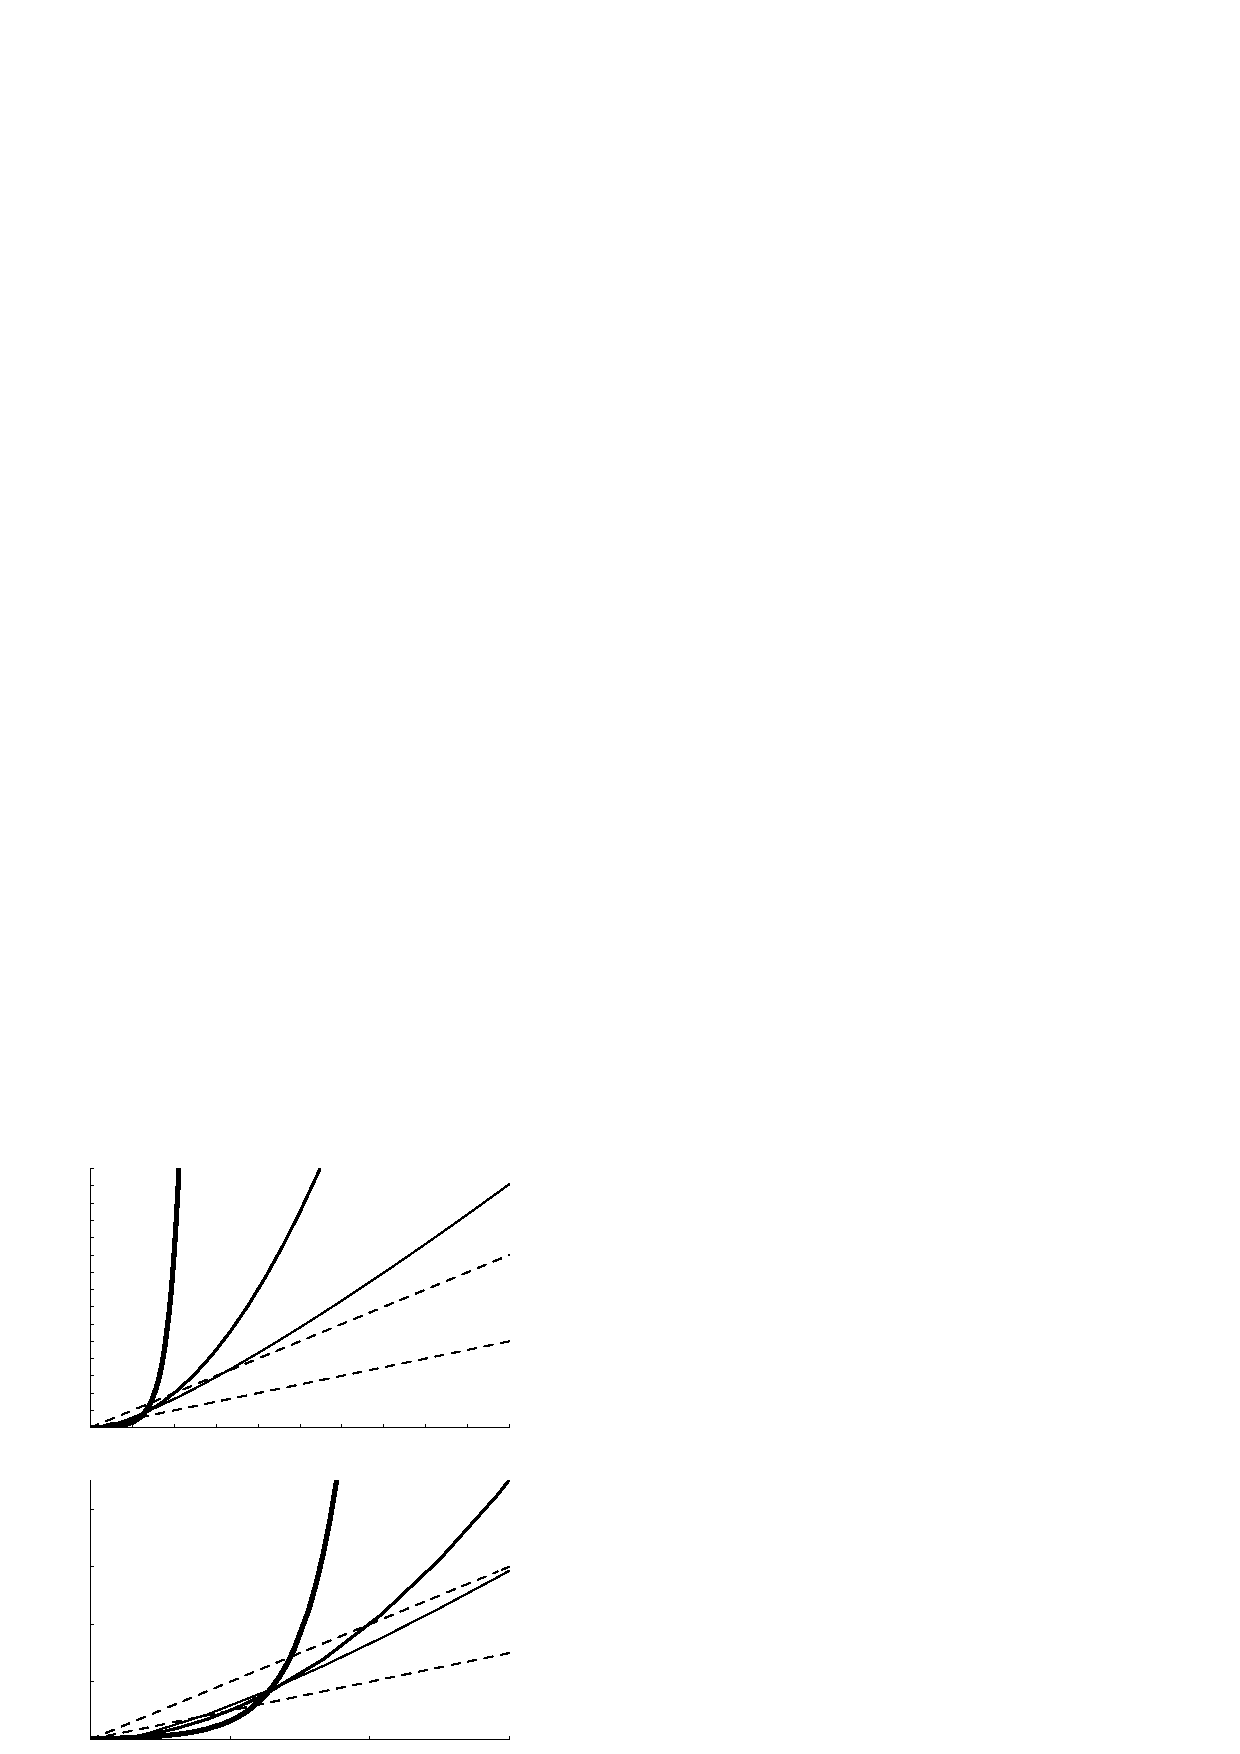
\includegraphics[viewport= 122 200 300 625]{../figs/plot.pdf}
\capt{4.5in}{The growth rates for five equations}
{Two views of a graph illustrating the growth rates for
six equations.
The bottom view shows in detail the lower-left portion
of the top view.
The horizontal axis represents input size.
The vertical axis can represent time, space, or any other measure of
cost.}
{RunTimeGraph}
\bigskip
\end{figure}

The \defit{growth rate} for an algorithm is the rate at which the cost 
of the algorithm grows as the size of its input grows.
Figure~\ref{RunTimeGraph} shows a graph for six equations, each meant
to describe the running time for a particular program or algorithm.
A variety of growth rates representative of typical
algorithms are shown.
The two equations labeled \(10n\) and \(20n\) are graphed by straight
lines.
A growth rate of \cn\ (for \(c\) any positive constant) is
often referred to as a
\defit{linear} growth rate\index{growth rate!linear} or running time. 
This means that as the value of \(n\) grows, the running time of the
algorithm grows in the same proportion.
Doubling the value of \(n\) roughly doubles the running time.
An algorithm whose running-time equation has a highest-order term
containing a factor of \(n^2\) is said to have a \defit{quadratic}
growth rate.\index{growth rate!quadratic}
In Figure~\ref{RunTimeGraph}, the line labeled \(2n^2\) represents a
quadratic growth rate.
The line labeled \(2^n\) represents an \defit{exponential}
growth rate.
\index{growth rate!exponential}
This name comes from the fact that \(n\) appears in the exponent.
The line labeled \(n!\) is also growing exponentially.

As you can see from Figure~\ref{RunTimeGraph}, the difference between
an algorithm whose running time has cost \(\Tn = 10n\) and another
with cost \(\Tn = 2n^2\) becomes tremendous as \(n\) grows.
For \(n > 5\), the algorithm with running time \(\Tn = 2n^2\) is
already much slower.
This is despite the fact that \(10n\) has a greater constant factor
than \(2n^2\).
Comparing the two curves marked \(20n\) and \(2n^2\) shows that
changing the constant factor for one of the equations only shifts the
point at which the two curves cross.
For \(n>10\), the algorithm with cost \(\Tn = 2n^2\) is slower than
the algorithm with cost \(\Tn = 20n\).
This graph also shows that the equation \(\Tn = 5 n \log n\)
grows somewhat more quickly than both \(\Tn = 10 n\) and
\(\Tn = 20 n\), but not nearly so quickly as the equation
\(\Tn = 2n^2\). 
For constants \(a, b > 1\), \(n^a\)~grows faster than either
\(\log^b n\) or \(\log n^b\).
Finally, algorithms with cost \(\Tn = 2^n\) or \(\Tn = n!\) are
prohibitively expensive for even modest values of \(n\).
Note that for constants \(a, b \geq 1\), \(a^n\)~grows faster than
\(n^b\).

We can get some further insight into relative growth rates for various
algorithms from Figure~\ref{GrowthTable}.
Most of the growth rates that appear in typical algorithms are shown,
along with some representative input sizes.
Once again, we see that the growth rate has a tremendous effect on the
resources consumed by an algorithm.

\begin{mytable}
{\sffamily
\[
\begin{array}
{c|c|c|c|c|c|c|c}
\mathsf{n} & \mathsf{\log \log n} & \mathsf{\log n} & \mathsf{n} &
\mathsf{n \log n} & \mathsf{n^2} & \mathsf{n^3} & \mathsf{2^n}\\
\hline
\mathsf{16} & \mathsf{2} & \mathsf{4} & \mathsf{2^{4}} &
\mathsf{4 \cdot 2^{4} = 2^{6}}\rule{0pt}{12pt} &
\mathsf{2^{8}} & \mathsf{2^{12}} & \mathsf{2^{16}}\\
\mathsf{256} & \mathsf{3} & \mathsf{8} & \mathsf{2^{8}} &
\mathsf{8 \cdot 2^{8} = 2^{11}} &
\mathsf{2^{16}} & \mathsf{2^{24}} & \mathsf{2^{256}}\\
\mathsf{1024} & \mathsf{\approx 3.3} & \mathsf{10} & \mathsf{2^{10}} &
\mathsf{10 \cdot 2^{10} \approx 2^{13}} &
\mathsf{2^{20}} & \mathsf{2^{30}} & \mathsf{2^{1024}}\\
\mathsf{64 {\rm K}} & \mathsf{4} & \mathsf{16} & \mathsf{2^{16}} &
\mathsf{16 \cdot 2^{16} = 2^{20}} &
\mathsf{2^{32}} & \mathsf{2^{48}} & \mathsf{2^{64 {\rm K}}}\\
\mathsf{1 {\rm M}} & \mathsf{\approx 4.3} & \mathsf{20} & \mathsf{2^{20}} &
\mathsf{20 \cdot 2^{20} \approx 2^{24}} &
\mathsf{2^{40}} & \mathsf{2^{60}} & \mathsf{2^{1 {\rm M}}}\\
\mathsf{1 {\rm G}} & \mathsf{\approx 4.9} & \mathsf{30} & \mathsf{2^{30}} &
\mathsf{30 \cdot 2^{30} \approx 2^{35}} &
\mathsf{2^{60}} & \mathsf{2^{90}} & \mathsf{2^{1 {\rm G}}}\\
\end{array}
\]
}
\vspace{-\bigskipamount}
\vspace{-\bigskipamount}
\capt{4.5in}{Costs for representative growth rates}
{Costs for growth rates representative of most computer
algorithms.}{GrowthTable}
\end{mytable}

\index{growth rate|)}

\newpage

\section{Best, Worst, and Average Cases}

\index{best-case analysis|(}
\index{worst-case analysis|(}
\index{average-case analysis|(}

Consider the problem of finding the factorial of \(n\).
For this problem, there is only one input of a given ``size'' (that
is, there is only a single instance for each size of \(n\)).
Now consider our largest-value sequential search
algorithm of Example~\ref{SeqMax}, which always examines every array
value.\index{search!sequential}
This algorithm works on many inputs of a given size \(n\).
That is, there are many possible arrays of any given size.
However, no matter what array of size \(n\) that the algorithm looks
at, its cost will always be the same in that it always looks at every
element in the array one time.

For some algorithms, different inputs of a given size require
different amounts of time.\index{input size}
For example, consider the problem of searching an array containing
\(n\) integers to find the one with a particular value \(K\)
(assume that \(K\) appears exactly once in the array).
\index{search!sequential|(}
The \defit{sequential search} algorithm begins
at the first position in the array and looks at each value in turn
until \(K\) is found.
Once \(K\) is found, the algorithm stops.
This is different from the largest-value sequential search
algorithm of Example~\ref{SeqMax}, which always examines every array
value.\index{search!sequential}

There is a wide range of possible running
times for the sequential search algorithm.
The first integer in the array could have value \(K\), and so only one
integer is examined.
In this case the running time is short.
This is the \defit{best case} for this algorithm, because it is not
possible for sequential search to look at less than one value.
Alternatively, if the last position in the array contains \(K\),
then the running time is relatively long, because the algorithm
must examine \(n\) values.
This is the \defit{worst case} for
this algorithm, because sequential search never looks at more than
\(n\) values.
If we implement sequential search as a program and run it many times
on many different arrays of size \(n\),
or search for many different values of \(K\) within the same array,
we expect the algorithm on average to go halfway through the array
before finding the value we seek.
On average, the algorithm examines about \(n/2\) values.
We call this the \defit{average case} for this algorithm.

When analyzing an algorithm, should we study the best, worst, or
average case?
Normally we are not interested in the best case, because this might
happen only rarely and generally is too optimistic for a fair
characterization of the algorithm's running time.
In other words, analysis based on the best case is not likely to be
representative of the behavior of the algorithm.
However, there are rare instances where a best-case analysis is
useful --- in particular, when the best case has high probability of
occurring.
In Chapter~\ref{InSort}\index{sorting} you will see some examples
where taking advantage of the best-case running time for one sorting
algorithm makes a second more efficient.

How about the worst case?
The advantage to analyzing the worst case is that you know for
certain that the algorithm must perform at least that well.
This is especially important for real-time applications,
\index{real-time applications}
such as for the computers that monitor an air traffic control system.
Here, it would not be acceptable to use an algorithm that can handle
\(n\) airplanes quickly enough \emph{most of the time}, but which
fails to perform quickly enough when all \(n\)~airplanes are coming
from the same direction.

For other applications --- particularly when we wish to aggregate the
cost of running the program many times on many different inputs ---
worst-case analysis might not be a representative measure of the
algorithm's performance.
Often we prefer to know the average-case running time.
This means that we would like to know the \emph{typical} behavior of
the algorithm on inputs of size \(n\).
Unfortunately, average-case analysis is not always possible.
Average-case analysis first requires that we understand how the actual
inputs to the program (and their costs) are distributed with respect
to the set of all possible inputs to the program.
For example, it was stated previously that the sequential search
algorithm on average examines half of the array values.
This is only true if the element with value \(K\) is
equally likely to appear in any position in the array.
If this assumption is not correct, then the algorithm does \emph{not}
necessarily examine half of the array values in the average case.
See Section~\ref{SelfOrg} for further discussion regarding the effects
of data distribution on the sequential search algorithm.
\index{search!sequential|)}

The characteristics of a data distribution have a significant effect
on many search algorithms, such as those based on
hashing\index{hashing} (Section~\ref{Hash}) and search
trees\index{search trees} (e.g., see Section~\ref{BST}).
Incorrect assumptions about data distribution can have disastrous
consequences on a program's space or time performance.
Unusual data distributions can also be used to advantage, as shown in
Section~\ref{SelfOrg}.\index{list!self-organizing}

In summary, for real-time applications\index{real-time applications}
we are likely to prefer a worst-case analysis of an algorithm.
Otherwise, we often desire an average-case analysis if we know enough
about the distribution of our input to compute the average case.
If not, then we must resort to worst-case analysis.
\index{average-case analysis|)}
\index{worst-case analysis|)}
\index{best-case analysis|)}

\section{A Faster Computer, or a Faster Algorithm?}

Imagine that you have a problem to solve, and you know of an algorithm
whose running time is proportional to \(n^2\).
Unfortunately, the resulting program takes ten times too long to run.
If you replace your current computer with a new one that is ten times
faster, will the \(n^2\) algorithm become acceptable?
If the problem size remains the same, then perhaps
the faster computer will allow you to get your work done quickly
enough even with an algorithm having a high growth rate.
But a funny thing happens to most people who get a faster computer.
They don't run the same problem faster.
They run a bigger problem!
Say that on your old computer you were content to sort\index{sorting}
10,000 records because that could be done by the computer during your
lunch break.
On your new computer you might hope to sort 100,000
records in the same time.
You won't be back from lunch any sooner, so you are better off solving a
larger problem.
And because the new machine is ten times faster, you would like to
sort ten times as many records.
\index{sorting}

If your algorithm's growth rate is linear (i.e., if the equation that
describes the running time on input size \(n\) is \(\Tn = \cn\) for some
constant \(c\)),\index{growth rate!linear}
then 100,000 records on the new machine will be sorted in the same time
as 10,000 records on the old machine.
If the algorithm's growth rate is greater than \cn,
such as \(c_1n^2\), then you will \emph{not} be able to do a
problem ten times the size in the same amount of time on a machine
that is ten times faster.\index{growth rate!quadratic}

How much larger a problem can be solved
in a given amount of time by a faster computer?
Assume that the new machine is ten times faster than the old.
Say that the old machine could solve a problem of size \(n\) in an hour.
What is the largest problem that the new machine can solve in one hour?
Figure~\ref{Speedups} shows how large a problem can be solved on
the two machines for five of the running-time functions from
Figure~\ref{RunTimeGraph}.

\begin{mytable}
{\sffamily
\[
\begin{array}
{l|r|r|l|r}
\multicolumn{1}{c}{\mbox{\sffamily\textbf{f(n)}}} &
\multicolumn{1}{|c}{\mbox{\sffamily\textbf{n}}} & 
\multicolumn{1}{|c}{\mbox{\sffamily\textbf{n\boldmath$'$}}} &
\multicolumn{1}{|c}{\mbox{\sffamily\textbf{Change}}} &
\multicolumn{1}{|c}{\mbox{\sffamily\textbf{n\boldmath$'$/n}}}\\
\hline
\mathsf{10n}     & \mathsf{1000} & \mathsf{10,000} & \mathsf{n' = 10n} & \mathsf{10}\\
\mathsf{20n}     & \mathsf{500}   & \mathsf{5000}  & \mathsf{n' = 10n} & \mathsf{10}\\
\mathsf{5 n\:log\:n} & \mathsf{250} & \mathsf{1842} & \mathsf{\sqrt{10} n < n' < 10n} & \mathsf{7.37}\\
\mathsf{2 n^2}   & \mathsf{70}    & \mathsf{223}    & \mathsf{n' = \sqrt{10} n} & \mathsf{3.16}\\
\mathsf{2^n}     & \mathsf{13}    & \mathsf{16}     & \mathsf{n' = n + 3} & \mathsf{--}\\
\end{array}
\]
}
\capt{4.5in}{The increase in problem size for a computer ten times faster}
{The increase in problem size that can be run
in a fixed period of time on a computer that is ten times faster.
The first column lists the right-hand sides for each of five
growth rate equations from Figure~\ref{RunTimeGraph}.
For the purpose of this example, arbitrarily assume that the old
machine can run 10,000 basic operations\index{basic operation}
in one hour.
The second column shows the maximum value for \(n\) that can be run
in 10,000 basic operations on the old machine.
The third column shows the value for \(n'\), the new maximum
size for the problem that can be run in the same time on the new
machine that is ten times faster.
Variable \(n'\) is the greatest size for the problem that can run in
100,000 basic operations.
The fourth column shows how the size of \(n\) changed to become \(n'\) on
the new machine.
The fifth column shows the increase in the problem size as the ratio of
\(n'\) to \(n\).}
{Speedups}
\bigskip\smallskip
\end{mytable}

This table illustrates many important points.
\index{growth rate!linear}
The first two equations are both linear; only the value of the
constant factor has changed.
In both cases, the machine that is ten times faster gives an increase
in problem size by a factor of ten.
In other words, while the value of the constant
does affect the absolute size of the problem that can be solved in a
fixed amount of time, it does not affect the \emph{improvement} in
problem size (as a proportion to the original size) gained by a faster
computer.
This relationship holds true regardless of the algorithm's growth
rate:
Constant factors never affect the relative improvement gained
by a faster computer.
\index{growth rate!linear}

\index{growth rate!quadratic}
An algorithm with time equation \(\Tn = 2n^2\) does not receive nearly
as great an improvement from the faster machine as an algorithm with
linear growth rate.
Instead of an improvement by a factor of ten, the improvement
is only the square root of that: \(\sqrt{10} \approx 3.16\).
Thus, the algorithm with higher growth rate not only solves a smaller
problem in a given time in the first place, it \emph{also}
receives less of a speedup from a faster computer.
As computers get ever faster, the disparity in problem sizes becomes
ever greater.

The algorithm with growth rate \(\Tn = 5 n \log n\) improves by a
greater amount than the one with quadratic growth rate, but not
by as great an amount as the algorithms with linear growth rates.

\index{growth rate!exponential}
Note that something special happens in the case of the
algorithm whose running time grows exponentially.
In Figure~\ref{RunTimeGraph}, the curve for the algorithm whose time
is proportional to \(2^n\) goes up very quickly.
In Figure~\ref{Speedups}, the increase in problem size on the machine
ten times as fast is shown to be about \(n + 3\)
(to be precise, it is \(n + \log_2 10\)).
The increase in problem size for an algorithm with exponential growth
rate is by a constant addition, not by a multiplicative factor.
Because the old value of \(n\) was~13, the new problem size is~16.
If next year you buy another computer ten times faster yet, then the
new computer (100 times faster than the original computer) will only
run a problem of size~19.
If you had a second program whose growth rate is \(2^n\) and for which
the original computer could run a problem of size~1000 in an hour,
than a machine ten times faster can run a problem only of size~1003 in
an hour!
Thus, an exponential growth rate is radically different than the
other growth rates shown in Figure~\ref{Speedups}.
The significance of this difference is explored in
Chapter~\ref{LimComp}.
\index{growth rate!exponential}

\index{growth rate!quadratic}
Instead of buying a faster computer,
consider what happens if you replace an algorithm whose
running time is proportional to \(n^2\) with a new
algorithm whose running time is proportional to \(n \log n\).
In the graph of Figure~\ref{RunTimeGraph}, a fixed amount of time would
appear as a horizontal line.
If the line for the amount of time available to solve your problem
is above the point at which the curves for the two growth rates in
question meet, then the algorithm whose running time grows less
quickly is faster.
An algorithm with running time \(\Tn=n^2\) requires
\(1024 \times 1024 = 1,048,576\) time steps for an input of size
\(n=1024\).
An~algorithm with running time \(\Tn=n\log n\) requires
\(1024\times 10=10,240\) time steps for an input of size
\(n = 1024\), which is an improvement of much more than a factor of ten
when compared to the algorithm with running time \(\Tn = n^2\).
Because \(n^2 > 10 n \log n\) whenever \(n > 58\), if the typical
problem size is larger than 58 for this example, then you would be
much better off changing algorithms instead of buying a computer ten
times faster.
Furthermore, when you do buy a faster computer, an algorithm with a
slower growth rate provides a greater benefit in terms of larger
problem size that can run in a certain time on the new computer.
\index{growth rate!quadratic}

\newpage

\section{Asymptotic Analysis}

\index{algorithm analysis!asymptotic|(}
Despite the larger constant for the curve labeled
\(10 n\) in Figure~\ref{RunTimeGraph}, \(2 n^2\)
crosses it at the relatively small value of \(n = 5\).
What if we double the value of the constant in front of the linear
equation?\index{growth rate!linear}
As shown in the graph, \(20 n\) is surpassed by \(2 n^2\)
once \(n = 10\).
The additional factor of two for the linear growth rate does not much
matter.
It only doubles the \(x\)-coordinate for the intersection point.
In general, changes to a constant factor in either equation only
shift \emph{where} the two curves cross, not \emph{whether}
the two curves cross.

\index{growth rate!asymptotic|(}
When you buy a faster computer or a faster compiler,
the new problem size that can be run in a given amount of time for a
given growth rate is
larger by the same factor, regardless of the constant on the
running-time equation.
The time curves for two algorithms with different growth rates
still cross, regardless of their running-time equation constants.
For these reasons, we usually ignore the constants when we want an
estimate of the growth rate for the running time or other resource
requirements of an algorithm.
This simplifies the analysis and keeps us thinking about the most
important aspect: the growth rate.
This is called \defit{asymptotic algorithm analysis}.
To be precise, asymptotic analysis refers to the study of an
algorithm as the input size ``gets big'' or reaches
a limit (in the calculus sense).
However, it has proved to be so useful to ignore all constant factors
that asymptotic analysis is used for most algorithm comparisons.

It is not always reasonable to ignore the constants.
When comparing algorithms meant to run on small values of \(n\),
the constant can have a large effect.
For example, if the problem is to sort a collection of exactly
five records, then an algorithm designed for sorting thousands of
records is probably not appropriate, even if its asymptotic analysis
indicates good performance.
There are rare cases where the constants for two algorithms under
comparison can differ by a factor of 1000 or more, making the one
with lower growth rate impractical for most purposes due to its large
constant.
Asymptotic analysis is a form of ``back of the envelope''
estimation\index{estimation} for algorithm resource consumption.
It provides a simplified model of the running time or
other resource needs of an algorithm.
This simplification usually helps you understand the behavior of your
algorithms.
Just be aware of the limitations to asymptotic analysis in the
rare situation where the constant is important.
\index{growth rate!asymptotic|)}

\subsection{Upper Bounds}

\index{upper bound|(}
Several terms are used to describe the running-time equation for an
algorithm.
These terms --- and their associated symbols --- indicate precisely what
aspect of the algorithm's behavior is being described.
One is the \defit{upper bound} for the growth of the algorithm's
running time.
It indicates the upper or highest growth rate that
the algorithm can have.

\index{o notation@O notation|(}
Because the phrase
``has an upper bound to its growth rate of \(f(n)\)''
is long and often used when discussing algorithms, we adopt a
special notation, called \defit{big-Oh notation}.
If the upper bound for an algorithm's growth rate (for, say, the
worst case) is \(f(n)\), then we would write that this algorithm is
``in the set \Ofn in the worst case''
(or just ``in \Ofn in the worst case'').
For example, if \(n^2\) grows as fast as \Tn\ (the running
time of our algorithm) for the worst-case input,
we would say the algorithm is ``in \Ontwo\ in the worst case.''

The following is a precise definition for an upper bound.
\Tn\ represents the true running time of the algorithm.
\(f(n)\) is some expression for the upper bound.

\begin{quotation}
For \Tn\ a non-negatively valued function,
\Tn\ is in set \Ofn\ if there exist two positive
constants \(c\) and \(n_0\) such that \(\Tn \leq cf(n)\) for all
\(n > n_0\).
\end{quotation}

\noindent Constant \(n_0\) is the smallest value of \(n\) for which the
claim of an upper bound holds true.
Usually \(n_0\) is small, such as 1, but does not need to be.
You must also be able to pick some constant \(c\), but it is irrelevant
what the value for \(c\) actually is.
In other words, the definition says that for \emph{all} inputs of the
type in question (such as the worst case for all inputs of size~\(n\))
that are large enough (i.e., \(n > n_0\)), the algorithm \emph{always}
executes in less than \(cf(n)\) steps for some constant \(c\).

\begin{example}
Consider the sequential search algorithm for finding a specified value
in an array of integers.\index{search!sequential}
If visiting and examining one value in the array requires \(c_s\)
steps where \(c_s\) is a positive number,
and if the value we search for has equal probability of appearing in
any position in the array,
then in the average case \(\Tn = c_s n/2\).
For all values of \(n > 1\), \( c_s n/2 \leq c_s n\).
Therefore, by the definition, \Tn\ is in \On\ for \(n_0 = 1\) and
\(c = c_s\).
\end{example}

\begin{example}
For a particular algorithm, \(\Tn = c_1 n^2 + c_2 n\) in the
average case where \(c_1\) and \(c_2\) are positive numbers.
Then,
\(c_1 n^2 + c_2 n \leq c_1 n^2 + c_2 n^2 \leq (c_1 + c_2)n^2\)
for all \(n > 1\).
So, \(\Tn \leq c n^2\) for \(c = c_1 + c_2\), and \(n_0 = 1\).
Therefore, \Tn\ is in \Ontwo\ by the second definition.
\end{example}

\begin{example}
Assigning the value from the first position of an array to a variable
takes constant time regardless of the size of the
array.\index{growth rate!constant}
Thus, \(\Tn = c\) (for the best, worst, and average cases).
We could say in this case that \Tn\ is in \Oc.
However, it is traditional to say that an algorithm whose running time
has a constant upper bound is in \Oone.
\end{example}

\index{worst-case analysis}
If someone asked you out of the blue ``Who is the best?'' your natural
reaction should be to reply ``Best at what?''
In the same way, if you are asked ``What is the growth rate of this
algorithm,'' you would need to ask ``When? Best case? Average case? Or
worst case?''
Some algorithms have the same behavior no matter which input instance
they receive.
An example is finding the maximum in an array of integers.
But for many algorithms, it makes a big difference, such as when
searching an unsorted array for a particular value.
So any statement about the upper bound of an algorithm
must be in the context of some class of inputs of size \(n\).
We~measure this upper bound nearly always on the best-case,
average-case, or worst-case inputs.
Thus, we cannot say, ``this algorithm has an upper bound to its growth
rate of \(n^2\).''
We must say something like, ``this algorithm has an upper bound to its
growth rate of \(n^2\) \emph{in the average case}.''
\index{worst-case analysis}

Knowing that something is in \Ofn\ says only how bad things can be.
Perhaps things are not nearly so bad.
Because sequential search\index{search!sequential} is in \On\
in the worst case,
it is also true to say that sequential search is in \Ontwo.
But sequential search is practical for large \(n\), in a way that is
not true for some other algorithms in \Ontwo.
We always seek to define the running time of an algorithm
with the tightest (lowest) possible upper bound.
Thus, we prefer to say that sequential search is in \On.
This also explains why the phrase ``is in \Ofn'' or the notation
``\(\in \Ofn\)'' is used instead of ``is~\Ofn'' or ``\(= \Ofn\).''
There is no strict equality to the use of big-Oh notation.
\On\ is in \Ontwo, but \Ontwo\ is not in \On.
\index{upper bound|)}

\subsection{Lower Bounds}

\index{lower bound|(}
Big-Oh notation describes an upper bound.
In other words, big-Oh notation states a claim about the greatest
amount of some resource (usually time) that is required by an
algorithm for some class of inputs of size \(n\) (typically
the worst such input, the average of all possible inputs, or the best
such input).

Similar notation is used to describe the least amount of a resource
that an algorithm needs for some class of input.
Like big-Oh notation, this is a measure of the algorithm's
growth rate.
Like big-Oh notation, it works for any resource, but
we most often measure the least amount of time required.
And again, like big-Oh notation, we are measuring the resource
required for some particular class of inputs: the worst-, average-,
or best-case input of size~\(n\).

\index{omega notation@\(\Omega\) notation|(}
The lower bound for an algorithm (or a problem, as explained later)
is denoted by the symbol \(\Omega\), pronounced ``big-Omega'' or just
``Omega.''
The following definition for \(\Omega\) is symmetric with the
definition of big-Oh.

\begin{quotation}
For \Tn\ a non-negatively valued function,
\Tn\ is in set \Omegagn\ if there exist two positive
constants \(c\) and \(n_0\) such that \(\Tn \geq c g(n)\) for all
\(n > n_0\).\footnote{
An alternate (non-equivalent) definition for \(\Omega\) is

\begin{quotation}
\Tn\ is in the set \Omegagn\ if there exists a positive constant
\(c\) such that \(\Tn \geq c g(n)\) for an infinite number of
values for \(n\).
\end{quotation}

This definition says that for an ``interesting'' number of
cases, the algorithm takes at least \(c g(n)\) time.
Note that this definition is \emph{not} symmetric with the definition
of big-Oh.
For \(g(n)\) to be a lower bound,
this definition \emph{does not} require that \(\Tn \geq c g(n)\) for
all values of \(n\) greater than some constant.
It only requires that this happen often enough, in particular that it
happen for an infinite number of values for \(n\).
Motivation for this alternate definition can be found in the
following example.

Assume a particular algorithm has the following behavior:

\vspace{-\smallskipamount}
\[\Tn = \left\{ \begin{array}{ll}
		n       & \mbox{for all odd}\ n \geq 1\\
		n^2/100 & \mbox{for all even}\ n \geq 0
               \end{array}
        \right. \]

\vspace{-\smallskipamount}
From this definition, \(n^2/100 \geq \frac{1}{100} n^2\) for all even
\(n \geq 0\).
So, \(\Tn \geq c n^2\) for an infinite number of values of \(n\)
(i.e., for all even \(n\)) for \(c = 1/100\).
Therefore, \Tn\ is in \Omegantwo\ by the definition.

For this equation for \Tn, it is true that all inputs
of size \(n\) take at least \cn\ time.
But an infinite number of inputs of size \(n\) take \cntwo\ time,
so we would like to say that the algorithm is in \Omegantwo.
Unfortunately, using our first definition will
yield a lower bound of \Omegan\ because it is not possible to pick
constants \(c\) and \(n_0\) such that \(\Tn \geq c n^2\) for all
\(n>n_0\).
The alternative definition does result in a lower
bound of \Omegantwo\ for this algorithm, which seems to fit common
sense more closely.
Fortunately, few real algorithms or computer programs display the
pathological behavior of this example.
Our first definition for \(\Omega\) generally yields the expected
result.

As you can see from this discussion, asymptotic bounds notation is
not a law of nature.
It is merely a powerful modeling tool used to describe the behavior
of algorithms.} % end of footnote
\end{quotation}

\begin{example}
\label{AAnalEx}
Assume \(\Tn = c_1 n^2 + c_2 n\) for \(c_1\) and \(c_2 > 0\).
Then,
\[c_1 n^2 + c_2 n \geq c_1 n^2\]
for all \(n > 1\).
So, \(\Tn \geq c n^2\) for \(c = c_1\) and \(n_0 = 1\).
Therefore, \Tn\ is in \Omegantwo\ by the definition.
\end{example}

It is also true that the equation of Example~\ref{AAnalEx} is in
\Omegan.
However, as with big-Oh notation, we wish to get the ``tightest''
(for \(\Omega\)~notation, the largest) bound possible.
Thus, we prefer to say that this running time is in \Omegantwo.

Recall the sequential search algorithm to find a value~\(K\)
within an array of integers.
In the average and worst cases this algorithm is in \Omegan,
because in both the average and worst cases we must examine
\emph{at least} \(cn\) values (where~\(c\) is~\(1/2\) in the average
case and~1 in the worst case).
\index{omega notation@\(\Omega\) notation|)}
\index{lower bound|)}

\subsection{$\Theta$ Notation}

\index{upper bound|(}\index{lower bound|(}
\index{theta notation@\(\Theta\) notation}
The definitions for big-Oh and
\(\Omega\)\index{omega notation@\(\Omega\) notation} give us ways to
describe the upper bound for an algorithm (if we can find an equation
for the maximum cost of a particular class of inputs of size \(n\))
and the lower bound for an algorithm
(if we can find an equation for the minimum cost for
a particular class of inputs of size \(n\)).
When the upper and lower bounds are the same within a constant factor,
we indicate this by using \(\Theta\) (big-Theta) notation.
An algorithm is said to be \Thetahn\ if it is in \Ohn\ \emph{and} it
is in \Omegahn.
Note that we drop the word ``in'' for \(\Theta\)~notation,
because there is a strict equality for two equations with the
same~\(\Theta\).
In other words, if \(f(n)\) is \Thetagn, then \(g(n)\) is~\Thetafn.

Because the sequential search algorithm is both in \On\ and in
\Omegan\ in the average case, we say it is \Thetan\ in the average
case.

Given an algebraic equation describing the time requirement for
an algorithm, the upper and lower bounds always meet.
That is because in some sense we have a perfect analysis for the
algorithm, embodied by the running-time equation.
For many algorithms (or their instantiations as programs), it is easy
to come up with the equation that defines their runtime behavior.
Most algorithms presented in this book are well understood and we can
almost always give a \(\Theta\) analysis for them.
However, Chapter~\ref{LimComp} discusses a whole class of
algorithms for which we have no \(\Theta\) analysis, just some
unsatisfying big-Oh and \(\Omega\) analyses.
Exercise~\ref{AlgAnal}.\ref{Collatz}
presents a short,
simple program fragment\index{collatz sequence@Collatz sequence}
for which nobody currently knows the true upper or lower bounds.

While some textbooks and programmers will casually say that an
algorithm is ``order of'' or ``big-Oh'' of some cost function,
it is generally better to use \(\Theta\) notation rather than big-Oh
notation whenever we have sufficient knowledge about an algorithm to
be sure that the upper and lower bounds indeed match.
Throughout this book, \(\Theta\) notation will be used in preference to
big-Oh notation whenever our state of knowledge makes that possible.
Limitations on our ability to analyze certain algorithms may require
use of big-Oh or \(\Omega\) notations.
In rare occasions when the discussion is explicitly about the upper or 
lower bound of a problem or algorithm, the corresponding notation will
be used in preference to \(\Theta\) notation.
\index{theta notation@\(\Theta\) notation}
\index{lower bound|)}\index{upper bound|)}

\subsection{Simplifying Rules}
\label{SimpRule}

\index{omega notation@\(\Omega\) notation|(}
\index{theta notation@\(\Theta\) notation|(}
Once you determine the running-time equation for an algorithm,
it really is a simple matter to derive the big-Oh, \(\Omega\), and
\(\Theta\) expressions from the equation.
You do not need to resort to the formal definitions of asymptotic
analysis.
Instead, you can use the following rules to
determine the simplest form.

\begin{enumerate}

\item
If \(f(n)\) is in \Ogn\ and \(g(n)\) is in \Ohn, then \(f(n)\) is in
\Ohn.

\item
If \(f(n)\) is in \({\rm O}(k g(n))\) for any constant \(k > 0\),
then \(f(n)\) is in \Ogn.

\item
If \(f_1(n)\) is in \({\rm O}(g_1(n))\) and \(f_2(n)\) is in
\({\rm O}(g_2(n))\),
then \(f_1(n) + f_2(n)\) is in \({\rm O}(\max(g_1(n), g_2(n)))\).

\item
If \(f_1(n)\) is in \({\rm O}(g_1(n))\) and \(f_2(n)\) is in
\({\rm O}(g_2(n))\), then \(f_1(n) f_2(n)\) is in
\({\rm O}(g_1(n) g_2(n))\).

\end{enumerate}

The first rule says that if some function \(g(n)\) is an upper bound
for your cost function, then any upper bound for \(g(n)\) is also an
upper bound for your cost function.\index{upper bound}
A similar property holds true for \(\Omega\) notation:
If \(g(n)\) is a lower bound for your cost function, then any lower
bound for \(g(n)\) is also a lower bound for your cost function.
Likewise for \(\Theta\) notation.\index{lower bound}

The significance of rule (2) is that you can ignore any multiplicative
constants in your equations when using big-Oh notation.
This rule also holds true for \(\Omega\) and \(\Theta\) notations.

Rule (3) says that given two parts of a program run in sequence
(whether two statements or two sections of code),
you need consider only the more expensive part.
This rule applies to \(\Omega\) and \(\Theta\) notations as well:
For both, you need consider only the more expensive part.

Rule (4) is used to analyze simple loops in programs.
If some action is repeated some number of times,
and each repetition has the same cost, then the total cost
is the cost of the action multiplied by the number of times that the
action takes place.
This rule applies to \(\Omega\) and \(\Theta\) notations as well.

Taking the first three rules collectively, you can ignore all
constants and all lower-order terms to determine the asymptotic growth
rate for any cost function.
The advantages and dangers of ignoring constants were discussed near
the beginning of this section.
Ignoring lower-order terms is reasonable when performing an
asymptotic analysis.
The higher-order terms soon swamp the lower-order terms in their
contribution to the total cost as \(n\) becomes larger.
Thus, if \(\Tn = 3 n^4 + 5 n^2\), then \Tn\ is in \Onfour.
The \(n^2\) term contributes relatively little to the total cost for
large \(n\).

Throughout the rest of this book, these simplifying
rules are used when discussing the cost for a program or algorithm.
\index{theta notation@\(\Theta\) notation|)}
\index{omega notation@\(\Omega\) notation|)}
\index{o notation@O notation|)}
\index{algorithm analysis!asymptotic|)}

\subsection{Classifying Functions}
\label{ClassifyFuncs}

Given functions \fn\ and \gn\ whose growth rates are expressed as
algebraic equations, we might like to determine if one grows faster
than the other.
The best way to do this is to take the limit of the two
functions as \(n\) grows towards infinity,
\[\lim_{n \rightarrow \infty} \frac{f(n)}{g(n)}.\]
If the limit goes to \(\infty\), then \fn\ is in \Omegagn\ because
\fn\ grows faster.
If the limit goes to zero, then \fn\ is in \Ogn\ because \gn\ grows
faster.
If the limit goes to some constant other than zero, then
\(f(n) = \Theta(g(n))\) because both grow at the same rate.

\begin{example}
If \(f(n) = 2n\log n\) and \(g(n)=n^2\), is \fn\ in \Ogn, \Omegagn, or
\Thetagn?
Because
\[\frac{n^2}{2n\log n} = \frac{n}{2\log n},\]
we easily see that
\[\lim_{n \rightarrow \infty} \frac{n^2}{2n\log n} = \infty\]
because \(n\) grows faster than \(2\log n\).
Thus, \(n^2\) is in \(\Omega(2n\log n)\).
\end{example}

\section{Calculating the Running Time for a Program}
\label{ProgTimeSec}

\index{algorithm analysis!for program statements|(}
This section presents the analysis for several simple code
fragments.

\begin{example}
We begin with an analysis of a simple assignment to an integer
variable.

\vspace{-\medskipamount}
\xprogexamp{c3p2.book}

\vspace{-\medskipamount}
\noindent Because the assignment statement takes constant time, it is
\Thetaone.
\end{example}

\begin{example}
\label{FLAnal}
Consider a simple \Cref{for} loop.

\vspace{-\medskipamount}
\xprogexamp{c3p3.book}

\vspace{-\medskipamount}
The first line is~\Thetaone.
The \Cref{for} loop is repeated \(n\) times.
The third line takes constant time so, by simplifying rule~(4)
of Section~\ref{SimpRule}, the total cost for executing the two lines
making up the \Cref{for} loop is \Thetan.
By rule~(3), the cost of the entire code fragment is also
\Thetan.
\end{example}

\begin{example}
We now analyze a code fragment with several \Cref{for}
loops, some of which are nested.

\vspace{-\medskipamount}
\xprogexamp{c3p4.book}

\vspace{-\medskipamount}
This code fragment has three separate statements: the
first assignment statement and the two \Cref{for} loops.
Again the assignment statement takes constant time;
call it \(c_1\).
The second \Cref{for} loop is just like the one in
Example~\ref{FLAnal} and takes \(c_2 n\) = \Thetan\ time.

The first \Cref{for} loop is a double loop and requires a special
technique.
We work from the inside of the loop outward.
The expression \Cref{sum++} requires constant time; call it \(c_3\).
Because the inner \Cref{for} loop is executed \(i\)~times,
by simplifying rule (4) it has cost \(c_3i\).
The outer \Cref{for} loop is executed \(n\)~times, but each time
the cost of the inner loop is different because it costs \(c_3i\) with
\(i\) changing each time.
You should see that for the first execution of the outer loop,
\(i\)~is~1.
For the second execution of the outer loop, \(i\)~is~2.
Each time through the outer loop, \(i\)~becomes one greater, until
the last time through the loop when \(i = n\).
Thus, the total cost of the loop is \(c_3\) times the sum of the
integers~1 through~\(n\).\index{summation}
From Equation~\ref{Sumi}, we know that
\[\sum_{i = 1}^{n} i = \frac{n (n+1)}{2},\]
which is \Thetantwo.
By simplifying rule (3), \(\Theta(c_1 + c_2 n + c_3 n^2)\) is
simply \Thetantwo.
\end{example}

\begin{example}
Compare the asymptotic analysis for the following two code
fragments:

\xprogexamp{c3p5.book}

In the first double loop, the inner \Cref{for} loop always executes
\(n\) times.
Because the outer loop executes \(n\) times, it should be obvious
that the statement \Cref{sum1++} is executed precisely \(n^2\) times.
The second loop is similar to the one analyzed in the previous
example, with cost \(\sum_{j = 1}^{n} j\).\index{summation}
This is approximately \({1 \over 2} n^2\).
Thus, both double loops cost \Thetantwo, though the second requires
about half the time of the first.
\end{example}

\begin{example}
Not all doubly nested \Cref{for} loops are \Thetantwo.
The following pair of nested loops illustrates this fact.

\xprogexamp{c3p6.book}

When analyzing these two code fragments, we will assume that \(n\) is
a power of two.
The first code fragment has its outer \Cref{for} loop executed
\(\log n+1\) times because on each iteration~\(k\) is multiplied by
two until it reaches~\(n\).
Because the inner loop always executes \(n\) times, the total cost for
the first code fragment can be expressed as
\(\sum_{i=0}^{\log n} n\).\index{summation}
Note that a variable substitution takes place here to create the
summation, with \(k = 2^i\).
From Equation~\ref{SumLog}, the solution for this summation is
\Thetanlogn.
In the second code fragment, the outer loop is also executed
\(\log n+1\) times.
The inner loop has cost \(k\), which doubles each time.
The summation can be expressed as \(\sum_{i=0}^{\log n} 2^i\)
where~\(n\) is assumed to be a power of two and again
\(k = 2^i\).\index{summation}
From Equation~\ref{SumExLog}, we know that this summation is
simply~\Thetan.
\end{example}

What about other control statements?
\Cref{While} loops are analyzed in a manner similar to \Cref{for}
loops.
The cost of an \Cref{if} statement in the worst case is the greater of
the costs for the \Cref{then} and \Cref{else} clauses.
This is also true for the average case, assuming that
the size of~\(n\) does not affect the probability of executing one of
the clauses (which is usually, but not necessarily, true).
For \Cref{switch} statements, the worst-case cost is that of the most
expensive branch.
For subroutine calls, simply add the cost of executing the subroutine.

There are rare situations in which the probability for executing the
various branches of an \Cref{if} or \Cref{switch} statement are
functions of the input size.
For example, for input of size~\(n\), the \Cref{then} clause of an
\Cref{if} statement might be executed with probability \(1/n\).
An example would be an \Cref{if} statement that executes the
\Cref{then} clause only for the smallest of~\(n\) values.
To perform an average-case analysis for such programs,
we cannot simply count the cost of the \Cref{if}
statement as being the cost of the more expensive branch.
In such situations, the technique of
amortized analysis\index{amortized analysis}
(see Section~\ref{AmortAnal}) can come to the rescue.

Determining the execution time of a recursive
subroutine can be difficult.
The running time for a recursive\index{recursion} subroutine is
typically best expressed by a recurrence relation.
For example, the recursive factorial\index{factorial function}
function \Cref{fact} of Section~\ref{Recurse} calls itself with a
value one less than its input value.
The result of this recursive call is then multiplied by the input
value, which takes constant time.
Thus, the cost of the factorial function, if we wish to measure cost
in terms of the number of multiplication operations,
is one more than the number of multiplications made by the recursive
call on the smaller input.
Because the base case does no multiplications, its cost is zero.
Thus, the running time for this function can be expressed as
\[ \Tn = \Tnone + 1 \ \mbox{for}\ n>1;\ \ T(1) = 0.\]
\noindent We know from Examples~\ref{FactRecurSol} and
\ref{FactRecurProof} that 
the closed-form solution for this recurrence relation
is \Thetan.

\index{search!sequential|(}
\index{search!binary|(}
The final example of algorithm analysis for this section will compare
two algorithms for performing search in an array.
Earlier, we determined that the running time for sequential search on
an array where the search value \(K\) is equally likely to appear in any
location is \Thetan\ in both the average and worst cases.
We would like to compare this running time to that required to perform
a \defit{binary search} on an array whose values are stored in order
from lowest to highest.

Binary search begins by examining the value in the middle
position of the array; call this position \(mid\) and the
corresponding value \(k_{mid}\).
If \mbox{\(k_{mid} = K\)}, then processing can stop immediately.
This is unlikely to be the case, however.
Fortunately, knowing the middle value provides useful information
that can help guide the search process.
In particular, if \mbox{\(k_{mid} > K\)},
then you know that the value~\(K\)
cannot appear in the array at any position greater than~\(mid\).
Thus, you can eliminate future search in the upper half of the array.
Conversely, if \mbox{\(k_{mid} < K\)}, then you know that you can
ignore all positions in the array less than~\(mid\).
Either way, half of the positions are eliminated from further
consideration.
Binary search next looks at the middle position in that part of the
array where value \(K\) may exist.
The value at this position again allows us to eliminate half
of the remaining positions from consideration.
This process repeats until either the desired value is found, or
there are no positions remaining in the array that might contain the
value \(K\).
Figure~\ref{BinSchFig} illustrates the binary search method.
Figure~\ref{BinSchCode} shows an implementation for binary search.

\begin{figure}
\pdffig{BinSch}

\capt{4.5in}{Illustration of binary search}
{An illustration of binary search on a sorted array of 16~positions.
Consider a search for the position with value \(K = 45\).
Binary search first checks the value at position~7.
Because \(41 < K\), the desired value cannot
appear in any position below~7 in the array.
Next, binary search checks the value at position~11.
Because \(56 > K\), the desired value (if it exists) must be between
positions~7 and~11.
Position~9 is checked next.
Again, its value is too great.
The final search is at position~8, which contains the desired value.
Thus, function \Cref{binary} returns position~8.
Alternatively, if \(K\) were 44, then the same series of record accesses
would be made.
After checking position~8, \Cref{binary} would return a value of
\(n\), indicating that the search is unsuccessful.}{BinSchFig}
\bigskip
\end{figure}

\begin{figure}
\xprogfig{bsearch.book}

\vspace{-\bigskipamount}
\capt{4.5in}{Binary search implementation}
{Implementation for binary search.}{BinSchCode}
\end{figure}

To find the cost of this algorithm in the worst case, we can model the
running time as a recurrence and then find the closed-form solution.
Each recursive call to \Cref{binary} cuts the size of the array
approximately in half, so we can model the worst-case cost as follows,
assuming for simplicity that \(n\) is a power of two.

\[\Tn = \Tnhalf + 1\ \mbox{for}\ n>1; \quad \Tone = 1.\]

If we expand the recurrence, we find that we can do so only
\(\log n\) times before we reach the base case, and each expansion
adds one to the cost.
Thus, the closed-form solution for the recurrence is \(\Tn = \log n\).

Function \Cref{binary} is designed to find the
(single) occurrence of \(K\) and return its position.
A special value is returned if \(K\) does not appear in the array.
This algorithm can be modified to implement variations 
such as returning the position of the first
occurrence of \(K\) in the array if multiple occurrences are allowed,
and returning the position of the greatest value less than \svar{K}
when \(K\) is not in the array.

Comparing sequential search to binary search, we see that as \(n\)
grows, the \Thetan\ running time for sequential search in the
average and worst cases quickly becomes much greater than the
\Thetalogn\ running time for binary search.
Taken in isolation, binary search appears to be much more
efficient than sequential search.
This is despite the fact that the constant factor for binary search is 
greater than that for sequential search, because the calculation for
the next search position in binary search is more expensive than just
incrementing the current position, as sequential search does.

Note however that the running time for sequential search will be
roughly the same regardless of whether or not the array values are
stored in order.
In contrast, binary search requires that the array values be ordered
from lowest to highest.
Depending on the context in which binary search is to be used, this
requirement for a sorted array could be detrimental to the running
time of a complete program, because  maintaining the values in sorted
order requires to greater cost when inserting new elements into the
array.
This is an example of a tradeoff\index{tradeoff} between the
advantage of binary search during search and the disadvantage related
to maintaining a sorted array.
Only in the context of the complete problem to be solved can we know
whether the advantage outweighs the disadvantage.
\index{algorithm analysis!for program statements|)}
\index{search!binary|)}
\index{search!sequential|)}

\newpage

\section{Analyzing Problems}
\label{ProbAnal}

\index{problem!analysis of|(}
You most often use the techniques of ``algorithm'' analysis to analyze
an algorithm, or the instantiation of an algorithm as a program.
You can also use these same techniques to analyze the cost of a
problem.
It should make sense to you to say that the upper bound for a problem
cannot be worse than the upper bound for the best algorithm that we
know for that problem.
But what does it mean to give a lower bound for a problem?

Consider a graph of cost over all inputs of a given size \(n\) for
some algorithm for a given problem.
Define \(\mathcal{A}\) to be the collection of all algorithms that
solve the problem (theoretically, there are an infinite number of such
algorithms).
Now, consider the collection of all the graphs for all of the
(infinitely many) algorithms in \(\mathcal{A}\).
The worst case lower bound is the \emph{least} of all the
\emph{highest} points on all the graphs.

It is much easier to show that an algorithm (or program) is in
\Omegafn\ than it is to show that a problem is in \Omegafn.
For a problem to be in \Omegafn\ means that \emph{every} algorithm
that solves the problem is in \Omegafn, even algorithms that we
have not thought of!

So far all of our examples of algorithm analysis
give ``obvious'' results, with big-Oh always matching~\(\Omega\).
To understand how big-Oh, \(\Omega\), and \(\Theta\)~notations
are properly used to describe our understanding of a problem or an
algorithm, it is best to consider an example where you do not already
know a lot about the problem.

\index{sorting|(}
Let us look ahead to analyzing the problem of sorting to see
how this process works.
What is the least possible cost for any sorting algorithm
in the worst case?
The algorithm must at least look at every element in the input, just
to determine that the input is truly sorted.
Thus, any sorting algorithm must take at least~\cn\ time.
For many problems, this observation that each of the \(n\)~inputs must
be looked at leads to an easy \Omegan\ lower bound.

In your previous study of computer science, you have probably
seen an example of a sorting algorithm whose running time is in
\Ontwo\ in the worst case.
The simple Bubble Sort\index{bubble sort@Bubble Sort} and
Insertion Sort\index{insertion sort@Insertion Sort} algorithms
typically given as examples in a first year programming course have
worst case running times in~\Ontwo.
Thus, the problem of sorting can be said to have an upper bound
in~\Ontwo.
How do we close the gap between \Omegan\ and~\Ontwo?
Can there be a better sorting algorithm?
If you can think of no algorithm whose worst-case growth rate is
better than \Ontwo, and if you have discovered no
analysis technique to show that the least cost for the problem of
sorting in the worst case is greater than \Omegan, then you cannot
know for sure whether or not there is a better algorithm.

Chapter~\ref{InSort} presents sorting algorithms whose
running time is in \Onlogn\ for the worst case.
This greatly narrows the gap.
With this new knowledge, we now have a lower bound in \Omegan\ and an
upper bound in \Onlogn.
Should we search for a faster algorithm?
Many have tried, without success.
Fortunately (or perhaps unfortunately?), Chapter~\ref{InSort} also
includes a proof that any sorting algorithm must have running time in
\Omeganlogn\ in the worst case.\footnote{While it is fortunate to know
the truth, it is unfortunate that sorting is \Thetanlogn\ rather than
\Thetan!}
This proof is one of the most important results in
the field of algorithm analysis, and it means that no sorting
algorithm can possibly run faster than \(c n \log n\) for the
worst-case input of size~\(n\).
Thus, we can conclude that the problem of sorting is
\Thetanlogn\ in the worst case, because the upper and lower bounds
have met.
\index{sorting|)}

Knowing the lower bound for a problem does not give you a good
algorithm.
But it does help you to know when to stop looking.
If the lower bound for the problem matches the upper bound for the
algorithm (within a constant factor), then we know that we can find an
algorithm that is better only by a constant factor.
\index{problem!analysis of|)}

\section{Common Misunderstandings}

Asymptotic analysis is one of the most intellectually difficult topics
that undergraduate computer science majors are confronted with.
Most people find growth rates and asymptotic analysis
confusing and so develop misconceptions about either the concepts or
the terminology.
It helps to know what the standard points of confusion are, in hopes
of avoiding them.

One problem with differentiating the concepts of upper and lower
bounds is that, for most algorithms that you will encounter, it is
easy to recognize the true growth rate for that algorithm.
Given complete knowledge about a cost function, the upper and lower
bound for that cost function are always the same.
Thus, the distinction between an upper and a lower bound is only
worthwhile when you have incomplete knowledge about the thing being
measured.
If this distinction is still not clear, reread Section~\ref{ProbAnal}.
We use \(\Theta\)-notation to indicate that there is no meaningful
difference between what we know about the growth rates of the upper
and lower bound (which is usually the case for simple algorithms).

It is a common mistake to confuse the concepts of upper bound or lower
bound on the one hand, and worst case or best case on the other.
The best, worst, or average cases each give us a concrete input
instance (or concrete set of instances)
that we can apply to an algorithm description to get a cost measure.
The upper and lower bounds describe our understanding of the
\emph{growth rate} for that cost measure.
So to define the growth rate for an algorithm or problem, we need to
determine what we are measuring (the best, worst, or average case) and
also our description for what we know about the growth rate of that
cost measure (big-Oh, \(\Omega\), or \(\Theta\)).

The upper bound for an algorithm is not the same as the worst case for 
that algorithm for a given input of size \(n\).
What is being bounded is not the actual cost (which you can
determine for a given value of \(n\)), but rather the 
\emph{growth rate} for the cost.
There cannot be a growth rate for a single point, such as a particular 
value of~\(n\).
The growth \emph{rate} applies to the \emph{change} in cost as a
\emph{change} in input size occurs.
Likewise, the lower bound is not the same as the best case for a given 
size \(n\).

Another common misconception is thinking that the best case for an
algorithm occurs when the input size is as small as possible, or that
the worst case occurs when the input size is as large as possible.
What is correct is that best- and worse-case instances exist for
each possible size of input.
That is, for all inputs of a given size, say \(i\), one (or more) of
the inputs of size \(i\) is the best and one (or more) of the
inputs of size \(i\) is the worst.
Often (but not always!), we can characterize the best input case for
an arbitrary size, and we can characterize the worst input case for an
arbitrary size.
Ideally, we can determine the growth rate for the characterized best,
worst, and average cases as the input size grows.

\begin{example}
What is the growth rate of the best case for sequential search?
For any array of size \(n\), the best case occurs when the value we
are looking for appears in the first position of the array.
This is true regardless of the size of the array.
Thus, the best case (for arbitrary size \(n\)) occurs when the desired
value is in the first of \(n\) positions, and its cost is 1.
It is \emph{not} correct to say that the best case occurs
when \(n=1\).
\end{example}

\begin{example}
Imagine drawing a graph to show the cost of finding the maximum value
among \(n\) values, as \(n\) grows.
That is, the \(x\) axis would be \(n\), and the \(y\) value would be
the cost.
Of course, this is a diagonal line going up to the right, as \(n\)
increases (you might want to sketch this graph for yourself before
reading further).

Now, imagine the graph showing the cost for \emph{each} instance of
the problem of finding the maximum value among (say) 20 elements in an
array.
The first position along the \(x\) axis of the graph might correspond
to having the maximum element in the first position of the array.
The second position along the \(x\) axis of the graph might correspond
to having the maximum element in the second position of the array, and
so on.
Of course, the cost is always 20.
Therefore, the graph would be a horizontal line with value 20.
You should sketch this graph for yourself.

Now, let us switch to the problem of doing a sequential search for a
given value in an array.
Think about the graph showing all the problem instances of size~20.
The first problem instance might be when the value we search for is in
the first position of the array.
This has cost~1.
The second problem instance might be when the value we search for is in
the second position of the array.
This has cost~2.
And so on.
If we arrange the problem instances of size~20 from least expensive on
the left to most expensive on the right, we see that the graph forms a
diagonal line from lower left (with value~0) to upper right (with
value~20).
Sketch this graph for yourself.

Finally, let us consider the cost for performing sequential search as
the size of the array \(n\) gets bigger.
What will this graph look like?
Unfortunately, there's not one simple answer, as there was for finding
the maximum value.
The shape of this graph depends on whether we are considering the best
case cost (that would be a horizontal line with value 1), the worst
case cost (that would be a diagonal line with value \(i\) at position
\(i\) along the \(x\) axis), or the average cost (that would be a a
diagonal line with value \(i/2\) at position \(i\) along the \(x\)
axis).
This is why we must always say that function \fn\ is in \Ogn\ in the
best, average, or worst case!
If we leave off which class of inputs we are discussing, we cannot
know which cost measure we are referring to for most algorithms.
\end{example}

\section{Multiple Parameters}

\index{algorithm analysis!multiple parameters|(}
Sometimes the proper analysis for an algorithm requires
multiple parameters to describe the cost.
To illustrate the concept, consider an algorithm to compute
the rank ordering for counts of all pixel values in a picture.
Pictures are often represented by a two-dimensional array, and a
pixel is one cell in the array.
The value of a pixel is either the code value for the color, or a
value for the intensity of the picture at that pixel.
Assume that each pixel can take any integer value in the range~0
to \(C - 1\).
The problem is to find the number of pixels of each color
value and then sort the color values with respect to the number
of times each value appears in the picture.
Assume that the picture is a rectangle with~\(P\) pixels.
A pseudocode algorithm to solve the problem follows.

\xproghere{c3p16.book}

\noindent In this example, \Cref{count} is an array of size~\(C\) that
stores the number of pixels for each color value.
Function \Cref{value(i)} returns the color value for pixel~\(i\).

The time for the first \Cref{for} loop (which initializes
\Cref{count}) is based on the number of colors, \(C\).
The time for the second loop (which determines the number of pixels
with each color) is \(\Theta(P)\).
The time for the final line, the call to \Cref{sort}, depends on the
cost of the sorting algorithm used.\index{sorting}
From the discussion of Section~\ref{ProbAnal}, we can assume that the
sorting algorithm has cost \(\Theta(P \log P)\) if~\(P\) items are
sorted, thus yielding \(\Theta(P \log P)\) as the total algorithm cost.

Is this a good representation for the cost of this algorithm?
What is actually being sorted?
It is not the pixels, but rather the colors.
What if~\(C\) is much smaller than~\(P\)?
Then the estimate of \(\Theta(P \log P)\) is pessimistic, because much 
fewer than~\(P\) items are being sorted.
Instead, we should use~\(P\) as our analysis variable for steps that
look at each pixel, and~\(C\) as our analysis variable for steps that
look at colors.
Then we get \(\Theta(C)\) for the initialization loop,
\(\Theta(P)\) for the pixel count loop,
and \(\Theta(C \log C)\) for the sorting operation.
This yields a total cost of \(\Theta(P + C \log C)\).

Why can we not simply use the value of~\(C\) for input size and say
that the cost of the algorithm is \(\Theta(C \log C)\)?
Because,~\(C\) is typically much less than~\(P\).
For example, a picture might have \(1000 \times 1000\) pixels and
a range of~256 possible colors.
So,~\(P\) is one million, which is much larger than \(C \log C\).
But, if~\(P\) is smaller, or~\(C\) larger (even if it is still less
than~\(P\)), then \(C \log C\) can become the larger quantity.
Thus, neither variable should be ignored.
\index{algorithm analysis!multiple parameters|)}

\section{Space Bounds}
\label{SpaceBounds}

\index{algorithm analysis!space requirements|(}
Besides time, space is the other computing resource that is commonly
of concern to programmers.
Just as computers have become much faster over the years, they have
also received greater allotments of memory.
Even so, the amount of available disk space or main memory can
be significant constraints for algorithm designers.

The analysis techniques used to measure space requirements are
similar to those used to measure time requirements.
However, while time requirements are normally measured for an
algorithm that manipulates a particular data structure,
space requirements are normally determined for the data structure
itself.
The concepts of asymptotic analysis for growth rates
on input size apply completely to measuring space requirements.

\begin{example}
What are the space requirements for an array of \(n\)~integers?
If each integer requires \(c\)~bytes, then the array requires
\(cn\)~bytes, which is~\Thetan.
\end{example}

\begin{example}
Imagine that we want to keep track of friendships between \(n\) people.
We can do this with an array of size \(n \times n\).
Each row of the array represents the friends of an individual, with
the columns indicating who has that individual as a friend.
For example, if person \(j\) is a friend of person \(i\), then we
place a mark in column \(j\) of row \(i\) in the array.
Likewise, we should also place a mark in column \(i\) of row \(j\)
if we assume that friendship works both ways.
For \(n\) people, the total size of the array is \Thetantwo.
\end{example}

A data structure's primary purpose is to store data in a way that
allows efficient access to those data.
To provide efficient access, it may be necessary to store
additional information about where the data are within the data
structure.
For example, each node of a linked list must store a pointer to the
next value on the list.
All such information stored in addition to the actual data values is
referred to as \defit{overhead}.\index{overhead}
Ideally, overhead should be kept to a minimum while allowing maximum
access.
The need to maintain a balance between these opposing goals is what
makes the study of data structures so interesting.

\index{tradeoff!space/time principle|(}
One important aspect of algorithm design is referred to as
the \defit{space/time tradeoff} principle.
The space/time tradeoff principle says that one can often achieve a
reduction in time if one is willing to sacrifice space or
vice versa.
Many programs can be modified to reduce storage requirements by
``packing'' or encoding information.
``Unpacking'' or decoding the information requires additional
time.
Thus, the resulting program uses less space but runs slower.
Conversely, many programs can be modified to pre-store results or
reorganize information to allow faster running time at the expense of
greater storage requirements.
Typically, such changes in time and space are both by a constant
factor.

\index{lookup table}
A classic example of a space/time tradeoff is the
\defit{lookup table}.
A~lookup table pre-stores the value of a function that would
otherwise be computed each time it is needed.
For example, 12!~is the greatest value for the
factorial\index{factorial function} function that
can be stored in a 32-bit \Cref{int} variable.
If you are writing a program that often computes
factorials\index{factorial function},
it is likely to be much more time efficient to simply pre-compute
and store the 12 values in a table.
Whenever the program needs the value of \(n!\) it can
simply check the lookup table.
(If \(n > 12\), the value is too large
to store as an \Cref{int} variable anyway.)
Compared to the time required to compute factorials, it may be well
worth the small amount of additional space needed to store the
lookup table.

Lookup tables can also store approximations
for an expensive function such as sine or cosine.
If you compute this function only for exact degrees or are
willing to approximate the answer with the value for the nearest
degree, then a lookup table storing the computation for exact degrees
can be used instead of repeatedly computing the sine function.
Note that initially building the lookup table requires a certain
amount of time.
Your application must use the lookup table often
enough to make this initialization worthwhile.
\index{lookup table}

Another example of the space/time tradeoff is typical of what a
programmer might encounter when trying to optimize space.
Here is a simple code fragment for sorting an array of integers.
We assume that this is a special case where there are \(n\) integers
whose values are a permutation\index{permutation}
of the integers from 0~to~\(n-1\).
This is an example of a Binsort,\index{binsort@Binsort}
which is discussed in Section~\ref{BinRadix}.
Binsort assigns each value to an array position corresponding to its
value.

\xproghere{binsimp1.book}

This is efficient and requires \Thetan\ time.
However, it also requires two arrays of size~\(n\).
Next is a code fragment that places the permutation in order but does
so within the same array (thus it is an example of an ``in place''
sort).

\xproghere{binsimp2.book}

Function \noindent \Cref{swap(A, i, j)} exchanges elements \Cref{i}
and \Cref{j} in array \Cref{A}.
It may not be obvious that the second code fragment
actually sorts the array.
To see that this does work, notice that each pass through the
\Cref{for} loop will at least move the integer with value~\(i\)
to its correct position in the array, and that during this iteration, 
the value of \Cref{A[i]} must be greater than or equal to~\(i\).
A total of at most \(n\)~\Cref{swap} operations take place, because an
integer cannot be moved out of its correct position once it has been
placed there, and each swap operation places at least one integer in
its correct position.
Thus, this code fragment has cost \Thetan.
However, it requires more time to run than the first code fragment.
On my computer the second version takes nearly twice as long to run
as the first, but it only requires half the space.
\index{binsort@Binsort}
\index{permutation}

\index{tradeoff!disk-based space/time principle|(}
A second principle for the relationship between a program's space and
time requirements applies to programs that process
information stored on disk, as discussed in Chapter~\ref{FileProc}
and thereafter.
Strangely enough, the disk-based space/time tradeoff principle is
almost the reverse of the space/time tradeoff principle for programs
using main memory.

The \defit{disk-based space/time tradeoff} principle states that the
smaller you can make your disk storage requirements, the faster your
program will run.
This is because the time to read information from disk is enormous
compared to computation time, so almost any amount of additional
computation needed to unpack the data is going to be less than the
disk-reading time saved by reducing the storage requirements.
\index{file processing}
Naturally this principle does not hold true in all cases,
but it is good to keep in mind when designing programs that process
information stored on disk.
\index{tradeoff!disk-based space/time principle|)}
\index{tradeoff!space/time principle|)}
\index{algorithm analysis!space requirements|)}

\section{Speeding Up Your Programs}
\label{CodeTune}

In practice, there is not such a big difference in running time
between an algorithm with growth rate
\Thetan\ \index{growth rate!linear} and another with
growth rate \Thetanlogn.
There is, however, an enormous difference in running time between
algorithms with growth rates of \Thetanlogn\ and \Thetantwo.
\index{growth rate!quadratic}
As you shall see during the course of your study of common data
structures and algorithms, it is not unusual that a problem
whose obvious solution requires \Thetantwo\ time also has a solution
requiring \Thetanlogn\ time.
Examples include sorting\index{sorting} and
searching\index{search}, two of the most important computer problems.

\begin{example}
\label{Mahesh}
The following is a true story.
A few years ago, one of my graduate students had a big problem.
His thesis work involved several intricate operations on a large
database.
He was now working on the final step.
``Dr. Shaffer,'' he said, ``I am running this program and it seems to
be taking a long time.''
After examining the algorithm we realized that its running time was
\Thetantwo\index{growth rate!quadratic}, and that it would likely take
one to two weeks to complete.
Even if we could keep the computer running uninterrupted for that
long, he was hoping to complete his thesis and graduate before then.
Fortunately, we realized that there was a fairly easy way to convert
the algorithm so that its running time was \Thetanlogn.
By the next day he had modified the program.
It ran in only a few hours, and he finished his thesis on time.
\end{example}

\index{code tuning|(}
While not nearly so important as changing an algorithm to reduce
its growth rate, ``code tuning'' can also lead to dramatic
improvements in running time.
Code tuning is the art of hand-optimizing a program to run faster
or require less storage.
For many programs, code tuning can reduce running time by a factor of
ten, or cut the storage requirements by a factor of two or more.
I once tuned a critical function in a program --- without changing its
basic algorithm --- to achieve a factor of 200 speedup.
To get this speedup, however, I did make major changes in the
representation of the information, converting from a symbolic coding
scheme to a numeric coding scheme on which I was able to do direct
computation.

Here are some suggestions for ways to speed up your
programs by code tuning.
The most important thing to realize is that most statements in a
program do not have much effect on the running time of that program.
There are normally just a few key subroutines, possibly even key
lines of code within the key subroutines, that account for most of
the running time.
There is little point to cutting in half the running time of a
subroutine that accounts for only 1\% of the total running time.
Focus your attention on those parts of the program that have the most
impact.

When tuning code, it is important to gather good timing statistics.
Many compilers and
operating systems
include profilers and other special tools to help gather information
on both time and space use.
These are invaluable when trying to make a program more efficient,
because they can tell you where to invest your effort.

A lot of code tuning is based on the principle of avoiding work rather
than speeding up work.
A common situation occurs when we can test for a condition that lets
us skip some work.
However, such a test is never completely free.
Care must be taken that the cost of the test does not exceed the
amount of work saved.
While one test might be cheaper than the work potentially saved, the
test must always be made and the work can be avoided only some
fraction of the time.

\begin{example}
A common operation in computer graphics applications is to find which
among a set of complex objects contains a given point in space.
Many useful data structures and algorithms have been developed to deal
with variations of this problem.
Most such implementations involve the following tuning step.
Directly testing whether a given complex object contains the point in
question is relatively expensive.
Instead, we can screen for whether the point is contained within a
\defit{bounding box} for the object.
The bounding box is simply the smallest rectangle (usually defined to
have sides perpendicular to the \(x\) and \(y\) axes) that contains
the object.
If the point is not in the bounding box, then it cannot be in the
object.
If the point is in the bounding box, only then would we conduct the
full comparison of the object versus the point.
Note that if the point is outside the bounding box, we saved time
because the bounding box test is cheaper than the comparison of the
full object versus the point.
But if the point is inside the bounding box, then that test is
redundant because we still have to compare the point against the
object.
Typically the amount of work avoided by making this test is greater
than the cost of making the test on every object.
\end{example}

\begin{example}
Section~\ref{SelSortSec} presents a sorting algorithm named Selection
Sort.
The chief distinguishing characteristic of this algorithm is that it
requires relatively few swaps of records stored in the array to be
sorted.
However, it sometimes performs an unnecessary swap operation where
it tries to swap a record with itself.
This work could be avoided by testing whether the two indices being
swapped are the same.
However, this event does not occurr often.
Because the cost of the test is high enough compared to 
the work saved when the test is successful,
adding the test typically will slow down the program rather
than speed it up.
\end{example}

Be careful not to use tricks that make the program unreadable.
Most code tuning is simply cleaning up a carelessly written program,
not taking a clear program and adding tricks.
In particular, you should develop an appreciation for the
capabilities of modern compilers\index{compiler!optimization} to make
extremely good optimizations of expressions.
``Optimization of expressions'' here means a rearrangement of
arithmetic or logical expressions to run more efficiently.
Be careful not to damage the compiler's ability to do such
optimizations for you in an effort to optimize the expression
yourself.
Always check that your ``optimizations'' really do improve the
program by running the program before and after the change on a
suitable benchmark set of input.
Many times I have been wrong about the positive effects of code
tuning in my own programs.
Most often I am wrong when I try to optimize an expression.
It~is hard to do better than the compiler.

The greatest time and space improvements come from a better
data structure or algorithm.
The final thought for this section is

\vspace{-\medskipamount}
\begin{center}
{\bf First tune the algorithm, then tune the code.}
\end{center}
\index{code tuning|)}

\section{Empirical Analysis}

This chapter has focused on asymptotic analysis.
This is an analytic tool, whereby we model the key aspects of an
algorithm to determine the growth rate of the algorithm as the input
size grows.
As pointed out previously, there are many limitations to this
approach.
These include the effects at small problem size, determining the finer
distinctions between algorithms with the same growth rate, and
the inherent difficulty of doing mathematical modeling for more
complex problems.

\index{algorithm analysis!empirical comparison}
An alternative to analytical approaches are empirical ones.
The most obvious empirical approach is simply to run two competitors
and see which performs better.
In this way we might overcome the deficiencies of analytical approaches.

Be warned that comparative timing of programs is a difficult
business, often subject to experimental errors arising from
uncontrolled factors (system load, the language or
compiler\index{compiler} used, etc.).
The most important point is not to be biased
in favor of one of the programs.
If you are biased, this is certain to be reflected in the timings.
One look at competing software or hardware vendors' advertisements
should convince you of this.
The most common pitfall when writing two programs to compare
their performance is that one receives more code-tuning effort than
the other.
As mentioned in Section~\ref{CodeTune}, code tuning can often reduce
running time by a factor of ten.
If the running times for two programs differ by a constant factor
regardless of input size (i.e., their growth rates are
the same), then differences in code tuning might account for any
difference in running time.
Be suspicious of empirical comparisons in this situation.
\index{algorithm analysis!empirical comparison}

\index{simulation|(}
Another approach to analysis is simulation.
The idea of simulation is to model the problem with a computer program
and then run it to get a result.
In the context of algorithm analysis, simulation
is distinct from empirical comparison of two competitors because the
purpose of the simulation is to perform analysis that
might otherwise be too difficult.
A good example of this appears in Figure~\ref{HashLoad}.
This figure shows the cost for inserting or deleting a record from a
hash table under two different assumptions for the policy used to find
a free slot in the table.
The \(y\) axes is the cost in number of hash table slots evaluated,
and the \(x\) axes is the percentage of slots in the table that are
full.
The mathematical equations for these curves can be determined,
but this is not so easy.
A reasonable alternative is to write simple variations on hashing.
By timing the cost of the program for various loading conditions, it
is not difficult to construct a plot similar to Figure~\ref{HashLoad}.
The purpose of this analysis is not to determine which approach to
hashing is most efficient, so we are not doing empirical comparison of
hashing alternatives.
Instead, the purpose is to analyze the proper loading factor that
would be used in an efficient hashing system to balance time cost
versus hash table size (space cost).
\index{simulation|)}

\newpage

\section{Further Reading}

Pioneering works on algorithm analysis include
\ttl{The Art of Computer Programming} by Donald~E. Knuth
\cite{KnuthV1,KnuthV3},
and \ttl{The Design and Analysis of Computer Algorithms} by Aho,
Hopcroft, and Ullman \cite{AHUAlg}.
The alternate definition for \(\Omega\) comes from \cite{AHUDS}.
The use of the notation ``\Tn\ is in \Ofn'' rather than the
more commonly used ``\(\Tn = \Ofn\)'' I derive from
Brassard and Bratley \cite{BB}, though certainly this use predates
them.
A good book to read for further information on algorithm
analysis techniques is \ttl{Compared to What?} by
Gregory~J.E. Rawlins \cite{Rawlins}.

Bentley \cite{BentleyMore} describes one problem in numerical
analysis for which, between 1945 and 1988,
the complexity of the best known
algorithm had decreased from \Onseven\ to \Onthree.
For a problem of size \(n = 64\), this is roughly equivalent to the
speedup achieved from all advances in computer hardware during the
same time period.

\index{code tuning}
While the most important aspect of program efficiency is the algorithm,
much improvement can be gained from efficient coding of a program.
As cited by Frederick~P. Brooks in \ttl{The Mythical Man-Month}
\cite{Brooks}, an efficient programmer can often 
produce programs that run five times faster than an inefficient
programmer, even when neither takes special efforts to speed up their
code.
For excellent and enjoyable essays on improving your coding
efficiency, and ways to speed up your code when it really matters,
see the books by\index{code tuning}
Jon Bentley \cite{BentleyEff,BentleyPearl,BentleyMore}.
The situation described in Example~\ref{Mahesh} arose when we were
working on the project reported on in \cite{Ursekar}.

As an interesting aside, writing a correct binary search algorithm
is not easy.
Knuth \cite{KnuthV3} notes that while the first binary search was
published in 1946, the first bug-free algorithm was not published
until 1962!
Bentley (``Writing Correct Programs'' in \cite{BentleyPearl}) has
found that 90\% of the computer professionals he tested could not
write a bug-free binary search in two hours.

\ifthenelse{\boolean{java}}{\newpage}{}

\section{Exercises}

\begin{exercises}

\item
For each of the six expressions of Figure~\ref{RunTimeGraph}, give
the range of values of \(n\) for which that expression is most
efficient.

\item
Graph the following expressions.
For each expression, state the range of values of \(n\) for which that
expression is the most efficient.
\[4n^2\qquad \log_3 n\qquad 3^n\qquad 20n\qquad 2 \qquad \log_2 n
\qquad n^{2/3}\]

\item
Arrange the following expressions by growth rate from slowest to
fast\-est.\index{growth rate}
\[4n^2\qquad \log_3 n\qquad n!\qquad 3^n\qquad 20n\qquad 2
\qquad \log_2 n \qquad n^{2/3}\]
See Stirling's approximation in Section~\ref{MiscNote} for help in
classifying \(n!\).\index{factorial function}

\item
\begin{enumerate}
\item
Suppose that a particular algorithm has time complexity
\(\Tn = 3 \times 2^n\), and that executing an implementation of
it on a particular machine takes \(t\)~seconds for \(n\)~inputs.
Now suppose that we are presented with a machine that is 64~times as
fast.
How many inputs could we process on the new machine in \(t\)~seconds?

\item
Suppose that another algorithm has time complexity \(\Tn = n^2\), 
and that executing an implementation of it on a
particular machine takes \(t\)~seconds for \(n\)~inputs.
Now suppose that we are presented with a machine that is 64~times as
fast.
How many inputs could we process on the new machine in \(t\)~seconds?

\item
A third algorithm has time complexity \(\Tn = 8n\).
Executing an implementation of it on a particular machine takes
\(t\)~seconds for \(n\)~inputs.
Given a new machine that is 64 times as fast, how many inputs could we
process in \(t\)~seconds?

\end{enumerate}

\item
Hardware vendor XYZ Corp.\ claims that their latest computer will
run 100 times faster than that of their competitor, Prunes, Inc.
If the Prunes, Inc.\ computer can execute a program on input of size
\(n\) in one hour, what size input can XYZ's computer execute in one
hour for each algorithm with the following growth rate equations?

\vspace{-\bigskipamount}
\[n\qquad n^2\qquad n^3\qquad 2^n\]

\item
% Derived from Rawlins
\begin{enumerate}
\item
Find a growth rate that squares the run time when we double the input
size.
That is, if \(\Tn = X\), then \(\Ttwon = x^2\)
\item
Find a growth rate that cubes the run time when we double the input
size.
That is, if \(\Tn = X\), then \(\Ttwon = x^3\)
\end{enumerate}

\item
% Derived from Rawlins
Using the definition of big-Oh, show that 1 is in \Oone\ and that
1 is in \On.

\item
Using the definitions of big-Oh and \(\Omega\), find the upper and
lower bounds for the following expressions.
\index{o notation@O notation}\index{omega notation@\(\Omega\) notation}
Be sure to state appropriate values for \(c\) and \(n_0\).

\begin{enumerate}
\item \(c_1 n\)
\item \(c_2 n^3 + c_3\)
\item \(c_4 n \log n + c_5 n\)
\item \(c_6 2^n + c_7 n^6\)
\end{enumerate}

\item
\begin{enumerate}
\item
What is the smallest integer \(k\) such that \(\sqrt{n} = O(n^k)\)?
\item
What is the smallest integer \(k\) such that \(n \log n = O(n^k)\)?
\end{enumerate}

\item
\begin{enumerate}
\item
Is \(2n = \Theta(3n)\)?
Explain why or why not.

\item
Is \(2^n = \Theta(3^n)\)?
Explain why or why not.
\end{enumerate}

\item
For each of the following pairs of functions, either \fn\ is in \Ogn,
\fn\ is in \Omegagn, or \(\fn= \Thetagn\).
For each pair, determine which relationship is correct.
Justify your answer, using the method of limits discussed in
Section~\ref{ClassifyFuncs}.

\begin{enumerate}
\item \(\fn = \log n^2\);\quad \(\gn = \log n + 5\).
\item \(\fn = \sqrt{n}\);\quad \(\gn = \log n^2\).
\item \(\fn = \log^2 n\);\quad \(\gn = \log n\).
\item \(\fn = n\);\quad \(\gn = log^2 n\).
\item \(\fn = n \log n + n\);\quad \(\gn = \log n\).
\item \(\fn = \log n^2\);\quad \(\gn = (\log n)^2\).
\item \(\fn = 10\);\quad \(\gn = \log 10\).
\item \(\fn = 2^n\);\quad \(\gn = 10 n^2\).
\item \(\fn = 2^n\);\quad \(\gn = n \log n\).
\item \(\fn = 2^n\);\quad \(\gn = 3^n\).
\item \(\fn = 2^n\);\quad \(\gn = n^n\).
\end{enumerate}

\item
Determine \(\Theta\) for the following code fragments in the average
case.
Assume that all variables are of type \Cref{int}.

\begin{enumerate}

\vspace{-\bigskipamount}
\item \xprogexer{c3p7.book}

\vspace{-\medskipamount}
\vspace{-\bigskipamount}
\item \xprogexer{c3p8.book}

\vspace{-\medskipamount}
\vspace{-\bigskipamount}
\item \xprogexer{c3p9.book}

\vspace{-\medskipamount}
\vspace{-\bigskipamount}
\item \xprogexer{c3p10.book}

\vspace{-\medskipamount}
\vspace{-\bigskipamount}
\item \xprogexer{c3p11.book}

\vspace{-\medskipamount}
\vspace{-\bigskipamount}
\item \xprogexer{c3p12.book}

\item
\vspace{-\bigskipamount}
Assume that array \cvar{A} contains \(n\) values, \Cref{Random} takes
constant time, and \Cref{sort} takes \(n \log n\) steps.

\vspace{-\medskipamount}
\xprogexer{c3p13.book}

\item
\vspace{-\medskipamount}
Assume array \cvar{A} contains a random permutation of the values from
0 to \(n-1\).

\vspace{-\bigskipamount}
\xprogexer{c3p14.book}

\vspace{-\bigskipamount}\vspace{-\medskipamount}
\item \xprogexer{c3p15.book}

\vspace{-\bigskipamount}
\end{enumerate}

\item
Show that big-Theta notation (\(\Theta\)) defines an equivalence
relation on the set of functions.

\index{collatz sequence@Collatz sequence}
\item
\label{Collatz}
Give the best \emph{lower} bound that you can for the following code
fragment, as a function of the initial value of \(n\).

\xprogexamp{collatz.book}

\noindent Do you think that the upper bound is likely to be the same
as the answer you gave for the lower bound?
\index{collatz sequence@Collatz sequence}

\item
Does every algorithm have a \(\Theta\)~running-time
equation?\index{theta notation@\(\Theta\) notation}
In other words, are the upper and lower bounds for the running time
(on any specified class of inputs) always the same?

\item
Does every problem for which there exists some algorithm have a
\(\Theta\) running-time
equation?\index{theta notation@\(\Theta\) notation}
In other words, for every problem, and for any specified class of
inputs, is there some algorithm whose upper bound is equal to the
problem's lower bound?

%% I should find some buggy versions of Binary Search and put them in
%% as exercises for the students to find the bugs.
%% One bug would be something that only works for lists of size 2^n,
%% and then one for even lists only, and another for some sort of
%% off-by-one bug.

\index{search!binary|(}
\item
Given an array storing integers ordered by value,
modify the binary search routine to return the position of the first
integer with value \(K\) in the situation where \(K\) can appear
multiple times in the array.
Be sure that your algorithm is \Thetalogn, that is, do \emph{not}
resort to sequential search\index{search!sequential}
once an occurrence of \(K\) is found.

\item
Given an array storing integers ordered by value,
modify the binary search routine to return the position of the
integer with the greatest value less than \(K\) when
\(K\) itself does not appear in the array.
Return \Cref{ERROR} if the least value in the array is greater
than~\(K\).

\item
% Derived from Rawlins
Modify the binary search routine to support search in an array of
infinite size.
In particular, you are given as input a sorted array and a key value
\(K\) to search for.
Call \(n\) the position of the smallest value in the array that is
equal to or larger than \(X\).
Provide an algorithm that can determine \(n\)
in \Ologn\ comparisons in the worst case.
Explain why your algorithm meets the required time bound.

\item
It is possible to change the way that we pick the dividing point in a
binary search, and still get a working search routine.
However, where we pick the dividing point could affect the performance
of the algorithm.

\begin{enumerate}
\item
If we change the dividing point computation in function
\Cref{binary} from \(i = (l+r)/2\) to \(i = (l+((r-l)/3))\),
what will the worst-case running time be in asymptotic terms?
If the difference is only a constant time factor,
how much slower or faster will the modified program be compared to the
original version of \Cref{binary}?

\item
If we change the dividing point computation in function
\Cref{binary} from \(i = (l+r)/2\) to \(i = r-2\),
what will the worst-case running time be in asymptotic terms?
If the difference is only a constant time factor,
how much slower or faster will the modified program be compared to the
original version of \Cref{binary}?
\end{enumerate}

\item
Design an algorithm to assemble a jigsaw puzzle.
Assume that each piece has four sides, and that each piece's final
orientation is known (top, bottom, etc.).
Assume that you have available a function

\smallskip
\ifthenelse{\boolean{cpp}}{\Cref{bool compare(Piece a, Piece b, Side ad)}}{}
\ifthenelse{\boolean{java}}{\Cref{boolean compare(Piece a, Piece b, Side ad)}}{}

\smallskip
\noindent that can tell, in constant time, whether piece \(a\)
connects to piece~\(b\) on \(a\)'s side~\(ad\) and \(b\)'s opposite
side~\(bd\).
% Note: the existence of this function is what makes this problem
%tractable.  Without it, this is close to the ``tiling'' problem:
%on an infinite plane, can you tile with a set of \(n\) square tiles,
%each of which has infinite supply, such that the side colors match?
%The intractable part here is that just because side colors match
%does not mean necessarily that those tiles are neighbors.
The input to your algorithm should consist of an \(n \times m\) array of
random pieces, along with dimensions \(n\) and \(m\).
The algorithm should put the pieces in their correct positions in the
array.
Your algorithm should be as efficient as possible in the asymptotic
sense.\index{summation}
Write a summation for the running time of your algorithm on
\(n\) pieces, and then derive a closed-form solution for the summation.
% The time should be Theta(n^2): go through and match pairs in n^2
% time, then pair the n/2 pairs into n/4 pairs, and so on.

\item
Can the average case cost for an algorithm be worse than the worst
case cost? Can it be better than the best case cost?
Explain why or why not.

\item
Prove that if an algorithm is \Thetafn\ in the average case, then it is
\Omegafn\ in the worst case.

\item
Prove that if an algorithm is \Thetafn\ in the average case, then it is
\Ofn\ in the best case.

\end{exercises}

\section{Projects}

\begin{projects}

\item
\index{boolean variable@Boolean variable}
Imagine that you are trying to store 32 Boolean values, and must
access them frequently.
Compare the time required to access Boolean values stored
alternatively as a single bit field, a character, a short integer, or
a long integer.
There are two things to be careful of when writing your program.
First, be sure that your program does enough variable accesses to make
meaningful measurements.
A single access takes much less time than a single unit of measurement
(typically milliseconds) for all four methods.
Second, be sure that your program spends as much time as possible
doing variable accesses rather than other things such as calling
timing functions or incrementing \Cref{for} loop counters.
\index{boolean variable@Boolean variable}

\item
\index{search!sequential}
Implement sequential search and binary search algorithms on your
computer.
Run timings for each algorithm on arrays of size \(n = 10^i\) for
\(i\) ranging from 1 to as large a value as your computer's memory and 
compiler will allow.
For both algorithms, store the values 0 through \(n-1\) in order in
the array, and use a variety of random search values in the range 0 to
\(n-1\) on each size \(n\).
Graph the resulting times.
When is sequential search faster than binary search for a sorted array?
\index{search!sequential}
\index{search!binary|)}

\item
Implement a program that runs and gives timings for the two Fibonacci
sequence functions provided in Exercise~\ref{MathPre}.\ref{FiboEx}.
Graph the resulting running times for as many values of \(n\) as your
computer can handle.\index{fibonacci sequence@Fibonacci sequence}

\end{projects}
\index{algorithm analysis|)}
\mycleardoublepage   % Quote
% list.tex
% A Practical Introduction to Data Structures and Algorithm Analysis
% 3rd Edition: Shared between C++ and Java versions

\part{Fundamental Data Structures}
\label{Core}
\mycleardoublepage

\chapter{Lists, Stacks, and Queues}
\label{LSQ}
\def\CHHEAD{Chap.\ \thechapter\ Lists, Stacks, and Queues}    % Head title -- even pages

% Insert quote from Polya

\index{list|(}
If your program needs to store a few things --- numbers,
payroll records, or job descriptions for example --- the simplest and
most effective approach might be to put them in a list.
Only when you have to organize and search through a large number of
things do more sophisticated data structures usually become necessary.
(We will study how to organize and search through medium amounts of
data in Chapters~\ref{BinaryTree}, \ref{InSort}, and \ref{Search},
and discuss how to deal with large amounts of data in
Chapters~\ref{FileProc}--\ref{Indexing}.)
Many applications don't require any form of search,
and they do not require that any ordering be placed on the objects
being stored.
Some applications require processing in a strict chronological order,
processing objects in the order that they arrived,
or perhaps processing objects in the reverse of the order that they
arrived.
For all these situations, a simple list structure is appropriate.

\index{data structure!physical vs. logical form|(}
This chapter describes representations for lists in general,
as well as two important list-like structures called
the stack\index{stack} and the queue.\index{queue}
Along with presenting these fundamental data structures, the other
goals of the chapter are to:
(1) Give examples of separating a logical representation in the
form of an ADT\index{abstract data type (ADT)}
from a physical implementation for a data structure.
(2) Illustrate the use of asymptotic analysis in the context of
some simple operations that you might already be familiar with.
In this way you can begin to see how asymptotic
analysis\index{algorithm analysis!asymptotic} works,
without the complications that arise when analyzing more sophisticated
algorithms and data structures.
(3) Introduce the concept and use of dictionaries.
\index{data structure!physical vs. logical form|)}

We begin by defining an ADT for\index{abstract data type (ADT)}
lists in Section~\ref{Lists}.\index{list!adt@ADT}
Two implementations for the list ADT --- the array-based
list\index{list!array-based} and the linked
list\index{list!linked} --- are covered in
detail and their relative merits discussed.
Sections~\ref{Stacks} and~\ref{Queues} cover stacks and queues,
respectively.
Sample implementations for each of these data structures are presented.
Section~\ref{Dictionary} presents the Dictionary ADT for storing and
retrieving data, which sets a context for implementing search
structures such as the Binary Search Tree of Section~\ref{BST}.

\newpage

\section{Lists}
\label{Lists}

We all have an intuitive understanding of what we mean by a ``list.''
Our first step is to define precisely what is meant so that
this intuitive understanding can eventually be converted into a
concrete data structure and its operations.
The most important concept related to lists is that of
\defit{position}.
In other words, we perceive that there is a first element in the list,
a second element, and so on.
We should view a list as embodying the mathematical concepts of
a sequence, as defined in Section~\ref{SetDef}.

We define a \defit{list} to be a finite, ordered
sequence\index{sequence} of data items known as
\defit{elements}.\index{list!element}
``Ordered'' in this definition means that each element has a
position in the list.
(We will not use ``ordered'' in this context to mean that the list
elements are sorted by value.)
Each list element has a data type.
In the simple list implementations discussed in this chapter, all
elements of the list have the same data type, although there is
no conceptual objection to lists whose elements have differing
data types if the application requires it (see
Section~\ref{Multilists}).\index{list!element}\index{element!homogeneity}
The operations defined as part of the list ADT do not
depend on the elemental data type.\index{abstract data type (ADT)}
For example, the list ADT can be used for lists of integers, lists of
characters, lists of payroll records, even lists of lists.

A list is said to be \defit{empty} when it
contains no elements.
The number of elements currently stored is called the
\defit{length} of the list.
The beginning of the list is called the
\defit{head}\index{list!head}, the end of the
list is called the \defit{tail}.\index{list!tail}\index{list!terminology}
There might or might not be some relationship between the value of an
element and its position in the list.
For example, \defit{sorted lists}\index{list!sorted} have
their elements positioned in ascending order of value, while
\defit{unsorted lists}\index{list!unsorted} have no
particular relationship between element values and positions.
This section will consider only unsorted lists.
Chapters~\ref{InSort} and~\ref{Search} treat the problems of how
to create and search sorted lists efficiently.

When presenting the contents of a list, we use the same notation
as was introduced for sequences in Section~\ref{SetDef}.
To be consistent with \Lang\ array indexing, the first position
on the list is denoted as 0.
Thus, if there are \(n\) elements in the list, they are given
positions 0 through \(n-1\) as\index{list!notation}
\(\langle a_0,\ a_1,\ ...,\ a_{n-1}\rangle \).
The subscript indicates an element's
position\index{list!current position} within the list.
Using this notation, the empty list would appear as
\(\langle \rangle\). 

\index{list!adt@ADT|(}
\index{abstract data type (ADT)|(}
Before selecting a list implementation, a program designer should
first consider what basic operations the implementation must support.
Our common intuition about lists tells us that a list should be able
to grow and shrink in size as we insert and remove
elements.\index{list!basic operations}
We should be able to insert and remove elements from anywhere in
the list.\index{list!insert}\index{list!remove}
We should be able to gain access to any element's value,
either to read it or to change it.
We must be able to create and clear (or reinitialize)
lists.\index{list!initialization}
It is also convenient to access the next or previous
element from the ``current'' one.

\index{object-oriented programming!class}
The next step is to define the ADT for a list object in terms of a set
of operations on that object.
We will use the \Lang\ notation of 
an\ifthenelse{\boolean{cpp}}{abstract class}{}
\ifthenelse{\boolean{java}}{interface}{}
to formally define the list ADT.
\ifthenelse{\boolean{cpp}}
{An abstract class is one whose member functions are all declared to be
``pure virtual'' as indicated by the ``\Cref{=0}'' notation at the
end of the member function declarations.
Class}{}
\ifthenelse{\boolean{java}}{Interface}{}
\Cref{List} defines the member functions that any list
implementation inheriting from it must support, along with their
parameters and return types.\index{inheritance}
We increase the flexibility of the list ADT by writing it as a
\Lang\ \Gen.

True to the notion of an ADT, 
an\ifthenelse{\boolean{cpp}}{abstract class}{}
\ifthenelse{\boolean{java}}{interface}{}
does not specify how operations are implemented.
Two complete implementations are presented later in this section,
both of which use the same list ADT to define their operations,
but they are  considerably different in approaches and in their
space/time tradeoffs.\index{tradeoff!space/time principle}

Figure~\ref{ListDef} presents our list ADT.
Class \Cref{List} is
a \ifthenelse{\boolean{cpp}}{template\index{templates}}{}
\ifthenelse{\boolean{java}}{generic\index{generics}}{}
of one parameter, named \Cref{E} for ``element''.
\Cref{E} serves as a placeholder for
whatever element type the user would like to store in a list.
The comments given in Figure~\ref{ListDef} describe precisely what
each member function is intended to do.
However, some explanation of the basic design is in order.
Given that we wish to support the concept of a sequence, with access
to any position in the list, the need for many of the member
functions such as \Cref{insert} and \Cref{moveToPos} is clear.
The key design decision embodied in this ADT is support for the
concept of a \defit{current position}.\index{list!current position}
For example, member \Cref{moveToStart} sets
the current position to be the first element on the list, while
methods \Cref{next} and \Cref{prev} move the current position
to the next and previous elements, respectively.
The intention is that any implementation for this ADT support the
concept of a current position.
The current position is where any action such as insertion or deletion
will take place.

\begin{figure}
\xprogfig{List.book}
\vspace{-\bigskipamount}
\capt{4.5in}{ADT for a list}
{The ADT for a list.}{ListDef}
\end{figure}

Since insertions take place at the current position, and since we want
to be able to insert to the front or the back of the list as well as
anywhere in between, there are actually \(n+1\) possible ``current
positions'' when there are \(n\) elements in the list.

It is helpful to modify our list display notation to show the position
of the current element.
I will use a vertical bar, such as
\(\langle 20,\ 23\ |\ 12,\ 15\rangle\)
to indicate the list of four elements,
with the current position being to the right of the bar at element~12.
Given this configuration, calling \Cref{insert} with value 10
will change the list to be \(\langle 20,\ 23\ |\ 10,\ 12,\ 15\rangle\).

If you examine Figure~\ref{ListDef}, you should find that the list
member functions provided allow you to build a list with elements in
any desired order, and to access any desired position in the list.
You might notice that the \Cref{clear} method is not
necessary, in that it could be implemented by means of the other
member functions in the same asymptotic time.
It is included merely for convenience.

Method \Cref{getValue} returns a \pointref\ to the current element.
It is considered a violation of \Cref{getValue}'s preconditions to ask
for the value of a non-existent element
(i.e., there must be something to the right of the vertical bar).
In our concrete list implementations, assertions are
used to enforce such preconditions.
In a commercial implementation, such violations would be best
implemented by the \Lang\ exception mechanism.

A list can be iterated through as shown
in the following code fragment.

\xproghere{listiter.book}

\noindent In this example, each element of the list in turn is stored
in \Cref{it}, and passed to the \Cref{doSomething} function.
The loop terminates when the current position reaches the end of the
list.

\ifthenelse{\boolean{cpp}}
{The declaration for abstract class \Cref{List} also makes private the
class copy constructor and an overloading for the assignment operator.
This protects the class from accidentally being copied.
This is done in part to simplify the example code used in this book.
A full-featured list implementation would likely support copying and
assigning list objects.}{}

The list class declaration presented here is just one of
many possible interpretations for lists.
Figure~\ref{ListDef} provides most of the operations that one
naturally expects to perform on lists and serves to illustrate the
issues relevant to implementing the list data structure.
As an example of using the list ADT, we can create a function to
return \TRUE\ if there is an occurrence of a given integer in the
list, and \FALSE\ otherwise.
The \Cref{find} method needs no knowledge about the specific list
implementation, just the list ADT.

\xproghere{listfind.book}

While this implementation for \Cref{find} could be written as a
\Gen\ with respect to the element type, it would still be
limited in its ability to handle different data types stored on the
list.
In particular, it only works when the description for the object being
searched for (\Cref{k} in the function) is of the same type as the
objects themselves,
and that can meaningfully be compared when using the \Cref{==}
comparison operator.
A more typical situation is that we are searching for a record that
contains a key field who's value matches \Cref{k}.
Similar functions to find and return a composite element based on a
key value can be created using the list implementation, but to do so
requires some agreement between the list ADT and the \Cref{find}
function on the concept of a key, and on how keys may be compared.
This topic will be discussed in Section~\ref{Dictionary}.
\index{abstract data type (ADT)|)}
\index{list!adt@ADT|)}

\subsection{Array-Based List Implementation}
\label{ArrayList}

\index{list!array-based|(}
There are two standard approaches to implementing lists, the
\defit{array-based} list, and the \defit{linked}
list.\index{list!linked}
This section discusses the array-based approach.
The linked list is presented in Section~\ref{LinkedList}.
Time and space efficiency comparisons for the two are discussed in
Section~\ref{CompareLists}.

Figure~\ref{ArrayListDef} shows
the array-based list implementation,
named \Cref{AList}.
\Cref{AList} inherits\index{inheritance}
from abstract class \Cref{List}
and so must implement all of the member functions of \Cref{List}.

\begin{figure}
\xprogfig{AList1.book}

\vspace{-\bigskipamount}
\capt{4.5in}{Array-based list class declaration}
{An array-based list implementation.}
{ArrayListDef}
\end{figure}

\begin{figure}
\xprogfig{AList2.book}

\vspace{-\smallskipamount}
\captcont
\vspace{-\bigskipamount}
\end{figure}

\index{list!initialization}
Class \Cref{AList}'s private portion contains the data members for
the array-based list.
These include \Cref{listArray}, the array which holds the list
elements.
Because \Cref{listArray} must be allocated at some fixed size,
the size of the array must be known when the list object is created.
Note that an optional parameter is declared for the \Cref{AList}
constructor.
With this parameter, the user can indicate the maximum
number of elements permitted in the list.
\ifthenelse{\boolean{cpp}}
{The phrase ``\Cref{=defaultSize}'' indicates that the parameter is
optional.}{}
If no parameter is given, then it takes the value
\Cref{defaultSize}, which is assumed to be a suitably defined
constant value.
\index{list!initialization}

Because each list can have a differently sized array, each list must
remember its maximum permitted size.
Data member \Cref{maxSize} serves this purpose.
At any given time the list actually holds some number
of elements that can be less than the maximum allowed by the array.
This value is stored in \Cref{listSize}.
Data member \Cref{curr} stores the current position.
Because \Cref{listArray}, \Cref{maxSize}, \Cref{listSize}, and 
\Cref{curr} are all declared to be \Cref{private}, they may only
be accessed by methods of Class \Cref{AList}.

Class \Cref{AList} stores the list elements in the first
\Cref{listSize} contiguous array positions.
Array positions correspond to list positions.
In other words, the element at position~\(i\) in the list is stored
at array cell~\(i\).
The head of the list is always at position~0.
This makes random access to any element in the list quite easy.
Given some position in the list, the value of the element
in that position can be accessed directly.
Thus, access to any element using the
\Cref{moveToPos} method followed by the \Cref{getValue} method takes
\Thetaone\ time.

Because the array-based list implementation is defined to store list
elements in contiguous cells of the array, the
\Cref{insert},\index{list!insert}
\Cref{append}\index{list!append}, and \Cref{remove}\index{list!remove}
methods must maintain this property.
Inserting or removing elements at the tail of the list
is easy, so the \Cref{append} operation takes \Thetaone\ time.
But if we wish to insert an element at the head of the list,
all elements currently in the list must shift one position toward the
tail to make room, as illustrated by Figure~\ref{ShiftList}.
This process takes \Thetan\ time if there are \(n\) elements already in
the list.
If we wish to insert at position \(i\) within a list of \(n\)
elements, then \(n - i\) elements must shift toward the tail.
Removing an element from the head\index{list!head} of the list is
similar in that all remaining elements  must shift toward
the head by one position to fill in the gap.
To remove the element at position \(i\), \(n - i - 1\) elements must
shift toward the head.
In the average case, insertion or removal requires moving half
of the elements, which is \Thetan.

\begin{figure}
\index{list!insert}
\pdffig{ShiftLis}
\smallskip

\capt{4.5in}{Inserting an element into an array-based list}
{Inserting an element at the head of an array-based list requires
shifting all existing elements in the array by one position
toward the tail.
(a)~A list containing five elements before inserting an element with
value~23.
(b)~The list after shifting all existing elements one position to the
right.
(c)~The list after 23 has been inserted in array position~0.
Shading indicates the unused part of the array.}{ShiftList}
\bigskip
\end{figure}

Most of the other member functions for Class \Cref{AList} simply
access the current list element or move the current position.
Such operations all require \Thetaone\ time.
Aside from \Cref{insert} and \Cref{remove},
the only other operations that might require more than
constant time are the constructor, the destructor, and \Cref{clear}.
These three member functions each make use of the system
free-store\ifthenelse{\boolean{cpp}}{operators \Cref{new} and \Cref{delete}.}{}
\ifthenelse{\boolean{java}}{operation \Cref{new}.}{}
As discussed further in Section~\ref{freelist}, system free-store
operations can be expensive.
\ifthenelse{\boolean{cpp}}
{In particular, the cost to delete \Cref{listArray} depends in part on
the type of elements it stores, and whether the \Cref{delete} operator
must call a destructor on each one.}{}
\index{list!array-based|)}

\subsection{Linked Lists}
\label{LinkedList}

The\index{list!linked|(}
second traditional approach to implementing lists makes use of
pointers and is usually called a \defit{linked list}.
The linked list uses
\defit{dynamic memory allocation},\index{dynamic memory allocation}
that is, it allocates memory for new list elements as needed.

\index{list!node|(}
\index{list!link class|(}
A linked list is made up of a series of objects, called the
\defit{nodes} of the list.
Because a list node is a distinct object (as opposed to simply a cell
in an array), it is good practice to make a separate list node class.
An additional benefit to creating a list node class is that
it can be reused by the linked implementations for the stack and
queue data structures presented later in this chapter.
Figure~\ref{LinkImpl} shows the implementation for
list nodes, called the \Cref{Link} class.
Objects in the \Cref{Link} class contain an \Cref{element} field to
store the element value, and a \Cref{next} field to store a pointer to
the next node on the list.
The list built from such nodes is called a
\defit{singly linked list},\index{list!singly linked}
or a \defit{one-way list},\index{one-way list} because each list node
has a single pointer to the next node on the list.

The \Cref{Link} class is quite simple.
There are two forms for its constructor, one with
an initial element value and one without.
\ifthenelse{\boolean{cpp}}
{Because the \Cref{Link} class is also used by the
stack\index{stack} and queue\index{queue} implementations presented
later, its data members are made public.
While technically this is breaking encapsulation, in practice the
\Cref{Link} class should be implemented as a private class of the
linked list (or stack or queue) implementation, and thus not visible
to the rest of the program.}{}
\ifthenelse{\boolean{java}}
{Member functions allow the link user to get or set the \Cref{element}
and \Cref{link} fields.}{}
\index{list!link class|)}

\begin{figure}
\xprogfig{Link.book}
\vspace{-\bigskipamount}

\capt{4.5in}{A simple singly linked list node implementation}
{A simple singly linked list node implementation.}{LinkImpl}
\end{figure}

Figure~\ref{BadList}(a) shows a graphical depiction for a linked list
storing four integers.
The value stored in a pointer variable is indicated by an arrow
``pointing'' to something.
\Lang\ uses the special symbol \NULL\ for a\index{null pointer}
pointer value that points nowhere, such as for the last list node's
\Cref{next} field.
A \NULL\ pointer is indicated graphically by a diagonal slash
through a pointer variable's box.
The vertical line between the nodes labeled 23 and 12 in
Figure~\ref{BadList}(a) indicates the current position
(immediately to the right of this line).

\begin{figure}
\pdffig{BadList}
\capt{4.5in}
{Linked list implementation: \Cref{curr} points to current node}
{Illustration of a faulty linked-list implementation where
\Cref{curr}\index{list!current position} points directly to the
current node.
(a)~Linked list prior to inserting element with value~10.
(b)~Desired effect of inserting element with
value~10.\index{list!insert}}
{BadList}
\bigskip
\end{figure}

The list's first node is accessed from a pointer named
\Cref{head}.
To speed access to the end of the list, and to allow the
\Cref{append} method to be performed in
constant time, a pointer named \Cref{tail} is also kept to the last
link of the list.
The position of the current element is indicated by another pointer,
named \Cref{curr}.
Finally, because there is no simple way to compute the length of the
list simply from these three pointers, the list length must be stored
explicitly, and updated by every operation that modifies the list size.
The value \Cref{cnt} stores the length of the list.

\ifthenelse{\boolean{cpp}}
{Class \Cref{LList} also includes private helper methods
\Cref{init} and \Cref{removeall}.
They are used by \Cref{LList}'s constructor, destructor,
and \Cref{clear} methods.}{}

Note that \Cref{LList}'s constructor maintains the optional parameter
for minimum list size introduced for Class \Cref{AList}.
This is done simply to keep the calls to the constructor
the same for both variants.
Because the linked list class does not need to declare a fixed-size
array when the list is created, this parameter is unnecessary for
linked lists.
It is ignored by the implementation.

A key design decision for the linked list implementation is how to
represent the current position.
The most reasonable choices appear to be a pointer to the current
element.
But there is a big advantage to making \Cref{curr} point to the
element preceding the current element.

\index{list!current position|(}
Figure~\ref{BadList}(a) shows the list's
\Cref{curr} pointer pointing to the current element.
The vertical line between the nodes containing 23 and 12 indicates the
logical position of the current element.
Consider what happens if we wish to insert a new node with value 10
into the list.
The result should be as shown in Figure~\ref{BadList}(b).
However, there is a problem.
To ``splice'' the list node containing the new element
into the list, the list node storing 23 must have its
\Cref{next} pointer changed to point to the new node.
Unfortunately, there is no convenient access to the node preceding
the one pointed to by \Cref{curr}.

There is an easy solution to this problem.
If we set \Cref{curr} to point directly to the preceding element,
there is no difficulty in adding a new element after \Cref{curr}.
Figure~\ref{GoodList} shows how the list looks when pointer variable
\Cref{curr} is set to point to the node preceding the physical
current node.
See Exercise~\ref{LSQ}.\ref{FenceExer} for further discussion of why
making \Cref{curr} point directly to the current element fails.
\index{list!current position|)}

\begin{figure}
\pdffig{GoodList}

\capt{4.5in}{Insertion using a header node}
{Insertion\index{list!insert}
using a header node, with \Cref{curr} pointing one node head of the
current element.
(a)~Linked list before insertion.
The current node contains~12.
(b)~Linked list after inserting the node containing~10.}
{GoodList}
\medskip
\end{figure}

We encounter a number of potential special cases when the list is
empty, or when the current position is at an end of the list.
In particular, when the list is empty we have no element for
\Cref{head}, \Cref{tail}, and \Cref{curr} to point to.
Implementing special cases for \Cref{insert} and \Cref{remove}
increases code complexity, making it harder to understand,
and thus increases the chance of introducing a programming bug.

These special cases can be eliminated by implementing
linked lists with an additional \defit{header node}\index{list!head}
as the first node of the list.
This header node is a link node like any other, but its value is
ignored and it is not considered to be an actual element of the list.
The header node saves coding effort because we no longer need to
consider special cases for empty lists or when the current position is
at one end of the list.
The cost of this simplification is the space for the header node.
However, there are space savings due to smaller code size,
because statements to handle the special cases are omitted.
In practice, this reduction in code size typically saves more space
than that required for the header node, depending on the number of
lists created.
Figure~\ref{InitList} shows the state of an initialized or empty list
when using a header node.

\begin{figure}
\pdffig{InitList}
\vspace{-\bigskipamount}\vspace{-\bigskipamount}
\vspace{-\smallskipamount}

\capt{4.5in}{Initial\index{list!initialization}
state of a linked list when using a header node}
{Initial state of a linked list when using a header node.}{InitList}
\vspace{-\smallskipamount}
\end{figure}

Figure~\ref{LinkListDef} shows the definition
for the linked list class, named \Cref{LList}.
Class \Cref{LList} inherits\index{inheritance}
from the abstract list class and
thus must implement all of Class \Cref{List}'s member functions.

\begin{figure}
\xprogfig{LList1.book}
\vspace{-\medskipamount}
\capt{4.5in}
{Linked list class declaration}
{A linked list implementation.}{LinkListDef}
\end{figure}
\index{list!node|)}

\begin{figure}
\xprogfig{LList2.book}
\vspace{-\smallskipamount}
\captcont
\end{figure}

\ifthenelse{\boolean{cpp}}{\newpage}{}

\index{list!insert|(}
Implementations for most member functions of the \Cref{list}
class are straightforward.
However, \Cref{insert} and \Cref{remove}\index{list!remove}
should be studied carefully.

Inserting a new element is a
three-step process.\index{list!current position}
First, the new list node is created and the new element is
stored into it.
Second, the \Cref{next} field of the new list node is assigned to
point to the current node (the one \emph{after} the node that
\Cref{curr} points to).
Third, the \Cref{next} field of node pointed to by \Cref{curr}
is assigned to point to the newly inserted node.
The following line in the \Cref{insert} method of
Figure~\ref{LinkListDef} does all three of these steps.

\begin{progenv}
\ifthenelse{\boolean{cpp}}
{curr->next = new Link<E>(it, curr->next);}{}
\ifthenelse{\boolean{java}}
{curr.setNext(new Link<E>(it, curr.next()));}{}
\end{progenv}

\begin{figure}
\index{list!insert}
\pdffig{LinkIns}
\vspace{-\medskipamount}

\capt{4.5in}{The linked list insertion process}
{The linked list insertion process.
(a)~The linked list before insertion.
(b)~The linked list after insertion.
\fbox{1}~marks the \Cref{element} field of the new link node.
\fbox{2}~marks the \Cref{next} field of the new link node, which
is set to point to what used to be the current node
(the node with value~12).
\fbox{3}~marks the \Cref{next} field of the node preceding the current
position.
It used to point to the node containing~12; now it points to the new
node containing~10.}{LinkInsert}
\bigskip
\end{figure}

\noindent Operator \Cref{new} creates the new link node
and calls the \Cref{Link} class constructor,
which takes two parameters.
The first is the element.
The second is the value to be placed in the list node's \Cref{next} field,
in this
case\ifthenelse{\boolean{cpp}}{``\Cref{curr->next}.''}{}
\ifthenelse{\boolean{java}}{``\Cref{curr.next}.''}{}
\ifthenelse{\boolean{java}}
{Method \Cref{setNext} does the assignment to \Cref{curr}'s
\Cref{next} field.}{}
Figure~\ref{LinkInsert} illustrates this three-step process.
Once the new node is added, \Cref{tail} is pushed forward if the new
element was added to the end of the list.
Insertion requires \Thetaone\ time.
\index{list!insert|)}

\index{list!remove}
Removing a node from the linked list requires only that
the appropriate pointer be redirected around the node to be deleted.
The following lines from the \Cref{remove} method of
Figure~\ref{LinkListDef} do precisely this.
\medskip

\begin{progenv}
\ifthenelse{\boolean{cpp}}{
Link<E>* ltemp = curr->next;\ \ \     // Remember link node\\
curr->next = curr->next->next;     // Remove from list\\
}{}
\ifthenelse{\boolean{java}}{
E it = curr.next().element();\ \ \ \ \     // Remember value\\
curr.setNext(curr.next().next());  // Remove from list\\
}{}
\end{progenv}
\ifthenelse{\boolean{cpp}}
{We must be careful not to ``lose'' the memory for the
deleted link node.
So, temporary pointer \Cref{ltemp} is first assigned to point to the
node being removed.
A call to \Cref{delete} is later used to return the old node to free
storage.}{}
\ifthenelse{\boolean{java}}
{Memory for the link will eventually be reclaimed by the
garbage collector.\index{garbage collection}}{}
Figure~\ref{LinkRemove} illustrates the \Cref{remove}
method.\ifthenelse{\boolean{cpp}}
{Assuming that the free-store \Cref{delete} operator requires constant
time, removing}{}
\ifthenelse{\boolean{java}}{Removing}{}
an element requires \Thetaone\ time.\index{list!remove}

\begin{figure}
\index{list!remove}
\pdffig{LinkRem}
\vspace{-\smallskipamount}

\capt{4.5in}{The linked list removal process}
{The linked list removal process.
(a)~The linked list before removing the node with value~10.
(b)~The linked list after removal.
\fbox{1}~marks the list node being removed.
\Cref{it} is set to point to the element.
\fbox{2}~marks the \Cref{next} field of the preceding list node,
which is set to point to the node following the one being deleted.}
{LinkRemove}
\bigskip
\end{figure}

Method \Cref{next} simply moves
\Cref{curr}\index{list!current position} 
one position toward the tail of the list, which takes \Thetaone\ time.
Method \Cref{prev} moves \Cref{curr}
one position toward the head of the list, but its implementation is
more difficult.
In a singly linked list, there is no pointer to the previous node.
Thus, the only alternative is to march down the list from the
beginning until we reach the current node (being sure always to
remember the node before it, because that is what we really want).
This takes \Thetan\ time in the average and worst cases.
Implementation of method \Cref{moveToPos} is
similar in that finding the \(i\)th~position requires marching down
\(i\)~positions from the head of the list, taking \Thetai\ time.

Implementations for the remaining operations each require
\Thetaone\ time.
\index{list!linked|)}

\subsubsection{Freelists}
\label{freelist}

\index{free store|(}
The\index{list!freelist|(}\ifthenelse{\boolean{cpp}}
{\Lang\ free-store management operators
\Cref{new} and \Cref{delete}\index{delete@\Cref{delete}} are}{}
\ifthenelse{\boolean{java}}{\Cref{new} operator is}{}
relatively expensive to use.\index{new@\Cref{new}|(} 
\ifthenelse{\boolean{java}}{Garbage collection is also expensive.}{}
Section~\ref{MemMan} discusses how general-purpose memory managers
are implemented.
The expense comes from the fact that free-store routines must be
capable of handling requests to and from free store with no particular
pattern, as well as memory requests of vastly different sizes.
\ifthenelse{\boolean{java}}{This, combined with
unpredictable freeing of space by the garbage collector,}{}
\ifthenelse{\boolean{cpp}}{This}{}makes
them inefficient compared to what might be implemented for more
controlled patterns of memory access.

List nodes are created and deleted in a linked list implementation in
a way that allows the \Cref{Link} class programmer
to provide simple but efficient memory management routines.
Instead of making repeated calls to
\Cref{new}\ifthenelse{\boolean{cpp}}{ and \Cref{delete}}{},
the \Cref{Link} class can handle its own \defit{freelist}.
A freelist holds those list nodes that are not currently being used.
When a node is deleted from a linked list, it is placed at the
head of the free\-list.
When a new element is to be added to a linked list, the freelist
is checked to see if a list node is available.
If so, the node is taken from the freelist.
If the freelist is empty, the standard \Cref{new} operator must then
be called.

Freelists are particularly useful for linked lists that periodically
grow and then shrink.
The freelist will never grow larger than the largest size yet reached
by the linked list.
Requests for new nodes (after the list has shrunk) can be handled by
the freelist.
Another good opportunity to use a freelist occurs when a program uses
multiple lists.
So long as they do not all grow and shrink together, the free list can
let link nodes move between the lists.

\ifthenelse{\boolean{cpp}}
{One approach to implementing freelists would be to create two new
operators to use instead of the standard free-store routines
\Cref{new} and \Cref{delete}.
This requires that the user's code, such as the linked list class
implementation of Figure~\ref{LinkListDef}, be modified to call
these freelist operators.
A second approach is to use
\Lang\ \defit{operator overloading}\index{operator overloading}
to replace the meaning of
\Cref{new} and \Cref{delete} when operating on \Cref{Link} class
objects.
In this way, programs that use the \Cref{LList} class need not be
modified at all to take advantage of a freelist.
Whether the \Cref{Link} class is implemented with free\-lists, or
relies on the regular free-store mechanism, is entirely hidden from
the list class user.}{}
\ifthenelse{\boolean{java}}
{In the implementation shown here, the link class is augmented with
methods \Cref{get} and \Cref{release}.}{}
Figure~\ref{Freelist} shows the reimplementation for the \Cref{Link}
class\ifthenelse{\boolean{cpp}}
{with freelist methods overloading the standard free-store operators.}{}
\ifthenelse{\boolean{java}}{to support these methods.}{}
Note how simple they are, because they need only remove and add an
element to the front of the freelist, respectively.
\ifthenelse{\boolean{cpp}}
{The freelist versions of \Cref{new} and \Cref{delete}}{}
\ifthenelse{\boolean{java}}
{The freelist methods \Cref{get} and \Cref{release}}{}
both run in
\Thetaone\ time, except in the case where the freelist is exhausted
and the \Cref{new} operation must be called.
\ifthenelse{\boolean{java}}{Figure~\ref{FreeMembers} shows the
necessary modifications to members of the linked list class to make
use of the freelist version of the link class.}{}
\ifthenelse{\boolean{cpp}}
{On my computer, a call to the overloaded \Cref{new} and \Cref{delete}
operators requires about one tenth of the time required by the system
free-store operators.}{}

\begin{figure}
\xprogfig{Flink.book}

\ifthenelse{\boolean{cpp}}{\bigskip}{}

\capt{4.5in}{Implementation for the \Cref{Link} class with a freelist}
{Implementation for the \Cref{Link} class with a freelist.
\ifthenelse{\boolean{cpp}}
{Note that the redefinition for \Cref{new} refers to \Cref{::new} on
the third line.
This indicates that the standard \Lang\ \Cref{new} operator is used,
rather than the redefined \Cref{new} operator.
If the colons had not been used, then the \Cref{Link} class \Cref{new}
operator would be called, setting up an infinite
recursion.\index{recursion}}{}
The \Cref{static} declaration for member \Cref{freelist} means that
all \Cref{Link} class objects share the same freelist pointer variable
instead of each object storing its own copy.}{Freelist}
\vspace{\bigskipamount}
\end{figure}

\ifthenelse{\boolean{java}}
{\begin{figure}
\xprogfig{Flist.book}
\vspace{-\medskipamount}
\capt{4.5in}{Linked-list class members using freelist}
{Linked-list class members that are modified to use the freelist
version of the link class in Figure~\ref{Freelist}.}{FreeMembers}
\vspace{1pt}
\end{figure}}{}

\ifthenelse{\boolean{cpp}}
{There is an additional efficiency gain to be had from a freelist
implementation.
The implementation of Figure~\ref{Freelist} makes a separate call to
the system \Cref{new} operator for each link node requested whenever
the freelist is empty.
These link nodes tend to be small --- only a few bytes more than the
size of the \Cref{element} field.
If at some point in time the program requires thousands of active
link nodes, these will have been created by many calls to the system
version of \Cref{new}.
An alternative is to allocate many link nodes in a single call to
the system version of \Cref{new}, anticipating that if the freelist is
exhausted now, more nodes will be needed soon.
It is faster to make one call to \Cref{new} to get space for 100
\Cref{link} nodes, and then load all 100 onto the freelist at once,
rather than to make 100 separate calls to \Cref{new}.
The following statement will assign \Cref{ptr} to point to an array
of 100 link nodes.

\begin{progenv}
ptr = ::new Link[100];
\end{progenv}

\noindent The implementation for the \Cref{new} operator in the
\Cref{link} class could then place each of these 100 nodes onto the
freelist.
\index{delete@\Cref{delete}}}{}

\index{new@\Cref{new}|)}
\index{free store|)}

The \Cref{freelist} variable declaration uses the keyword
\Cref{static}.
This creates a single variable shared among all instances of the
\Cref{Link} nodes.
\ifthenelse{\boolean{java}}
{In this way, a single freelist shared by all \Cref{Link} nodes.}{}
\ifthenelse{\boolean{cpp}}
{We want only a single freelist for all \Cref{Link} nodes of a given
type.
A program might create multiple lists.
If they are all of the same type (that is, their element types are the
same), then they can and should share the same freelist.
This will happen with the implementation of Figure~\ref{Freelist}.
If lists are created that have different element types, because this
code is implemented with a \Gen, the need for different list
implementations will be discovered by
the compiler at compile time.
Separate versions of the list class will be generated for each
element type.
Thus, each element type will also get its own separate copy of the
\Cref{Link} class.
And each distinct \Cref{Link} class implementation will get a separate
freelist.}{}
\index{list!freelist|)}


\subsection{Comparison of List Implementations}
\label{CompareLists}

\index{list!implementations compared|(}
\index{list!linked|(}
\index{list!array-based|(}
Now that you have seen two substantially different implementations for
lists, it is natural to ask which is better.
In particular, if you must implement a list for some task,
which implementation should you choose?

\index{list!space requirements|(}
Array-based lists have the disadvantage that their size must be
predetermined before the array can be allocated.
Array-based lists cannot grow beyond their predetermined size.
Whenever the list contains only a few elements, a
substantial amount of space might be tied up in a largely empty array.
Linked lists have the advantage that they only need space for the
objects actually on the list.
There is no limit to the number of elements on a linked list,
as long as there is free-store memory available.
The amount of space required by a linked list is \Thetan, while the
space required by the array-based list implementation is \Omegan, but
can be greater.

\index{overhead|(}
Array-based lists have the advantage that there is no wasted
space for an individual element.
Linked lists require that an extra pointer be added to every list
node.
If the element size is small, then the overhead for
links can be a significant fraction of the total storage.
When the array for the array-based list is completely filled, there
is no storage overhead.
The array-based list will then be more space efficient, by a
constant factor, than the linked implementation.

A simple formula can be used to determine whether the array-based list
or linked list implementation will be more space efficient in a
particular situation.
Call~\(n\) the number of elements currently in the list,
\svar{P}~the size of a pointer in storage units
(typically four bytes), \svar{E}~the size of a data element in storage
units (this could be anything, from one bit for a Boolean variable on
up to thousands of bytes or more for complex records), and \svar{D} the 
maximum number of list elements that can be stored in the array.
The amount of space required for the array-based list is \(DE\),
regardless of the number of elements actually stored in the list at
any given time.
The amount of space required for the linked list is \(n(P + E)\).
The smaller of these expressions for a given value \(n\) determines the
more space-efficient implementation for \(n\) elements.
In general, the linked implementation requires less space than the
array-based implementation when relatively few elements are in the
list.
Conversely, the array-based implementation becomes more space
efficient when the array is close to full.
Using the equation, we can solve for \(n\) to determine the
break-even point beyond which the array-based implementation is more
space efficient in any particular situation.
This occurs when
\[n > DE/(P + E).\]
\noindent If \(P = E\), then the break-even point is at \(D/2\).
This would happen if the element field is either a four-byte
\Cref{int} value or a pointer, and the next field is a typical
four-byte pointer.
That is, the array-based implementation would be more efficient (if
the link field and the element field are the same size) whenever the
array is more than half full.
\index{overhead|)}

As a rule of thumb, linked lists are more space efficient when
implementing lists whose number of elements varies widely or is
unknown.
Array-based lists are generally more space efficient when
the user knows in advance approximately how large the list will
become.
\index{list!space requirements|)}

Array-based lists are faster for random access by position.
Positions can easily be adjusted forwards or backwards by
the \Cref{next}\index{list!current position} and \Cref{prev} methods.
These operations always take \Thetaone\ time.
In contrast, singly linked lists have no explicit access to the
previous element, and access by position requires that we march
down the list from the front (or the current position) to the
specified position.
Both of these operations require \Thetan\ time in the average and
worst cases, if we assume that each position on the list is equally
likely to be accessed on any call to \Cref{prev} or \Cref{moveToPos}.

Given a pointer to a suitable location in the list,
the \Cref{insert}\index{list!insert} and
\Cref{remove}\index{list!remove} methods for linked lists
require only \Thetaone\ time.
Array-based lists must shift the remainder of the list up or down
within the array.
This requires \Thetan\ time in the average and worst cases.
For many applications, the time to insert and delete elements
dominates all other operations.
For this reason, linked lists are often preferred to array-based
lists.

When implementing the array-based list, an implementor could
allow the size of the array to grow and shrink depending on the number 
of elements that are actually stored.
This data structure is known as a
\defit{dynamic array}.\index{array!dynamic}\index{vector}
Both the \LangJava\ and \LangCPP/STL \Cref{Vector} classes implement a
dynamic array.
Dynamic arrays allow the programmer to get around the limitation on
the standard array that its size cannot be changed once the array has
been created.
This also means that space need not be allocated to the dynamic array
until it is to be used.
The disadvantage of this approach is that it takes time to deal
with space adjustments on the array.
Each time the array grows in size, its contents must be copied.
A good implementation of the dynamic array will grow and shrink
the array in such a way as to keep the overall cost for a series of
insert/delete operations relatively inexpensive, even though an
occasional insert/delete operation might be expensive.
A simple rule of thumb is to double the size of the array when it
becomes full, and to cut the array size in half when it becomes one
quarter full.
To analyze the overall cost of dynamic array operations over time,
we need to use a technique known as
\defit{amortized analysis}\index{amortized analysis},
which is discussed in Section~\ref{AmortAnal}.
\index{list!array-based|)}
\index{list!linked|)}
\index{list!implementations compared|)}

\subsection{Element Implementations}

\index{list!element|(}
\index{element!implementation|(}
List users must decide whether they wish to store a copy of any given
element on each list that contains it.
For small elements such as an integer, this makes sense.
If the elements are payroll records, it might be desirable for
the list node to store a \pointref\ to the record rather than store a
copy of the record itself.
This change would allow multiple list nodes (or other data structures) 
to point to the same record, rather than make repeated copies of the
record.
Not only might this save space, but it also means that a modification
to an element's value is automatically reflected at all locations
where it is referenced.
The disadvantage of storing a pointer to each element is that the
pointer requires space of its own.
If elements are never duplicated, then this additional space
adds unnecessary overhead.
\ifthenelse{\boolean{java}}
{\Lang\ most naturally stores references to objects, meaning that only
a single copy of an object such as a payroll record will be
maintained, even if it is on multiple lists.}{}
\ifthenelse{\boolean{cpp}}{

The \Lang\ implementations for lists presented in this section give the
user of the list the choice of whether to store copies of
elements or pointers to elements.
The user can declare \Cref{E} to be, for
example, a pointer to a payroll record.
In this case, multiple lists can point to the same copy of the
record.
On the other hand, if the user declares \Cref{E} to be
the record itself, then a new copy of the record will be made
when it is inserted into the list.}{}

Whether it is more advantageous to use \pointrefs\ to shared elements
or separate copies depends on the intended application.
In general, the larger the elements and the more they are duplicated,
the more likely that \pointrefs\ to shared elements is the
better approach.

A second issue faced by implementors of a list class (or any other
data structure that stores a collection of user-defined data elements)
is whether the elements stored are all required to be of the same type.
This is known as \defit{homogeneity} in a data
structure.\index{element!homogeneity}
In some applications, the user would like to define the class of the
data element that is stored on a given list, and then never permit
objects of a different class to be stored on that same list.
In other applications, the user would like to permit the objects
stored on a single list to be of differing types.

For the list implementations presented in this section,
the compiler requires that all objects stored on the list be of the
same type.
\ifthenelse{\boolean{cpp}}
{In fact, because the lists are implemented using
templates,\index{template} a new class 
is created by the compiler for each data type.
For implementors who wish to minimize the number of classes created by 
the compiler, the lists can all store a \Cref{void*} pointer, with the 
user performing the necessary casting to and from the actual object
type for each element.
However, this approach requires that the user do his or her own type
checking, either to enforce homogeneity or to differentiate between
the various object types.

}{}
Besides \Lang\ \Gens,
there are other techniques that implementors of a
list class can use to ensure that the element type for a given list
remains fixed,
while still permitting different lists to store different element
types.
One approach is to store an object of the appropriate type in the
header node of the list (perhaps an object of the appropriate type is
supplied as a parameter to the list constructor), and then check that
all insert operations on that list use the same element type.

The third issue that users of the list implementations must face is
primarily of concern when programming in languages that do not support
automatic garbage collection.
That is
how to deal with the memory of the objects stored on the list
when the list is deleted or the \Cref{clear} method is called.
The list destructor and the \Cref{clear} method are
problematic in that there is a potential that they will
be\ifthenelse{\boolean{cpp}}
{misused, thus causing a memory leak.
The type of the element stored determines whether there is a potential
for trouble here.
If the elements are of a simple type such as an \Cref{int}, then there
is no need to delete the elements explicitly.
If the elements are of a user-defined class, then their own destructor
will be called.
However, what if the list elements are pointers to objects?
Then deleting}{}
\ifthenelse{\boolean{java}}{misused. Deleting}{}
\Cref{listArray} in the array-based implementation,
or deleting a link node in the linked list implementation,
might remove the only reference to an object, leaving its memory space
inaccessible.
Unfortunately, there is no way for the list implementation to know
whether a given object is pointed to in another part of the program or
not.
Thus, the user of the list must be responsible for
deleting these objects when that is appropriate.
\index{element!implementation|)}
\index{list!element|)}

\subsection{Doubly Linked Lists}
\label{DblList}

The\index{list!doubly linked|(} singly linked
list\index{list!singly linked} 
presented in Section~\ref{LinkedList} allows
for direct access from a list node only to the next node in the list.
A \defit{doubly linked list} allows convenient access from a list node
to the next node and also to the preceding node on the list.
The doubly linked list node accomplishes this in the obvious way by
storing two pointers: one to the node following it (as in the singly
linked list), and a second pointer to the node preceding it.
The most common reason to use a doubly linked list is
because it is easier to implement than a singly linked list.
While the code for the doubly linked implementation is a little longer
than for the singly linked version, it tends to be a bit more
``obvious'' in its intention, and so easier to implement and debug.
Figure~\ref{DblListFig} illustrates the doubly linked list concept.
Whether a list implementation is doubly or singly linked should
be hidden from the \Cref{List} class user.\index{list!singly linked}

Like our singly linked list implementation, the doubly linked list
implementation makes use of a header node.
We also add a tailer node to the end of the list.
The tailer is similar to the header, in that it is a node that
contains no value, and it always exists.
When the doubly linked list is initialized, the header and tailer
nodes are created.
Data member \Cref{head} points to the header node, and \Cref{tail}
points to the tailer node.
The purpose of these nodes is to simplify the \Cref{insert},
\Cref{append}, and \Cref{remove} methods by eliminating all need for
special-case code when the list is empty, or when we insert at the
head or tail of the list.

For singly linked lists we set \Cref{curr} to point to the node
preceding the node that contained the actual current element, due to
lack of access to the previous node during insertion and deletion.
Since we do have access to the previous node in a doubly linked list,
this is no longer necessary.
We could set \Cref{curr} to point directly to the node containing the
current element.
However, I have chosen to keep the same convention for the \Cref{curr}
pointer as we set up for singly linked lists, purely for the sake of
consistency.

\begin{figure}
\pdffig{DblListF}
\vspace{-\bigskipamount}\vspace{-\bigskipamount}
\vspace{-\medskipamount}

\capt{4.5in}{A doubly linked list}{A doubly linked list.}{DblListFig}
\end{figure}

\begin{figure}
\xprogfig{DLink.book}
\vspace{-\bigskipamount}

\capt{4.5in}{Doubly linked list node implementation}
{Doubly\index{list!node} linked list node implementation with
a freelist.}{DblLink}
\smallskip
\end{figure}

Figure~\ref{DblLink} shows the complete implementation for a
\Cref{Link} class to be used with doubly linked lists.\index{list!node}
This code is a little longer than that for the singly linked list node
implementation since
the doubly linked list nodes have an extra data member.

Figure~\ref{DblListImpl} shows the implementation for the
\Cref{insert}\index{list!insert}, \Cref{append},\index{list!append}
\Cref{remove},\index{list!remove} and \Cref{prev} doubly
linked list methods.
The class declaration and the remaining member functions for the
doubly linked list class are nearly identical to the singly linked
list version.

\begin{figure}
\xprogfig{Dlist.book}
\vspace{-\medskipamount}

\capt{4.5in}{Doubly linked list methods}
{Implementations for doubly linked list \Cref{insert},
\Cref{append}, \Cref{remove}, and \Cref{prev} methods.}
{DblListImpl}
\vspace{-\medskipamount}
\end{figure}

\index{list!insert|(}
The \Cref{insert} method is especially simple for our doubly linked
list implementation, because most of the work is done by the node's
constructor.
Figure~\ref{DblListInsert} shows the list before and after
insertion of a node with value 10.

\begin{figure}
\index{list!insert}
\pdffig{DblListI}
\vspace{-\medskipamount}
\capt{4.5in}{Doubly linked list insertion}
{Insertion for doubly linked lists.
The labels \fbox{1}\,, \fbox{2}\,, and \fbox{3} correspond to
assignments done by the linked list node constructor.
\fbox{4}~marks the assignment to \Cref{curr->next}.
\fbox{5}~marks the assignment to the \Cref{prev} pointer
of the node following the newly inserted node.}{DblListInsert}
\bigskip
\end{figure}

The three parameters to the \Cref{new}\index{new@\Cref{new}}
operator allow the list node
class constructor to set the \Cref{element}, \Cref{prev}, and
\Cref{next} fields, respectively, for the new link node.
The \Cref{new} operator returns a pointer to the newly created node.
The nodes to either side have their pointers updated to point to the
newly created node.
The existence of the header and tailer nodes mean that there are no
special cases to worry about when inserting into an empty list.
\index{list!insert|)}

\index{list!append}
The \Cref{append} method is also simple.
Again, the \Cref{Link} class constructor sets the \Cref{element},
\Cref{prev}, and \Cref{next} fields of the node when the \Cref{new}
operator is executed.\index{new@\Cref{new}}\index{list!append}

\begin{figure}
\index{list!remove}
\pdffig{DblListD}
\vspace{-\bigskipamount}

\capt{4.5in}{Doubly linked list removal}
{Doubly linked list removal.
Element \Cref{it} stores the element of the node being removed.
Then the nodes to either side have their pointers adjusted.}
{DblListRemove}
\bigskip
\end{figure}

Method \Cref{remove}\index{list!remove} (illustrated by
Figure~\ref{DblListRemove})
is straightforward, though the code is somewhat longer.
First, the variable \Cref{it} is assigned the value being removed.
Note that we must separate the element, which is returned to the
caller, from the link object.
The following lines then adjust the list.
\medskip

\ifthenelse{\boolean{cpp}}
{\begin{progenv}
Link<E>* ltemp = curr->next; \ \    // Remember link node\\
curr->next->next->prev = curr;\\
curr->next = curr->next->next;      // Remove from list\\
delete ltemp; \ \ \ \ \ \ \ \ \ \ \ \ \ \ \ \ \ // Reclaim space\\
\end{progenv}}{}
\ifthenelse{\boolean{java}}
{\begin{progenv}
E it = curr.next().element(); \ \ \ \  // Remember value\\
curr.next().next().setPrev(curr);\\
curr.setNext(curr.next().next());  // Remove from list\\
\end{progenv}}{}

\ifthenelse{\boolean{cpp}}
{The first line sets a temporary pointer to the node being removed.}{}
\ifthenelse{\boolean{java}}
{The first line stores the value of the node being removed.}{}
The second line makes the next node's \Cref{prev} pointer point to the
left of the node being removed.
Finally, the \Cref{next} field of the node preceding the one being
deleted is adjusted.
The final steps of method \Cref{remove} are to update the
list\ifthenelse{\boolean{cpp}}{length, return the deleted node to free store,}{}
\ifthenelse{\boolean{java}}{length}{}
and return the value of the deleted element.\index{list!remove}

\index{list!doubly linked!space|(}
The only disadvantage of the doubly linked list as compared to the
singly linked list is the additional space used.
The doubly linked list requires two pointers per node, and so in the
implementation presented it requires twice as much overhead as
the singly linked list.

\ifthenelse{\boolean{java}}{\newpage}{}

\begin{example}
\label{DblSUM}

There is a space-saving technique that can be employed to eliminate
the additional space requirement, though it will complicate the
implementation and be somewhat slower.
Thus, this is an example of a
space/time tradeoff.\index{tradeoff!space/time principle}
It is based on observing that, if we store the sum of two values, then
we can get either value back by subtracting the other.
That is, if we store \(a + b\) in variable \(c\), then
\(b = c - a\) and \(a = c - b\).
Of course, to recover one of the values out of the stored summation,
the other value must be supplied.
A pointer to the first node in the list, along with the value of one
of its two link fields, will allow access to all of the remaining
nodes of the list in order.
This is because the pointer to the node must be the same as the value
of the following node's \Cref{prev} pointer, as well as the previous
node's \Cref{next} pointer.
It is possible to move down the list breaking apart the
summed link fields as though you were opening a zipper.
Details for implementing this variation are left as an exercise.

\ifthenelse{\boolean{java}}{\newpage}{}

The principle behind this technique is worth remembering, as it
has many applications.
The following code fragment will
swap the contents of two variables without using a temporary variable
(at the cost of three arithmetic operations).
\vspace{-\smallskipamount}

\xprogexamp{ch4p1.book}

A similar effect can be had by using the exclusive-or operator.
This fact is widely used in computer graphics.
A region of the computer screen can be highlighted by
XORing the outline of a box around it.
XORing the box outline a second time restores the original
contents of the screen.
\end{example}
\index{list!doubly linked!space|)}
\index{list!doubly linked|)}

\section{Stacks}
\label{Stacks}

\index{stack|(}
The \defit{stack} is a list-like structure\index{list}
in which elements may be inserted or removed from only one end.
While this restriction makes stacks less flexible than lists,
it also makes stacks both efficient (for those operations they can do)
and easy to implement.
Many applications require only the limited form of
insert\index{stack!insert} and remove\index{stack!remove} operations
that stacks provide.
In such cases, it is more efficient to use the simpler stack data
structure rather than the generic list.
For example, the freelist of Section~\ref{freelist} is really a
stack.\index{freelist}

Despite their restrictions, stacks have many uses.
Thus, a special vocabulary for stacks has developed.
Accountants used stacks long before the invention
of the computer.\index{accounting}
They called the stack a ``LIFO'' list\index{lifo list@LIFO list},
which stands for ``Last-In, First-Out.'' 
Note that one implication of the LIFO policy is that stacks
remove elements in reverse order of their arrival.

The accessible element of the stack is called
the \defit{top} element.\index{stack!top}\index{stack!terminology}
Elements are not said to be inserted, they are
\defit{pushed}\index{stack!insert}\index{stack!push} onto the stack.
When removed, an element is said to be
\defit{popped}\index{stack!remove}\index{stack!pop} from the stack.
Figure~\ref{StackADT} shows a sample stack ADT.

\begin{figure}
\xprogfig{Stack.book}
\vspace{-\bigskipamount}
\capt{4.5in}{The stack ADT}
{The stack ADT.}{StackADT}
\vspace{-\smallskipamount}
\end{figure}

As with lists, there are many variations on stack implementation.
The two approaches presented here are \defit{array-based} and
\defit{linked stacks}, 
which are analogous to array-based and linked lists, respectively.

\subsection{Array-Based Stacks}

\index{stack!array-based|(}
Figure~\ref{AStackDef} shows a complete implementation for
the array-based stack class.
As with the array-based list\index{list!array-based} implementation,
\Cref{listArray} must be declared of fixed size when the stack is
created.
In the stack constructor\index{stack!constructor}, \Cref{size} serves
to indicate this size.
Method \Cref{top}\index{stack!top} acts somewhat like a current
position value (because the ``current'' position is always at the top
of the stack), as well as indicating the number of elements
currently in the stack.


\begin{figure}
\xprogfig{AStack.book}
\vspace{-\bigskipamount}\vspace{-\smallskipamount}
\capt{4.5in}{Array-based stack class implementation}
{Array-based stack class implementation.}{AStackDef}
\vspace{-\smallskipamount}
\end{figure}

The\index{stack!top|(} array-based stack implementation is essentially
a simplified version of the array-based list.
The only important design decision to be made is which end of the
array should represent the top of the stack.
One choice is to make the top be at position~0 in the array.
In terms of list functions, all \Cref{insert} and \Cref{remove}
operations would then be on the element in position~0.
This implementation is inefficient, because now every
\Cref{push}\index{stack!push} or \Cref{pop}\index{stack!pop}
operation will require that all elements currently in the stack be
shifted one position in the array, for a cost of \Thetan\ if there
are $n$~elements.
The other choice is have the top element be at position~$n-1$ when
there are $n$~elements in the stack.
In other words, as elements are pushed onto the stack, they are
appended to the tail of the list.
Method \Cref{pop} removes the tail element.
In this case, the cost for each \Cref{push} or \Cref{pop} operation
is only \Thetaone.

For the implementation of Figure~\ref{AStackDef},
\Cref{top} is defined to be the array index of the
first free position in the stack.
Thus, an empty stack has \Cref{top} set to~0, the first available
free position in the array.
(Alternatively, \Cref{top} could have been defined to be
the index for the top element in the stack, rather than the
first free position.
If this had been done, the empty list would initialize \Cref{top}
as~$-1$.)
Methods \Cref{push}\index{stack!push} and \Cref{pop}\index{stack!pop}
simply place an element into, or remove an element from, the array
position indicated by \Cref{top}.
Because \Cref{top} is assumed to be at the first free position,
\Cref{push} first inserts its value into the top position and then
increments \Cref{top}, while \Cref{pop} first decrements \Cref{top}
and then removes the top element.
\index{stack!top|)}
\index{stack!array-based|)}

\newpage

\subsection{Linked Stacks}

\begin{figure}
\xprogfig{LStack.book}
\vspace{-\bigskipamount}

\capt{4.5in}{Linked stack class implementation}
{Linked stack class implementation.}{LStackDef}
\ifthenelse{\boolean{java}}{\vspace{-\medskipamount}}{}
\end{figure}

The\index{stack!linked} linked stack implementation is quite simple.
The freelist\index{freelist} of Section~\ref{freelist} is an example
of a linked stack.
Elements are inserted and removed only from the head of the list.
A header node is not used because no special-case code is required
for lists of zero or one elements.\index{header node}
Figure~\ref{LStackDef} shows the complete linked stack
implementation.
The only data member is \Cref{top}\index{stack!top}, a pointer to the
first (top) link node of the stack.
Method \Cref{push}\index{stack!push} first modifies the \Cref{next}
field of the newly created link node to point to the top of the
stack and then sets \Cref{top}\index{stack!top} to point to the new
link node.
Method \Cref{pop}\index{stack!pop} is also quite simple.
Variable \Cref{temp} stores the top nodes' value,
while \Cref{ltemp} links to the top node as it is removed from
the stack.
The stack is updated by setting \Cref{top} to point to the
next link in the stack.
The old top node is then returned to free store (or the freelist), and
the element value is returned.\index{stack!linked}

\subsection{Comparison of Array-Based and Linked Stacks}

\index{stack!implementations compared}
All operations for the array-based and linked stack implementations
take constant time, so from a time efficiency perspective, neither has
a significant advantage.
Another basis for comparison is the total space
required.\index{overhead!stack}
The analysis is similar to that done for list implementations.
The array-based stack must declare a fixed-size array initially, and
some of that space is wasted whenever the stack is not full.
The linked stack can shrink and grow but requires the overhead of a
link field for every element.

When multiple stacks\index{stack!two in one array} are to be
implemented, it is possible to take advantage of the one-way growth of
the array-based stack.
This can be done by using a single array to store two stacks.
One stack grows inward from each end as illustrated by
Figure~\ref{TwoArrayStacks}, hopefully leading to less wasted space.
However, this only works well when the space requirements of the two
stacks are inversely correlated.
In other words, ideally when one stack grows, the other will shrink.
This is particularly effective when elements are taken from
one stack and given to the other.
If~instead both stacks grow at the same time, then the free space
in the middle of the array will be exhausted
quickly.\index{stack!implementations compared}

\begin{figure}
\pdffig{TwoArray}
\vspace{-\bigskipamount}\vspace{-\medskipamount}

\capt{4.5in}{Two stacks implemented within a single array}
{Two stacks implemented within in a single array, both growing toward
the middle.}
{TwoArrayStacks}
\smallskip
\end{figure}

\subsection{Implementing Recursion}
\label{ImpRecur}

\index{recursion!implemented by stack|(}
Perhaps the most common computer application that uses stacks is not
even visible to its users.
This is the implementation of subroutine calls in most programming
language runtime environments.
A subroutine call is normally implemented by placing necessary
information about the subroutine (including the return address,
parameters, and local variables) onto a stack.
This information is called an
\defit{activation record}.\index{compiler!activation record}
Further subroutine calls add to the stack.
Each return from a subroutine pops the top activation record
off the stack.
Figure~\ref{RecurStack} illustrates the implementation of
the recursive factorial function of Section~\ref{Recurse}
from the runtime environment's point of view.

\begin{figure}
\pdffig{RecurSta}
\smallskip

\capt{4.5in}{Implementing recursion with a stack}
{Implementing recursion\index{recursion} with a stack.
$\beta$ values indicate the address of the program instruction to
return to after completing the current function call.
On each recursive function call to \Cref{fact}
(as implemented in Section~\ref{Recurse}), both the return
address and the current value of \Cref{n} must be saved.
Each return from \Cref{fact} pops the top activation record off the
stack.
}{RecurStack}
\bigskip
\end{figure}

Consider what happens when we call \Cref{fact} with the value~4.
We use \(\beta\) to indicate the address of the program instruction
where the call to \Cref{fact} is made.
Thus, the stack must first store the address \(\beta\), and the
value~4 is passed to \Cref{fact}.
Next, a recursive call to \Cref{fact} is made, this time with value~3.
We will name the program address from which the call is
made~\(\beta_1\).
The address~\(\beta_1\), along with the current value for~\(n\)
(which is~4), is saved on the stack.
Function \Cref{fact} is invoked with input parameter~3.

In similar manner, another recursive call is made with input
parameter~2, requiring that the address from which the call is made
(say \(\beta_2\)) and the current value for \(n\) (which is~3) are
stored on the stack.
A final recursive call with input parameter~1 is made, requiring that
the stack store the calling address (say \(\beta_3\)) and current
value (which is~2).

At this point, we have reached the base case for \Cref{fact}, and so
the recursion begins to unwind.
Each return from \Cref{fact} involves popping the stored value for
\(n\) from the stack, along with the return address from the function
call.
The return value for \Cref{fact} is multiplied by the restored value
for \(n\), and the result is returned.

Because an activation record must be created and placed onto the stack
for each subroutine call, making subroutine calls is a relatively
expensive operation. 
While recursion is often used to make implementation easy and clear,
sometimes you might want to eliminate the overhead imposed by the
recursive function calls.
In some cases, such as the factorial\index{factorial function}
function of Section~\ref{Recurse},
recursion can easily be replaced by iteration.
\index{recursion!replaced by iteration}

\begin{example}
\label{StackFact}
As a simple example of replacing recursion with a stack, consider the
following non-recursive version of the factorial
function.\index{factorial function}

\vspace{-\medskipamount}

\xprogexamp{sfact.book}

\noindent Here, we simply push successively smaller values of $n$ onto
the stack until the base case is reached, then repeatedly pop off the
stored values and multiply them into the result.
\end{example}

An iterative form of the factorial function is both
simpler and faster than the version shown in Example~\ref{StackFact}.
But it is not always possible to replace recursion with iteration.
Recursion, or some imitation of it, is necessary when implementing
algorithms that require multiple branching such as in the Towers of
Hanoi\index{towers of hanoi@Towers of Hanoi} algorithm, or when
traversing\index{traversal!binary tree} a binary tree.
The Mergesort\index{mergesort@Mergesort} and
Quicksort\index{quicksort@Quicksort} algorithms of
Chapter~\ref{InSort} are also examples in which recursion is required.
Fortunately, it is always possible to imitate recursion with a stack.
Let us now turn to a non-recursive version of the Towers of
Hanoi function, which cannot be done iteratively.

\begin{example}
The \Cref{TOH} function shown in Figure~\ref{TOH}
makes two recursive calls: one to move $n-1$ rings off the bottom
ring, and another to move these $n-1$ rings back to the goal pole.
We can eliminate the recursion by using a stack to store a
representation of the three operations that \Cref{TOH} must perform:
two recursive calls and a move operation.
To do so, we must first come up with a representation of the various
operations, implemented as a class whose objects will be stored on the
stack.

Figure~\ref{TOHstack} shows such a class.
We first define an enumerated type called \Cref{TOHop}, with two
values MOVE and TOH, to indicate calls to the \Cref{move} function and
recursive calls to \Cref{TOH}, respectively.
Class \Cref{TOHobj} stores five values: an operation field (indicating
either a move or a new TOH operation), the number of rings, and the
three poles.
Note that the move operation actually needs only to store information
about two poles.
Thus, there are two constructors: one to store the state when
imitating a recursive call, and one to store the state for a move
operation.

\begin{figure}
\xprogfig{operation.book}

\xprogfig{TOHobj.book}
\bigskip

\xprogfig{TOHstack.book}
\vspace{-\bigskipamount}
\vspace{-\medskipamount}

\capt{4.5in}{Stack-based Towers of Hanoi}
{Stack-based implementation for Towers of Hanoi.}{TOHstack}
\smallskip
\end{figure}

An array-based stack is used because we know that the stack
will need to store exactly $2n+1$ elements.
The new version of \Cref{TOH} begins by placing on the stack a
description of the initial problem for $n$ rings.
The rest of the function is simply a \Cref{while} loop that pops the
stack and executes the appropriate operation.
In the case of a \Cref{TOH} operation (for $n>0$), we store on the
stack representations for the three operations executed by the
recursive version.
However, these operations must be placed on the stack in reverse
order, so that they will be popped off in the correct order.
\end{example}

Recursive algorithms lend themselves to
efficient implementation with a stack when the amount of
information needed to describe a sub-problem is small.
For example, Section~\ref{QuickSort} discusses a
stack-based implementation for Quicksort.
\index{recursion!implemented by stack|)}
\index{stack|)}

\section{Queues}
\label{Queues}

\index{queue|(}
Like the stack, the \defit{queue} is a list-like structure that
provides restricted access to its elements.\index{queue!terminology}
Queue elements may only be inserted at the back (called an
\defit{enqueue}\index{queue!enqueue} operation) and removed from the
front (called a \defit{dequeue}\index{queue!dequeue} operation).
Queues operate like standing in line at a movie theater ticket
counter.\footnote{In Britain, a line of people is called a
``queue,'' and getting into
line to wait for service is called ``queuing up.''}
If nobody cheats, then newcomers go to the back of the line.
The person at the front of the line is the next to be served.
Thus, queues release their elements in order of arrival.
Accountants have used queues since long before the
existence of computers.\index{accounting}
They call a queue a ``FIFO'' list, which stands for ``First-In,
First-Out.''\index{fifo list@FIFO list}
Figure~\ref{QueueADT} shows a sample queue ADT.
This section presents two implementations for queues:
the array-based queue and the linked queue.

\begin{figure}
\xprogfig{Queue.book}
\vspace{-\bigskipamount}
\capt{4.5in}{\Lang\ ADT for a queue}
{The \Lang\ ADT for a queue.}{QueueADT}
\end{figure}


\subsection{Array-Based Queues}
\label{AQueue}

\index{queue!array-based|(}
The array-based queue is somewhat tricky to implement effectively.
A simple conversion of the array-based list implementation is not
efficient.

Assume that there are $n$ elements in the queue.
By analogy to the array-based list implementation, we could require
that all elements of the queue be stored in the first $n$ positions of
the array.
If we choose the rear element of the queue to be in position 0,
then \Cref{dequeue}\index{queue!dequeue} operations require only
\Thetaone\ time because the front element of the queue (the one being
removed) is the last element in the array.
However, \Cref{enqueue}\index{queue!enqueue} operations will require
\Thetan\ time, because the $n$ elements currently in the queue must
each be shifted one position in the array.
If~instead we chose the rear element of the queue to be in
position~$n-1$, then an \Cref{enqueue} operation is equivalent to an
\Cref{append} operation on a list.
This requires only \Thetaone\ time.
But now, a \Cref{dequeue} operation requires \Thetan\ time, because
all of the elements must be shifted down by one position to retain
the property that the remaining $n-1$ queue elements reside in the
first $n-1$ positions of the array.

\index{queue!circular|(}
A far more efficient implementation can be obtained by relaxing the
requirement that all elements of the queue must be in the first
$n$~positions of the array.
We will still require that the queue be stored be in contiguous array
positions, but the contents of the queue will be permitted to drift
within the array, as illustrated by Figure~\ref{BadQueue}.
Now, both the \Cref{enqueue} and the \Cref{dequeue} operations can be
performed in \Thetaone\ time because no other elements in the queue
need be moved.

\begin{figure}
\pdffig{BadQueue}
\vspace{-\bigskipamount}

\capt{4.5in}{Queue elements will drift to the back of the array}
{After repeated use, elements in the array-based queue will drift to
the back of the array.
(a)~The queue after the initial four numbers 20, 5, 12, and 17 have been
inserted.
(b)~The queue after elements~20 and 5 are deleted, following which 3,
30, and 4 are inserted.}
{BadQueue}
\medskip
\end{figure}

This implementation raises a new problem.
Assume that the front element of the queue is initially at
position~0, and that elements are added to successively
higher-numbered positions in the array.
When elements are removed from the queue, the front index increases.
Over time, the entire queue will drift toward the
higher-numbered positions in the array.
Once an element is inserted into the highest-numbered position
in the array, the queue has run out of space.
This happens despite the fact that there might be free positions at
the low end of the array where elements have previously been removed
from the queue.

The ``drifting queue'' problem can be solved by pretending that the
array is circular and so allow the queue to continue directly from
the highest-numbered position in the array to the lowest-numbered
position.
This is easily implemented through use of the modulus operator
(denoted by \Cref{\%} in \Lang).
In this way, positions in the array are numbered from 0 through
\Cref{size}$-1$, and position \Cref{size}$-1$ is defined to
immediately precede position 0 (which is equivalent
to position \Cref{size \% size}).
Figure~\ref{GoodQueue} illustrates this solution.

\begin{figure}
\pdffig{GoodQ}
\vspace{-\medskipamount}

\capt{4.5in}{The circular queue}
{The circular queue with array positions increasing in the clockwise
direction.
(a)~The queue after the initial four numbers 20, 5, 12, and 17 have been
inserted.
(b)~The queue after elements~20 and 5 are deleted, following which 3,
30, and 4 are inserted.}{GoodQueue}
\bigskip
\end{figure}

\index{queue!empty vs. full|(}
There remains one more serious, though subtle, problem to the
array-based queue implementation.
How can we recognize when the queue is empty or full?
Assume that \Cref{front} stores the array index for the front element
in the queue, and \Cref{rear} stores the array index for the rear
element.
If both \Cref{front} and \Cref{rear} have the same position, then
with this scheme there must be one element in the queue.
Thus, an empty queue would be recognized by having \Cref{rear} be
\emph{one less} than \Cref{front} (taking into account the fact that
the queue is circular, so position \Cref{size}$-1$ is actually
considered to be one less than position 0).
But what if the queue is completely full?
In other words, what is the situation when a queue with $n$~array
positions available contains $n$~elements?
In this case, if the front element is in position~0, then the rear
element is in position \Cref{size}$-1$.
But this means that the value for \Cref{rear} is one less than the
value for \Cref{front} when the circular nature of the queue is taken
into account.
In other words, the full queue is indistinguishable from the empty
queue!

You might think that the problem is in the assumption about
\Cref{front} and \Cref{rear} being defined to store the array indices
of the front and rear elements, respectively, and that some
modification in this definition will allow a solution.
Unfortunately, the problem cannot be remedied by a simple change to
the definition for \Cref{front} and \Cref{rear}, because of
the number of conditions or \defit{states} that the queue can be in.
Ignoring the actual position of the first element, and ignoring the
actual values of the elements stored in the queue, how many different
states are there?
There can be no elements in the queue, one element, two, and so on.
At most there can be $n$~elements in the queue if there are $n$~array
positions.
This means that there are $n+1$~different states for the queue
(0~through $n$~elements are possible).

If the value of \Cref{front} is fixed, then $n+1$~different
values for \Cref{rear} are needed to distinguish among the $n+1$~states.
However, there are only $n$~possible values for \Cref{rear} unless we
invent a special case for, say, empty queues.
This is an example of the
Pigeonhole Principle\index{pigeonhole principle@Pigeonhole Principle}
defined in Exercise~\ref{MathPre}.\ref{pigeon}.
The Pigeonhole Principle states that, given \(n\) pigeonholes
and \(n+1\) pigeons, when all of the pigeons go into the holes we
can be sure that at least one hole contains more than one pigeon.
In similar manner, we can be sure that two of the $n+1$ states are
indistinguishable by the \(n\) relative values of \Cref{front} and
\Cref{rear}.
We must seek some other way to distinguish full from empty queues.

One obvious solution is to keep an explicit count of the number of
elements in the queue, or at least a Boolean variable that indicates
whether the queue is empty or not.
Another solution is to make the array be of size~$n+1$, and only allow
$n$~elements to be stored.
Which of these solutions to adopt is purely a matter of the
implementor's taste in such affairs.
My choice is to use an array of size~$n+1$.
\index{queue!empty vs. full|)}
\index{queue!circular|)}

\begin{figure}
\xprogfig{AQueue.book}
\vspace{-\bigskipamount}

\capt{4.5in}{Array-based queue implementation}
{An array-based queue implementation.}{AQueueDef}
\end{figure}

Figure~\ref{AQueueDef} shows an array-based queue implementation.
\Cref{listArray} holds the queue elements, and as usual, the
queue constructor allows an optional parameter to set the maximum size
of the queue.
The array as created is actually large enough to hold one element more
than the queue will allow, so that empty queues can be distinguished
from full queues.
Member \Cref{maxSize} is used to control the circular motion of the
queue (it is the base for the modulus operator).
Member \Cref{rear} is set to the position of the current rear element,
while \Cref{front} is the position of the current front element.

In this implementation, the front of the queue is defined to be toward
the lower numbered positions in the array (in the counter-clockwise
direction in Figure~\ref{GoodQueue}), and the rear is
defined to be toward the higher-numbered positions.
Thus, \Cref{enqueue} increments the rear pointer (modulus \Cref{size}),
and \Cref{dequeue} increments the front pointer.
Implementation of all member functions is straightforward.
\index{queue!array-based|)}

\ifthenelse{\boolean{cpp}}{\newpage}{}

\subsection{Linked Queues}

\begin{figure}
\xprogfig{LQueue.book}

\vspace{-\medskipamount}
\capt{4.5in}{Linked queue class implementation}
{Linked queue class implementation.\index{queue!linked}}{LQueueDef}
\end{figure}

\index{queue!linked}
The linked queue implementation is a straightforward adaptation
of the linked list.
Figure~\ref{LQueueDef} shows the linked queue class declaration.
Methods \Cref{front} and \Cref{rear} are pointers to the front and
rear queue elements, respectively.
We will use a header link node,\index{header node} which allows for a
simpler implementation of the enqueue operation by avoiding any
special cases when the queue is empty.
On initialization, the \Cref{front} and \Cref{rear} pointers will
point to the header node, and front will always point to the header
node while rear points to the true last link node in the queue.
Method \Cref{enqueue} places the new element in a link
node at the end of the linked list (i.e., the node that \Cref{rear}
points to) and then advances \Cref{rear} to point to the new link node.
Method \Cref{dequeue}\index{queue!dequeue} removes and returns the
first element of the list.
\index{queue!linked}

\subsection{Comparison of Array-Based and Linked Queues}

\index{queue!implementations compared}
All member functions for both the array-based and linked queue
implementations require constant time.
The space comparison issues are the same as for the equivalent stack
implementations.
Unlike the array-based stack implementation, there is no convenient
way to store two queues in the same array,
unless items are always transferred directly from one queue to the other.
\index{queue!implementations compared}
\index{queue|)}

\section{Dictionaries}
\label{Dictionary}

\index{abstract data type (ADT)|(}
\index{dictionary!ADT|(}
\index{key|(}
The most common objective of computer programs is to store and
retrieve data.
Much of this book is about efficient ways to organize collections of
data records so that they can be stored and retrieved quickly.
In this section we describe a simple interface for such a collection,
called a \defit{dictionary}.
The dictionary ADT provides operations for storing records, finding
records, and removing records from the collection.
This ADT gives us a standard basis for comparing various data
structures.

Before we can discuss the interface for a dictionary, we must
first define the concepts of a \defit{key} and \defit{comparable}
objects.
If we want to search for a given record in a database, how should we
describe what we are looking for?
A database record could simply be a number, or it could be quite
complicated, such as a payroll record with many fields of varying
types.
We do not want to describe what we are looking for by detailing and
matching the entire contents of the record.
If we knew everything about the record already, we probably would not
need to look for it.
Instead, we typically define what record we want in terms of a
key value.
For example, if searching for payroll records, we might wish to
search for the record that matches a particular ID number.
In this example the ID number is the \defit{search key}.

To implement the search function, we require that keys be comparable.
At a minimum, we must be able to take two keys and reliably determine
whether they are equal or not.
That is enough to enable a sequential search through a database of
records and find one that matches a given key.
However, we typically would like for the keys to define a
total order (see Section~\ref{SetDef}), which means that we can tell
which of two keys is greater than the other.
Using key types with total orderings gives the database
implementor the opportunity to organize a collection of records in
a way that makes searching more efficient.
An example is storing the records in sorted order in an array, which
permits a binary search.
Fortunately, in practice most fields of most records consist of
simple data types with natural total orders.
For example, integers, floats, doubles, and character strings all are
totally ordered.
Ordering fields that are naturally multi-dimensional, such as a point
in two or three dimensions, present special opportunities if we wish
to take advantage of their multidimensional nature.
This problem is addressed in Section~\ref{Spatial}.

\begin{figure}
\xprogfig{Dictionary.book}
\ifthenelse{\boolean{java}}{\vspace{-\bigskipamount}}{}

\capt{4.5in}{Dictionary ADT}
{The ADT for a simple dictionary.}{DictDef}
\end{figure}

Figure~\ref{DictDef} shows the definition for a simple abstract
dictionary class.
The methods \Cref{insert} and \Cref{find} are the heart of the
class.
Method \Cref{insert} takes a record and
inserts it into the dictionary.
Method \Cref{find} takes a key value and returns some record from
the dictionary whose key matches the one provided.
If there are multiple records in the dictionary with that key value,
there is no requirement as to which one is returned.

Method \Cref{clear} simply re-initializes the dictionary.
The \Cref{remove} method is similar to \Cref{find}, except that it
also deletes the record returned from the dictionary.
Once again, if there are multiple records in the dictionary that match
the desired key, there is no requirement as to which one actually is
removed and returned.
Method \Cref{size} returns the number of elements in the
dictionary.

The remaining Method is \Cref{removeAny}.
This is similar to \Cref{remove}, except that it does not take a key
value.
Instead, it removes an arbitrary record from the dictionary, if one
exists.
The purpose of this method is to allow a user the ability to iterate 
over all elements in the dictionary (of course, the dictionary will
become empty in the process).
Without the \Cref{removeAny} method, a dictionary user could not get
at a record of the dictionary that he didn't already know the key
value for.
With the \Cref{removeAny} method, the user can process all records
in the dictionary as shown in the following code fragment.

\xproghere{ch4p4.book}

There are other approaches that might seem more natural for iterating
though a dictionary, such as using a ``first'' and a ``next'' function.
But not all data structures that we want to use to implement a
dictionary are able to do ``first'' efficiently.
For example, a hash table implementation cannot efficiently locate the
record in the table with the smallest key value.
By using \Cref{RemoveAny}, we have a mechanism that provides generic
access.

Given a database storing records of a particular type,
we might want to search for records in multiple ways.
For example, we might want to store payroll records in one dictionary
that allows us to search by ID,
and also store those same records in a second dictionary that
allows us to search by name.

Figure~\ref{Payroll} shows an implementation for a payroll record.
Class \Cref{Payroll} has multiple fields, each of which might be
used as a search key.
Simply by varying the type for the key, and using the appropriate
field in each record as the key value,
we can define a dictionary whose search key is the ID field,
another whose search key is the name field, and a third whose search
key is the address field.
Figure~\ref{Payroll2} shows an example where \Cref{Payroll} objects
are stored in two separate dictionaries, one using the
ID field as the key and the other using the name field as the key.
\index{key|)}

\begin{figure}
\xprogfig{Payroll.book}
\vspace{-\medskipamount}
\capt{4.5in}{Payroll record implementation}
{A payroll record implementation.}{Payroll}
\ifthenelse{\boolean{cpp}}{\medskip}{}
\end{figure}

\begin{figure}
\xprogfig{PayrollMain.book}
\capt{4.5in}{Dictionary search example}
{A dictionary search example.
Here, payroll records are stored in two dictionaries, one organized by
ID and the other organized by name.
Both dictionaries are implemented with an unsorted
array-based list.}{Payroll2}
\medskip
\end{figure}

The fundamental operation for a dictionary is finding a record that
matches a given key.
This raises the issue of how to extract the key from a record.
We would like any given dictionary implementation to support arbitrary
record types, so we need some mechanism for extracting keys that is
sufficiently general.
One approach is to require all record types to support some particular
method that returns the key value.
For example, in Java the \Cref{Comparable} interface can be used to
provide this effect.
Unfortunately, this approach does not work when the same record type is
meant to be stored in multiple dictionaries, each keyed by a different
field of the record.
This is typical in database applications.
Another, more general approach is to supply a class whose job is to
extract the key from the record.
Unfortunately, this solution also does not work in all situations,
because there are record types for which it is not possible to write
a key extraction method.\footnote{One example of such a situation occurs
when we have a collection of records that describe books in a library.
One of the fields for such a record might be a list of subject
keywords, where the typical record stores a few keywords.
Our dictionary might be implemented as a list of records sorted by
keyword.
If a book contains three keywords, it would appear three times on the
list, once for each associated keyword.
However, given the record, there is no simple way to determine which
keyword on the keyword list triggered this appearance of the record.
Thus, we cannot write a function that extracts the key from such a
record.}

The fundamental issue is that the key value for a record is not an
intrinsic property of the record's class, or of any field within the
class.
The key for a record is actually a property of the context in which
the record is used.

\begin{figure}
\xprogfig{KVpair.book}

\vspace{-\bigskipamount}
\capt{4.5in}{Key-value pair}
{Implementation for a class representing a key-value pair.}{KVpair}
\end{figure}

A truly general alternative is to explicitly store the key associated
with a given record, as a separate field in the dictionary.
That is, each entry in the dictionary will contain both a record and
its associated key.
Such entries are known as key-value pairs.
It is typical that storing the key explicitly duplicates some field in
the record.
However, keys tend to be much smaller than records, so this additional
space overhead will not be great.
A simple class for representing key-value pairs is shown in
Figure~\ref{KVpair}.
The \Cref{insert} method of the dictionary class supports the
key-value pair implementation because it takes two parameters, a record
and its associated key for that dictionary.

Now that we have defined the dictionary ADT and settled on the design
approach of storing key-value pairs for our dictionary entries, we are
ready to consider ways to implement it.
Two possibilities would be to use an array-based or linked list.
Figure~\ref{UALdict} shows an implementation for the dictionary using
an (unsorted) array-based list.

\begin{figure}
\xprogfig{UALdict1.book}
\vspace{-\bigskipamount}

\capt{4.5in}{Dictionary implemented with an array-based list}
{A dictionary implemented with an unsorted array-based list.}{UALdict}
\end{figure}

\begin{figure}
\xprogfig{UALdict2.book}
\captcont
\vspace{-\medskipamount}
\end{figure}

Examining class \Cref{UALdict} (UAL stands for ``unsorted array-based
list), we can easily see that \Cref{insert}
is a constant-time operation, because it simply inserts the new record
at the end of the list.
However, \Cref{find}, and \Cref{remove} both require \Thetan\ time in
the average and worst cases, because we need to do a sequential search.
Method \Cref{remove} in particular must touch every record in the
list, because once the desired record is found, the remaining records
must be shifted down in the list to fill the gap.
Method \Cref{removeAny} removes the last record from the list, so
this is a constant-time operation.

As an alternative, we could implement the dictionary using a linked
list.
The implementation would be quite similar to that shown in
Figure~\ref{UALdict}, and the cost of the functions should be the same
asymptotically.

\ifthenelse{\boolean{cpp}}
{\begin{figure}
\xprogfig{SAlist.book}
\vspace{-\bigskipamount}
\capt{4.5in}{A sorted array-based list}
{An implementation for a sorted array-based list.}
{SortListImpl}
\end{figure}}{}

\index{list!sorted|(}
Another alternative would be to implement the dictionary with a sorted 
list.
The advantage of this approach would be that we might be able to speed 
up the \Cref{find} operation by using a binary search.
To do so, first we must define a variation on the \Cref{List} ADT to
support sorted lists.\ifthenelse{\boolean{cpp}}
{An implementation for the array-based sorted list is shown in
Figure~\ref{SortListImpl}.}{}
A sorted list is somewhat different from an unsorted list in that it
cannot permit the user to control where elements get inserted.
Thus, the \Cref{insert} method must be quite different in a sorted
list than in an unsorted list.
Likewise, the user cannot be permitted to append elements onto the
list.
For these reasons, a sorted list cannot be implemented with
straightforward inheritance from the \Cref{List}
ADT.\index{inheritance}

\ifthenelse{\boolean{cpp}}
{Class \Cref{SAList} (SAL stands for ``sorted array-based list'')
does inherit from class \Cref{AList}; however it
does so using class \Cref{AList} as a protected base
class.\index{inheritance}
This means that \Cref{SAList} has available for its use any member
functions of \Cref{AList}, but those member functions are not
necessarily available to the user of \Cref{SAList}.
However, many of the \Cref{AList} member functions are useful to the
\Cref{SALlist} user.
Thus, most of the \Cref{AList} member functions are passed along
directly to the \Cref{SAList} user without change.
For example, the line

\newpage

\begin{progenv}
AList<KVpair<Key,E> >::remove;
\end{progenv}

\noindent provides \Cref{SAList}'s clients with access to the
\Cref{remove} method of \Cref{AList}.
However, the original \Cref{insert} method from class \Cref{AList}
is replaced, and the \Cref{append} method of \Cref{AList} is kept
hidden.

\begin{figure}
\xprogfig{SALdict1.book}
\vspace{-\bigskipamount}
\capt{4.5in}{Dictionary implemented with a sorted array-based list}
{Dictionary implementation using a sorted array-based list.}{SALdict}
\end{figure}

\begin{figure}
\xprogfig{SALdict2.book}
\captcont
\end{figure}

The dictionary ADT can easily be implemented from class \Cref{SAList},
as shown in Figure~\ref{SALdict}.
Method \Cref{insert} for the dictionary simply calls the \Cref{insert}
method of the sorted list.
Method \Cref{find} uses a generalization of the binary search
function originally shown in Section~\ref{ProgTimeSec}.}{}
The cost for \Cref{find} in a sorted list is \Thetalogn\ for a list of
length \(n\).
This is a great improvement over the cost of \Cref{find} in an
unsorted list.
Unfortunately, the cost of \Cref{insert} changes from constant time in 
the unsorted list to \Thetan\ time in the sorted list.
Whether the sorted list implementation for the dictionary ADT is more
or less efficient than the unsorted list implementation depends on the
relative number of
\Cref{insert} and \Cref{find} operations to be performed.
If many more \Cref{find} operations than \Cref{insert} operations are
used, then it might be worth using a sorted list to implement the
dictionary.
In both cases, \Cref{remove} requires \Thetan\ time in the worst and
average cases.
Even if we used binary search to cut down on the time to find the
record prior to removal, we would still need to shift down the
remaining records in the list to fill the gap left by the
\index{list!sorted|)}
\index{dictionary!ADT|)}
\index{abstract data type (ADT)|)}
\Cref{remove} operation.

Given two keys, we have not properly addressed the issue of
how to compare them.
One possibility would be to simply use the basic
\Cref{==}, \Cref{<=}, and \Cref{>=} operators built into \Lang.
This is the approach taken by our implementations for dictionaries
shown
in\ifthenelse{\boolean{cpp}}{Figures~\ref{UALdict} and~\ref{SALdict}.}{}
\ifthenelse{\boolean{java}}{Figure~\ref{UALdict}.}{}
If the key type is \Cref{int}, for example, this will work fine.
However, if the key is a pointer to a string or any other type of
object, then this will not give the desired result.
When we compare two strings we probably want to know which comes first
in alphabetical order, but what we will get from the standard
comparison operators is simply which object appears first in memory.
Unfortunately, the code will compile fine, but the answers probably
will not be fine.

In a language like \LangCPP\ that supports operator overloading,
we could require that the user of the dictionary overload the
\Cref{==}, \Cref{<=}, and \Cref{>=} operators for the given key type.
This requirement then becomes an obligation on the user of the
dictionary class.\index{obligations, hidden}
Unfortunately, this obligation is hidden within the code of the
dictionary (and possibly in the user's manual) rather than exposed in
the dictionary's interface.
As a result, some users of the dictionary might neglect to implement
the overloading, with unexpected results.
Again, the compiler will not catch this problem.

\ifthenelse{\boolean{java}}
{The Java \Cref{Comparable} interface provides an approach to solving
this problem.
In a key-value pair implementation, the keys can be required to
implement the \Cref{Comparable} interface.
In other applications, the records might be required to implement
\Cref{Comparable}}{}

The most general solution is to have users supply their own
definition for comparing keys.
The concept of a class that does comparison (called a
\defit{comparator}) is quite important.
By making these operations be \Gen\ parameters, the requirement to
supply the comparator class becomes part of the
interface.
This design is an example of the Strategy design pattern, because the 
``strategies'' for comparing and getting keys from records
are provided by the client.\index{design pattern!strategy}
\ifthenelse{\boolean{java}}
{Alternatively, the \Cref{Comparable} class allows the user to define
the comparator by implementing the \Cref{compareTo} method.}{}
In some cases, it makes sense for the comparator class to
extract the key from the record type, as an alternative to storing
key-value pairs.

\ifthenelse{\boolean{cpp}}
{Here is an example of the required class for comparing two integers.

\xproghere{intcomp.book}

\noindent Class \Cref{intintCompare} provides methods for
determining if two \Cref{int} variables are equal (\Cref{eq}),
or if the first is less than the second (\Cref{lt}), or greater than
the second (\Cref{gt}). 

Here is a class for comparing two C-style character strings.
It makes use of the standard library function \Cref{strcmp}
to do the actual comparison.

\xproghere{cccomp1.book}}{}

We will
use\ifthenelse{\boolean{cpp}}{a comparator}{}
\ifthenelse{\boolean{java}}{the \Cref{Comparable} interface}{}
in Section~\ref{HeapSec} to implement comparison in heaps,
and in Chapter~\ref{InSort} to implement comparison in sorting algorithms.

\section{Further Reading}

For more discussion on choice of functions used to define the
\Cref{List} ADT\index{abstract data type (ADT)},
see the work of the
Reusable Software Research Group from Ohio State.
Their definition for the \Cref{List} ADT can be found
in~\cite{OhioStateADT}.
More information about designing such classes can be found
in~\cite{Resolve}.

\section{Exercises}

\begin{exercises}

\item
Assume a list has the following configuration:\index{list}
\[\langle\ |\ 2,\ 23,\ 15,\ 5,\ 9\ \rangle.\]
Write a series of \Lang\ statements using the \Cref{List}
ADT\index{abstract data type (ADT)}\index{list!adt@ADT}
of Figure~\ref{ListDef} to delete the element with value 15.

\item
Show the list configuration resulting from each series of list
operations using the \Cref{List} ADT of
Figure~\ref{ListDef}.\index{list}
Assume that lists \Cref{L1} and \Cref{L2} are empty at the beginning
of each series.
Show where the current position is in the list.

\begin{enumerate}
\item \xprogexer{ch4p2.book}

\item \xprogexer{ch4p3.book}

\end{enumerate}

\item
Write a series of \Lang\ statements that uses the \Cref{List} ADT of
Figure~\ref{ListDef} to create a
list capable of holding twenty elements and which actually stores the
list with the following configuration:\index{list}
\[\langle\ 2,\ 23\ |\ 15,\ 5,\ 9\ \rangle.\]

\item
Using the list ADT of Figure~\ref{ListDef}, write a function to
interchange the current element and the one following it.\index{list}

\item
\label{FenceExer}
In the linked list implementation presented in
Section~\ref{LinkedList}, the current position is implemented using a
pointer to the element ahead of the logical current node.
The more ``natural'' approach might seem to be to have \Cref{curr}
point directly to the node containing the current element.
However, if this was done, then the pointer of the node preceding the
current one cannot be updated properly because there is
no access to this node from \Cref{curr}.
An alternative is to add a new node \emph{after} the current element,
copy the value of the current element to this new node,
and then insert the new value into the old current node.

\begin{enumerate}
\item
What happens if \Cref{curr} is at the end of the list already?
Is there still a way to make this work?
Is the resulting code simpler or more complex than the implementation
of Section~\ref{LinkedList}?

\item
Will deletion always work in constant time if \Cref{curr} points
directly to the current node?
In particular, can you make several deletions in a row?

\end{enumerate}

\item
Add to the \Cref{LList} class implementation a member function
to reverse the order of the elements on the list.
Your algorithm should run in \Thetan\ time for a list of $n$
elements.\index{list}

\item
Write a function to merge two linked lists.
The input lists have their elements in sorted order, from lowest to
highest.
The output list should also be sorted from lowest to highest.
Your algorithm should run in linear time on the length of the output
list.

\item
A \defit{circular linked list} is one in which the \Cref{next} field
for the last link node of the list points to the first link node of
the list.
This can be useful when you wish to have a relative positioning
for elements, but no concept of an absolute first or last position.
\begin{enumerate}
\item
Modify the code of Figure~\ref{LinkListDef} to implement
circular singly linked lists.\index{list!circular}

\item
Modify the code of Figure~\ref{DblListImpl} to implement circular
doubly linked lists.\index{list!circular}\index{list!doubly linked}
\end{enumerate}

\item
Section~\ref{CompareLists} states ``the space required by the
array-based list implementation is \Omegan, but can be greater.''
Explain why this is so.\index{list}

\item
Section~\ref{CompareLists} presents an equation for determining the
break-even point for the space requirements of two implementations of
lists.\index{list!space requirements}
The variables are $D$, $E$, $P$, and $n$.
What are the dimensional units for each variable?
Show that both sides of the equation balance in terms of their
dimensional units.

\item
Use the space equation of Section~\ref{CompareLists} to determine the
break-even point for an array-based list and linked list
implementation for lists when the sizes for the data field,
a pointer, and the array-based list's array are as specified.
State when the linked list needs less space than the array.
\begin{enumerate}
\item The data field is eight bytes, a pointer is four bytes, and the
array holds twenty elements.
\item The data field is two bytes, a pointer is four bytes, and the
array holds thirty elements.
\item The data field is one byte, a pointer is four bytes, and the
array holds thirty elements.
\item The data field is 32 bytes, a pointer is four bytes, and the
array holds forty elements.
\end{enumerate}
\index{list!space requirements}

\item
Determine the size of an \Cref{int} variable, a \Cref{double}
variable, and a pointer on your computer.
\ifthenelse{\boolean{cpp}}
{(The \Lang\ operator \Cref{sizeof} might be useful here if you do not
already know the answer.)}{}
\begin{enumerate}
\item
Calculate the break-even point, as a function of \(n\), beyond which
the array-based list is more space efficient than the linked list for
lists whose elements are of type \Cref{int}.
\item
Calculate the break-even point, as a function of \(n\), beyond which
the array-based list is more space efficient than the linked list for
lists whose elements are of type \Cref{double}.
\end{enumerate}
\index{list!comparison of space requirements}

\item
Modify the code of Figure~\ref{AStackDef} to implement two stacks sharing
the same array, as shown in Figure~\ref{TwoArrayStacks}.
\index{stack!two in one array}

\item
Modify the array-based queue definition of Figure~\ref{AQueueDef} to
use a separate Boolean member to keep track of whether the queue is
empty, rather than require that one array position remain empty.
\index{queue!circular}

\item
A \defit{palindrome}\index{palindrome} is a string that reads
the same forwards as backwards.
Using only a fixed number of stacks and queues, the stack and queue
ADT functions, and a fixed number of \Cref{int} and \Cref{char}
variables, write an algorithm to determine if a string is a
palindrome.\index{stack}\index{queue}
Assume that the string is read from standard input one character at a time.
The algorithm should output \TRUE\ or \FALSE\ as appropriate.

\item
Re-implement function \Cref{fibr} from
Exercise~\ref{MathPre}.\ref{FiboEx}, using a
stack to replace the recursive call as described in
Section~\ref{ImpRecur}.

\item
Write a recursive algorithm to compute the value of the recurrence
relation
\[\Tn = \cvar{T}(\lceil n/2 \rceil) + \cvar{T}(\lfloor n/2 \rfloor) + n;
\quad \Tone = 1.\]
Then, rewrite your algorithm to simulate the recursive calls with a stack.

\item
Let $Q$ be a non-empty queue, and let $S$ be an empty stack.
Using only the stack and queue ADT functions and a single element
variable~$X$, write an algorithm to reverse the order of the elements
in~$Q$.\index{stack}\index{queue}

% This is easier than the recursive version, and reasonably easy to do
% both parts.
\item
\index{nested parentheses|(}
A common problem for compilers and text editors is to determine if the
parentheses (or other brackets) in a string are balanced and properly
nested.
For example, the string ``((())())()'' contains properly nested pairs of
parentheses, but the string ``)()('' does not, and the string ``())''
does not contain properly matching parentheses.
\begin{enumerate}
\item
Give an algorithm that returns \TRUE\ if a string
contains properly nested and balanced parentheses, and \FALSE\
otherwise.
Use a stack to keep track of the number of left parentheses seen so far.
\emph{Hint}: At no time while scanning a legal string from left to
right will you have encountered more right parentheses than left
parentheses.

\item
Give an algorithm that returns the position in the string of
the first offending parenthesis if the string is not properly nested
and balanced.
That is, if an excess right parenthesis is found, return its position;
if there are too many left parentheses, return the position of the
first excess left parenthesis.
Return $-1$ if the string is properly balanced and nested.
Use a stack to keep track of the number and positions of left
parentheses seen so far.
\end{enumerate}
\index{nested parentheses|)}

\item
Imagine that you are designing an application where you need to
perform the operations \Cref{Insert},
\Cref{Delete\_Maximum}, and \Cref{Delete\_Minimum}.
For this application, the cost of inserting is not important, because it
can be done off-line prior to startup of the time-critical section,
but the performance of the two deletion operations are critical.
Repeated deletions of either kind must work as fast as possible.
Suggest a data structure that can support this application, and
justify your suggestion.
What is the time complexity for each of the three key operations?

\item
Write a function that reverses the order of an array of \(n\) items.
\end{exercises}

\section{Projects}

\begin{projects}

\item
A \defit{deque}\index{deque} (pronounced ``deck'') is like a queue,
except that items may be added and removed from both the front and the
rear.
Write either an array-based or linked implementation for the deque.

\item
One solution to the problem of running out of space for an array-based
list implementation is to replace the array with a larger array
whenever the original array overflows.
A good rule that leads to an implementation that is both space and
time efficient is to double the current size of the array when there
is an overflow.
Re-implement the array-based \Cref{List} class of
Figure~\ref{ArrayListDef} to support this array-doubling
rule.\index{list!array-based}

\item
Use singly linked lists to implement integers of unlimited size.
Each node of the list should store one digit of the integer.
You should implement addition, subtraction, multiplication, and
exponentiation operations.
Limit exponents to be positive integers.
What is the asymptotic running time for each of your operations,
expressed in terms of the number of digits for the two
operands of each function?\index{integer representation}

\item
Implement doubly linked lists by storing the sum of the 
\Cref{next} and \Cref{prev} pointers in a single pointer variable
as described in Example~\ref{DblSUM}.\index{list!doubly linked}

\item
\label{CityListEx}
Implement a city database using unordered lists.
Each database record contains the name of the city (a string of
arbitrary length) and the coordinates of the city expressed as integer
$x$ and $y$ coordinates.
Your database should allow records to be inserted, deleted by name or
coordinate, and searched by name or coordinate.
Another operation that should be supported is to print
all records within a given distance of a specified point.
Implement the database using an array-based list implementation, and
then a linked list implementation.
Collect running time statistics for each operation in both implementations.
What are your conclusions about the relative advantages and
disadvantages of the two implementations?
Would storing records on the list in alphabetical order by city name
speed any of the operations?
Would keeping the list in alphabetical order slow any of the
operations?\index{city database}

\item
\index{variable-length record}
\index{stack!variable-size elements}
Modify the code of Figure~\ref{AStackDef} to support storing
variable-length strings of at most 255 characters.
The stack array should have type \Cref{char}.
A string is represented by a series of characters (one character per
stack element), with the length of the string stored in the stack
element immediately above the string itself, as illustrated
by Figure~\ref{VariableStack}.
The \Cref{push}\index{stack!push} operation would store an element
requiring $i$~storage units in the $i$~positions beginning with the
current value of \Cref{top}
and store the size in the position $i$~storage units above \Cref{top}.
The value of \Cref{top} would then be reset above the newly inserted
element.
The \Cref{pop}\index{stack!pop} operation need only look at the size
value stored in position $\Cref{top} - 1$ and then pop off the
appropriate number of units.\index{variable-length record}
You may store the string on the stack in reverse order if you prefer,
provided that when it is popped from the stack, it is returned in its
proper order.

\begin{figure}
\pdffig{VarStack}
\vspace{-\medskipamount}

\capt{4.5in}{An array-based stack storing variable-length strings}
{An array-based stack storing variable-length strings.
Each position stores either one character or the length of the string
immediately to the left of it in the stack.}
{VariableStack}
\bigskip
\end{figure}

\item
\label{BagADTExer}
Define an ADT for a bag (see Section~\ref{SetDef}) and create an
array-based implementation for bags.
Be sure that your bag ADT does not rely in any way on knowing or
controlling the position of an element.
Then, implement the dictionary ADT of Figure~\ref{DictDef} using
your bag implementation.

\item
Implement the dictionary ADT of Figure~\ref{DictDef} using an unsorted 
linked list as defined by class \Cref{LList} in
Figure~\ref{LinkListDef}.
Make the implementation as efficient as you can, given the restriction 
that your implementation must use the unsorted linked list and its access
operations to implement the dictionary.
State the asymptotic time requirements for each function member of the 
dictionary ADT under your implementation.

\item
Implement the dictionary ADT of Figure~\ref{DictDef} based on stacks.
Your implementation should declare and use two stacks.

\item
Implement the dictionary ADT of Figure~\ref{DictDef} based on queues.
Your implementation should declare and use two queues.

\end{projects}
\index{list|)}
\mycleardoublepage      % Note about Polya quote
% bintree.tex
% A Practical Introduction to Data Structures and Algorithm Analysis
% 3rd Edition: Shared between C++ and Java versions

\chapter{Binary Trees}
\label{BinaryTree}
\def\CHHEAD{Chap.\ \thechapter\ Binary Trees}    % Head title -- even pages

\index{binary tree|(}
The list representations of Chapter~\ref{LSQ}\index{list} have a
fundamental limitation:
Either search or insert can be made efficient, but not both at the
same time.\index{list!search}\index{list!insert}
Tree structures permit both efficient access and update to
large collections of data.
Binary trees in particular are widely used and relatively easy to
implement.
But binary trees are useful for many things besides searching.
Just a few examples of applications that trees can speed up include
prioritizing jobs, describing mathematical expressions and the
syntactic elements of computer programs,
or organizing the information needed to drive data compression
algorithms.

This chapter begins by presenting definitions and some key properties
of binary trees.
Section~\ref{BinTravers} discusses how to process all nodes of the
binary tree in an organized manner.\index{traversal!binary tree}
Section~\ref{BTImpl} presents various methods for implementing binary
trees and their nodes.\index{binary tree!implementation}
Sections~\ref{BST} through~\ref{Huffman} present three examples
of binary trees used in specific applications:
the Binary Search Tree (BST) for implementing dictionaries,
heaps\index{heap} for implementing priority queues\index{priority queue},
and Huffman coding\index{huffman coding tree@Huffman coding tree}
trees for text compression.\index{text compression}
The BST, heap, and Huffman coding tree each have distinctive
structural features that affect their implementation and use.

\section{Definitions and Properties}
\label{BTProper}

\index{binary tree!terminology|(}
A \defit{binary tree} is made up of a finite set of elements called
\defit{nodes}.\index{binary tree!node}\index{tree!terminology}
This set either is empty or consists of a node called the
\defit{root} together with two binary trees, called the left and right
\defit{subtrees}, which are disjoint from each other and from the
root.
(Disjoint means that they have no nodes in common.)\index{disjoint}
The roots of these subtrees are \defit{children} of the root.
There is an \defit{edge} from a node to each of its children, and a
node is said to be the \defit{parent} of its children.

If \(n_1\), \(n_2\), ..., \(n_k\) is a sequence of nodes in the tree such
that \(n_i\) is the parent of \(n_{i+1}\) for \(1 \leq i < k\), then this
sequence is called a \defit{path} from \(n_1\) to \(n_k\).
The \defit{length} of the path is \(k-1\).
If there is a path from node~\svar{R} to node~\svar{M},
then \svar{R}~is an \defit{ancestor} of~\svar{M}, and
\svar{M}~is a \defit{descendant} of~\svar{R}.
Thus, all nodes in the tree are descendants of the root of the tree,
while the root is the ancestor of all nodes.
The \defit{depth} of a node~\svar{M} in the tree is the length of the
path from the root of the tree to~\svar{M}.
The \defit{height} of a tree is one more than the depth of the deepest
node in the tree.
All nodes of depth~\(d\) are at
\defit{level}~\(d\) in the tree.
The root is the only node at level~0, and its depth is~0.
A \defit{leaf} node is any node that has two empty children.
An \defit{internal} node is
any node that has at least one non-empty child.

\begin{figure}
\pdffig{BinExamp}

\medskip
\capt{4.5in}{An example binary tree}
{A binary tree.
Node~\svar{A} is the root.
Nodes~\svar{B} and~\svar{C} are \svar{A}'s children.
Nodes~\svar{B} and~\svar{D} together form a subtree.
Node~\svar{B} has two children: Its left child is the empty tree and
its right child is~\svar{D}.
Nodes~\svar{A}, \svar{C}, and~\svar{E} are ancestors of~\svar{G}.
Nodes~\svar{D}, \svar{E}, and~\svar{F} make up level~2 of the tree;
node~\svar{A} is at level~0.
The edges from~\svar{A} to~\svar{C} to~\svar{E} to~\svar{G}
form a path of length~3.
Nodes~\svar{D}, \svar{G}, \svar{H}, and~\svar{I} are leaves.
Nodes~\svar{A}, \svar{B}, \svar{C}, \svar{E}, and~\svar{F} are internal
nodes.
The depth of~\svar{I} is~3.
The height of this tree is~4.}{BinExample}
\bigskip\smallskip
\end{figure}

\vspace{-\smallskipamount}
Figure~\ref{BinExample} illustrates the various terms used to identify 
parts of a binary tree.
Figure~\ref{BinDiff} illustrates an important point regarding the
structure of binary trees.
Because \emph{all} binary tree nodes have two children
(one or both of which might be empty), the two binary
trees of Figure~\ref{BinDiff} are \emph{not} the same.

\begin{figure}
\pdffig{BinDiff}
\vspace{-\medskipamount}

\capt{4.5in}{Two different binary trees}
{Two different binary trees.
(a)~A binary tree whose root has a non-empty left child.
(b)~A binary tree whose root has a non-empty right child.
(c)~The binary tree of (a) with the missing right child made explicit.
(d)~The binary tree of (b) with the missing left child made explicit.}
{BinDiff}
\bigskip
\end{figure}

Two restricted forms of binary tree are sufficiently
important to warrant special names.
Each node in a \defit{full} binary tree\index{binary tree!full|(}
is either (1) an internal node with exactly two non-empty children or
(2) a leaf.
A \defit{complete} binary tree\index{binary tree!complete} has
a restricted shape obtained by starting at the root and filling the
tree by levels from left to right.
In the complete binary tree of height \(d\), all levels
except possibly level \(d-1\) are completely full.
The bottom level has its nodes filled in from the left side.

\begin{figure}
\pdffig{FullComp}
\vspace{-\bigskipamount}\vspace{-\medskipamount}

\capt{4.5in}{Full and complete binary trees}
{Examples of full and complete binary trees.
(a)~This tree is full (but not complete).\index{binary tree!complete}
(b)~This tree is complete (but not full).}{FullComplete}
\medskip
\end{figure}

Figure~\ref{FullComplete} illustrates the differences between full and
complete binary trees.\footnote{
While these definitions for full and complete binary tree are the ones
most commonly used, they are not universal.
Because the common meaning of the words ``full'' and ``complete'' are
quite similar, there is little that you can do to distinguish between
them other than to memorize the definitions.
Here is a memory aid that you might find useful:
``Complete'' is a wider word than ``full,'' and complete binary
trees tend to be wider than full binary trees because each level of a
complete binary tree is as wide as possible.}
There is no particular relationship between these two tree shapes;
that is, the tree of Figure~\ref{FullComplete}(a) is full but not
complete while the tree of Figure~\ref{FullComplete}(b) is complete
but not full.
The heap data structure (Section~\ref{HeapSec}) is an example
of a\index{heap}\index{binary tree!complete}
complete binary tree.
The Huffman coding tree (Section~\ref{Huffman}) is an example of a
full binary tree.\index{huffman coding tree@Huffman coding tree}
\index{binary tree!terminology|)}


\subsection{The Full Binary Tree Theorem}
\label{BinSpace}

Some\index{full binary tree theorem|(}
binary tree\index{binary tree!implementation}
implementations store data only at the leaf nodes,
using the internal nodes to provide structure to the tree.
More generally, binary tree implementations might require some amount
of space for internal nodes, and a different amount for leaf nodes.
Thus, to analyze the space required by such implementations, it is
useful to know the minimum and maximum fraction of the nodes that are
leaves in a tree containing \(n\) internal nodes.

Unfortunately, this fraction is not fixed.
A binary tree of \(n\)~internal nodes might have only one leaf.
This occurs when the internal nodes are arranged in a chain ending
in a single leaf as shown in Figure~\ref{OneLeaf}.
In this case, the number of leaves is low because each
internal node has only one non-empty child.
To find an upper bound on the number of leaves for a tree of \(n\)
internal nodes, first note that the upper bound will occur when each
internal node has two non-empty children, that is, when the tree is
full.
However, this observation does not tell what shape of tree will yield
the highest percentage of non-empty leaves.
It turns out not to matter, because all full binary trees with
\(n\) internal nodes have the same number of leaves.
This fact allows us to compute the space requirements for a full
binary tree implementation whose leaves require a different amount of
space from its internal nodes.

\begin{figure}
\pdffig{OneLeaf}
\vspace{-\bigskipamount}\vspace{-\bigskipamount}

\capt{4.5in}{A tree containing many internal nodes and a single leaf}
{A tree containing many internal nodes and a single leaf.}{OneLeaf}
\end{figure}

\begin{theorem}
{\bf Full Binary Tree Theorem:}
The number of leaves in a non-empty full binary tree is one
more than the number of internal nodes.
\end{theorem}

\begin{proof}
\index{proof!induction|(}
The proof is by mathematical induction on~\(n\), the
number of internal nodes.
This is an example of an induction proof
where we reduce from an arbitrary instance of size \(n\) to an instance
of size \(n-1\) that meets the induction hypothesis.

\begin{itemize}

\item
{\bf Base Cases}: The non-empty tree with zero internal nodes has
one leaf node.
A full binary tree with one internal node has two leaf nodes.
Thus, the base cases for \(n = 0\) and \(n = 1\) conform to the theorem.

\item
{\bf Induction Hypothesis}: Assume that any full binary
tree~\cvar{T} containing \(n-1\) internal nodes has \(n\) leaves.

\item
{\bf Induction Step}:
Given tree \cvar{T} with \(n\) internal nodes, select an internal
node~\svar{I} whose children are both leaf nodes.
Remove both of \svar{I}'s children, making \svar{I} a leaf node.
Call the new tree \(\cvar{T}'\).
\(\cvar{T}'\) has \(n-1\) internal nodes.
From the induction hypothesis, \(\cvar{T}'\) has \(n\) leaves.
Now, restore \svar{I}'s two children.
We once again have tree \cvar{T} with \(n\) internal nodes.
How many leaves does \cvar{T} have?
Because \(\cvar{T}'\) has \(n\) leaves, adding the two children yields
\(n+2\).
However, node \svar{I} counted as one of the leaves in \(\cvar{T}'\)
and has now become an internal node.
Thus, tree \cvar{T} has \(n+1\) leaf nodes and \(n\) internal
nodes.

\end{itemize}

By mathematical induction the theorem holds for all values of
\(n \geq 0\).
\index{proof!induction|)}
\end{proof}
\medskip

When analyzing the space requirements for a binary tree
implementation,\index{binary tree!space requirements}
it is useful to know how many empty subtrees a tree contains.
A simple extension of the Full Binary Tree Theorem tells us exactly
how many empty subtrees there are in \emph{any} binary tree, whether
full or not.
Here are two approaches to proving the following theorem, and
each suggests a useful way of thinking about binary trees.

\begin{theorem}
\label{SubTreeThrm}
\index{binary tree!null pointers@\NULL\ pointers}
The number of empty subtrees in a non-empty binary tree is one
more than the number of nodes in the tree.
\end{theorem}

\noindent{\sffamily\textbf{Proof 1}}:
Take an arbitrary binary tree \cvar{T} and replace every
empty subtree with a leaf node.
Call the new tree \(\cvar{T}'\).
All nodes originally in~\cvar{T} will be internal nodes in
\(\cvar{T}'\) (because even the leaf nodes of \cvar{T} have children
in~\(\cvar{T}'\)).
\(\cvar{T}'\) is a full binary tree, because every internal node of
\cvar{T} now must have two children in \(\cvar{T}'\), and each leaf node
in \cvar{T} must have two children in \(\cvar{T}'\)
(the leaves just added).
The Full Binary Tree Theorem tells us that the number of leaves
in a full binary tree is one more than the number of internal nodes.
Thus, the number of new leaves that were added to create
\(\cvar{T}'\) is one more than the number of nodes in \cvar{T}.
Each leaf node in \(\cvar{T}'\) corresponds to an
empty subtree in \cvar{T}.
Thus, the number of empty subtrees in \cvar{T} is one more
than the number of nodes in \cvar{T}.
\hfill\(\Box\)
\bigskip

\noindent{\sffamily\textbf{Proof 2}}:
By definition, every node in binary tree~\cvar{T} has two children,
for a total of \(2n\) children in a tree of \(n\) nodes.
Every node except the root node has one parent, for a total of
\(n-1\) nodes with parents.
In other words, there are \(n-1\) non-empty children.
Because the total number of children is \(2n\), the remaining \(n+1\)
children must be empty.
\hfill\(\Box\)
\index{full binary tree theorem|)}
\index{binary tree!full|)}

\subsection{A Binary Tree Node ADT}
\label{BinADT}

\index{binary tree!node|(}
Just as a linked list is comprised of a collection of link objects, a
tree is comprised of a collection of node objects.
Figure~\ref{BinNodeADT} shows an ADT for binary tree nodes, called
\Cref{BinNode}.\index{abstract data type (ADT)}
This class will be used by some of the binary tree structures presented
later.
Class \Cref{BinNode} is a \Gen\ with parameter \Cref{E}, which
is the type for the data record stored in the node.
Member functions are provided that set or return the element value,
set or return a \pointref\ to the left child,
set or return a \pointref\ to the right child,
or indicate whether the node is a leaf.

\begin{figure}
\xprogfig{BinNode.book}
\vspace{-\bigskipamount}
\vspace{-\medskipamount}
\capt{4.5in}{A binary tree node ADT}
{A binary tree node ADT.}{BinNodeADT}
\end{figure}
\index{binary tree!node|)}

\section{Binary Tree Traversals}
\label{BinTravers}

\index{traversal!binary tree|(}
Often we wish to process a binary tree by ``visiting'' each of its
nodes, each time performing a specific action such as printing the
contents of the node.
Any process for visiting all of the nodes in some order is
called a \defit{traversal}.
Any traversal that lists every node in the tree exactly once is
called an \defit{enumeration}\index{traversal!enumeration} of the
tree's nodes.
Some applications do not require that the nodes be visited in any
particular order as long as each node is visited precisely once.
For other applications, nodes must be visited in an order that
preserves some relationship.
For example, we might wish to make sure that we visit any given node
\emph{before} we visit its children.
This is called a \defit{preorder traversal}.

\newpage

\begin{example}
The preorder enumeration for the tree of
Figure~\ref{BinExample} is

\vspace{-\medskipamount}
\[{\rm A B D C E G F H I.}\]

\vspace{-\medskipamount}
The first node printed is the root.
Then all nodes of the left subtree are printed (in preorder) before
any node of the right subtree.
\end{example}

Alternatively, we might wish to visit each node only
\emph{after} we visit its children (and their subtrees).
For example, this would be necessary if we wish to return all nodes in 
the tree to free store.
We would like to delete the children of a node before deleting the
node itself.
But to do that requires that the children's children be deleted
first, and so on.
This is called a \defit{postorder traversal}.

\begin{example}
The postorder enumeration for the tree of Figure~\ref{BinExample}
is \[{\rm D B G E H I F C A.}\]

\vspace{-\medskipamount}
\end{example}

An \defit{inorder traversal} first visits the left child
(including its entire subtree), then visits the node, and finally
visits the right child (including its entire
subtree).
The binary search tree of Section~\ref{BST} makes use of this
traversal to print all nodes in ascending order of value.

\begin{example}
The inorder enumeration for the tree of Figure~\ref{BinExample}
is \[{\rm B D A G E C H F I.}\]

\vspace{-\smallskipamount}
\vspace{-\medskipamount}
\end{example}

\index{recursion|(}
A traversal routine is naturally written as a recursive
function.
Its input parameter is a \pointref\ to a node which we will call
\ifthenelse{\boolean{java}}{\Cref{rt}}{}
\ifthenelse{\boolean{cpp}}{\Cref{root}}{}
because each node can be viewed as the root of a some
subtree.
The initial call to the traversal function passes in a \pointref\ to
the root node of the tree.
The traversal function visits
\ifthenelse{\boolean{java}}{\Cref{rt}}{}
\ifthenelse{\boolean{cpp}}{\Cref{root}}{}
and its children (if any) 
in the desired order.
For example, a preorder traversal specifies that
\ifthenelse{\boolean{java}}{\Cref{rt}}{}
\ifthenelse{\boolean{cpp}}{\Cref{root}}{}
be visited before its children.
This can easily be implemented as follows.

\xproghere{preorder.book}

\noindent Function \Cref{preorder} first checks that the tree is not
empty (if it is, then the traversal is done and \Cref{preorder} simply
returns).
Otherwise, \Cref{preorder} makes  a call to \Cref{visit},
which processes the root node (i.e., prints the value or performs
whatever computation as required by the application).
Function \Cref{preorder} is then called recursively on the left
subtree, which will visit all nodes in that subtree.
Finally, \Cref{preorder} is called on the right subtree, visiting all
nodes in the right subtree.
Postorder and inorder traversals are similar.
They simply change the order in which the node and its children are
visited, as appropriate.

An important decision in the implementation of any recursive function
on trees is when to check for an empty subtree.
Function \Cref{preorder} first checks to see if the value for
\ifthenelse{\boolean{java}}{\Cref{rt}}{}\ifthenelse{\boolean{cpp}}{\Cref{root}}{}
is \NULL.
If not, it will recursively call itself on the left and right children
of
\ifthenelse{\boolean{java}}{\Cref{rt}}{}\ifthenelse{\boolean{cpp}}{\Cref{root}}{}.
In other words, \Cref{preorder} makes no attempt to avoid calling
itself on an empty child.
Some programmers use an alternate design in which the left and
right pointers of the current node are checked so that the recursive
call is made only on non-empty children.
Such a design typically looks as follows:

\xproghere{preorder2.book}

At first it might appear that \Cref{preorder2} is more efficient
than \Cref{preorder}, because it makes only half as many recursive
calls. (Why?)
On the other hand, \Cref{preorder2} must access the left and right
child pointers twice as often.
The net result is little or no performance improvement.

In reality, the design of \Cref{preorder2} is inferior to
that of \Cref{preorder} for two reasons.
First, while it is not apparent in this simple example,
for more complex traversals it can become awkward to place the check
for the \NULL\ pointer in the calling code.
Even here we had to write two tests for \NULL,
rather than the one needed by \Cref{preorder}.
The more important concern with \Cref{preorder2} is that it
tends to be error prone.
While \Cref{preorder2} insures that no recursive
calls will be made on empty subtrees, it will fail if the initial call 
passes in a \NULL\ pointer.
This would occur if the original tree is empty.
To avoid the bug, either \Cref{preorder2} needs
an additional test for a \NULL\ pointer at the beginning
(making the subsequent tests redundant after all), or the caller of
\Cref{preorder2} has a hidden obligation\index{obligations, hidden} to
pass in a non-empty tree, which is unreliable design.
The net result is that many programmers forget to test for the
possibility that the empty tree is being traversed.
By using the first design, which explicitly supports processing of
empty subtrees, the problem is avoided.
\index{recursion|)}

\index{design pattern!visitor|(}
Another issue to consider when designing a traversal is how to
define the visitor function that is to be executed on every node.
One approach is simply to write a new version of the traversal for
each such visitor function as needed.
The disadvantage to this is that whatever function does the traversal
must have access to the \Cref{BinNode} class.
It is probably better design to permit only the tree class to have
access to the \Cref{BinNode} class.

Another approach is for the tree class to supply a generic traversal
function which takes the visitor
\ifthenelse{\boolean{cpp}}{either as a template parameter or}{}
as a function parameter.
This is known as the
\defit{visitor design pattern}.\index{design pattern!visitor}
A major constraint on this approach is that the
\defit{signature} for all visitor functions, that is, their return
type and parameters, must be fixed in advance.
Thus, the designer of the generic traversal function must be able to
adequately judge what parameters and return type will likely be needed 
by potential visitor functions.
\index{design pattern!visitor|)}

Handling information flow between parts of a program can
be a significant design challenge, especially when dealing with
recursive functions such as tree traversals.
In general, we can run into trouble either with passing in the correct
information needed by the function to do its work,
or with returning information to the recursive function's caller.
We will see many examples throughout the book that illustrate methods
for passing information in and out of recursive functions as they
traverse a tree structure.
Here are a few simple examples.

First we consider the simple case where a computation requires
that we communicate information back up the tree to the end user.

\begin{example}
We wish to count the number of nodes in a binary tree.
The key insight is that the total count for any (non-empty) subtree is
one for the root plus the counts for the left and right subtrees.
Where do left and right subtree counts come from?
Calls to function \Cref{count} on the subtrees will compute this for
us.
Thus, we can implement \Cref{count} as follows.

\xprogexamp{count.book}

\end{example}

\ifthenelse{\boolean{java}}{\newpage}{}

Another problem that occurs when recursively processing data
collections is controlling which members of the collection will be
visited.
For example, some tree ``traversals'' might in fact visit only some
tree nodes, while avoiding processing of others.
Exercise~\ref{BinaryTree}.\ref{BSTRangeExer} must solve exactly this
problem in the context of a binary search tree.
It must visit only those children of a given node that might possibly
fall within a given range of values.
Fortunately, it requires only a simple local calculation to determine
which child(ren) to visit.

A more difficult situation is illustrated by the following problem.
Given an arbitrary binary tree we wish to determine if,
for every node~\svar{A}, are all nodes in \svar{A}'s left subtree
less than the value of~\svar{A}, and are all nodes in \svar{A}'s right
subtree greater than the value of \svar{A}?
(This happens to be the definition for a binary search tree, described
in Section~\ref{BST}.)
Unfortunately, to make this decision we need to know some context
that is not available just by looking at the node's parent or children.
As shown by Figure~\ref{BSTCheckFig},
it is not enough to verify that \svar{A}'s left child has a value less
than that of \svar{A}, and that \svar{A}'s right child has a greater value.
Nor is it enough to verify that \svar{A} has a value consistent with
that of its parent.
In fact, we need to know information about what range of values is
legal for a given node.
That information might come from any of the node's ancestors.
Thus, relevant range information must be passed down the tree.
We can implement this function as follows.

\begin{figure}
\pdffig{BSTCheckFig}
\capt{4.5in}{Binary tree checking}
{To be a binary search tree, the left child of the node with value~40
must have a value between~20 and~40.}{BSTCheckFig}
\end{figure}

\xproghere{checkBST.book}

\index{traversal!binary tree|)}

\ifthenelse{\boolean{java}}{\newpage}{}

\section{Binary Tree Node Implementations}
\label{BTImpl}

\index{binary tree!node|(}
In this section we examine ways to implement binary tree nodes.
We begin with some options for pointer-based
binary tree node implementations.
Then comes a discussion on techniques for determining the space
requirements for a given
implementation.\index{binary tree!space requirements} 
The section concludes with an introduction to the 
array-based implementation for complete binary trees.

\subsection{Pointer-Based Node Implementations}
\label{PointerBin}

By definition, all binary tree nodes have two children,
though one or both children can be empty.
Binary tree nodes typically contain a value field,
with the type of the field depending on the application.
The most common node implementation includes a value field and
pointers to the two children.

Figure~\ref{BinNodeClass} shows a simple implementation for the
\Cref{BinNode} abstract class, which we will name \Cref{BSTNode}.
Class \Cref{BSTNode} includes a data member of type \Cref{E},
(which is the second \Gen\ parameter) for the element type.
To support search structures such as the Binary Search Tree, an
additional field is included, with corresponding access methods,
to store a key value
(whose purpose is explained in Section~\ref{Dictionary}).
Its type is determined by the first \Gen\ parameter, named
\Cref{Key}.
Every \Cref{BSTNode} object also has two pointers,
one to its left child and another to its right child.
\ifthenelse{\boolean{cpp}}
{Overloaded \Cref{new} and \Cref{delete} operators could be added to
support a freelist,
as described in Section~\ref{freelist}.}
{}Figure~\ref{BinStPic}
illustrates the \Cref{BSTNode} implementation.

\begin{figure}
\xprogfig{BSTNode.book}
\vspace{-\bigskipamount}
\vspace{-\smallskipamount}

\capt{4.5in}{A binary tree node class implementation}
{A binary tree node class implementation.}{BinNodeClass}
\vspace{-\smallskipamount}

\end{figure}

\begin{figure}
\pdffig{BinLink}
\vspace{-\bigskipamount}\vspace{-\medskipamount}

\capt{4.5in}{Binary tree node implementation}
{Illustration of a typical pointer-based binary tree implementation,
where each node stores two child pointers and a value.}{BinStPic}
\end{figure}

Some programmers find it convenient to add a pointer to the
node's parent, allowing easy upward movement in the
tree.\index{binary tree!parent pointer}
Using a parent pointer is somewhat analogous to adding a link to the
previous node in a doubly linked list.\index{list!doubly linked}
In practice, the parent pointer is almost always unnecessary
and adds to the space overhead for the tree implementation.
It is not just a problem that parent pointers take space.
More importantly, many uses of the parent pointer are driven by
improper understanding of recursion and so indicate poor programming.
If you are inclined toward using a parent pointer, consider if there
is a more efficient implementation possible.

\index{object-oriented programming!class hierarchy|(}
An important decision in the design of a pointer-based node
implementation is whether the same class definition will be used for
leaves and internal nodes.
Using the same class for both will simplify the implementation, but
might be an inefficient use of space.
Some applications require data values only for the leaves.
Other applications require one type of value for the leaves and
another for the internal nodes.
Examples include the binary trie of Section~\ref{Trie},\index{trie}
the \PRquad\ of Section~\ref{Spatial},\index{pr quadtree@\PRquad}
the Huffman coding tree\index{huffman coding tree@Huffman coding tree}
of Section~\ref{Huffman}, and the expression
tree\index{expression tree} illustrated by Figure~\ref{DiffNodes}. 
By definition, only internal nodes have non-empty children.
If we use the same node implementation for both internal and leaf
nodes, then both must store the child pointers.
But it seems wasteful to store child pointers in the leaf nodes.
Thus, there are many reasons why it can save space to have separate
implementations for internal and leaf nodes.

\begin{figure}
\pdffig{DiffNode}
\vspace{-\bigskipamount}\vspace{-\bigskipamount}
\vspace{-\medskipamount}

\capt{4.5in}{Expression Tree}
{An expression tree\index{expression tree} for \(4x(2x + a) - c\).}{DiffNodes}
\vspace{-\medskipamount}
\end{figure}

\index{expression tree|(}
As an example of a tree that stores different information at the leaf
and internal nodes, consider the expression tree illustrated by
Figure~\ref{DiffNodes}.\index{expression tree}
The expression tree represents an algebraic
expression\index{equation, representation}
composed of binary operators such as addition, subtraction,
multiplication, and division.
Internal nodes store operators, while the leaves store operands.
The tree of Figure~\ref{DiffNodes} represents the expression
\(4x(2x~+~a)~-~c\).
The storage requirements for a leaf in an expression tree are quite
different from those of an internal node.
Internal nodes store one of a small set of operators,
so internal nodes could store a small code identifying the
operator such as a single byte for the operator's character symbol.
In contrast, leaves store variable names or numbers,
which is considerably larger in order
to handle the wider range of possible values.
At the same time, leaf nodes need not store child pointers.

\Lang\ allows us to differentiate leaf from internal
nodes through the use of class inheritance.\index{inheritance}
A \defit{base class} provides a general definition for an object,
and a \defit{subclass} modifies a base class to add more detail.
A base class can be declared for binary tree nodes in general,
with subclasses defined for the internal and leaf nodes.
The base class of Figure~\ref{VarNodeI} is named \Cref{VarBinNode}.
It includes a virtual member function named
\Cref{isLeaf}, which indicates the node type.
Subclasses for the internal and leaf node types each implement
\Cref{isLeaf}.
Internal nodes store child pointers of the base class type; they do not
distinguish their children's actual subclass.
Whenever a node is examined, its version of \Cref{isLeaf} indicates
the node's subclass.

\begin{figure}
\xprogfig{VarBinNode.book}

\bigskip
\xprogfig{VarLeafNode.book}

\bigskip
\xprogfig{VarIntlNode.book}

\bigskip
\xprogfig{traverse.book}

\capt{4.5in}{Separate internal and leaf node representations:
inheritance}{An implementation for separate internal and leaf node
representations using \Lang\ class inheritance\index{inheritance}
and virtual functions.}{VarNodeI}
\smallskip
\end{figure}

Figure~\ref{VarNodeI} includes two subclasses derived from class
\Cref{VarBinNode}, named \Cref{LeafNode} and \Cref{IntlNode}.
Class \Cref{IntlNode} can access its children through
pointers of type \Cref{VarBinNode}.
Function \Cref{traverse} illustrates the use of these classes.
When \Cref{traverse} calls method \Cref{isLeaf},
\Lang's runtime environment
determines which subclass this particular instance of \Cref{rt}
happens to be and calls that subclass's version of \Cref{isLeaf}.
Method \Cref{isLeaf} then provides the actual node type to its caller.
The other member functions for the derived subclasses are accessed by
type-casting the base class pointer as appropriate, as shown in
function \Cref{traverse}.

There is another approach that we can take to represent separate leaf
and internal nodes, also using a virtual base class and separate node
classes for the two types.
This is to implement nodes using the
\defit{composite design pattern}.\index{design pattern!composite}
This approach is noticeably different from the one of
Figure~\ref{VarNodeI} in that the node classes themselves implement
the functionality of \Cref{traverse}.
Figure~\ref{VarNodeC} shows the implementation.
Here, base class \Cref{VarBinNode} declares a member function
\Cref{traverse} that each subclass must implement.
Each subclass then implements its own appropriate behavior for its
role in a traversal.
The whole traversal process is called by invoking \Cref{traverse} on
the root node, which in turn invokes \Cref{traverse} on its children.

\begin{figure}
\xprogfig{VarBinNodeC.book}

\bigskip
\xprogfig{VarLeafNodeC.book}

\bigskip
\xprogfig{VarIntlNodeC.book}

\bigskip
\xprogfig{traverseC.book}

\capt{4.5in}{Separate internal and leaf node representations:
composite}{A second implementation for separate internal and leaf node
representations using \Lang\ class inheritance\index{inheritance}
and virtual functions using the composite design pattern.
Here, the functionality of \Cref{traverse} is
embedded into the node subclasses.}{VarNodeC}
\end{figure}

When comparing the implementations of Figures~\ref{VarNodeI}
and~\ref{VarNodeC}, each has advantages and disadvantages.
The first does not require that the node classes know about
the \Cref{traverse} function.\index{traversal!binary tree}
With this approach, it is easy to add new methods to the tree class
that do other traversals or other operations on nodes of the tree.
However, we see that \Cref{traverse} in Figure~\ref{VarNodeI} does
need to be familiar with each node subclass.
Adding a new node subclass would therefore require modifications to
the \Cref{traverse} function.
In contrast, the approach of Figure~\ref{VarNodeC} requires that any
new operation on the tree that requires a traversal also be
implemented in the node subclasses.
On the other hand, the approach of Figure~\ref{VarNodeC}
avoids the need for the \Cref{traverse} function to know
anything about the distinct abilities of the node subclasses.
Those subclasses handle the responsibility of performing a traversal
on themselves.
A secondary benefit is that there is no need for \Cref{traverse} to
explicitly enumerate all of the different node subclasses,
directing appropriate action for each.
With only two node classes this is a minor point.
But if there were many such subclasses, this could become a bigger
problem.
A disadvantage is that the traversal operation must not be called on a
\NULL\ pointer, because there is no object to catch the call.
This problem could be avoided by using a flyweight (see
Section~\ref{FlyweightPatt}) to implement empty
nodes.\index{design pattern!flyweight}

Typically, the version of Figure~\ref{VarNodeI} would be preferred in
this example if \Cref{traverse} is a member function of
the tree class, and if the node subclasses are hidden from users of
that tree class.
On the other hand, if the nodes are objects that have meaning
to users of the tree separate from their existence as nodes in the
tree, then the version of Figure~\ref{VarNodeC} might be preferred
because hiding the internal behavior of the nodes becomes more
important.

Another advantage of the composite design is that implementing each
node type's functionality might be easier.
This is because you can focus solely on the information passing and
other behavior needed by this node type to do its job.
This breaks down the complexity that many programmers feel overwhelmed
by when dealing with complex information flows related to recursive
processing.
\index{object-oriented programming!class hierarchy|)}
\index{expression tree|)}
\index{binary tree!node|)}

\ifthenelse{\boolean{java}}{\newpage}{}

\subsection{Space Requirements}

\index{binary tree!space requirements|(}
\index{binary tree!overhead}
This section presents techniques for calculating the amount of
overhead required by a binary tree implementation.
Recall that overhead is the amount of space necessary to maintain the
data structure.
In other words, it is any space not used to store data records.
The amount of overhead depends on several factors including which
nodes store data values (all nodes, or just the leaves),
whether the leaves store child pointers, and whether the tree is a
full binary tree.

In a simple pointer-based implementation for the binary tree such as
that of Figure~\ref{BinNodeClass}, every node has two pointers to its
children (even when the children are \NULL).
This implementation requires total space amounting to \(n(2P + D)\) for
a tree of \(n\)~nodes.
Here, \(P\)~stands for the amount of space required by a pointer, and
\(D\) stands for the amount of space required by a data value.
The total overhead space will be \(2Pn\) for the entire tree.
Thus, the overhead fraction will be \(2P/(2P + D)\).
The actual value for this expression depends on the relative size of
pointers versus data fields.
If we arbitrarily assume that \(P = D\), then a full tree
has about two thirds of its total space taken up in overhead.
Worse yet, Theorem~\ref{SubTreeThrm}\index{full binary tree theorem}
tells us that about half of the
pointers are ``wasted'' \NULL\ values that serve only to indicate tree
structure, but which do not provide access to new data.

\ifthenelse{\boolean{cpp}}{A common}{}
\ifthenelse{\boolean{java}}{In Java, the most typical}{}
implementation is not to store any actual
data in a node, but rather a \pointref\ to the data record.
In this case, each node will typically store three pointers, all of
which are overhead, resulting in an overhead fraction of
\(3P/(3P + D)\).

If only leaves store data values, then the fraction of total space
devoted to overhead depends on whether the tree is
full.\index{binary tree!full} 
If the tree is not full, then conceivably there might only be one leaf
node at the end of a series of internal nodes.
Thus, the overhead can be an arbitrarily high percentage for non-full
binary trees.
The overhead fraction drops as the tree becomes closer to full,
being lowest when the tree is truly full.
In this case, about one half of the nodes are internal.

Great savings can be had by eliminating the pointers from leaf
nodes in full binary trees.
Again assume the tree stores a \pointref\ to the data field.
Because about half of the nodes are leaves and half internal nodes,
and because only internal nodes now have child pointers, the
overhead fraction in this case will be approximately
\[\frac{\frac{n}{2} (2P)}{\frac{n}{2} (2P) + Dn} = \frac{P}{P + D}.\]
\noindent If \(P = D\), the overhead drops to about one half of the
total space.
However, if only leaf nodes store useful information, the overhead
fraction for this implementation is actually three quarters of the
total space, because half of the ``data'' space is unused.

If a full binary tree\index{binary tree!full} needs to store data only
at the leaf nodes, a better implementation would have
the internal nodes store two pointers and no data
field while the leaf nodes store only a \pointref\ to the data field.
This implementation requires
\(\frac{n}{2}2P + \frac{n}{2}(p+d)\) units of space.
If \(P = D\), then the overhead is \(3P/(3P + D) = 3/4\).
It might seem counter-intuitive that the overhead ratio has gone up
while the total amount of space has gone down.
The reason is because we have changed our definition of ``data'' to
refer only to what is stored in the leaf nodes,
so while the overhead fraction is higher, it is from a
total storage requirement that is lower.

There is one serious flaw with this analysis.
When using separate implementations for internal and leaf nodes,
there must be a way to distinguish between the node types.
When separate node types are implemented via \Lang\ subclasses,
the runtime environment stores information with
each object allowing it to determine, for example, the correct
subclass to use when the \Cref{isLeaf} virtual function\index{virtual
function} is called.\index{inheritance}
Thus, each node requires additional space.
Only one bit is truly necessary to distinguish the two possibilities.
In rare applications where space is a critical resource,
implementors can often find a spare bit within the node's value field
in which to store the node type indicator.
An alternative is to use a spare bit within a node pointer to
indicate node type.
For example, this is often possible when the compiler requires that
structures and objects start on word boundaries, leaving the last bit
of a pointer value always zero.
Thus, this bit can be used to store the node-type flag and is reset to
zero before the pointer is dereferenced.
Another alternative when the leaf value field is smaller than a
pointer is to replace the pointer to a leaf with that leaf's value.
When space is limited, such techniques can make the difference between
success and failure.
In any other situation, such ``bit packing'' tricks should be
avoided because they are difficult to debug and understand at
best, and are often machine dependent at worst.\footnote{In
the early to mid 1980s, I worked on a Geographic
Information System that stored spatial data in quadtrees
(see Section~\ref{Spatial}).
At the time space was a critical resource, so we used a bit-packing
approach where we stored the nodetype flag as the last bit in the
parent node's pointer.
This worked perfectly on various 32-bit workstations.
Unfortunately, in those days IBM PC-compatibles used 16-bit pointers.
We never did figure out how to port our code to the 16-bit machine.}
\index{binary tree!space requirements|)}

\ifthenelse{\boolean{cpp}}{\newpage}{}

\subsection{Array Implementation for Complete Binary Trees}
\label{Complete}

\index{binary tree!complete}
The previous section points out that a large
fraction of the space in a typical binary tree node implementation is
devoted to structural overhead, not to storing data.
This section presents a simple, compact implementation
for complete binary trees.
Recall that complete binary trees have all levels except the bottom
filled out completely, and the bottom level has all of its nodes filled
in from left to right.
Thus, a complete binary tree of \(n\)~nodes has only one possible shape.
You might think that a complete binary tree is such an unusual
occurrence that there is no reason to develop a special
implementation for it.
However, the complete binary tree has practical uses, the most
important being the heap\index{heap} data structure discussed in
Section~\ref{HeapSec}.
Heaps are often used to implement priority queues\index{priority queue}
(Section~\ref{HeapSec}) and for external sorting algorithms
(Section~\ref{RepSelSec}).\index{sorting!external}

We begin by assigning numbers to the node positions in the complete
binary tree, level by level, from left to right as shown in
Figure~\ref{BinArray}(a). 
An array can store the tree's data values efficiently, placing
each data value in the array position corresponding to that node's
position within the tree.
Figure~\ref{BinArray}(b) lists the array indices for the
children, parent, and siblings of each node in
Figure~\ref{BinArray}(a).
From Figure~\ref{BinArray}(b), you should see a pattern regarding the
positions of a node's relatives within the array.
Simple formulas can be derived for calculating the array index
for each relative of a node \(r\) from \(r\)'s index.
No explicit pointers are necessary to reach a node's left or
right child.
This means there is no overhead to the array implementation if the
array is selected to be of size \(n\) for a tree of \(n\) nodes.

\begin{figure}
\pdffig{BinArray}
\vspace{-\bigskipamount}
\vspace{-\smallskipamount}

\begin{center}
\sffamily
\begin{tabular}{|c|c|c|c|c|c|c|c|c|c|c|c|c|}
\hline
Position      & 0  & 1 & 2 & 3 &  4 &  5 & 6 & 7 & 8 &  9 & 10 & 11\\
\hline
\hline
Parent        & \,--\, & 0 & 0 & 1 &  1 &  2 &  2 & 3 & 3 & 4 & 4 &  5\\
\hline
Left Child    & 1  & 3 & 5 & 7 &  9 & 11 & \,--\, & \,--\, & \,--\, & \,--\, & \,--\, &  \,--\,\\
\hline
Right Child   & 2  & 4 & 6 & 8 & 10 & \,--\, & \,--\, & \,--\, & \,--\, & \,--\, & \,--\, &  \,--\,\\
\hline
Left Sibling  & \,--\, & \,--\, & 1 & \,--\, &  3 & \,--\, & 5 & \,--\, & 7 & \,--\, &  9 &  \,--\,\\
\hline
Right Sibling & \,--\, & 2 & \,--\, & 4 & \,--\, &  6 & \,--\, & 8 & \,--\, & 10 & \,--\, & \,--\,\\
\hline
\end{tabular}
\end{center}

\vspace{-\bigskipamount}
\vspace{-\medskipamount}
\begin{center}
{\textsf{\footnotesize (b)}}
\end{center}

\capt{4.5in}{Complete binary tree stored in an array}
{A complete binary tree and its array implementation.
(a)~The complete binary tree with twelve nodes.
Each node has been labeled with its position in the tree.
(b)~The positions for the relatives of each node.
A dash indicates that the relative does not exist.}
{BinArray}
\bigskip
\end{figure}

The formulae for calculating the array indices of the various
relatives of a node are as follows.
The total number of nodes in the tree is \(n\).
The index of the node in question is \(r\),
which must fall in the range 0 to \(n-1\).\index{binary tree!complete}

\begin{itemize}
\item
Parent\((r) = \lfloor(r - 1)/2\rfloor\) if \(r \neq 0\).
\item
Left child\((r) = 2r + 1\) if \(2r + 1 < n\).
\item
Right child\((r) = 2r + 2\) if \(2r + 2 < n\).
\item
Left sibling\((r) = r - 1\) if \(r\) is even.
\item
Right sibling\((r) = r + 1\) if \(r\) is odd and \(r + 1 < n\).
\end{itemize}

\section{Binary Search Trees}
\label{BST}

Section~\ref{Dictionary} presented the\index{bst@BST|(}
dictionary ADT,\index{abstract data type (ADT)} along with
dictionary implementations based on sorted and unsorted lists.
When implementing the dictionary with an unsorted list,
inserting a new record into the dictionary can be performed quickly by
putting it at the end of the list.
However, searching an unsorted list for a particular record
requires \Thetan\ time in the average case.
For a large database, this is probably much too slow.
Alternatively, the records can be stored in a sorted list.
If the list is implemented using a linked list, then no speedup to the
search operation will result from storing the records in sorted order.
On the other hand, if we use a sorted array-based list to implement
the dictionary, then binary search can be used to find a record in
only \Thetalogn\ time.
However, insertion will now require \Thetan\ time on average because,
once the proper location for the new record in the sorted list has
been found, many records might be shifted to make room for the new
record.

Is there some way to organize a collection of records so
that inserting records and searching for records can both be done
quickly?
This section presents the binary search tree (BST), 
which allows an improved solution to this problem.

A BST is a binary tree that conforms to the following condition, known 
as the {\bf Binary Search Tree Property}:
All\index{bst@BST!search tree property} nodes stored in the left
subtree of a node whose key value is~\(K\) have key values less
than~\(K\).
All nodes stored in the right subtree of a node whose key value
is~\(K\) have key values greater than or equal to~\(K\).
Figure~\ref{BSTShape} shows two BSTs for a collection of values.
One consequence of the Binary Search Tree Property is that if the BST
nodes are printed using an inorder traversal\index{traversal!binary tree}
(see Section~\ref{BinTravers}),
the resulting enumeration\index{traversal!enumeration} will be in
sorted order from lowest to highest.

\begin{figure}
\pdffig{BSTShape}
\vspace{-\bigskipamount}
\vspace{-\medskipamount}
\capt{4.5in}{Two Binary Search Trees}
{Two Binary Search Trees for a collection of values.
Tree (a) results if values are inserted
in the order 37, 24, 42, 7, 2, 40, 42, 32, 120.
Tree (b) results if the same values are inserted in the
order 120, 42, 42, 7, 2, 32, 37, 24, 40.}{BSTShape}
\smallskip
\end{figure}

Figure~\ref{BSTClass} shows a class declaration for the BST
that implements the dictionary
ADT.\index{dictionary}\index{abstract data type (ADT)}
The public member functions include those required by the dictionary
ADT, along with a constructor and destructor.
Recall from the discussion in Section~\ref{Dictionary} that there are
various ways to deal with keys and comparing records (three approaches
being key/value pairs, a special comparison
\ifthenelse{\boolean{cpp}}{method,}{}
\ifthenelse{\boolean{java}}{method such as using the
\Cref{Comparator} class,}{}
and passing in a comparator function).
Our BST implementation will handle comparison by explicitly storing
a key separate from the data value at each node of the tree.

\begin{figure}
\xprogfig{BST1.book}
\ifthenelse{\boolean{java}}{\xprogfig{BST2.book}}{}

\capt{4.5in}{BST implementation}
{The binary search tree implementation.}{BSTClass}
\end{figure}

\ifthenelse{\boolean{cpp}}{
\begin{figure}
\xprogfig{BST2.book}
\captcont
\end{figure}
}{}

\index{bst@BST!search|(}
To find a record with key value \(K\) in a BST, begin at the root.
If~the root stores a record with key value \(K\),
then the search is over.
If~not, then we must search deeper in the tree.
What makes the BST efficient during search is that we need search only
one of the node's two subtrees.
If~\(K\) is less than the root node's key value,
we search only the left subtree.
If~\(K\) is greater than the root node's key value, we search only the
right subtree.
This process continues until a record with key value \(K\) is found,
or we reach a leaf node.
If~we reach a leaf node without encountering \(K\), then
no record exists in the BST whose key value is \(K\).

\begin{example}
Consider searching for the node with key value 32 in the tree of
Figure~\ref{BSTShape}(a).
Because 32 is less than the root value of 37, the search
proceeds to the left subtree.
Because 32 is greater than 24, we search in 24's right subtree.
At this point the node containing 32 is found.
If the search value were 35, the same path would be followed to the
node containing 32.
Because this node has no children, we know that 35 is not
in the BST.
\end{example}

Notice that in Figure~\ref{BSTClass}, public member function
\Cref{find} calls private member function \Cref{findhelp}.
Method \Cref{find} takes the search key as an explicit parameter
and its BST as an implicit parameter, and returns the record that
matches the key.
However, the find operation is most easily implemented as a
recursive\index{recursion} function whose parameters are the root of a
subtree and the search key.
Member \Cref{findhelp} has the desired form for this recursive
subroutine and is implemented as follows.

\xproghere{BSTfind.book}
\index{bst@BST!search|)}

\noindent Once the desired record is found, it is passed through
return values up the chain of recursive calls.
If a suitable record is not found, \Cref{null} is returned.

\index{bst@BST!insert|(}
Inserting a record with key value \(k\) requires that we first find
where that record would have been if it were in the tree.
This takes us to either a leaf node, or to an internal node with no
child in the appropriate direction.\footnote{This assumes that no node
has a key value equal to the one being inserted.
If we find a node that duplicates the key value to be inserted,
we have two options.
If the application does not allow nodes with equal keys, then this
insertion should be treated as an error (or ignored).
If duplicate keys are allowed, our convention will be to insert the
duplicate in the right subtree.}
Call this node \(\svar{R}\,'\).
We then add a new node containing the new record as a child
of \(\svar{R}\,'\).
Figure~\ref{BSTAdd} illustrates this operation.
The value 35 is added as the right child of the node with value 32.
Here is the implementation for \Cref{inserthelp}:

\begin{figure}
\pdffig{BSTAdd}
\vspace{-\bigskipamount}
\capt{4.5in}{Inserting a node into a BST}
{An example of BST insertion.
A record with value~35 is inserted into the BST of
Figure~\ref{BSTShape}(a).
The node with value~32 becomes the parent of the new node
containing~35.}{BSTAdd}
\bigskip
\end{figure}

\xproghere{BSTinsert.book}

You should pay careful attention to the implementation for
\Cref{inserthelp}.
Note that \Cref{inserthelp} returns a pointer to a \Cref{BSTNode}.
What is being returned is a subtree identical to the old subtree,
except that it has been modified to contain the new record being
inserted.
Each node along a path from the root to the parent of the new node
added to the tree will have its appropriate child pointer assigned to
it.
Except for the last node in the path, none of these nodes will
actually change their child's pointer value.
In that sense, many of the assignments seem redundant.
However, the cost of these additional assignments is worth paying to
keep the insertion process simple.
The alternative is to check if a given assignment is necessary, which
is probably more expensive than the assignment!

The shape of a BST depends on the order in which elements are inserted.
A new element is added to the BST as a new leaf node,
potentially increasing the depth of the tree.
Figure~\ref{BSTShape} illustrates two BSTs for a collection of
values.
It is possible for the BST containing~\(n\) nodes to be a chain of
nodes with height \(n\).
This would happen if, for example, all elements were inserted in
sorted order.
In general, it is preferable for a BST to be as shallow as
possible.\index{bst@BST!insert|)}
This keeps the average cost of a BST operation low.

\index{bst@BST!remove|(}
Removing a node from a BST is a bit trickier than inserting a node,
but it is not complicated if all of the possible cases are considered
individually.
Before tackling the general node removal process, let us first discuss
how to remove from a given subtree the node with the smallest key
value.
This routine will be used later by the general node removal function.
To~remove the node with the minimum key value from a subtree,
first find that node by continuously moving down the left link until
there is no further left link to follow.
Call this node \svar{S}.
To~remove \svar{S}, simply have the parent of \svar{S} change its
pointer to point to the right child of \svar{S}.
We know that \svar{S} has no left child (because if \svar{S} did have
a left child, \svar{S} would not be the node with minimum key value).
Thus, changing the pointer as described will maintain a BST, with
\svar{S} removed.
The code for this method, named \Cref{deletemin}, is as follows:

\xproghere{BSTdeletemin.book}

\begin{example}
Figure~\ref{DelMin} illustrates the \Cref{deletemin} process.
Beginning at the root node with value~10,
\Cref{deletemin} follows the left link until there is no further left
link, in this case reaching the node with value~5.
The node with value~10 is changed to point to the right child of the
node containing the minimum value.
This is indicated in Figure~\ref{DelMin} by a dashed line.
\end{example}

A pointer to the node containing the minimum-valued element is stored
in parameter \Cref{S}.
The return value of the \Cref{deletemin} method is the subtree of
the current node with the minimum-valued node in the subtree removed.
As with method \Cref{inserthelp}, each node on the path back to the
root has its left child pointer reassigned to the subtree resulting
from its call to the \Cref{deletemin} method.

A useful companion method is \Cref{getmin} which returns a
\pointref\ to the node containing the minimum value in the subtree.

\ifthenelse{\boolean{cpp}}{\newpage}{}

\xproghere{BSTgetmin.book}

\begin{figure}
\pdffig{DelMin}
\vspace{-\bigskipamount}

\capt{4.5in}{Deleting the node with minimum value}
{An example of deleting the node with minimum value.
In this tree, the node with minimum value,~5, is the left child of the
root.
Thus, the root's \Cref{left} pointer is changed to point to 5's right
child.}{DelMin}
\bigskip
\end{figure}

Removing a node with given key value \svar{R} from the BST requires
that we first find \svar{R} and then remove it from the tree.
So, the first part of the remove operation is a search to find
\svar{R}.
Once \svar{R} is found, there are several possibilities.
If \svar{R} has no children, then \svar{R}'s parent has its pointer
set to \NULL.
If \svar{R} has one child, then \svar{R}'s parent has
its pointer set to \svar{R}'s child (similar to \Cref{deletemin}).
The problem comes if \svar{R} has two children.
One simple approach, though expensive, is to set \svar{R}'s parent to
point to one of \svar{R}'s subtrees, and then reinsert the remaining
subtree's nodes one at a time.
A better alternative is to find a value in one of the
subtrees that can replace the value in \svar{R}.

Thus, the question becomes:
Which value can substitute for the one being removed?
It cannot be any arbitrary value, because we must preserve the BST
property without making major changes to the structure of the tree.
Which value is most like the one being removed?
The answer is the least key value greater than (or equal to) the one
being removed, or else the greatest key value less than the one being
removed.
If either of these values replace the one being removed,
then the BST property is maintained.

\begin{example}
Assume that we wish to remove the value~37 from the BST
of Figure~\ref{BSTShape}(a).
Instead of removing the root node, we remove the node with the least
value in the right subtree (using the \Cref{deletemin}
operation).
This value can then replace the value in the root.
In this example we first remove the node with value~40,
because it contains the least value in the right subtree.
We then substitute~40 as the new value for the root node.
Figure~\ref{Remove} illustrates this process.
\end{example}

\begin{figure}
\pdffig{Remove}
\vspace{-\bigskipamount}\vspace{-\smallskipamount}

\capt{4.5in}{Removing a node from the BST}
{An example of removing the value~37 from the BST.
The node containing this value has two children.
We replace value~37 with the least value from the
node's right subtree, in this case~40.}{Remove}
\medskip
\end{figure}

When duplicate node values do not appear in the tree, it makes no
difference whether the replacement is the greatest value from the
left subtree or the least value from the right subtree.
If duplicates are stored, then we must select
the replacement from the \emph{right} subtree.
To~see why, call the greatest value in the left subtree~\svar{G}.
If multiple nodes in the left subtree have value~\svar{G},
selecting \svar{G} as the replacement value for the root of the
subtree will result in a tree with equal values to the left of the
node now containing~\svar{G}.
Precisely this situation occurs if we replace value~120 with the
greatest value in the left subtree of Figure~\ref{BSTShape}(b).
Selecting the least value from the right subtree does not
have a similar problem, because it does not violate the Binary Search
Tree Property if equal values appear in the right subtree.

From the above, we see that if we want to remove the record stored in
a node with two children, then we simply call \Cref{deletemin} on the
node's right subtree and substitute the record returned for the record
being removed.
Figure~\ref{RHelpFig} shows an implementation for \Cref{removehelp}.
\index{bst@BST!remove|)}

\begin{figure}
\vspace{-\smallskipamount}

\xprogfig{BSTremove.book}
\vspace{-\bigskipamount}
\vspace{-\smallskipamount}

\capt{4.5in}{BST \Cref{removehelp} implementation}
{Implementation for the BST \Cref{removehelp} method.}{RHelpFig}
\vspace{-\smallskipamount}
\end{figure}

The cost for \Cref{findhelp} and \Cref{inserthelp} is the depth of the
node found or inserted.\index{bst@BST!efficiency}
The cost for \Cref{removehelp} is the depth of the node being removed,
or in the case when this node has two children,
the depth of the node with smallest value in its right subtree. 
Thus, in the worst case, the cost for any one of these operations is
the depth of the deepest node in the tree.
This is why it is desirable to keep BSTs \defit{balanced}, that is,
with least possible height.
If a binary tree is balanced, then the height for a tree of \(n\) nodes
is approximately \(\log n\).
However, if the tree is completely unbalanced, for example in the
shape of a linked list, then the height for a tree with \(n\) nodes
can be as great as \(n\).
Thus, a balanced BST will in the average case have operations costing
\Thetalogn, while a badly unbalanced BST can have operations in the
worst case costing \Thetan.
Consider the situation where we construct a BST of \(n\) nodes
by inserting records one at a time.
If we are fortunate to have them arrive in an order that results in a
balanced tree (a ``random'' order is likely to be good
enough for this purpose), then each insertion will cost on average
\Thetalogn, for a total cost of \Thetanlogn.
However, if the records are inserted in order of increasing value,
then the resulting tree will be a chain of height \(n\).
The cost of insertion in this case will be
\(\sum_{i=1}^{n} i = \Thetantwo\).\index{summation}

Traversing a BST costs \Thetan\ regardless of the shape of
the tree.\index{traversal!binary tree}
Each node is visited exactly once, and each child pointer
is followed exactly once.

\ifthenelse{\boolean{cpp}}
{Below are two example traversals.
The first is member \Cref{clearhelp}, which returns the nodes of the
BST to the freelist.
Because the children of a node must be freed before
the node itself, this is a postorder traversal.

\xproghere{BSTclear.book}

The next example is \Cref{printhelp}, which performs an
inorder traversal on the BST to print the node values in ascending
order.
Note that \Cref{printhelp} indents each line to indicate the depth of
the corresponding node in the tree.
Thus we pass in the current level of the tree in \Cref{level}, and
increment this value each time that we make a recursive call.

\xproghere{BSTprint.book}}{}

\ifthenelse{\boolean{java}}
{Below is an example traversal, named \Cref{printhelp}.
It performs an inorder traversal on the BST to print the node values
in ascending order.

\xproghere{BSTprint.book}}{}

While the BST is simple to implement and efficient when the tree is
balanced, the possibility of its being unbalanced is a serious
liability.
There are techniques for organizing a BST to guarantee good performance.
Two examples are the AVL tree and the splay tree of
Section~\ref{BalancedTree}.\index{splay tree}
Other search trees\index{search trees} are guaranteed to remain
balanced, such as the \TTtree\ of
Section~\ref{TTTree}.\index{two-three@\TTtree}
\index{bst@BST|)}

\section{Heaps and Priority Queues}
\label{HeapSec}

\index{heap|(}
There are many situations, both in real life and in computing
applications, where we wish to choose the next ``most important''
from a collection of people, tasks, or objects.
For example, doctors in a hospital emergency room often choose to see
next the ``most critical'' patient rather than the one who arrived
first.
When scheduling programs for execution in a multitasking
operating system,\index{operating system} at any given moment there
might be several programs (usually called \defit{jobs}) ready to run.
The next job selected is the one with the highest \defit{priority}.
Priority is indicated by a particular value associated with the job
(and might change while the job remains in the wait list).

When a collection of objects is organized by importance or priority,
we call this a \defit{priority queue}.
A normal queue data structure will not implement a priority queue
efficiently because search for the element with highest priority will
take \Thetan\ time.
A list, whether sorted or not, will also require \Thetan\ time for
either insertion or removal.
A BST that organizes records by priority could be used, with the total 
of \(n\) inserts and \(n\) remove operations
requiring \Thetanlogn\ time in the average case.
However, there is always the possibility that the BST will become
unbalanced, leading to bad performance.
Instead, we would like to find a data structure that is guaranteed to
have good performance for this special application.

This section presents the \defit{heap}\footnote{The term ``heap'' is
also sometimes used to refer to a memory pool.
See Section~\ref{MemMan}.}
data structure.
A heap is defined by two properties.
First, it is a complete binary tree,\index{binary tree!complete}
so heaps are nearly always implemented using
the array representation for complete binary trees presented
in Section~\ref{Complete}.
Second, the values stored in a heap are
\defit{partially ordered}.\index{heap!partial ordering property}
This means that there is a relationship between the value stored at
any node and the values of its children.
There are two variants of the heap, depending on the definition of
this relationship.

A \defit{max-heap} has the property that every node stores a value
that is \emph{greater} than or equal to the value of either of its
children.\index{heap!max-heap}
Because the root has a value greater than or equal to its children,
which in turn have values greater than or equal to their children, the
root stores the maximum of all values in the tree.

A \defit{min-heap} has the property that every node stores a value
that is \emph{less}
than or equal to that of its children.\index{heap!min-heap}
Because the root has a value less than or equal to its children, which
in turn have values less than or equal to their children, the root
stores the minimum of all values in the tree.

Note that there is no necessary relationship between the value of a
node and that of its sibling in either the min-heap or the max-heap.
For example, it is possible that the values for all nodes in the left
subtree of the root are greater than the values for every node of the
right subtree.
We can contrast BSTs and heaps by the strength of their ordering
relationships.
A BST defines a total order\index{total order} on its nodes in that,
given the positions for any two nodes in the tree, the one to the
``left'' (equivalently, the one appearing earlier in an inorder
traversal) has a smaller key value than the one to the ``right.''
In contrast, a heap implements a partial order.\index{partial order}
Given their positions, we can determine the relative order for the key
values of two nodes in the heap \emph{only} if one is a descendant of
the other.

Min-heaps and max-heaps both have their uses.
For example, the Heapsort of
Section~\ref{Heapsort}\index{heapsort@Heapsort} uses the max-heap,
while the Replacement Selection algorithm of Section~\ref{RepSelSec}
uses a min-heap.\index{replacement selection}
The examples in the rest of this section will use a max-heap.

Be careful not to confuse the logical representation of a heap
with its physical implementation by means of the array-based complete
binary tree.
The two are not synonymous because the logical view of the heap is
actually a tree structure, while the typical physical implementation
uses an array.\index{data structure!physical vs. logical form}

\begin{figure}
\xprogfig{Heap1.book}
\vspace{-\bigskipamount}
\capt{4.5in}{A heap implementation}
{An implementation for the heap.}{HeapClass}
\vspace{-\smallskipamount}
\end{figure}

\begin{figure}
\xprogfig{Heap2.book}
\vspace{-\smallskipamount}
\ifthenelse{\boolean{java}}{\vspace{-\bigskipamount}}{}
\captcont
\ifthenelse{\boolean{cpp}}{\vspace{-\medskipamount}}{}
\end{figure}

Figure~\ref{HeapClass} shows an implementation for
heaps.\ifthenelse{\boolean{cpp}}
{The class is a template with two parameters.
\Cref{E} defines the type for the data elements stored in the heap, 
while \Cref{Comp} is the comparison class for comparing two elements.
This class can implement either a min-heap or a max-heap by changing
the definition for \Cref{Comp}.
\Cref{Comp} defines method \Cref{prior}, a binary Boolean function
that returns true if the first parameter should come before the second
in the heap.}{}
\ifthenelse{\boolean{java}}
{The class is a generic with one type parameter, \Cref{E},
which defines the type for the data elements stored in the heap.
\Cref{E} must extend the \Cref{Comparable} interface,
and so we can use the \Cref{compareTo} method for comparing records in
the heap.}{}

This class definition makes two concessions to the fact that an
array-based implementation is used.
First, heap nodes are indicated by their logical position within the
heap rather than by a pointer to the node.
In practice, the logical heap position corresponds to the identically
numbered physical position in the array.
Second, the constructor takes as input a pointer to the array to be
used.
This approach provides the greatest flexibility for using the heap
because all data values can be loaded into the array directly
by the client.
The advantage of this comes during the heap construction phase,
as explained below.
The constructor also takes an integer parameter indicating the initial
size of the heap (based on the number of elements initially loaded
into the array) and a second integer parameter indicating the maximum
size allowed for the heap (the size of the array).

Method \Cref{heapsize} returns the current size of the heap.
\Cref{H.isLeaf(pos)} returns \TRUE\ if position
\Cref{pos} is a leaf in heap \Cref{H}, and \FALSE\ otherwise.
Members \Cref{leftchild}, \Cref{rightchild}, and \Cref{parent} return
the position (actually, the array index) for the left child, right
child, and parent of the position passed, respectively.

\index{heap!building|(}
One way to build a heap is to insert the elements one at a time.
Method \Cref{insert} will insert a new element \svar{V} into
the heap.\index{heap!insert}
You might expect the heap insertion process to be similar to the
insert function for a BST, starting at the root and working down
through the heap.
However, this approach is not likely to work because the heap must
maintain the shape of a complete binary tree.
Equivalently, if the heap takes up the first
\(n\)~positions of its array prior to the call to \Cref{insert}, it must
take up the first \(n+1\) positions after.
To~accomplish this, \Cref{insert} first places \svar{V} at
position~\(n\) of the array.
Of course, \svar{V}~is unlikely to be in the correct position.
To~move \svar{V} to the right place, it is compared to its parent's
value.
If the value of \svar{V} is less than or equal to the value of its
parent, then it is in the correct place and the insert routine is
finished.
If the value of \svar{V} is greater than that of its parent, then the
two elements swap positions.
From here, the process of comparing \svar{V} to its (current) parent
continues until \svar{V} reaches its correct position.

Since the heap is a complete binary tree, its height is guaranteed to
be the minimum possible.
In particular, a heap containing \(n\) nodes will have a height of
\Thetalogn.
Intuitively, we can see that this must be true because each level that
we add will slightly more than double the number of nodes in the tree
(the \(i\)th level has \(2^i\) nodes, and the sum of the first \(i\)
levels is \(2^{i+1}-1\)).
Starting at 1, we can double only \(\log n\) times to reach a value
of~\(n\).
To be precise, the height of a heap with \(n\) nodes is
\(\lceil\log (n+1)\rceil.\)

\index{heap!insert}
Each call to \Cref{insert} takes \Thetalogn\ time in the worst case,
because the value being inserted can move at most the distance from the
bottom of the tree to the top of the tree.
Thus, to insert \(n\) values into the heap, if we insert them 
one at a time, will take \Thetanlogn\ time in the worst case.

If all \(n\) values are available at the beginning of the building
process, we can build the heap faster than just
inserting the values into the heap one by one.
Consider Figure~\ref{HeapBuild}(a), which shows one series of
exchanges that could be used to build the heap.
All exchanges are between a node and one of its children.
The heap is formed as a result of this exchange process.
The array for the right-hand tree of Figure~\ref{HeapBuild}(a)
would appear as follows:
\vspace{-\medskipamount}

\begin{center}
\sffamily
\begin{tabular}{|c|c|c|c|c|c|c|}
\hline
\rule{0pt}{12pt}7&4&6&1&2&3&5\\
\hline
\end{tabular}
\end{center}
\vspace{-\smallskipamount}

\begin{figure}
\pdffig{HeapBld}
\vspace{-\medskipamount}

\capt{4.5in}{Two series of exchanges to build a heap}
{Two series of exchanges to build a max-heap.
(a) This heap is built by a series of nine exchanges in the order
(4-2), (4-1), (2-1), (5-2), (5-4), (6-3), (6-5), (7-5), (7-6).
(b) This heap is built by a series of four exchanges in the order
(5-2), (7-3), (7-1), (6-1).}{HeapBuild}
\bigskip
\end{figure}

Figure~\ref{HeapBuild}(b) shows an alternate series of exchanges
that also forms a heap, but much more efficiently.
The equivalent array representation would be
\vspace{-\medskipamount}

\begin{center}
\sffamily
\begin{tabular}{|c|c|c|c|c|c|c|}
\hline
\rule{0pt}{12pt}7&5&6&4&2&1&3\\
\hline
\end{tabular}
\end{center}
\vspace{-\smallskipamount}

\noindent From this example, it is clear that the heap for any given
set of numbers is not unique, and we see that some rearrangements of
the input values require fewer exchanges than others to build the
heap.
So, how do we pick the best rearrangement?

One good algorithm stems from induction.\index{proof!induction}
Suppose that the left and right subtrees of the root are already
heaps, and \svar{R} is the name of the element at the root.
This situation is illustrated by Figure~\ref{HeapInduct}.
In this case there are two possibilities.
(1)~\svar{R}~has a value greater than or equal to its two children.
In this case, construction is complete.
(2)~\svar{R}~has a value less than one or both of its children.
In this case, \svar{R}~should be exchanged with the child that has
greater value.
The result will be a heap, except that \svar{R}
might still be less than one or both of its (new) children.
In this case, we simply continue the process of ``pushing down''
\svar{R} until it reaches a level where it is greater than its
children, or is a leaf node.
This process is implemented by the private method
\Cref{siftdown}.\index{heap!siftdown}
The siftdown operation is illustrated by Figure~\ref{SiftPic}.

\begin{figure}
\pdffig{HeapInd}
\vspace{-\bigskipamount}
\vspace{-\smallskipamount}

\capt{4.5in}{An example of heap building}
{Final stage in the heap-building algorithm.
Both subtrees of node \svar{R} are heaps.
All that remains is to push \svar{R} down to its proper level in the
heap.}{HeapInduct}
\end{figure}

\begin{figure}
\pdffig{SiftPic}

\capt{4.5in}{The siftdown operation}
{The siftdown operation.\index{heap!siftdown}
The subtrees of the root are assumed to be heaps.
(a)~The partially completed heap.
(b)~Values~1 and~7 are swapped.
(c)~Values~1 and~6 are swapped to form the final heap.}{SiftPic}
\medskip
\end{figure}

This approach assumes that the subtrees are already heaps,
suggesting that a complete algorithm can be obtained by visiting
the nodes in some order such that the children of a node are
visited \emph{before} the node itself.
One simple way to do this is simply to work from the high index of the 
array to the low index.
Actually, the build process need not visit the leaf nodes
(they can never move down because they are already at the bottom), so
the building algorithm can start in the middle of the array, with the
first internal node.
The exchanges shown in Figure~\ref{HeapBuild}(b) result from this
process.
Method \Cref{buildHeap} implements the building algorithm.

\ifthenelse{\boolean{cpp}}{\newpage}{}

What is the cost of \Cref{buildHeap}?
Clearly it is the sum of the costs for the calls to
\Cref{siftdown}.\index{heap!siftdown}
Each \Cref{siftdown} operation can cost at most the number of levels
it takes for the node being sifted to reach the bottom of the tree.
In any complete tree, approximately half of the nodes are leaves
and so cannot be moved downward at all.
One quarter of the nodes are one level above the leaves, and so their
elements can move down at most one level.
At each step up the tree we get half the number of nodes as were at
the previous level, and an additional height of one.
The maximum sum of total distances that elements can go is
therefore\index{summation}
\[\sum_{i=1}^{\log n} (i-1)\frac{n}{2^i}
= \frac{n}{2}\sum_{i=1}^{\log n} \frac{i-1}{2^{i-1}}.\]
\noindent From Equation~\ref{IHalvesSum} we know that this summation
has a closed-form solution of approximately~2,
so this algorithm takes \Thetan\ time in the worst case.
This is far better than building the heap one element at a time, which
would cost \Thetanlogn\ in the worst case.
It is also faster than the \Thetanlogn\ average-case time and
\Thetantwo\ worst-case time required to build the
BST.\index{heap!building|)}

Removing\index{heap!remove} the maximum (root) value from a heap
containing \(n\) elements requires that we maintain the complete binary
tree shape, and that the remaining \(n-1\)~node values conform to the
heap property.
We can maintain the proper shape by moving the element in the last
position in the heap (the current last element in the array) to the
root position.
We now consider the heap to be one element smaller.
Unfortunately, the new root value is probably
\emph{not} the maximum value in the new heap.
This problem is easily solved by using \Cref{siftdown} to reorder the
heap.\index{heap!siftdown}
Because the heap is \(\log n\) levels deep, the cost of deleting the
maximum element is \Thetalogn\ in the average and worst cases.

The heap is a natural implementation for the priority queue discussed
at the beginning of this section.
Jobs can be added to the heap (using their priority value as the
ordering key) when needed.
Method \Cref{removemax} can be called whenever a new job is to be
executed.

\index{heap!remove}
Some applications of priority queues require the ability to change the
priority of an object already stored in the queue.
This might require that the object's position in the heap representation
be updated.
Unfortunately, a max-heap is not efficient when searching for an
arbitrary value; it is only good for finding the maximum value.
However, if we already know the index for an object within the heap,
it is a simple matter to update its priority (including changing its
position to maintain the heap property) or remove it.
The \Cref{remove} method takes as input the position of the
node to be removed from the heap.
A typical implementation for priority queues requiring updating of
priorities will need to use an auxiliary data structure that supports
efficient search for objects (such as a BST).
Records in the auxiliary data structure will store
the object's heap index, so that the object can be
deleted from the heap and reinserted with its new priority
(see Project~\ref{BinaryTree}.\ref{HeapProject}).
Sections~\ref{SSSP} and~\ref{PrimsSec} present applications for a
priority queue with priority updating.
\index{heap!remove}
\index{heap|)}

\section{Huffman Coding Trees}
\label{Huffman}

\index{huffman coding tree@Huffman coding tree|(}
\index{text compression|(}
The space/time tradeoff principle\index{tradeoff!space/time principle}
from Section~\ref{SpaceBounds} states that one can often gain an
improvement in space requirements in exchange for a penalty in running
time.
There are many situations where this is a desirable tradeoff.
A typical example is storing files on disk.
If the files are not actively used, the owner might wish to
compress them to save space.
Later, they can be uncompressed for use, which costs some time,
but only once.

We often represent a set of items in a computer program
by assigning a unique code to each item.
For example, the standard ASCII coding scheme assigns a unique
eight-bit value to each character.
It takes a certain minimum number of bits to provide unique codes for
each character.
For example, it takes \(\lceil\log 128\rceil\)
or seven bits to provide the 128~unique codes needed to represent the
128~symbols of the ASCII character set.\footnote{The ASCII standard
is eight bits, not seven, even though there are only 128 characters
represented.
The eighth bit is used either to check for transmission errors, or to
support ``extended'' ASCII codes with an additional 128 characters.}

The requirement for \(\lceil\log n\rceil\) bits to represent \(n\)
unique code values assumes that all codes will be the same length,
as are ASCII codes.
This is called a \defit{fixed-length} coding scheme.
If all characters were used equally often, then a fixed-length coding
scheme is the most space efficient method.
However, you are probably aware that not all characters are used
equally often in many applications.
For example, the various letters in an English language document have
greatly different frequencies of use.

Figure~\ref{Freq} shows the relative frequencies of the letters of the
alphabet.
From this table we can see that the letter `E' appears about 60 times
more often than the letter `Z.'
In normal ASCII, the words ``DEED'' and ``MUCK'' require the same
amount of space (four bytes).
It would seem that words such as ``DEED,'' which are composed of
relatively common letters, should be storable in less space than words
such as ``MUCK,'' which are composed of relatively uncommon letters.

\begin{mytable}
\begin{center}
\begin{tabular}{c|c||c|c}
\multicolumn{1}{c}{\textbf{Letter}} &
\multicolumn{1}{|c||}{\textbf{Frequency}} &
\multicolumn{1}{c}{\textbf{Letter}} &
\multicolumn{1}{|c}{\textbf{Frequency}}\\
\hline
A & 77 & N & 67\\
B & 17 & O & 67\\
C & 32 & P & 20\\
D & 42 & Q &  5\\
E &120 & R & 59\\
F & 24 & S & 67\\
G & 17 & T & 85\\
H & 50 & U & 37\\
I & 76 & V & 12\\
J &  4 & W & 22\\
K &  7 & X &  4\\
L & 42 & Y & 22\\
M & 24 & Z &  2\\
\end{tabular}
\end{center}
\vspace{-\medskipamount}

\capt{4.5in}{Frequencies for the 26 letters of the alphabet}
{Relative frequencies for the 26 letters of the alphabet as they
appear in a selected set of English documents.
``Frequency'' represents the expected frequency of occurrence per
1000~letters, ignoring case.}{Freq}
\medskip
\end{mytable}

If some characters are used more frequently than others, is
it possible to take advantage of this fact and somehow assign them
shorter codes?
The price could be that other characters require longer codes, but
this might be worthwhile if such characters appear rarely enough.
This concept is at the heart of file compression techniques in common
use today.
The next section presents one such approach to assigning
\defit{variable-length} codes, called Huffman coding.
While it is not commonly used in its simplest form for file
compression (there are better methods), Huffman coding gives
the flavor of such coding schemes.
One motivation for studying Huffman coding is because it provides our
first opportunity to see a type of tree structure referred to as a
\defit{search trie}.\index{trie}

\subsection{Building Huffman Coding Trees}
\label{HuffBuildSec}

Huffman coding assigns codes to characters such that the length of the
code depends on the relative frequency or \defit{weight} of the
corresponding character.
Thus, it is a variable-length code.
If the estimated frequencies for letters match
the actual frequency found in an encoded message, then the
length of that message will typically be less than if a fixed-length
code had been used.
The Huffman code for each letter is derived from a
full\index{binary tree!full}
binary tree called the \defit{Huffman coding tree}, or simply the
\defit{Huffman tree}.
Each leaf of the Huffman tree corresponds to a letter, and we define
the weight of the leaf node to be the weight (frequency) of its
associated letter.
The goal is to build a tree with the
\defit{minimum external path weight}.
Define the \defit{weighted path length} of a leaf to be
its weight times its depth.
The binary tree with minimum external path weight is the one with the
minimum sum of weighted path lengths for the given set of leaves.
A letter with high weight should have low depth, so that it
will count the least against the total path length.
As a result, another letter might be pushed deeper in the tree if it has
less weight.

The process of building the Huffman tree for \(n\) letters is quite
simple.
First, create a collection of \(n\) initial Huffman trees, each of
which is a single leaf node containing one of the letters.
Put the \(n\) partial trees onto a
priority queue\index{priority queue}
organized by weight (frequency).\index{list}
Next, remove the first two trees (the ones with lowest weight) from
the priority queue.
Join these two trees together to create a new tree whose root has the
two trees as children, and whose weight is the sum of the weights of
the two trees.
Put this new tree back into the priority queue.
This process is repeated until all of the partial Huffman trees have
been combined into one.

\begin{mytable}
\begin{center}
\begin{tabular}{|l|cccccccc|}
\hline
\rule{0pt}{11pt}Letter      &  C & D & E & K & L & M & U & Z\\
\rule{0pt}{11pt}Frequency   & 32 & 42 & 120 & 7 & 42 & 24 & 37 & 2\\
\hline
\end{tabular}
\end{center}
\capt{4.5in}{The relative frequencies for eight selected letters}
{The relative frequencies for eight selected letters.}{FreqExamp}
\end{mytable}

\begin{figure}
\pdffig{HuffTree}
\capt{4.5in}{Building a Huffman tree}
{The first five steps of the building process for a sample Huffman
tree.}{HuffTree}
\end{figure}

\begin{example}
Figure~\ref{HuffTree} illustrates part of the Huffman tree
construction process for the eight letters of Figure~\ref{FreqExamp}.
Ranking D and L arbitrarily by alphabetical order, 
the letters are ordered by frequency as

\medskip
\begin{center}
\begin{tabular}{|l|cccccccc|}
\hline
\rule{0pt}{11pt}Letter    & Z & K &  M &  C &  U &  D &  L &   E\\
\rule{0pt}{11pt}Frequency & 2 & 7 & 24 & 32 & 37 & 42 & 42 & 120\\
\hline
\end{tabular}
\end{center}

\medskip
Because the first two letters on the list are~Z and~K, they are
selected to be the first trees joined
together.\footnote{For clarity, the examples for building Huffman
trees show a sorted list to keep the letters ordered by frequency.
But a real implementation would use a heap to implement the priority
queue for efficiency.}
They become the children of a root node with weight~9.
Thus, a tree whose root has weight~9 is placed back on the list, where
it takes up the first position.
The next step is to take values~9 and~24 off the list (corresponding
to the partial tree with two leaf nodes built in the last step, and
the partial tree storing the letter~M, respectively) and join them
together.
The resulting root node has weight~33, and so this tree is placed
back into the list.
Its priority will be between the trees with values~32 (for letter~C)
and~37 (for letter~U).
This process continues until a tree whose root has weight~306 is
built.
This tree is shown in Figure~\ref{HuffCode}.
\end{example}

\begin{figure}
\pdffig{HuffCode}
\vspace{-\bigskipamount}\vspace{-\bigskipamount}
\vspace{-\smallskipamount}

\capt{4.5in}
{A Huffman tree for the letters of Figure~\ref{FreqExamp}}
{A Huffman tree for the letters of Figure~\ref{FreqExamp}.}
{HuffCode}
\smallskip
\end{figure}

\begin{figure}
\xprogfig{HuffBaseNode.book}

\medskip
\xprogfig{HuffLeafNode.book}

\medskip
\xprogfig{HuffInternalNode.book}

\vspace{-\medskipamount}
\capt{4.5in}{Implementation for Huffman tree nodes}
{Implementation for Huffman tree nodes.
Internal nodes and leaf nodes are represented by separate classes,
each derived from an abstract base class.}{HuffNode}
\end{figure}

Figure~\ref{HuffNode} shows an implementation for Huffman tree nodes.
This implementation is similar to the \Cref{VarBinNode} implementation
of Figure~\ref{VarNodeI}.
There is an abstract base class, named \Cref{HuffNode}, and two
subclasses, named \Cref{LeafNode} and \Cref{IntlNode}.
This implementation reflects the fact that leaf and internal nodes
contain distinctly different information.

\begin{figure}
\xprogfig{HuffTree.book}

\vspace{-\bigskipamount}
\capt{4.5in}{Class declarations for the Huffman tree}
{Class declarations for the Huffman tree.}{HuffClass}
\end{figure}

Figure~\ref{HuffClass} shows the implementation
for the Huffman tree.
Figure~\ref{HuffBuild} shows the \Lang\ code for the tree-building
process. 

Huffman tree building is an example of a
\defit{greedy algorithm}.\index{greedy algorithm}
At each step, the algorithm makes a ``greedy'' decision to merge
the two subtrees with least weight.
This makes the algorithm simple, but does it give the desired result?
This section concludes with a proof that the Huffman tree
indeed gives the most efficient arrangement for the set of letters.
The proof requires the following lemma.

\begin{figure}
\xprogfig{Huffbld.book}

\bigskip
\capt{4.5in}{Implementation for Huffman tree construction}
{Implementation for the Huffman tree construction function.
\Cref{buildHuff} takes as input \Cref{fl}, the min-heap
of partial Huffman trees, which initially are single leaf nodes as
shown in Step~1 of Figure~\ref{HuffTree}.
The body of function \Cref{buildTree} consists mainly of a
\Cfor\ loop.
On each iteration of the \Cfor\ loop, the first two partial trees are
taken off the heap and placed in variables \Cref{temp1} and
\Cref{temp2}.
A tree is created (\Cref{temp3}) such that the left and right subtrees 
are \Cref{temp1} and \Cref{temp2}, respectively.
Finally, \Cref{temp3} is returned to \Cref{fl}.}{HuffBuild}
\bigskip
\end{figure}

\begin{lemma}
For any Huffman tree built by function \Cref{buildHuff} containing at
least two letters, the two letters with least frequency are stored in
siblings nodes whose depth is at least as deep as any other leaf nodes
in the tree.
\end{lemma}

\begin{proof}
Call the two letters with least frequency \(l_1\) and \(l_2\).
They must be siblings because \Cref{buildHuff}
selects them in the first step of the construction process.
Assume that \(l_1\) and \(l_2\) are not the deepest nodes in the tree.
In~this case, the Huffman tree must either look as shown in
Figure~\ref{HuffProof}, or in some sense be symmetrical to this.
For this situation to occur, the parent of \(l_1\) and \(l_2\),
labeled \svar{V}, must have greater weight than the node
labeled~\svar{X}.
Otherwise, function \Cref{buildHuff} would have selected node
\svar{V} in place of node \svar{X} as the child of node \svar{U}.
However, this is impossible because \(l_1\) and \(l_2\) are the letters
with least frequency.
\end{proof}

\begin{figure}
\pdffig{HProof}

\capt{4.5in}{An impossible Huffman tree}
{An impossible Huffman tree, showing the situation where the two nodes 
with least weight, \(l_1\) and \(l_2\), are not the deepest nodes in
the tree.
Triangles represent subtrees.}{HuffProof}
\bigskip
\end{figure}

\begin{theorem}
Function \Cref{buildHuff} builds the Huffman tree with the minimum
external path weight for the given set of letters.
\end{theorem}

\begin{proof}
\index{proof!induction|(}
The proof is by induction on \(n\), the number of letters.

\begin{itemize}

\item
{\bf Base Case}: For \(n = 2\), the Huffman tree must have the
minimum external path weight because there are only two possible trees,
each with identical weighted path lengths for the two leaves.

\item
{\bf Induction Hypothesis}: Assume that any tree created by
\Cref{buildHuff} that contains \(n-1\) leaves has minimum external path
length.

\item
{\bf Induction Step}: Given a Huffman tree \cvar{T} built by
\Cref{buildHuff} with \(n\) leaves,
\(n \geq 2\), suppose that \(w_1 \leq w_2 \leq \cdots \leq w_n\) where
\(w_1\) to \(w_n\) are the weights of the letters.
Call~\svar{V} the parent of the letters with frequencies~\(w_1\)
and~\(w_2\).
From the lemma, we know that the leaf nodes containing the letters
with frequencies~\(w_1\) and~\(w_2\) are as deep as any nodes
in~\cvar{T}.
If any other leaf nodes in the tree were deeper, we could reduce their 
weighted path length by swapping them with \(w_1\) or \(w_2\).
But the lemma tells us that no such deeper nodes exist.
Call \(\cvar{T}'\) the Huffman tree that is identical to \cvar{T} except
that node \svar{V} is replaced with a leaf node \(\svar{V}\,'\) whose
weight is \(w_1 + w_2\).
By the induction hypothesis, \(\cvar{T}'\) has minimum external path
length.
Returning the children to \(\svar{V}\,'\) restores tree \cvar{T}, which
must also have minimum external path length.
\end{itemize}

Thus by mathematical induction, function \Cref{buildHuff} creates the
Huffman tree with minimum external path length.
\index{proof!induction|)}
\end{proof}

\subsection{Assigning and Using Huffman Codes}

Once the Huffman tree has been constructed, it is an easy
matter to assign codes to individual letters.
Beginning at the root, we assign either a `0' or a `1' to each edge in
the tree.
`0' is assigned to edges connecting a node with its left child,
and `1' to edges connecting a node with its right child.
This process is illustrated by  Figure~\ref{HuffCode}.
The Huffman code for a letter is simply a binary number determined by
the path from the root to the leaf corresponding to that letter.
Thus, the code for E is `0' because the path
from the root to the leaf node for~E takes a single left branch.
The code for K is `111101' because the path to the node for~K
takes four right branches, then a left, and finally one last right.
Figure~\ref{TheCodes} lists the codes for all eight letters.

\begin{mytable}
\begin{center}
\begin{tabular}{c|c|l|c}
\multicolumn{1}{c}{\textbf{Letter}} &
\multicolumn{1}{|c}{\textbf{Freq}} &
\multicolumn{1}{|c}{\textbf{Code}}  &
\multicolumn{1}{|c}{\textbf{Bits}}\\
\hline
C & 32 & 1110 & 4\\
D & 42 & 101 & 3\\
E & 120 & 0 & 1\\
K & 7 & 111101 & 6\\
L & 42 & 110 & 3\\
M & 24 & 11111 & 5\\
U & 37 & 100 & 3\\
Z & 2 & 111100 & 6\\
\end{tabular}
\end{center}
\vspace{-\bigskipamount}
\vspace{-\medskipamount}

\capt{4.5in}
{The Huffman codes for the letters of Figure~\protect\ref{FreqExamp}}
{The Huffman codes for the letters of Figure~\protect\ref{FreqExamp}.}
{TheCodes}
\vspace{-\medskipamount}
\end{mytable}

Given codes for the letters, it is a simple matter to
use these codes to encode a text message.
We simply replace each letter in the string with its binary code.
A lookup table can be used for this purpose.

\begin{example}
Using the code generated by our example Huffman tree, the word
``DEED'' is represented by the bit string ``10100101''
and the word ``MUCK'' is represented by the bit string
``111111001110111101.''
\end{example}

Decoding the message is done by looking at the bits in the coded
string from left to right until a letter is decoded.
This can be done by using the Huffman tree in a reverse process
from that used to generate the codes.
Decoding a bit string begins at the root of the tree.
We take branches depending on the bit value --- left for `0' and right
for `1' --- until reaching a leaf node.
This leaf contains the first character in the message.
We then process the next bit in the code restarting at the root
to begin the next character.

\begin{example}
To decode the bit string ``1011001110111101'' we begin at
the root of the tree and take a right branch for the first bit which
is~`1.'
Because the next bit is a `0' we take a left branch.
We then take another right branch (for the third bit~`1'), arriving at
the leaf node corresponding to the letter~D.
Thus, the first letter of the coded word is~D.
We then begin again at the root of the tree to
process the fourth bit, which is a~`1.'
Taking a right branch, then two left branches (for the next two bits
which are~`0'), we reach the leaf node corresponding to the letter~U.
Thus, the second letter is~U.
In similar manner we complete the decoding process to find that the
last two letters are~C and~K, spelling the word ``DUCK.''
\end{example}

\index{huffman coding tree@Huffman coding tree!prefix property|(}
A set of codes is said to meet
the \defit{prefix property} if no code in the set is the prefix
of another.
The prefix property guarantees that there will be no ambiguity
in how a bit string is decoded.
In other words, once we reach the last bit of a code during the
decoding process, we know which letter it is the code for.
Huffman codes certainly have the prefix property because any prefix
for a code would correspond to an internal node, while all codes
correspond to leaf nodes.
For example, the code for M is `11111.'
Taking five right branches in the Huffman tree of
Figure~\ref{HuffCode} brings us to the leaf node containing~M.
We can be sure that no letter can have code `111' because this
corresponds to an internal node of the tree, and the tree-building
process places letters only at the leaf nodes.
\index{huffman coding tree@Huffman coding tree!prefix property|)}

How efficient is Huffman coding?
In theory, it is an optimal coding method whenever the true
frequencies are known, and the frequency of a letter is independent of
the context of that letter in the message.
In practice, the frequencies of letters in an English text document do
change depending on context.
For example, while E is the most commonly used letter of the
alphabet in English documents, T~is more common as the first letter
of a word.
This is why most commercial compression utilities do not use Huffman
coding as their primary coding method, but instead use techniques that
take advantage of the context for the letters.

Another factor that affects the compression efficiency of Huffman
coding is the relative frequencies of the letters.
Some frequency patterns will save no space as compared to fixed-length
codes; others can result in great compression.
In general, Huffman coding does better when there is
large variation in the frequencies of letters.
In the particular case of the frequencies shown in
Figure~\ref{TheCodes},
we can determine the expected savings from Huffman coding if the
actual frequencies of a coded message match the expected frequencies.

\begin{example}
Because the sum of the frequencies in
Figure~\ref{TheCodes} is 306 and E has frequency~120, we expect it to
appear 120~times in a message containing 306~letters.
An actual message might or might not meet this expectation.
Letters D, L, and U have code lengths of three, and together are
expected to appear 121 times in 306 letters.
Letter C has a code length of four, and is expected to appear 32
times in 306 letters.
Letter M has a code length of five, and is expected to appear 24
times in 306 letters.
Finally, letters K and Z have code lengths of six, and
together are expected to appear only 9 times in 306 letters.
The average expected cost per character is simply the sum of the cost
for each character (\(c_i\)) times the probability of its occurring
(\(p_i\)), or
\[c_1 p_1 + c_2 p_2 + \cdots + c_n p_n.\]
\noindent This can be reorganized as
\[\frac{c_1 f_1 + c_2 f_2 + \cdots + c_n f_n}{f_T}\]
\noindent where \(f_i\) is the (relative) frequency of letter \(i\) and
\(f_T\) is the total for all letter frequencies.
For this set of frequencies, the expected cost per letter is
\[ [(1 \times 120) + (3 \times 121) + (4 \times 32) +
    (5 \times 24) + (6 \times 9)]/306 = 785/306 \approx 2.57 \]
A fixed-length code for these eight characters would require
\(\log 8 = 3\) bits per letter as opposed to about 2.57 bits per
letter for Huffman coding.
Thus, Huffman coding is expected to save about 14\% for this set of
letters.
\end{example}

Huffman coding for all ASCII symbols should do
better than this.
The letters of Figure~\ref{TheCodes} are atypical in that there are
too many common letters compared to the number of rare letters.
Huffman coding for all 26 letters would yield an expected cost of 4.29
bits per letter.
The equivalent fixed-length code would require about five bits.
This is somewhat unfair to fixed-length coding because there is
actually room for 32 codes in five bits, but only 26 letters.
More generally, Huffman coding of a typical text file will save around
40\% over ASCII coding if we charge ASCII coding at eight bits per
character.
Huffman coding for a binary file (such as a compiled executable) would
have a very different set of distribution frequencies and so would
have a different space savings.
Most commercial compression programs use two or three
coding schemes to adjust to different types of files.

In the preceding example, ``DEED'' was coded in 8 bits, a saving of
33\% over the twelve bits required from a fixed-length coding.
However, ``MUCK'' requires 18 bits, more space than required by the
corresponding fixed-length coding.
The problem is that ``MUCK'' is composed of letters that are not
expected to occur often.
If the message does not match the expected frequencies of the
letters, than the length of the encoding will not be as expected
either.\index{text compression|)}
\index{huffman coding tree@Huffman coding tree|)}

\subsection{Search in Huffman Trees}

When we decode a character using the Huffman coding tree, we follow a
path through the tree dictated by the bits in the code string.
Each `0' bit indicates a left branch while each `1' bit indicates a
right branch.
Now look at Figure~\ref{HuffCode} and consider this structure in terms
of searching for a given letter (whose key value is its Huffman code).
We see that all letters with codes beginning with '0' are stored in
the left branch, while all letters with codes beginning with `1' are
stored in the right branch.
Contrast this with storing records in a BST.
There, all records with key value less than the root value are stored
in the left branch, while all records with key values greater than the
root are stored in the right branch.

If we view all records stored in either of these structures as
appearing at some point on a number line representing the key space,
we can see that the splitting behavior of these two structures is very
different.
The BST splits the space based on the key values as they are
encountered when going down the tree.
But the splits in the key space are predetermined for the Huffman
tree.
Search tree structures whose splitting points in the key space are
predetermined are given the special name \defit{trie}\index{trie} to
distinguish them from the type of search tree (like the BST) whose
splitting points are determined by the data.
Tries are discussed in more detail in Chapter~\ref{AdvTree}.

\section{Further Reading}

See Shaffer and Brown \cite{PBTree}\index{binary tree!implementation}
for an example of a tree implementation where an internal node
pointer field stores the value of its child instead of a pointer to
its child when the child is a leaf node.

Many techniques exist for maintaining reasonably balanced BSTs in the
face of an unfriendly series of insert and delete
operations.\index{bst@BST}
One example is the AVL tree of Adelson-Velskii and Landis, which is
discussed by Knuth \cite{KnuthV3}.
The AVL tree\index{avl tree@AVL tree} (see Section~\ref{BalancedTree})
is actually a BST whose insert and delete routines reorganize the tree
structure so as to guarantee that the subtrees rooted by the children
of any node will differ in height by at most one.
Another example is the splay tree \cite{SplayRef}, also discussed in
Section~\ref{BalancedTree}.\index{splay tree}

See Bentley's Programming Pearl ``Thanks, Heaps''
\cite{Heaps,BentleyMore} for a good discussion on the heap data
structure and its uses.\index{heap}

The proof of Section~\ref{HuffBuildSec} that the Huffman coding
tree\index{huffman coding tree@Huffman coding tree}
has minimum external path weight is from Knuth \cite{KnuthV1}.
For more information on data compression techniques, see
\ttl{Managing Gigabytes} by Witten, Moffat, and Bell \cite{WMB99}, and
\ttl{Codes and Cryptography} by Dominic Welsh \cite{Welsh}.
Tables~\ref{Freq} and \ref{FreqExamp} are derived from
Welsh \cite{Welsh}.

\section{Exercises}

\begin{exercises}

\item
Section~\ref{BinSpace} claims that a full binary tree has the highest
number of leaf nodes among all trees with \(n\)
internal nodes.\index{binary tree!full}
Prove that this is true.

\item
Define the \defit{degree} of a node as the number of its non-empty
children.
Prove by induction that the number of degree~2 nodes in any binary
tree is one less than the number of\index{proof!induction}
leaves.\index{full binary tree theorem}\index{binary tree!full}

% From Horowitz and Sahni
\item
Define the \defit{internal path length} for a tree as the sum of the
depths of all internal nodes, while the \defit{external path length}
is the sum of the depths of all leaf nodes in the tree.
Prove by induction\index{proof!induction} that if tree~\cvar{T} is a full
binary tree with \(n\) internal nodes, \(I\) is \cvar{T}'s internal path
length, and \(E\) is \cvar{T}'s external path length, then \(E = I + 2n\)
for \(n \geq 0\).

\item
Explain why function \Cref{preorder2} from Section~\ref{BinTravers}
makes half as many recursive calls as function \Cref{preorder}.
Explain why it makes twice as many accesses to left and right children.

\item
\begin{enumerate}

\item
Modify the preorder traversal of Section~\ref{BinTravers} to
perform an inorder traversal of a binary
tree.\index{traversal!binary tree}

\item
Modify the preorder traversal of Section~\ref{BinTravers} to
perform a post\-order traversal of a binary
tree.\index{traversal!binary tree}
\end{enumerate}

\item
Write a recursive\index{recursion} function named \Cref{search} that
takes as input the pointer to the root of a  binary tree
(\emph{not} a BST!) and a value~\(K\), and returns \TRUE\ 
if value~\(K\) appears in the tree and \FALSE\ otherwise.

\item
Write an algorithm that takes as input the pointer to the root of a
binary tree and prints the node values of the tree in
\defit{level} order.\index{traversal!binary tree}
Level order first prints the root, then all nodes of level~1, then all
nodes of level~2, and so on.
\emph{Hint}: Preorder traversals make use of a stack\index{stack}
through recursive\index{recursion} calls.
Consider making use of another data structure
to help implement the level-order traversal.

\item
Write a recursive function that returns the height of a binary tree.

\item
Write a recursive function that returns a count of the number of leaf
nodes in a binary tree.

\item
Assume that a given binary tree stores integer values in its nodes.
Write a recursive function that sums the values of all nodes in the tree.

\item
Assume that a given binary tree stores integer values in its nodes.
Write a recursive function that traverses a binary tree, and prints
the value of every node who's grandparent has a value that is a
multiple of five.

\item
Write a recursive function that traverses a binary tree, and prints
the value of every node which has at least four great-grandchildren.

\item
Compute the overhead fraction for each of the following full binary
tree implementations.\index{overhead!binary tree}

\begin{enumerate}

\item
All nodes store data, two child pointers, and a parent pointer.
The data field requires four bytes and each pointer requires four
bytes.

\item
All nodes store data and two child pointers.
The data field requires sixteen bytes and each pointer requires four
bytes.

\item
All nodes store data and a parent pointer, and internal nodes store
two child pointers.
The data field requires eight bytes and each pointer requires four
bytes.

\item
Only leaf nodes store data; internal nodes store two child
pointers.
The data field requires eight bytes and each pointer requires four
bytes.
\end{enumerate}

\item
Why is the BST\index{bst@BST} Property defined so that nodes with
values equal to the value of the root appear only in the right
subtree, rather than allow equal-valued nodes to appear in either
subtree?

\item
\begin{enumerate}
\item
Show the BST that results from inserting the values
15, 20, 25, 18, 16, 5, and 7 (in that order).

\item
Show the enumerations for the tree of (a) that result from doing a
preorder traversal, an inorder traversal, and a postorder traversal.
\end{enumerate}

\item
Draw the BST that results from adding the value~5 to the BST
shown in Figure~\ref{BSTShape}(a).\index{bst@BST}

\item
Draw the BST that results from deleting the value~7 from the BST of
Figure~\ref{BSTShape}(b).\index{bst@BST}

\item
Write a function that prints out the node values for a BST in sorted
order from highest to lowest.

\item
Write a recursive function named \Cref{smallcount} that, given the
pointer to the root of a BST and a key~\(K\), returns the number of
nodes having key values less than or equal to~\(K\).\index{bst@BST}
Function \Cref{smallcount} should visit as few nodes in the BST as
possible.

\item
\label{BSTRangeExer}
Write a recursive function named \Cref{printRange} that, given the
pointer to the root of a BST, a low key value, and a high key value,
prints in sorted order all records whose key values fall between the
two given keys.\index{bst@BST}
Function \Cref{printRange}
should visit as few nodes in the BST as possible.

\item
Write a recursive function named \Cref{checkBST} that, given the
pointer to the root of a binary tree, will return \TRUE\ if the tree
is a BST, and \FALSE\ if it is not.

\item
Describe a simple modification to the BST that will allow it to easily
support finding the Kth smallest value in 
$\Theta(\log n)$ average case time.
Then write a pseudo-code function for finding the Kth smallest value
in your modified BST.

\item
What are the minimum and maximum number of elements in a heap of
height~\(h\)?\index{heap}

\item
Where in a max-heap might the smallest element reside?\index{heap}

\item
Show the max-heap that results from running \Cref{buildHeap} on the
following values stored in an array:\index{heap}
\[ 10\quad 5\quad 12\quad 3\quad 2\quad 1\quad 8\quad 7\quad 9\quad 4 \]

\item
\begin{enumerate}
\item
Show the heap that results from deleting the maximum value from the
max-heap of Figure~\ref{HeapBuild}b.\index{heap}

\item
Show the heap that results from deleting the element with value~5 from
the max-heap of Figure~\ref{HeapBuild}b.
\end{enumerate}

\item
Revise the heap definition of Figure~\ref{HeapClass}\index{heap}
to implement a min-heap.
The member function \Cref{removemax} should be replaced by a new
function called \Cref{removemin}.

\item
\index{huffman coding tree@Huffman coding tree|(}
Build the Huffman coding tree and determine the codes for the
following set of letters and
weights:

\smallskip
\begin{center}
\begin{tabular}{|l|cccccccccccc|}
\hline
\rule{0pt}{11pt}Letter      &A & B & C & D & E & F & G & H & I & J & K & L\\
\rule{0pt}{11pt}Frequency   &2 & 3 & 5 & 7 & 11 & 13 & 17 & 19 & 23 & 31 & 37 & 41\\
\hline
\end{tabular}
\end{center}

\smallskip
\noindent What is the expected length in bits of a message
containing \(n\)~characters for this frequency distribution?

\item
What will the Huffman coding tree look like for a set of sixteen
characters all with equal weight?
What is the average code length for a letter in this case?
How does this differ from the smallest possible fixed length code for
sixteen characters?

\item
A set of characters with varying weights is assigned
Huffman codes.
If one of the characters is assigned code 001, then,

\begin{enumerate}
\item
Describe all codes that \emph{cannot} have been assigned.

\item
Describe all codes that \emph{must} have been assigned.
\end{enumerate}

\item
Assume that a sample alphabet has the following weights:

\smallskip
\begin{center}
\begin{tabular}{|l|cccccccc|}
\hline
\rule{0pt}{11pt}Letter      &Q & Z &  F &  M &  T &  S &  O &  E\\
\rule{0pt}{11pt}Frequency   &2 & 3 & 10 & 10 & 10 & 15 & 20 & 30\\
\hline
\end{tabular}
\end{center}

\smallskip
\begin{enumerate}
\item
For this alphabet, what is the worst-case number of bits required
by the Huffman code for a string of
\(n\)~letters?
What string(s) have the worst-case performance?

\item
For this alphabet, what is the best-case number of bits required by
the Huffman code for a string of \(n\)~letters?
What string(s) have the best-case performance?

\item
What is the average number of bits required by a character using
the Huffman code for this alphabet?
\end{enumerate}

\item
You must keep track of some data.
Your options are:
\begin{enumerate}
\itemsep=0pt
\item[(1)] A linked-list maintained in sorted order.
\item[(2)] A linked-list of unsorted records.
\item[(3)] A binary search tree.
\item[(4)] An array-based list maintained in sorted order.
\item[(5)] An array-based list of unsorted records.
\end{enumerate}

For each of the following scenarios, which of these choices would be
best?
Explain your answer.
\begin{enumerate}
\item
The records are guaranteed to arrive already sorted from
lowest to highest (i.e., whenever a record is inserted, its key value
will always be greater than that of the last record inserted).
A total of 1000 inserts will be interspersed with 1000 searches.

\item
The records arrive with values having a uniform random
distribution (so the BST is likely to be well balanced).
1,000,000 insertions are performed, followed by 10 searches.

\item
The records arrive with values having a uniform random
distribution (so the BST is likely to be well balanced).
1000 insertions are interspersed with 1000 searches.

\item
The records arrive with values having a uniform random
distribution (so the BST is likely to be well balanced).
1000 insertions are performed, followed by 1,000,000 searches.
\end{enumerate}

\end{exercises}

\section{Projects}

\begin{projects}

\item
Re-implement the composite design for the binary tree node class of
Figure~\ref{VarNodeC} using a flyweight in place of \NULL\ pointers to
empty nodes.\index{design pattern!flyweight}

\item
One way to deal with the ``problem'' of \NULL\ pointers in binary
trees is to use that space for some other purpose.
One example is the
\defit{threaded} binary tree.\index{binary tree!threaded}
Extending the node implementation of Figure~\ref{BinNodeClass},
the threaded binary tree stores with each node two additional bit
fields that indicate if the child pointers \Cref{lc} and \Cref{rc} are
regular pointers to child nodes or threads.
If \Cref{lc} is not a pointer to a non-empty child (i.e., if it would
be \NULL\ in a regular binary tree), then it instead stores a pointer
to the \defit{inorder predecessor} of that node.
The inorder predecessor is the node that would be printed
immediately before the current node in an inorder traversal.
If \Cref{rc} is not a pointer to a child,
then it instead stores a pointer to
the node's \defit{inorder successor}.
The inorder successor is the node that would be printed immediately
after the current node in an inorder traversal.
The main advantage of threaded binary trees is that operations such as
inorder traversal can be implemented without using
recursion\index{recursion} or a stack\index{stack}.

Re-implement the BST as a threaded binary tree,
and include a non-recursive version of the preorder
traversal\index{bst@BST}

\item
\label{CityBSTEx}
Implement a city database using a BST to store the database records.
Each database record contains the name of the city (a string of
arbitrary length) and the coordinates of the city expressed as integer
\(x\)- and \(y\)-coordinates.\index{city database}
The BST should be organized by city name.
Your database should allow records to be inserted, deleted by name or
coordinate, and searched by name or coordinate.
Another operation that should be supported is to print
all records within a given distance of a specified point.
Collect running-time statistics for each operation.
Which operations can be implemented reasonably efficiently (i.e., in
\Thetalogn\ time in the average case) using a BST?
Can the database system be made more efficient by using one or more
additional BSTs to organize the records by location?

\item
Create a binary tree ADT that includes generic traversal methods that
take a visitor, as described in Section~\ref{BinTravers}.
Write functions \Cref{count} and \Cref{BSTcheck} of
Section~\ref{BinTravers} as visitors to be used with the generic
traversal method.

\item
\label{HeapProject}
Implement a priority queue\index{priority queue} class based on the
max-heap class implementation of Figure~\ref{HeapClass}.\index{heap}
The following methods should be supported for manipulating the
priority queue:

\begin{progenvexer}
void enqueue(int ObjectID, int priority);\\
int dequeue();\\
void changeweight(int ObjectID, int newPriority);
\end{progenvexer}

\noindent
Method \Cref{enqueue} inserts a new object into the priority queue
with ID number \Cref{ObjectID} and priority
\Cref{priority}.
Method \Cref{dequeue} removes the object with highest priority from
the priority queue and returns its object ID.
Method \Cref{changeweight} changes the priority of the object with
ID number \Cref{ObjectID} to be \Cref{newPriority}.
The type for \Cref{E} should be a class that stores the
object ID and the priority for that object.
You will need a mechanism for finding the position of the desired
object within the heap.
Use an array, storing the object with \Cref{ObjectID} \(i\) in
position \(i\).
(Be sure in your testing to keep the \Cref{ObjectID}s within the
array bounds.)
You must also modify the heap implementation to store the
object's position in the auxiliary array so that updates to
objects in the heap can be updated as well in the array.

\item
The Huffman coding tree function \Cref{buildHuff} of
Figure~\ref{HuffBuild} manipulates a sorted list.
This could result in a \Thetantwo\ algorithm, because placing an
intermediate Huffman tree on the list could take \Thetan\ time.
Revise this algorithm to use a priority queue\index{priority queue}
based on a min-heap instead of a
list.\index{huffman coding tree@Huffman coding tree|)}

\item
\label{HuffFileEx}
\index{huffman coding tree@Huffman coding tree|(}
Complete the implementation of the Huffman coding tree, building on
the code presented in Section~\ref{Huffman}.
Include a function to compute and store in a table the codes for each
letter, and functions to encode and decode messages.
This project can be further extended to support file compression.
To~do so requires adding two steps:
(1) Read through the input file to generate actual frequencies for all
letters in the file; and
(2) store a representation for the Huffman tree at the beginning of
the encoded output file to be used by the decoding function.
If you have trouble with devising such a representation, see
Section~\ref{DFExpr}.
\index{huffman coding tree@Huffman coding tree|)}

\end{projects}
\index{binary tree|)}
\mycleardoublepage   % No quote
% gentree.tex
% A Practical Introduction to Data Structures and Algorithm Analysis
% 3rd Edition: Shared between C++ and Java versions

\chapter{Non-Binary Trees}
\label{GeneralTree}
\def\CHHEAD{Chap.\ \thechapter\ Non-Binary Trees}    % Head title -- even pages

\index{general tree|(}
Many organizations are hierarchical in nature, such as the military
and most businesses.
Consider a company with a president and some number of vice presidents
who report to the president.
Each vice president has some number of direct subordinates, and so on.
If we wanted to model this company with a data structure,
it would be natural to think of the president
in the root node of a tree, the vice presidents at level 1, and their
subordinates at lower levels in the tree as we go
down the organizational hierarchy.

Because the number of vice presidents is likely to be more than two,
this company's organization cannot easily be represented by a
binary tree.\index{binary tree}
We need instead to use a tree whose nodes have an arbitrary
number of children.
Unfortunately, when we permit trees to have nodes with an arbitrary
number of children, they become much harder to implement than binary
trees.
We consider such trees in this chapter.
To distinguish them from binary trees,
we use the term \defit{general tree}.

Section~\ref{TreeDef} presents general tree terminology.
Section~\ref{ParentPointer} presents a simple representation for
solving the important problem of processing equivalence
classes.\index{equivalence!class}
Several pointer-based implementations for general trees are covered in
Section~\ref{TreeRepSec}.
Aside from general trees and binary trees, there are also uses for
trees whose internal nodes have a fixed number \(K\) of
children where \(K\) is something other than two.
Such trees are known as \Kary\ trees.
Section~\ref{Kary} generalizes the properties of
binary trees to \Kary\ trees.
Sequential representations, useful for applications such as storing
trees on disk, are covered in Section~\ref{DFExpr}.

\section{General Tree Definitions and Terminology}
\label{TreeDef}

\index{general tree!terminology|(}
A \defit{tree} \cvar{T} is a finite set of one or more nodes such
that there is one designated node \svar{R}, called the root
of~\cvar{T}.
If the set \((\cvar{T} -\{\svar{R}\}\)) is not empty, these nodes are
partitioned into \(n > 0\) disjoint subsets \(\cvar{T}_0\),
\(\cvar{T}_1\), ..., \(\cvar{T}_{n-1}\), each of which is a tree,
and whose roots \(\svar{R}_1\), \(\svar{R}_2\), ..., \(\svar{R}_n\),
respectively, are children of \svar{R}.
The subsets \(\cvar{T}_i\) \((0 \leq i < n)\) are said to be
\defit{subtrees} of \cvar{T}.
These subtrees are ordered in that \(\cvar{T}_i\) is said to come before
\(\cvar{T}_j\) if \(i < j\).
By convention, the subtrees are arranged from left to right with
subtree \(\cvar{T}_0\) called the leftmost child of \svar{R}.
A node's \defit{out degree}  is the number of children for that node.
A \defit{forest} is a collection of one or more trees.
Figure~\ref{GenTreeFig} presents further tree notation generalized
from the notation for binary trees presented in
Chapter~\ref{BinaryTree}.

\begin{figure}
\pdffig{GTreeFig}
\vspace{-\medskipamount}

\capt{4.5in}{Notation for general trees}
{Notation for general trees.
Node~\svar{P} is the parent of nodes~\svar{V}, \(\svar{S1}\),
and~\(\svar{S2}\).
Thus, \svar{V},~\(\svar{S1}\), and~\(\svar{S2}\) are children
of~\svar{P}.
Nodes~\svar{R} and~\svar{P} are ancestors of~\svar{V}.
Nodes~\svar{V}, \(\svar{S1}\), and~\(\svar{S2}\) are called
\defit{siblings}.
The oval surrounds the subtree having \svar{V} as its root.}{GenTreeFig}
\bigskip
\end{figure}

Each node in a tree has precisely one parent, except for the root,
which has no parent.
From this observation, it immediately follows that a tree with 
\(n\) nodes must have \(n-1\)~edges because each node, aside from the
root, has one edge connecting that node to its parent.
\index{general tree!terminology|)}

\subsection{An ADT for General Tree Nodes}

\index{general tree!adt@ADT|(}
\index{abstract data type (ADT)|(}
Before discussing general tree implementations, we should first make
precise what operations such implementations must support.
Any implementation must be able to initialize a tree.
Given a tree, we need access to the root of that tree.
There must be some way to access the children of a node.
In the case of the ADT for binary tree nodes, this was done by
providing member functions that give explicit access to the left and
right child pointers.
Unfortunately, because we do not know in advance how many children a
given node will have in the general tree, we cannot give explicit
functions to access each child.
An alternative must be found that works for an unknown number of
children.

One choice would be to provide a function that takes as its parameter
the index for the desired child.
That combined with a function that returns the number of children for
a given node would support the ability to access any node or process
all children of a node.
Unfortunately, this view of access tends to bias the
choice for node implementations in favor of an array-based approach,
because these functions favor random access to a list of children.
In practice, an implementation based on a linked list is often
preferred.

An alternative is to provide access to the first (or leftmost) child
of a node, and to provide access to the next (or right) sibling of a
node.
Figure~\ref{GenTreeADT} shows class declarations for general trees and 
their nodes.
Based on these two access functions, the children of a node can be
traversed like a list.
Trying to find the next sibling of the rightmost sibling would return
\NULL.

\begin{figure}
\xprogfig{GTNode.book}

\bigskip
\xprogfig{GenTree.book}

\vspace{-\bigskipamount}

\ifthenelse{\boolean{java}}{\capt{4.5in}{Interfaces for the general tree and
general tree node}{Interfaces for the general tree and general tree
node}{GenTreeADT}}{}
\ifthenelse{\boolean{cpp}}{\capt{4.5in}{Definitions for the general tree and
general tree node}{Definitions for the general tree and general tree
node}{GenTreeADT}}{}

\end{figure}
\index{abstract data type (ADT)|)}
\index{general tree!adt@ADT|)}

\subsection{General Tree Traversals}
\label{GenTraverse}

\index{traversal!general tree|(}
In Section~\ref{BinTravers}, three tree traversals were presented for
binary trees: preorder, postorder, and inorder.
For general trees, preorder and postorder traversals are defined with
meanings similar to their binary tree
counterparts.
Preorder traversal of a general tree first visits the root of the
tree, then performs a preorder traversal of each subtree from left to
right.
A postorder traversal of a general tree performs a postorder traversal
of the root's subtrees from left to right, then visits the root.
Inorder traversal does not have a natural definition for the
general tree, because there is no particular number of children for an
internal node.
An arbitrary definition --- such as visit the leftmost subtree in
inorder, then the root, then visit the remaining subtrees in inorder
--- can be invented.
However, inorder traversals are generally not useful with
general trees.

\begin{figure}
\pdffig{GTreeEx}
\vspace{-\bigskipamount}

\capt{4.5in}{An example of a general tree}
{An example of a general tree.}
{GenTreeEx}
\end{figure}

\begin{example}
A preorder traversal of the tree in Figure~\ref{GenTreeEx}
visits the nodes in order 
\(R A C D E B F\).

A postorder traversal of this tree visits the nodes in
order
\(C D E A F B R\).
\end{example}

To perform a preorder traversal, it is necessary to visit each of the
children for a given node (say \svar{R}) from left to right.
This is accomplished by starting at \svar{R}'s leftmost child
(call it \svar{T}).
From \svar{T}, we can move to \svar{T}'s right sibling, and then to
that node's right sibling, and so on.

Using the ADT of Figure~\ref{GenTreeADT}, here is a \Lang\
implementation to print the nodes of a general tree in
preorder.\index{abstract data type (ADT)}
Note the \Cref{for} loop at the end, which processes the list of
children by beginning with the leftmost child, then repeatedly moving
to the next child until calling \Cref{next} returns \NULL.
\index{traversal!general tree|)}

\xproghere{GTprint.book}

\newpage

\section{The Parent Pointer Implementation}
\label{ParentPointer}

Perhaps\index{general tree!parent pointer implementation|(}
the simplest general tree implementation is to store for each
node only a pointer to that node's parent.
We will call this the \defit{parent pointer} implementation.
Clearly this implementation is not general purpose, because it is
inadequate for such important operations as finding
the leftmost child or the right sibling for a node.
Thus, it may seem to be a poor idea to implement a general
tree in this way.
However, the parent pointer implementation stores precisely the
information required to answer the following, useful question:
``Given two nodes, are they in the same tree?''
To answer the question, we need only follow the series of parent
pointers from each node to its respective root.
If both nodes reach the same root, then they must be in the same tree.
If the roots are different, then the two nodes are not in the same
tree.
The process of finding the ultimate root for a given node we will call
\defit{FIND}.

The parent pointer representation is most often used to maintain a
collection of disjoint sets.
Two disjoint sets share no members in common (their intersection is
empty).
A collection of disjoint sets partitions some objects
such that every object is in exactly one of the disjoint sets.
There are two basic operations that we wish to support:
\begin{enumerate}
\item[(1)] determine if two objects are in the same set, and
\item[(2)]  merge two sets together.
\end{enumerate}
\noindent Because two merged sets are united, the merging operation is
called UNION and the whole process of determining if two
objects are in the same set and then merging the sets goes by the name
``UNION/FIND.''\index{union/find@UNION/FIND}

To implement UNION/FIND, we represent each disjoint set with a
separate general tree.
Two objects are in the same disjoint set if they are in the same tree.
Every node of the tree (except for the root) has precisely one parent.
Thus, each node requires the same space to represent it.
The collection of objects is typically stored in an array, where each
element of the array corresponds to one object, and each element
stores the object's value.
The objects also correspond to nodes in the various disjoint trees
(one tree for each disjoint set), so we also store the parent value
with each object in the array.
Those nodes that are the roots of their respective trees store an
appropriate indicator.
Note that this representation means that a single array is being used
to implement a collection of trees.
This makes it easy to merge trees together with UNION operations.

Figure~\ref{ParPtrImpl} shows the parent pointer implementation for
the general tree, called \Cref{ParPtrTree}.
This class is greatly simplified from the declarations of
Figure~\ref{GenTreeADT} because we need only a subset of the general
tree operations.
Instead of implementing a separate node class, \Cref{ParPtrTree}
simply stores an array where each array element corresponds to
a node of the tree.
Each position \(i\) of the array stores the value for node
\(i\) and the array position for the parent of node~\(i\).
Class \Cref{ParPtrTree} is given two new methods, \Cref{differ} and
\Cref{UNION}.
Method \Cref{differ} checks if two objects are in different sets,
and method \Cref{UNION} merges two sets together.
A private method \Cref{FIND} is used to find the ultimate root for
an object.

\begin{figure}
\xprogfig{UFgtree.book}
\bigskip
\xprogfig{UFfind.book}
\vspace{-\bigskipamount}

\capt{4.5in}{Implementation for UNION/FIND}
{General tree implementation using parent pointers for the UNION/ FIND
algorithm.}{ParPtrImpl}
\end{figure}

An application using the UNION/FIND operations
should store a set of \(n\) objects, where each object is assigned a
unique index in the range 0 to~\(n-1\).
The indices refer to the corresponding parent pointers in the array.
Class \Cref{ParPtrTree} creates and initializes the
UNION/FIND array, and methods \Cref{differ} and
\Cref{UNION} take array indices as inputs.

Figure~\ref{ParentPtr} illustrates the parent pointer implementation.
Note that the nodes can appear in any order within the array, and
the array can store up to \(n\) separate trees.
For example, Figure~\ref{ParentPtr} shows two trees stored in the same
array.
Thus, a single array can store a collection of items distributed among
an arbitrary (and changing) number of disjoint subsets.

\begin{figure}
\pdffig{ParPtr}
\smallskip
\capt{4.5in}{Parent pointer representation}
{The parent pointer array implementation.
Each node corresponds to a position in the node array,
which stores its value and a pointer to its parent.
The parent pointers are represented by the position in the array
of the parent.
The root of any tree stores \Cref{ROOT}, represented graphically by a
slash in the ``Parent's Index'' box.
This figure shows two trees stored in the same parent pointer array,
one rooted at~\svar{R}, and the other rooted at~\svar{W}.}
{ParentPtr}
\bigskip
\end{figure}

Consider the problem of assigning the members of a set to
disjoint subsets called
\defit{equivalence classes}.\index{equivalence!class|(}
Recall from Section~\ref{SetDef} that an equivalence relation is
reflexive, symmetric, and transitive.
Thus, if objects \svar{A} and \svar{B} are equivalent, and objects
\svar{B} and \svar{C} are equivalent, we must be able to recognize
that objects \svar{A} and \svar{C} are also equivalent.

\begin{figure}
\pdffig{UFexamp}
\vspace{-\bigskipamount}
\vspace{-\bigskipamount}

\capt{4.5in}{A graph with two connected components}
{A graph with two connected components.}
{UFexamp}
\end{figure}

There are many practical uses for disjoint sets and representing
equivalences.
For example, consider Figure~\ref{UFexamp} which shows a graph of
ten nodes labeled \svar{A} through \svar{J}.
Notice that for nodes \svar{A} through \svar{I}, there is some series
of edges that connects any pair of the nodes, but node \svar{J} is
disconnected from the rest of the nodes.
Such a graph might be used to represent connections such as wires
between components on a circuit board, or roads between cities.
We can consider two nodes of the graph to be equivalent if there is a
path between them.
Thus, nodes \svar{A}, \svar{H}, and \svar{E} would
be equivalent in Figure~\ref{UFexamp}, but \svar{J} is not equivalent
to any other.
A subset of equivalent (connected) edges in a graph is called a
\defit{connected component}.
The goal is to quickly classify the objects
into disjoint sets that correspond to the connected components.
Another application for UNION/FIND occurs in Kruskal's algorithm for
computing the minimal cost spanning tree for a graph
(Section~\ref{Kruskal}).

The input to the UNION/FIND algorithm is typically  a series of
equivalence pairs.
In the case of the connected components example, the equivalence pairs 
would simply be the set of edges in the graph.
An equivalence pair might say that object~\svar{C} is equivalent to
object~\svar{A}.
If so, \svar{C}~and~\svar{A} are placed in the same subset.
If a later equivalence relates \svar{A} and~\svar{B}, then
by implication \svar{C} is also equivalent to~\svar{B}.
Thus, an equivalence pair may cause two subsets to merge, each of
which contains several objects.

\ifthenelse{\boolean{cpp}}{\newpage}{}

Equivalence classes can be managed efficiently with the UNION/FIND
algorithm.
Initially, each object is at the root of its own tree.
An equivalence pair is processed by checking to see if both objects
of the pair are in the same tree using method \Cref{differ}.
If they are in the same tree, then no change need be made because the
objects are already in the same equivalence class.
Otherwise, the two equivalence classes should be merged by the
\Cref{UNION} method.

\begin{figure}
\pdffig{EquivEx}
\vspace{-\smallskipamount}
\capt{4.5in}{Equivalence processing example}
{An example of equivalence processing.
(a)~Initial configuration for the ten nodes of the graph in
Figure~\ref{UFexamp}.
The nodes are placed into ten independent equivalence classes.
(b)~The result of processing five edges:
(\svar{A},~\svar{B}), (\svar{C},~\svar{H}), (\svar{G},~\svar{F}),
(\svar{D},~\svar{E}), and (\svar{I},~\svar{F}).
(c)~The result of processing two more edges:
(\svar{H},~\svar{A}) and (\svar{E},~\svar{G}).
(d)~The result of processing edge (\svar{H},~\svar{E}).}
{EquivExamp}
\end{figure}

\begin{example}
As an example of solving the equivalence class problem, consider the
graph of Figure~\ref{UFexamp}.
Initially, we assume that each node of the graph is in a distinct
equivalence class.
This is represented by storing each as the root of its own tree.
Figure~\ref{EquivExamp}(a) shows this initial configuration using the
parent pointer array representation.
Now, consider what happens when equivalence relationship
(\svar{A},~\svar{B}) is processed.
The root of the tree containing~\svar{A} is~\svar{A}, and the root of
the tree containing~\svar{B} is~\svar{B}.
To make them equivalent, one of these two roots is set to be the
parent of the other.
In this case it is irrelevant which points to which, so we arbitrarily
select the first in alphabetical order to be the root.
This is represented in the parent pointer array by setting the parent
field of~\svar{B} (the node in array position~1 of the array)
to store a pointer to~\svar{A}.
Equivalence pairs (\svar{C},~\svar{H}), (\svar{G},~\svar{F}), and
(\svar{D},~\svar{E}) are processed in similar fashion.
When processing the equivalence pair (\svar{I},~\svar{F}),
because~\svar{I} and~\svar{F} are both their own roots,
\svar{I}~is set to point to~\svar{F}.
Note that this also makes \svar{G} equivalent to~\svar{I}.
The result of processing these five equivalences is shown in
Figure~\ref{EquivExamp}(b).
\end{example}

The parent pointer representation places no limit on the number of
nodes that can share a parent.
To make equivalence processing as efficient as possible, 
the distance from each node to the root of its respective tree should
be as small as possible.
Thus, we would like to keep the height of the trees small when merging
two equivalence classes together.
Ideally, each tree would have all nodes pointing directly to the root.
Achieving this goal all the time would require too much additional
processing to be worth the effort, so we must settle for getting as
close as possible.

\index{weighted union rule|(}
A low-cost approach to reducing the height is to be smart about how
two trees are joined together.
One simple technique, called the
\defit{weighted union rule},
joins the tree with fewer nodes to the tree with more nodes by making
the smaller tree's root point to the root of the bigger tree.
This will limit the total depth of the tree to \Ologn, because the
depth of nodes only in the smaller tree will now increase by one,
and the depth of the deepest node in the combined tree can only be at
most one deeper than the deepest node before the trees were combined.
The total number of nodes in the combined tree is therefore at least
twice the number in the smaller subtree.
Thus, the depth of any node can be increased at most \(\log n\) times
when \(n\) equivalences are processed.

\begin{example}
When processing equivalence pair (\svar{I},~\svar{F}) in
Figure~\ref{EquivExamp}(b), \svar{F}~is the root of a tree with two
nodes while \svar{I}~is the root of a tree with only one node.
Thus, \svar{I}~is set to point to~\svar{F} rather than the other way
around.
Figure~\ref{EquivExamp}(c) shows the result of processing two more
equivalence pairs: (\svar{H},~\svar{A}) and (\svar{E},~\svar{G}).
For the first pair, the root for~\svar{H} is~\svar{C} while the root
for~\svar{A} is itself.
Both trees contain two nodes, so it is an arbitrary decision as to
which node is set to be the root for the combined tree.
In the case of equivalence pair (\svar{E},~\svar{G}),
the root of~\svar{E} is~\svar{D} while the
root of~\svar{G} is~\svar{F}.
Because~\svar{F} is the root of the larger tree, node~\svar{D} is set
to point to~\svar{F}.
\end{example}

Not all equivalences will combine two trees.
If equivalence (\svar{F},~\svar{G}) is processed when the
representation is in the state shown in Figure~\ref{EquivExamp}(c),
no change will be made because~\svar{F} is already the root
for~\svar{G}.
\index{weighted union rule|)}

\index{path compression|(}
The weighted union rule helps to minimize the depth of the tree, but
we can do better than this.
\defit{Path compression} is a method that tends to create extremely
shallow trees.
Path compression takes place while finding the root
for a given node~\svar{X}.
Call this root~\svar{R}.
Path compression resets the parent of every node on the path from
\svar{X} to \svar{R} to point directly to~\svar{R}.
This can be implemented by first finding~\svar{R}.
A second pass is then made along the path from \svar{X} to~\svar{R},
assigning the parent field of each node encountered to~\svar{R}.
Alternatively, a recursive algorithm can be implemented as follows.
This version of \Cref{FIND} not only returns the root of the
current node, but also makes all ancestors of the current node point
to the root.

\xproghere{UFpcfind.book}

\ifthenelse{\boolean{java}}{\newpage}{}

\begin{example}
Figure~\ref{EquivExamp}(d) shows the result of processing equivalence
pair (\svar{H},~\svar{E}) on the the representation shown in
Figure~\ref{EquivExamp}(c) using the standard weighted union rule
without path compression.
Figure~\ref{PathCompFig} illustrates the path compression process for
the same equivalence pair.
After locating the root for node~\svar{H}, we can perform path
compression to make~\svar{H} point directly to root object~\svar{A}.
Likewise, \svar{E}~is set to point directly to its root,~\svar{F}.
Finally, object~\svar{A} is set to point to root object~\svar{F}.

Note that path compression takes place during the
FIND operation, \emph{not} during the UNION operation.
In Figure~\ref{PathCompFig}, this means that nodes \svar{B},
\svar{C}, and \svar{H} have node \svar{A} remain as their parent,
rather than changing their parent to be \svar{F}.
While we might prefer to have these nodes point to \svar{F}, to
accomplish this would require that additional information from the
FIND operation be passed back to the UNION operation.
This would not be practical.
\end{example}

\begin{figure}
\pdffig{PathComp}
\vspace{-\bigskipamount}\vspace{-\medskipamount}

\capt{4.5in}{Path Compression Example}
{An example of path compression, showing the result of
processing equivalence pair (\svar{H},~\svar{E}) on the representation
of Figure~\ref{EquivExamp}(c).}{PathCompFig}
\smallskip
\end{figure}

Path compression keeps the cost of each FIND operation very
close to constant.
To~be more precise about what is meant by ``very close to constant,''
the cost of path compression for \(n\) FIND operations on
\(n\)~nodes (when combined with the weighted union rule for joining
sets) is approximately\footnote{To be more precise, this cost has been
found to grow in time proportional to the inverse of Ackermann's
function.
See Section~\ref{GenFurtherRead}.}
\(\Theta(n \log^* n)\).\index{logarithm!log star@\(\log^*\)} 
The notation ``\(\log^* n\)'' means the number of times that
the log of \(n\) must be taken before \(n \leq 1\).
For example, \(\log^* 65536\) is 4 because
\(\log 65536 = 16\), \(\log 16 = 4\), \(\log 4 = 2\), and finally
\(\log 2 = 1\).
Thus, \(\log^* n\) grows \emph{very} slowly, so the cost for a series
of \(n\)~FIND operations is very close to \(n\).

Note that this does not mean that the tree resulting from
processing \(n\) equivalence pairs necessarily has depth
\(\Theta(\log^* n)\).
One can devise a series of equivalence operations that yields
\Thetalogn\ depth for the resulting tree.
However, many of the equivalences in such a series will look only at
the roots of the trees being merged, requiring little processing time.
The \emph{total} amount of processing time required for \(n\)
operations will be \(\Theta(n \log^* n)\),
yielding nearly constant time for each equivalence operation.
This is an example of amortized analysis, discussed
further in Section~\ref{AmortAnal}.
\index{path compression|)}
\index{equivalence!class|)}
\index{general tree!parent pointer implementation|)}

\section{General Tree Implementations}
\label{TreeRepSec}

\index{general tree!implementation|(}
We now tackle the problem of devising an implementation for general
trees that allows efficient processing for all member functions of the
ADTs shown in Figure~\ref{GenTreeADT}.\index{abstract data type (ADT)}
This section presents several approaches to implementing general
trees.
Each implementation yields  advantages and disadvantages in the amount
of space required to store a node and the relative ease with which
key operations can be performed.
General tree implementations should place no restriction on how many
children a node may have.
In some applications, once a node is created the number of children
never changes.
In such cases, a fixed amount of space can be allocated for the
node when it is created, based on the number of children for the node.
Matters become more complicated if children can be added to or deleted
from a node, requiring that the node's space allocation be adjusted
accordingly.

\subsection{List of Children}
\label{LOChild}

\index{general tree!list of children|(}
Our first attempt to create a general tree implementation is called
the ``list of children'' implementation for general trees.
It simply stores with each internal node a
linked list of its children.
This is illustrated by Figure~\ref{ChildList}.

\begin{figure}
\pdffig{ChildLst}
\smallskip
\capt{4.5in}{The ``list of children'' implementation for general trees.}
{The ``list of children'' implementation for general trees.
The column of numbers to the left of the node array labels the array
indices.
The column labeled ``Val'' stores node values.
The column labeled ``Par'' stores indices (or pointers) to the
parents.
The last column stores pointers to the linked list of children for
each internal node.
Each element of the linked list stores a pointer to
one of the node's children (shown as the array index of the target
node).}{ChildList}
\bigskip
\end{figure}

The ``list of children'' implementation stores the tree nodes in an
array.
Each node contains a value, a pointer (or index) to its parent, and a
pointer to a linked list of the node's children, stored in order from
left to right.
Each linked list element contains a pointer to one child.
Thus, the leftmost child of a node can be found directly because it is
the first element in the linked list.
However, to find the right sibling for a node is more difficult.
Consider the case of a node~\svar{M} and its parent~\svar{P}.
To find \svar{M}'s~right sibling, we must move down the child list
of~\svar{P} until the linked list element storing the pointer
to~\svar{M} has been found.
Going one step further takes us to the linked list element that stores
a pointer to \svar{M}'s~right sibling.
Thus, in the worst case, to find \svar{M}'s~right sibling requires
that all children of \svar{M}'s~parent be searched.

Combining trees using this representation is difficult if each tree
is stored in a separate node array.
If the nodes of both trees are stored in a single node array, then
adding tree~\cvar{T} as a subtree of node~\svar{R} is done by
simply adding the root of~\cvar{T} to \svar{R}'s list of children.
\index{general tree!list of children|)}

\subsection{The Left-Child/Right-Sibling Implementation}
\label{LeftRight}

\index{general tree!left-child/right-sibling}
With the ``list of children'' implementation, it is difficult to
access a node's right sibling.\index{general tree!list of children}
Figure~\ref{Explicit} presents an improvement.
Here, each node stores its value and pointers to its parent, leftmost
child, and right sibling.
Thus, each of the basic ADT operations can be implemented by reading a
value directly from the node.\index{abstract data type (ADT)}
If two trees are stored within the same node array, then adding one
as the subtree of the other simply requires setting three pointers.
Combining trees in this way is illustrated by
Figure~\ref{AddExplicit}.
This implementation is more space efficient than the
``list of children'' implementation, and each node requires a fixed
amount of space in the node
array.\index{general tree!left-child/right-sibling}

\begin{figure}
\pdffig{Explicit}
\vspace{-\bigskipamount}\vspace{-\bigskipamount}
\vspace{-\smallskipamount}

\capt{4.5in}{The left-child/right-sibling implementation}
{The ``left-child/right-sibling'' implementation.}{Explicit}
\end{figure}

\begin{figure}
\pdffig{ExpliAdd}
\vspace{-\medskipamount}

\capt{4.5in}{Combining two trees}
{Combining two trees that use the ``left-child/right-sibling''
implementation.
The subtree rooted at~\svar{R} in Figure~\ref{Explicit} now becomes
the first child of~\svar{R}\('\).
Three pointers are adjusted in the node array:
The left-child field of~\svar{R}\('\) now points to node~\svar{R}, while
the right-sibling field for~\svar{R} points to node~\svar{X}.
The parent field of node~\svar{R} points to
node~\svar{R}\('\).}{AddExplicit}
\bigskip
\end{figure}

\subsection{Dynamic Node Implementations}
\label{LinkedSec}

The two general tree implementations just described use an
array to store the collection of nodes.
In contrast, our standard implementation for binary trees stores each
node as a separate dynamic object containing its value and pointers to
its two children.
Unfortunately, nodes of a general tree can have any number of
children, and this number may change during the life of the node.
A general tree node implementation must support these properties.
One solution is simply to limit the number of children permitted for
any node and allocate pointers for exactly that number of children.
There are two major objections to this.
First, it places an undesirable limit on the number of children, which
makes certain trees unrepresentable by this implementation.
Second, this might be extremely wasteful of space because most
nodes will have far fewer children and thus leave some pointer
positions empty.

The alternative is to allocate variable space for each node.
There are two basic approaches.
One is to allocate an array of child pointers as part of the node.
In essence, each node stores an array-based list of child pointers.
Figure~\ref{GenLinkedFixed} illustrates the concept.
This approach assumes that the number of children is known when the
node is created, which is true for some applications but not for
others.
It also works best if the number of children does not change.
If the number of children does change (especially if it increases),
then some special recovery mechanism must be provided to support
a change in the size of the child pointer array.
One possibility is to allocate a new node of the correct size from
free store and return the old copy of the node to free store for
later reuse.
This works especially well in a language with built-in garbage
collection such as \LangJava.
For example, assume that a node~\svar{M} initially has two children,
and that space for two child pointers is allocated when \svar{M} is
created.
If a third child is added to~\svar{M}, space for a new node with three
child pointers can be allocated, the contents of \svar{M} is copied
over to the new space, and the old space is then returned to free
store.
As an alternative to relying on the system's garbage collector,
a memory manager for variable size storage units can be implemented,
as described in Section~\ref{MemMan}.
Another possibility is to use a collection of free lists, one for each
array size, as described in Section~\ref{freelist}.
Note in Figure~\ref{GenLinkedFixed} that the current number of
children for each node is stored explicitly in a \Cref{size} field.
The child pointers are stored in an array with \Cref{size} elements.

\begin{figure}
\pdffig{GenLkFx}
\vspace{-\medskipamount}

\capt{4.5in}{A dynamic general tree with fixed-size arrays}
{A dynamic general tree representation with fixed-size arrays for the
child pointers.
(a)~The general tree.
(b)~The tree representation.
For each node, the first field stores the node value while the second
field stores the size of the child pointer array.}
{GenLinkedFixed}
\medskip
\end{figure}

Another approach that is more flexible, but which requires more space, 
is to store a linked list of child pointers with each node
as illustrated by Figure~\ref{GenLinkedLinked}.
This implementation is essentially the same as the ``list of
children'' implementation of Section~\ref{LOChild}, but with
dynamically allocated nodes rather than storing the nodes in an
array.

\begin{figure}
\pdffig{GenLkLk}
\vspace{-\bigskipamount}\vspace{-\medskipamount}

\capt{4.5in}{A dynamic general tree with linked lists of child pointers}
{A dynamic general tree representation with linked lists of child
pointers.
(a)~The general tree.
(b)~The tree representation.}{GenLinkedLinked} 
\end{figure}

\newpage

\subsection{Dynamic ``Left-Child/Right-Sibling'' Implementation}
\label{DynamicLR}

\index{general tree!converting to binary tree}
The ``left-child/right-sibling'' implementation of
Section~\ref{LeftRight} stores a fixed number of pointers with each
node.
This can be readily adapted to a dynamic implementation.
In essence, we substitute a binary tree for a
general tree.
Each node of the ``left-child/right-sibling'' implementation points to
two ``children'' in a new binary tree structure.
The left child of this new structure is the node's first child
in the general tree.
The right child is the node's right sibling.
We can easily extend this conversion to a forest of general trees,
because the roots of the trees can be considered siblings.
Converting from a forest of general trees to a single binary tree is
illustrated by Figure~\ref{FortoBin}.
Here we simply include links from each node to its right sibling and
remove links to all children except the leftmost child.
Figure~\ref{GenBin} shows how this might look in an implementation
with two pointers at each node.
Compared with the implementation illustrated by
Figure~\ref{GenLinkedLinked} which requires overhead of three
pointers/node, the implementation of Figure~\ref{GenBin} only requires
two pointers per node.
The representation of Figure~\ref{GenBin} is likely to be easier
to implement, space efficient, and more flexible than the other
implementations presented in this section.
\begin{figure}
\pdffig{FortoBin}
\vspace{-\bigskipamount}\vspace{-\smallskipamount}

\capt{4.5in}{Converting from a forest of general trees to a binary tree}
{Converting from a forest of general trees to a single binary tree.
Each node stores pointers to its left child and right sibling.
The tree roots are assumed to be siblings for the purpose of
converting.}{FortoBin}
\medskip\smallskip
\end{figure}

\begin{figure}
\pdffig{GenBin}
\vspace{-\bigskipamount}

\capt{4.5in}{Dynamic ``left-child/right-sibling'' representation}
{A general tree converted to the dynamic ``left-child/right-sibling''
representation.
Compared to the representation of Figure~\ref{GenLinkedLinked}, this
representation requires less space.}{GenBin}
\medskip
\end{figure}

\index{general tree!converting to binary tree}
\index{general tree!implementation|)}

\section{\protect\boldmath $K$-ary Trees}
\label{Kary}

\index{kary@\Kary\ tree|(}
\Kary\ trees are trees whose internal nodes all have exactly \(K\)
children.
Thus, a full binary tree is a \mbox{2-ary} tree.
The \PRquad\ discussed in Section~\ref{Spatial} is an example of a
4-ary tree.\index{pr quadtree@\PRquad}
Because \Kary\ tree nodes have a fixed number of children,
unlike general trees, they are relatively easy to implement.
In general, \Kary\ trees bear many similarities to binary trees,
and similar implementations can be used for \Kary\ tree nodes.
Note that as \(K\)~becomes large, the potential number of \NULL\
pointers grows, and the difference between the required sizes for
internal nodes and leaf nodes increases.
Thus, as \(K\)~becomes larger, the need to choose separate
implementations for the internal and leaf nodes becomes more pressing.

\defit{Full} and \defit{complete} \Kary\ trees are analogous to full
and complete binary trees, respectively.
Figure~\ref{ThreeTree} shows full and complete \Kary\ trees for \(K=3\).
In practice, most applications of \Kary\ trees limit them to be either
full or complete.

\begin{figure}
\pdffig{ThreeTr}
\vspace{-\bigskipamount}\vspace{-\medskipamount}

\capt{4.5in}{Full and complete 3-ary trees}
{Full and complete 3-ary trees.
(a)~This tree is full (but not complete).
(b)~This tree is complete (but not full).}{ThreeTree}
\bigskip
\end{figure}

Many of the properties of binary trees extend to \Kary\ trees.
Equivalent theorems to those in Section~\ref{BinSpace} regarding the
number of NULL pointers in a \Kary\ tree and the relationship between
the number of leaves and the number of internal nodes in a
\Kary\ tree can be derived.
We can also store a complete \Kary\ tree in an array,
using simple formulas to compute a node's relations in a manner
similar to that used in
Section~\ref{Complete}.\index{kary@\Kary\ tree|)}

\section{Sequential Tree Implementations}
\label{DFExpr}

\index{sequential tree implementations|(}
Next we consider a fundamentally different approach to implementing
trees.
The goal is to store a series of node values with the minimum
information needed to reconstruct the tree structure.
This approach, known as a \defit{sequential} tree implementation, has
the advantage of saving space because no pointers are stored.
It has the disadvantage that accessing any node in the tree requires
sequentially processing all nodes that appear before 
it in the node list.
In other words, node access must start at the beginning of the node
list, processing nodes sequentially in whatever order they are stored
until the desired node is reached.
Thus, one primary virtue of the other implementations discussed in
this section is lost: efficient access (typically \Thetalogn\ time) to
arbitrary nodes in the tree.
Sequential tree implementations are ideal for archiving trees on disk
for later use because they save space, and the tree structure can
be reconstructed as needed for later processing.

Sequential tree implementations can be used to \defit{serialize} a 
tree structure.\index{serialization}
Serialization is the process of storing an object as a series of
bytes, typically so that the data structure can be transmitted between
computers.
This capability is important when using data structures in a
distributed processing environment.

A sequential tree implementation typically stores the node values as
they would be enumerated\index{traversal!enumeration} by a preorder
traversal, along with sufficient information to describe the tree's
shape.
If the tree has restricted form, for example if it is a full binary
tree, then less information about structure typically needs to be
stored.
A general tree, because it has the most flexible shape, tends to require
the most additional shape information. 
There are many possible sequential tree implementation schemes.
We will begin by describing methods appropriate to binary trees,
then generalize to an implementation appropriate to a general tree
structure.

Because every node of a binary tree is either a leaf or has two
(possibly empty) children, we can take advantage of this fact to
implicitly represent the tree's structure.
The most straightforward sequential tree implementation lists every
node value as it would be enumerated by a preorder traversal.
Unfortunately, the node values alone do not provide enough information 
to recover the shape of the tree.
In particular, as we read the series of node values, we do not
know when a leaf node has been reached.
However, we can treat all non-empty nodes as internal nodes with two
(possibly empty) children.
Only \NULL\ values will be interpreted as leaf nodes, and these can be 
listed explicitly.
Such an augmented node list provides enough information to recover
the tree structure.

\begin{example}
\label{Serialbinone}
For the binary tree of Figure~\ref{BinExamp2},
the corresponding sequential representation would be as follows
(assuming that `/' stands for \NULL):
\begin{eqnarray}
\svar{A} \svar{B} / \svar{D} / / \svar{C} \svar{E} \svar{G} / / /
\svar{F} \svar{H} / / \svar{I} / /\label{SeqEqOne}
\end{eqnarray}
To reconstruct the tree structure from this node list, we begin by
setting node~\svar{A} to be the root.
\svar{A}'s~left child will be node~\svar{B}.
Node~\svar{B}'s left child is a \NULL\ pointer, so node~\svar{D} must
be \svar{B}'s~right child.
Node~\svar{D} has two \NULL\ children, so node~\svar{C} must be the
right child of node~\svar{A}.
\end{example}

\begin{figure}
\pdffig{BinExamp}
\vspace{-\bigskipamount}\vspace{-\medskipamount}

\capt{4.5in}{Binary tree for sequential tree implementation examples}
{Sample binary tree for sequential tree implementation
examples.}{BinExamp2}
\medskip
\end{figure}

To illustrate the difficulty involved in using the sequential tree
representation for processing, consider searching for the right child
of the root node.
We must first move sequentially through the node list of the left
subtree.
Only at this point do we reach the value of the root's right child.
Clearly the sequential representation is space efficient, but not time
efficient for descending through the tree along some arbitrary path.

Assume that each node value takes a constant amount of space.
An example would be if the node value is a positive integer and \NULL\
is indicated by the value zero.
From the Full Binary Tree Theorem of
Section~\ref{BinSpace},\index{full binary tree theorem}
we know that the size of the node list will be about twice the number
of nodes (i.e., the overhead fraction is 1/2).
The extra space is required by the \NULL\ pointers.
We should be able to store the node list more compactly.
However, any sequential implementation must recognize when a leaf node
has been reached, that is, a leaf node indicates the end of a subtree.
One way to do this is to explicitly list with each node whether it is
an internal node or a leaf.
If a node~\svar{X} is an internal node, then we know that its two
children (which may be subtrees) immediately follow \svar{X} in the
node list.
If~\svar{X} is a leaf node, then the next node in the list is the
right child of some ancestor of~\svar{X}, not the right child
of~\svar{X}.
In~particular, the next node will be the child of~\svar{X}'s most
recent ancestor that has not yet seen its right child.
However, this assumes that each internal node does in fact have two
children, in other words, that the tree is
full.\index{binary tree!full} 
Empty children must be indicated in the node list explicitly.
Assume that internal nodes are marked with a prime (\('\)) and that
leaf nodes show no mark.
Empty children of internal nodes are indicated by `/', but the (empty)
children of leaf nodes are not represented at all.
Note that a full binary tree stores no \NULL\ values with this
implementation, and so requires less overhead.

\begin{example}
\label{Serialbintwo}
We can represent the tree of Figure~\ref{BinExamp2} as follows:
\begin{eqnarray}
\svar{A}' \svar{B}' / \svar{D} \svar{C}' \svar{E}' \svar{G} /
\svar{F}' \svar{H} \svar{I}\label{SeqEqTwo}
\end{eqnarray}

\noindent Note that slashes are needed for the empty children because
this is not a full binary tree.
\end{example}

Storing \(n\)~extra bits can be a considerable savings over
storing \(n\)~\NULL\ values.
In Example~\ref{Serialbintwo}, each node is shown with a mark if it is
internal, or no mark if it is a leaf.
This requires that each node value has space to store the mark bit.
This might be true if, for example, the node value were stored as a
4-byte integer but the range of the values sored was small enough so
that not all bits are used.
An example would be if all node values must be positive.
Then the high-order (sign) bit of the integer value could be used as
the mark bit.

Another approach is to store a separate bit vector to represent the
status of each node.
In this case, each node of the tree corresponds to one bit in the bit
vector.
A value of `1' could indicate an internal node, and `0' could indicate
a leaf node.

\begin{example}
\label{Serialbitvector}
The bit vector for the tree if Figure~\ref{BinExamp2}
(including positions for the null children of nodes \svar{B} and
\svar{E}) would be
\begin{eqnarray}
11001100100
\end{eqnarray}
\end{example}

Storing general trees by means of a sequential implementation requires
that more explicit structural information be included with the node
list.
Not only must the general tree implementation indicate whether a node
is leaf or internal, it must also indicate how many children the
node has.
Alternatively, the implementation can indicate when a node's child
list has come to an end.
The next example dispenses with marks for internal or leaf nodes.
Instead it includes a special mark (we will use the ``)'' symbol) to
indicate the end of a child list.
All leaf nodes are followed by a ``)'' symbol because they have no
children.
A leaf node that is also the last child for its parent would indicate
this by two or more successive ``)'' symbols.

\begin{example}
\label{Serialgen}
For the general tree of Figure~\ref{GenTreeEx}, we get the sequential
representation
\begin{eqnarray}
\svar{R} \svar{A} \svar{C}) \svar{D}) \svar{E})) \svar{B}
\svar{F})))\label{SeqEqThree}
\end{eqnarray}
\noindent Note that \svar{F} is followed  by three ``)'' marks,
because it is a leaf, the last node of \svar{B}'s rightmost subtree,
and the last node of \svar{R}'s
rightmost subtree.
\end{example}
\index{sequential tree implementations|)}

Note that this representation for serializing general trees cannot be
used for binary trees.
This is because a binary tree is not merely a restricted form of
general tree with at most two children.
Every binary tree node has a left and a right child, though either or
both might be empty.
For example, the representation of Example~\ref{Serialgen} cannot let
us distinguish whether node~\svar{D} in Figure~\ref{BinExamp2} is the
left or right child of node~\svar{B}.

\section{Further Reading}
\label{GenFurtherRead}

The expression \(\log^* n\)\index{logarithm!log star@\(\log^*\)} cited
in Section~\ref{ParentPointer} is closely related to the inverse of
Ackermann's function.\index{ackermann's function@Ackermann's function}
For more information about Ackermann's function and the cost of path
compression for UNION/FIND, see Robert~E. Tarjan's paper
``On the efficiency of a good but not linear set merging
algorithm''~\cite{Tarjan}.
The article ``Data Structures and Algorithms for Disjoint Set Union
Problems'' by Galil and Italiano \cite{UFind} covers many aspects of the
equivalence class problem.\index{equivalence!class}

\ttl{Foundations of Multidimensional and Metric Data Structures}
by Hanan Samet \cite{SametNew} treats various implementations of tree
structures in
detail within the context of \(K\)-ary trees.\index{kary@\Kary\ tree}
Samet covers sequential implementations as well as the
linked and array implementations such as those described in this
chapter and Chapter~\ref{BinaryTree}.
While these books are ostensibly concerned with spatial data
structures, many of the concepts treated are relevant to
anyone who must implement tree structures.

\section{Exercises}

\begin{exercises}

\item
Write an algorithm to determine if two general trees are identical.
Make the algorithm as efficient as you can.
Analyze your algorithm's running time.

\item
Write an algorithm to determine if two binary trees are identical
when the ordering of the subtrees for a node is ignored.
For example, if a tree has root node with value \svar{R}, left child
with value \svar{A} and right child with value \svar{B}, this would
be considered identical to another tree with root node value \svar{R},
left child value \svar{B}, and right child value \svar{A}.
Make the algorithm as efficient as you can.
Analyze your algorithm's running time.
How much harder would it be to make this algorithm work on a general
tree?

\item
Write a postorder traversal function for general trees, similar to the
preorder traversal function named \Cref{preorder} given in
Section~\ref{GenTraverse}.\index{traversal!general tree}

\item
Write a function that takes as input a general tree and returns the
number of nodes in that tree.
Write your function to use the \Cref{GenTree} and \Cref{GTNode}
ADTs\index{abstract data type (ADT)}
of Figure~\ref{GenTreeADT}.\index{general tree!adt@ADT}

\index{weighted union rule|(}
\item
Describe how to implement the weighted union rule efficiently.
In~particular, describe what information must be stored with each node
and how this information is updated when two trees are
merged.
Modify the implementation of Figure~\ref{ParPtrImpl} to support the
weighted union rule.

\item
A potential alternative to the weighted union rule for combining two
trees is the height union rule.
The height union rule requires that the root of the tree with greater
height become the root of the union.
Explain why the height union rule can lead to worse average time
behavior than the weighted union rule.

\item
Using the weighted union rule and path compression, show the array for
the parent pointer implementation that results from the following
series of equivalences on a set of objects indexed by the
values 0 through~15.
Initially, each element in the set should be in a separate equivalence
class.\index{path compression}
When two trees to be merged are the same size, make the root with
greater index value be the child of the root with lesser index value.
\index{equivalence!class}
\smallskip

(0,~2) (1,~2) (3,~4) (3,~1) (3,~5) (9,~11) (12,~14) (3,~9)
(4,~14) (6,~7) (8,~10) (8,~7) (7,~0) (10,~15) (10,~13)

\item
Using the weighted union rule and path compression, show the array for
the parent pointer implementation that results from the following
series of equivalences on a set of objects indexed by the
values 0 through~15.
Initially, each element in the set should be in a separate equivalence
class.\index{path compression}
When two trees to be merged are the same size, make the root with
greater index value be the child of the root with lesser index value.
\index{equivalence!class}
\smallskip

(2,~3) (4,~5) (6,~5) (3,~5) (1,~0) (7,~8) (1,~8) (3,~8) (9,~10)
(11,~14) (11,~10) (12,~13) (11,~13) (14,~1)

\item
Devise a series of equivalence statements for a collection of sixteen
items that yields a tree of height~5 when both the weighted union rule
and path compression are
used.\index{weighted union rule}\index{path compression}
What is the total number of parent pointers followed to perform this
series?\index{equivalence!class}
\index{weighted union rule|)}

\item
\label{PathHalf}
One alternative to path compression that gives similar performance
gains is called \defit{path halving}.
In path halving, when the path is traversed from the node to the root,
we make the grandparent of every other node $i$ on the path the new
parent of $i$.
Write a version of \Cref{FIND} that implements path halving.
Your \Cref{FIND} operation should work as you move up the tree, rather
than require the two passes needed by path compression.

\item
Analyze the fraction of overhead required by the
``list of children''\index{general tree!list of children}
implementation, the ``left-child/right-sibling''
implementation,\index{general tree!left-child/right-sibling}
and the two linked implementations of
Section~\ref{LinkedSec}.\index{general tree!dynamic implementations}
How do these implementations compare in space efficiency?

\item
Using the general tree ADT\index{abstract data type (ADT)}
of Figure~\ref{GenTreeADT}, write a
function that takes as input the root of a general tree and returns a
binary tree generated by the conversion process illustrated by
Figure~\ref{FortoBin}.\index{general tree!converting to binary tree}

\item
Use mathematical induction\index{induction} to prove that the number
of leaves in a non-empty full \Kary\ tree is \((K-1)n + 1\), where \(n\)
is the number of internal nodes.\index{kary@\Kary\ tree}

\item
Derive the formulas for computing the relatives of a non-empty
complete \Kary\ tree node stored in the complete tree representation
of Section~\ref{Complete}.\index{kary@\Kary\ tree}

\item
Find the overhead fraction for a full \Kary\ tree implementation with
space requirements as follows:\index{kary@\Kary\ tree}

\begin{enumerate}

\item
All nodes store data, \(K\) child pointers, and a parent pointer.
The data field requires four bytes and each pointer requires four
bytes.

\item
All nodes store data and \(K\) child pointers.
The data field requires sixteen bytes and each pointer requires four
bytes.

\item
All nodes store data and a parent pointer,
and internal nodes store \(K\) child pointers.
The data field requires eight bytes and each pointer requires four
bytes.

\item
Only leaf nodes store data; only internal nodes store \(K\) child
pointers.
The data field requires four bytes and each pointer requires two
bytes.
\end{enumerate}

\item
\label{GenSeqExer}
\begin{enumerate}
\item
Write out the sequential\index{sequential tree implementations}
representation for Figure~\ref{GenExer}
using the coding illustrated by Example~\ref{Serialbinone}.

\item
Write out the sequential representation for Figure~\ref{GenExer}
using the coding illustrated by Example~\ref{Serialbintwo}.
\end{enumerate}

\begin{figure}
\pdffig{BinExam2}
\vspace{-\bigskipamount}\vspace{-\smallskipamount}

\capt{4.5in}{Example tree for Exercise~\ref{GeneralTree}.\ref{GenSeqExer}}
{A sample tree for
Exercise~\ref{GeneralTree}.\ref{GenSeqExer}.}{GenExer}
\end{figure}

\item
Draw the binary tree representing the following sequential
representation for binary trees illustrated by
Example~\ref{Serialbinone}:

\[ \mbox{A} \mbox{B} \mbox{D} // \mbox{E} //  \mbox{C} / \mbox{F} // \]

\item
Draw the binary tree representing the following sequential
representation for binary trees illustrated by
Example~\ref{Serialbintwo}:

\[ \mbox{A}' / \mbox{B}' / \mbox{C}' \mbox{D}' \mbox{G} / \mbox{E} \]

\noindent Show the bit vector for leaf and internal nodes (as
illustrated by Example~\ref{Serialbitvector}) for this tree.

\item
Draw the general tree represented by the following
sequential\index{sequential tree implementations}
representation for general trees illustrated by
Example~\ref{Serialgen}:

\[ \mbox{X} \mbox{P} \mbox{C}) \mbox{Q}) \mbox{R} \mbox{V}) \mbox{M})))) \]

\item
\begin{enumerate}
\item
Write a function to decode the
sequential\index{sequential tree implementations} representation for
binary trees illustrated by Example~\ref{Serialbinone}.
The input should be the sequential representation and the output
should be a pointer to the root of the resulting binary tree.

\item
Write a function to decode the sequential representation for full
binary trees illustrated by Example~\ref{Serialbintwo}.
The input should be the sequential representation and the output
should be a pointer to the root of the resulting binary tree.

\item
Write a function to decode the sequential representation for
general trees illustrated by Example~\ref{Serialgen}.
The input should be the sequential representation and the output
should be a pointer to the root of the resulting general tree.
\end{enumerate}

\item
Devise a sequential\index{sequential tree implementations}
representation for
Huffman\index{huffman coding tree@Huffman coding tree} coding
trees suitable for use as part of a file compression utility
(see Project~\ref{BinaryTree}.\ref{HuffFileEx}).

\end{exercises}

\section{Projects}

\begin{projects}

\item
Write classes that implement the general tree class declarations of
Figure~\ref{GenTreeADT} using the dynamic ``left-child/right-sibling''
representation described in Section~\ref{DynamicLR}.

\item
Write classes that implement the general tree class declarations of
Figure~\ref{GenTreeADT} using the linked general tree implementation
with child pointer arrays of Figure~\ref{GenLinkedFixed}.
Your implementation should support only fixed-size nodes that do not
change their number of children once they are created.
Then, re-implement these classes with the linked list of children
representation of Figure~\ref{GenLinkedLinked}.
How do the two implementations compare in space and time efficiency
and ease of implementation?

\item
Write classes that implement the general tree class declarations of
Figure~\ref{GenTreeADT} using the linked general tree implementation
with child pointer arrays of Figure~\ref{GenLinkedFixed}.
Your implementation must be able to support changes in the number of
children for a node.
When created, a node should be allocated with only enough space to
store its initial set of children.
Whenever a new child is added to a node such that the array overflows,
allocate a new array from free store that can store twice as many
children.

\item
Implement a BST file archiver.\index{bst@BST}
Your program should take a BST created in main memory using the
implementation of Figure~\ref{BSTClass} and write it out
to disk using one of the sequential representations of
Section~\ref{DFExpr}.
It should also be able to read in disk files using your sequential
representation and create the equivalent main memory representation.

\item
\label{ClusterProb}
Use the UNION/FIND algorithm to implement a solution to the
following problem.
Given a set of points represented by their \XYcoords, assign the
points to clusters.
Any two points are defined to be in the same cluster if they are
within a specified distance~\(d\) of each other.
For the purpose of this problem, clustering is an equivalence
relationship.\index{equivalence!class}\index{cluster problem}
In other words, points~\svar{A}, \svar{B}, and~\svar{C} are defined to
be in the same cluster if the distance between~\svar{A} and~\svar{B}
is less than~\(d\) and the distance between~\svar{A} and~\svar{C} is
also less than~\(d\), even if the distance between~\svar{B} and~\svar{C}
is greater than~\(d\).
To solve the problem, compute the distance between each pair of
points, using the equivalence processing algorithm to merge clusters
whenever two points are within the specified distance.
What is the asymptotic complexity of this algorithm?
Where is the bottleneck in processing?\index{general tree|)}

\item
In this project, you will run some empirical tests to determine if
some variations on path compression in the UNION/FIND algorithm will
lead to improved performance.
You should compare the following five implementations:
\begin{enumerate}
\item Standard UNION/FIND with path compression and weighted union.
\item Path compression and weighted union, except that path
compression is done \emph{after} the UNION, instead of during the FIND 
operation.
That is, make all nodes along the paths traversed in both trees point
directly to the root of the larger tree.
\item Weighted union and path halving as described in
Exercise~\ref{GeneralTree}.\ref{PathHalf}.
\item Weighted union and a simplified form of path compression.
At the end of every FIND operation, make the node point to its
tree's root (but don't change the pointers for other nodes along the
path).
\item Weighted union and a simplified form of path compression.
Both nodes in the equivalence will be set to point directly to the
root of the larger tree after the UNION operation.
For example, consider processing the equivalence (\svar{A}, \svar{B}) where
\(\svar{A}'\) is the root of~\svar{A} and \(\svar{B}'\) is the root
of~\svar{B}.
Assume the tree with root \(\svar{A}'\) is bigger than the tree
with root~\(\svar{B}'\).
At the end of the UNION/FIND operation, nodes~\svar{A}, \svar{B},
and~\(\svar{B}'\) will all point directly to~\(\svar{A}'\).
\end{enumerate}

\end{projects}
\mycleardoublepage   % No quote
% insort.tex
% A Practical Introduction to Data Structures and Algorithm Analysis
% 3rd Edition: Shared between C++ and Java versions

\part{Sorting and Searching}
\label{SortSearch}
\mycleardoublepage

\chapter{Internal Sorting}
\label{InSort}
\def\CHHEAD{Chap.\ \thechapter\ Internal Sorting}    % Head title -- even pages

\index{sorting|(}
We sort many things in our everyday lives:
A handful of cards when playing Bridge;
bills and other piles of paper; jars of spices; and so on.
And we have many intuitive strategies that we can use to do the
sorting, depending on how many objects we have to sort and how hard
they are to move around.
Sorting is also one of the most frequently performed computing tasks.
We might sort the records in a database so that we can search the
collection efficiently.
We might sort the records by zip code so that we can print and mail
them more cheaply.
We might use sorting as an intrinsic part of an algorithm to solve
some other problem, such as when computing the minimum-cost spanning
tree (see Section~\ref{MSTSec}).\index{minimum-cost spanning tree}

Because sorting is so important, naturally it has been studied
intensively and many algorithms have been devised.
Some of these algorithms are straightforward adaptations of schemes we
use in everyday life.
Others are totally alien to how humans do things, having been invented
to sort thousands or even millions of records stored on the computer.
After years of study, there are still unsolved problems related to
sorting.
New algorithms are still being developed and refined for
special-purpose applications.

While introducing this central problem in computer science,
this chapter has a secondary purpose of illustrating
issues in algorithm design and analysis.
For example, this collection of sorting algorithms shows multiple
approaches to using divide-and-conquer.
In particular, there are multiple ways to do the dividing:
Mergesort divides a list in half;
Quicksort divides a list into big values and small values;
and Radix Sort divides the problem by working on one digit of the key
at a time.
Sorting algorithms can also illustrate a wide variety of
analysis techniques.\index{algorithm analysis}  
We'll find that it is possible for an algorithm to have an average
case whose growth rate is significantly smaller than its worse case
(Quicksort).
We'll see how it is possible to speed up sorting algorithms
(both Shellsort and Quicksort) by taking advantage of the best case
behavior of another algorithm (Insertion sort).
We'll see several examples of how we can tune an algorithm for better
performance. 
We'll see that special case behavior by some algorithms makes them a
good solution for special niche applications (Heapsort).
Sorting provides an example of a significant technique for
analyzing the lower bound for a problem.
Sorting will also be used to motivate the introduction to file
processing presented in
Chapter~\ref{FileProc}.\index{file processing}\index{sorting!external} 

The present chapter covers several standard algorithms appropriate
for sorting a collection of records that fit in the computer's
main memory.
It begins with a discussion of three simple, but relatively slow,
algorithms requiring \Thetantwo\ time in the average and worst cases.
Several algorithms with considerably better performance are then
presented, some with \Thetanlogn\ worst-case running time.
The final sorting method presented requires only \Thetan\ worst-case
time under special conditions.
The chapter concludes with a proof that sorting in general
requires \Omeganlogn\ time in the worst case.\index{sorting!lower bound}
\index{problem!analysis of}

\section{Sorting Terminology and Notation}

\index{sorting!terminology|(}
Except where noted otherwise, input to the sorting algorithms
presented in this chapter is a collection of records stored in an
array.
\ifthenelse{\boolean{cpp}}
{Records are compared to one another by means of a comparator class,
as introduced in Section~\ref{Dictionary}.
To simplify the discussion we will assume that each record has a
key field whose value is extracted from the record by the comparator.
The key method of the comparator class is \Cref{prior}, which returns
true when its first argument should appear prior to its second
argument in the sorted list.}{}
\ifthenelse{\boolean{java}}
{Records are compared to one another by requiring that their type
extend the \Cref{Comparable} class.
This will ensure that the class implements the \Cref{compareTo}
method, which returns a value less than zero, equal to zero, or
greater than zero depending on its relationship to the record being
compared to.
The \Cref{compareTo} method is defined to extract the appropriate key
field from the record.}{}
We also assume that for every record type there is a \Cref{swap}
function that can interchange the contents of two records in the
array\ifthenelse{\boolean{cpp}}{(see the Appendix)}{}.

Given a set of records \(r_1\), \(r_2\), ..., \(r_n\)
with key values \(k_1\), \(k_2\), ..., \(k_n\),
the \defit{Sorting Problem} is to
arrange the records into any order \(s\) such that records
\(r_{s_1}\), \(r_{s_2}\), ..., \(r_{s_n}\) have keys obeying the
property \(k_{s_1} \leq k_{s_2} \leq ... \leq k_{s_n}\). 
In other words, the sorting problem is to arrange a set of records so
that the values of their key fields are in non-decreasing order.

As defined, the Sorting Problem allows input with two or more
records that have the same key value.
Certain applications require that input not contain
duplicate key values.
The sorting algorithms presented in this chapter and in
Chapter~\ref{FileProc} can handle duplicate key values unless
noted otherwise.

When duplicate key values are allowed, there might be an implicit
ordering to the duplicates, typically based on their order of
occurrence within the input.
It might be desirable to maintain this initial ordering among
duplicates.\index{sorting!stable algorithms}
A sorting algorithm is said to be \defit{stable} if it does not change
the relative ordering of records with identical key values.
Many, but not all, of the sorting algorithms presented in this chapter
are stable, or can be made stable with minor changes.

\index{sorting!comparing algorithms|(}
When comparing two sorting algorithms, the most straightforward
approach would seem to be simply program both and measure their
running times.\index{algorithm analysis!empirical comparison}
An example of such timings is presented in Figure~\ref{SortComp}.
However, such a comparison can be misleading because the running time
for many sorting algorithms depends on specifics of the input values.
In particular, the number of records, the size of the keys
and the records, the allowable range of the key values, and the amount
by which the input records are ``out of order'' can all greatly affect
the relative running times for sorting algorithms.

When analyzing sorting algorithms, it is traditional to measure
the number of comparisons made between keys.
This measure is usually closely related to the running time for
the algorithm and has the advantage of being machine and data-type
independent.
However, in some cases records might be so large that their physical
movement might take a significant fraction of the total running time.
If so, it might be appropriate to measure the number of
swap operations performed by the algorithm.
In most applications we can assume that all records and keys are of
fixed length, and that a single comparison or a single swap operation
requires a constant amount of time regardless of which keys are
involved.
Some special situations ``change the rules'' for comparing sorting
algorithms.
For example, an application with records or keys having widely
varying length (such as sorting a sequence of variable length strings)
will benefit from a special-purpose sorting
technique.\index{variable-length record!sorting}
Some applications require that a small number of records be
sorted, but that the sort be performed frequently.
An example would be an application that repeatedly sorts groups of
five numbers.\index{sorting!small data sets}
In such cases, the constants in the runtime equations that are usually
ignored in an asymptotic analysis now become crucial.
Finally, some situations require that a sorting algorithm use as
little memory as possible.
We will note which sorting algorithms require significant extra memory
beyond the input array.
\index{sorting!terminology|)}
\index{sorting!comparing algorithms|)}

\section{Three \boldmath\Thetantwo\ Sorting Algorithms}
\label{SlowSortSec}

This section presents three simple sorting algorithms.
While easy to understand and implement, we will soon see that they are
unacceptably slow when there are many records to sort.
Nonetheless, there are situations where one of these simple algorithms
is the best tool for the job.

\subsection{Insertion Sort}
\label{InsSort}

\index{insertion sort@Insertion Sort|(}
Imagine that you have a stack of phone bills from the past two years
and that you wish to organize them by date.
A fairly natural way to do this might be to look at the first two
bills and put them in order.
Then take the third bill and put it into the right order with respect
to the first two, and so on.
As you take each bill, you would add it to the sorted pile that you
have already made.
This naturally intuitive process is the inspiration for
our first sorting algorithm, called \defit{Insertion Sort}.
Insertion Sort iterates through a list of records.
Each record is inserted in turn at the correct position
within a sorted list composed of those records already processed.
The following is a \Lang\ implementation.
The input is an array of \(n\) records stored in array \Cref{A}.

\xproghere{Inssort.book}

Consider the case where \Cref{inssort} is processing the \(i\)th
record, which has key value~\svar{X}.
The record is moved upward in the array as long as \svar{X} is less
than the key value immediately above it.
As soon as a key value less than or equal to \svar{X} is encountered,
\Cref{inssort} is done with that record because all records above it
in the array must have smaller keys.
Figure~\ref{Insertion} illustrates how Insertion Sort works.

\begin{figure}
\pdffig{InsSort}
\vspace{-\medskipamount}

\capt{4.5in}{An illustration of Insertion Sort}
{An illustration of Insertion Sort.\index{insertion sort@Insertion Sort}
Each column shows the array after the iteration with the indicated
value of \Cref{i} in the outer \Cfor\ loop.
Values above the line in each column have been sorted.
Arrows indicate the upward motions of records through the array.}
{Insertion}
\medskip
\end{figure}

The body of \Cref{inssort} is made up of two nested \Cfor\ loops.
The outer \Cfor\ loop is executed \(n-1\) times.
The inner \Cfor\ loop is harder to analyze because the
number of times it executes depends on how many keys in positions~1 to
\(i-1\) have a value less than that of the key in position~\(i\).
In the worst case, each record must make its way to the top of the
array.
This would occur if the keys are initially arranged from highest to
lowest, in the reverse of sorted order.
In this case, the number of comparisons will be one the first time
through the \Cfor\ loop, two the second time, and so on.
Thus, the total number of comparisons will be

\[ \sum_{i=2}^n i \approx n^2/2 = \Thetantwo. \]

\vspace{-\medskipamount}
In contrast, consider the best-case cost.
This occurs when the keys begin in sorted order from lowest to
highest.
In this case, every pass through the inner \Cfor\ loop will fail
immediately, and no values will be moved.
The total number of comparisons will be \(n-1\), which is the
number of times the outer \Cfor\ loop executes.
Thus, the cost for Insertion Sort in the best case is \Thetan.

While the best case is significantly faster than the worst case,
the worst case is usually a more reliable indication of the ``typical''
running time.
However, there are situations where we can expect the input to be in
sorted or nearly sorted order.
One example is when an already sorted list is slightly disordered by a
small number of additions to the list;
restoring sorted order using Insertion Sort might be a good idea if we
know that the disordering is slight.
Examples of algorithms that take advantage of Insertion Sort's
near-best-case running time are the Shellsort algorithm
of Section~\ref{ShellSort} and\index{shellsort@Shellsort}
the Quicksort algorithm of
Section~\ref{QuickSort}.\index{quicksort@Quicksort}

What is the average-case cost of Insertion Sort?
When record \(i\) is processed, the number
of times through the inner \Cfor\ loop depends on how far ``out of
order'' the record is.
In particular, the inner \Cfor\ loop is executed once for each key
greater than the key of record \(i\) that appears in array positions~0
through~\(i-1\).
For example, in the leftmost column of Figure~\ref{Insertion} the
value~15 is preceded by five values greater than~15.
Each such occurrence is called an \defit{inversion}.\index{inversion}
The number of inversions (i.e., the number of values greater than a
given value that occur prior to it in the array) will determine the
number of comparisons and swaps that must take place.
We need to determine what the average number of inversions will
be for the record in position \(i\).
We expect on average that half of the keys in the first \(i-1\) array
positions will have a value greater than that of the key at
position~\(i\).
Thus, the average case should be about half the cost of the worst
case, or around \(n^2/4\), which is still \Thetantwo.
So, the average case is no better than the worst case in
asymptotic complexity.

Counting comparisons or swaps yields similar results.
Each time through the inner \Cfor\ loop yields both a comparison and a
swap, except the last (i.e., the comparison that fails the inner
\Cfor\ loop's test), which has no swap.
Thus, the number of swaps for the entire sort operation is
\(n-1\)~less than the number of comparisons.
This is 0 in the best case, and \Thetantwo\ in the average and
worst cases.
\index{insertion sort@Insertion Sort|)}

\subsection{Bubble Sort}

\index{bubble sort@Bubble Sort|(}
Our next sorting algorithm is called \defit{Bubble Sort}.
Bubble Sort is often taught to novice programmers in
introductory computer science courses.
This is unfortunate, because Bubble Sort has no redeeming features
whatsoever.
It is a relatively slow sort, it is no easier to understand than
Insertion Sort, it does not correspond to any intuitive counterpart in
``everyday'' use, and it has a poor best-case running time.
However, Bubble Sort can serve as the inspiration for a better sorting
algorithm that will be presented in Section~\ref{SelSortSec}.

Bubble Sort consists of a simple double \Cfor\ loop.
The first iteration of the inner \Cfor\ loop moves
through the record array from bottom to top, comparing adjacent keys.
If the lower-indexed key's value is greater than its higher-indexed
neighbor, then the two values are swapped.
Once the smallest value is encountered, this process will cause it
to ``bubble'' up to the top of the array.
The second pass through the array repeats this process.
However, because we know that the smallest value reached the top
of the array on the first pass, there is no need to compare the top
two elements on the second pass.
Likewise, each succeeding pass through the array compares adjacent
elements, looking at one less value than the preceding pass.
Figure~\ref{BubbSort} illustrates Bubble Sort.
A \Lang\ implementation is as follows:

\xproghere{Bubsort.book}

\begin{figure}
\pdffig{BubSort}
\vspace{-\medskipamount}

\capt{4.5in}{An illustration of Bubble Sort}
{An illustration of Bubble Sort.\index{bubble sort@Bubble Sort}
Each column shows the array after the iteration with the indicated
value of \Cref{i} in the outer \Cfor\ loop.
Values above the line in each column have been sorted.
Arrows indicate the swaps that take place during a given iteration.}
{BubbSort}
\bigskip
\end{figure}

Determining Bubble Sort's number of comparisons is easy.
Regardless of the arrangement of the values in the array, the number
of comparisons made by the inner \Cfor\ loop is always \(i\),
leading to a total cost of

\[\sum_{i=1}^n i \approx n^2/2 = \Thetantwo. \]

\noindent Bubble Sort's running time is roughly the same
in the best, average, and worst cases.

The number of swaps required depends on how often a
value is less than the one immediately preceding it in the array.
We can expect this to occur for about half the comparisons in the
average case, leading to \Thetantwo\ for the expected number
of swaps.
The actual number of swaps performed by Bubble Sort will be identical
to that performed by
Insertion Sort.\index{insertion sort@Insertion Sort}
\index{bubble sort@Bubble Sort|)}

\subsection{Selection Sort}
\label{SelSortSec}

\index{selection sort@Selection Sort|(}
Consider again the problem of sorting a pile of phone bills for the
past year.
Another intuitive approach might be to look through the pile until you
find the bill for January, and pull that out.
Then look through the remaining pile until you find the bill for
February, and add that behind January.
Proceed through the ever-shrinking pile of bills to select the next
one in order until you are done.
This is the inspiration for
our last \Thetantwo\ sort, called \defit{Selection Sort}.
The \(i\)th pass of Selection Sort ``selects'' the \(i\)th smallest
key in the array, placing that record into position \(i\).
In other words, Selection Sort first finds the smallest key in an
unsorted list, then the second smallest, and so on.
Its unique feature is that there are few record swaps.
To find the next smallest key value requires searching through
the entire unsorted portion of the array, but only one swap is
required to put the record in place.
Thus, the total number of swaps required will be~\(n-1\)
(we get the last record in place ``for free'').

Figure~\ref{SelSort} illustrates Selection Sort.
Below is a \Lang\ implementation.

\begin{figure}
\pdffig{SelSort}
\vspace{-\bigskipamount}
\capt{4.5in}{An example of Selection Sort}
{An example of Selection Sort.\index{selection sort@Selection Sort}
Each column shows the array after the iteration with the indicated
value of~\Cref{i} in the outer \Cfor\ loop.
Numbers above the line in each column have been sorted and are in
their final positions.}{SelSort}
\medskip
\end{figure}

\xproghere{Selsort.book}

Selection Sort (as written here) is essentially a Bubble Sort,
except that rather than repeatedly swapping adjacent values to get
the next smallest record into place, we instead remember the position
of the element to be selected and do one swap at the end.
Thus, the number of comparisons is still \Thetantwo, but the number of
swaps is much less than that required by bubble sort.
Selection Sort is particularly advantageous when the cost to do a swap
is high, for example, when the elements are long strings or other
large records.
Selection Sort is more efficient than Bubble Sort (by a constant
factor) in most other situations as well.\index{bubble sort@Bubble Sort}

\begin{figure}
\pdffig{PtrSwap}
\vspace{-\medskipamount}
\vspace{-\smallskipamount}
\capt{4.5in}{Swapping pointers to records}
{An example of swapping pointers to records.
(a)~A~series of four records.
The record with key value~42 comes before the record with key value~5.
(b)~The four records after the top two pointers have been swapped.
Now the record with key value~5 comes before the record with key
value~42.}{PtrSwap}
\bigskip
\end{figure}

There is another approach to keeping the cost of swapping records low
that can be used by any sorting algorithm even when the records are
large.
This is to have each element of the array store a pointer to a record
rather than store the record itself.
In this implementation, a swap operation need only exchange the
pointer values; the records themselves do not move.
This technique is illustrated by Figure~\ref{PtrSwap}.
Additional space is needed to store the pointers, but the
return is a faster swap operation.

\subsection{The Cost of Exchange Sorting}

\index{sorting!exchange sorting|(}
\index{bubble sort@Bubble Sort|(}
\index{insertion sort@Insertion Sort|(}
Figure~\ref{SlowSort} summarizes the cost of Insertion, Bubble, and
Selection Sort in terms of their required number of comparisons and
swaps\footnote{There is a slight anomaly with Selection Sort.
The supposed advantage for Selection Sort is its low number of swaps
required, yet Selection Sort's best-case number of swaps is worse than
that for Insertion Sort or Bubble Sort.
This is because the implementation given for Selection Sort does not
avoid a swap in the case where record~\(i\) is already in
position~\(i\).
One could put in a test to avoid swapping in this situation.
But it usually takes more time to do the tests
than would be saved by avoiding such swaps.}
in the best, average, and worst cases.
The running time for each of these sorts is \Thetantwo\ in
the average and worst cases.

\begin{mytable}
\begin{center}

\sffamily
\begin{tabular}{rccc}
&\textbf{Insertion}&\textbf{Bubble}&\textbf{Selection}\\

\textbf{Comparisons:}\\
Best Case&\Thetansf&\Thetantwosf&\Thetantwosf\\
Average Case&\Thetantwosf&\Thetantwosf&\Thetantwosf\\
\medskip
Worst Case&\Thetantwosf&\Thetantwosf&\Thetantwosf\\

\textbf{Swaps:}\\
Best Case&0&0&\Thetansf\\
Average Case&\Thetantwosf&\Thetantwosf&\Thetansf\\
Worst Case&\Thetantwosf&\Thetantwosf&\Thetansf\\
\end{tabular}

\end{center}
\vspace{-\medskipamount}\vspace{-\smallskipamount}

\capt{4.5in}{A comparison of three simple sorts}
{A comparison of the asymptotic complexities for three simple sorting
algorithms.}
{SlowSort}
\smallskip
\end{mytable}

The remaining sorting algorithms presented in this chapter are
significantly better than these three under typical conditions.
But before continuing on, it is instructive to investigate what makes
these three sorts so slow.
The crucial bottleneck is that only \emph{adjacent}
records are compared.
Thus, comparisons and moves (in all but Selection Sort) are by single
steps.
Swapping adjacent records is called an \defit{exchange}.
Thus, these sorts are sometimes referred to as \defit{exchange sorts}.
The cost of any exchange sort can be at best the total number of
steps that the records in the array must move to reach their
``correct'' location
(i.e., the number of inversions for each record).\index{inversion}

What is the average number of inversions?
Consider a list~\cvar{L} containing \(n\)~values.
Define \(\cvar{L}_R\) to be \cvar{L} in reverse.
\cvar{L} has \(n(n-1)/2\) distinct pairs of values, each of which
could potentially be an inversion.
Each such pair must either be an inversion in~\cvar{L} or in
\(\cvar{L}_R\).
Thus, the total number of inversions in \cvar{L} and 
\(\cvar{L}_R\) together is exactly \(n(n-1)/2\) for an average of
\(n(n-1)/4\) per list.
We therefore know with certainty that any sorting algorithm which
limits comparisons to adjacent items will cost at least
\(n (n-1)/4 = \Omegantwo\) in the average case.
\index{insertion sort@Insertion Sort|)}
\index{bubble sort@Bubble Sort|)}
\index{sorting!exchange sorting|)}
\index{selection sort@Selection Sort|)}

\section{Shellsort}
\label{ShellSort}

\index{shellsort@Shellsort|(}
The next sorting algorithm that we consider is called
\defit{Shellsort}, named after its inventor, D.L.~Shell.
It is also sometimes called the \defit{diminishing increment}
sort.
Unlike Insertion and Selection Sort, there is no real life intuitive
equivalent to Shellsort.
Unlike the exchange sorts, Shellsort makes comparisons and swaps
between non-adjacent elements.
Shellsort also exploits the best-case performance
of Insertion Sort.
Shellsort's strategy is to make the list ``mostly sorted'' so that a
final Insertion Sort can finish the job. 
When properly implemented, Shellsort will give substantially better
performance than \Thetantwo\ in the worst case.

Shellsort uses a process that forms the basis for many of the sorts
presented in the following sections:
Break the list into sublists, sort them, then recombine the sublists.
Shellsort breaks the array of elements into ``virtual'' sublists.
Each sublist is sorted using an Insertion Sort.
Another group of sublists is then chosen and sorted, and so on.

During each iteration, Shellsort breaks the list into disjoint
sublists so that each element in a sublist is a fixed number of
positions apart.
For example, let us assume for convenience that \(n\), the number of
values to be sorted, is a power of two.
One possible implementation of Shellsort will begin by breaking
the list into \(n/2\) sublists of 2~elements each, where the array
index of the 2~elements in each sublist differs by~\(n/2\).
If there are 16 elements in the array indexed from~0 to~15,
there would initially be 8~sublists of 2~elements each.
The first sublist would be the elements in positions~0 and~8,
the second in positions~1 and~9, and so on.
Each list of two elements is sorted using Insertion Sort.

The second pass of Shellsort looks at fewer, bigger lists.
For our example the second pass would have \(n/4\) lists of size~4,
with the elements in the list being \(n/4\) positions apart.
Thus, the second pass would have as its first sublist the 4~elements
in positions~0, 4, 8, and~12;
the second sublist would have elements in positions~1, 5, 9, and~13;
and so on.
Each sublist of four elements would also be sorted using an Insertion
Sort.

The third pass would be made on two lists, one consisting of the odd
positions and the other consisting of the even positions.

The culminating pass in this example would be a ``normal'' Insertion
Sort of all elements.\index{insertion sort@Insertion Sort}
Figure~\ref{ShellSortEx} illustrates the process for an array of
16~values where the sizes of the increments (the distances between
elements on the successive passes) are~8, 4, 2, and~1.
Figure~\ref{ShellImpl} presents a \Lang\ implementation for Shellsort.

\begin{figure}
\pdffig{ShelSort}
\vspace{-1pt}

\capt{4.5in}{An example of Shellsort}
{An example of Shellsort.\index{shellsort@Shellsort}
Sixteen items are sorted in four passes.
The first pass sorts 8~sublists of size~2 and
increment~8.\index{shellsort@Shellsort}
The second pass sorts 4~sublists of size~4 and increment~4.
The third pass sorts 2~sublists of size~8 and increment~2.
The fourth pass sorts 1~list of size~16 and increment~1 (a regular
Insertion Sort).\index{insertion sort@Insertion Sort}}{ShellSortEx}
\bigskip
\end{figure}

\begin{figure}
\xprogfig{Shsort.book}
\vspace{-\bigskipamount}

\capt{4.5in}{Shell Sort implementation}
{An implementation for Shell Sort.}{ShellImpl}
\end{figure}

Shellsort will work correctly regardless of the size of the
increments, \emph{provided that the final pass has increment 1}
(i.e., provided the final pass is a regular
Insertion Sort).\index{insertion sort@Insertion Sort}
If Shellsort will always conclude with a regular Insertion Sort,
then how can it be any improvement on Insertion Sort?
The expectation is that each of the (relatively cheap) sublist sorts
will make the list ``more sorted'' than it was before.
It is not necessarily the case that this will be true, but it is
almost always true in practice.
When the final Insertion Sort is conducted, the list
should be ``almost sorted,'' yielding a relatively cheap final
Insertion Sort pass.\index{insertion sort@Insertion Sort}

Some choices for increments will make Shellsort run more efficiently
than others.
In particular, the choice of increments described above (\(2^k\),
\(2^{k-1}\), ..., 2, 1) turns out to be relatively inefficient.
A better choice is the following series based on division by three:
(..., 121, 40, 13, 4, 1).

The analysis of Shellsort is difficult, so we must
accept without proof that the average-case performance
of Shellsort (for ``divisions by three'' increments) is \Onsqrtn.
Other choices for the increment series can reduce this upper bound
somewhat.
Thus, Shellsort is substantially better than Insertion Sort, or any
of the \Thetantwo\ sorts presented in Section~\ref{SlowSortSec}.
In fact, Shellsort is not terrible when compared with the
asymptotically better sorts to be presented whenever \(n\)~is of
medium size (thought is tends to be a little slower than these other
algorithms when they are well implemented). 
Shellsort illustrates how we can sometimes exploit the special
properties of an algorithm (in this case Insertion Sort) even if in
general that algorithm is unacceptably
slow.\index{insertion sort@Insertion Sort}
\index{shellsort@Shellsort|)}

\section{Mergesort}
\label{MergeSort}

\index{mergesort@Mergesort|(}
A natural approach to problem solving is divide and conquer.
In terms of sorting, we might consider breaking the list to be sorted
into pieces, process the pieces, and then put them back together
somehow.
A simple way to do this would be to split the list in half, sort
the halves, and then merge the sorted halves together.
This is the idea behind \defit{Mergesort}.

Mergesort is one of the simplest sorting algorithms conceptually,
and has good performance both in the asymptotic 
sense and in empirical running time.
Surprisingly, even though it is based on a simple concept,
it is relatively difficult to implement in practice.
Figure~\ref{MergeFig} illustrates Mergesort.
A pseudocode sketch of Mergesort is as follows:

\xproghere{MergePseudo.book}

\begin{figure}
\pdffig{MrgSort}
\vspace{-1pt}

\capt{4.5in}{An illustration of Mergesort}
{An illustration of Mergesort.\index{mergesort@Mergesort}
The first row shows eight numbers that are to be sorted.
Mergesort will recursively\index{recursion} subdivide the list into
sublists of one element each, then recombine the sublists.
The second row shows the four sublists of size~2 created by the
first merging pass.
The third row shows the two sublists of size~4 created by the next
merging pass on the sublists of row~2.
The last row shows the final sorted list created by merging the two
sublists of row~3.}{MergeFig}
\bigskip
\end{figure}

Before discussing how to implement Mergesort, we will first examine
the merge function.
Merging two sorted sublists is quite simple.
Function \Cref{merge} examines the first element of each
sublist and picks the smaller value as the smallest element overall.
This smaller value is removed from its sublist and placed into the
output list.
Merging continues in this way, comparing the front
elements of the sublists and continually appending the smaller to the
output list until no more input elements remain.

Implementing Mergesort presents a number of technical difficulties.
The first decision is how to represent the lists.
Mergesort lends itself well to sorting a singly linked list because
merging does not require random access to the list elements.
Thus, Mergesort is the method of choice when the input is in the form
of a linked list.
Implementing \Cref{merge} for linked lists is straightforward, because
we need only remove items from the front of the input lists and append
items to the output list.
Breaking the input list into two equal halves presents some
difficulty.
Ideally we would just break the lists into front and back halves.
However, even if we know the length of the list in advance, it would
still be necessary to traverse halfway down the linked list to reach
the beginning of the second half.
A simpler method, which does not rely on knowing the length of the
list in advance, assigns elements of the input list alternating
between the two sublists.
The first element is assigned to the first sublist, the
second element to the second sublist, the third to first sublist, the
fourth to the second sublist, and so on.
This requires one complete pass through the input list to build the
sublists.

When the input to Mergesort is an array, splitting input into two
subarrays is easy if we know the array bounds.
Merging is also easy if we merge the subarrays into a second array.
Note that this approach requires twice the amount of space as any of
the sorting methods presented so far, which is a serious disadvantage
for Mergesort.
It is possible to merge the subarrays without using a second array,
but this is extremely difficult to do efficiently and is
not really practical.
Merging the two subarrays into a second array, while
simple to implement, presents another difficulty.
The merge process ends with the sorted list in the auxiliary array.
Consider how the recursive\index{recursion} nature of Mergesort breaks
the original array into subarrays, as shown in Figure~\ref{MergeFig}.
Mergesort is recursively called until subarrays of size~1 have been
created, requiring \(\log n\) levels of recursion.
These subarrays are merged into subarrays of size~2, which are in
turn merged into subarrays of size~4, and so on.
We need to avoid having each merge operation
require a new array.
With some difficulty, an algorithm can be
devised that alternates between two arrays.  A much simpler approach
is to copy the sorted sublists to the auxiliary array first, and then
merge them back to the original array.
Figure~\ref{MergesortBasic} shows a complete implementation for
mergesort following this approach.

\begin{figure}
\xprogfig{Mrgsort1.book}

\vspace{-\bigskipamount}
\vspace{-\medskipamount}

\capt{4.5in}{Mergsort}
{Standard implementation for Mergesort.}
{MergesortBasic}
\end{figure}

An optimized Mergesort implementation is shown in
Figure~\ref{MergsortOpt}.
It reverses the order of the second subarray during the initial copy.
Now the current positions of the two subarrays work inwards from the
ends, allowing the end of each subarray to act as a sentinel for the
other.
Unlike the previous implementation, no test is needed to check for
when one of the two subarrays becomes empty.
This version also uses Insertion Sort to sort small subarrays.

\begin{figure}
\xprogfig{Mrgsort3.book}

\vspace{-\bigskipamount}
\capt{4.5in}{Optimized Mergsort}
{Optimized implementation for Mergesort.}
{MergsortOpt}
\end{figure}

Analysis of Mergesort is straightforward, despite the fact that it is
a recursive\index{recursion} algorithm.
The merging part takes time \Thetai\ where \(i\)
is the total length of the two subarrays being merged.
The array to be sorted is repeatedly split in half until subarrays of
size~1 are reached, at which time they are merged to be of size~2,
these merged to subarrays of size~4, and so on as shown in
Figure~\ref{MergeFig}.
Thus, the depth of the recursion is \(\log n\) for \(n\)~elements
(assume for simplicity that \(n\) is a power of two).
The first level of recursion can be thought of as working on one array
of size~\(n\), the next level working on two arrays of size~\(n/2\), the
next on four arrays of size~\(n/4\), and so~on.
The bottom of the recursion has \(n\)~arrays of size~1.
Thus, \(n\)~arrays of size~1 are merged (requiring
\Thetan\ total steps), \(n/2\)~arrays of size~2 (again requiring
\Thetan\ total steps), \(n/4\)~arrays of size~4, and so on.
At each of the \(\log n\) levels of recursion, \Thetan\ work is done,
for a total cost of~\Thetanlogn.
This cost is unaffected by the relative order of the
values being sorted, thus this analysis holds for the best, average,
and worst cases.
\index{mergesort@Mergesort|)}

\section{Quicksort}
\label{QuickSort}

\index{quicksort@Quicksort|(}
While Mergesort uses the most obvious form of divide and conquer
(split the list in half then sort the halves), it is not the only way
that we can break down the sorting problem.
And we saw that doing the merge step for Mergesort when using an array
implementation is not so easy.
So perhaps a different divide and conquer strategy might turn out to
be more efficient?

\ifthenelse{\boolean{java}}{\newpage}{}

\defit{Quicksort} is aptly named because, when properly implemented, it
is the fastest known general-purpose in-memory sorting algorithm in
the average case.
It does not require the extra array needed by Mergesort, so it is
space efficient as well.
Quicksort is widely used, and is typically the algorithm implemented
in a library sort routine such as the \UNIX\ \Cref{qsort}
function.\index{unix@\UNIX}
Interestingly, Quicksort is hampered by exceedingly poor worst-case
performance, thus making it inappropriate for certain applications.

\index{bst@BST}
Before we get to Quicksort, consider for a moment the practicality
of using a Binary Search Tree for sorting.
You could insert all of the values to be sorted into the BST
one by one, then traverse the completed tree using an inorder traversal.
The output would form a sorted list.
This approach has a number of drawbacks, including the extra space
required by BST pointers and the amount of time required to insert
nodes into the tree.
However, this method introduces some interesting ideas.
First, the root of the BST (i.e., the first node inserted) splits the
list into two sublists:
The left subtree contains those values in the
list less than the root value while the right subtree contains those
values in the list greater than or equal to the root value.
Thus, the BST implicitly implements a ``divide and conquer'' approach
to sorting the left and right subtrees.\index{divide and conquer}
Quicksort implements this concept in a much more efficient
way.\index{bst@BST}

Quicksort first selects a value called the \defit{pivot}.
(This is conceptually like the root node's value in the BST.)
Assume that the input array contains \(k\)~values less than the pivot.
The records are then rearranged in such a way that the \(k\)~values less
than the pivot are placed in the first, or leftmost, \(k\)~positions
in the array, and the values greater than or equal to
the pivot are placed in the last, or rightmost, \(n-k\)~positions.
This is called a \defit{partition} of the array.
The values placed in a given partition need not (and typically will
not) be sorted with respect to each other.
All that is required is that all values end up in the correct
partition.
The pivot value itself is placed in position~\(k\).
Quicksort then proceeds to sort the resulting subarrays now on either
side of the pivot, one of size~\(k\) and the other of size \(n-k-1\).
How are these values sorted?
Because Quicksort is such a good algorithm, using Quicksort on
the subarrays would be appropriate.

Unlike some of the sorts that we have seen earlier in this chapter,
Quicksort might not seem very ``natural'' in that it is not an
approach that a person is likely to use to sort real objects.
But it should not be too surprising that a really efficient sort for
huge numbers of abstract objects on a computer would be rather
different from our experiences with sorting a relatively few physical
objects.

The \Lang\ code for Quicksort is shown in Figure~\ref{QuicksortFig}.
Parameters~\Cref{i} and~\Cref{j} define the left and right indices,
respectively, for the subarray being sorted.
The initial call to Quicksort would be \Cref{qsort(array, 0, n-1)}.

\begin{figure}
\xprogfig{Qsort1.book}

\vspace{-\bigskipamount}
\capt{4.5in}{Quicksort}
{Implementation for Quicksort.}
{QuicksortFig}
\end{figure}

Function \Cref{partition} will move records to the appropriate
partition and then return~\Cref{k}, the first position in the
right partition.
Note that the pivot value is initially placed at the end of the array
(position~\Cref{j}).
Thus, \Cref{partition} must not affect the value of array
position~\Cref{j}.
After partitioning, the pivot value is placed in position~\Cref{k},
which is its correct position in the final, sorted array.
By doing so, we guarantee that at least one value (the pivot) will not
be processed in the recursive calls to \Cref{qsort}.
Even if a bad pivot is selected, yielding a completely empty
partition to one side of the pivot, the larger partition will contain
at most \(n-1\) elements.

Selecting a pivot can be done in many ways.
The simplest is to use the first key.
However, if the input is sorted or reverse sorted, this will produce a
poor partitioning with all values to one side of the pivot.
It is better to pick a value at random, thereby reducing the chance of
a bad input order affecting the sort.
Unfortunately, using a random number generator is relatively
expensive, and we can do nearly as well by selecting the middle
position in the array.
Here is a simple \Cref{findpivot} function:

\xproghere{Findpiv.book}

We now turn to function \Cref{partition}.
If we knew in advance how many keys are less than the pivot,
\Cref{partition} could simply copy elements with key values less than
the pivot to the low end of the array, and elements with larger keys
to the high end.
Because we do not know in advance how many keys are less than
the pivot,
we use a clever algorithm that moves indices inwards from the
ends of the subarray, swapping values as necessary until the two
indices meet.
Figure~\ref{PartitionCode} shows a \Lang\ implementation for the
partition step.

\begin{figure}
\xprogfig{Partit.book}

\vspace{-\bigskipamount}
\capt{4.5in}{Partition}
{The Quicksort partition implementation.}
{PartitionCode}
\ifthenelse{\boolean{cpp}}{\medskip}{}
\end{figure}

Figure~\ref{Partition} illustrates \Cref{partition}.
Initially, variables \Cref{l} and \Cref{r} are immediately outside the
actual bounds of the subarray being partitioned.
Each pass through the outer \Cref{do} loop moves the counters \Cref{l}
and \Cref{r} inwards, until eventually they meet.
Note that at each iteration of the inner \Cwhile\ loops, the bounds
are moved prior to checking against the pivot value.
This ensures that progress is made by each \Cwhile\ loop, even when
the two values swapped on the last iteration of the \Cref{do} loop
were equal to the pivot.
Also note the check that \Cref{r > l} in the second \Cwhile\ loop.
This ensures that \Cref{r} does not run off the low end of the
partition in the case where the pivot is the least value in that
partition.
Function \Cref{partition} returns the first index of the right
partition so that the subarray bound for the recursive calls to
\Cref{qsort} can be determined.
Figure~\ref{QuickSortPic} illustrates the complete Quicksort
algorithm.

\begin{figure}
\pdffig{Partit}
\vspace{-1pt}

\capt{4.5in}{The Quicksort partition step}
{The Quicksort partition step.
The first row shows the initial positions for a collection of ten key
values.
The pivot value is~60, which has been swapped to the end of the array.
The \Cref{do} loop makes three iterations, each time moving counters
\Cref{l} and \Cref{r} inwards until they meet in the third pass.
In the end, the left partition contains four values and the right
partition contains six values.
Function \Cref{qsort} will place the pivot value into
position~4.}{Partition}
\bigskip\medskip
\end{figure}

\begin{figure}
\pdffig{Qsort}
\vspace{-\bigskipamount}\vspace{-\bigskipamount}
\capt{4.5in}{An illustration of Quicksort}
{An illustration of Quicksort.}{QuickSortPic}
\end{figure}

To analyze Quicksort, we first analyze the \Cref{findpivot} and
\Cref{partition} functions operating on a subarray of length~\(k\).
Clearly, \Cref{findpivot} takes constant time.
Function \Cref{partition} contains a \Cref{do} loop with two
nested \Cwhile\ loops.
The total cost of the partition operation is constrained by
how far \Cref{l}~and \Cref{r} can move inwards.
In particular, these two bounds variables together can move a total of
\(s\)~steps for a subarray of length~\(s\).
However, this does not directly tell us how much work is done by the
nested \Cref{while} loops.
The \Cref{do} loop as a whole is guaranteed to move both \Cref{l} and
\Cref{r} inward at least one position on each first pass.
Each \Cwhile\ loop moves its variable at least once (except in the
special case where \Cref{r} is at the left edge of the
array, but this can happen only once).
Thus, we see that the \Cref{do} loop can be executed at most
\(s\)~times, the total amount of work done moving \Cref{l} and
\Cref{r} is~\(s\), and
each \Cwhile\ loop can fail its test at most \(s\)~times.
The total work for the entire \Cref{partition} function is
therefore~\(\Theta(s)\).

Knowing the cost of \Cref{findpivot} and \Cref{partition}, we
can determine the cost of Quicksort.
We begin with a worst-case analysis.
The worst case will occur when the pivot does a poor job of breaking
the array, that is, when there are no elements in one partition, and
\(n-1\)~elements in the other.
In this case, the divide and conquer\index{divide and conquer}
strategy has done a poor job of
dividing, so the conquer phase will work on a subproblem only one
less than the size of the original problem.
If this happens at each partition step, then the total cost of the
algorithm will be
\[\sum_{k=1}^n k = \Thetantwo. \]\index{summation}

In the worst case, Quicksort is \Thetantwo.
This is terrible, no better than Bubble Sort.\footnote{The worst
insult that I can think of for a sorting algorithm.}
When will this worst case occur?
Only when each pivot yields a bad partitioning of the array.
If the pivot values are selected at random, then this is extremely
unlikely to happen.
When selecting the middle position of the current subarray, it is
still unlikely to happen.
It does not take many good partitionings for Quicksort to
work fairly well.

Quicksort's best case occurs when \Cref{findpivot} always breaks the
array into two equal halves.
Quicksort repeatedly splits the array into
smaller partitions, as shown in Figure~\ref{QuickSortPic}.
In the best case, the result will be \(\log n\) levels of partitions,
with the top level having one array of size~\(n\), the second level
two arrays of size~\(n/2\), the next with four arrays of size~\(n/4\),
and so~on.
Thus, at each level, all partition steps for that level do a total of
\(n\)~work, for an overall cost of $n \log n$ work when Quicksort
finds perfect pivots.

Quicksort's average-case behavior falls somewhere
between the extremes of worst and best case.
Average-case analysis considers the cost for all possible arrangements
of input, summing the costs and dividing by the number of cases.
We make one reasonable simplifying assumption:
At each partition step, the pivot is
equally likely to end in any position in the (sorted) array.
In other words, the pivot is equally likely to break an array into
partitions of sizes~0 and~\(n-1\), or~1 and~\(n-2\), and so on.

Given this assumption, the average-case cost is computed from the
following equation:

\[{\bf T}(n) = cn + \frac{1}{n}\sum_{k=0}^{n-1}[{\bf T}(k) +
{\bf T}(n - 1 - k)],\index{summation}
\quad {\bf T}(0) = {\bf T}(1) = c.\]

\noindent This equation is in the form of a
recurrence relation.\index{recurrence relation}
Recurrence relations are discussed in Chapters~\ref{MathPre}
and~\ref{AnalTech},
and this one is solved in Section~\ref{QuickAnal}.
This equation says that there is one chance in \(n\) that the pivot
breaks the array into subarrays of size~0 and~\(n-1\),
one chance in \(n\) that the pivot breaks the array into
subarrays of size~1 and~\(n-2\), and so on.
The expression ``\( {\bf T}(k) + {\bf T}(n - 1 - k)\)'' is the cost
for the two recursive calls to Quicksort on two arrays of size~\(k\)
and \(n-1-k\).
The initial \(cn\)~term is the cost of doing the
\Cref{findpivot} and \Cref{partition} steps, for some constant~\(c\).
The closed-form solution to this recurrence relation is
\Thetanlogn.
Thus, Quicksort has average-case cost \Thetanlogn.

This is an unusual situation that the average case cost and the worst
case cost have asymptotically different growth rates.
Consider what ``average case'' actually means.
We compute an average cost for inputs of size \(n\) by summing up for
every possible input of size \(n\) the product of the running time
cost of that input times the probability that that input will occur.
To simplify things, we assumed that every permutation is equally
likely to occur.
Thus, finding the average means summing up the cost for every
permutation and dividing by the number of inputs (\(n!\)).
We know that some of these \(n!\) inputs cost \Ontwo.
But the sum of all the permutation costs has to be \((n!)(\Onlogn)\).
Given the extremely high cost of the worst inputs, there must be
very few of them.
In fact, there cannot be a constant fraction of the inputs with cost
\Ontwo.
Even, say, 1\% of the inputs with cost \Ontwo\ would lead to an
average cost of \Ontwo.
Thus, as \(n\) grows, the fraction of inputs with high cost must be
going toward a limit of zero.
We can conclude that Quicksort will have good behavior if
we can avoid those very few bad input permutations.

\index{code tuning|(}
The running time for Quicksort can be improved (by a constant factor),
and much study has gone into optimizing this algorithm.
The most obvious place for improvement is the \Cref{findpivot}
function.
Quicksort's worst case arises when the pivot does a poor job of
splitting the array into equal size subarrays.
If we are willing to do more work searching for a better pivot, the
effects of a bad pivot can be decreased or even eliminated.
One good choice is to use the ``median of three'' algorithm, which
uses as a pivot the middle of three randomly selected values.
Using a random number generator to choose the positions is relatively
expensive, so a common compromise is to look at the first, middle, and
last positions of the current subarray.
However, our simple \Cref{findpivot} function that takes the middle
value as its pivot has the virtue of making it highly unlikely to get
a bad input by chance, and it is quite cheap to implement.
This is in sharp contrast to selecting the first or last element as
the pivot, which would yield bad performance for many permutations
that are nearly sorted or nearly reverse sorted.

A significant improvement can be gained by recognizing that
Quicksort is relatively slow when \(n\) is
small.\index{sorting!small data sets}
This might not seem to be relevant if most of the time we sort
large arrays, nor should it matter how long Quicksort takes in the
rare instance when a small array is sorted because it will be fast
anyway.
But you should notice that Quicksort itself sorts many, many small
arrays!
This happens as a natural by-product of the divide and conquer
approach.\index{divide and conquer}

A simple improvement might then be to replace Quicksort with a faster
sort for small numbers, say
Insertion Sort\index{insertion sort@Insertion Sort}
or Selection Sort.\index{selection sort@Selection Sort}
However, there is an even better --- and still simpler --- optimization.
When Quicksort partitions are below a certain size, do nothing!
The values within that partition will be out of order.
However, we do know that all values in the array to the left of the
partition are smaller than all values in the partition.
All values in the array to the right of the partition are greater than
all values in the partition.
Thus, even if Quicksort only gets the values to
``nearly'' the right locations, the array will be close to sorted.
This is an ideal situation in which to take advantage of the best-case
performance of Insertion Sort.\index{insertion sort@Insertion Sort}
The final step is a single call to Insertion Sort to process the
entire array, putting the elements into final sorted order.
Empirical testing shows that the subarrays should be left unordered
whenever they get down to nine or fewer elements.

\index{recursion!implemented by stack}
The last speedup to be considered reduces the cost of making
recursive calls.
Quicksort is inherently recursive, because each Quicksort operation
must sort two sublists.
Thus, there is no simple way to turn Quicksort into an iterative
algorithm.
However, Quicksort can be implemented using a stack\index{stack}
to imitate recursion, as the amount of information that must
be stored is small.
We need not store copies of a subarray, only the subarray bounds.
Furthermore, the stack depth can be kept small if care is taken on
the order in which Quicksort's recursive calls are executed.
We can also place the code for \Cref{findpivot} and \Cref{partition}
inline to eliminate the remaining function calls.
Note however that by not processing sublists of size nine or
less as suggested above, about three quarters of the function calls
will already have been eliminated.
Thus, eliminating the remaining function calls will yield only a
modest speedup.
\index{code tuning|)}
\index{quicksort@Quicksort|)}

\section{Heapsort}
\label{Heapsort}

\index{heapsort@Heapsort|(}
\index{heap|(}
Our discussion of Quicksort\index{quicksort@Quicksort}
began by considering the practicality of
using a binary search tree for sorting.\index{bst@BST}
The BST requires more space than the other sorting methods and will
be slower than Quicksort or Mergesort due to the relative expense of
inserting values into the tree.
There is also the possibility that the BST might be unbalanced,
leading to a \Thetantwo\ worst-case running time.
Subtree balance in the BST is closely related to Quicksort's partition
step.
Quicksort's pivot serves roughly the same purpose as the BST root
value in that the left partition (subtree) stores values less than
the pivot (root) value, while the right partition (subtree) stores
values greater than or equal to the pivot (root).

A good sorting algorithm can be devised based on a tree structure more
suited to the purpose.
In particular, we would like the tree to be balanced, space efficient,
and fast.
The algorithm should take advantage of the fact that sorting is a
special-purpose application in that all of the values to be stored are
available at the start.
This means that we do not necessarily need to insert one value at a
time into the tree structure.

Heapsort is based on the heap data structure presented in
Section~\ref{HeapSec}.
Heapsort has all of the advantages just listed.
The complete binary tree\index{binary tree!complete}
is balanced, its array representation is space efficient, and we can
load all values into the tree at once, taking advantage of the
efficient \Cref{buildheap} function.
The asymptotic performance of Heapsort is \Thetanlogn\ in
the best, average, and worst cases.
It is not as fast as Quicksort in the average case (by a constant
factor), but Heapsort has special properties that will make it
particularly useful when sorting data sets too large to fit in main
memory, as discussed in
Chapter~\ref{FileProc}.\index{sorting!external}

A sorting algorithm based on max-heaps is quite straightforward.
First we use the heap building algorithm of Section~\ref{HeapSec} to
convert the array into max-heap order.
Then we repeatedly remove the
maximum value from the heap, restoring the heap property each time
that we do so, until the heap is empty.
Note that each time we remove the maximum element from the heap, it is
placed at the end of the array.
Assume the \(n\)~elements are stored in array positions~0
through \(n-1\).
After removing the maximum value from the heap and
readjusting, the maximum value will now be placed in position \(n-1\)
of the array.
The heap is now considered to be of size \(n-1\).
Removing the new maximum (root) value places the second largest value
in position \(n-2\) of the array.
After removing each of the remaining values in turn, the array will be
properly sorted from least to greatest.
This is why Heapsort uses a max-heap rather than a min-heap as might
have been expected.
Figure~\ref{HeapSortFig} illustrates Heapsort.
The complete \Lang\ implementation is as follows:

\begin{figure}
\pdffig{Heapsort}
\smallskip
\capt{4.5in}{An illustration of Heapsort}
{An illustration of Heapsort.\index{heapsort@Heapsort}
The top row shows the values in their
original order.  The second row shows the values after building the
heap.  The third row shows the result of the first \Cref{removefirst}
operation on key value~88.  Note that 88 is now at the end of the
array.  The fourth row shows the result of the second \Cref{removefirst}
operation on key value~85.  The fifth row shows the result of the
third \Cref{removefirst} operation on key value~83.  At this point, the
last three positions of the array hold the three greatest values in
sorted order.  Heapsort continues in this manner until the entire
array is sorted.}{HeapSortFig}
\end{figure}

\xproghere{Heapsort.book}

Because building the heap takes \Thetan\ time
(see Section~\ref{HeapSec}), and because \(n\)~deletions
of the maximum element each take \Thetalogn\ time, we see that the
entire Heapsort operation takes \Thetanlogn\ time in the worst,
average, and best cases.
While typically slower than Quicksort\index{quicksort@Quicksort} by a
constant factor, Heapsort has one special advantage over the other
sorts studied so far.
Building the heap is relatively cheap, requiring \Thetan\ time.
Removing the maximum element from the heap requires \Thetalogn\ time.
Thus, if we wish to find the \(k\)~largest
elements in an array, we can do so in time \(\Theta(n + k\log n)\).
If~\(k\) is small, this is a substantial improvement over the time
required to find the \(k\) largest elements using one of the other
sorting methods described earlier (many of which would require sorting
all of the array first).
One situation where we are able to take advantage of this concept is
in the implementation of Kruskal's minimum-cost spanning tree (MST)
algorithm of
Section~\ref{Kruskal}.\index{kruskal's algorithm@Kruskal's algorithm}
That algorithm requires that edges be visited in ascending
order (so, use a min-heap), but this process stops as soon as the MST
is complete.
Thus, only a relatively small fraction of the edges need be sorted.
\index{minimum-cost spanning tree}
\index{heap|)}
\index{heapsort@Heapsort|)}

\section{Binsort and Radix Sort}
\label{BinRadix}

\index{binsort@Binsort|(}
Imagine that for the past year, as you paid your various bills, you
then simply piled all the paperwork onto the top of a table somewhere.
Now the year has ended and its time to sort all of these papers by
what the bill was for (phone, electricity, rent, etc.) and date.
A pretty natural approach is to make some space on the floor, and as
you go through the pile of papers, put the phone bills into one pile,
the electric bills into another pile, and so on.
Once this initial assignment of bills to piles is done (in one pass),
you can sort each pile by date relatively quickly because they are each
fairly small.
This is the basic idea behind a Binsort.

Section~\ref{SpaceBounds} presented the following code fragment to
sort a permutation\index{permutation} of the numbers~0
through~\(n-1\):

\xproghere{binsimp1.book}

\noindent Here the key value is used to determine the
position for a record in the final sorted array.
This is the most basic example of a \defit{Binsort}, where key values
are used to assign records to \defit{bins}.
This algorithm is extremely efficient, taking \Thetan\ time regardless
of the initial ordering of the keys.
This is far better than the performance of any sorting
algorithm that we have seen so far.
The only problem is that this algorithm has limited use because it
works only for a permutation of the numbers from~0 to~\(n-1\).

We can extend this simple Binsort algorithm to be more useful.
Because Binsort must perform direct computation on the key value (as
opposed to just asking which of two records comes first as our
previous sorting algorithms did),
we will assume that the records use an integer key type.
\ifthenelse{\boolean{cpp}}
{We further assume that it can be extracted from a record using the
\Cref{key} method supplied by a template parameter class named
\Cref{getKey}.}{}

The simplest extension is to allow for duplicate values among the
keys.
This can be done by turning array slots into arbitrary-length bins by
turning \Cref{B} into an array of linked lists.
In this way, all records with key value~\(i\) can be placed in bin
\Cref{B[i]}.
A second extension allows for a key range greater than~\(n\).
For example, a set of \(n\)~records might have keys in the range~1
to~\(2n\).
The only requirement is that each possible key value have a
corresponding bin in~\Cref{B}.
The extended Binsort algorithm is shown in Figure~\ref{BinSort}.

\begin{figure}
\xprogfig{binsort.book}

\vspace{-\bigskipamount}
\capt{4.5in}{Extended Binsort}
{The extended Binsort algorithm.}
{BinSort}
\ifthenelse{\boolean{cpp}}{\medskip}{}
\end{figure}

This version of Binsort can sort any collection of records whose key
values fall in the range from~0 to \Cref{MaxKeyValue}\(-1\).
The total work required is simply that needed to place each record
into the appropriate bin and then take all of the records out of the
bins.
Thus, we need to process each record twice, for \Thetan\ work.

Unfortunately, there is a crucial oversight in this analysis.
Binsort must also look at each of the bins to see if it
contains a record.
The algorithm must process \Cref{MaxKeyValue}
bins, regardless of how many actually hold records.
If \Cref{MaxKey}\-\Cref{Value}   % HACK to get the line to break right
 is small compared to \(n\), then this is not a great expense.
Suppose that \Cref{MaxKeyValue} \( = n^2\).
In this case, the total amount of work done will be
\(\Theta(n + n^2) = \Theta(n^2) \).
This results in a poor sorting algorithm, and the algorithm becomes
even worse as the disparity between \(n\) and \Cref{MaxKeyValue}
increases.
In addition, a large key range requires an unacceptably large array
\Cref{B}.
Thus, even the extended Binsort is useful only for a limited key
range.

A further generalization to Binsort yields a \defit{bucket sort}.
Each bin is associated with not just one key, but rather a range of
key values.
A bucket sort assigns records to bins and then relies on some
other sorting technique to sort the records within each bin.  The hope
is that the relatively inexpensive bucketing process will put only a
small number of records in each bin, and that a
``cleanup sort'' within the bins will then be relatively cheap.

\index{radix sort@Radix Sort|(}
There is a way to keep the number of bins and the related processing
small while allowing the cleanup sort to be based on Binsort.
Consider a sequence of records with keys in the range~0 to~99.
If we have ten bins available, we can first assign records to bins by
taking their key value modulo~10.
Thus, every key will be assigned to the
bin matching its rightmost decimal digit.
We can then take these
records from the bins \emph{in order} and reassign them to the bins
on the basis of their leftmost (10's place) digit (define values in
the range~0 to~9 to have a leftmost digit of~0).
In other words, assign the \(i\)th record from array \Cref{A} to a bin
using the formula \Cref{A[i]/10}.
If we now gather the values from
the bins in order, the result is a sorted list.
Figure~\ref{RadixSort} illustrates this process.

\begin{figure}
\pdffig{RadSort}
\vspace{-\bigskipamount}\vspace{-\medskipamount}

\capt{4.5in}{An example of Radix Sort}
{An example of Radix Sort\index{radix sort@Radix Sort}
for twelve two-digit numbers in base ten.
Two passes are required to sort the list.}{RadixSort}
\vspace{-1pt}
\end{figure}

\newpage

In this example, we have \(r=10\) bins and \(n=12\) keys in the range
0 to \(r^2-1\).
The total computation is \Thetan, because we look at each
record and each bin a constant number of times.
This is a great improvement over the simple Binsort where the number
of bins must be as large as the key range.
Note that the example uses \(r = 10\) so as
to make the bin computations easy to visualize:
Records were placed
into bins based on the value of first the rightmost and then the
leftmost decimal digits.
Any number of bins would have worked.
This is an example of a \defit{Radix Sort}, so called because the bin
computations are based on the \defit{radix} or the \defit{base} of the
key values.
This sorting algorithm can be extended to any number of
keys in any key range.
We simply assign records to bins based on the
keys' digit values working from the rightmost digit to the leftmost.
If there are \(k\)~digits, then this requires that we assign keys to
bins \(k\)~times.

As with Mergesort,\index{mergesort@Mergesort}
an efficient implementation of Radix Sort is
somewhat difficult to achieve.
In particular, we would prefer to sort
an array of values and avoid processing linked lists.  If we know how
many values will be in each bin, then an auxiliary array of size~\(r\)
can be used to hold the bins.
For example, if during the first pass the 0~bin will receive three
records and the 1~bin will receive five records, then we could simply
reserve the first three array positions for the 0~bin and the next
five array positions for the 1~bin.
Exactly this approach is taken by the \Lang\ implementation of
Figure~\ref{RadixSortCode}.
At the end of each pass, the records are copied back to the original
array.

\begin{figure}
\xprogfig{Radix.book}

\vspace{-\bigskipamount}
\vspace{-\smallskipamount}

\capt{4.5in}{Radix Sort}
{The Radix Sort algorithm.}
{RadixSortCode}
\vspace{-\smallskipamount}
\end{figure}

\newpage

The first inner \Cfor\ loop initializes array \Cref{cnt}.  The
second loop counts the number of records to be assigned to each bin.
The third loop sets the values in \Cref{cnt} to their proper indices
within array~\Cref{B}.
Note that the index stored in \Cref{cnt[j]}
is the \emph{last} index for bin \Cref{j}; bins are filled from high
index to low index.
The fourth loop assigns the records to the bins (within
array~\Cref{B}).
The final loop simply copies the records back to
array~\Cref{A} to be ready for the next pass.
Variable \Cref{rtoi} stores \(r^i\) for use in bin computation on the
\(i\)'th iteration.
Figure~\ref{RadExamp} shows how this algorithm processes the input
shown in Figure~\ref{RadixSort}.

\begin{figure}
\pdffig{RadExamp}
\bigskip
\capt{4.5in}{An example of function \Cref{radix}}
{An example showing function \Cref{radix} applied to the input of
Figure~\ref{RadixSort}.
Row~1 shows the initial values within the input array.
Row~2 shows the values for array \Cref{cnt} after
counting the number of records for each bin.
Row~3 shows the index values stored in array \Cref{cnt}.
For example, \Cref{cnt[0]} is~0, indicating no input values are in
bin~0.
\Cref{Cnt[1]} is~2, indicating that array~\Cref{B} positions 0 and 1
will hold the values for bin~1.
\Cref{Cnt[2]} is~3, indicating that array~\Cref{B} position 2 will
hold the (single) value for bin~2.
\Cref{Cnt[7]} is~11, indicating that array~\Cref{B} positions~7
through~10 will hold the four values for bin~7.
Row~4 shows the results of the first pass of the Radix Sort.
Rows~5 through~7 show the equivalent steps for the second
pass.}{RadExamp}
\bigskip
\end{figure}

This algorithm requires \(k\)~passes over the list of \(n\)~numbers in
base~\(r\), with \(\Theta(n + r)\) work done at each pass.  Thus the
total work is \(\Theta(nk + rk)\).  What is this in terms of~\(n\)?
Because \(r\) is the size of the base, it might be rather small.
One could use base~2 or~10.
Base~26 would be appropriate for sorting character strings.
For now, we will treat \(r\) as a constant value and ignore it
for the purpose of determining asymptotic complexity.
Variable~\(k\) is related to the key range:
It is the maximum number of digits that a
key may have in base~\(r\).
In some applications we can determine \(k\)
to be of limited size and so might wish to consider it a constant.
In this case, Radix Sort is \Thetan\ in the best, average, and worst
cases, making it the sort with best asymptotic complexity that we have
studied.

Is it a reasonable assumption to treat \(k\) as a constant?
Or is there some relationship between \(k\) and~\(n\)?
If the key range is limited and duplicate key values are common,
there might be no relationship between \(k\) and~\(n\).
To make this distinction clear, use \(N\) to denote the number of
distinct key values used by the \(n\) records.
Thus, \(N \leq n\).
Because it takes a minimum of \(\log_r N\) base~\(r\) digits to
represent \(N\) distinct key values, we know that
\(k \geq \log_r N\).

Now, consider the situation in which no keys are duplicated.
If there are \(n\) unique keys (\(n = N\)), then it requires
\(n\)~distinct code values to represent them.
Thus, \(k \geq \log_r n\).
Because it requires \emph{at least} \Omegalogn\ digits
(within a constant factor) to distinguish between the $n$~distinct keys,
\(k\)~is in \Omegalogn.
This yields an asymptotic complexity of \Omeganlogn\ for 
Radix Sort to process \(n\)~distinct key values.

It is possible that the key range is much larger;
\(\log_r n\) bits is merely the best case possible for \(n\)~distinct
values.
Thus, the \(\log_r n\) estimate for \(k\) could be overly optimistic.
The moral of this analysis is that, for the general case of \(n\)
distinct key values, Radix Sort is at best a \Omeganlogn\ sorting
algorithm.

Radix Sort can be much improved by making base~\(r\) be as large as
possible.
Consider the case of an integer key value.
Set \(r = 2^i\) for some~\(i\).
In other words, the value of \(r\) is related to the
number of bits of the key processed on each pass.
Each time the number of bits is doubled, the number of passes is cut
in half.
When processing an integer key value, setting \(r = 256\) allows the
key to be processed one byte at a time.
Processing a 32-bit key requires only four passes.
It is not unreasonable on most computers to use
\(r = 2^{16} = 64\mbox{K}\), resulting in only two passes for a 32-bit
key.
Of course, this requires a \Cref{cnt} array of size~64K.
Performance will be good
only if the number of records is close to 64K or greater.
In other words, the number of records must be large compared to the
key size for Radix Sort to be efficient.
In many sorting applications, Radix Sort can be tuned in this way to
give good performance.

Radix Sort depends on the ability to make a fixed number of multiway
choices based on a digit value, as well as random access to the bins.
Thus, Radix Sort might be difficult to implement for certain key types.
For example, if the keys are real numbers or arbitrary length strings,
then some care will be necessary in implementation.
In particular, Radix Sort will need to be careful about deciding when
the ``last digit'' has been found to distinguish among real numbers,
or the last character in variable length strings.
Implementing the concept of Radix Sort with the trie\index{trie} data
structure (Section~\ref{Trie}) is most appropriate for these
situations.

At this point, the perceptive reader might begin to question our
earlier assumption that key comparison takes constant time.
If the keys are ``normal integer'' values stored in, say, an integer
variable, what is the size of this variable compared to \(n\)?
In fact, it is almost certain that~32 (the number of bits in a
standard \Cref{int} variable) is
greater than \(\log n\) for any practical computation.
In this sense, comparison of two long integers requires \Omegalogn\
work.

Computers normally do arithmetic in units of a particular size, such
as a 32-bit word.
Regardless of the size of the variables, comparisons use this
native word size and require a constant amount of time since the
comparison is implemented in hardware.
In practice, comparisons of two 32-bit values take constant time, even
though 32 is much greater than \(\log n\).
To some extent the truth of the proposition that there are constant
time operations (such as integer comparison) is in the eye of the
beholder.
At the gate level of computer architecture, individual bits are
compared.
However, constant time comparison for integers is true in practice on
most computers (they require a fixed number of machine instructions),
and we rely on such assumptions as the basis for our analyses.
In contrast, Radix Sort must do several arithmetic
calculations on key values (each requiring constant time), where the
number of such calculations is proportional to the key length.
Thus, Radix Sort truly does \Omeganlogn\ work to process \(n\)
distinct key values.
\index{radix sort@Radix Sort|)}
\index{binsort@Binsort|)}

\section{An Empirical Comparison of Sorting Algorithms}

\index{sorting!comparing algorithms|(}
Which sorting algorithm is fastest?  Asymptotic complexity analysis
lets us distinguish between \Thetantwo\ and \Thetanlogn\ algorithms,
but it does not help distinguish between algorithms with the same
asymptotic complexity.
Nor does asymptotic analysis say anything about which algorithm is
best for sorting small lists.
For answers to these questions, we can turn to empirical testing.

\begin{figure}
\index{insertion sort@Insertion Sort}
\index{bubble sort@Bubble Sort}
\index{selection sort@Selection Sort}
\index{shellsort@Shellsort}
\index{quicksort@Quicksort}
\index{mergesort@Mergesort}
\index{heapsort@Heapsort}
\index{radix sort@Radix Sort}
{\footnotesize
\begin{center}
\sffamily
\begin{tabular}{l|rrrrrrrr}
\hline
\multicolumn{1}{c|}{\textbf{Sort}} & \multicolumn{1}{c}{\textbf{10}}&
\multicolumn{1}{c}{\textbf{100}} & \multicolumn{1}{c}{\textbf{1K}}&
\multicolumn{1}{c}{\textbf{10K}} & \multicolumn{1}{c}{\textbf{100K}}&
\multicolumn{1}{c}{\textbf{1M}}&
\multicolumn{1}{c}{\textbf{Up}} & \multicolumn{1}{c}{\textbf{Down}}\\
\hline
Insertion & .00023 & .007 & 0.66 &  64.98 &  7381.0 &  674420 &   0.04 & 129.05\\
Bubble    & .00035 & .020 & 2.25 & 277.94 & 27691.0 & 2820680 &  70.64 & 108.69\\
Selection & .00039 & .012 & 0.69 &  72.47 &  7356.0 &  780000 &  69.76 &  69.58\\
Shell     & .00034 & .008 & 0.14 &   1.99 &    30.2 &     554 &   0.44 &   0.79\\
Shell/O   & .00034 & .008 & 0.12 &   1.91 &    29.0 &     530 &   0.36 &   0.64\\
Merge     & .00050 & .010 & 0.12 &   1.61 &    19.3 &     219 &   0.83 &   0.79\\
Merge/O   & .00024 & .007 & 0.10 &   1.31 &    17.2 &     197 &   0.47 &   0.66\\
Quick     & .00048 & .008 & 0.11 &   1.37 &    15.7 &     162 &   0.37 &   0.40\\
Quick/O   & .00031 & .006 & 0.09 &   1.14 &    13.6 &     143 &   0.32 &   0.36\\
Heap      & .00050 & .011 & 0.16 &   2.08 &    26.7 &     391 &   1.57 &   1.56\\
Heap/O    & .00033 & .007 & 0.11 &   1.61 &    20.8 &     334 &   1.01 &   1.04\\
Radix/4   & .00838 & .081 & 0.79 &   7.99 &    79.9 &     808 &   7.97 &   7.97\\
Radix/8   & .00799 & .044 & 0.40 &   3.99 &    40.0 &     404 &   4.00 &   3.99\\
\hline
\end{tabular}
\end{center}
}

\smallskip
\capt{4.5in}{Empirical comparison of sorting algorithms}
{Empirical comparison of sorting algorithms run on a 3.4-GHz Intel
Pentium 4 CPU running Linux.
Shellsort, Quicksort, Mergesort, and Heapsort each are shown with
regular and optimized versions.
Radix Sort is shown for 4- and 8-bit-per-pass versions.
All times shown are milliseconds.
}
{SortComp}
\bigskip
\ifthenelse{\boolean{cpp}}{\medskip}{}
\end{figure}

Figure~\ref{SortComp} shows timing results for
actual implementations of the sorting algorithms presented in this
chapter.
The algorithms compared include Insertion Sort, Bubble Sort,
Selection Sort, Shellsort, Quicksort, Mergesort, Heapsort and
Radix Sort.
Shellsort shows both the basic version from Section~\ref{ShellSort}
and another with increments based on division by three.
Mergesort shows both the basic implementation from
Section~\ref{MergeSort} and the optimized version
(including calls to Insertion Sort for lists of length below nine).
For Quicksort, two versions are compared: the basic implementation
from Section~\ref{QuickSort} and an optimized version
that does not partition sublists below length nine (with Insertion
Sort performed at the end).
The first Heapsort version uses the class definitions from
Section~\ref{HeapSec}.
The second version removes all the class definitions and operates
directly on the array using inlined code for all access functions.

Except for the rightmost columns,
the input to each algorithm is a random array of integers.
This affects the timing for some of the sorting algorithms.
For example, Selection Sort is not being used to best advantage
because the record size is small, so it does not get the best possible
showing.
The Radix Sort implementation certainly takes advantage of this
key range in that it does not look at more digits than necessary.
On the other hand, it was not optimized to use bit shifting instead of 
division, even though the bases used would permit this.

The various sorting algorithms are shown for lists of sizes
10, 100, 1000, 10,000, 100,000, and 1,000,000.
The final two columns of each table show the performance for the
algorithms on inputs of size 10,000 where the numbers are in
ascending (sorted) and descending (reverse sorted) order,
respectively.
These columns demonstrate best-case performance for some
algorithms and worst-case performance for others.
They also show that for some algorithms, the order of input
has little effect.

These figures show a number of interesting results.
As expected, the \Ontwo\ sorts are quite poor performers for large
arrays.
Insertion Sort is by far the best of this group, unless the array is
already reverse sorted.
Shellsort is clearly superior to any of these \Ontwo\ sorts for lists
of even 100 elements.
Optimized Quicksort is clearly the best overall algorithm for all but
lists of 10 elements.
Even for small arrays, optimized Quicksort performs well because
it does one partition step before calling Insertion Sort.
Compared to the other \Onlogn\ sorts, unoptimized Heapsort is quite
slow due to the overhead of the class structure.
When all of this is stripped away and the algorithm is implemented to
manipulate an array directly, it is still somewhat slower than
mergesort.
In general, optimizing the various algorithms makes a
noticeable improvement for larger array sizes.

Overall, Radix Sort is a surprisingly poor performer.
If the code had been tuned to use bit shifting of the key value, it
would likely improve substantially;
but this would seriously limit the range of element types that the
sort could support.
\index{sorting!comparing algorithms|)}

\section{Lower Bounds for Sorting}
\label{LBSort}

\index{problem!analysis of|(}
\index{sorting!lower bound|(}
\index{lower bound!sorting|(}
This book contains many analyses for algorithms.
These analyses generally define the upper and lower bounds for
algorithms in their worst and average cases.
For many of the algorithms presented so far, analysis has been easy.
This section considers a more difficult task --- an analysis for the
cost of a \emph{problem} as opposed to an \emph{algorithm}.
The upper bound for a problem can be defined as the asymptotic cost of
the fastest known algorithm.
The lower bound defines the best possible efficiency for \emph{any}
algorithm that solves the problem, including algorithms not yet
invented.
Once the upper and lower bounds for the problem meet, we know that no
future algorithm can possibly be (asymptotically) more efficient.

A simple estimate for a problem's lower bound can be obtained by
measuring the size of the input that must be read and the output
that must be written.
Certainly no algorithm can be more efficient than the problem's
I/O time.
From this we see that the sorting problem cannot be solved by
\emph{any} algorithm in less than \Omegan\ time because it takes at
least \(n\) steps to read and write the \(n\) values to be sorted.
Alternatively, any sorting algorithm must at least look at every input
vale to recognize whether the input values are in sort order.
So, based on our current knowledge of sorting algorithms and the
size of the input, we know that the \emph{problem} of sorting is
bounded by \Omegan\ and \Onlogn.

Computer scientists have spent much time devising efficient
general-purpose sorting algorithms, but no one has ever found one
that is faster than \Onlogn\ in the worst or average cases.
Should we keep searching for a faster sorting algorithm?
Or can we prove that there is no faster sorting algorithm by finding
a tighter lower bound?

This section presents one of the most important and most useful
proofs in computer science:
No sorting algorithm based on key comparisons can possibly be
faster than \Omeganlogn\ in the worst case.
This proof is important for three reasons.
First, knowing that widely used sorting algorithms are asymptotically
optimal is reassuring.
In particular, it means that you need not bang your head against
the wall searching for an \On\ sorting algorithm (or at least
not one in any way based on key comparisons).
Second, this proof is one of the few non-trivial lower-bounds proofs
that we have for any problem; that is, this proof provides one of the
relatively few instances where our lower bound is tighter than simply
measuring the size of the input and output.
As such, it provides a useful model for proving lower bounds on other
problems.
Finally, knowing a lower bound for sorting gives us a lower
bound in turn for other problems whose solution could be used as the
basis for a sorting algorithm.
The process of deriving asymptotic bounds for one problem from the
asymptotic bounds of another is called a
\defit{reduction},\index{reduction}
a concept further explored in Chapter~\ref{LimComp}.

Except for the Radix Sort\index{radix sort@Radix Sort} and
Binsort,\index{binsort@Binsort} all of the sorting algorithms
presented in this chapter make decisions based on the direct
comparison of two key values.
For example, Insertion Sort\index{insertion sort@Insertion Sort}
sequentially compares the value to be inserted into the sorted list
until a comparison against the next value in the list fails.
In contrast, Radix Sort has no direct comparison of key values.
All decisions are based on the value of specific digits in the key
value,
so it is possible to take approaches to sorting that do not involve
key comparisons.
Of course, Radix Sort in the end does not provide a more efficient
sorting algorithm than comparison-based sorting.
Thus, empirical evidence suggests that comparison-based sorting is a
good approach.\footnote{The truth is stronger than this statement
implies.
In reality, Radix Sort relies on comparisons as well and so can be
modeled by the technique used in this section.
The result is an \Omeganlogn\ bound in the general case even for
algorithms that look like Radix Sort.}

The proof that any comparison sort requires \Omeganlogn\
comparisons in the worst case is structured as follows.
First, comparison-based decisions can be modeled as the
branches in a tree.
This means that any sorting algorithm based on comparisons between
records can be viewed as a binary tree whose nodes correspond to the
comparisons, and whose branches correspond to the possible outcomes.
Next, the minimum number of leaves in the resulting tree is
shown to be the factorial of \(n\).\index{factorial function}
Finally, the minimum depth of a tree with \(n!\) leaves is shown
to be in \Omeganlogn.

\index{decision tree|(}
Before presenting the proof of an \Omeganlogn\ lower bound for
sorting, we first must define the concept of a
\defit{decision tree}.
A decision tree is a binary tree that can model the processing for any
algorithm that makes binary decisions.
Each (binary) decision is represented by a branch in the tree.
For the purpose of modeling sorting algorithms, we count all
comparisons of key values as decisions.
If two keys are compared and the first is less than the second, then
this is modeled as a left branch in the decision tree.
In the case where the first value is greater than the second, the
algorithm takes the right branch.

\index{permutation|(}
\index{insertion sort@Insertion Sort|(}
Figure~\ref{Decision} shows the decision tree that models
Insertion Sort on three input values.
The first input value is labeled~X, the second~Y, and the third~Z.
They are initially stored in positions~0, 1, and~2, respectively,
of input array \Cref{A}.
Consider the possible outputs.
Initially, we know nothing about the final positions of the three
values in the sorted output array.
The correct output could be any permutation of the input values.
For three values, there are \(n! = 6\) permutations.
Thus, the root node of the decision tree lists all six permutations
that might be the eventual result of the algorithm.

\begin{figure}
\pdffig{DecTree}
\vspace{-\bigskipamount}

\capt{4.5in}{A decision tree for Insertion Sort}
{Decision tree for Insertion Sort when processing three values
labeled~X, Y, and~Z, initially stored at positions~0, 1, and~2,
respectively, in input array A.}{Decision}
\vspace{1pt}
\end{figure}

When \(n = 3\), the first comparison made by Insertion Sort
is between the second item in the input array~(Y) and the first
item in the array~(X).
There are two possibilities:
Either the value of Y is less than that
of~X, or the value of Y is \emph{not} less than that of~X.
This decision is modeled by the first branch in the tree.
If~Y is less than~X, then the left branch should be taken and
Y must appear before X in the final output.
Only three of the original six permutations have this property,
so the left child of the root lists the three
permutations where Y appears before~X: YXZ, YZX, and ZYX.
Likewise, if Y were not less than~X, then the right branch would be
taken, and only the three permutations in which Y appears after X are
possible outcomes: XYZ, XZY, and ZXY.
These are listed in the right child of the root.

Let us assume for the moment that Y is less than~X and so the
left branch is taken.
In this case, Insertion Sort swaps the two values.
At this point the array stores~YXZ.
Thus, in Figure~\ref{Decision} the left child of the root shows YXZ
above the line.
Next, the third value in the array is compared against the second
(i.e., Z~is compared with~X).
Again, there are two possibilities.
If~Z is less than~X, then these items should be swapped (the left
branch).
If~Z is not less than~X, then Insertion Sort is complete (the right
branch).

Note that the right branch reaches a leaf node, and that this leaf node
contains only one permutation:~YXZ.
This means that only permutation~YXZ can be the outcome based
on the results of the decisions taken to reach this node.
In other words, Insertion Sort has ``found'' the single permutation
of the original input that yields a sorted list.
Likewise, if the second decision resulted in taking the left branch,
a~third comparison, regardless of the outcome, yields nodes in the
decision tree with only single permutations.
Again, Insertion Sort has ``found'' the correct
permutation that yields a sorted list.
\index{insertion sort@Insertion Sort|)}

Any sorting algorithm based on comparisons can be modeled by a
decision tree in this way, regardless of the size of the input.
Thus, all sorting algorithms can be viewed as algorithms to ``find''
the correct permutation of the input that yields a sorted list.
Each algorithm based on comparisons can be viewed as proceeding by
making branches in the tree based on the results of key comparisons,
and each algorithm can terminate once a node with a single permutation
has been reached.

How is the worst-case cost of an algorithm expressed by the
decision tree?
The decision tree shows the decisions made by an algorithm for all
possible inputs of a given size.
Each path through the tree from the root to a leaf is one possible
series of decisions taken by the algorithm.
The depth of the deepest node represents the longest series of
decisions required by the algorithm to reach an answer.

There are many comparison-based sorting algorithms, and each will be
modeled by a different decision tree.
Some decision trees might be well-balanced, others might be unbalanced.
Some trees will have more nodes than others (those with more nodes
might be making ``unnecessary'' comparisons).
In fact, a poor sorting algorithm might have an arbitrarily large
number of nodes in its decision tree, with leaves of arbitrary depth.
There is no limit to how slow the ``worst'' possible sorting
algorithm could be.
However, we are interested here in knowing what the \emph{best}
sorting algorithm could have as its minimum cost in the worst
case.
In other words, we would like to know what is the \emph{smallest}
depth possible for the \emph{deepest} node in the tree for any sorting
algorithm.

The smallest depth of the deepest node will depend on the number of
nodes in the tree.
Clearly we would like to ``push up'' the nodes in the tree, but there
is limited room at the top.
A tree of height~1 can only store one node (the root);
the tree of height~2 can store three nodes; the tree of height~3 can
store seven nodes, and so on.

Here are some important facts worth remembering:
\begin{itemize}
\item A binary tree of height~\(n\) can store at most \(2^n-1\)
nodes.
\item Equivalently, a tree with \(n\)~nodes requires at least
\(\lceil \log (n+1) \rceil\) levels.
\end{itemize}

What is the minimum number of nodes that must be in the decision tree
for any comparison-based sorting algorithm for \(n\)~values?
Because sorting algorithms are in the business of determining which
unique permutation of the input corresponds to the sorted list,
the decision tree for any sorting algorithm must contain at least one
leaf node for each possible permutation.
There are \(n!\)~permutations for a set of \(n\)~numbers
(see Section~\ref{MiscNote}). 
\index{permutation|)}

Because there are at least \(n!\)~nodes in the tree, we know that the
tree must have \(\Omega(\log n!)\) levels.\index{factorial function}
From Stirling's\index{factorial function!Stirling's approximation}
approximation (Section~\ref{MiscNote}), we know \(\log n!\) is
in \Omeganlogn.
The decision tree for any comparison-based sorting algorithm must
have nodes \Omeganlogn\ levels deep.
Thus, in the worst case, any such sorting algorithm must require
\Omeganlogn\ comparisons.

Any sorting algorithm requiring \Omeganlogn\ comparisons in the
worst case requires \Omeganlogn\ running time in the worst case.
Because any sorting algorithm requires \Omeganlogn\ running time,
the problem of sorting also requires \Omeganlogn\ time.
We already know of sorting algorithms with \Onlogn\ running
time, so we can conclude that the problem of sorting requires
\Thetanlogn\ time.
As a corollary, we know that no comparison-based sorting algorithm can
improve on existing \Thetanlogn\ time sorting algorithms by more than 
a constant factor.
\index{decision tree|)}
\index{lower bound!sorting|)}
\index{sorting!lower bound|)}
\index{problem!analysis of|)}

\section{Further Reading}

The definitive reference on sorting is Donald~E. Knuth's
\ttl{Sorting and Searching} \cite{KnuthV3}.
A wealth of details is covered there, including
optimal sorts for small size \(n\)\index{sorting!small data sets}
and special purpose sorting networks.
It is a thorough (although somewhat dated) treatment on sorting.
For an analysis of Quicksort and a thorough survey on its
optimizations, see Robert Sedgewick's \ttl{Quicksort} \cite{SedgeSort}.
Sedgewick's \ttl{Algorithms} \cite{Sedgewick} discusses most of the
sorting algorithms described here and pays special attention to
efficient implementation.
The optimized Mergesort version of Section~\ref{MergeSort} comes from
Sedgewick.

While \Omeganlogn\ is the theoretical lower bound in the worst case for
sorting,\index{sorting!lower bound}
many times the input is sufficiently well ordered that
certain algorithms can take advantage of this fact to speed the
sorting process.
A simple example is Insertion Sort's best-case running time.
Sorting algorithms whose running time is based on the amount of
disorder in the input are called
\defit{adaptive}.\index{sorting!adaptive}
For more information on adaptive sorting algorithms, see
``A Survey of Adaptive Sorting Algorithms'' by Estivill-Castro and
Wood \cite{AdSort}.

\section{Exercises}

\begin{exercises}

\item
Using induction,\index{proof!induction} prove that Insertion Sort will
always produce a sorted array.\index{insertion sort@Insertion Sort}

\item
Write an Insertion Sort\index{insertion sort@Insertion Sort}
algorithm for integer key values.
However, here's the catch:
The input is a stack\index{stack} (\emph{not} an array), and the only
variables that your algorithm may use are a fixed number of integers
and a fixed number of stacks.
The algorithm should return a stack containing the records in sorted
order (with the least value being at the top of the stack).
Your algorithm should be \Thetantwo\ in the worst case.

\item
The Bubble Sort\index{bubble sort@Bubble Sort}
implementation has the following inner \Cfor\ loop:

\begin{progenvexer}
for (int j=n-1; j>i; j--)
\end{progenvexer}

\noindent
Consider the effect of replacing this with the following statement:

\begin{progenvexer}
for (int j=n-1; j>0; j--)
\end{progenvexer}

\noindent Would the new implementation work correctly?
Would the change affect the asymptotic complexity of the algorithm?
How would the change affect the running time of the algorithm?

\item
When implementing Insertion Sort,\index{insertion sort@Insertion Sort}
a binary search\index{search!binary} could be used to
locate the position within the first \(i-1\) elements of the array
into which element \(i\) should be inserted.
How would this affect the number of comparisons required?
How would using such a binary search affect the asymptotic
running time for Insertion Sort?

\item
Figure~\ref{SlowSort} shows the best-case number of swaps for
Selection Sort as \Thetan.\index{selection sort@Selection Sort}
This is because the algorithm does not check to see if the \(i\)th
record is already in the \(i\)th position; that is, it might perform
unnecessary swaps.

\begin{enumerate}
\item Modify the algorithm so that it does not make unnecessary
swaps.

\item What is your prediction regarding whether this modification
actually improves the running time?

\item Write two programs to compare the actual running times of
the original Selection Sort and the modified algorithm.
Which one is actually faster?
\end{enumerate}

\item
Recall that a sorting algorithm is said to be stable if the original
ordering for duplicate keys is preserved.\index{sorting!stable algorithms}
Of the sorting algorithms Insertion Sort, Bubble Sort, Selection Sort, 
Shellsort, Mergesort, Quicksort, Heapsort, Binsort, and Radix Sort,
which of these are stable, and which are not?
For each one, describe either why it is or is not stable.
If a minor change to the implementation would make it stable, describe
the change.

\item
Recall that a sorting algorithm is said to be stable if the original
ordering for duplicate keys is preserved.\index{sorting!stable algorithms}
We can make any algorithm stable if we alter the input keys so that
(potentially) duplicate key values are made unique in a way that the
first occurrence of the original duplicate value is less than the
second occurrence, which in turn is less than the third, and so on.
In the worst case, it is possible that all \(n\) input records have
the same key value.
Give an algorithm to modify the key values such that every modified
key value is unique, the resulting key values give the same sort order
as the original keys, the result is stable (in that the duplicate
original key values remain in their original order), and the process
of altering the keys is done in linear time using only a constant
amount of additional space.

\item
The discussion of Quicksort in Section~\ref{QuickSort} described using
a stack instead of recursion to reduce the number of function calls
made.\index{quicksort@Quicksort}\index{recursion}

\begin{enumerate}
\item How deep can the stack get in the worst case?\index{stack}

\item Quicksort makes two recursive calls.
The algorithm could be changed to make these two calls in a specific
order.
In what order should the two calls be made, and how does this affect
how deep the stack can become?
\end{enumerate}

\item
Give a permutation for the values~0 through~7 that will cause
Quicksort (as implemented in Section~\ref{QuickSort}) to have its
worst case behavior.

\item
Assume \Cref{L} is an array, \ifthenelse{\boolean{cpp}}{\Cref{length(L)}}{}
\ifthenelse{\boolean{java}}{\Cref{L.length()}}{} returns the number of
records in the array, and \Cref{qsort(L, i, j)} sorts the records of
\Cref{L} from \Cref{i} to \Cref{j} (leaving the records sorted in
\Cref{L}) using the Quicksort algorithm.\index{quicksort@Quicksort}
What is the average-case time complexity for each of the following
code fragments?

\vspace{-0.1pt}
\begin{enumerate}

\vspace{-\bigskipamount}
\item \xprogexer{ch7p1.book}

\vspace{-\bigskipamount}
\item \xprogexer{ch7p2.book}
\end{enumerate}
\vspace{-\bigskipamount}

\item
Modify Quicksort\index{quicksort@Quicksort} to find the smallest \(k\)
values in an array of records.
Your output should be the array modified so that the \(k\) smallest
values are sorted in the first \(k\) positions of the array.
Your algorithm should do the minimum amount of work necessary, that
is, no more of the array than necessary should be sorted.

\item
Modify Quicksort\index{quicksort@Quicksort}
to sort a sequence of variable-length strings stored one after the
other in a character array, with a second array (storing pointers to
strings) used to index\index{index} the strings.
Your function should modify the index array so that the first pointer
points to the beginning of the lowest valued string, and so on.

\item
Graph \(f_1(n) = n \log n\), \(f_2(n) = n^{1.5}\),
and \(f_3(n) = n^2\) in the range \(1 \leq n \leq 1000\) to visually
compare their growth rates.
Typically, the constant factor in the running-time expression for an
implementation of Insertion Sort\index{insertion sort@Insertion Sort}
will be less than the constant factors for
Shellsort\index{shellsort@Shellsort} or
Quicksort.\index{quicksort@Quicksort}
How many times greater can the constant factor be for Shellsort to be
faster than Insertion Sort when \(n = 1000\)?
How many times greater can the constant factor be for Quicksort to be
faster than Insertion Sort when \(n = 1000\)?

\item
Imagine that there exists an algorithm \Cref{SPLITk} that can
split a list~\cvar{L} of \(n\) elements into \(k\)~sublists, each
containing one or more elements, such that sublist~\(i\) contains only
elements whose values are less than all elements in sublist~\(j\) for
\(i < j <= k\). 
If \(n < k\), then \(k - n\) sublists are empty, and the rest are of
length~1.
Assume that SPLITk has time complexity O(length of~\cvar{L}).
Furthermore, assume that the \(k\) lists can be concatenated
again in constant time.  Consider the following algorithm:

\xprogexer{SORTk.book}

\begin{enumerate}
\item
What is the worst-case asymptotic running time for SORTk? Why?

\item
What is the average-case asymptotic running time of SORTk? Why?
\end{enumerate}

\item
%[Rawlins]
Here is a variation on sorting.
The problem is to sort a collection of \(n\) nuts and \(n\) bolts by
size.
It is assumed that for each bolt in the collection, there is a
corresponding nut of the same size, but initially we do not know which
nut goes with which bolt.
The differences in size between two nuts or two bolts can be too small
to see by eye, so you cannot rely on comparing the sizes of two nuts
or two bolts directly.
Instead, you can only compare the sizes of a nut and a bolt by
attempting to screw one into the other (assume this comparison to be a
constant time operation).
This operation tells you that either the nut is bigger than the bolt,
the bolt is bigger than the nut, or they are the same size.
What is the minimum number of comparisons needed to sort the nuts and
bolts in the worst case?

\item
\begin{enumerate}
\item
Devise an algorithm to sort three numbers.\index{sorting!small data sets}
It should make as few comparisons as possible.
How many comparisons and swaps are required in the best, worst, and
average cases?

\item
Devise an algorithm to sort five numbers.
It should make as few comparisons as possible.
How many comparisons and swaps are required in the best, worst, and
average cases?

\item
Devise an algorithm to sort eight numbers.
It should make as few comparisons as possible.
How many comparisons and swaps are required in the best, worst, and
average cases?
\end{enumerate}

\item
% Derived from Bentley
Devise an efficient algorithm to sort a set of numbers with values in
the range 0 to 30,000. 
There are no duplicates.
Keep memory requirements to a minimum.

\item
% Bentley
Which of the following operations are best implemented by first
sorting the list of numbers?
For each operation, briefly describe an algorithm to implement it, and
state the algorithm's asymptotic complexity.

\begin{enumerate}
\item Find the minimum value.

\item Find the maximum value.

\item Compute the arithmetic mean.

\item Find the median (i.e., the middle value).

\item Find the mode (i.e., the value that appears the most times).
\end{enumerate}

\item
Consider a recursive\index{recursion}
Mergesort\index{mergesort@Mergesort} implementation that calls
Insertion Sort\index{insertion sort@Insertion Sort} on sublists
smaller than some threshold.
If there are \(n\) calls to Mergesort, how many calls will there be to
Insertion Sort?  Why?
% There will be \(n+1\) calls to selection sort.  This is a
% straightforward application of the Full Binary Tree Theorem because
% the calling sequence can be viewed as a full binary tree with
% mergesort calls as internal nodes and selection sort calls as leaf
% nodes.  Its amazing where this thing turns up!

\item
Implement Mergesort\index{mergesort@Mergesort} for the case where the
input is a linked list.

\item
Counting sort (assuming the input key values are integers in the range
0 to $m-1$) works by counting the number of records with each key
value in the first pass, and then uses this information to place the
records in order in a second pass.
Write an implementation of counting sort (see the implementation of
radix sort for some ideas).
What can we say about the relative values of $m$ and $n$ for this to
be effective?
If $m < n$, what is the running time of this algorithm?

\item
\label{BinSearchBound}
Use an argument similar to that given in Section~\ref{LBSort} to prove
that \(\log n\) is a worst-case lower bound for the problem of searching
for a given value in a sorted array containing \(n\) elements.

\item
A simpler way to do the Quicksort partition step is to
set index \Cref{split} to the position of the first value greater than
the pivot.
Then from position \Cref{split+1} have another index \Cref{curr} move
to the right until it finds a value less than a pivot.
Swap the values at \Cref{split} and \Cref{next}, and increment
\Cref{split}.
Continue in this way, swapping the smaller values to the left side.
When \Cref{curr} reaches the end of the subarray, \Cref{split} will be
at the split point between the two partitions.
Unfortunately, this approach requires more swaps than does the
version presented in Section~\ref{QuickSort}, resulting in a slower
implementation.
Give an example and explain why.

\end{exercises}

\section{Projects}

\begin{projects}

\item
One possible improvement for Bubble Sort would be to add a flag
variable and a test that determines if an exchange was made during the
current iteration.
If no exchange was made, then the list is sorted and so the algorithm
can stop early.
This makes the best case performance become $\On$ (because if the list
is already sorted, then no iterations will take place on the first
pass, and the sort will stop right there).

Modify the Bubble Sort implementation to add this flag and test.
Compare the modified implementation on a range of inputs to determine
if it does or does not improve performance in practice.

\item
Double Insertion Sort\index{insertion sort@Insertion Sort!Double}
is a variation on Insertion Sort that works from the middle of the
array out.
At each iteration, some middle portion of the array is sorted.
On the next iteration, take the two adjacent elements to the sorted
portion of the array.
If they are out of order with respect to each other, than swap them.
Now, push the left element toward the right in the array so long as it
is greater than the element to its right.
And push the right element toward the left in the array so long as it
is less than the element to its left.
The algorithm begins by processing the middle two elements of the
array if the array is even.
If the array is odd, then skip processing the middle item and
begin with processing the elements to its immediate left and right.

First, explain what the cost of Double Insertion Sort will be in
comparison to standard Insertion sort, and why.
(Note that the two elements being processed in the current iteration,
once initially swapped to be sorted with with respect to each other,
cannot cross as they are pushed into sorted position.)
Then, implement Double Insertion Sort, being careful to properly
handle both when the array is odd and when it is even.
Compare its running time in practice against standard Insertion Sort.
Finally, explain how this speedup might affect the threshold level and
running time for a Quicksort implementation.

\item
Perform a study of Shellsort, using different increments.
Compare the version shown in Section~\ref{ShellSort}, where each
increment is half the previous one, with others.
In particular, try implementing ``division by 3'' where the increments
on a list of length \(n\) will be \(n/3\), \(n/9\), etc.
Do other increment schemes work as well?

\item
The implementation for Mergesort given in Section~\ref{MergeSort}
takes an array as input and sorts that array.
At the beginning of Section~\ref{MergeSort} there is a simple
pseudocode implementation for sorting a linked list using Mergesort.
Implement both a linked list-based version of Mergesort and the
array-based version of Mergesort, and compare their running times.

\item
Starting with the \Lang\ code for Quicksort\index{quicksort@Quicksort}
given in this chapter,
write a series of Quicksort implementations to test the following
optimizations on a wide range of input data sizes.
Try these optimizations in various combinations to try and develop the
fastest possible Quicksort implementation that you can.

\begin{enumerate}
\item Look at more values when selecting a pivot.

\item Do not make a recursive\index{recursion} call to \Cref{qsort}
when the list size falls below a given threshold, and use
Insertion Sort\index{insertion sort@Insertion Sort} to complete
the sorting process.
Test various values for the threshold size.

\item Eliminate recursion\index{recursion} by using a
stack\index{stack} and inline functions.
\end{enumerate}

\item
\index{heap}\index{heapsort@Heapsort}
It has been proposed that Heapsort can be optimized by altering the
heap's siftdown function.\index{heap!siftdown}
Call the value being sifted down \(X\).
Siftdown does two comparisons per level: First the children of \(X\)
are compared, then the winner is compared to \(X\).
If \(X\) is too small, it is swapped with its larger child and the
process repeated.
The proposed optimization dispenses with the test against \(X\).
Instead, the larger child automatically replaces \(X\), until \(X\)
reaches the bottom level of the heap.
At this point, \(X\) might be too large to remain in that position.
This is corrected by repeatedly comparing \(X\) with its parent and
swapping as necessary to ``bubble'' it up to its proper level.
The claim is that this process will save a number of comparisons because
most nodes when sifted down end up near the bottom of the tree anyway.
Implement both versions of siftdown, and do an empirical study to
compare their running times.\index{heap!siftdown}

\item
Radix Sort is typically implemented to support only a radix that is a
power of two.\index{radix sort@Radix Sort}
This allows for a direct conversion from the radix to some number of
bits in an integer key value.
For example, if the radix is~16, then a 32-bit key will be processed
in 8~steps of 4~bits each.
This can lead to a more efficient implementation because bit shifting
can replace the division operations shown in the implementation of
Section~\ref{BinRadix}.
Re-implement the Radix Sort code given in Section~\ref{BinRadix} to use 
bit shifting in place of division.
Compare the running time of the old and new Radix Sort implementations.

\item
Write your own collection of sorting programs to implement the
algorithms described in this chapter,
and compare their running times.
Be sure to implement optimized versions, trying to
make each program as fast as possible.
Do you get the same relative timings as shown in
Figure~\ref{SortComp}?
If not, why do you think this happened?
How do your results compare with those of your classmates?
What does this say about the difficulty of doing empirical timing
studies?
\index{sorting|)}

\end{projects}
\mycleardoublepage    % No quote
% fileproc.tex
% A Practical Introduction to Data Structures and Algorithm Analysis
% 3rd Edition: Shared between C++ and Java versions

\chapter{File Processing and External Sorting}
\label{FileProc}

% Head title -- even pages
\def\CHHEAD{Chap.\ \thechapter\ File Processing and External Sorting}

Earlier chapters presented basic data structures and algorithms
that operate on data stored in main memory.
Some applications require that large amounts of information be stored
and processed --- so much information that it cannot all fit into main
memory.
In that case, the information must reside on disk and be brought into
main memory selectively for processing.

You probably already realize that main memory access is much faster
than access to data stored on disk or other storage devices.
The relative difference in access times is so great that
efficient disk-based programs require a different approach to
algorithm design than most programmers are used to.
As a result, many programmers do a poor job when it comes to file
processing applications.

This chapter presents the fundamental issues relating to the design of 
algorithms and data structures for disk-based
applications.\footnote{
Computer technology changes rapidly.
I provide examples of disk drive specifications and other hardware
performance numbers that are reasonably up to date as of the time when
the book was written.
When you read it, the numbers might seem out of date.
However, the basic principles do not change.
The approximate ratios for time, space, and cost between memory and
disk have remained surprisingly steady for over 20 years.}
We begin with a description of the significant differences
between primary memory and secondary storage.
Section~\ref{DDrive} discusses the
physical aspects of disk drives.\index{disk drive}
Section~\ref{BuffPool} presents basic methods for managing buffer
pools.\index{buffer pool}
Section~\ref{RandFiles} discusses the \Lang\ model for random access
to data stored on disk.
Section~\ref{ExternalSortSec} discusses the basic principles for sorting
collections of records too large to fit in main
memory.\index{sorting!external}

\index{secondary storage|(}
\section{Primary versus Secondary Storage}
\label{PrimVsSec}

Computer storage devices are typically classified into \defit{primary}
or \defit{main} memory and
\defit{secondary} or \defit{peripheral} storage.
Primary memory usually refers to \defit{Random Access Memory}
(RAM),\index{ram@RAM}
while secondary storage refers to devices such as
hard disk drives, solid state drives, removable ``USB'' drives,
CDs, and DVDs.
Primary memory also includes registers, cache, and video memories,
but we will ignore them for this discussion because their existence
does not affect the principal differences between primary and
secondary memory.

Along with a faster CPU, every new model of computer seems to come
with more main memory.
As memory size continues to increase, is it possible that
relatively slow disk storage will be unnecessary?
Probably not, because the desire to store and process larger files
grows at least as fast as main memory size.
Prices for both main memory and peripheral storage devices have
dropped dramatically in recent years, as demonstrated by
Figure~\ref{Price}.
However, the cost per unit of disk drive storage is about two
orders of magnitude less than RAM\index{ram@RAM} and has been for
many years.

\begin{mytable}
\begin{center}
\begin{tabular}{l|r|r|r|r|r|r|r}
\hline
\multicolumn{1}{c|}{\textbf{Medium}}&
\multicolumn{1}{c|}{\textbf{1996}}&
\multicolumn{1}{c|}{\textbf{1997}}&
\multicolumn{1}{c|}{\textbf{2000}}&
\multicolumn{1}{c|}{\textbf{2004}}&
\multicolumn{1}{c|}{\textbf{2006}}&
\multicolumn{1}{c}{\textbf{2008}}&
\multicolumn{1}{c}{\textbf{2011}}
\\
\hline
RAM&    \$45.00 & 7.00 & 1.500 & 0.3500 & 0.1500 & 0.0339 & 0.0138\\
Disk&      0.25 & 0.10 & 0.010 & 0.0010 & 0.0005 & 0.0001 & 0.0001\\
USB drive& -- & --   & --    & 0.1000 & 0.0900 & 0.0029 & 0.0018\\
Floppy&    0.50 & 0.36 & 0.250 & 0.2500 & -- & -- & --\\
Tape&      0.03 & 0.01 & 0.001 & 0.0003 & -- & -- & --\\
Solid State& -- & --   &  --   &  --    & -- & -- & 0.0021\\
\hline
\end{tabular}
\end{center}
\vspace{-\medskipamount}

\capt{4.5in}{Price comparison table for data storage}
{Price comparison table for some writable electronic data storage
media in common use.
Prices are in US Dollars/MB.}
{Price}
\smallskip
\end{mytable}

There is now a wide range of removable media available for
transferring data or storing data offline in relative safety.
These include floppy disks (now largely obsolete), writable CDs and
DVDs, ``flash'' drives, and magnetic tape.
Optical storage such as CDs and DVDs costs roughly half the price of
hard disk drive space per megabyte, and have become practical for use
as backup storage within the past few years.
Tape used to be much cheaper than other media, and was the preferred
means of backup, but are not so popular now as other media have
decreased in price.
``Flash'' drives cost the most per megabyte, but due to their storage
capacity and flexibility, quickly replaced floppy disks as the
primary storage device for transferring data between computer when
direct network transfer is not available.

Secondary storage devices have
at least two other advantages over RAM memory.
Perhaps most importantly, disk, ``flash,'' and optical media are
\defit{persistent},
meaning that they are not erased from the media when the power is
turned off.
In contrast, RAM used for main memory is usually \defit{volatile} ---
all information is lost with the power.
A~second advantage is that CDs\index{cd-rom@CD-ROM} and ``USB'' drives
can easily be transferred between computers.
This provides a convenient way to take information from one computer
to another.

\newpage

\index{secondary storage}
In exchange for reduced storage costs, persistence, and
portability, secondary storage devices pay a penalty in terms of
increased access time.
While not all accesses to disk take the same amount of time
(more on this later), the typical time required to access a byte of
storage from a disk drive in 2011 is around 9~ms
(i.e., 9~\emph{thousandths} of a second).
This might not seem slow, but compared to the time required
to access a byte from main memory, this is fantastically slow.
Typical access time from standard personal computer RAM\index{ram@RAM} in
2011 is about 5-10~nanoseconds
(i.e., 5-10~\emph{billionths} of a second).
Thus, the time to access a byte of data from a disk drive is about
six orders of magnitude greater than that required to
access a byte from main memory.
While disk drive and RAM access times are both decreasing, they
have done so at roughly the same rate.
The relative speeds have remained the same for over several decades,
in that the difference in access time between RAM and a
disk drive has remained in the range between a factor of 100,000 and
1,000,000.

To gain some intuition for the significance of this speed difference,
consider the time that it might take for you to look up the entry for
disk drives in the index of this book, and then turn to the
appropriate page.
Call this your ``primary memory'' access time.
If it takes you about 20 seconds to perform this access, then
an access taking 500,000 times longer would require
months.

It is interesting to note that while processing speeds have increased
dramatically, and hardware prices have dropped dramatically, disk
and memory access times have improved by less than an order of magnitude
over the past 15 years.
However, the situation is really much better than that modest speedup
would suggest.
During the same time period, the size of both disk and 
main memory has increased by over three orders of magnitude.
Thus, the access times have actually decreased in the face of a
massive increase in the density of these storage devices.

Due to the relatively slow access time for data on disk as compared to 
main memory, great care is required to create efficient applications
that process disk-based information.
The million-to-one ratio of disk access time versus main memory access
time makes the following rule of paramount importance when designing
disk-based applications:

\begin{center}
{\bf Minimize the number of disk accesses!}
\end{center}

There are generally two approaches to minimizing disk accesses.
The first is to arrange information so that if you do access data from
secondary memory, you will get what you need in as few
accesses as possible, and preferably on the first access.
\defit{File structure}\index{file structure} is the term used for a
data structure that organizes data stored in secondary memory.
File structures should be organized so as to minimize the required
number of disk accesses.
The other way to minimize disk accesses is to save information
previously retrieved (or retrieve additional data with each access at
little additional cost) that can be used to
minimize the need for future accesses.
This requires the ability to guess accurately
what information will be needed later and store it in primary memory
now.
This is referred to as \defit{caching}.\index{cache}

\section {Disk Drives}
\label{DDrive}

\index{disk drive|(}
\index{disk drive!organization|(}
A~\Lang\ programmer views a random access file stored on disk
as a contiguous series of bytes, with those bytes possibly combining
to form data records.
This is called the \defit{logical} file.
The \defit{physical} file actually stored on disk is
usually not a contiguous series of
bytes.\index{data structure!physical vs. logical form}
It could well be in pieces spread all over the disk.
The \defit{file manager},\index{file manager} a part of the operating
system,\index{operating system}
is responsible for taking requests for data from a logical
file and mapping those requests to the physical location of the data
on disk.
Likewise, when writing to a particular logical byte position
with respect to the beginning of the file, this position must be
converted by the file manager into the corresponding physical
location on the disk.
To gain some appreciation for the the approximate time costs for these
operations, you need to understand the physical structure and basic
workings of a disk drive.

Disk drives are often referred to as \defit{direct access} storage
devices.
This means that it takes roughly equal time to access any record in
the file.
This is in contrast to \defit{sequential access}
storage devices such as tape drives, which require the tape reader to
process data from the beginning of the tape until the desired position
has been reached.\index{tape drive}
As you will see, the disk drive is only approximately direct access:
At any given time, some records are more quickly accessible than
others.

\subsection{Disk Drive Architecture}
\label{DiskArch}

A~hard disk drive is composed of one or more round \defit{platters},
stacked one on top of another and attached to a central \defit{spindle}.
Platters spin continuously at a constant rate.
Each usable surface of each platter is assigned a
\defit{read/write head} or \defit{I/O head} through which data are
read or written, somewhat like the arrangement of a phonograph
player's arm ``reading'' sound from a phonograph record.
Unlike a phonograph needle, the disk read/write head does not actually
touch the surface of a hard disk.
Instead, it remains slightly above the surface, and any contact during
normal operation would damage the disk.
This distance is very small, much smaller than the height of a dust
particle.
It can be likened to a 5000-kilometer airplane trip across the United
States, with the plane flying at a height of one meter!

A~hard disk drive typically has several platters and
several read/write heads, as shown in Figure~\ref{Platters}(a).
Each head is  attached to an \defit{arm}, which connects to the
\defit{boom}.\footnote{
This arrangement, while typical, is not necessarily true for all disk
drives.
Nearly everything said here about the physical arrangement of disk
drives represents a typical engineering compromise, not a fundamental
design principle.
There are many ways to design disk drives, and the engineering
compromises change over time.
In addition, most of the description given here for disk drives is a
simplified version of the reality.
But this is a useful working model to understand what is going on.}
The boom moves all of the heads in or out together.
When the heads are in some position over the platters, there are data
on each platter directly accessible to each head.
The data on a single platter that are accessible to any one position
of the head for that platter are collectively called a \defit{track},
that is, all data on a platter that are a fixed distance from the
spindle, as shown in Figure~\ref{Platters}(b).
The collection of all tracks that are a fixed distance from the
spindle is called a \defit{cylinder}.\index{disk drive!cylinder}
Thus, a cylinder is all of the data that can be read when the arms
are in a particular position.

\begin{figure}
\pdffig{Plat}
\vspace{-\bigskipamount}\vspace{-\bigskipamount}

\capt{4.5in}{Disk drive platters}
{(a)~A typical disk drive arranged as a stack of platters.
(b)~One track on a disk drive platter.}{Platters}
\medskip
\end{figure}

Each track is subdivided into \defit{sectors}.\index{sector}
Between each sector there are \defit{inter-sector gaps}
in which no data are stored.
These gaps allow the read head to recognize the end of a  sector.
Note that each sector contains the same amount of data.
Because the outer tracks have greater length, they contain fewer
bits per inch than do the inner tracks.
Thus, about half of the potential storage space is wasted, because only
the innermost tracks are stored at the highest possible data
density.
This arrangement is illustrated by Figure~\ref{DiskPlat}a.
Disk drives today actually group tracks into
``zones'' such that the tracks in the innermost zone adjust their data
density going out to maintain the same radial data density, then the
tracks of the next zone reset the data density to make better use of
their storage ability, and so on.
This arrangement is shown in Figure~\ref{DiskPlat}b.

\begin{figure}
\vspace{-\smallskipamount}

\pdffig{Disk}
\vspace{-\medskipamount}

\capt{4.5in}{The organization of a disk platter}
{The organization of a disk platter.
Dots indicate density of information.
(a) Nominal arrangement of tracks showing decreasing data density when
moving outward from the center of the disk.
(b) A ``zoned'' arrangement with the sector size and density
periodically reset in tracks further away from the center.}{DiskPlat}
\bigskip
\end{figure}

In contrast to the physical layout of a hard disk, a CD-ROM consists
of a single spiral track.\index{cd-rom@CD-ROM}\index{floppy disk drive}
Bits of information along the track are equally spaced, so the
information density is the same at both the outer and inner portions
of the track.
To keep the information flow at a constant rate along the spiral, the
drive must speed up the rate of disk spin as the I/O head moves
toward the center of the disk.
This makes for a more complicated and slower mechanism.

Three separate steps take place when reading a particular byte or
series of bytes of data from a hard disk.
First, the I/O head moves so that it is positioned over the track
containing the data.
This movement is called a \defit{seek}.\index{seek}
Second, the sector containing the data rotates to come under the
head.
When in use the disk is always spinning.
At the time of this writing, typical disk spin rates are
7200 rotations per minute (rpm).
The time spent waiting for the desired sector to come under
the I/O head is called \defit{rotational delay} or
\defit{rotational latency}.\index{latency}
The third step is the actual transfer (i.e., reading or writing) of
data.
It takes relatively little time to read information once the first
byte is positioned under the I/O head, simply the amount of time
required for it all to move under the head.
In fact, disk drives are designed not to read one byte of data, but
rather to read an entire sector of data at each request.
Thus, a sector is the minimum amount of data that can be read or
written at one time.

In general, it is desirable to keep all sectors for a file together on 
as few tracks as possible.
This desire stems from two assumptions:

\begin{enumerate}

\item
Seek time is slow (it is typically the most expensive part of
an I/O operation), and

\item
If one sector of the file is read, the next sector will
probably soon be read.

\end{enumerate}

\noindent Assumption (2) is called
\defit{locality of reference},\index{locality of reference}
a concept that comes up frequently in computer applications.

Contiguous sectors are often grouped to form a
\defit{cluster}.
A cluster is the smallest unit of allocation for a file,
so all files are a multiple of the cluster size.\index{cluster, file}
The cluster size is determined by the operating
system.\index{operating system}
The file manager\index{file manager} keeps track of which clusters
make up each file.

In Microsoft Windows\index{Microsoft Windows} systems, there is a
designated portion of the disk called the \defit{File Allocation
Table}, which stores information about which sectors belong to which
file.
In contrast, \UNIX\ does not use clusters.\index{unix@\UNIX}
The smallest unit of file allocation and the smallest unit that can be
read/written is a sector, which in \UNIX\ terminology is called
a \defit{block}.
\UNIX\ maintains information about file organization in certain disk
blocks called \defit{i-nodes}.

A group of physically contiguous clusters from the same file is called
an \defit{extent}.\index{extent}
Ideally, all clusters making up a file will be contiguous on the disk
(i.e., the file will consist of one extent),
so as to minimize seek time required to access different portions of
the file.
If the disk is nearly full when a file is created, there might not be
an extent available that is large enough to hold the new file.
Furthermore, if a file grows, there might not be free space physically
adjacent.
Thus, a file might consist of several extents widely spaced on the
disk.
The fuller the disk, and the more that files on the disk change, the
worse this file fragmentation (and the resulting seek time) becomes.
File fragmentation leads to a noticeable degradation in performance as
additional seeks are required to access data.\index{fragmentation}

Another type of problem arises when the file's logical record size
does not match the sector size.\index{sector}
If the sector size is not a multiple of the record size
(or vice versa), records will not fit evenly within a sector.
For example, a sector might be 2048~bytes long, and a logical record
100 bytes.
This leaves room to store 20~records with 48~bytes left over.
Either the extra space is wasted, or else records
are allowed to cross sector boundaries.
If a record crosses a sector boundary, two disk accesses might be
required to read it.
If the space is left empty instead, such wasted space is called
\defit{internal fragmentation}.\index{fragmentation!internal}

A~second example of internal fragmentation occurs at cluster
boundaries.
Files whose size is not an even multiple of the cluster size must
waste some space at the end of the last cluster.
The worst case will occur when file size modulo cluster size is one
(for example, a file of 4097~bytes and a cluster of 4096~bytes).
Thus, cluster size is a tradeoff\index{tradeoff} between large files
processed sequentially (where a large cluster size is desirable to
minimize seeks) and small files (where small clusters are desirable to
minimize wasted storage).

Every disk drive organization requires that some disk space be used
to organize the sectors, clusters, and so forth.\index{sector}
The layout of sectors within a track is illustrated by
Figure~\ref{Layout}.
Typical information that must be stored on the disk itself includes
the File Allocation Table, \defit{sector headers} that contain address
marks and information about the condition (whether usable or not) for
each sector, and gaps between sectors.
The sector header also contains error detection codes to help verify
that the data have not been corrupted.
This is why most disk drives have a ``nominal'' size that is greater
than the actual amount of user data that can be stored on the drive.
The difference is the amount of space required to organize the
information on the disk.
Even more space will be lost due to
fragmentation.\index{fragmentation}

\begin{figure}
\pdffig{Layout}
\vspace{-\smallskipamount}

\capt{4.5in}{Sector gaps in a track}
{An illustration of sector gaps within a track.
Each sector begins with a sector header containing the sector address
and an error detection code for the contents of that sector.
The sector header is followed by a small intra-sector gap, followed in
turn by the sector data.
Each sector is separated from the next sector by a larger inter-sector gap.}
{Layout}
\bigskip
\end{figure}
\index{disk drive!organization|)}

\newpage

\subsection {Disk Access Costs}

\index{disk drive!access cost|(}
When a seek is required, it is usually
the primary cost when accessing information on disk.
This assumes of course that a seek is necessary.\index{seek}
When reading a file in sequential order (if the sectors comprising the
file are contiguous on disk), little seeking is necessary.
However, when accessing a random disk sector, seek time becomes the
dominant cost for the data access.
While the actual seek time is highly variable, depending on the
distance between the track where the I/O head currently is and the
track where the head is moving to, we will consider only two numbers.
One is the track-to-track cost, or the minimum time necessary to move
from a track to an adjacent track.
This is appropriate when you want to analyze access times for files
that are well placed on the disk.
The second number is the average seek time for a random access.
These two numbers are often provided by disk manufacturers.
A typical example is the Western Digital Caviar serial ATA drive.
The manufacturer's specifications indicate that the track-to-track
time is 2.0~ms and the average seek time is 9.0~ms.
In 2008 a typical drive in this line might be 120GB in size.
In 2011, that same line of drives had sizes of up to 2 or 3TB.
In both years, the advertised track-to-track and average seek times
were identical.

For many years, typical rotation speed for disk drives was 3600~rpm,
or one rotation every 16.7~ms.
Most disk drives in 2011 had a rotation speed of 7200~rpm, or 8.3~ms
per rotation.
When reading a sector at random, you can expect that the disk will
need to rotate halfway around to bring the desired sector\index{latency}
under the I/O head, or 4.2~ms for a 7200-rpm disk drive. 

Once under the I/O head, a sector of data can be transferred as
fast as that sector rotates under the head.
If an entire track is to be read, then it will require one rotation
(8.3~ms at 7200~rpm) to move the full track under the head.
If only part of the track is to be read, then proportionately less
time will be required.
For example, if there are 16,000~sectors on the track and one sector
is to be read, this will require a trivial amount of time
(1/16,000 of a rotation).

\vspace{-\smallskipamount}
\begin{example}
\label{DiskExamp}
Assume that an older disk drive has a total (nominal) capacity of
16.8GB spread among 10~platters, yielding 1.68GB/platter.
Each platter contains 13,085~tracks and each track contains (after
formatting) 256~sectors of 512~bytes/sector.
Track-to-track seek time is 2.2~ms and average seek time for random
access is 9.5~ms.
Assume the operating system\index{operating system}
maintains a cluster size\index{cluster, file}
of 8~sectors per cluster (4KB), yielding 32~clusters per track.
The disk rotation rate is 5400~rpm (11.1~ms per rotation).
Based on this information we can estimate
the cost for various file processing operations.\index{latency}

How much time is required to read the track?
On average, it will require half a rotation to bring the first sector
of the track under the I/O head, and then one complete rotation to
read the track.

How long will it take to read a file of 1MB divided into
2048~sector-sized (512~byte) records?\index{cluster, file}\index{sector}
This file will be stored in 256~clusters, because  each cluster holds
8~sectors.
The answer to the question depends largely on how the file
is stored on the disk, that is, whether it is all together or broken
into multiple extents.
We will calculate both cases to see how much difference this makes.

If the file is stored so as to fill all of the sectors of eight
adjacent tracks, then the cost to read the first sector will be the
time to seek to the first track (assuming this requires a random
seek), then a wait for the initial rotational delay,\index{latency}
and then the time to read (which is the same as the time to rotate the
disk again).
This requires
\[9.5 + 11.1 \times 1.5 = 26.2 {\rm \ ms.}\]
\noindent At this point, because we assume that the next seven tracks
require only
a track-to-track seek because they are adjacent.
Each requires
\[2.2 + 11.1 \times 1.5 = 18.9 {\rm \ ms.}\]
The total time required is therefore
\[26.2{\rm ms} + 7 \times 18.9 {\rm ms} = 158.5 {\rm ms}.\]

If the file's clusters\index{cluster, file} are spread randomly across the
disk, then we must perform a seek for each cluster, followed by the
time for rotational delay.
Once the first sector of the cluster comes under the I/O head, very
little time is needed to read the cluster because only 8/256 of the
track needs to rotate under the head, for a total time of about
5.9~ms for latency and read time.
Thus, the total time required is about
\[ 256 (9.5 + 5.9) \approx 3942 {\rm ms}\]
or close to 4~seconds.
This is much longer than the time required when the file is all
together on disk!

This example illustrates why it is important to keep disk files from
becoming fragmented,\index{fragmentation}
and why so-called ``disk defragmenters'' can speed up file
processing time.
File fragmentation happens most commonly when the disk is nearly full
and the file manager\index{file manager} must search for free space
whenever a file is created or changed.
\end{example}
\index{disk drive!access cost|)}
\index{secondary storage|)}

\section{Buffers and Buffer Pools}
\label{BuffPool}

\index{buffer pool|(}
Given the specifications of the disk drive from
Example~\ref{DiskExamp}, we find that it takes about
\(9.5 + 11.1 \times 1.5 = 26.2\)~ms
to read one track of data on average.
It takes about
\(9.5 + 11.1/2 + (1/256)\times11.1 = 15.1\)~ms on average
to read a single sector of data.
This is a good savings (slightly over half the time), but
less than 1\% of the data on the track are read.
If we want to read only a single byte, it would save us effectively no
time over that required to read an entire sector.
For this reason, nearly all disk drives automatically read or write
an entire sector's worth of information whenever the disk is
accessed, even when only one byte of information is requested.

\index{cache|(}
Once a sector is read, its information is stored in main memory.
This is known as \defit{buffering} or \defit{caching} the
information.
If the next disk request is to that same sector, then
it is not necessary to read from disk again because the information is
already stored in main memory.
Buffering is an example of one method for minimizing disk
accesses mentioned at the beginning of the chapter:
Bring off additional information from disk to satisfy future
requests.
If information from files were accessed at random, then the
chance that two consecutive disk requests are to the same sector
would be low.
However, in practice most disk requests are close to the location
(in the logical file at least) of the previous
request.\index{locality of reference}
This means that the probability of the next request ``hitting the
cache'' is much higher than chance would indicate.

This principle explains one reason why average access times for new
disk drives are lower than in the past.
Not only is the hardware faster, but information is also now stored
using better algorithms and larger caches that minimize the number
of times information needs to be fetched from disk.
This same concept is also used to store parts of programs in faster
memory within the CPU, using the CPU cache that is
prevalent in modern microprocessors.

Sector-level buffering is normally provided by the
operating system\index{operating system}
and is often built directly into the disk drive controller hardware.
Most operating systems maintain at least two buffers,
one for input and one for output.
Consider what would happen if there were only one buffer during a
byte-by-byte copy operation.
The sector containing the first byte would be read into the I/O
buffer.
The output operation would need to destroy the contents of the single
I/O buffer to write this byte.
Then the buffer would need to be filled again from disk for the
second byte, only to be destroyed during output.
The simple solution to this problem is to keep one buffer for input,
and a second for output.

Most disk drive controllers operate independently
from the CPU once an I/O request is received.
This is useful because the CPU can typically execute millions of
instructions during the time required for a single I/O operation.
A technique that takes maximum advantage of this micro-parallelism is
\defit{double buffering}.\index{double buffering}
Imagine that a file is being processed sequentially.
While the first sector is being read, the CPU cannot process that
information and so must wait or find something else to do in the
meantime.
Once the first sector is read, the CPU can start processing
while the disk drive (in parallel) begins reading
the second sector.
If the time required for the CPU to process a sector is approximately
the same as the time required by the disk controller to read a sector,
it might be possible to keep the CPU continuously fed with data from
the file.
The same concept can also be applied to output, writing one sector to
disk while the CPU is writing to a second output buffer in memory.
Thus, in computers that support double buffering, it pays to have at
least two input buffers and two output buffers available.

Caching information in memory is such a good idea that
it is usually extended to multiple buffers.
The operating system\index{operating system}
or an application program might store many buffers of information
taken from some \defit{backing storage} such as a disk file.
This process of using buffers as an intermediary between a user and a
disk file is called \defit{buffering} the file.
The information stored in a buffer is often called a \defit{page}, and
the collection of buffers is called a \defit{buffer pool}.
The goal of the buffer pool is to increase the amount of information
stored in memory in hopes of increasing the likelihood that new
information requests can be satisfied from the buffer pool rather
than requiring new information to be read from disk.

\index{buffer pool!replacement schemes|(}
As long as there is an unused buffer available in the buffer pool,
new information can be read in from disk on demand.
When an application continues to read new information from
disk, eventually all of the buffers in the buffer pool will become
full.
Once this happens, some decision must be made about what information
in the buffer pool will be sacrificed to make room for newly
requested information.

When replacing information contained in the buffer pool,
the goal is to select a buffer that has ``unnecessary''
information, that is, the information least likely to be requested
again.
Because the buffer pool cannot know for certain what the pattern of
future requests will look like, a decision based on some
\defit{heuristic}, or best guess, must be used.
There are several approaches to making this decision.

One heuristic is ``first-in, first-out'' (FIFO).
This scheme simply orders the buffers in a queue.
The buffer at the front of the queue is used next to store new
information and then placed at the end of the queue.
In this way, the buffer to be replaced is the one that has held its
information the longest, in hopes that this information is no longer
needed.
This is a reasonable assumption when processing moves along the file
at some steady pace in roughly sequential order.
However, many programs work with certain key pieces of
information over and over again, and the importance of information has
little to do with how long ago the information was first accessed.
Typically it is more important to know how many times the information
has been accessed, or how recently the information was last accessed.

Another approach is called ``least frequently used'' (LFU).
LFU tracks the number of accesses to each buffer in the
buffer pool.\index{least frequently used (LFU)}
When a buffer must be reused, the buffer that
has been accessed the fewest number of times is considered to contain
the ``least important'' information, and so it is used next.
LFU, while it seems intuitively reasonable, has many drawbacks.
First, it is necessary to store and update access counts for each buffer.
Second, what was referenced many times in the past might now be
irrelevant.
Thus, some time mechanism where counts ``expire'' is often desirable.
This also avoids the problem of buffers that slowly build up big
counts because they get used just often enough to avoid being
replaced.
An alternative is to maintain counts for all sectors ever read, not
just the sectors currently in the buffer pool.
This avoids immediately replacing the buffer just read, which has not
yet had time to build a high access count.

The third approach is called ``least recently used''
(LRU).\index{least recently used (LRU)}
LRU simply keeps the buffers in a list.
Whenever information in a buffer is accessed, this buffer is brought
to the front of the list.
When new information must be read, the buffer at the back of the
list (the one least recently used) is taken and its ``old''
information is either discarded or written to disk, as appropriate.
This is an easily implemented approximation to LFU and is often the
method of choice for managing buffer pools unless
special knowledge about information access patterns for an application
suggests a special-purpose buffer management scheme.
\index{buffer pool!replacement schemes|)}

The main purpose of a buffer pool is to minimize disk I/O.
When the contents of a block are modified, we could write the updated
information to disk immediately.
But what if the block is changed again?
If we write the block's contents after every change, that might be a
lot of disk write operations that can be avoided.
It is more efficient to wait until either the file is to be closed,
or the contents of the buffer containing that block is to be flushed
from the buffer pool.

When a buffer's contents are to be replaced in the buffer pool,
we only want to write the contents to disk if it is necessary.
That would be necessary only if the contents have changed since the
block was read in originally from the file.
The way to insure that the block is written when necessary, but only
when necessary, is to maintain a Boolean variable with the buffer
(often referred to as the \defit{dirty bit}) that is turned on when
the buffer's contents are modified by the client.
At the time when the block is flushed from the buffer pool, it is
written to disk if and only if the dirty bit has been turned on.

\index{virtual memory|(}
Modern operating systems\index{operating system} support
\defit{virtual memory}.
Virtual memory is a technique that allows the programmer to write
programs as though there is more of the faster main memory (such as
RAM) than actually exists.
Virtual memory makes use of a buffer pool to store data read from
blocks on slower, secondary memory (such as on the disk drive).
The disk stores the complete contents of the virtual memory.
Blocks are read into main memory as demanded by memory accesses.
Naturally, programs using virtual memory techniques are slower than
programs whose data are stored completely in main memory.
The advantage is reduced programmer effort because a good virtual memory
system provides the appearance of larger main memory without
modifying the program.

\begin{example}
Consider a virtual memory whose size is ten sectors, and which has a
buffer pool of five buffers (each one sector in size) associated with
it.
We will use a LRU replacement scheme.
The following series of memory requests occurs.
\[9 0 1 7 6 6 8 1 3 5 1 7 1\]
\noindent After the first five requests, the buffer pool will store
the sectors in the order 6, 7, 1, 0, 9.
Because Sector~6 is already at the front, the next request can be
answered without reading new data from disk or reordering the
buffers.
The request to Sector~8 requires emptying the contents of the least
recently used buffer, which contains Sector~9.
The request to Sector~1 brings the buffer holding Sector~1's contents
back to the front.
Processing the remaining requests results in the buffer pool as shown
in Figure~\ref{VirtMem}.
\end{example}

\begin{example}
Figure~\ref{VirtMem} illustrates a buffer pool of five blocks 
mediating a virtual memory of ten blocks.
At any given moment, up to five sectors of information can be in main
memory.
Assume that Sectors~1, 7, 5, 3, and~8 are currently in the buffer pool,
stored in this order, and that we use the LRU buffer replacement
strategy.
If a request for Sector~9 is then received, then one sector currently
in the buffer pool must be replaced.
Because the buffer containing Sector~8 is the least recently used
buffer, its contents will be copied back to disk at Sector~8.
The contents of Sector~9 are then copied into this buffer, and it is
moved to the front of the buffer pool (leaving the buffer containing
Sector~3 as the new least-recently used buffer).
If the next memory request were to Sector~5, no data would need to be
read from disk.
Instead, the buffer already containing Sector~5 would be moved to the
front of the buffer pool.
\end{example}
\index{virtual memory|)}

\begin{figure}
\pdffig{Virtual}
\vspace{-\medskipamount}

\capt{4.5in}{Virtual memory}
{An illustration of virtual memory.\index{virtual memory}
The complete collection of information resides in the slower, secondary
storage (on disk).
Those sectors recently accessed are held in the fast main memory
(in RAM).\index{data structure!physical vs. logical form}
In this example, copies of Sectors~1, 7, 5, 3, and~8 from
secondary storage are currently stored in the main memory.
If a memory access to Sector~9 is received, one of the sectors
currently in main memory must be replaced.}{VirtMem}
\bigskip\medskip
\end{figure}

\index{buffer pool!adt@ADT|(}
\index{abstract data type (ADT)|(}
When implementing buffer pools, there are two basic approaches that can 
be taken regarding the transfer of information between the user of the 
buffer pool and the buffer pool class itself.
The first approach is to pass ``messages'' between the two.
This approach is illustrated by the following abstract class:

\xproghere{BuffMsgADT.book}

This simple class provides an interface with two member functions,
\Cref{insert} and \Cref{getbytes}.
The information is passed between the buffer pool user and the
buffer pool through the \Cref{space} parameter.
This is storage space, provided by the bufferpool client and at least
\Cref{sz} bytes long, which the 
buffer pool can take information from (the \Cref{insert} function) or
put information into (the \Cref{getbytes} function).
Parameter \Cref{pos} indicates where the information will be placed
in the buffer pool's logical storage space.
Physically, it will actually be copied to the appropriate byte
position in some buffer in the buffer pool.
This ADT is similar to the \Cref{read} and \Cref{write} methods of the
\Cref{RandomAccessFile} class discussed in Section~\ref{RandFiles}.

\newpage

\begin{example}
Assume each sector of the disk file (and thus each block in the
buffer pool) stores 1024 bytes.
Assume that the buffer pool is in the state shown in
Figure~\ref{VirtMem}.
If the next request is to copy 40 bytes beginning at position 6000 of
the file, these bytes should be placed into Sector~5 (whose bytes go
from position 5120 to position 6143).
Because Sector~5 is currently in the buffer pool, we simply copy the 40
bytes contained in \Cref{space} to byte positions 880-919.
The buffer containing Sector~5 is then moved to the buffer pool ahead
of the buffer containing Sector~1.
\end{example}

An alternative interface is to have the buffer pool provide to the
user a direct pointer to a buffer that contains the requested
information.
Such an interface might look as follows:

\xproghere{BuffBuffADT.book}

In this approach, the buffer pool user is made aware that the
storage space is divided into blocks of a given size, where each block
is the size of a buffer.
The user requests specific blocks from the buffer pool, with a pointer
to the buffer holding the requested block being returned to the user.
The user might then read from or write to this space.
If the user writes to the space, the buffer pool must be informed of
this fact.
The reason is that, when a given block is to be removed from the
buffer pool, the contents of that block must be written to the backing
storage if it has been modified.
If the block has not been modified, then it is unnecessary to write it 
out.

\begin{example}
We wish to write 40 bytes beginning at logical position 6000 in
the file.
Assume that the buffer pool is in the state shown in
Figure~\ref{VirtMem}.
Using the second ADT, the client would need to know that blocks
(buffers) are of size 1024, and therefore would request access to
Sector~5.
A pointer to the buffer containing Sector~5 would be returned by
the call to \Cref{getblock}.
The client would then copy 40 bytes to positions 880-919 of the
buffer, and call \Cref{dirtyblock} to warn the buffer pool that the
contents of this block have been modified.
\end{example}

A variation on this approach is to have the \Cref{getblock} function
take another parameter to indicate the ``mode'' of use for the
information.
If the mode is READ then the buffer pool assumes that no changes will
be made to the buffer's contents (and so no write operation need be
done when the buffer is reused to store another block).
If the mode is WRITE then the buffer pool assumes that the client will
not look at the contents of the buffer and so no read from the file is
necessary.
If the mode is READ AND WRITE then the buffer pool would read the
existing contents of the block in from disk, and write the contents of
the buffer to disk when the buffer is to be reused.
Using the ``mode'' approach, the \Cref{dirtyblock} method is avoided.

One problem with the buffer-passing ADT is the risk of
\defit{stale pointers}.
When the buffer pool user is given a pointer to some buffer
space at time \cvar{T1}, that pointer does indeed refer to the desired
data at that time.
As further requests are made to the buffer pool, it is possible that
the data in any given buffer will be removed and replaced with new
data.
If the buffer pool user at a later time \cvar{T2} then refers to the
data referred to by the pointer given at time \cvar{T1}, it is possible 
that the data are no longer valid because the buffer contents have
been replaced in the meantime.
Thus the pointer into the buffer pool's memory has become ``stale.''
To guarantee that a pointer is not stale, it should not be used if
intervening requests to the buffer pool have taken place.

We can solve this problem by introducing the concept of a user (or
possibly multiple users) gaining access to a buffer, and then
releasing the buffer when done.
We will add method \Cref{acquireBuffer} and \Cref{releaseBuffer} for
this purpose.
Method \Cref{acquireBuffer} takes a block ID as input and returns a
pointer to the buffer that will be used to store this block.
The buffer pool will keep a count of the number of requests currently
active for this block.
Method \Cref{releaseBuffer} will reduce the count of active users for
the associated block.
Buffers associated with active blocks will not be eligible for
flushing from the buffer pool.
This will lead to a problem if the client neglects to release active
blocks when they are no longer needed.
There would also be a problem if there were more total active blocks
than buffers in the buffer pool.
However, the buffer pool should always be initialized to include more
buffers than should ever be active at one time.

An additional problem with both ADTs presented so far comes when the
user intends to completely overwrite the contents of a block, and does
not need to read in the old contents already on disk.
However, the buffer pool cannot in general know whether the user
wishes to use the old contents or not.
This is especially true with the message-passing approach where a
given message might overwrite only part of the block.
In this case, the block will be read into memory even when not needed,
and then its contents will be overwritten.

This inefficiency can be avoided (at least in the buffer-passing
version) by separating the assignment of
blocks to buffers from actually reading in data for the block.
In particular, the following revised buffer-passing ADT does not
actually read data in the \Cref{acquireBuffer} method.
Users who wish to see the old contents must then issue a
\Cref{readBlock} request to read the data from disk into the buffer,
and then a \Cref{getDataPointer} request to gain direct access to the
buffer's data contents.

\xproghere{BufferADT.book}
\xproghere{BufferPoolADT.book}

Again, a mode parameter could be added to the \Cref{acquireBuffer}
method, eliminating the need for the \Cref{readBlock} and
\Cref{markDirty} methods.

Clearly, the buffer-passing approach places more obligations on the
user of the buffer pool.\index{obligations, hidden}
These obligations include knowing the size of a block, not corrupting
the buffer pool's storage space, and informing the buffer pool both
when a block has been modified and when it is no longer needed.
So many obligations make this approach prone to error.
An advantage is that there is no need to do an extra copy step when
getting information from the user to the buffer.
If the size of the records stored is small, this is not an important
consideration.
If the size of the records is large (especially if the record size and 
the buffer size are the same, as typically is the case when
implementing \Btrees, see Section~\ref{BTree}), then this efficiency
issue might become important.
Note however that the in-memory copy time will always be far less than
the time required to write the contents of a buffer to disk.
For applications where disk I/O is the bottleneck for the program,
even the time to copy lots of information between the buffer pool user
and the buffer might be inconsequential.
Another advantage to buffer passing is the reduction in unnecessary
read operations for data that will be overwritten anyway.

You should note that these implementations for the buffer pool ADT
do not use \Gens.
Instead, the \Cref{space} parameter and the buffer pointer are declared
to be
\ifthenelse{\boolean{cpp}}{\Cref{void*}.}{}
\ifthenelse{\boolean{java}}{\Cref{byte[]}.}{}
When a class uses a \Gen, that means that the record type is
arbitrary, but that the class knows what the record type is.
In contrast, using
\ifthenelse{\boolean{cpp}}{a \Cref{void*} pointer}{}
\ifthenelse{\boolean{java}}{\Cref{byte[]}}{}
for the space means that not 
only is the record type arbitrary, but also the buffer pool does not
even know what the user's record type is.
In fact, a given buffer pool might have many users who store many types 
of records.

In a buffer pool, the user decides where a given record will be stored
but has no control over the precise mechanism by which data are
transferred to the backing storage.
This is in contrast to the memory manager described in
Section~\ref{MemMan} in which the user passes a record to the manager
and has no control at all over where the record is stored.
\index{abstract data type (ADT)|)}
\index{buffer pool!adt@ADT|)}
\index{cache|)}
\index{buffer pool|)}

\section{The Programmer's View of Files}
\label{RandFiles}

\index{file access|(}
The \Lang\ programmer's logical view of a random
access file is a single stream of bytes.
Interaction with a file can be viewed as a communications
channel for issuing one of three instructions: read bytes from the
current position in the file, write bytes to the current position in
the file, and move the current position within the file.
You do not normally see how the bytes are stored in sectors,
clusters, and so forth.
The mapping from logical to physical addresses is done by the file
system, and sector-level buffering is done automatically by the
disk controller.

When processing records in a disk file, the order of access can have a
great effect on I/O time.
A~\defit{random access} procedure processes records in an order independent
of their logical order within the file.
\defit{Sequential access} processes records in order of
their logical appearance within the file.
Sequential processing requires less seek time if the physical layout
of the disk file matches its logical layout, as would be expected if
the file were created on a disk with a high percentage of free space.

\ifthenelse{\boolean{cpp}}
{\index{fstream class@\Cref{fstream} class|(}}{}
\Lang\ provides several mechanisms for manipulating disk files.
One of the most commonly used is the
\ifthenelse{\boolean{cpp}}{\Cref{fstream}}{}
\ifthenelse{\boolean{java}}{\Cref{RandomAccessFile}}{}
class.
The following methods can be used to manipulate information in the
file.

\begin{itemize}

\item
\ifthenelse{\boolean{cpp}}
{\Cref{open(char *name, openmode flags)}: Open file name \Cref{name} for
processing.
\Cref{Flags} control various details such as whether the file permits
reading, writing, or both; and whether its pre-existing contents
should be deleted.

\item
\Cref{read(char *buff, int count)}: Read \Cref{count} bytes from the
current position in the file.
The current file position moves forward as the bytes are read.
The bytes are read into array \Cref{buff}, which must be at least
\Cref{count} bytes long.

\item
\Cref{write(char *buff, int count)}: Write \Cref{count} bytes at the
current position in the file (overwriting the bytes already at that
position).
The current file position moves forward as these bytes are written.
The bytes to be written come from array \Cref{buff}.

\item
\Cref{seekg(int pos)} and \Cref{seekp(int pos)}:}{}
\ifthenelse{\boolean{java}}
{\Cref{RandomAccessFile(String name, String mode)}: Class constructor,
opens a disk file for processing.

\item
\Cref{read(byte[] b)}: Read some bytes from the current position in
the file.
The current position moves forward as the bytes are read.

\item
\Cref{write(byte[] b)}: Write some bytes at the current position in
the file (overwriting the bytes already at that position).
The current position moves forward as the bytes are written.

\item
\Cref{seek(long pos)}:}{}
Move the current position in the file to \Cref{pos}.
This allows bytes at arbitrary places within the file to be read or
written.
\ifthenelse{\boolean{cpp}}
{There are actually two ``current'' positions: one for reading and one
for writing.
Function \Cref{seekg} changes the ``get'' or read position,
while function \Cref{seekp} changes the ``put'' or write position.}{}

\item
\Cref{close()}: Close a file at the end of processing.
\end{itemize}

\ifthenelse{\boolean{cpp}}
{Note that the spirit if this ADT is similar to the ``message passing''
version of the ADT for buffer pools described in Section~\ref{BuffPool}.
\index{fstream class@\Cref{fstream} class|)}}{}
\index{file access|)}

\section{External Sorting}
\label{ExternalSortSec}

\index{sorting!external|(}
We now consider the problem of sorting collections of
records too large to fit in main memory.
Because the records must reside in peripheral or external memory,
such sorting methods are called \defit{external sorts}.
This is in contrast to the internal sorts discussed in
Chapter~\ref{InSort} which assume that the records to be sorted are
stored in main memory.
Sorting large collections of records is central to many applications,
such as processing payrolls and other large business databases.
As a consequence, many external sorting algorithms have been devised.
Years ago, sorting algorithm designers sought to optimize
the use of specific hardware configurations, such as multiple
tape\index{tape drive} or disk drives.
Most computing today is done on personal computers and low-end
workstations with relatively powerful CPUs, but only one or at most
two disk drives.
The techniques presented here are geared toward
optimized processing on a single disk drive.
This approach allows us to cover the most important issues in
external sorting while skipping many less important machine-dependent
details.
Readers who have a need to implement efficient external sorting
algorithms that take advantage of more sophisticated hardware
configurations should consult the references in
Section~\ref{ESFurRead}.

When a collection of records is too large to fit in main memory,
the only practical way to sort it is to read some records from disk,
do some rearranging, then write them back to disk.
This process is repeated until the file is sorted, with each record
read perhaps many times.
Given the high cost of disk I/O, it should come as no surprise that
the primary goal of an external sorting algorithm is to minimize the
number of times information must be read from or written to disk.
A certain amount of additional CPU processing can profitably be traded
for reduced disk access.\index{tradeoff}

Before discussing external sorting techniques, consider again the
basic model for accessing information from disk.
The file to be sorted is viewed by the programmer as a sequential
series of fixed-size \defit{blocks}.\index{block}
Assume (for simplicity) that each block contains the same
number of fixed-size data records.
Depending on the application, a record might be only a few bytes ---
composed of little or nothing more than the key --- or might be
hundreds of bytes with a relatively small key field.
Records are assumed not to cross block boundaries.
These assumptions can be relaxed for special-purpose sorting
applications, but ignoring such complications makes the principles
clearer.

As explained in Section~\ref{DDrive}, a sector is the basic unit
of~I/O.\index{sector}
In other words, all disk reads and writes are for one or more complete
sectors.
Sector sizes are typically a power of two, in the range 512 to 16K
bytes, depending on the operating system and the size and speed of
the disk drive.
The block size used for external sorting algorithms should be equal to
or a multiple of the sector size.

Under this model, a sorting algorithm reads a block of data into a
buffer in main memory, performs some processing on it, and at some
future time writes it back to disk.
From Section~\ref{PrimVsSec} we see that reading or writing a block
from disk takes on the order of one million times longer than a
memory access.
Based on this fact, we can reasonably expect that the records
contained in a single block can be sorted by an internal
sorting algorithm such as Quicksort\index{quicksort@Quicksort}
in less time than is required to read or write the block.

Under good conditions, reading from a file in sequential
order is more efficient than reading blocks in random order.
Given the significant impact of seek time on disk access, it
might seem obvious that sequential processing is faster.
However, it is important to understand precisely under what
circumstances sequential file processing is actually faster than
random access, because it affects our approach to designing an external
sorting algorithm.

Efficient sequential access relies on seek time being kept to a minimum.
The first requirement is that the blocks making up a file are in
fact stored on disk in sequential order and close together,
preferably filling a small number of contiguous tracks.
At the very least, the number of extents making up the file should be
small.
Users typically do not have much control over the layout of their file
on disk, but writing a file all at once in sequential order to a disk
drive with a high percentage of free space increases the likelihood of
such an arrangement.

The second requirement is that the disk drive's I/O head remain
positioned over the file throughout sequential processing.
This will not happen if there is competition of any kind for the I/O
head.
For example, on a multi-user time-shared computer the sorting process
might compete for the I/O head with the processes of other users.
Even when the sorting process has sole control of the I/O head, it is
still likely that sequential processing will not be efficient.
Imagine the situation where all processing is done on a single disk
drive, with the typical arrangement of a single bank of read/write
heads that move together over a stack of platters.
If the sorting process involves reading from an input file,
alternated with writing to an output file, then the I/O head will
continuously seek between the input file and the output file.
Similarly, if two input files are being processed simultaneously
(such as during a merge process), then the I/O head will
continuously seek between these two files.

\ifthenelse{\boolean{java}}{\newpage}{}

The moral is that, with a single disk drive, there often is
no such thing as efficient sequential processing of a data file.
Thus, a sorting algorithm might be more efficient if it performs a
smaller number of non-sequential disk operations rather than a larger
number of logically sequential disk operations that require a large
number of seeks in practice.

As mentioned previously, the record size might be quite large compared
to the size of the key.
For example, payroll entries for a large business might each store
hundreds of bytes of information including the name, ID, address, and
job title for each employee.
The sort key might be the ID number, requiring only a few bytes.
The simplest sorting algorithm might be to process such records as a
whole, reading the entire record whenever it is processed.
However, this will greatly increase the amount of I/O required,
because only a relatively few records will fit into a single disk
block.
Another alternative is to do a \defit{key sort}.
Under this method, the keys are all read and stored together in an
\defit{index file},\index{index!file} where each key is stored along
with a pointer indicating the position of the corresponding record in
the original data file.
The key and pointer combination should be substantially smaller than
the size of the original record; thus, the index file will be much
smaller than the complete data file.
The index file will then be sorted, requiring much less I/O because
the index records are smaller than the complete records.

Once the index file is sorted, it is possible to reorder the records
in the original database file.
This is typically not done for two reasons.
First, reading the records in sorted order from the record file
requires a random access for each record.
This can take a substantial amount of time and is only of value if
the complete collection of records needs to be viewed or processed in
sorted order (as opposed to a search for selected records).
Second, database systems typically allow searches to be
done on multiple keys.
For example, today's processing might be done in order of ID numbers.
Tomorrow, the boss might want information sorted by salary.
Thus, there might be no single ``sorted'' order for the full record.
Instead, multiple index files are often maintained, one for each sort
key.
These ideas are explored further in Chapter~\ref{Indexing}.

\ifthenelse{\boolean{cpp}}{\newpage}{}

\subsection{Simple Approaches to External Sorting}
\label{SimpleExSort}

If your operating system\index{operating system}
supports virtual memory, the simplest
``external'' sort is to read the entire file into
virtual memory\index{virtual memory} and run an internal sorting
method such as Quicksort.\index{quicksort@Quicksort}
This approach allows the virtual memory manager to use its normal
buffer pool mechanism to control disk accesses.
Unfortunately, this might not always be a viable option.
One potential drawback is that the size of virtual memory is
usually limited to something much smaller than the disk space
available.
Thus, your input file might not fit into virtual memory.
Limited virtual memory can be overcome by adapting an internal sorting
method to make use of your own buffer pool.

A more general problem with adapting an internal sorting algorithm
to external sorting is that it is not likely to be as efficient as
designing a new algorithm with the specific goal of minimizing
disk I/O.
Consider the simple adaptation of Quicksort\index{quicksort@Quicksort}
to use a buffer pool.
Quicksort begins by processing the entire array of records, with the
first partition step moving indices inward from the two ends.
This can be implemented efficiently using a buffer pool.
However, the next step is to process each of the subarrays,
followed by processing of sub-subarrays, and so on.
As the subarrays get smaller, processing quickly approaches
random access to the disk drive.
Even with maximum use of the buffer pool, Quicksort still must read
and write each record \(\log n\) times on average.
We can do much better.
Finally, even if the virtual memory manager can give good performance
using a standard Quicksort, this will come at the cost of using a lot
of the system's working memory, which will mean that the system cannot
use this space for other work.
Better methods can save time while also using less memory.

\index{mergesort@Mergesort!external|(}
Our approach to external sorting is derived from the
Mergesort algorithm.
The simplest form of external Mergesort performs a series
of sequential passes over the records, merging larger and larger
sublists on each pass.
The first pass merges sublists of size 1 into sublists of
size 2; the second pass merges the sublists of size 2 into
sublists of size 4; and so on.
A sorted sublist is called a \defit{run}.\index{run (in sorting)}
Thus, each pass is merging pairs of runs to form longer runs.
Each pass copies the contents of the file to
another file.
Here is a sketch of the algorithm, as illustrated by
Figure~\ref{ExMerge}.

\begin{figure}
\pdffig{ExMerge}
\vspace{-\smallskipamount}

\capt{4.5in}{A simple external Mergesort algorithm}
{A simple external Mergesort
algorithm.\index{mergesort@Mergesort!external}
Input records are divided equally between two input files.
The first runs from each input file are merged and placed into the
first output file.
The second runs from each input file are merged and placed in the
second output file.
Merging alternates between the two output files until the input files
are empty.
The roles of input and output files are then reversed, allowing  the
runlength to be doubled with each pass.}{ExMerge}
\bigskip
\end{figure}

\begin{enumerate}

\item Split the original file into two equal-sized
\defit{run files}.\index{run file}

\item Read one block from each run file into input buffers.

\item Take the first record from each input buffer, and write a run of
length two to an output buffer in sorted order.

\item Take the next record from each input buffer, and write a run of
length two to a second output buffer in sorted order.

\item Repeat until finished, alternating output between the two output
run buffers.
Whenever the end of an input block is reached, read the next block
from the appropriate input file.
When an output buffer is full, write it to the appropriate output
file.

\item Repeat steps~2 through~5, using the original output files as
input files.
On the second pass, the first two records of each input run file are
already in sorted order.
Thus, these two runs may be merged and output as a single run of
four elements.

\item Each pass through the run files provides larger and larger runs
until only one run remains.
\end{enumerate}

\begin{example}
Using the input of Figure~\ref{ExMerge}, we first create runs of
length one split between two input files.
We then process these two input files sequentially, making runs of
length two.
The first run has the values 20 and 36, which are output to the first
output file.
The next run has 13 and 17, which is output to the second file.
The run 14, 28 is sent to the first file, then run 15, 23 is sent to
the second file, and so on.
Once this pass has completed, the roles of the input files and output
files are reversed.
The next pass will merge runs of length two into runs of length four.
Runs 20, 36 and 13, 17 are merged to send 13, 17, 20, 36 to the first
output file.
Then runs 14, 28 and 15, 23 are merged to send run 14, 15, 23, 28 to
the second output file.
In the final pass, these runs are merged to form the final run 13, 14,
15, 17, 20, 23, 28, 36.
\end{example}

This algorithm can easily take advantage of the
double buffering\index{double buffering}
techniques described in Section~\ref{BuffPool}.
Note that the various passes read the input run files\index{run file}
sequentially and write the output run files sequentially.
For sequential processing and double buffering to be effective,
however, it is necessary that there be a separate I/O head available
for each file.
This typically means that each of the input and output files must be
on separate disk drives, requiring a total of four disk drives for
maximum efficiency.

The external Mergesort algorithm just described requires that
\(\log n\) passes be made to sort a file of \(n\) records.
Thus, each record must be read from disk and written to disk \(\log n\)
times.
The number of passes can be significantly reduced by observing that
it is not necessary to use Mergesort on small runs.
A simple modification is to read in a block of data, sort it in
memory (perhaps using Quicksort), and then output it as a single
sorted run.

\begin{example}
Assume that we have blocks of size 4KB, and records are eight bytes
with four bytes of data and a 4-byte key.
Thus, each block contains 512~records.
Standard Mergesort would require nine passes to generate runs of
512~records, whereas processing each block as a unit can be done
in one pass with an internal sort.
These runs can then be merged by Mergesort.
Standard Mergesort requires eighteen passes to process 256K~records.
Using an internal sort to create initial runs of 512~records reduces
this to one initial pass to create the runs and nine merge passes to
put them all together, approximately half as many passes.
\end{example}

We can extend this concept to improve performance even
further.\index{block}
Available main memory is usually much more than one block in size.
If we process larger initial runs, then the number of passes
required by Mergesort is further reduced.
For example, most modern computers can provide tens or even hundreds
of megabytes of RAM to the sorting program.
If all of this memory (excepting a small amount for buffers
and local variables) is devoted to building initial runs as large as
possible, then quite large files can be processed in few passes.
The next section presents a technique for producing large runs,
typically twice as large as could fit directly into main memory.

Another way to reduce the number of passes required is to increase
the number of runs that are merged together during each pass.
While the standard Mergesort algorithm merges two runs at a time,
there is no reason why merging needs to be limited in this way.
Section~\ref{MultiMerge} discusses the technique of multiway merging.

Over the years, many variants on external sorting have been
presented, but all are based on the following two steps:

\begin{enumerate}
\item
Break the file into large initial runs.

\item
Merge the runs together to form a single sorted file.
\index{mergesort@Mergesort!external|)}
\end{enumerate}

\subsection{Replacement Selection}
\label{RepSelSec}

\index{replacement selection|(}
This section treats the problem of creating initial runs as large as
possible from a disk file, assuming a fixed amount of RAM is available
for processing.
As mentioned previously, a simple approach is to
allocate as much RAM as possible to a large array, fill this array
from disk, and sort the array using
Quicksort.\index{quicksort@Quicksort}
Thus, if the size of memory available for the array is \(M\) records,
then the input file can be broken into initial runs of length \(M\).
A better approach is to use an algorithm called
\defit{replacement selection}
that, on average, creates runs of \(2M\) records in length.
Replacement selection is actually a slight variation on the Heapsort
algorithm.\index{heapsort@Heapsort}
The fact that Heapsort is slower than Quicksort is
irrelevant in this context because I/O time will dominate the total
running time of any reasonable external sorting algorithm.
Building longer initial runs will reduce the total I/O time required.

Replacement selection views RAM as consisting of an array of
size~\(M\) in addition to an input buffer and an output buffer.
(Additional I/O buffers might be desirable if the
operating system\index{operating system}
supports double buffering,\index{double buffering}
because replacement selection does sequential
processing on both its input and its output.)
Imagine that the input and output files are streams of records.
Replacement selection takes the next record in sequential order from the
input stream when needed, and outputs runs one record at a
time to the output stream.
Buffering is used so that disk I/O is performed one block at a time.
A block of records is initially read and held in the input buffer.
Replacement selection removes records from the input buffer one at a 
time until the buffer is empty.
At this point the next block of records is read in.
Output to a buffer is similar:
Once the buffer fills up it is written to disk as a unit.
This process is illustrated by Figure~\ref{RSOver}.

\begin{figure}
\pdffig{RSOver}
\vspace{-\smallskipamount}

\capt{4.5in}{Overview of replacement selection}
{Overview of replacement selection.
Input records are processed sequentially.
Initially RAM is filled with \(M\) records.
As records are processed, they are written to an output buffer.
When this buffer becomes full, it is written to disk.
Meanwhile, as replacement selection needs records, it reads them from
the input buffer.
Whenever this buffer becomes empty, the next block of records is read
from disk.}{RSOver}
\bigskip\smallskip
\end{figure}

Replacement selection works as follows.
Assume that the main processing is done in an array of size \(M\)~records.

\begin{enumerate}

\item Fill the array from disk.  Set \(\mbox{LAST} = M-1\).

\item Build a min-heap.\index{heap!min-heap}
(Recall that a min-heap is defined such that the
record at each node has a key value \emph{less} than the key values of
its children.)

\item Repeat until the array is empty:

\begin{enumerate}

\item Send the record with the minimum key value (the root) to the
output buffer.

\item Let \svar{R} be the next record in the input buffer.
If \svar{R}'s key value is greater than the key value just output ...

\begin{enumerate}
\item Then place \svar{R} at the root.

\item Else replace the root with the record in array position
LAST, and place \svar{R} at position LAST.
Set \(\mbox{LAST} = \mbox{LAST} - 1\).

\end{enumerate}

\item Sift down the root to reorder the heap.

\end{enumerate}

\end{enumerate}

When the test at step 3(b) is successful, a new record is added
to the heap, eventually to be output as part of the run.
As long as records coming from the input file have key values
greater than the last key value output to the run, they can be safely
added to the heap.
Records with smaller key values cannot be output as
part of the current run because they would not be in sorted order.
Such values must be stored somewhere for future processing as part of
another run.
However, because the heap will shrink by one element in this case,
there is now a free space where the last element of the heap used to
be!
Thus, replacement selection will slowly shrink the heap and at the
same time use the discarded heap space to store records for the next
run.
Once the first run is complete (i.e., the heap becomes empty), the
array will be filled with records ready to be processed for the second
run.
Figure~\ref{RepSel} illustrates part of a run being created by
replacement selection.

\begin{figure}
\pdffig{RepSel}
\smallskip
\capt{4.5in}{Replacement selection}
{Replacement selection example.
After building the heap, root value~12
is output and incoming value~16 replaces it.
Value~16 is output next, replaced with incoming value~29.
The heap is reordered, with 19 rising to the root.
Value~19 is output next.
Incoming value~14 is too small for this run and is placed at end
of the array, moving value~40 to the root.
Reordering the heap results in 21 rising to the root, which
is output next.}{RepSel}
\end{figure}

It should be clear that the minimum length of a run will be \(M\)
records if the size of the heap is \(M\), because at least those
records originally in the heap will be part of the run.
Under good conditions (e.g., if the input is sorted), then an
arbitrarily long run is possible.
In fact, the entire file could be processed as one run.
If conditions are bad (e.g., if the input is reverse sorted),
then runs of only size \(M\) result.

What is the expected length of a run generated by replacement
selection?
It can be deduced from an analogy called the
\defit{snowplow argument}.
Imagine that a snowplow is going around a circular track during a
heavy, but steady, snowstorm.
After the plow has been around at least once, snow on 
the track must be as follows.
Immediately behind the plow, the track is empty because it was just
plowed.
The greatest level of snow on the track is immediately in front of the
plow, because this is the place least recently plowed.
At any instant, there is a certain amount of snow~\(S\) on the
track.
Snow is constantly falling throughout the track at a steady rate,
with some snow falling ``in front'' of the plow and some ``behind''
the plow.
(On a circular track, everything is actually ``in front'' of
the plow, but Figure~\ref{SnowPlow} illustrates the idea.)
During the next revolution of the plow, all snow~\(S\) on the track is
removed, plus half of what falls.
Because everything is assumed to be in steady state, after one
revolution \(S\)~snow is still on the track, so \(2S\)~snow must fall
during a revolution, and \(2S\)~snow is removed during a revolution
(leaving \(S\)~snow behind).

\begin{figure}
\pdffig{SnowPlow}
\vspace{1pt}

\capt{4.5in}{The snowplow analogy}
{The snowplow analogy showing the action during one
revolution of the snowplow.
A circular track is laid out straight for purposes of illustration,
and is shown in cross section.
At any time \(T\), the most snow is directly in front of the snowplow.
As the plow moves around the track, the same amount of snow is always
in front of the plow.
As the plow moves forward, less of this is snow that was in
the track at time \(T\); more is snow that has fallen since.}{SnowPlow}
\bigskip
\medskip
\end{figure}

At the beginning of replacement selection, nearly all values coming
from the input file are greater (i.e., ``in front of the plow'')
than the latest key value output for
this run, because the run's initial key values should be small.
As the run progresses, the latest key value output becomes greater and
so new key values coming from the input file are more likely to be too
small (i.e., ``after the plow''); such records go to the bottom of
the array.
The total length of the run is expected to be twice the size of the
array.
Of course, this assumes that incoming key values are evenly distributed
within the key range (in terms of the snowplow analogy, we assume that
snow falls evenly throughout the track).
Sorted and reverse sorted inputs do not meet this expectation and so
change the length of the run.\index{replacement selection|)}

\subsection{Multiway Merging}
\label{MultiMerge}

The\index{mergesort@Mergesort!multiway merging|(}
second stage of a typical external sorting algorithm merges the
runs created by the first stage.
Assume that we have \(R\)~runs to merge.
If a simple two-way merge is used, then \(R\)~runs (regardless of their
sizes) will require \(\log R\) passes through the file.
While \(R\) should be much less than the total number of records
(because the initial runs should each contain many records),
we would like to reduce still further the number of passes required
to merge the runs together.
Note that two-way merging does not make good use of available memory.
Because merging is a sequential process on the two runs, only one block
of records per run need be in memory at a time.
Keeping more than one block of a run in memory at any time will
not reduce the disk I/O required by the merge process
(though if several blocks are read from a file at once time,
at least they take advantage of sequential access).
Thus, most of the space just used by the heap for replacement
selection (typically many blocks in length) is not being used by the
merge process.

We can make better use of this space and at the same time greatly
reduce the number of passes needed to merge the runs if we merge
several runs at a time.
Multiway merging is similar to two-way merging.
If we have \(B\)~runs to merge, with a block from each run available in
memory, then the \(B\)-way merge algorithm simply looks at
\(B\)~values (the front-most value for each input run) and selects the
smallest one to output.
This value is removed from its run, and the process is repeated.
When the current block for any run is exhausted, the next block from
that run is read from disk.
Figure~\ref{MultiMrg} illustrates a multiway merge.

\begin{figure}
\pdffig{MultiMrg}
\vspace{1pt}

\capt{4.5in}{Multiway merge}
{Illustration of multiway merge.
The first value in each input run is examined and the smallest sent to
the output.
This value is removed from the input and the process repeated.
In this example, values~5, 6, and~12 are compared first.
Value~5  is removed from the first run and sent to the output.
Values~10, 6, and~12 will be compared next.
After the first five values have been output, the ``current'' value of
each block is the one underlined.}{MultiMrg}
\bigskip
\end{figure}

Conceptually, multiway merge assumes that each run is stored in a
separate file.
However, this is not necessary in practice.
We only need to know the position of each run within a single file,
and use\ifthenelse{\boolean{cpp}}{\Cref{seekg}}{}
\ifthenelse{\boolean{java}}{\Cref{seek}}{} to move to the appropriate
block whenever we need new data from a particular run.
Naturally, this approach destroys the ability to do sequential
processing on the input file.
However, if all runs were stored on a single disk drive,
then processing would not be truly sequential anyway because the
I/O head would be alternating between the runs.
Thus, multiway merging replaces several (potentially) sequential
passes with a single random access pass.
If the processing would not be sequential anyway (such as when all
processing is on a single disk drive), no time is lost by doing so.

Multiway merging can greatly reduce the number of passes required.
If there is room in memory to store one block for each run, then all
runs can be merged in a single pass.
Thus, replacement selection\index{replacement selection} can build
initial runs in one pass, and multiway merging can merge all runs in
one pass, yielding a total cost of two passes.
However, for truly large files, there might be too many runs for each
to get a block in memory.
If there is room to allocate \(B\)~blocks for a \(B\)-way merge, and
the number of runs~\(R\) is greater than~\(B\), then it will be
necessary to do multiple merge passes.
In other words, the first \(B\)~runs are merged, then the next~\(B\),
and so on.
These super-runs are then merged by subsequent passes,
\(B\)~super-runs at a time.

\ifthenelse{\boolean{cpp}}{\newpage}{}

How big a file can be merged in one pass?
Assuming \(B\) blocks were allocated to the heap for
replacement selection (resulting in runs of average length \(2B\)
blocks), followed by a \(B\)-way merge, we can process
on average a file of size \(2B^2\) blocks in a single multiway merge.
\(2B^{k+1}\) blocks on average can be processed in \(k\)~\(B\)-way
merges.
To gain some appreciation for how quickly this grows, assume that we
have available 0.5MB of working memory, and that a block is
4KB, yielding 128~blocks in working memory.
The average run size is 1MB (twice the working memory size).
In one pass, 128~runs can be merged.
Thus, a file of size 128MB can, on average, be processed in two
passes (one to build the runs, one to do the merge) with only
0.5MB of working memory.
As another example, assume blocks are 1KB long and working memory
is 1MB \(=\) 1024 blocks.
Then 1024 runs of average length 2MB (which is about 2GB) can be
combined in a single merge pass.
A larger block size would reduce the size of the file that can be
processed in one merge pass for a fixed-size working memory; a smaller
block size or larger working memory would increase the file size that
can be processed in one merge pass.
Two merge passes allow much bigger files to be processed.
With 0.5MB of working memory and 4KB blocks,
a file of size 16~gigabytes could be processed in two merge passes,
which is big enough for most applications.
Thus, this is a very effective algorithm for single disk drive
external sorting.

\index{sorting!comparing algorithms}
Figure~\ref{ExSortTimes} shows a comparison of the running time to
sort various-sized files for the following implementations:
(1)~standard Mergesort with two input runs and two output runs,
(2)~two-way Mergesort with large initial runs (limited by the size of
available memory),
and (3)~\(R\)-way Mergesort performed after generating large initial
runs.
In each case, the file was composed of a series of four-byte records
(a two-byte key and a two-byte data value),
or 256K records per megabyte of file size.
We can see from this table that using even a modest memory size (two
blocks) to create initial runs results in a tremendous savings in
time.
Doing 4-way merges of the runs provides another considerable speedup,
however large-scale multi-way merges for \(R\) beyond about 4 or 8 runs
does not help much because a lot of time is spent determining which is
the next smallest element among the \(R\) runs.

\begin{mytable}
\begin{center}
{\small
\begin{tabular}{|r|c|cccc|ccc|}
\hline
\multicolumn{1}{|c|}{\textbf{File}}&
\multicolumn{1}{c|}{\textbf{Sort 1}}&
\multicolumn{4}{c|}{\textbf{Sort 2}}&
\multicolumn{3}{c|}{\textbf{Sort 3}}\\
\multicolumn{1}{|c|}{\textbf{Size}}&&
\multicolumn{4}{c|}{\textbf{Memory size (in blocks)}}&
\multicolumn{3}{c|}{\textbf{Memory size (in blocks)}}\\
(Mb)&&\multicolumn{1}{c}{\textbf{2}} &
\multicolumn{1}{c}{\textbf{4}} &
\multicolumn{1}{c}{\textbf{16}} &
\multicolumn{1}{c|}{\textbf{256}} &
\multicolumn{1}{c}{\textbf{2}} &
\multicolumn{1}{c}{\textbf{4}} &
\multicolumn{1}{c|}{\textbf{16}}\\
\hline
  1&   0.61 &   0.27 &   0.24 &   0.19 &   0.10 &   0.21 &   0.15 &   0.13\\
   &  4,864 &  2,048 &  1,792 &  1,280 &    256 &  2,048 &  1,024 &    512\\
\hline
  4&   2.56 &   1.30 &   1.19 &   0.96 &   0.61 &   1.15 &   0.68 &   0.66*\\
   & 21,504 & 10,240 &  9,216 &  7,168 &  3,072 & 10,240 &  5,120 &  2,048\\
\hline
 16&  11.28 &   6.12 &   5.63 &   4.78 &   3.36 &   5.42 &   3.19 &   3.10\\
   & 94,208 & 49,152 & 45,056 & 36,864 & 20,480 & 49,152 & 24,516 & 12,288\\
\hline
256& 220.39 & 132.47 & 123.68 & 110.01 &  86.66 & 115.73 &  69.31 &  68.71\\
   &  1,769K&  1,048K&    983K&    852K&    589K&  1,049K&    524K&   262K\\
\hline
\end{tabular}}
\end{center}
\vspace{-\smallskipamount}

\capt{4.5in}{A comparison of three external sorts}
{A comparison of three external sorts on a collection of small
records for files of various sizes.
Each entry in the table shows time in seconds and total number of
blocks read and written by the program.
File sizes are in Megabytes.
For the third sorting algorithm, on a file size of 4MB, the time and
blocks shown in the last column are for a 32-way merge (marked with an
asterisk).
32 is used instead of 16 because 32 is a root of the number of blocks
in the file (while 16 is not), thus allowing the same number of runs
to be merged at every pass.}
{ExSortTimes}
\bigskip
\end{mytable}

We see from this experiment that building large initial runs reduces
the running time to slightly more than one third that of standard
Mergesort, depending on file and memory sizes.
Using a multi\-way merge further cuts the time nearly in half.
\index{sorting!comparing algorithms}
\index{mergesort@Mergesort!multiway merging|)}

In summary, a good external sorting algorithm will seek to do the
following:

\begin{itemize}

\item Make the initial runs as long as possible.

\item At all stages, overlap input, processing, and output as much as
possible.

\item Use as much working memory as possible.
Applying more memory usually speeds processing.
In fact, more memory will have a greater effect than a faster disk.
A faster CPU is unlikely to yield much improvement in running time for
external sorting, because disk I/O speed is the limiting factor.

\item If possible, use additional disk drives for more overlapping of
processing with I/O, and to allow for sequential file
processing.\index{sorting!external|)}\index{disk drive|)}
\end{itemize}

\section{Further Reading}
\label{ESFurRead}

A~good general text on file processing\index{file processing} is
Folk and Zoellick's
\ttl{File Structures: A Conceptual Toolkit} \cite{FZ}.
A~somewhat more advanced discussion on key issues in
file processing is Betty Salzberg's \ttl{File Structures: An
Analytical Approach} \cite{Salzberg}.
A~great discussion on external sorting methods can be
found in Salzberg's book.\index{sorting!external}
The presentation in this chapter is similar in spirit to Salzberg's.

For details on disk drive modeling and measurement, see 
the article by Ruemmler and Wilkes,\index{disk drive!access cost}
``An Introduction to Disk Drive Modeling'' \cite{Disk}.
See Andrew S. Tanenbaum's \ttl{Structured Computer Organization}
\cite{Tanenbaum} for an introduction to computer hardware and
organization.
An excellent, detailed description of memory and hard disk drives can
be found online at ``The PC Guide,'' by
Charles M. Kozierok \cite{PCguide} (\url{www.pcguide.com}).
The PC Guide also gives detailed descriptions of the
Microsoft Windows\index{Microsoft Windows}
and UNIX (Linux) file systems.\index{unix@\UNIX}

See ``Outperforming LRU with an Adaptive Replacement Cache Algorithm''
by Megiddo and Modha \cite{LRU} for an example of a more sophisticated
algorithm than LRU for managing buffer pools.

The snowplow argument comes from Donald E. Knuth's
\ttl{Sorting and Searching} \cite{KnuthV3}, which also contains a
wide variety of external sorting algorithms.

\section{Exercises}

\begin{exercises}

\index{secondary storage|(}
\item
Computer memory and storage prices change
rapidly.
Find out what the current prices are for the media listed in
Figure~\ref{Price}.
Does your information change any of the basic conclusions regarding
disk processing?

\item
\label{DiskExer1}
Assume a disk drive\index{disk drive}
from the late 1990s is configured as follows.
The total storage is approximately 675MB divided among 15 surfaces.
Each surface has 612 tracks; there are 144 sectors/track,
512 bytes/sector, and  8 sectors/cluster.
The disk turns at 3600~rpm.
The track-to-track seek time is 20~ms, and the average seek time is
80~ms.
Now assume that there is a 360KB file on the disk.
On average, how long does it take to read all of the data in the file?
Assume that the first track of the file is randomly placed on the
disk, that the entire file lies on adjacent tracks, and that the file
completely fills each track on which it is found.
A~seek must be performed each time the I/O head moves to a
new track.
Show your calculations.

\item
Using the specifications for the disk drive given in
Exercise~\ref{FileProc}.\ref{DiskExer1}, calculate the expected time
to read one entire track, one sector, and one byte.
Show your calculations.

\item
Using the disk drive specifications given in
Exercise~\ref{FileProc}.\ref{DiskExer1},
calculate the time required to read a 10MB file assuming
\begin{enumerate}
\item The file is stored on a series of contiguous tracks, as few
tracks as possible.
\item The file is spread randomly across the disk in 4KB clusters.
\end{enumerate}
\noindent Show your calculations.

\item
\label{DiskExer2}
Assume that a disk drive\index{disk drive}
is configured as follows.
The total storage is approximately 1033MB divided among 15 surfaces.
Each surface has 2100 tracks, there are 64 sectors/track,
512 bytes/sector, and 8~sectors/cluster.
The disk turns at 7200~rpm.
The track-to-track seek time is 3~ms, and the average seek time is
20~ms.
Now assume that there is a 512KB file on the disk.
On average, how long does it take to read all of the data on the file?
Assume that the first track of the file is randomly placed on the
disk, that the entire file lies on contiguous tracks, and that the file
completely fills each track on which it is found.
Show your calculations.

\item
Using the specifications for the disk drive given in
Exercise~\ref{FileProc}.\ref{DiskExer2}, calculate the expected time
to read one entire track, one sector, and one byte.
Show your calculations.

\item
Using the disk drive specifications given in
Exercise~\ref{FileProc}.\ref{DiskExer2},
calculate the time required to read a 10MB file assuming
\begin{enumerate}
\item The file is stored on a series of contiguous tracks, as few
tracks as possible.
\item The file is spread randomly across the disk in 4KB clusters.
\end{enumerate}
\noindent Show your calculations.

\item
\label{DiskExer3}
A typical disk drive from 2004 has the following
specifications.\footnote{To make the exercise doable,
this specification is completely fictitious
with respect to the track and sector layout.
While sectors do have 512 bytes, and while the number of platters and
amount of data per track is plausible, the reality is that all modern
drives use a zoned organization to keep the data density from inside
to outside of the disk reasonably high. The rest of the numbers are
typical for a drive from 2004.}
The total storage is approximately 120GB on 6 platter surfaces or
20GB/platter.
Each platter has 16K tracks with 2560 sectors/track (a sector
holds 512 bytes) and 16~sectors/cluster.
The disk turns at 7200 rpm.
The track-to-track seek time is 2.0~ms, and the average seek time is
10.0~ms.
Now assume that there is a 6MB file on the disk.
On average, how long does it take to read all of the data on the file?
Assume that the first track of the file is randomly placed on the
disk, that the entire file lies on contiguous tracks, and that the file
completely fills each track on which it is found.
Show your calculations.

\item
Using the specifications for the disk drive given in
Exercise~\ref{FileProc}.\ref{DiskExer3}, calculate the expected time
to read one entire track, one sector, and one byte.
Show your calculations.

\item
Using the disk drive specifications given in
Exercise~\ref{FileProc}.\ref{DiskExer3},
calculate the time required to read a 10MB file assuming
\begin{enumerate}
\item The file is stored on a series of contiguous tracks, as few
tracks as possible.
\item The file is spread randomly across the disk in 8KB clusters.
\end{enumerate}
\noindent Show your calculations.

\item
\label{DiskExer4}
At the end of 2004, the fastest disk drive I could find specifications
for was the Maxtor Atlas.
This drive had a nominal capacity of 73.4GB using 4~platters
(8~surfaces) or 9.175GB/surface.
Assume there are 16,384 tracks with an average of 1170 sectors/track
and 512 bytes/sector.\footnote{Again, this track layout does does not
account for the zoned arrangement on modern disk drives.}
The disk turns at 15,000 rpm.
The track-to-track seek time is 0.4 ms and the average seek time is
3.6 ms.
How long will it take on average to read a 6MB file,
assuming that the first track of the file is randomly placed on the
disk, that the entire file lies on contiguous tracks, and that the file
completely fills each track on which it is found.
Show your calculations.

\item
Using the specifications for the disk drive given in
Exercise~\ref{FileProc}.\ref{DiskExer4}, calculate the expected time
to read one entire track, one sector, and one byte.
Show your calculations.

\item
Using the disk drive specifications given in
Exercise~\ref{FileProc}.\ref{DiskExer4},
calculate the time required to read a 10MB file assuming
\begin{enumerate}
\item The file is stored on a series of contiguous tracks, as few
tracks as possible.
\item The file is spread randomly across the disk in 8KB clusters.
\end{enumerate}
\noindent Show your calculations.

\item
Prove that two tracks selected at random from a disk are separated on
average by one third the number of tracks on the disk.\index{disk drive}

\item
% Bentley
Assume that a file contains one million records sorted by key value.
A query to the file returns a single record containing the requested
key value.
Files are stored on disk in sectors each containing 100 records.
Assume that the average time to read a sector selected at random is
10.0~ms.
In contrast, it takes only 2.0~ms to read the sector adjacent to the
current position of the I/O head.
The ``batch'' algorithm for processing queries is to first sort the
queries by order of appearance in the file, and then read the entire
file sequentially, processing all queries in sequential order as the
file is read.
This algorithm implies that the queries must all be available before
processing begins.
The ``interactive'' algorithm is to process each query in order of its
arrival, searching for the requested sector each time (unless by
chance two queries in a row are to the same sector).
Carefully define under what conditions the batch method is more
efficient than the interactive method.
\index{secondary storage|)}

\item
Assume that a virtual memory\index{virtual memory}
is managed using a buffer pool.\index{buffer pool}
The buffer pool contains five buffers and each buffer stores one block
of data.
Memory accesses are by block ID.
Assume the following series of memory accesses takes place:
\[ 5\ \ 2\ \ 5\ \ 12\ \ 3\ \ 6\ \ 5\ \ 9\ \ 3\ \ 2\ \ 4\ \ 1\ \ 5\ \
9\ \ 8\ \ 15\ \ 3\ \ 7\ \ 2\ \ 5\ \ 9\ \ 10\ \ 4\ \ 6\ \ 8\ \ 5 \]
For each of the following buffer pool replacement strategies, show the
contents of the buffer pool at the end of the series, and indicate how
many times a block was found in the buffer pool (instead of being read
into memory).
Assume that the buffer pool is initially empty.

\begin{enumerate}
\item
First-in, first out.

\item
Least frequently used (with counts kept only for blocks currently in
memory, counts for a page are lost when that page is removed, and the
oldest item with the smallest count is removed when
there is a tie).\index{least frequently used (LFU)}

\item
Least frequently used (with counts kept for all blocks, and the
oldest item with the smallest count is removed when
there is a tie).\index{least frequently used (LFU)}

\item
Least recently used.\index{least recently used (LRU)}

\item
Most recently used (replace the block that was most recently
accessed).
\end{enumerate}

\item
Suppose that a record is 32~bytes, a block is 1024~bytes
(thus, there are 32~records per block), and that working memory
is 1MB (there is also additional space available for I/O
buffers, program variables, etc.).\index{sorting!external}
What is the \emph{expected} size for the largest file that can
be merged using replacement selection followed by a \emph{single} pass
of multiway  merge?\index{mergesort@Mergesort!multiway merging}
Explain how you got your answer.

\item
Assume that working memory size is 256KB broken into
blocks of 8192 bytes (there is also additional space available for I/O
buffers, program variables, etc.).\index{sorting!external}
What is the \emph{expected} size for the largest file that can be
merged using replacement selection\index{replacement selection}
followed by \emph{two} passes of
multiway merge?\index{mergesort@Mergesort!multiway merging}
Explain how you got your answer.

\item
Prove or disprove the following proposition:
Given space in memory for a heap of \(M\)
records,\index{replacement selection}
replacement selection will completely sort a file if no record in the
file is preceded by \(M\) or more keys of greater value.

\item
Imagine a database containing ten million records, with each record
being 100~bytes long.
Provide an estimate of the time it would take (in seconds) to sort the
database on a typical desktop or laptop computer.\index{sorting!external}

\item
Assume that a company has a computer configuration satisfactory for
processing their monthly payroll.
Further assume that the bottleneck in payroll processing is a sorting
operation on all of the employee records, and that an external sorting
algorithm is used.\index{sorting!external}
The company's payroll program is so good that it plans to hire out
its services to do payroll processing for other companies.
The president has an offer from a second company with 100 times as
many employees.
She realizes that her computer is not up to the job of sorting
100~times as many records in an acceptable amount of time.
Describe what impact each of the following modifications to the
computing system is likely to have in terms of reducing the time
required to process the larger payroll database.

\begin{enumerate}
\item
A factor of two speedup to the CPU.

\item
A factor of two speedup to disk I/O time.

\item
A factor of two speedup to main memory access time.

\item
A factor of two increase to main memory size.
\end{enumerate}

\item
How can the external sorting\index{sorting!external}
algorithm described in this chapter be extended to handle
variable-length records?

\end{exercises}

\section{Projects}

\begin{projects}

\item
For a database application, assume it takes 10~ms to read a block
from disk, 1~ms to search for a record in a block stored in memory,
and that there is room in memory for a buffer pool of 5
blocks.\index{buffer pool}
Requests come in for records, with the request specifying which block
contains the record.
If a block is accessed, there is a 10\% probability for each of the
next ten requests that the request will be to the same block.
What will be the expected performance improvement for each of the
following modifications to the system?

\begin{enumerate}
\item
Get a CPU that is twice as fast.

\item
Get a disk drive that is twice as fast.

\item
Get enough memory to double the buffer pool size.
\end{enumerate}

\noindent Write a simulation to analyze this problem.

\item
Pictures are typically stored as an array, row by row, on disk.
Consider the case where the picture has 16~colors.
Thus, each pixel can be represented using 4~bits.
If you allow 8~bits per pixel, no processing is required to unpack
the pixels (because a pixel corresponds to a byte, the lowest level of
addressing on most machines).
If you pack two pixels per byte, space is saved but the pixels must
be unpacked.
Which takes more time to read from disk and access every pixel of the image:
8~bits per pixel, or 4~bits per pixel with 2~pixels per byte?
Program both and compare the times.

\item
\label{bpProject}
Implement a disk-based buffer pool\index{buffer pool}
class based on the LRU buffer pool replacement
strategy.\index{least recently used (LRU)}
Disk blocks are numbered consecutively from the beginning of the file
with the first block numbered as~0.
Assume that blocks are 4096~bytes in size, with the first 4~bytes used
to store the block ID corresponding to that buffer.
Use the first \Cref{BufferPool} abstract class given in
Section~\ref{BuffPool} as the basis for your implementation.

\item
Implement an external sort\index{sorting!external}
based on replacement selection\index{replacement selection}
and multi\-way merging\index{mergesort@Mergesort!multiway merging}
as described in this chapter.
Test your program both on files with small records and on files with
large records.
For what size record do you find that key sorting would be worthwhile?

\item
Implement a Quicksort for large files on disk by replacing all array
access in the normal Quicksort application with access to a virtual
array implemented using a buffer pool.
That is, whenever a record in the array would be read or written by
Quicksort, use a call to a buffer pool function instead.
Compare the running time of this implementation with implementations
for external sorting based on mergesort as described in this chapter.

\item
Section~\ref{SimpleExSort} suggests that an easy modification to the
basic 2-way mergesort is to read in a large chunk of data into main
memory, sort it with Quicksort, and write it out for initial runs.
Then, a standard 2-way merge is used in a series of passes to merge
the runs together.
However, this makes use of only two blocks of working memory at a
time.
Each block read is essentially random access, because the various files
are read in an unknown order, even though each of the input and output
files is processed sequentially on each pass.
A possible improvement would be, on the merge passes, to divide
working memory into four equal sections.
One section is allocated to each of the two input files and two output
files.
All reads during merge passes would be in full sections, rather than
single blocks.
While the total number of blocks read and written would be the same as
a regular 2-way Mergesort, it is possible that this would speed
processing because a series of blocks that are logically adjacent in
the various input and output files would be read/written each time.
Implement this variation, and compare its running time against a
standard series of 2-way merge passes that read/write only a single
block at a time.
Before beginning implementation, write down your hypothesis on how the
running time will be affected by this change.
After implementing, did you find that this change has any meaningful
effect on performance?
\end{projects}
\mycleardoublepage  % No quote
% search.tex
% A Practical Introduction to Data Structures and Algorithm Analysis
% 3rd Edition: Shared between C++ and Java versions

\chapter{Searching}
\label{Search}
\def\CHHEAD{Chap.\ \thechapter\ Searching}    % Head title -- even pages

%"You can run, but you can't hide." -- Dirty Harry

\index{search|(}
Organizing and retrieving information is at the heart of most computer
applications, and searching is surely the most frequently performed
of all computing tasks.
Search can be viewed abstractly as a process to determine if
an element with a particular value is a member of a particular set.
The more common view of searching is an attempt to
find the record within a collection of records that has
a particular key value, or those records in a collection whose key
values meet some criterion such as falling within a range of
values.\index{search!range query}

We can define searching formally as follows.
\index{search!defined}
Suppose that we have a collection \cvar{L} of \(n\) records of the
form
\[ (k_1, I_1), (k_2, I_2), ..., (k_n, I_n) \]
where \(I_j\) is information associated with key \(k_j\)
from record \(j\) for \( 1 \leq j \leq n \).
Given a particular key value \svar{K},
the \defit{search problem} is to locate a record
\( (k_j, I_j) \) in \cvar{L} such that \(k_j = \svar{K}\)
(if one exists).
\defit{Searching} is a systematic method for
locating the record (or records) with key value \(k_j = \svar{K}\).

A \defit{successful} search is one in which a record with key
\(k_j = \svar{K}\) is found.\index{search!successful}
An \defit{unsuccessful} search is one in which no record with
\(k_j = \svar{K}\) is found (and no such record
exists).\index{search!unsuccessful}

An \defit{exact-match query} is a search for the record whose key
value matches a specified key value.\index{search!exact-match query}
A \defit{range query} is a search for all records whose key value
falls within a specified range of key values.\index{search!range query}

We can categorize search algorithms into three general
approaches:\index{search!methods}

\begin{enumerate}
\item
Sequential and list methods.
\item
Direct access by key value (hashing).
\item
Tree indexing methods.
\end{enumerate}

\index{list!search|(}
This and the following chapter treat these three approaches in turn.
Any of these approaches are potentially suitable for implementing the
Dictionary ADT\index{dictionary!ADT}
introduced in Section~\ref{Dictionary}.
However, each has different performance characteristics that make it
the method of choice in particular circumstances.

The current chapter considers methods for searching data stored in
lists.
List in this context means any list implementation including a
linked list or an array.
Most of these methods are appropriate for sequences\index{sequence}
(i.e., duplicate key values are allowed), although special techniques
applicable to sets\index{set!search} are discussed in
Section~\ref{SetSearch}.
The techniques from the first three sections of this chapter are most
appropriate for searching a collection of records stored in RAM.
Section~\ref{Hash} discusses hashing,\index{hashing} a technique for
organizing data in an array such that the location of each record
within the array is a function of its key value.
Hashing is appropriate when records are stored either in RAM or on
disk.

Chapter~\ref{Indexing} discusses tree-based methods for organizing
information on disk, including a commonly used file structure called
the \Btree.\index{btree@\Btree}
Nearly all programs that must organize large collections of records
stored on disk use some variant of either hashing or the B-tree.
Hashing is practical for only certain access functions
(exact-match queries\index{search!exact-match query}) 
and is generally appropriate only when duplicate key values are not
allowed.
B-trees are the method of choice for dynamic disk-based
applications anytime hashing is not appropriate.

\section{Searching Unsorted and Sorted Arrays}
\label{OrderedSearch}

\index{search!sequential|(}
The simplest form of search has already been presented in
Example~\ref{SeqMax}: the sequential search algorithm.
Sequential search\index{search!sequential} on an unsorted list
requires \Thetan\ time in the worst case.

How many comparisons does linear search do on average?
A major consideration is whether \svar{K} is in list \cvar{L} at
all.
We can simplify our analysis by ignoring everything about the input
except the position of \svar{K} if it is found in \cvar{L}.
Thus, we have \(n+1\) distinct possible events:
That \svar{K} is in one of positions 0 to \(n-1\) in \cvar{L}
(each position having its own probability), or that it is not in
\cvar{L} at all.
We can express the probability that \svar{K} is not in \cvar{L} as
\[\mathbf{P}(\svar{K} \notin \cvar{L}) =
1 - \sum_{i=1}^n \mathbf{P}(\svar{K} = \cvar{L}[i])\]
\noindent where \(\mathbf{P}(\svar{x})\) is the probability of event
\svar{x}.

Let $p_i$ be the probability that \svar{K} is in position \(i\) of
\cvar{L} (indexed from 0 to \(n-1\).
For any position \(i\) in the list, we must look at \(i+1\) records to
reach it.
So we say that the cost when \svar{K} is in position \(i\) is \(i+1\).
When \svar{K} is not in \cvar{L}, sequential search will require \(n\)
comparisons.
Let $p_n$ be the probability that \svar{K} is not in \cvar{L}.
Then the average cost \Tn\ will be

\[\Tn = n p_n + \sum_{i=0}^{n-1} (i+1) p_i.\]

\noindent What happens to the equation if we assume all the \(p_i\)'s
are equal (except \(p_0\))?

\begin{eqnarray*}
\Tn &=& p_n n + \sum_{i=0}^{n-1} (i+1) p\\
&=& p_n n + p\sum_{i=1}^n i\\
&=& p_n n + p\frac{n(n+1)}{2}\\
&=& p_n n + \frac{1 - p_n}{n}\frac{n(n+1)}{2}\\
&=& \frac{n + 1 + p_n(n-1)}{2}
\end{eqnarray*}

\noindent Depending on the value of \(p_n\),
\(\frac{n+1}{2} \leq \Tn \leq n\).
\index{search!sequential|)}

\index{search!jump|(}
For large collections of records that are searched repeatedly,
sequential search is unacceptably slow.
One way to reduce search time is to preprocess the records by
sorting them.\index{sorting}
Given a sorted array,
an obvious improvement over simple linear search is to test if the
current element in \cvar{L} is greater than \svar{K}.
If it is, then we know that \svar{K} cannot appear later in the array,
and we can quit the search early.
But this still does not improve the worst-case cost of the algorithm.

We can also observe that if we look first at position 1 in sorted
array \cvar{L} and find that \svar{K} is bigger, then we rule out
position 0 as well as position 1.
Because more is often better, what if we look at position 2 in
\cvar{L} and find that \svar{K} is bigger yet?
This rules out positions 0, 1, and 2 with one comparison.
What if we carry this to the extreme and look first at the last
position in \cvar{L} and find that \svar{K} is bigger?
Then we know in one comparison that \svar{K} is not in \cvar{L}.
This is very useful to know, but what is wrong with the conclusion
that we should always start by looking at the last position?
The problem is that, while we learn a lot sometimes (in one comparison
we might learn that \svar{K} is not in the list), usually we learn
only a little bit (that the last element is not \svar{K}).

The question then becomes: What is the right amount to jump?
This leads us to an algorithm known as \defit{Jump Search}.
For some value \(j\), we check every \(j\)'th element in \cvar{L},
that is, we check elements \cvar{L}[\(j\)], \cvar{L}[\(2j\)], and so on.
So long as \svar{K} is greater than the values we are checking, we
continue on.
But when we reach a value in \cvar{L} greater than \svar{K}, we do a
linear search on the piece of length \(j-1\) that we know brackets
\svar{K} if it is in the list.

If we define \(m\) such that \(mj \leq n < (m+1)j\), then the total
cost of this algorithm is at most \(m + j - 1\) 3-way comparisons.
(They are 3-way because at each comparison of \svar{K} with some
\cvar{L}[\(i\)] we need to know if \svar{K} is less than, equal to, or
greater than \cvar{L}[\(i\)].)
Therefore, the cost to run the algorithm on \(n\) items with a jump of
size \(j\) is

\[\textbf{T}(n, j) = m + j - 1 =
\left\lfloor \frac{n}{j} \right\rfloor + j - 1.\]

What is the best value that we can pick for \(j\)?
We want to minimize the cost:

\[\min_{1 \leq j \leq n} \left\{\left\lfloor\frac{n}{j}\right\rfloor +
j - 1\right\}\]

Take the derivative and solve for \(f'(j) = 0\) to find the minimum,
which is \(j = \sqrt{n}\).
In this case, the worst case cost will be
roughly $2\sqrt{n}$.

This example invokes a basic principle of algorithm design.
We want to balance the work done while selecting a sublist with the
work done while searching a sublist.
In general, it is a good strategy to make subproblems of equal effort.
This is an example of a
\defit{divide and conquer}\index{divide and conquer} algorithm.
\index{search!jump|)}

What if we extend this idea to three levels?
We would first make jumps of some size \(j\) to find a sublist of size
\(j-1\) whose end values bracket value \svar{K}.
We would then work through this sublist by making jumps of some
smaller size, say \(j_1\).
Finally, once we find a bracketed sublist of size \(j_1 - 1\), we
would do sequential search to complete the process.

This probably sounds convoluted to do two levels of jumping to be
followed by a sequential search.
While it might make sense to do a two-level algorithm (that is, jump
search jumps to find a sublist and then does sequential search on the
sublist),
it almost never seems to make sense to do a three-level algorithm.
Instead, when we go beyond two levels, we nearly always generalize by
using recursion.
This leads us to the most commonly used search algorithm for sorted
arrays, the binary search\index{search!binary} described in
Section~\ref{ProgTimeSec}.

\index{search!interpolation|(}
If we know nothing about the distribution of
key values, then binary search is the best
algorithm available for searching a sorted array
(see Exercise~\ref{Search}.\ref{BinSearchBound}).
However, sometimes we do know something about the expected
key distribution.
Consider the typical behavior of a person looking up a word in
a large dictionary.\index{search!in a dictionary}
Most people certainly do not use sequential search!
Typically, people use a modified form of binary search, at least until
they get close to the word that they are looking for.
The search generally does not start at the middle of the dictionary.
A person looking for a word starting with `S'
generally assumes that entries beginning with `S' start about three
quarters  of the way through the dictionary.
Thus, he or she will first open the dictionary about three quarters of
the way through and then make a decision based on what is found as to
where to look next.
In other words, people typically use some knowledge about the
expected distribution of key values to ``compute'' where to look next.
This form of ``computed'' binary search is called a
\defit{dictionary search} or \defit{interpolation search}.
In a dictionary search, we search \cvar{L} at a position \(p\) that is
appropriate to the value of \svar{K} as follows.

\[p = \frac{\svar{K} - \cvar{L}[1]}{\cvar{L}[n] - \cvar{L}[1]}\]

This equation is computing the position of \svar{K} as a fraction of
the distance between the smallest and largest key values.
This will next be translated into that position which is the same
fraction of the way through the array,
and this position is checked first.
As with binary search, the value of the key found eliminates
all records either above or below that position.
The actual value of the key found can then be used to
compute a new position within the remaining range of the array.
The next check is made based on the new computation.
This proceeds until either the desired record is found, or the array
is narrowed until no records are left.

A variation on dictionary search is known as 
\defit{Quadratic Binary Search} (QBS),
and we will analyze this in detail because its analysis is easier than
that of the general dictionary search.
QBS will first compute \(p\) and then examine
\(\cvar{L}[\lceil pn\rceil]\).
If \(\svar{K} < \cvar{L}[\lceil pn\rceil]\) then QBS will sequentially
probe to the left by steps of size \(\sqrt{n}\), that is, we step
through
\[\cvar{L}[\lceil pn - i\sqrt{n}\rceil], i = 1, 2, 3, ...\]
until we reach a value less than or equal to \svar{K}.
Similarly for \(\svar{K} > \cvar{L}[\lceil pn\rceil]\)
we will step to the right by \(\sqrt{n}\) until we reach a value in
\cvar{L} that is greater than \svar{K}.
We are now within \(\sqrt{n}\) positions of \svar{K}.
Assume (for now) that it takes a constant number of comparisons to
bracket \svar{K} within a sublist of size \(\sqrt{n}\).
We then take this sublist and repeat the process recursively.
That is, at the next level we compute an interpolation to start
somewhere in the subarray.
We then step to the left or right (as appropriate) by steps of size
\(\sqrt{\sqrt{n}}\).

What is the cost for QBS?
Note that \(\sqrt{c^n} =c^{n/2}\), and we will be repeatedly taking
square roots of the current sublist size until we find the item that
we are looking for.
Because \(n = 2^{\log n}\) and we can cut \(\log n\) in half only
\(\log \log n\) times, the cost is \Thetaloglogn\ \emph{if} the number
of probes on jump search is constant.

Say that the number of comparisons needed is \(i\), in which case the
cost is \(i\) (since we have to do \(i\) comparisons).
If \(\mathbf{P}_i\) is the probability of needing exactly \(i\)
probes, then
\[\sum_{i=1}^{\sqrt{n}} i \mathbf{P}(\mbox{need exactly $i$ probes})\]
\[= 1 \mathbf{P}_1 + 2 \mathbf{P}_2 + 3 \mathbf{P}_3 + \cdots +
\sqrt{n} \mathbf{P}_{\sqrt{n}}\]

\noindent We now show that this is the same as
\[\sum_{i=1}^{\sqrt{n}} \mathbf{P}(\mbox{need at least $i$ probes})\]

\begin{eqnarray*}
&=& 1 + (1-\mathbf{P}_1) + (1-\mathbf{P}_1-\mathbf{P}_2) +
\cdots + \mathbf{P}_{\sqrt{n}}\\
&=& (\mathbf{P}_1 + ... + \mathbf{P}_{\sqrt{n}}) +
    (\mathbf{P}_2 + ... + \mathbf{P}_{\sqrt{n}}) +\\
&& \qquad    (\mathbf{P}_3 + ... + \mathbf{P}_{\sqrt{n}}) + \cdots\\
&=& 1 \mathbf{P}_1 + 2 \mathbf{P}_2 + 3 \mathbf{P}_3 + \cdots +
\sqrt{n} \mathbf{P}_{\sqrt{n}}
\end{eqnarray*}

\noindent We require at least two probes to set the bounds, so the cost
is 
\[2 + \sum_{i=3}^{\sqrt{n}} \mathbf{P}(\mbox{need at least \(i\) probes}).\]

We now make take advantage of a useful fact known as \v{C}eby\v{s}ev's
Inequality.
\v{C}eby\v{s}ev's inequality states that
\(\mathbf{P}\)(need exactly \(i\) probes), or \(\mathbf{P}_i\), is
\[ \mathbf{P}_i \leq \frac{p(1 - p)n}{(i - 2)^2 n} \leq
\frac{1}{4(i-2)^2}\]
\noindent because \(p(1-p) \leq 1/4\) for any probability \(p\).
This assumes uniformly distributed data.
Thus, the expected number of probes is
\[2 + \sum_{i=3}^{\sqrt{n}} \frac{1}{4(i-2)^2}
< 2 + \frac{1}{4}\sum_{i=1}^\infty \frac{1}{i^2} =
2 + \frac{1}{4}\frac{\pi}{6} \approx 2.4112\]

Is QBS better than binary search?
Theoretically yes, because \Ologlogn\ grows slower than \Ologn.
However, we have a situation here which illustrates the limits to the
model of asymptotic complexity in some practical situations.
Yes, \(c_1 \log n\) does grow faster than \(c_2 \log \log n\).
In fact, it is exponentially faster!
But even so, for practical input sizes, the absolute cost difference
is fairly small.
Thus, the constant factors might play a role.
First we compare $\lg \lg n$ to $\lg n$.

{\small
\[\begin{array}{llll}
&&&{\rm Factor}\\
n  &\lg n&\lg \lg n&{\rm Difference}\\
\hline
16 &4    &2        &2\\
256&8    &3        &2.7\\
2^{16}&16   &4        &4\\
2^{32}&32  &5      &6.4\\
\end{array}\]
}

It is not always practical to reduce an algorithm's growth rate.
There is a ``practicality window'' for every problem, in that we have
a practical limit to how big an input we wish to solve for.
If our problem size never grows too big, it might not matter if we can
reduce the cost by an extra log factor, because the constant factors
in the two algorithms might differ by more than the log of the log of
the input size.

For our two algorithms, let us look further and check the actual
number of comparisons used. 
For binary search, we need about \(\log n-1\) total comparisons.
Quadratic binary search requires about \(2.4 \lg \lg n\) comparisons.
If we incorporate this observation into our table, we get a different
picture about the relative differences.

{\small
\[\begin{array}{llll}
&&&{\rm Factor}\\
n  &\lg n -1&2.4 \lg \lg n&{\rm Difference}\\
\hline
16&3&4.8&{\rm worse}\\
256&7&7.2&\approx {\rm same}\\
64K&15&9.6&1.6\\
2^{32}&31&12&2.6
\end{array}\]
}

But we still are not done.
This is only a count of raw comparisons.
Binary search is inherently much simpler than QBS,
because binary search only needs to calculate the midpoint position of
the array before each comparison, while quadratic binary search must
calculate an interpolation point which is more expensive.
So the constant factors for QBS are even higher.

Not only are the constant factors worse on average, but QBS
is far more dependent than binary search on good data
distribution to perform well.
For example, imagine that you are searching a telephone directory for
the name ``Young.''
Normally you would look near the back of the book.
If~you found a name beginning with `Z,' you might look just a little
ways toward the front.
If~the next name you find also begins with 'Z,` you would look a
little further toward the front.
If~this particular telephone directory were unusual in that half of the
entries begin with `Z,' then you would need to move toward
the front many times, each time eliminating relatively few records
from the search.
In~the extreme, the performance of interpolation search might not be
much better than sequential search if the distribution of key values
is badly calculated.

While it turns out that QBS is not a practical algorithm,
this is not a typical situation.
Fortunately, algorithm growth rates are usually well behaved, so that
asymptotic algorithm analysis nearly always gives us a practical
indication for which of two algorithms is better.
\index{search!interpolation|)}

\section{Self-Organizing Lists}
\label{SelfOrg}

\index{list!ordered by frequency|(}
While ordering of lists is most commonly done by key value,
this is not the only viable option.
Another approach to organizing lists to speed search is to order the
records by expected frequency of access.
While the benefits might not be as great as when organized by key
value, the cost to organize (at least approximately) by frequency of
access can be much cheaper,
and thus can speed up sequential search in some situations.

Assume that we know, for each key \(k_i\), the probability \(p_i\) that
the record with key \(k_i\) will be requested.
Assume also that the list is ordered so that the most frequently
requested record is first, then the next most frequently requested
record, and so on.
Search in the list will be done sequentially, beginning with the
first position.
Over the course of many searches, the expected number of comparisons
required for one search is
\[ \overline{C}_n = 1 p_0 + 2 p_1 + ... + n p_{n-1}. \]
\noindent In other words, the cost to access the record in
\cvar{L}[0] is 1 (because one key value is looked at), and the
probability of this occurring is \(p_0\).
The cost to access the record in \cvar{L}[1] is 2 (because
we must look at the first and the second records' key values),
with probability \(p_1\), and so on.
For \(n\) records, assuming that all searches are
for records that actually exist, the probabilities \(p_0\) through
\(p_{n-1}\) must sum to one.

Certain probability distributions give easily computed results.

\begin{example}
Calculate the expected cost to search a list
when each record has equal chance of being accessed (the classic
sequential search through an unsorted list).
Setting \(p_i = 1/n\) yields\index{summation}
\[ \overline{C}_n = \sum_{i=1}^n i/n = (n+1)/2.\]
This result matches our expectation that half the records will be
accessed on average by normal sequential search.
If the records truly have equal access probabilities, then ordering
records by frequency yields no benefit.
We saw in Section~\ref{OrderedSearch} the more general case where we
must consider the probability (labeled \(p_n\)) that the search key
does not match that for any record in the array.
In that case, in accordance with our general formula, we get
\[ (1-p_n) \frac{n+1}{2} + p_n n = 
\frac{n + 1 - n p_n n - p_n + 2 p_n}{2} =
\frac{n + 1 + p_0 (n - 1)}{2}.\]
\noindent Thus, \(\frac{n+1}{2} \leq \overline{C}_n \leq n\),
depending on the value of \(p_0\).
\end{example}

A geometric probability distribution\index{geometric distribution}
can yield quite different results.

\newpage

\begin{example}
Calculate the expected cost for searching a list ordered by frequency
when the probabilities are defined as
\[ p_i = \left\{ \begin{array}{ll}
1/2^i & \mbox{if \(0 \leq i \leq n-2\)}\\
1/2^n & \mbox{if \(i = n-1\).}
\end{array} \right. \]
\noindent Then,\index{summation}
\[ \overline{C}_n \approx \sum_{i=0}^{n-1} (i+1)/2^{i+1} =
\sum_{i=1}^n (i/2^i) \approx 2. \]
For this example, the expected number of accesses is a constant.
This is because the probability for accessing the first record is
high (one half), the second is much lower (one quarter) but still much
higher than for the third record, and so on.
This shows that for some probability distributions, ordering the list
by frequency can yield an efficient search technique.
\end{example}

\vspace{-\smallskipamount}
In many search applications, real access patterns follow a rule of
thumb called the \defit{80/20 rule}.\index{80/20 rule}
The 80/20 rule says that 80\% of the record accesses are to 20\%
of the records.
The values of 80 and 20 are only estimates; every data access pattern
has its own values.
However, behavior of this nature occurs surprisingly often in practice
(which explains the success of caching techniques\index{cache} widely
used by web browsers for speeding access to web pages,
and by disk drive and CPU manufacturers for speeding access to data
stored in slower memory; see the discussion on buffer
pools\index{buffer pool} in Section~\ref{BuffPool}).
When the 80/20 rule applies, we can expect considerable improvements
to search performance from a list ordered by frequency of access over
standard sequential search in an unordered list.

\vspace{-\smallskipamount}
\begin{example}
\label{ZipfExamp}
The 80/20 rule is an example of a 
\defit{Zipf distribution}.\index{zipf distribution@Zipf distribution}
Naturally occurring distributions often follow a Zipf distribution.
Examples include the observed frequency for the use of words in a
natural language such as English, and the size of the population for
cities (i.e., view the relative proportions for the populations as
equivalent to the ``frequency of use'').
Zipf distributions are related to the
Harmonic Series\index{harmonic series@Harmonic Series}
defined in Equation~\ref{HarmonicEq}.
Define the Zipf frequency for item \(i\) in the distribution for \(n\)
records as \(1/(i\Harmonic)\)
(see Exercise~\ref{Search}.\ref{ZipfExer}).
The expected cost for the series whose members follow this Zipf
distribution will be\index{summation}

\vspace{-\medskipamount}
\[ \overline{C}_n = \sum_{i=1}^n i/i\Harmonic = n/\Harmonic \approx
n/\log_e n.\]
\vspace{-\medskipamount}

\noindent When a frequency distribution follows the 80/20 rule, the
average search looks at about 10-15\% of the records in a list
ordered by frequency.
\end{example}

\vspace{-\smallskipamount}
\index{list!self-organizing|(}
This is potentially a useful observation that typical ``real-life''
distributions of record accesses, if the records were ordered by
frequency, would require that we visit on average only 10-15\% of the
list when doing sequential search.
This means that if we had an application that used sequential search,
and we wanted to make it go a bit faster (by a constant amount), we
could do so without a major rewrite to the system to implement
something like a search tree.
But that is only true if there is an easy way to (at least
approximately) order the records by frequency.

In most applications, we have no means of knowing in advance the
frequencies of access for the data records.
To complicate matters further, certain records might be accessed
frequently for a brief period of time, and then rarely thereafter.
Thus, the probability of access for records might change over time (in
most database systems, this is to be expected).
\defit{Self-organizing lists} seek to solve both of these problems.

\index{buffer pool!replacement schemes|(}
Self-organizing lists modify the order of records within the
list based on the actual pattern of record access.
Self-organizing lists use a heuristic for
deciding how to to reorder the list.
These heuristics are similar to the rules for managing buffer
pools (see Section~\ref{BuffPool}).
In fact, a buffer pool\index{buffer pool} is a form of self-organizing
list.
Ordering the buffer pool by expected frequency of access is a good
strategy, because typically we must search the contents of the buffers
to determine if the desired information is already in main memory.
When ordered by frequency of access, the buffer at the end of the
list will be the one most appropriate for reuse when a new page
of information must be read.
Below are three traditional heuristics for managing self-organizing
lists:

\begin{enumerate}

\item
The most obvious way to keep a list ordered by frequency would be to
store a count of accesses to each record and always maintain records
in this order.
This method will be referred to as \defit{count}.
Count is similar to the least frequently used buffer replacement
strategy.\index{least frequently used (LFU)}
Whenever a record is accessed, it might move toward the front of
the list if its number of accesses becomes greater than a record
preceding it.
Thus, count will store the records in the order of frequency
that has actually occurred so far.
Besides requiring space for the access counts, count does not
react well to changing frequency of access over time.
Once a record has been accessed a large number of times under the
frequency count system, it will
remain near the front of the list regardless of further access
history.

\item
\index{move-to-front|(}
Bring a record to the front of the list when it is
found, pushing all the other records back one position.
This is analogous to the least recently used
buffer\index{least recently used (LRU)}
replacement strategy and is called
\defit{move-to-front}.
This heuristic is easy to implement if the records are stored using a
linked list.
When records are stored in an array, bringing a record forward from
near the end of the array will result in a
large number of records (slightly) changing position.
Move-to-front's cost is bounded in the sense that it requires at most
twice the number of accesses required by the
\defit{optimal static ordering} for
\(n\)~records when at least \(n\)~searches are performed.
In other words, if we had known the series of (at least~\(n\))
searches in advance and had stored the records in order of frequency
so as to minimize the total cost for these accesses, this cost would
be at least half the cost required by the move-to-front heuristic.
(This will be proved using
amortized analysis\index{amortized analysis}
in Section~\ref{AmortAnal}.)
Finally, move-to-front responds well to local changes in frequency of
access, in that if a record is frequently accessed for a brief period
of time it will be near the front of the list during that period of
access.
Move-to-front does poorly when the records are processed in sequential
order, especially if that sequential order is then repeated multiple
times.

\item
Swap any record found with the record immediately
preceding it in the list.
This heuristic is called \defit{transpose}.\index{transpose}
Transpose is good for list implementations based on either linked
lists or arrays.
Frequently used records will, over time, move to the front of the
list.
Records that were once frequently accessed but are no longer used will
slowly drift toward the back.
Thus, it appears to have good properties with respect to changing
frequency of access.
Unfortunately, there are some pathological sequences of access that
can make transpose perform poorly.
Consider the case where the last record of the list (call it~\svar{X})
is accessed.
This record is then swapped with the next-to-last record
(call it~\svar{Y}),
making \svar{Y} the last record.
If~\svar{Y} is now accessed, it swaps with~\svar{X}.
A repeated series of accesses alternating between \svar{X}
and~\svar{Y} will continually search to the end of the list,
because neither record will ever make progress toward the front.
However, such pathological cases are unusual in practice.
A variation on transpose would be to move the accessed record forward
in the list by some fixed number of steps.
\end{enumerate}

\vspace{-\bigskipamount}

\begin{example}
Assume that we have eight records, with key values~\(A\) to~\(H\),
and that they are initially placed in alphabetical order.
Now, consider the result of applying the following access pattern:

\vspace{-\medskipamount}
\[ F~D~F~G~E~G~F~A~D~F~G~E.\]

\vspace{-\medskipamount}
\noindent 
Assume that when a record's frequency count goes up, it moves
forward in the list to become the last record with that value for its
frequency count.
After the first two accesses, \(F\)~will be the first record and \(D\)
will be the second.
The final list resulting from these accesses will be

\vspace{-\medskipamount}
\[ F~G~D~E~A~B~C~H,\]

\vspace{-\medskipamount}
\noindent and the total cost for the twelve accesses will be
45~comparisons.

If the list is organized by the move-to-front heuristic, then the
final list will be

\vspace{-\medskipamount}
\[ E~G~F~D~A~B~C~H,\]

\vspace{-\medskipamount}
\noindent and the total number of comparisons required is~54.

Finally, if the list is organized by the transpose heuristic, then the
final list will be\index{transpose}

\vspace{-\medskipamount}
\[ A~B~F~D~G~E~C~H,\]

\vspace{-\medskipamount}
\noindent and the total number of comparisons required is~62.
\end{example}
\index{buffer pool!replacement schemes|)}

While self-organizing lists do not generally perform as well
as search trees or a sorted list, both of which require \Ologn\ search
time, there are many situations in which self-organizing lists prove a
valuable tool.
Obviously they have an advantage over sorted lists in that they need
not be sorted.\index{sorting}
This means that the cost to insert a new record is low, which could
more than make up for the higher search cost when insertions are
frequent.
Self-organizing lists are simpler to implement than search trees and
are likely to be more efficient for small lists.
Nor do they require additional space.
Finally, in the case of an application where sequential
search\index{search!sequential} is ``almost'' fast enough, changing an
unsorted list to a self-organizing list might speed the
application enough at a minor cost in additional code.

\index{text compression|(}
As an example of applying self-organizing lists, consider an
algorithm for compressing and transmitting messages.
The list is self-organized by the move-to-front rule.
Transmission is in the form of words and numbers, by the following
rules:

\begin{enumerate}

\item
If the word has been seen before, transmit the current position of the
word in the list.
Move the word to the front of the list.

\item
If the word is seen for the first time, transmit the word.
Place the word at the front of the list.
\end{enumerate}

Both the sender and the receiver keep track of the position of words
in the list in the same way (using the move-to-front rule), so
they agree on the meaning of the numbers that encode repeated
occurrences of words.
Consider the following example message to be transmitted
(for simplicity, ignore case in letters).

\vspace{-\smallskipamount}
\begin{center}
The car on the left hit the car I left.
\end{center}

\vspace{-\smallskipamount}
The first three words have not been seen before, so they must be sent
as full words.
The fourth word is the second appearance of ``the,'' which at this
point is the third word in the list.
Thus, we only need to transmit the position value~``3.''
The next two words have not yet been seen, so must be sent as full words.
The seventh word is the third appearance of ``the,'' which coincidentally
is again in the third position.
The eighth word is the second appearance of ``car,'' which is now in the
fifth position of the list.
``I'' is a new word, and the last word ``left'' is now in the fifth
position.
Thus the entire transmission would be

\vspace{-\smallskipamount}
\begin{center}
The car on 3 left hit 3 5 I 5.
\end{center}

\vspace{-\smallskipamount}
This approach to compression is similar in spirit to
Ziv-Lempel\index{ziv-lempel coding@Ziv-Lempel coding} coding, which is
a class of coding algorithms commonly used in file compression
utilities.
Ziv-Lempel coding replaces repeated occurrences of strings with a
pointer to the location in the file of the first occurrence of the
string.
The codes are stored in a self-organizing list in order to speed
up the time required to search for a string that has previously been
seen.
\index{text compression|)}
\index{move-to-front|)}
\index{list!search|)}
\index{list!self-organizing|)}
\index{list!ordered by frequency|)}

\section{Bit Vectors for Representing Sets}
\label{SetSearch}

\index{set!search|(}
\index{search!sets|(}
Determining whether a value is a member of a particular set is a
special case of searching for keys in a sequence\index{sequence} of
records.
Thus, any of the search methods discussed in this book can be
used to check for set membership.
However, we can also take advantage of the restricted circumstances
imposed by this problem to develop another representation.

In the case where the set values fall within a limited range, we
can represent the set using a bit array with a bit position allocated
for each potential member.
Those members actually in the set store a value of 1 in their
corresponding bit;
those members not in the set store a value of 0 in their corresponding
bit.
For example, consider the set of primes between~0 and~15.
Figure~\ref{Primes} shows the corresponding bit array.
To determine if a particular value is prime, we simply check
the corresponding bit.
This representation scheme is called a \defit{bit vector} or a
\defit{bitmap}.
The mark array used in several of the graph algorithms of
Chapter~\ref{Graphs} is an example of such a set representation.

\begin{figure}
\pdffig{Primes}
\vspace{-\bigskipamount}\vspace{-\medskipamount}\vspace{-\smallskipamount}

\capt{4.5in}{The bit array for the set of primes in the range 0 to 15}
{The bit array for the set of primes in the range 0 to~15.
The bit at position~\(i\) is set to 1 if and only if \(i\) is
prime.}{Primes}
\smallskip
\end{figure}

If the set fits within a single computer word, then
set union,\index{set!union, intersection, difference} intersection,
and difference can be performed by logical bit-wise operations.
The union of sets~\(A\) and~\(B\) is the bit-wise OR function (whose
symbol is \Cref{|} in \Lang).
The intersection of sets~\(A\) and~\(B\) is the bit-wise AND function
(whose symbol is \Cref{\&} in \Lang).
For example, if we would like to compute the set of numbers between~0
and~15 that are both prime and odd numbers, we need only compute the
expression
\[ 0011010100010100\ \&\ 0101010101010101. \]
\noindent The set difference \(A - B\) can be implemented in \Lang\ using
the expression \Cref{A\&\~{ }B} (\Cref{\~{ }}
is the symbol for bit-wise negation).
For larger sets that do not fit into a single computer word, the
equivalent operations can be performed in turn on the series of words
making up the entire bit vector.

This method of computing sets from bit vectors is sometimes applied to
document retrieval.\index{document retrieval}
Consider the problem of picking from a collection of documents those
few which contain selected keywords.
For each keyword, the document retrieval system stores a bit vector
with one bit for each document.
If the user wants to know which documents contain a certain three
keywords, the corresponding three bit vectors are AND'ed together.
Those bit positions resulting in a value of 1 correspond to the
desired documents.
Alternatively, a bit vector can be stored for each document to
indicate those keywords appearing in the document.
Such an organization is called a \defit{signature file}.
The signatures can be manipulated to find documents with desired
combinations of keywords.
\index{search!sets|)}
\index{set!search|)}

\section{Hashing}
\label{Hash}

\index{hashing|(}
This section presents a completely different approach to searching
arrays: by direct access based on key value.
The process of finding a record using some computation to map its key
value to a position in the array is called \defit{hashing}.
Most hashing schemes place records in the array in whatever order
satisfies the needs of the address calculation, thus the records are
not ordered by value or frequency.
The function that maps key values to positions is called a
\defit{hash function} and will be denoted by {\bf h}.
The array that holds the records is called the \defit{hash table} and
will be denoted by~\cvar{HT}.\index{hashing!table}
A position in the hash table is also known as a \defit{slot}.
The number of slots in hash table~\cvar{HT} will be denoted by the
variable~\(M\), with slots numbered from 0~to~\(M-1\).
The goal for a hashing system is to arrange things such that, for any
key value~\(K\) and some hash function {\bf h}, \(i = {\bf h}(K)\)
is a slot in the table such that \(0 \leq {\bf h}(K) < M\), 
and we have the key of the record stored at \(\cvar{HT}[i]\) equal to \(K\).

Hashing is not good for applications where multiple
records with the same key value are permitted.
Hashing is not a good method for answering range
searches.\index{search!range query}
In other words, we cannot easily find all records (if any) whose key
values fall within a certain range.
Nor can we easily find the record with the minimum or maximum key
value, or visit the records in key order.
Hashing is most appropriate for answering the question,
``What record, if any, has key value~\(K\)?''
For applications where access involves only exact-match queries,
hashing is usually the search method of choice because it is extremely
efficient when implemented correctly.
As you will see in this section, however, there are many approaches
to hashing and it is easy to devise an inefficient implementation.
Hashing is suitable for both in-memory and disk-based searching and
is one of the two most widely used methods for organizing large
databases stored on disk (the other is the B-tree,\index{btree@\Btree}
which is covered in Chapter~\ref{Indexing}).

As a simple (though unrealistic) example of hashing,
consider storing \(n\) records each with a
unique key value in the range 0 to~\(n-1\).
In this simple case, a record with key~\(k\) can be stored in
\cvar{HT}[\(k\)], and the hash function is simply
\({\bf h}(k) = k\).
To find the record with key value \(k\), simply look in \cvar{HT}[\(k\)].

Typically, there are many more values in the key range than there are
slots in the hash table.
For a more realistic example, suppose that the key can take any value
in the range~0 to 65,535 (i.e., the key is a two-byte unsigned
integer), and that we expect to store approximately 1000~records at
any given time.
It is impractical in this situation to use a hash table with
65,536 slots, because most of the slots will be left empty.
Instead, we must devise a hash function that allows us to store the
records in a much smaller table.
Because the possible key range is larger than the size of the table,
at least some of the slots must be mapped to from multiple key
values.
Given a hash function {\bf h} and two keys \(k_1\) and \(k_2\), if
\({\bf h}(k_1) = \beta = {\bf h}(k_2)\) where \(\beta\) is a slot in
the table, then we say that \(k_1\) and \(k_2\) have a
\defit{collision}\index{hashing!collision resolution} at
slot \(\beta\) under hash function~{\bf h}.

Finding a record with key value~\(K\) in a database organized by hashing
follows a two-step procedure:

\begin{enumerate}

\item
Compute the table location \({\bf h}(K)\).

\item
Starting with slot \({\bf h}(K)\), locate the record containing key
\(K\) using (if necessary) a
\defit{collision resolution policy}.\index{hashing!collision resolution}

\end{enumerate}

\subsection{Hash Functions}
\label{HashFun}

\index{hashing!hash function|(}
Hashing generally takes records whose key values come from a
large range and stores those records in a table
with a relatively small number of slots.
Collisions occur when two records hash to the same slot in the
table.
If we are careful---or lucky---when selecting a hash function, then
the actual number of collisions will be few.
Unfortunately, even under the best of circumstances, collisions are
nearly unavoidable.\footnote{The exception to this is \defit{perfect
hashing}.
Perfect hashing is a system in which records are hashed such that
there are no collisions.\index{hashing!perfect}
A hash function is selected for the specific set
of records being hashed, which requires that the entire collection of
records be available before selecting the hash function.
Perfect hashing is efficient because it always finds the record that
we are looking for exactly where the hash function computes it to
be, so only one access is required.
Selecting a perfect hash function can be expensive, but might be
worthwhile when extremely efficient search performance is required.
An example is searching for data on a read-only CD.\index{cd-rom@CD-ROM}
Here the database will never change, the time for each access is
expensive, and the database designer can build the hash table before
issuing the CD.}
For example, consider a classroom full of students.
What is the probability that some pair of students
shares the same birthday (i.e., the same day of the year, not
necessarily the same year)?\index{birthday problem}
If there are 23 students, then the odds are about even that two will
share a birthday.
This is despite the fact that there are 365 days in which students
can have birthdays (ignoring leap years), on most of which no student
in the class has a birthday.
With more students, the probability of a shared birthday increases.
The mapping of students to days based on their birthday is similar to
assigning records to slots in a table (of size 365) using the
birthday as a hash function.
Note that this observation tells us nothing about \emph{which}
students share a birthday, or on \emph{which} days of the year shared
birthdays fall.

To be practical, a database organized by hashing must store records in a
hash table that is not so large that it wastes space.
Typically, this means that the hash table will be around half full.
Because collisions are extremely likely to occur under these
conditions (by chance, any record inserted into a table that is half
full will have a collision half of the time),
does this mean that we need not worry about the ability of a
hash function to avoid collisions?
Absolutely not.
The difference between a good hash function and a bad hash function
makes a big difference in practice.
Technically, any function that maps all possible key values to a
slot in the hash table is a hash function.
In the extreme case, even a function that maps all records to the same 
slot is a hash function, but it does nothing to help us
find records during a search operation.

We would like to pick a hash function that stores the
actual records in the collection such that each slot in the hash table 
has equal probability of being filled.
Unfortunately, we normally have no control over the key values of the
actual records, so how well any particular hash function does this
depends on the distribution of the keys within the allowable key range.
In some cases, incoming data are well distributed across their key
range.
For example, if the input is a set of random numbers selected
uniformly from the key range,
any hash function that assigns the key range so that each slot in the
hash table receives an equal share of the range will likely also
distribute the input records uniformly within the table.
However, in many applications the incoming records are highly
clustered or otherwise poorly distributed.
When input records are not well distributed throughout the key range
it can be difficult to devise a hash function that does a good job of
distributing the records throughout the table, especially if the 
input distribution is not known in advance.

There are many reasons why data values might be poorly distributed.

\begin{enumerate}
\item
Natural frequency distributions tend to follow a common pattern where
a few of the entities occur frequently while most entities occur
relatively rarely.
For example, consider the populations of the 100 largest cities in the
United States.
If you plot these populations on a number line, most of them
will be clustered toward the low side, with a few
outliers on the high side.
This is an example of a Zipf distribution
(see Section~\ref{SelfOrg}).\index{zipf distribution@Zipf distribution}
Viewed the other way, the home town for a given person is far more
likely to be a particular large city than a particular small town.

\item
Collected data are likely to be skewed in some way.
Field samples might be rounded to, say, the
nearest~5 (i.e., all numbers end in 5 or~0).

\item
If the input is a collection of common English words, the beginning
letter will be poorly distributed.
\end{enumerate}

\noindent Note that in examples~2 and~3, either high- or
low-order bits of the key are poorly distributed.

When designing hash functions, we are generally faced with one of two
situations.

\begin{enumerate}

\item
We know nothing about the distribution of the incoming keys.
In this case, we wish to select a hash function that evenly
distributes the key range across the hash table,
while avoiding obvious opportunities for clustering such as hash
functions that are sensitive to the high- or low-order bits of the key
value.

\item
We know something about the distribution of the incoming keys.
In this case, we should use a distribution-dependent hash function
that avoids assigning clusters of related key values to the same hash
table slot.
For example, if hashing English words, we should \emph{not} hash on
the value of the first character because this is likely to be unevenly
distributed.

\end{enumerate}

\noindent Below are several examples of hash functions that illustrate
these points. 

\begin{example}
Consider the following hash function used to hash integers to a table
of sixteen slots:

\xprogexamp{Hint.book}

The value returned by this hash function depends solely on
the least significant four bits of the key.
Because these bits are likely to be poorly distributed
(as an example, a high percentage of the keys might be even numbers,
which means that the low order bit is zero),
the result will also be poorly distributed.
This example shows that the size of the table~\(M\)
can have a big effect on the performance of a hash system because this
value is typically used as the modulus to ensure that the hash
function produces a number in the range 0 to \(M-1\).
\end{example}

\begin{example}
A good hash function for numerical values comes from
the \defit{mid-square} method.
The mid-square method squares the key value, and then takes the middle
\(r\) bits of the result, giving a value in the range
0 to \(2^r-1\).
This works well because most or all bits of the key value contribute
to the result.
For example, consider records whose keys are 4-digit numbers in
base~10.
The goal is to hash these key values to a table of size 100
(i.e., a range of 0 to 99).
This range is equivalent to two digits in base 10.
That is, \(r = 2\).
If the input is the number 4567, squaring yields an 8-digit number,
20857489.
The middle two digits of this result are 57.
All digits (equivalently, all bits when the number is viewed in binary)
contribute to the middle two digits of the squared value.
Figure~\ref{MidSquare} illustrates the concept.
Thus, the result is not dominated by the distribution of the bottom
digit or the top digit of the original key value.

\begin{figure}
\pdffig{MidSquare}
\bigskip

\capt{4.5in}{Illustration of mid-square method}
{An illustration of the mid-square method, showing the details of long
multiplication in the process of squaring the value 4567.
The bottom of the figure indicates which digits of the answer are most
influenced by each digit of
the operands.}{MidSquare}

\bigskip
\bigskip

\end{figure}
\end{example}

\begin{example}
Here is a hash function for strings of characters:

\xprogexamp{Hchar.book}

This function sums the ASCII values of the letters in a string.
If the hash table size \(M\) is small, this hash function should do a
good job of distributing strings evenly among the hash table slots,
because it gives equal weight to all characters.
This is an example of the \defit{folding} approach to designing a hash
function.
Note that the order of the characters in the string has no effect on
the result.
A similar method for integers would add the digits of the key
value, assuming that there are enough digits to
(1) keep any one or two digits with bad distribution from skewing the
results of the process and
(2) generate a sum much larger than~\(M\).
As with many other hash functions, the final step is to apply the
modulus operator to the result, using table size \(M\) to generate a
value within the table range.
If the sum is not sufficiently large, then the modulus operator will
yield a poor distribution.
For example, because the ASCII value for ``A'' is 65 and ``Z'' is 90,
\Cref{sum} will always be in the
range 650 to 900 for a string of ten upper case letters.
For a hash table of size 100 or less, a reasonable  distribution
results.
For a hash table of size 1000, the distribution is terrible because
only slots 650 to 900 can possibly be the home slot for some key
value, and the values are not evenly distributed even within those
slots.
\end{example}

\begin{example}

Here is a much better hash function for strings.

\xprogexamp{Sfold.book}

This function takes a string as input.
It processes the string four bytes at a time, and interprets each of
the four-byte chunks as a single
\ifthenelse{\boolean{cpp}}{(unsigned)}{} long integer value.
The integer values for the four-byte chunks are added together.
In the end, the resulting sum is converted to the range 0 to \(M-1\)
using the modulus operator.\footnote{Recall from Section~\ref{MiscNote}
that the implementation for \(n \bmod m\) on many \LangCPP\ and \LangJava\
compilers will yield a negative number if \(n\) is negative.
Implementors for hash functions need to be careful that their
hash function does not generate a negative number.
This can be avoided either by insuring that \(n\) is positive when
computing \(n \bmod m\), or adding \(m\) to the result if
\(n \bmod m\) is negative.
\ifthenelse{\boolean{cpp}}{All computation in \Cref{sfold} is done
using unsigned long values in part to protect against taking the
modulus of an negative number.}{}
\ifthenelse{\boolean{java}}{Here, \Cref{sfold} takes the absolute
value of \Cref{sum} before applying the modulus operator.}{}
}

For example, if the string ``aaaabbbb'' is passed to \Cref{sfold},
then the first four bytes (``aaaa'') will be interpreted as the
integer value  1,633,771,873 and the next four bytes (``bbbb'') will be
interpreted as the integer value 1,650,614,882.
Their sum is 3,284,386,755 (when viewed as an unsigned integer).
If the table size is 101 then the modulus function will cause this key
to hash to slot 75 in the table.
Note that for any sufficiently long string, the sum for the integer
quantities will typically cause a 32-bit integer to overflow (thus
losing some of the high-order bits) because the resulting values are
so large.
But this causes no problems when the goal is to compute a
hash function.
\index{hashing!hash function|)}
\end{example}

\subsection{Open Hashing}
\label{HashOpen}

\index{hashing!open|(}
While the goal of a hash function is to minimize collisions,
some collisions are unavoidable in practice.
Thus, hashing implementations must include some form of collision
resolution policy.
Collision resolution techniques can be broken into two classes:
\defit{open hashing} (also called \defit{separate chaining}) and
\defit{closed hashing}
(also called \defit{open addressing}).\footnote{Yes,
it is confusing when ``open hashing'' means the opposite of ``open
addressing,'' but unfortunately, that is the way it is.}
The difference between the two has to do with whether
collisions are stored outside the table (open hashing), or
whether collisions result in storing one of the records at another
slot in the table (closed hashing).\index{hashing!closed}
Open hashing is treated in this section, and closed hashing in
Section~\ref{HashClose}.

The simplest form of open hashing defines each slot in the
hash table to be the head of a linked list.
All records that hash to a particular slot are placed on that slot's
linked list.
Figure~\ref{OpenHash} illustrates a hash table where each
slot stores one record and a link pointer to the rest of the list.

\begin{figure}
\pdffig{OpenHash}
\vspace{-\smallskipamount}

\capt{4.5in}{An illustration of open hashing}
{An illustration of open hashing for seven numbers stored in a
ten-slot hash table using the hash function
\( {\bf h}(K) = K \bmod 10\).
The numbers are inserted in the order 9877, 2007, 1000, 9530, 3013,
9879, and 1057.
Two of the values hash to slot~0, one value hashes to slot~2,
three of the values hash to slot~7, and one value hashes to slot~9.
}{OpenHash}
\bigskip
\end{figure}

Records within a slot's list can be ordered in several ways:
by insertion order, by key value order, or by frequency-of-access
order.
Ordering the list by key value provides an advantage in the case of an 
unsuccessful search, because we know to stop searching the list once
we encounter a key that is greater than the one being searched for.
If records on the list are unordered or ordered by frequency, then an
unsuccessful search will need to visit every record on the list.

Given a table of size~\(M\) storing \(N\)~records, the hash function
will (ideally) spread the records evenly among the \(M\)~positions in
the table, yielding on average \(N/M\) records for each list.
Assuming that the table has more slots than there are records to be
stored, we can hope that few slots will contain more than one record.
In the case where a list is empty or has only one record,
a search requires only one access to the list.
Thus, the average cost for hashing should be \Thetaone.
However, if clustering causes many records to hash to only a few of
the slots, then the cost to access a record will be much higher
because many elements on the linked list must be searched.

Open hashing is most appropriate when the hash table is kept in main
memory, with the lists implemented by a standard in-memory linked
list.
Storing an open hash table on disk in an efficient way is
difficult, because members of a given linked list might be stored on
different disk blocks.
This would result in multiple disk accesses when searching for a
particular key value, which defeats the purpose of using hashing.

There are similarities between open hashing and
Binsort.\index{binsort@Binsort}
One way to view open hashing is that each record is simply placed in a
bin. 
While multiple records may hash to the same bin, this initial binning
should still greatly reduce the number of records accessed by
a search operation.
In a similar fashion, a simple Binsort reduces the number of
records in each bin to a small number that can be sorted in some
other way.

\subsection{Closed Hashing}
\label{HashClose}

\index{hashing!closed|(}
\index{hashing!collision resolution|(}
Closed hashing stores all records directly in the hash table.
Each record \svar{R} with key value \(k_R\) has a
\defit{home position}\index{hashing!home position} that is
\( {\bf h}(k_R) \), the slot computed by the hash function.
If \svar{R} is to be inserted and another record already
occupies \svar{R}'s home position, then \svar{R} will be stored at
some other slot in the table.
It is the business of the collision resolution policy to determine
which slot that will be.
Naturally, the same policy must be followed during search as during
insertion, so that any record not found in its home position can
be recovered by repeating the collision resolution process.
\index{hashing!open|)}

\subsubsection{Bucket Hashing}

\index{hashing!bucket|(}
One implementation for closed hashing groups hash table slots into
\defit{buckets}.
The \(M\)~slots of the hash table are divided into
\(B\)~buckets, with each bucket consisting of \(M/B\) slots.
The hash function assigns each record to the first slot
within one of the buckets.
If this slot is already occupied, then the bucket slots are searched
sequentially until an open slot is found.
If a bucket is entirely full, then the record is stored in an
\defit{overflow bucket} of infinite capacity at the end of the table.
All buckets share the same overflow bucket.
A good implementation will use a hash function that distributes the
records evenly among the buckets so that as few records as
possible go into the overflow bucket.
Figure~\ref{BuckHash} illustrates bucket hashing.

\begin{figure}
\pdffig{BuckHash}
\vspace{-\medskipamount}
\capt{4.5in}{An illustration of bucket hashing}
{An illustration of bucket hashing for seven numbers stored in a
five-bucket hash table using the hash function
\( {\bf h}(K) = K \bmod 5\). 
Each bucket contains two slots.
The numbers are inserted in the order 9877, 2007, 1000, 9530, 3013,
9879, and 1057.
Two of the values hash to bucket~0, three values hash to bucket~2,
one value hashes to bucket~3,
and one value hashes to bucket~4.
Because bucket~2 cannot hold three values, the third one ends up in
the overflow bucket.}{BuckHash}
\medskip\medskip
\end{figure}

When searching for a record, the first step is to hash the key to
determine which bucket should contain the record.
The records in this bucket are then searched.
If the desired key value is not found and the bucket still has free
slots, then the search is complete.
If the bucket is full, then it is possible that the desired
record is stored in the overflow bucket.
In this case, the overflow bucket must be searched until the record is
found or all records in the overflow bucket have been checked.
If many records are in the overflow bucket, this will be an
expensive process.

A simple variation on bucket hashing is to hash a key value to some slot
in the hash table as though bucketing were not being used.
If the home position is full, then the collision resolution process is
to move down through the table toward the end of the bucket while
searching for a free slot in which to store the record.
If the bottom of the bucket is reached, then the collision
resolution routine wraps around to the top of the bucket to continue the
search for an open slot.
For example, assume that buckets contain eight records, with the first
bucket consisting of slots~0 through~7.
If a record is hashed to slot 5, the collision resolution process
will attempt to insert the record into the table in the order 5,~6, 7,
0, 1, 2, 3, and finally~4.
If all slots in this bucket are full, then the record is assigned
to the overflow bucket.
The advantage of this approach is that initial collisions are reduced,
Because any slot can be a home position rather than just the first
slot in the bucket.
Figure~\ref{BuckHash2} shows another example for this form of bucket
hashing.

\begin{figure}
\pdffig{BuckHash2}
\vspace{-\medskipamount}
\capt{4.5in}{An illustration of another variant for bucket hashing}
{An variant of bucket hashing for seven numbers stored in a
10-slot hash table using the hash function
\( {\bf h}(K) = K \bmod 10\). 
Each bucket contains two slots.
The numbers are inserted in the order 9877, 2007, 1000, 9530, 3013,
9879, and 1057.
Value 9877 first hashes to slot 7, so when value 2007 attempts to do
likewise, it is placed in the other slot associated with that bucket
which is slot~6.
When value 1057 is inserted, there is no longer room in the bucket and
it is placed into overflow.
The other collision occurs after value 1000 is inserted to slot~0,
causing 9530 to be moved to slot~1.}{BuckHash2}
\medskip\medskip
\end{figure}

Bucket methods are good for implementing hash tables stored on disk,
because the bucket size can be set to the size of a disk block.
Whenever search or insertion occurs, the entire bucket is read
into memory.
Because the entire bucket is then in memory, processing an insert or
search operation requires only one disk access,
unless the bucket is full.
If the bucket is full, then the overflow bucket must be retrieved
from disk as well.
Naturally, overflow should be kept small to minimize unnecessary disk
accesses.
\index{hashing!bucket|)}

\ifthenelse{\boolean{java}}{\newpage}{}

\subsubsection{Linear Probing}

\index{hashing!linear probing|(}
We now turn to the most commonly used form of hashing:
closed hashing with no bucketing, and a collision resolution policy
that can potentially use any slot in the hash table.

During insertion, the goal of collision resolution is to find a free
slot in the hash table when the home position for the record is
already occupied.
We can view any collision resolution method as generating a sequence
of hash table slots that can potentially hold the record.
The first slot in the sequence will be the home position for the key.
If the home position is occupied, then the collision resolution policy
goes to the next slot in the sequence.
If this is occupied as well, then another slot must be found, and
so on.
This sequence of slots is known as the
\defit{probe sequence},\index{hashing!probe sequence}
and it is generated by some \defit{probe function} that we will call
\textbf{p}.
The insert function is shown in Figure~\ref{HashInsert}.

\begin{figure}
\xprogfig{HashIns.book}

\ifthenelse{\boolean{cpp}}{\vspace{-\bigskipamount}}{}
\capt{4.5in}{Hashing insert function}
{Insertion method for a dictionary implemented by a hash table.}
{HashInsert}

\ifthenelse{\boolean{cpp}}{\vspace{-\medskipamount}}{}
\end{figure}

Method \Cref{hashInsert} first checks to see if the home slot for the
key is empty.
If the home slot is occupied, then we use the
probe function,\index{hashing!probe function}
\textbf{p}(\(k\), \(i\)) to locate a free slot in the table.
Function \textbf{p} has two parameters,
the key \(k\) and a count \(i\) for where in the probe sequence we
wish to be.
That is, to get the first position in the probe sequence after the
home slot for key \(K\), we call \textbf{p}(\(K\), 1).
For the next slot in the probe sequence, call  \textbf{p}(\(K\), 2).
Note that the probe function returns an offset from the original home
position, rather than a slot in the hash table.
Thus, the \Cref{for} loop in \Cref{hashInsert} is computing positions
in the table at each iteration by adding the value returned from the
probe function to the home position.
The \(i\)th call to \Cref{p} returns the \(i\)th offset to be used.

Searching in a hash table follows the same probe sequence that was
followed when inserting records.
In this way, a record not in its home position can be recovered.
A \Lang\ implementation for the search procedure is shown in 
Figure~\ref{HashSearch}.\index{hashing!search}

\begin{figure}
\xprogfig{HashSch.book}

\ifthenelse{\boolean{cpp}}{\vspace{-\bigskipamount}}{}
\capt{4.5in}{Hashing search function}
{Search method for a dictionary implemented by a hash table.}
{HashSearch}
\end{figure}

The insert and search routines assume that at least
one slot on the probe sequence of every key will be empty.
Otherwise, they will continue in an infinite loop on unsuccessful
searches.
Thus, the dictionary should keep a count of the number of records
stored, and refuse to insert into a table that has only one free slot.

The discussion on bucket hashing presented a simple method of
collision resolution.
If the home position for the record is occupied, then move down
the bucket until a free slot is found.
This is an example of a technique for collision resolution
known as \defit{linear probing}.
The probe function\index{hashing!probe function}
for simple linear probing is
\[ {\bf p}(K, i) = i.\]
That is, the \(i\)th offset on the probe sequence is just \(i\),
meaning that the \(i\)th step is simply to move down \(i\)
slots in the table.

Once the bottom of the table is reached, the probe sequence
wraps around to the beginning of the table.
Linear probing has the virtue that all slots in the table will be
candidates for inserting a new record before the probe sequence
returns to the home position.\index{hashing!probe sequence}

While linear probing is probably
the first idea that comes to mind when considering collision
resolution policies, it is not the only one possible.
Probe function \Cref{p} allows us many options for how to do collision
resolution.
In fact, linear probing is one of the worst collision resolution
methods.
The main problem is illustrated by Figure~\ref{LinProbe}.
Here, we see a hash table of ten slots used to store four-digit
numbers, with hash function \({\bf h}(K) = K \bmod 10\).
In Figure~\ref{LinProbe}(a), five numbers have been placed in the
table, leaving five slots remaining.

\begin{figure}
\pdffig{LinProbe}
\vspace{-\bigskipamount}
\capt{4.5in}{Example of problems with linear probing}
{Example of problems with linear probing.
(a)~Four values are inserted in the order 1001, 9050, 9877, and 2037
using hash function \( {\bf h}(K) = K \bmod 10\).
(b)~The value 1059 is added to the hash table.}{LinProbe}
\medskip
\end{figure}

The ideal behavior for a collision resolution mechanism is that
each empty slot in the table will have equal probability of
receiving the next record inserted (assuming that every slot in the
table has equal probability of being hashed to initially).
In this example, assume that the hash function gives each slot
(roughly) equal probability of being the home position for the next
key.
However, consider what happens to the next record if its key has its
home position at slot~0.
Linear probing will send the record to slot~2.
The same will happen to records whose home position is at slot~1.
A record with home position at slot~2 will remain in slot~2.
Thus, the probability is 3/10 that the next record inserted will end
up in slot~2.
In a similar manner, records hashing to slots~7 or~8 will
end up in slot~9.
However, only records hashing to slot~3 will be stored in
slot~3, yielding one chance in ten of this happening.
Likewise, there is only one chance in ten that the next record will
be stored in slot~4, one chance in ten for slot~5, and one chance in
ten for slot~6.
Thus, the resulting probabilities are not equal.

To make matters worse, if the next record ends up in slot~9
(which already has a higher than normal chance of happening),
then the following record will end up in slot~2 with probability
6/10.
This is illustrated by Figure~\ref{LinProbe}(b).
This tendency of linear probing to cluster items together is known as
\defit{primary clustering}.\index{hashing!primary clustering}
Small clusters tend to merge into big clusters, making the problem
worse.
The objection to primary clustering is that it leads to
long\index{hashing!probe sequence}
probe\index{hashing!linear probing|)}
sequences.

\subsubsection{Improved Collision Resolution Methods}

How\index{hashing!probe sequence|(}
can we avoid primary clustering?\index{hashing!primary clustering}
One possible improvement might be to use linear probing, but to skip
slots by a constant \(c\) other than~1.
This would make the probe function
\[ {\bf p}(K, i) = ci,\]
and so the \(i\)th slot in the probe sequence will be
\(({\bf h}(K) + ic) \bmod M\).
In this way, records with adjacent home positions will not follow the
same probe sequence.
For example, if we were to skip by twos, then our offsets from the home
slot would be~2, then~4, then~6, and so on.

One quality of a good probe sequence is that it will cycle through all
slots in the hash table before returning to the home position.
Clearly linear probing (which ``skips'' slots by one each time) does
this.
Unfortunately, not all values for \(c\) will make this
happen.\index{hashing!probe function}
For example, if \(c = 2\) and the table contains an even number of
slots, then any key whose home position is in an even slot will have
a probe sequence that cycles through only the even slots.
Likewise, the probe sequence for a key whose home position is in an
odd slot will cycle through the odd slots.
Thus, this combination of table size and linear probing constant
effectively divides the records into two sets stored in two
disjoint sections of the hash table.
So long as both sections of the table contain the same number of
records, this is not really important.
However, just from chance it is likely that one section will become
fuller than the other, leading to more collisions and poorer
performance for those records.
The other section would have fewer records, and thus better
performance.
But the overall system performance will be degraded,
as the additional cost to the side that is more full outweighs the
improved performance of the less-full side.

Constant \(c\) must be relatively prime to \(M\) to generate a
linear probing sequence that visits all slots in the table
(that is, \(c\) and \(M\) must share no factors).
For a hash table of size \(M = 10\), if \(c\)
is any one of 1, 3, 7, or 9,
then the probe sequence will visit all slots for any key.
When \(M = 11\), any value for \(c\) between 1 and 10 generates a
probe sequence that visits all slots for every key.

Consider the situation where \(c = 2\) and we wish to insert a record
with key \(k_1\) such that \({\bf h}(k_1) = 3\).
The probe sequence for  \(k_1\) is 3, 5, 7, 9, and so on.
If~another key \(k_2\) has home position at slot 5, then its probe
sequence will be 5, 7, 9, and so on.
The probe sequences of \(k_1\) and \(k_2\) are linked
together in a manner that contributes to clustering.
In other words, linear probing with a value of \(c > 1\) does not
solve the problem of
primary clustering.\index{hashing!primary clustering}
We would like to find a probe function that does not link
keys together in this way.\index{hashing!probe function}
We would prefer that the probe sequence for \(k_1\) after the first step
on the sequence should not be identical to the probe sequence of
\(k_2\).
Instead, their probe sequences should diverge.

The ideal probe function\index{hashing!probe function} would select
the next position on the probe
sequence at random from among the unvisited slots; that is, the probe
sequence should be a random permutation of the hash table positions.
Unfortunately, we cannot actually select the next position in the
probe sequence at random, because then we would not be able to duplicate
this same probe sequence when searching for the key.
However, we can do something similar called
\defit{pseudo-random probing}.\index{hashing!pseudo-random probing}
In pseudo-random probing, the \(i\)th slot in the probe sequence is
\(({\bf h}(K) + r_i) \bmod M\)
where \(r_i\) is the \(i\)th value in a random permutation of
the numbers from 1 to \(M-1\).
All insertion and search operations use the same random
permutation.
The probe function is\index{hashing!probe function}

\vspace{-\medskipamount}
\vspace{-\smallskipamount}
\[ {\bf p}(K, i) = \Cref{Perm}[i-1],\]

\vspace{-\medskipamount}
\noindent where \Cref{Perm} is an array of length \(M-1\) containing a
random permutation of the values from 1 to \(M - 1\).

\begin{example}
Consider a table of size \(M = 101\), with \(\Cref{Perm}[1] = 5\),
 \(\Cref{Perm}[2] = 2\), and \(\Cref{Perm}[3] = 32\).
Assume that we have two keys \(k_1\) and \(k_2\) where
{\bf h}\((k_1) = 30\) and {\bf h}\((k_2)\) = 35.
The probe sequence for \(k_1\) is 30, then 35, then 32, then 62.
The probe sequence for \(k_2\) is 35, then 40, then 37, then 67.
Thus, while \(k_2\) will probe to \(k_1\)'s home position as its second
choice, the two keys' probe sequences diverge immediately thereafter.
\end{example}

Another probe function that eliminates
primary clustering\index{hashing!primary clustering} is called
\defit{quadratic} \defit{probing}.\index{hashing!quadratic probing}
Here the probe function is\index{hashing!probe function} some
quadratic function

\vspace{-\medskipamount}
\vspace{-\smallskipamount}
\[ {\bf p}(K, i) = c_1 i^2 + c_2 i + c_3\]
\noindent for some choice of constants \(c_1\), \(c_2\), and
\(c_3\).
The simplest variation is \({\bf p}(K, i) = i^2\)
(i.e., \(c_1=1\), \(c_2=0\), and \(c_3=0\).
Then the \(i\)th value in the probe sequence would be
\(({\bf h}(K) + i^2) \bmod M\).
Under quadratic probing, two keys with different home
positions will have diverging probe sequences.

\begin{example}
Given a hash table of size \(M = 101\), assume
for keys \(k_1\) and \(k_2\) that {\bf h}\((k_1) = 30\)
and {\bf h}\((k_2)\) = 29.
The probe sequence for \(k_1\) is 30, then 31, then 34, then 39.
The probe sequence for \(k_2\) is 29, then 30, then 33, then 38.
Thus, while \(k_2\) will probe to \(k_1\)'s home position as its second
choice, the two keys' probe sequences diverge immediately thereafter.
\end{example}

Unfortunately, quadratic probing has the disadvantage that typically
not all hash table slots will be on the probe sequence.
Using \({\bf p}(K, i) = i^2\) gives particularly inconsistent results.
For many hash table sizes, this probe function will cycle through a
relatively small number of slots.
If all slots on that cycle happen to be full, then the record cannot
be inserted at all!
For example, if our hash table has three slots, then records that hash
to slot 0 can probe only to slots 0 and 1 (that is, the probe sequence
will never visit slot 2 in the table).
Thus, if slots 0 and 1 are full, then the record cannot be inserted
even though the table is not full.
A more realistic example is a table with 105 slots.
The probe sequence starting from any given slot will only visit 23
other slots in the table.
If all 24 of these slots should happen to be full, even if other slots
in the table are empty, then the record cannot be inserted because the
probe sequence will continually hit only those same 24 slots.

Fortunately, it is possible to get good results from quadratic probing
at low cost.
The right combination of probe function and table size will visit many
slots in the table.
In particular, if the hash table size is a prime number and the probe
function is \({\bf p}(K, i) = i^2\), then at least half the slots in
the table will be visited.
Thus, if the table is less than half full, we can be certain that a
free slot will be found.
Alternatively, if the hash table size is a power of two and the probe
function is \({\bf p}(K, i) = (i^2 + i)/2\), then every slot in the
table will be visited by the probe function.

Both pseudo-random probing\index{hashing!pseudo-random probing}
and quadratic probing\index{hashing!quadratic probing} eliminate
primary clustering, which is the problem of keys sharing substantial
segments of a probe sequence.\index{hashing!primary clustering}
If two keys hash to the same home position, however, then they will always
follow the same probe sequence for every collision resolution method that
we have seen so far.
The probe sequences generated by
pseudo-random\index{hashing!pseudo-random probing} and
quadratic probing\index{hashing!quadratic probing}
(for example) are entirely a function of the home
position, not the original key value.
This is because function~\Cref{p} ignores its input parameter~\(K\)
for these collision resolution methods.
If the hash function generates a cluster at a particular home
position, then the cluster remains under pseudo-random and quadratic
probing.
This problem is called \defit{secondary clustering}.

To avoid secondary clustering, we need to have the probe sequence make
use of the original key value in its decision-making process.
A simple technique for doing this is to return to
linear probing\index{hashing!linear probing} by a constant step size
for the probe function, but to\index{hashing!probe function}
have that constant be determined by a second hash function,
\(\bf{h}_2\).
Thus, the probe sequence would be of the form
\({\mathbf p}(K, i) = i * {\mathbf h}_2(K)\).
This method is called \defit{double hashing}.\index{hashing!double}

\vspace{-\smallskipamount}
\begin{example}
Assume a hash table has size \(M = 101\), and that there are three
keys \(k_1\), \(k_2\), and \(k_3\) with {\bf h}\((k_1) = 30\),
{\bf h}\((k_2) = 28\), \({\bf h}(k_3) = 30\),
\({\bf h}_2(k_1) = 2\), \({\bf h}_2(k_2) = 5\), and
\({\bf h}_2(k_3) = 5\).
Then, the probe sequence for \(k_1\) will be 30, 32, 34, 36, and so on.
The probe sequence for \(k_2\) will be 28, 33, 38, 43, and so on.
The probe sequence for \(k_3\) will be 30, 35, 40, 45, and so on.
Thus, none of the keys share substantial portions of the same probe
sequence.
Of course, if a fourth key \(k_4\) has \({\bf h}(k_4) = 28\) and
\({\bf h}_2(k_4) = 2\), then it will follow the same probe sequence as
\(k_1\).
Pseudo-random\index{hashing!pseudo-random probing}
or quadratic\index{hashing!quadratic probing} probing can be combined
with double hashing to solve this problem.\index{hashing!double}
\end{example}

\vspace{-\smallskipamount}
A good implementation of double hashing\index{hashing!double}
should ensure that all of the probe sequence constants are relatively
prime to the table size \(M\).
This can be achieved easily.
One way is to select \(M\) to be a prime number, and have \({\bf h}_2\)
return a value in the range \(1 \leq {\bf h}_2(K) \leq M-1\).
Another way is to set \(M = 2^m\) for some value \(m\) and have
\({\bf h}_2\) return an odd\index{hashing!probe sequence|)}
value\index{hashing!collision resolution|)}
between 1~and~\(2^m\).\index{hashing!closed|)}

\index{dictionary|(}
Figure~\ref{HashImplementation} shows an implementation of the
dictionary ADT by means of a hash table.
The simplest hash function is used, with collision resolution by
linear probing, as the basis for the structure of a hash table
implementation.
A suggested project at the end of this chapter asks you to improve
the implementation with other hash functions and collision resolution
policies.

\begin{figure}
\xprogfig{hashdict1.book}
\medskip
\capt{4.5in}{Dictionary implementation with a hash table}
{A partial implementation for the dictionary ADT using a hash table.
This uses a poor hash function and a poor collision resolution policy
(linear probing), which can easily be replaced.
Member functions \Cref{hashInsert} and \Cref{hashSearch} appear in
Figures~\ref{HashInsert} and~\ref{HashSearch}, respectively.}
{HashImplementation}
\end{figure}
\index{dictionary|)}

\ifthenelse{\boolean{java}}{\newpage}{}

\subsection{Analysis of Closed Hashing}

How efficient is hashing?\index{hashing!analysis of|(}
We can measure hashing performance in terms of the number of
record accesses required when performing an operation.
The primary operations of concern are insertion, deletion, and search.
It is useful to distinguish between successful and unsuccessful searches.
Before a record can be deleted, it must be found.
Thus, the number of accesses required to delete a record is
equivalent to the number required to successfully search for it.
To insert a record, an empty slot along the record's probe
sequence must be found.\index{hashing!probe sequence}
This is equivalent to an
unsuccessful search\index{search!unsuccessful} for the record
(recall that a successful search for the record during insertion
should generate an error because two records with the same key are not
allowed to be stored in the table).

When the hash table is empty, the first record inserted will always
find its home position free.
Thus, it will require only one record access to find a free slot.
If all records are stored in their home positions, then successful
searches will also require only one record access.
As the table begins to fill up, the probability that a record can be
inserted into its home position decreases.
If a record hashes to an occupied slot, then the collision resolution
policy must locate another slot in which to store it.
Finding records not stored in their home position also requires
additional record accesses as the record is searched for along its probe
sequence.\index{hashing!probe sequence}
As the table fills up, more and more records are likely to be located
ever further from their home positions.

From this discussion, we see that the expected cost of hashing is a
function of how full the table is.
Define the \defit{load factor}\index{hashing!load factor}
for the table as \(\alpha = N/M\),
where \(N\) is the number of records currently in the table.

An estimate of the expected cost for an insertion (or an unsuccessful
search) can be derived analytically as a function of \(\alpha\) in the
case where we assume that the probe sequence follows a random
permutation\index{permutation} of the slots in the hash
table.\index{hashing!probe sequence}
Assuming that every slot in the table has equal probability of being
the home slot for the next record,
the probability of finding the home position occupied is
\(\alpha\).
The probability of finding both the home position occupied and the
next slot on the probe sequence occupied is \(\frac{N(N-1)}{M(M-1)}\).
The probability of \(i\)~collisions is
\[ \frac{N(N-1) \cdots (N-i+1)}{M(M-1) \cdots (M-i+1)}. \]
If \(N\) and \(M\) are large, then this is approximately \((N/M)^i\).
The expected number of probes is one plus the sum over \(i \geq 1\) of
the probability of \(i\)~collisions, which is approximately

\[ 1 + \sum_{i=1}^\infty(N/M)^i = 1/(1-\alpha). \]

The cost for a successful search (or a deletion) has the same cost as
originally inserting that record.
However, the expected value for the insertion cost depends on the
value of \(\alpha\) not at the time of deletion, but rather at the time
of the original insertion.
We can derive an estimate of this cost (essentially an average over all
the insertion costs) by integrating from 0 to the current value of
\(\alpha\), yielding a result of
\[ \frac{1}{\alpha} \int_0^\alpha \frac{1}{1-x} dx =
   \frac{1}{\alpha} \log_e \frac{1}{1-\alpha}. \]

It is important to realize that these equations represent the expected
cost for operations using the unrealistic assumption that the
probe sequence\index{hashing!probe sequence} is based on a random
permutation of the slots in the hash
table (thus avoiding all expense resulting from clustering).
Thus, these costs are lower-bound\index{lower bound} estimates in the
average case.
The true average cost under linear
probing is \( \frac{1}{2}(1 + 1/(1-\alpha)^2) \) for
insertions or unsuccessful searches and
\( \frac{1}{2}(1 + 1/(1-\alpha)) \) for deletions or successful
searches.
Proofs for these results can be found in the references cited in
Section~\ref{HashRead}.

Figure~\ref{HashLoad} shows the graphs of these four equations to help
you visualize the expected performance of hashing based on the load
factor.
The two solid lines show the costs in the case of a ``random''
probe sequence for (1) insertion or unsuccessful search and (2)
deletion or successful search.\index{hashing!probe sequence}
As expected, the cost for insertion or unsuccessful search grows
faster, because these operations typically search further down the
probe sequence.
The two dashed lines show equivalent costs for linear probing.
As expected, the cost of linear probing grows faster than the cost for
``random'' probing.

\begin{figure}
\includegraphics[viewport= 130 360 0 580]{../figs/hashplot.pdf}

\smallskip
\capt{4.5in}{Growth of expected record accesses with \(\alpha\)}
{Growth of expected record accesses with \(\alpha\).
The horizontal axis is the value for \(\alpha\), the vertical axis
is the expected number of accesses to the hash table.
Solid lines show the cost for ``random'' probing (a theoretical lower
bound on the cost), while dashed lines
show the cost for linear probing (a relatively poor collision
resolution strategy).\index{hashing!linear probing}
The two leftmost lines show the cost for insertion
(equivalently, unsuccessful search);
the two rightmost lines show the cost for deletion
(equivalently, successful search).}{HashLoad}
\bigskip
\end{figure}

From Figure~\ref{HashLoad} we see that the cost for
hashing when the table is not too full is typically close to one
record access.
This is extraordinarily efficient, much better than
binary search which requires \(\log n\) record accesses.
As \(\alpha\) increases, so does the expected cost.
For small values of \(\alpha\), the expected cost is low.
It remains below two until the hash table is about half full.
When the table is nearly empty, adding a new record to the table
does not increase the cost of future search operations by much.
However, the additional search cost caused by each additional
insertion increases rapidly once the table becomes half full.
Based on this analysis, the rule of thumb is to design a hashing
system so that the hash table never gets above half full.
Beyond that point performance will degrade rapidly.
This requires that the implementor have some idea of how many records
are likely to be in the table at maximum loading, and select the
table size accordingly.

You might notice that a recommendation to never let a hash table
become more than half full contradicts the disk-based space/time
tradeoff principle,\index{tradeoff!disk-based space/time principle}
which strives to minimize disk space to increase information density.
Hashing represents an unusual situation in that there is no benefit to
be expected from locality of reference.\index{locality of reference}
In a sense, the hashing system implementor does everything possible to
eliminate the effects of locality of reference!
Given the disk block containing the last record accessed, the chance
of the next record access coming to the same disk block is no better
than random chance in a well-designed hash system.
This is because a good hashing implementation breaks up relationships
between search keys.
Instead of improving performance by taking advantage of locality of
reference, hashing trades increased hash table space for an improved
chance that the record will be in its
home position.\index{tradeoff!space/time principle}
Thus, the more space available for the hash table, the more efficient
hashing should be.

Depending on the pattern of record accesses, it might be possible to
reduce the expected cost of access even in the face of collisions.
Recall the 80/20 rule:\index{80/20 rule}
80\% of the accesses will come to 20\% of the data.
In other words, some records are accessed more frequently.
If two records hash to the same home position, which would be better
placed in the home position, and which in a slot further down the
probe sequence?\index{hashing!probe sequence}
The answer is that the record with higher frequency of access should be
placed in the home position, because this will reduce the total number
of record accesses.
Ideally, records along a probe sequence will be ordered by their
frequency of access.\index{hashing!probe sequence}

One approach to approximating this goal is to modify the order of
records along the probe sequence whenever a record is accessed.
If a search is made to a record that is not in its home position, a
self-organizing list\index{list!self-organizing} heuristic can be
used.\index{hashing!probe sequence}
For example, if the linear probing\index{hashing!linear probing}
collision resolution policy is
used, then whenever a record is located that is not in its home
position, it can be swapped with the record preceding it in the
probe sequence.\index{hashing!collision resolution}
That other record will now be further from its home position, but
hopefully it will be accessed less frequently.
Note that this approach will not work for the other collision
resolution policies presented in this section, because swapping a pair
of records to improve access to one might remove the other from its
probe sequence.\index{hashing!probe sequence}

Another approach is to keep access counts for records and
periodically rehash the entire table.
The records should be inserted into the hash table in frequency
order, ensuring that records that were frequently accessed during the
last series of requests have the best chance of being near their home
positions.
\index{hashing!analysis of|)}

\subsection{Deletion}
\label{HashDel}

\index{hashing!deletion|(}
When deleting records from a hash table, there are two important
considerations.

\begin{enumerate}

\item
Deleting a record must not hinder later searches.
In other words, the search process must still pass through
the newly emptied slot to reach records whose probe sequence
passed through this slot.
Thus, the delete process cannot simply mark the slot as empty,
because this will isolate records further down the
probe sequence.\index{hashing!probe sequence}
For example, in Figure~\ref{LinProbe}(a), keys 9877 and 2037 both hash
to slot~7.
Key 2037 is placed in slot~8 by the collision resolution policy.
If 9877 is deleted from the table, a search for 2037 must still pass
through Slot~7 as it probes to slot~8.

\item
We do not want to make positions in the hash table unusable because
of deletion.
The freed slot should be available to a future insertion.

\end{enumerate}

Both of these problems can be resolved by placing a special mark in
place of the deleted record, called a
\defit{tombstone}.\index{hashing!tombstone}
The tombstone indicates that a record once occupied the slot but
does so no longer.
If a tombstone is encountered when searching along a
probe sequence,\index{hashing!probe sequence} the search procedure
continues with the search.
When a tombstone is encountered during insertion, that slot
can be used to store the new record.
However, to avoid inserting duplicate keys, it will still be necessary
for the search procedure to follow the probe sequence until a truly
empty position has been found, simply to verify that a duplicate is
not in the table.
However, the new record would actually be inserted into the slot of
the first tombstone encountered.

The use of tombstones allows searches to work correctly and allows
reuse of deleted slots.
However, after a series of intermixed insertion and deletion
operations, some slots will contain tombstones.
This will tend to lengthen the average distance from a record's
home position to the record itself, beyond where it could be if the
tombstones did not exist.
A typical database application will first load a collection of records
into the hash table and then progress to a phase of intermixed
insertions and deletions.
After the table is loaded with the initial collection of
records, the first few deletions will lengthen the average
probe sequence\index{hashing!probe sequence} distance for records (it
will add tombstones).
Over time, the average distance will reach an equilibrium point
because insertions will tend to decrease the average distance by
filling in tombstone slots.
For example, after initially loading records into the database, the
average path distance might be 1.2 (i.e., an average of 0.2 accesses
per search beyond the home position will be required).
After a series of insertions and deletions, this average distance
might increase to 1.6 due to tombstones.
This seems like a small increase, but it is three times longer on
average beyond the home position than before deletions.

Two possible solutions to this problem are

\begin{enumerate}

\item
Do a local reorganization upon deletion to try to shorten the average
path length.
For example, after deleting a key, continue to follow the
probe sequence\index{hashing!probe sequence} of that key and swap
records further down the probe sequence
into the slot of the recently deleted record (being careful not to
remove any key from its probe sequence).
This will not work for all collision resolution policies.

\item
Periodically rehash the table by
reinserting all records into a new hash table.
Not only will this remove the tombstones, but it also provides an
opportunity to place the most frequently accessed records into their
home positions.
\index{hashing!deletion|)}
\index{hashing|)}

\end{enumerate}

\section{Further Reading}
\label{HashRead}

For a comparison of the efficiencies for various self-organizing
techniques,\index{list!self-organizing} see Bentley and McGeoch,
``Amortized Analysis of Self-Or\-gan\-izing Sequential Search
Heuristics'' \cite{BentOrganize}.
The text compression\index{text compression} example of
Section~\ref{SelfOrg} comes from Bentley et al.,
``A Locally Adaptive Data Compression Scheme'' \cite{BentCompress}.
For more on
Ziv-Lempel coding,\index{ziv-lempel coding@Ziv-Lempel coding}
see \ttl{Data Compression: Methods and Theory} by
James~A.~Storer \cite{Storer}.
Knuth covers self-organizing lists and
Zipf distributions in Volume 3 of
\ttl{The Art of Computer Programming}\cite{KnuthV3}.

\ttl{Introduction to Modern Information Retrieval} by Salton and
McGill \cite{Salton} is an excellent source for more information about
document retrieval techniques.\index{document retrieval}

See the paper\index{hashing!perfect}
``Practical Minimal Perfect Hash Functions for Large Data\-bases''
by Fox et al. \cite{PerfHash} for an introduction and
a good algorithm for perfect hashing.

For further details on the analysis for various collision resolution
policies, see Knuth,
Volume 3 \cite{KnuthV3} and
\ttl{Concrete Mathematics: A Foundation for Computer Science}
by Graham, Knuth, and Patashnik \cite{ConcreteMath}.
\index{hashing!collision resolution}

The model of hashing presented in this chapter has been of a
fixed-size hash table.
A problem not addressed is what to do when the hash table gets half
full and more records must be inserted.
This is the domain of
dynamic hashing methods.\index{hashing!dynamic}
A good introduction to this topic is ``Dynamic Hashing Schemes'' by
R.J. Enbody and H.C. Du \cite{DyHash}.

\section{Exercises}

\begin{exercises}

\item
Create a graph showing expected cost versus the probability of
an unsuccessful search when performing sequential search
(see Section~\ref{OrderedSearch}).
What can you say qualitatively about the rate of increase in expected
cost as the probability of unsuccessful search grows?

\item
Modify the binary search routine\index{search!binary} of
Section~\ref{ProgTimeSec} to implement interpolation
search.\index{search!interpolation}
Assume that keys are in the range 1 to 10,000, and that all key values
within the range are equally likely to occur.

\item
Write an algorithm to find the \(K\)th
smallest value in an unsorted array of \(n\) numbers (\(K <= n\)).
Your algorithm should require \Thetan\ time in the average case.
Hint: Your algorithm should look similar to
Quicksort.\index{quicksort@Quicksort}

\item
\label{ZipfExer}
Example~\ref{Search}.\ref{ZipfExamp} discusses a distribution where
the relative frequencies of the records match the harmonic series.
That is, for every occurrence of the first record, the second record
will appear half as often, the third will appear one third as often,
the fourth one quarter as often, and so on.
The actual probability for the \(i\)th record was defined to be
\(1/(i\Harmonic)\).
Explain why this is correct.

\item
Graph the equations \(\Tn = \log_2 n\) and \(\Tn = n/\log_e n\).
Which gives the better performance, binary search\index{search!binary}
on a sorted list,
or sequential search\index{search!sequential} on a list ordered by
frequency where the frequency conforms to a Zipf
distribution?\index{zipf distribution@Zipf distribution}
Characterize the difference in running times.

\item
Assume that the values \(A\) through \(H\) are stored in a self-organizing
list,\index{list!self-organizing}
initially in ascending order.
Consider the three self-organizing list heuristics: count,
move-to-front, and transpose.
For count, assume that the record is moved ahead in the list passing
over any other record that its count is now greater than.
For each, show the resulting list and the total number of
comparisons required resulting from the following series of accesses:
\[ D~H~H~G~H~E~G~H~G~H~E~C~E~H~G. \]

\item
For each of the three self-organizing list\index{list!self-organizing}
heuristics (count, move-to-front, and transpose), describe a
series of record accesses for which it would require the greatest number
of comparisons of the three.

\item
Write an algorithm to implement the frequency count
self-organizing list heuristic,\index{list!self-organizing}
assuming that the list is implemented using an array.
In particular, write a function \Cref{FreqCount} that takes as input a
value to be searched for and which adjusts the list appropriately.
If the value is not already in the list, add it to the end of the list
with a frequency count of one.

\item
Write an algorithm to implement the move-to-front\index{move-to-front}
self-organizing list\index{list!self-organizing}
heu\-ri\-s\-tic, assuming that the list is implemented using an array.
In particular, write a function \Cref{MoveToFront} that takes as input
a value to be searched for and which adjusts the list appropriately.
If the value is not already in the list, add it to the beginning of
the list.

\item
Write an algorithm to implement the transpose\index{transpose}
self-organizing list heuristic, assuming that the list is implemented
using an array.
In particular, write a function \Cref{Transpose} that takes as input a
value to be searched for and which adjusts the list appropriately.
If the value is not already in the list, add it to the end of the list.

\item
Write functions for computing union, intersection, and set difference
on arbitrarily long bit vectors used to represent set membership as
described in
Section~\ref{SetSearch}.\index{set!union, intersection, difference}
Assume that for each operation both vectors are of equal length.

\item
Compute the probabilities for the following
situations.\index{birthday problem}
These probabilities can be computed analytically, or you may write a
computer program to generate the probabilities by simulation.

\begin{enumerate}
\item Out of a group of 23~students, what is the probability that
2~students share the same birthday?

\item Out of a group of 100~students, what is the probability that
3~students share the same birthday?

\item How many students must be in the class for the probability
to be at least 50\% that there are 2~who share a birthday in the
same month?
\end{enumerate}

\item
Assume that you are hashing key \(K\) to a hash table of \(n\) slots
(indexed from 0 to \(n-1\)).\index{hashing!hash function}
For each of the following functions \({\bf h}(K)\), is the function
acceptable as a hash function (i.e., would the hash program work
correctly for both insertions and searches), and if so, is it a good
hash function?
Function \Cref{Random(n)} returns a random integer between 0 and
\(n-1\), inclusive.

\begin{enumerate}
\item
\({\bf h}(k) = k/n\) where \(k\) and \(n\) are integers.

\item
\({\bf h}(k) = 1\).

\item
\({\bf h}(k) = (k + \mbox{Random}(n)) \bmod n\).

\item
\({\bf h}(k) = k \bmod n\) where \(n\) is a prime number.
\end{enumerate}

\item
Assume that you have a seven-slot closed hash table
(the slots are numbered 0 through~6).
Show the final hash table that would result if you used
the hash function \(h({\bf k}) = {\bf k}\) mod 7 and linear probing
on this list of numbers: 3,~12,~9,~2.\index{hashing!linear probing}
After inserting the record with key value~2, list for each empty slot
the probability that it will be the next one filled.

\item
Assume that you have a ten-slot closed hash table
(the slots are numbered 0 through~9).
Show the final hash table that would result if you used
the hash function \(h({\bf k}) = {\bf k}\) mod 10 and quadratic probing
on this list of numbers: 3,~12,~9,~2,~79,~46.\index{hashing!quadratic probing}
After inserting the record with key value~46, list for each empty slot
the probability that it will be the next one filled.

\item
Assume that you have a ten-slot closed hash table
(the slots are numbered 0 through~9).
Show the final hash table that would result if you used
the hash function \(h({\bf k}) = {\bf k}\) mod 10 and pseudo-random probing
on this list of numbers: 3,~12,~9,~2,~79,~44.\index{hashing!quadratic probing}
The permutation of offsets to be used by the pseudo-random probing
will be: 5, 9, 2, 1, 4, 8, 6, 3, 7.
After inserting the record with key value~44, list for each empty slot
the probability that it will be the next one filled.

\item
What is the result of running \Cref{sfold} from Section~\ref{HashFun}
on the following strings?
Assume a hash table size of 101 slots.

\begin{enumerate}
\item HELLO WORLD
\item NOW HEAR THIS
\item HEAR THIS NOW
\end{enumerate}

\item
Using closed hashing,\index{hashing!closed} with
double hashing\index{hashing!double} to resolve collisions,
insert the following keys into a hash table of thirteen
slots (the slots are numbered 0~through~12).
The hash functions to be used are H1 and H2, defined below.
You should show the hash table after all eight keys have been
inserted.
Be sure to indicate how you are using H1 and H2 to do the hashing.
Function Rev(\(k\)) reverses the decimal digits of \(k\), for example,
Rev\((37) = 73\); Rev\((7) = 7\).

\medskip

H1(\(k\)) = \(k\) mod 13.

H2(\(k\)) = (Rev(\(k + 1\)) mod 11).

\medskip

Keys: 2,  8,  31, 20, 19, 18, 53, 27.

\item
Write an algorithm for a deletion function for hash
tables\index{hashing!deletion} that
replaces the record with a special value indicating a tombstone.
Modify the functions \Cref{hashInsert} and \Cref{hashSearch} to work
correctly with tombstones.

\item
Consider the following permutation for the numbers~1 to~6:

\begin{center}
2, 4, 6, 1, 3, 5.
\end{center}

\noindent Analyze what will happen if this permutation is used by an
implementation of pseudo-random probing on a hash table of size seven.
Will this permutation solve the problem of primary clustering?
What does this say about selecting a permutation for use when
implementing pseudo-random probing?

\end{exercises}

\section{Projects}

\begin{projects}

\item
Implement a binary search and the quadratic binary search of
Section~\ref{OrderedSearch}.
Run your implementations over a large range of problem sizes, timing
the results for each algorithm.
Graph and compare these timing results.

\item
Implement the three self-organizing list heuristics count,
move-to-front, and transpose.\index{list!self-organizing}
Compare the cost for running the three heuristics on various input
data.
The cost metric should be the total number of comparisons required
when searching the list.
It is important to compare the heuristics using input data for which
self-organizing lists are reasonable, that is, on frequency
distributions that are uneven.
One good approach is to read text files.
The list should store individual words in the text file.
Begin with an empty list, as was done for the text compression example
of Section~\ref{SelfOrg}.
Each time a word is encountered in the text file, search for it in the
self-organizing list.
If the word is found, reorder the list as appropriate.
If the word is not in the list, add it to the end of the list and then
reorder as appropriate.

\item
Implement the text compression system described in
Section~\ref{SelfOrg}.\index{text compression}

\item
Implement a system for managing document retrieval.
Your system should have the ability to insert (abstract references to) 
documents into the system, associate keywords with a given document,
and to search for documents with specified keywords.

\item
Implement a database stored on disk using bucket hashing.
Define records to be 128~bytes long with a 4-byte key and 120~bytes of
data.\index{hashing!bucket}
The remaining 4~bytes are available for you to store necessary
information to support the hash table.
A bucket in the hash table will be 1024 bytes long, so each bucket
has space for 8~records.
The hash table should consist of 27~buckets (total space for
216~records with slots indexed by positions 0 to 215) followed by the
overflow bucket at record position 216 in the file.
The hash function for key value \(K\) should be \(K \bmod 213\).
(Note that this means the last three slots in the table will not be
home positions for any record.)
The collision resolution function should be linear probing with
wrap-around within the bucket.
For example, if a record is hashed to slot 5, the collision resolution
process will attempt to insert the record into the table in the order
5,~6, 7, 0, 1, 2, 3, and finally~4.
If a bucket is full, the record should be placed in the overflow
section at the end of the file.

Your hash table should implement the dictionary ADT of
Section~\ref{Dictionary}.\index{dictionary!ADT}
When you do your testing, assume that the system is meant to store
about 100 or so records at a time.

\item
Implement the dictionary ADT of
Section~\ref{Dictionary} by means of a
hash table with linear probing as the collision resolution
policy.\index{hashing!linear probing}\index{dictionary!ADT}
You might wish to begin with the code of Figure~\ref{HashImplementation}.
Using empirical simulation, determine the cost of insert and delete as
\(\alpha\) grows (i.e., reconstruct the dashed lines of
Figure~\ref{HashLoad}).
Then, repeat the experiment using quadratic probing and pseudo-random
probing.
What can you say about the relative performance of these three
collision resolution policies?

\index{search|)}

\end{projects}
\mycleardoublepage    % Quote
% indexing.tex
% A Practical Introduction to Data Structures and Algorithm Analysis
% 3rd Edition: Shared between C++ and Java versions

\chapter{Indexing}
\label{Indexing}
\def\CHHEAD{Chap.\ \thechapter\ Indexing}    % Head title -- even pages

\index{index|(}
Many large-scale computing applications are centered around data sets
that are too large to fit into main memory.
The classic example is a large database of records with multiple
search keys, requiring the ability to insert, delete, and search for
records.
Hashing\index{hashing} provides outstanding performance for such
situations, but only in the limited case in which all searches are of
the form\index{search} ``find the record with
key value~\(K\).''\index{search!exact-match query}
Many applications require more general search capabilities.
One example is a range query\index{search!range query}
search for all records whose key lies within some range.
Other queries might involve visiting all records in order of their key
value, or finding the record with the greatest key value.
Hash tables are not organized to support any of these queries
efficiently.

This chapter introduces file structures used to organize a large
collection of records stored on disk.\index{file structure}
Such file structures support efficient insertion,
deletion, and search operations, for exact-match queries, range
queries, and largest/smallest key value searches.

Before discussing such file structures, we must become familiar
with some basic file-processing terminology.
An \defit{entry-sequenced file}\index{entry-sequenced file}
stores records in the order that they were added to the file.
Entry-sequenced files are the disk-based equivalent to an unsorted
list and so do not support efficient search.
The natural solution is to sort the records by order of the search key.
However, a typical database, such as a collection of employee or
customer records maintained by a business, might contain multiple
search keys.
To answer a question about a particular customer might require a
search on the name of the customer.
Businesses often wish to sort and output the records by
zip code order for a bulk mailing.
Government paperwork might require the ability to search by
Social Security number.
Thus, there might not be a single ``correct'' order in which to store
the records.

\defit{Indexing} is the process of associating a key with the location
of a corresponding data record.
Section~\ref{ExternalSortSec} discussed the concept of a key sort, in
which an \defit{index file}\index{index!file} is created whose
records consist of key/pointer pairs.
Here, each key is associated with a pointer to a complete record in
the main database file.
The index file could be sorted or organized using a tree structure,
thereby imposing a logical order on the records without
physically rearranging them.
One database might have several associated index files,
each supporting efficient access through a different key field.

Each record of a database normally has a unique identifier,
called the \defit{primary key}.\index{primary key}
For example, the primary key for a set of personnel records might be
the Social Security number or ID number for the individual.
Unfortunately, the ID number is generally an inconvenient value on
which to perform a search because the searcher is unlikely to know it.
Instead, the searcher might know the desired employee's name.
Alternatively, the searcher might be interested in finding all
employees whose salary is in a certain range.
If these are typical search requests to the database, then the name
and salary fields deserve separate indices.
However, key values in the name and salary indices are not likely to
be unique.

A key field such as salary, where a particular key value might be
duplicated in multiple records, is called a
\defit{secondary key}.\index{secondary key}
Most searches are performed using a secondary key.
The secondary key index (or more simply,
\defit{secondary index})\index{secondary index}
will associate a secondary key value with the primary key of each
record having that secondary key value.
At this point, the full database might be searched directly for the
record with that primary key, or there might be a primary key index
(or \defit{primary index})\index{primary index} 
that relates each primary key value with a pointer to the
actual record on disk.
In the latter case, only the primary index provides the
location of the actual record on disk, while the secondary indices 
refer to the primary index.

Indexing is an important technique for organizing large databases,
and many indexing methods have been developed.
Direct access through hashing\index{hashing} is discussed in
Section~\ref{Hash}.
A simple list\index{list} sorted by key
value can also serve as an index to the record file.
Indexing disk files by sorted lists are discussed in the following
section.
Unfortunately, a sorted list does not perform well for insert
and delete operations.

A third approach to indexing is the
tree index.\index{index!tree}\index{search trees}
Trees are typically used to organize large databases that must support
record insertion, deletion, and
key range searches.\index{range query}
Section~\ref{ISAMsec} briefly describes ISAM\index{isam@ISAM},
a tentative step toward solving the problem of storing a large
database that must support insertion and deletion of records.
Its shortcomings help to illustrate the value of tree indexing
techniques.
Section~\ref{TreeIndex} introduces the basic issues related to tree
indexing.
Section~\ref{TTTree} introduces the \TTtree,\index{two-three@\TTtree} a
balanced tree structure that is a simple form of the
\Btree\ covered\index{btree@\Btree} in Section~\ref{BTree}.
\Btrees\ are the most widely used indexing method for large disk-based
databases, and for implementing file systems.
Since they have such great practical importance, many variations have
been invented.
Section~\ref{BTree} begins with a discussion of the variant normally
referred to simply as a ``\Btree.''
Section~\ref{BPlusTree} presents the most widely implemented variant,
the \BPtree.\index{btree@\Btree!bplustree@\BPtree}

\newpage

\section{Linear Indexing}
\label{LinIndexSec}

\index{index!linear|(}
A \defit{linear index} is an index file organized as a
sequence\index{sequence} of key/pointer pairs where the keys are in
sorted order and the pointers either (1) point to the position of the
complete record on disk, (2) point to the position of the primary
key in the primary index, or (3) are actually the value of the primary
key.
Depending on its size, a linear index might be stored in main
memory or on disk.
A linear index provides a number of advantages.
It provides convenient access to variable-length database records,
because each entry in the index file contains a fixed-length key field
and a fixed-length pointer to the beginning of a (variable-length)
record as shown in Figure~\ref{LinVar}.\index{variable-length record}
A linear index also allows for efficient search and random access to
database records, because it is amenable to
binary search.\index{search!binary}

\begin{figure}
\pdffig{LinVar}

\vspace{-\medskipamount}
\capt{4.5in}{Linear indexing for variable-length records}
{Linear indexing for variable-length records.
Each record in the index file is of fixed length and contains a
pointer to the beginning of the corresponding record in the database
file.}{LinVar}
\bigskip
\medskip
\medskip
\end{figure}

If the database contains enough records, the linear index might
be too large to store in main memory.
This makes binary search of the index more expensive because many disk
accesses would typically be required by the search process.
One solution to this problem is to store a second-level linear index
in main memory that indicates which disk block in the index file
stores a desired key.
For example, the linear index on disk might reside in a series of
1024-byte blocks.
If each key/pointer pair in the linear index requires 8~bytes
(a 4-byte key and a 4-byte pointer), then
128~key/pointer pairs are stored per block.
The second-level index, stored in main memory, consists of a simple
table storing the value of the key in the first position of each block
in the linear index file.
This arrangement is shown in Figure~\ref{LinIndex}.
If the linear index requires 1024~disk blocks (1MB), the second-level
index contains only 1024~entries, one per disk block.
To find which disk block contains a desired search key value,
first search through the 1024-entry table to
find the greatest value less than or equal to the search key.
This directs the search to the proper block in the index file, which
is then read into memory.
At this point, a binary search\index{search!binary} within this block
will produce a pointer to the actual record in the database.
Because the second-level index is stored in main memory,
accessing a record by this method requires two disk reads:
one from the index file and one from the database file for the actual
record.

\begin{figure}
\pdffig{LinIndex}

\medskip
\capt{4.5in}{A simple two-level linear index}
{A simple two-level linear index.
The linear index is stored on disk.
The smaller, second-level index is stored in main memory.
Each element in the second-level index stores the first key value in
the corresponding disk block of the index file.
In this example, the first disk block of the linear index stores keys
in the range 1 to 2001, and the second disk block stores keys in the
range 2003 to 5688.
Thus, the first entry of the second-level index is key value 1
(the first key in the first block of the linear index), while the
second entry of the second-level index is key value 2003.}{LinIndex}
\bigskip\medskip
\end{figure}

Every time a record is inserted to or deleted from the database,
all associated secondary indices must be updated.
Updates to a linear index are expensive, because the
entire contents of the array might be shifted.
Another problem is that multiple records with
the same secondary key each duplicate that key value within the
index.
When the secondary key field has many duplicates, such as when it has
a limited range (e.g., a field to indicate job category from among a
small number of possible job categories),
this duplication might waste considerable space.

One improvement on the simple sorted array is a two-dimensional
array where each row corresponds to a secondary key value.
A row contains the primary keys whose records have the indicated
secondary key value.
Figure~\ref{TwoDArray} illustrates this approach.
Now there is no duplication of secondary key values,
possibly yielding a considerable space savings.
The cost of insertion and deletion is reduced, because only one row
of the table need be adjusted.
Note that a new row is added to the array when a new secondary key
value is added.
This might lead to moving many records, but this will happen
infrequently in applications suited to using this arrangement.

\begin{figure}
\pdffig{TwoDArr}
\vspace{-\bigskipamount}

\capt{4.5in}{Two-dimensional linear index}
{A two-dimensional linear index.
Each row lists the primary keys associated with a particular
secondary key value.
In this example, the secondary key is a name.
The primary key is a unique four-character code.}{TwoDArray}
\bigskip
\end{figure}

A drawback to this approach is that the array must be of fixed
size, which imposes an upper limit on the number of primary keys
that might be associated with a particular secondary key.
Furthermore, those secondary keys with fewer records than the width
of the array will waste the remainder of their row.
A better approach is to have a one-dimensional array of secondary key
values, where each secondary key is associated with a linked
list.\index{list!linked}
This works well if the index is stored in main memory, but not so
well when it is stored on disk because the linked list for a given key
might be scattered across several disk blocks.

Consider a large database of employee records.
If the primary key is the employee's ID number and the secondary key
is the employee's name, then each record in the name index associates a
name with one or more ID numbers.
The ID number index in turn associates an ID number with a unique
pointer to the full record on disk.
The secondary key index in such an organization is also known as an
\defit{inverted list} or
\defit{inverted file}.\index{index!inverted list}
It is inverted in that searches work backwards from the
secondary key to the primary key to the actual data record.
It is called a list because each secondary key value
has (conceptually) a list of primary keys associated with it.
Figure~\ref{Inverted} illustrates this arrangement.
Here, we have last names as the secondary key.
The primary key is a four-character unique identifier.

\begin{figure}
\pdffig{Inverted}
\vspace{-\bigskipamount}

\capt{4.5in}{Illustration of an inverted list}
{Illustration of an inverted list.
Each secondary key value is stored in the secondary key list.
Each secondary key value on the list has a pointer to a list of the
primary keys whose associated records have that secondary key
value.}{Inverted}
\bigskip
\end{figure}

\begin{figure}
\pdffig{InvList}
\vspace{-\smallskipamount}

\capt{4.5in}
{Inverted list: sorted array of secondary keys and combined lists of
primary keys}
{An inverted list implemented as an array of secondary keys and
combined lists of primary keys.
Each record in the secondary key array contains a pointer to a record
in the primary key array.
The \Cref{next} field of the primary key array indicates the next
record with that secondary key value.}{InvertList}
\bigskip
\end{figure}
\index{index!linear|)}

Figure~\ref{InvertList} shows a better approach to storing inverted
lists.
An array of secondary key values is shown as before.
Associated with each secondary key is a pointer to an array of primary
keys.
The primary key array uses a linked-list implementation.
This approach combines the storage for all of the secondary key lists
into a single array, probably saving space.
Each record in this array consists of a primary key value and a
pointer to the next element on the list.
It is easy to insert and delete secondary keys from this array, making
this a good implementation for disk-based inverted files.

\section{ISAM}
\label{ISAMsec}

\index{isam@ISAM|(}
How do we handle large databases that require frequent update?
The main problem with the linear index is that it is a single, large
array that does not adjust well to updates because a single update can
require changing the position of every key in the index.
Inverted lists reduce this problem, but they are only suitable for
secondary key indices with many fewer secondary key values than records.
The linear index would perform well as a primary key index if it could
somehow be broken into pieces such that individual updates affect only
a part of the index.
This concept will be pursued throughout the rest of this chapter,
eventually culminating in the
\BPtree,\index{btree@\Btree!bplustree@\BPtree}
the most widely used indexing method today.
But first, we begin by studying ISAM, an early attempt to solve the
problem of large databases requiring frequent update.
Its weaknesses help to illustrate why the \BPtree\ works so well.

Before the invention of effective tree indexing
schemes,\index{search trees}  a variety of
disk-based indexing methods were in use.
All were rather cumbersome, largely because no adequate method for
handling updates was known.
Typically, updates would cause the index to degrade in performance.
ISAM is one example of such an index and was
widely used by IBM prior to adoption of the \Btree.\index{btree@\Btree}

\begin{figure}
\pdffig{ISAM}
\vspace{-\bigskipamount}\vspace{-\bigskipamount}

\capt{4.5in}{ISAM}
{Illustration of the ISAM indexing system.}{ISAM}
\end{figure}

ISAM is based on a modified form of the linear index, as illustrated by
Figure~\ref{ISAM}.
Records are stored in sorted order by primary key.
The disk file is divided among a number of
cylinders\index{disk drive!cylinder} on disk.\footnote{Recall from
Section~\ref{DiskArch} that a cylinder is all of the tracks readable
from a particular placement of the heads on the multiple platters of a
disk drive.}
Each cylinder holds a section of the list in sorted order.
Initially, each cylinder is not filled to capacity, and the extra
space is set aside in the \defit{cylinder overflow}.
In memory is a table listing the lowest key value stored in each
cylinder of the file.
Each cylinder contains a table listing the lowest key value for
each block in that cylinder, called the \defit{cylinder index}.
When new records are inserted, they are placed in the correct
cylinder's overflow area (in effect, a cylinder acts as a bucket).
If a cylinder's overflow area fills completely, then a system-wide
overflow area is used.
Search proceeds by determining the proper cylinder from the
system-wide table kept in main memory.
The cylinder's block table is brought in from disk and
consulted to determine the correct block.
If the record is found in that block, then the search is complete.
Otherwise, the cylinder's overflow area is searched.
If that is full, and the record is not found, then the system-wide
overflow is searched.

After initial construction of the database,
so long as no new records are inserted or deleted, access is
efficient because it requires only two disk fetches.
The first disk fetch recovers the block table for the desired
cylinder.
The second disk fetch recovers the block that, under good conditions,
contains the record.
After many inserts, the overflow list becomes too long, resulting in
significant search time as the cylinder overflow area fills up.
Under extreme conditions, many searches might eventually lead to the
system overflow area.
The ``solution'' to this problem is to periodically reorganize the
entire database.
This means re-balancing the records among the cylinders, sorting
the records within each cylinder, and updating both the system
index table and the within-cylinder block table.
Such reorganization was typical of database systems during the 1960s
and would normally be done each night or weekly.
\index{isam@ISAM|)}

\section{Tree-based Indexing}
\label{TreeIndex}

\index{index!tree|(}
Linear indexing is efficient when the database is static,
that is, when records are inserted and deleted rarely or never.
ISAM is adequate for a limited number of updates, but not for frequent
changes.\index{isam@ISAM}
Because it has essentially two levels of indexing, ISAM will also break
down for a truly large database where the number of cylinders is too
great for the top-level index to fit in main memory.

In their most general form, database applications have the following
characteristics:

\begin{enumerate}

\item
Large sets of records that are frequently updated.

\item
Search is by one or a combination of several keys.

\item
Key range queries or min/max queries are used.\index{search!range query}

\end{enumerate}

\index{bst@BST|(}
For such databases, a better organization must be found.
One approach would be to use the binary search tree (BST) to store
primary and secondary key indices.
BSTs can store duplicate key values, they provide efficient insertion
and deletion as well as efficient search, and they can perform
efficient range queries.
When there is enough main memory, the BST is a viable
option for implementing both primary and secondary key indices.

Unfortunately, the BST can become unbalanced.
Even under relatively good conditions, the depth of leaf nodes
can easily vary by a factor of two.
This might not be a significant concern when the tree is stored in
main memory because the time required is still \Thetalogn\ for search
and update.
When the tree is stored on disk, however, the depth of nodes in the
tree becomes crucial.
Every time a BST node~\svar{B} is visited, it is necessary to visit
all nodes along the path from the root to~\svar{B}.
Each node on this path must be retrieved from disk.
Each disk access returns a block of information.
If a node is on the same block as its parent, then the cost to find
that node is trivial once its parent is in main memory.
Thus, it is desirable to keep subtrees together on the same
block.
Unfortunately, many times a node is not on the same block as its
parent.
Thus, each access to a BST node could potentially require that another
block to be read from disk.
Using a buffer pool\index{buffer pool} to store multiple blocks in
memory can mitigate disk access problems if BST accesses display good
locality of reference\index{locality of reference}.
But a buffer pool cannot eliminate disk I/O entirely.
The problem becomes greater if the BST is unbalanced, because nodes deep
in the tree have the potential of causing many disk blocks to be read.
Thus, there are two significant issues that must be addressed
to have efficient search from a disk-based BST.
The first is how to keep the tree balanced.
The second is how to arrange the nodes on blocks so as to keep the
number of blocks encountered on any path from the root to the leaves at
a minimum.

We could select a scheme for balancing the BST and allocating BST
nodes to blocks in a way that minimizes disk I/O, as illustrated by
Figure~\ref{PagedBST}.
However, maintaining such a scheme in the face of insertions and
deletions is difficult.
In particular, the tree should remain balanced when an update takes
place, but doing so might require much reorganization.
Each update should affect only a few blocks, or its cost will be
too high.
As you can see from Figure~\ref{Rebalance},
adopting a rule such as requiring the BST to be complete can cause a
great deal of rearranging of data within the tree.

\begin{figure}
\pdffig{PagedBST}
\vspace{-\bigskipamount}

\capt{4.5in}{Breaking the BST into blocks}
{Breaking the BST into blocks.
The BST is divided among disk blocks, each with space for three nodes.
The path from the root to any leaf is contained on two blocks.}{PagedBST}
\bigskip
\end{figure}

\begin{figure}
\pdffig{BSTBal}
\vspace{-\smallskipamount}

\capt{4.5in}{Re-balancing a BST after insertion can be expensive}
{An attempt to re-balance a BST after insertion can be expensive.
(a)~A BST with six nodes in the shape of a complete binary tree.
(b)~A node with value 1 is inserted into the BST of~(a).
To maintain both the complete binary tree shape and the BST property,
a major reorganization of the tree is required.}{Rebalance}
\bigskip
\end{figure}

We can solve these problems by selecting another tree structure that
automatically remains balanced after updates, and which is amenable
to storing in blocks.
There are a number of balanced tree data structures, and
there are also techniques for keeping BSTs balanced.
Examples are the AVL\index{avl tree@AVL tree} and
splay trees\index{splay tree} discussed in Section~\ref{BalancedTree}.
As an alternative, Section~\ref{TTTree} presents the \defit{\TTtree},
which has the property that its leaves are always at the same level.
The main reason for discussing the \TTtree\ here in preference to the
other balanced search trees\index{search trees} is that it naturally
leads to the \Btree\ of Section~\ref{BTree}, which is by far the most
widely used indexing method today.
\index{bst@BST|)}

\section{2-3 Trees}
\label{TTTree}

\index{two-three@\TTtree|(}
This section presents a data structure
called the \TTtree.
The \TTtree\ is not a binary tree, but instead its shape
obeys the following definition:

\begin{enumerate}
\item
A node contains one or two keys.
\item
Every internal node has either two children (if it contains one key)
or three children (if it contains two keys).  Hence the name. 
\item
All leaves are at the same level in the tree, so
the tree is always height balanced.
\end{enumerate}

In addition to these shape properties, the \TTtree\ has a search tree
property analogous to that of a BST.
For every node, the values of all descendants in the left subtree are
less than the value of the first key, while values in the center
subtree are greater than or equal to the value of the first key.
If there is a right subtree (equivalently, if the node stores two
keys), then the values of all descendants in the center subtree are
less than the value of the second key, while values in the right
subtree are greater than or equal to the value of the second key.
To maintain these shape and search properties requires that special
action be taken when nodes are inserted and deleted.
The \TTtree\ has the advantage over the BST in that the \TTtree\ can
be kept height balanced at relatively low cost.

Figure~\ref{TTexamp} illustrates the \TTtree.
Nodes are shown as rectangular boxes with two key fields.
(These nodes actually would contain complete records or pointers to
complete records, but the figures will show only the keys.)
Internal nodes with only two children have an empty right key field.
Leaf nodes might contain either one or two keys.
Figure~\ref{TTNodeADT} is an implementation for the \TTtree\ node.
\ifthenelse{\boolean{cpp}}
{Class \Cref{TTNode} is assumed to be a private class of the the
\TTtree\ class \Cref{TTTree}, and thus the data members of
\Cref{TTNode} will be made public to simplify the presentation.}{}

\begin{figure}
\pdffig{TTExamp}
\vspace{-\bigskipamount}\vspace{-\bigskipamount}\vspace{-\smallskipamount}

\capt{4.5in}{A \TTtree}
{A \TTtree.}{TTexamp}
\vspace{-\medskipamount}
\end{figure}

\begin{figure}
\xprogfig{TTNode.book}

\ifthenelse{\boolean{cpp}}{\vspace{-\bigskipamount}}{}
\capt{4.5in}
{\TTtree\ node implementation}{The \TTtree\ node implementation.}{TTNodeADT}
\end{figure}

Note that this sample declaration does not distinguish
between leaf and internal nodes and so is space inefficient, because
leaf nodes store three pointers each.
The techniques of Section~\ref{PointerBin} can be applied here to
implement separate internal and leaf node types.

From the defining rules for \TTtrees\ we can derive relationships
between the number of nodes in the tree and the depth of the tree.
A \TTtree\ of height \(k\) has at least \(2^{k-1}\) leaves, because if
every internal node has two children it degenerates to the shape
of a complete binary tree.
A 2-3 tree of height \(k\) has at most \(3^{k-1}\) leaves, because
each internal node can have at most three children.

Searching for a value in a \TTtree\ is similar to searching in a BST.
Search begins at the root.\index{bst@BST}
If the root does not contain the search key \(K\), then the search
progresses to the only subtree that can possibly contain \(K\).
The value(s) stored in the root node determine which is the correct
subtree.
For example, if searching for the value~30 in the tree of
Figure~\ref{TTexamp}, we begin with the root node.
Because 30 is between 18 and~33, it can only be in the middle
subtree.
Searching the middle child of the root node yields the desired
record.
If searching for~15, then the first step is again to search the root
node.
Because 15 is less than~18, the first (left) branch is taken.
At the next level, we take the second branch to the leaf node
containing~15.
If the search key were~16, then upon encountering the leaf
containing~15 we would find that the search key is not in the tree.
Figure~\ref{TTfindfunc} is an implementation for the \TTtree\ search
method.

\ifthenelse{\boolean{cpp}}{\newpage}{}

\begin{figure}
\xprogfig{TTfind.book}

\vspace{-\bigskipamount}
\capt{4.5in}
{\TTtree\ search method}{Implementation for the \TTtree\ search
method.}{TTfindfunc}
\end{figure}

Insertion into a \TTtree\ is similar to insertion into a BST to the
extent that the new record is placed in the appropriate leaf node.
Unlike BST insertion, a new child is not created to hold the record
being inserted,\index{bst@BST} that is, the \TTtree\ does not grow
downward.
The first step is to find the leaf node that would contain the record
if it were in the tree.
If this leaf node contains only one value, then the new record can be
added to that node with no further modification to the tree, as
illustrated in Figure~\ref{TTEasyIn}.
In this example, a record with key value~14 is inserted.
Searching from the root, we come to the leaf node that stores~15.
We add~14 as the left value (pushing the record with key~15 to the
rightmost position).

\begin{figure}
\pdffig{TTEasyIn}
\vspace{-\medskipamount}

\capt{4.5in}{Simple insert into a \TTtree}
{Simple insert into the \TTtree\ of Figure~\ref{TTexamp}.
The value~14 is inserted into the tree at the leaf node containing~15.
Because there is room in the node for a second key, it is simply added
to the left position with 15 moved to the right position.}{TTEasyIn}
\medskip
\end{figure}

If we insert the new record into a leaf node~\svar{L} that already
contains two records, then more space must be created.
Consider the two records of node~\svar{L} and the record to be
inserted without further concern for which two
were already in~\svar{L} and which is the new record.
The first step is to split \svar{L} into two nodes.
Thus, a new node --- call it \(\svar{L}'\) --- must be created from free
store.
\svar{L} receives the record with the least of the three key values.
\(\svar{L}'\) receives the greatest of the three.
The record with the middle of the three key value is passed up to the
parent node along with a pointer to \(\svar{L}'\).
This is called a \defit{promotion}.
The promoted key is then inserted into the parent.
If the parent currently contains only one record (and thus has only
two children), then the promoted record and the pointer to
\(\svar{L}'\) are simply added to the parent node.
If the parent is full, then the split-and-promote process is repeated.
Figure~\ref{TTPromote} illustrates a simple promotion.
Figure~\ref{TTSplit} illustrates what happens when promotions
require the root to split, adding a new level to the tree.
In either case, all leaf nodes continue to have equal depth.
Figures~\ref{TTIns} and \ref{TTsplitcode} present an
implementation for the insertion process.

\begin{figure}
\pdffig{TTPromot}
\vspace{-\bigskipamount}

\capt{4.5in}{Node-splitting insert for a \TTtree}
{A simple node-splitting insert for a \TTtree.
The value~55 is added to the \TTtree\ of Figure~\ref{TTexamp}.
This makes the node containing values~50 and~52 split, promoting
value~52 to the parent node.}{TTPromote}
\medskip
\end{figure}

\begin{figure}
\pdffig{TTSplit}
\vspace{-\smallskipamount}

\capt{4.5in}{Splitting the \TTtree\ root}
{Example of inserting a record that causes the \TTtree\ root to split.
(a)~The value~19 is added to the \TTtree\ of Figure~\ref{TTexamp}.
This causes the node containing~20 and~21 to split, promoting~20.
(b)~This in turn causes the internal node containing~23 and~30 to
split, promoting~23.
(c)~Finally, the root node splits, promoting~23
to become the left record in the new root.
The result is that the tree becomes one level higher.}{TTSplit}
\bigskip
\end{figure}

\begin{figure}
\xprogfig{TTins.book}
\vspace{-\bigskipamount}\vspace{-1pt}

\capt{4.5in}
{The \TTtree\ insert routine}{The \TTtree\ insert routine.}{TTIns}
\end{figure}

\begin{figure}
\xprogfig{TTNodeAdd.book}
\vspace{-\medskipamount}\vspace{-1pt}

\capt{4.5in}
{The \TTtree\ splitnode routine}
{The \TTtree\ node \Cref{add} method.}
{TTsplitcode}
\end{figure}

Note that \Cref{inserthelp} of Figure~\ref{TTIns} takes
three parameters.
The first is a pointer to the root of the current subtree, named
\Cref{rt}.
The second is the key for the record to be
inserted, and the third is the record itself.
The return value for \Cref{inserthelp} is a pointer to a \TTtree\
node.
If \Cref{rt} is unchanged, then a pointer to \Cref{rt} is returned.
If \Cref{rt} is changed (due to the insertion causing the node to
split), then a pointer to the new subtree root is returned, with the
key value and record value in the leftmost fields, and a pointer to
the (single) subtree in the center pointer field.
This revised node will then be added to the parent, as illustrated in
Figure~\ref{TTSplit}.

When deleting a record from the \TTtree, there are three cases to
consider.
The simplest occurs when the record is to be removed from a leaf node
containing two records.
In this case, the record is simply removed, and no other nodes are
affected.
The second case occurs when the only record in a leaf node is to be
removed.
The third case occurs when a record is to be removed from an internal
node.
In both the second and the third cases, the deleted record is replaced
with another that can take its place while maintaining the correct
order, similar to removing a node from a BST.\index{bst@BST}
If the tree is sparse enough, there is no such record available that
will allow all nodes to still maintain at least one record.
In this situation, sibling nodes are merged together.
The delete operation for the \TTtree\ is excessively complex and
will not be described further.
Instead, a complete discussion of deletion will be postponed until the
next section, where it can be generalized for a particular variant of
the \Btree.

The \TTtree\ insert and delete routines do not add new nodes at the
bottom of the tree.
Instead they cause leaf nodes to split or merge, possibly causing a
ripple effect moving up the tree to the root.
If necessary the root will split, causing a new root node to be
created and making the tree one level deeper.
On deletion, if the last two children of the root merge,
then the root node is removed and the tree will lose a level.
In either case, all leaf nodes are always at the same level.
When all leaf nodes are at the same level, we say that a tree is
\defit{height balanced}.\index{tree!height balanced}
Because the \TTtree\ is height balanced, and every internal node has
at least two children, we know that the maximum depth of the tree
is \(\log n\).
Thus, all \TTtree\ insert, find, and delete operations require
\Thetalogn\ time.
\index{two-three@\TTtree|)}

\ifthenelse{\boolean{java}}{\newpage}{}

\section{B-Trees}
\label{BTree}

\index{btree@\Btree|(}
This section presents the \Btree.
\Btrees\ are usually attributed to R.~Bayer and E.~McCreight
who described the \Btree\ in a 1972 paper.
By 1979, \Btrees\ had replaced virtually all large-file access
methods other than hashing.\index{hashing}
\Btrees, or some variant of \Btrees, are \emph{the} standard file
organization for applications requiring insertion, deletion, and key
range searches.
They are used to implement most modern file systems.
\Btrees\ address effectively all of the major problems encountered
when implementing disk-based search trees:\index{search trees}

\begin{enumerate}

\item
\Btrees\ are always height balanced, with all leaf nodes at the same
level.\index{tree!height balanced}

\item Update and search operations affect only a few disk blocks.
The fewer the number of disk blocks affected, the less disk I/O is
required.

\item
\Btrees\ keep related records (that is, records with similar key
values) on the same disk block, which helps to minimize disk I/O on
searches due to locality of reference.\index{locality of reference}

\item
\Btrees\ guarantee that every node in the tree will be
full at least to a certain minimum percentage.
This improves space efficiency while reducing the typical number of
disk fetches necessary during a search or update operation.

\end{enumerate}

A \Btree\ of order~\(m\) is defined to have
the following shape properties:

\begin{itemize}
\item
The root is either a leaf or has at least two children.
\item
Each internal node, except for the root, has between
\(\lceil m/2 \rceil \) and \(m\) children.
\item
All leaves are at the same level in the tree, so the tree is always
height balanced.\index{tree!height balanced}
\end{itemize}

The \Btree\ is a generalization of the
\TTtree.\index{two-three@\TTtree}
Put another way, a \TTtree\ is a \Btree\ of order three.
Normally, the size of a node in the \Btree\ is chosen to fill a disk
block.
A \Btree\ node implementation typically allows 100 or more children.
Thus, a \Btree\ node is equivalent to a disk block, and a ``pointer''
value stored in the tree is actually the number of the block
containing the child node (usually interpreted as an offset from the
beginning of the corresponding disk file).
In a typical application, the \Btree's access to the disk file will be
managed using a buffer pool and a block-replacement scheme such as
LRU\index{least recently used (LRU)}
(see Section~\ref{BuffPool}).\index{buffer pool}

Figure~\ref{BTexamp} shows a \Btree\ of order four.
Each node contains up to three keys, and
internal nodes have up to four children.

\begin{figure}
\pdffig{BTexamp}
\vspace{-\bigskipamount}\vspace{-\bigskipamount}

\capt{4.5in}{A \Btree\ of order four}
{A \Btree\ of order four.}{BTexamp}
\end{figure}

Search in a \Btree\ is a generalization of search in a \TTtree.
It is an alternating two-step process, beginning with the root node of
the \Btree.

\begin{enumerate}

\item
Perform a binary search\index{search!binary} on the records in the
current node.
If a record with the search key is found, then return that record.
If the current node is a leaf node and the key is not found,
then report an unsuccessful search.

\item
Otherwise, follow the proper branch and repeat the process.

\end{enumerate}

For example, consider a search for the record with key value~47 in the
tree of Figure~\ref{BTexamp}.
The root node is examined and the second (right) branch taken.
After examining the node at level~1, the third branch is taken to the
next level to arrive at the leaf node containing a record with key
value~47.

\Btree\ insertion is a generalization of \TTtree\ insertion.
The first step is to find the leaf node that should contain the
key to be inserted, space permitting.
If there is room in this node, then insert the key.
If there is not, then split the node into two and promote the middle
key to the parent.
If the parent becomes full, then it is split in turn, and its middle
key promoted.

Note that this insertion process is guaranteed to keep all nodes at
least half full.
For example, when we attempt to insert into a full internal node of a
\Btree\ of order four, there will now be five children that must be
dealt with.
The node is split into two nodes containing two keys each, thus
retaining the \Btree\ property.
The middle of the five children is promoted to its parent.

\subsection{B$^+$-Trees}
\label{BPlusTree}

\index{btree@\Btree!bplustree@\BPtree|(}
The previous section mentioned that \Btrees\ are universally used
to implement large-scale disk-based systems.
Actually, the \Btree\ as described in the previous section is almost
never implemented,  nor is the \TTtree\ as described in
Section~\ref{TTTree}.
What is most commonly implemented is a variant of the \Btree,
called the \BPtree.
When greater efficiency is required, a more complicated
variant known as the \BStree\ is used.

%\TODO Consider again the linear index.
When data are static, a linear index provides an extremely efficient
way to search.
The problem is how to handle those pesky inserts and deletes.
We could try to keep the core idea of storing a sorted array-based
list, but make it more flexible by breaking the list into manageable
chunks that are more easily updated.
How might we do that?
First, we need to decide how big the chunks should be.
Since the data are on disk, it seems reasonable to store a chunk that
is the size of a disk block, or a small multiple of the disk block
size.
If the next record to be inserted belongs to a chunk that hasn't
filled its block then we can just insert it there.
The fact that this might cause other records in that chunk to move a
little bit in the array is not important, since this does not cause
any extra disk accesses so long as we move data within that chunk.
But what if the chunk fills up the entire block that contains it?
We could just split it in half.
What if we want to delete a record?
We could just take the deleted record out of the chunk, but we might
not want a lot of near-empty chunks.
So we could put adjacent chunks together if they have only a small
amount of data between them.
Or we could shuffle data between adjacent chunks that together contain
more data.
The big problem would be how to find the desired chunk when processing
a record with a given key.
Perhaps some sort of tree-like structure could be used to locate the
appropriate chunk.
These ideas are exactly what motivate the \BPtree.
The \BPtree\ is essentially a mechanism for managing a sorted
array-based list, where the list is broken into chunks.

The most significant difference between the \BPtree\ and the BST or
the standard \Btree\ is that\index{bst@BST}
the \BPtree\ stores records only at the leaf nodes.
Internal nodes store key values, but these
are used solely as placeholders to guide the search.
This means that internal nodes are significantly different in
structure from leaf nodes.
Internal nodes store keys to guide the search, associating each key
with a pointer to a child \BPtree\ node.
Leaf nodes store actual records, or else keys and pointers to actual
records in a separate disk file if the \BPtree\ is being used
purely as an index.
Depending on the size of a record as compared to the size of a key,
a leaf node in a \BPtree\ of order~\(m\) might have enough room to
store more or less than \(m\)~records.
The requirement is simply that the leaf nodes store enough records to
remain at least half full.
The leaf nodes of a \BPtree\ are normally
linked together to form a doubly linked list.
Thus, the entire collection of records can be traversed in sorted
order by visiting all the leaf nodes on the linked list.
Here is a \Lang-like pseudocode representation for the \BPtree\ node
\ifthenelse{\boolean{cpp}}
{class.
Leaf node and internal node subclasses would implement this base class.}{}
\ifthenelse{\boolean{java}}
{interface.
Leaf node and internal node subclasses would implement this interface.}{}

\xproghere{BPNode.book}

An important implementation detail to note is that while
Figure~\ref{BTexamp} shows internal nodes containing three keys and
four pointers, class \Cref{BPNode} is slightly different in that it
stores key/pointer pairs.
Figure~\ref{BTexamp} shows the \BPtree\ as it is traditionally drawn.
To simplify implementation in practice, nodes really do 
associate a key with each pointer.
Each internal node should be assumed to hold in the leftmost position
an additional key that is less than or equal to any possible key value
in the node's leftmost subtree.
\BPtree\ implementations typically store an additional dummy record
in the leftmost leaf node whose key value is less than any legal key
value.

\BPtrees\ are exceptionally good for range queries.
Once the first record in the range has been found, the rest of the
records with keys in the range can be accessed by sequential
processing of the remaining records in the first node, and then
continuing down the linked list of leaf nodes as far as necessary.
Figure~\ref{BPexamp} illustrates the \BPtree.

\begin{figure}
\pdffig{BPexamp}
\vspace{-\bigskipamount}

\capt{4.5in}{Example of a \BPtree}
{Example of a \BPtree\ of order four.
Internal nodes must store between two and four children.
For this example, the record size is assumed to be such that
leaf nodes store between three and five records.}{BPexamp}
\bigskip
\end{figure}

Search in a \BPtree\ is nearly identical to search in a regular
\Btree, except that the search must always continue to the proper
leaf node.
Even if the search-key value is found in an internal node, this is
only a placeholder and does not provide access to the actual record.
To find a record with key value~33 in the \BPtree\ of
Figure~\ref{BPexamp}, search begins at the root.
The value~33 stored in the root merely serves as a placeholder,
indicating that keys with values greater than or equal to 33 are found
in the second subtree.
From the second child of the root, the first branch is taken to reach
the leaf node containing the actual record (or a pointer to the actual
record) with key value~33.
Figure~\ref{BPfindfunc} shows a pseudocode sketch of the
\BPtree\ search algorithm.

\begin{figure}
\xprogfig{BPfind.book}
\vspace{-\bigskipamount}

\capt{4.5in}{\BPtree\ search method}
{Implementation for the \BPtree\ search method.}{BPfindfunc}
\end{figure}

\begin{figure}
\pdffig{BPins}
\vspace{-\medskipamount}

\capt{4.5in}{Examples of \BPtree\ insertion}
{Examples of \BPtree\ insertion.
(a)~A \BPtree\ containing five records.
(b)~The result of inserting a record with key value~50 into the tree
of~(a).
The leaf node splits, causing creation of the first internal node.
(c)~The \BPtree\ of (b) after further insertions.
(d)~The result of inserting a record with key value~30 into the tree
of~(c).
The second leaf node splits, which causes the internal node to split
in turn, creating a new root.}{BPins}
\bigskip
\end{figure}

\BPtree\ insertion is similar to \Btree\ insertion.
First, the leaf \svar{L} that should contain the record is found.
If \svar{L} is not full, then the new record is added, and no
other \BPtree\ nodes are affected.
If \svar{L} is already full, split it in two (dividing the records
evenly among the two nodes) and promote a copy of the
least-valued key in the newly formed right node.
As with the \TTtree,\index{two-three@\TTtree} promotion might cause
the parent to split in turn, perhaps eventually leading to splitting
the root and causing the \BPtree\ to gain a new level.
\BPtree\ insertion keeps all leaf nodes at equal depth.
Figure~\ref{BPins} illustrates the insertion process through several
examples.
Figure~\ref{BPinsertcode} shows a \Lang-like pseudocode sketch of the \BPtree\
insert algorithm.

\begin{figure}
\xprogfig{BPinsert.book}

\vspace{-\bigskipamount}\vspace{-1pt}

\capt{4.5in}
{Sketch of the \BPtree\ insert algorithm}
{A \Lang-like pseudocode sketch of the \BPtree\ insert algorithm.}
{BPinsertcode}
\end{figure}

To delete record \svar{R} from the \BPtree,
first locate the leaf \svar{L} that contains \svar{R}.
If \svar{L} is more than half full, then we need only remove \svar{R},
leaving \svar{L} still at least half full.
This is demonstrated by Figure~\ref{BPdelsimp}.

\begin{figure}
\pdffig{BPsimDel}

\medskip
\capt{4.5in}{Simple deletion from a \BPtree}
{Simple deletion from a \BPtree.
The record with key value~18 is removed from the tree of
Figure~\ref{BPexamp}.
Note that even though 18 is also a placeholder used to direct search
in the parent node, that value need not be removed from internal nodes
even if no record in the tree has key value~18.
Thus, the leftmost node at level one in this example retains the key
with value 18 after the record with key value 18 has been removed
from the second leaf node.}{BPdelsimp}
\bigskip
\end{figure}

If deleting a record reduces the number of records in the node below
the minimum threshold (called an \defit{underflow}), then we must do
something to keep the node sufficiently full.
The first choice is to look at the node's adjacent siblings to
determine if they have a spare record that can be used to fill the
gap.
If so, then enough records are transferred from the
sibling so that both nodes have about the same number of records.
This is done so as to delay as long as possible the next time when a
delete causes this node to underflow again.
This process might require that the parent node has its placeholder
key value revised to reflect the true first key value in each node.
Figure~\ref{BPborrow} illustrates the process.

\begin{figure}
\pdffig{BPborrow}
\vspace{-\smallskipamount}

\capt{4.5in}{Deletion from a \BPtree\ via borrowing from a sibling}
{Deletion from the \BPtree\ of Figure~\ref{BPexamp} via borrowing from
a sibling.
The key with value~12 is deleted from the leftmost leaf, causing the
record with key value 18 to shift to the leftmost leaf to take its
place.
Note that the parent must be updated to properly indicate the key
range within the subtrees.
In this example, the parent node has its leftmost key value changed
to~19.}{BPborrow}
\bigskip
\end{figure}

\ifthenelse{\boolean{cpp}}{\newpage}{}

If neither sibling can lend a record to the under-full node
(call it~\(N\)),
then \(N\) must give its records to a sibling and be removed
from the tree.
There is certainly room to do this, because the sibling is at most
half full (remember that it had no records to contribute to the
current node), and \(N\) has become less than half full because it is
under-flowing.
This merge process combines two subtrees of the parent, which might
cause it to underflow in turn.
If the last two children of the root merge together, then the tree
loses a level.
Figure~\ref{BPmerge} illustrates the node-merge deletion process.
Figure~\ref{BPDelAlg} shows \Lang-like pseudocode for the
\BPtree\ delete algorithm.

\begin{figure}
\pdffig{BPmerge}
\vspace{-\smallskipamount}

\capt{4.5in}{Deletion from a \BPtree\ via collapsing siblings}
{Deleting the record with key value~33 from the \BPtree\ of
Figure~\ref{BPexamp} via collapsing siblings.
(a)~The two leftmost leaf nodes merge together to form a single leaf.
Unfortunately, the parent node now has only one child.
(b)~Because the left subtree has a spare leaf node, that node is passed
to the right subtree.
The placeholder values of the root and the right internal node are
updated to reflect the changes.
Value~23 moves to the root, and old root value~33 moves to the
rightmost internal node.}{BPmerge}
\bigskip
\end{figure}

\begin{figure}
\xprogfig{BPremove.book}
\vspace{-\bigskipamount}

\capt{4.5in}
{Sketch of the \BPtree\ delete algorithm}
{\Lang-like pseudocode for the \BPtree\ delete algorithm.}
{BPDelAlg}
\end{figure}

The \BPtree\ requires that all nodes be at least half full
(except for the root).
Thus, the storage utilization must be at least 50\%.
This is satisfactory for many implementations, but note that keeping
nodes fuller will result both in
less space required (because there is less empty space in the disk file)
and in more efficient processing (fewer blocks on average will be read
into memory because the amount of information in each block is greater).
Because \Btrees\ have become so popular, many algorithm designers have
tried to improve \Btree\ performance.
One method for doing so is to use the \BPtree\ variant known as the
\BStree.\index{btree@\Btree!bstartree@\BStree}
The \BStree\ is identical to the \BPtree, except for the rules used
to split and merge nodes.
Instead of splitting a node in half when it overflows, the \BStree\
gives some records to its neighboring sibling, if possible.
If the sibling is also full, then these two nodes split into three.
Similarly, when a node underflows, it is combined with its two
siblings, and the total reduced to two nodes.
Thus, the nodes are always at least two thirds full.\footnote{
This concept can be extended further if higher space utilization is
required.
However, the update routines become much more complicated.
I once worked on a project where we implemented 3-for-4 node split
and merge routines.
This gave better performance than the 2-for-3 node split and merge
routines of the \BStree.
However, the spitting and merging routines were so complicated that
even their author could no longer understand them
once they were completed!}

\subsection{B-Tree Analysis}

\index{btree@\Btree!analysis|(}
The asymptotic cost of search, insertion, and deletion of
records from \Btrees, \BPtrees, and \BStrees\ is \Thetalogn\
where \(n\) is the total number of records in the tree.
However, the base of the log is the (average) branching factor of the
tree.
Typical database applications use extremely high branching factors,
perhaps 100 or more.
Thus, in practice the \Btree\ and its variants are extremely shallow.

As~an illustration, consider a \BPtree\ of order 100 and leaf
nodes that contain up to 100 records.
A~\BPtree\ with height one (that is, just a single leaf node) can have
at most 100~records.
A~\BPtree\ with height two (a root internal node whose children are
leaves) must have at least 100~records
(2~leaves with 50~records each).
It has at most 10,000~records (100~leaves with 100~records each).
A~\BPtree\ with height three must have at least 5000~records
(two second-level nodes with 50~children containing 50~records each)
and at most one million records (100~second-level nodes with 100~full
children each).
A~\BPtree\ with height four must have at least 250,000~records and at
most 100~million records.
Thus, it would require an \emph{extremely} large database to generate
a \BPtree\ of more than height four.

The \BPtree\ split and insert rules guarantee that every node (except
perhaps the root) is at least half full.
So they are on average about $3/4$ full.
But the internal nodes are purely overhead, since the keys stored
there are used only by the tree to direct search, rather than store
actual data.
Does this overhead amount to a significant use of space?
No, because once again the high fan-out rate of the tree structure
means that the vast majority of nodes are leaf nodes.
Recall (from Section~\ref{Kary}) that a full \Kary\ tree has
approximately $1/K$ of its nodes as internal nodes.
This means that while half of a full binary tree's nodes are internal
nodes, in a \BPtree\ of order 100 probably only about $1/75$ of its
nodes are internal nodes.
This means that the overhead associated with internal nodes is very
low.

We can reduce the number of disk fetches required for the \Btree\
even more by using the following methods.
First, the upper levels of the tree can be stored in main memory at all
times.
Because the tree branches so quickly, the top two levels
(levels~0 and~1) require relatively little space.
If the \Btree\ is only height four, then at most two disk fetches
(internal nodes at level two and leaves at level three) are required
to reach the pointer to any given record.

A buffer pool could be used to manage nodes of the \Btree.
Several nodes of the tree would typically be in main memory at one
time.
The most straightforward approach is to use a standard method such as
LRU to do node replacement.
However, sometimes it might be desirable to ``lock'' certain nodes
such as the root into the buffer pool.
In general, if the buffer pool is even of modest size (say at least
twice the depth of the tree), no special techniques for node
replacement will be required because the upper-level nodes will
naturally be accessed frequently.
\index{btree@\Btree!analysis|)}
\index{btree@\Btree!bplustree@\BPtree|)}


\index{btree@\Btree|)}
\index{index!tree|)}

\section{Further Reading}

For an expanded discussion of the issues touched on in this chapter,
see a general file processing text such as\index{file structure}
\ttl{File Structures: A Conceptual Toolkit} by
Folk and Zoellick \cite{FZ}.
In particular, Folk and Zoellick provide a good discussion of the
relationship between primary and secondary indices.
The most thorough discussion on various implementations
for the \Btree\ is the survey article by 
Comer \cite{Comer}.\index{btree@\Btree}
Also see \cite{Salzberg} for further details on implementing \Btrees.
See Shaffer and Brown \cite{PBTree} for a discussion of buffer pool
management strategies for \BPtree-like data structures.

\section{Exercises}

\begin{exercises}

\item
Assume that a computer system has disk blocks of 1024 bytes, and that
you are storing records that have 4-byte keys and 4-byte data fields.
The records are sorted and packed sequentially into the disk file.

\begin{enumerate}
\item Assume that a linear index uses 4~bytes to store the key and
4~bytes to store the block ID for the associated records.
What is the greatest number of records that can be stored in the 
file if a linear index of size 256KB is used?

\item What is the greatest number of records that can be stored in the 
file if the linear index is also stored on disk (and thus its size is
limited only by the second-level index) when using a second-level
index of 1024 bytes (i.e., 256 key values) as illustrated by
Figure~\ref{LinIndex}?
Each element of the second-level index references the smallest key
value for a disk block of the linear index.
\end{enumerate}

\item
Assume that a computer system has disk blocks of 4096 bytes, and that
you are storing records that have 4-byte keys and 64-byte data fields.
The records are sorted and packed sequentially into the disk file.

\begin{enumerate}
\item Assume that a linear index uses 4~bytes to store the key and
4~bytes to store the block ID for the associated records.
What is the greatest number of records that can be stored in the 
file if a linear index of size 2MB is used?

\item What is the greatest number of records that can be stored in the
file if the linear index is also stored on disk (and thus its size is
limited only by the second-level index) when using a second-level
index of 4096 bytes (i.e., 1024 key values) as illustrated by
Figure~\ref{LinIndex}?
Each element of the second-level index references the smallest key
value for a disk block of the linear index.
\end{enumerate}

\item
Modify the function \Cref{binary} of Section~\ref{ProgTimeSec}
so as to support variable-length records with fixed-length
keys indexed by a simple linear index\index{index!linear}
as illustrated by Figure~\ref{LinVar}.

\item
Assume that a database stores records consisting of a 2-byte integer
key and a variable-length data field consisting of a string.
Show the linear index\index{index!linear} (as illustrated by
Figure~\ref{LinVar}) for the following collection of records:

\begin{center}
\begin{tabular}{ll}
397 &Hello world!\\
82  &XYZ\\
1038&This string is rather long\\
1037&This is shorter\\
42  &ABC\\
2222&Hello new world!\\
\end{tabular}
\end{center}

\item
Each of the following series of records consists of a four-digit
primary key (with no duplicates) and a four-character secondary key
(with many duplicates).

\begin{center}
\begin{tabular}{ll}
3456&DEER\\
2398&DEER\\
2926&DUCK\\
9737&DEER\\
7739&GOAT\\
9279&DUCK\\
1111&FROG\\
8133&DEER\\
7183&DUCK\\
7186&FROG\\
\end{tabular}
\end{center}

\begin{enumerate}
\item
Show the inverted list (as illustrated by Figure~\ref{Inverted}) for
this collection of records.\index{index!inverted list}

\item
Show the improved inverted list (as illustrated by
Figure~\ref{InvertList}) for this collection of records.
\end{enumerate}

\item
Under what conditions will ISAM\index{isam@ISAM}
be more efficient than a \BPtree\ implementation?

\item
Prove that the number of leaf nodes in a \TTtree\ with height \(k\) is
between \(2^{k-1}\) and \(3^{k-1}\).\index{two-three@\TTtree}

\item
Show the result of inserting the values~55 and~46 into the \TTtree\ of
Figure~\ref{TTexamp}.\index{two-three@\TTtree}

\item
You are given a series of records whose keys are letters.
The records arrive in the following order:
C, S, D, T, A, M, P, I, B, W, N, G, U, R, K, E, H, O, L, J.
Show the \TTtree\ that results from inserting these
records.\index{two-three@\TTtree}

\item
You are given a series of records whose keys are letters.
The records are inserted in the following order:
C, S, D, T, A, M, P, I, B, W, N, G, U, R, K, E, H, O, L, J.
Show the tree that results from inserting these records when the
\TTtree\ is modified to be a \TTPtree, that is, the internal nodes
act only as placeholders.\index{two-three@\TTtree}
Assume that the leaf nodes are capable of holding up to two records.

\item
Show the result of inserting the value~55 into the \Btree\ of
Figure~\ref{BTexamp}.\index{btree@\Btree}

\item
Show the result of inserting the values~1, 2, 3, 4, 5, and 6 (in that
order) into the \BPtree\ of
Figure~\ref{BPexamp}.\index{btree@\Btree!bplustree@\BPtree}


\item
Show the result of deleting the values~18, 19, and 20 (in that
order) from the \BPtree\ of
Figure~\ref{BPmerge}b.\index{btree@\Btree!bplustree@\BPtree}

\item
You are given a series of records whose keys are letters.
The records are inserted in the following order:
C, S, D, T, A, M, P, I, B, W, N, G, U, R, K, E, H, O, L, J.
Show the \BPtree\ of order four that results from inserting these
records.\index{btree@\Btree!bplustree@\BPtree}
Assume that the leaf nodes are capable of storing up to three records.

\item
Assume that you have a \BPtree\ whose
internal\index{btree@\Btree!bplustree@\BPtree}
nodes can store up to 100 children and whose leaf nodes can store up
to 15 records.
What are the minimum and maximum number of records that can be stored
by the \BPtree\ with heights 1, 2, 3, 4, and 5?

\item
Assume that you have a \BPtree\ whose
internal\index{btree@\Btree!bplustree@\BPtree} nodes can store up to
50 children and whose leaf nodes can store up to 50 records.
What are the minimum and maximum number of records that can be stored
by the \BPtree\ with heights 1, 2, 3, 4, and 5?
\end{exercises}

\section{Projects}

\begin{projects}

\item
Implement a two-level linear index for variable-length records as
illustrated by Figures~\ref{LinVar}
and~\ref{LinIndex}.\index{index!linear}
Assume that disk blocks are 1024 bytes in length.
Records in the database file should typically range between 20 and
200~bytes, including a 4-byte key value.\index{variable-length record}
Each record of the index file should store a key value and the byte
offset in the database file for the first byte of the corresponding
record.
The top-level index (stored in memory) should be a simple array
storing the lowest key value on the corresponding block in the index
file.

\item
Implement the \TTPtree, that is, a \TTtree\ where the internal nodes
act only as placeholders.\index{two-three@\TTtree}
Your \TTPtree\ should implement the dictionary interface of
Section~\ref{Dictionary}.

\item
Implement the dictionary ADT of Section~\ref{Dictionary} for a large
file stored on disk by means of the \BPtree\ of Section~\ref{BTree}.
Assume that disk blocks are 1024 bytes, and thus both leaf nodes and
internal nodes are also\index{dictionary!ADT}
1024~bytes.\index{btree@\Btree!bplustree@\BPtree}
Records should store a 4-byte (\Cref{int}) key value and a 60-byte
data field.
Internal nodes should store key value/pointer pairs where the
``pointer'' is actually the block number on disk for the child node.
Both internal nodes and leaf nodes will need room to store various
information such as a count of the records stored on that node, and a
pointer to the next node on that level.
Thus, leaf nodes will store 15~records, and internal nodes will
have room to store about 120 to 125 children depending on how you
implement them.
Use a buffer pool (Section~\ref{BuffPool})
to manage access to the nodes stored on disk.
\index{index|)}

\end{projects}
\mycleardoublepage  % No quote
% graphs.tex
% A Practical Introduction to Data Structures and Algorithm Analysis
% 3rd Edition: Shared between C++ and Java versions

\part{Advanced Data Structures}
\label{AdvancedDS}
\mycleardoublepage

\chapter{Graphs}
\label{Graphs}
\def\CHHEAD{Chap.\ \thechapter\ Graphs}    % Head title -- even pages
\index{graph|(}
\index{graph!modeling of problems}
Graphs provide the ultimate in data structure flexibility.
Graphs can model both real-world systems and abstract problems,
so they are used in hundreds of applications.
Here is a small sampling of the range of problems that graphs are
routinely applied to.

\begin{enumerate}

\item
Modeling connectivity in computer and communications networks.
\index{networks}

\item
Representing a map as a set of locations with distances between
locations; used to compute shortest routes between locations.
\index{map}

\item
Modeling flow capacities in transportation networks.
\index{transportation network}

\item
Finding a path from a starting condition to a goal condition;
for example, in artificial intelligence problem solving.
\index{artificial intelligence}

\item
Modeling computer algorithms, showing transitions from one program
state to another.

\item
Finding an acceptable order for finishing subtasks in a complex
activity, such as constructing large buildings.
\index{prerequisite problem}

\item
Modeling relationships such as family trees, business or military
organizations, and scientific taxonomies.
\index{graph!modeling of problems}

\end{enumerate}

We begin in Section~\ref{GraphDefRep} with some basic graph
terminology and then define two fundamental representations for
graphs, the adjacency matrix and adjacency list.\index{graph!terminology} 
Section~\ref{GrImplSec} presents a
graph ADT\index{graph!ADT}\index{abstract data type (ADT)}
and simple implementations\index{graph!implementation} based on the
adjacency matrix\index{graph!adjacency matrix}
and adjacency list.\index{graph!adjacency list}
Section~\ref{GraphTrav} presents the two most commonly used graph
traversal algorithms,\index{traversal!graph}
called depth-first\index{depth-first search} and breadth-first
search,\index{breadth-first search} with
application to topological sorting.\index{topological sort}
Section~\ref{ShortPath} presents algorithms for solving some problems
related to finding shortest routes in a graph.\index{shortest paths}
Finally, Section~\ref{MSTSec} presents algorithms for finding the
minimum-cost spanning tree,\index{minimum-cost spanning tree} useful
for determining lowest-cost connectivity in a network.\index{networks}
Besides being useful and interesting in their own right, these
algorithms illustrate the use of some data structures presented
in earlier chapters.

\section{Terminology and Representations}
\label{GraphDefRep}

\index{graph!terminology|(}
A graph \(\cvar{G} = (\cvar{V}, \cvar{E})\) consists of a set of
vertices~\cvar{V} and a set of edges~\cvar{E}, such
that each edge in~\cvar{E} is a connection between a pair of vertices
in~\cvar{V}.\index{graph!vertex}\index{graph!edge}\footnote{Some
graph applications require that a given pair of vertices can have
multiple or parallel edges connecting them\index{graph!parallel edge},
or that a vertex can have an edge to itself.\index{graph!self loop}
However, the applications discussed in this book do not require either
of these special cases, so for simplicity we will assume that they
cannot occur.}
The number of vertices is written~\(|\cvar{V}|\), and the number of
edges is written~\(|\cvar{E}|\).
\(|\cvar{E}|\) can range from zero to a maximum of
\(|\cvar{V}|^2 - |\cvar{V}|\).
A graph with relatively few edges is called \defit{sparse}, while a
graph with many edges is called \defit{dense}.
A graph containing all possible edges is said to be \defit{complete}.

A graph with edges directed from one vertex to another
(as in Figure~\ref{GraphTerms}(b)) is
called a \defit{directed graph} or \defit{digraph}.
A graph whose edges are not directed is called an
\defit{undirected graph}\index{graph!undirected}
(as illustrated by Figure~\ref{GraphTerms}(a)).
A graph with labels associated with its vertices
(as in Figure~\ref{GraphTerms}(c)) is called a
\defit{labeled graph}.
Two vertices are \defit{adjacent} if they are joined by an edge.
Such vertices are also called \defit{neighbors}.
An edge connecting Vertices~\svar{U} and~\svar{V} is written
(\svar{U},~\svar{V}).
Such an edge is said to be \defit{incident} on Vertices~\svar{U}
and~\svar{V}.
Associated with each edge may be a cost or \defit{weight}.
Graphs whose edges have weights (as in Figure~\ref{GraphTerms}(c))
are said to be \defit{weighted}.

\begin{figure}
\pdffig{GraphDef}
\vspace{1pt}

\capt{4.5in}{Examples of graphs and graph terminology}
{Examples of graphs and terminology.
(a)~A~graph.
(b)~A~directed graph (digraph).
(c)~A~labeled (directed) graph with weights associated with the
edges.
In this example, there is a simple path from Vertex~0 to Vertex~3
containing Vertices~0, 1, and~3.
Vertices~0, 1, 3, 2, 4, and~1 also form a path, but not a simple path
because Vertex~1 appears twice.
Vertices~1, 3, 2, 4, and~1 form a simple cycle.}{GraphTerms}
\bigskip
\bigskip
\bigskip
\end{figure}

A sequence of vertices \(\svar{v}_1$, $\svar{v}_2$, ..., $\svar{v}_n\)
forms a \defit{path} of length \(n-1\) if there exist edges from
\(\svar{v}_i\) to \(\svar{v}_{i+1}\) for 
\(1 \leq i < n\).
A path is \defit{simple} if all vertices on the path are distinct.
The \defit{length} of a path is the number of edges it contains.
A \defit{cycle} is a path of length three or more that connects
some vertex \(\svar{v}_1\) to itself.
A cycle is \defit{simple} if the path is simple, except for the first
and last vertices being the same.

A \defit{subgraph}~\cvar{S} is formed from graph~\cvar{G} by
selecting a subset~\cvar{V}\(_s\) of \cvar{G}'s vertices and a subset
\cvar{E}\(_s\) of \cvar{G}'s edges such that for every edge
\svar{E} in \cvar{E}\(_s\),
both of \svar{E}'s vertices are in~\cvar{V}\(_s\).

An undirected graph is \defit{connected} if there is at least one path
from any vertex to any other.
The maximally connected subgraphs of an undirected graph are called
\defit{connected components}.\index{graph!connected component}
For example, Figure~\ref{ConCom} shows an undirected graph with three
connected components.

\begin{figure}
\pdffig{ConCom}
\vspace{-\medskipamount}

\capt{4.5in}{Illustration of connected components}
{An undirected graph with three connected components.
Vertices~0, 1, 2, 3, and~4 form one connected component.
Vertices~5 and~6 form a second connected component.
Vertex~7 by itself forms a third connected component.}
{ConCom}
\bigskip
\end{figure}

A graph without cycles is called \defit{acyclic}.
Thus, a directed graph without cycles is called a
\defit{directed acyclic graph} or
DAG.\index{directed acyclic graph (DAG)}

A \defit{free tree} is a connected, undirected graph with no simple
cycles.\index{free tree}
An equivalent definition is that
a free tree is connected and has \(|\cvar{V}| - 1\) edges.

\begin{figure}
\pdffig{GraphRep}
\capt{4.5in}{Graph Representations}
{Two graph representations.
(a)~A~directed graph.
(b)~The adjacency matrix for the graph of~(a).
(c)~The adjacency list for the graph of~(a).}{GraphRep}
\medskip
\end{figure}

\index{graph!terminology|)}

\index{graph!representation|(}
There are two commonly used methods for representing graphs.
The \defit{adjacency matrix}\index{graph!adjacency matrix}
is illustrated by Figure~\ref{GraphRep}(b).
The adjacency matrix for a graph is a
\mbox{\(|\cvar{V}| \times |\cvar{V}|\)} array.
Assume that \(|\cvar{V}| = n\) and that
the vertices are labeled from \(\svar{v}_0\) through \(\svar{v}_{n-1}\).
Row~\(i\) of the adjacency matrix contains entries for
Vertex~\(\svar{v}_i\).
Column~\(j\) in row~\(i\) is marked if there is an edge
from~\(\svar{v}_i\) to~\(\svar{v}_j\) and is not marked otherwise.
Thus, the adjacency matrix requires one bit at each position.
Alternatively, if we wish to associate a number with each edge,
such as the weight or distance between two vertices,
then each matrix position must store that number.
In either case, the space requirements for the adjacency matrix are
\(\Theta(|\cvar{V}|^2)\).

\begin{figure}
\pdffig{GraphUD}

\vspace{1pt}
\capt{4.5in}{Using the graph representations for undirected graphs}
{Using the graph representations for undirected graphs.
(a)~An undirected graph.
(b)~The adjacency matrix for the graph of~(a).
(c)~The adjacency list for the graph of~(a).}{Undirected}
\bigskip
\end{figure}

The second common representation for graphs is the
\defit{adjacency list},\index{graph!adjacency list}
illustrated by Figure~\ref{GraphRep}(c).
The adjacency list is an array of linked lists.
The array is \(|\cvar{V}|\)~items long, with position \(i\) storing a
pointer to the linked list of edges for Vertex~\(\svar{v}_i\).
This linked list represents the edges by the vertices that are
adjacent to Vertex~\(\svar{v}_i\).
The adjacency list is therefore a generalization of the
``list of children'' representation for trees described in
Section~\ref{LOChild}.\index{general tree!list of children}

\begin{example}
The entry for Vertex~0 in Figure~\ref{GraphRep}(c) stores 1 and 4
because there are two edges in the graph leaving Vertex~0, with one
going to Vertex~1 and one going to Vertex~4.
The list for Vertex~2 stores an entry for Vertex~4 because there is an
edge from Vertex~2 to Vertex~4, but no entry for Vertex~3 because this
edge comes into Vertex~2 rather than going out.
\end{example}

The storage requirements for the adjacency list depend on both the
number of edges and the number of vertices in the graph.
There must be an array entry for each vertex (even if the vertex is
not adjacent to any other vertex and thus has no elements on its
linked list), and each edge must appear on one of the lists.
Thus, the cost is \(\Theta(|\cvar{V}| + |\cvar{E}|)\).

Both the adjacency matrix and the adjacency list can be used to store
directed or undirected
graphs.\index{graph!adjacency matrix}\index{graph!adjacency list} 
Each edge of an undirected graph connecting Vertices~\svar{U}
and~\svar{V} is represented by two directed edges: one from
\svar{U} to \svar{V} and one from \svar{V} to \svar{U}.
Figure~\ref{Undirected} illustrates the use of the adjacency matrix
and the adjacency list for undirected graphs.

Which graph representation is more space efficient depends on the
number of edges in the graph.
The adjacency list stores information only for those edges that
actually appear in the graph, while the adjacency matrix requires
space for each potential edge, whether it exists or not.
However, the adjacency matrix requires no overhead for pointers,
which can be a substantial cost, especially if the only information
stored for an edge is one bit to indicate its existence.
As the graph becomes denser, the adjacency matrix becomes
relatively more space efficient.
Sparse graphs are likely to have their adjacency list representation
be more space efficient.

\begin{example}
Assume that a vertex index requires two bytes, a pointer requires
four bytes, and an edge weight requires two bytes.
Then the adjacency matrix for the graph of Figure~\ref{GraphRep}
requires \(2 |\cvar{V}^2| = 50\) bytes while the adjacency list requires
\(4 |\cvar{V}| + 6 |\cvar{E}| = 56\) bytes.
For the graph of Figure~\ref{Undirected}, the adjacency matrix
requires the same space as before, while the adjacency list requires
\(4 |\cvar{V}| + 6 |\cvar{E}| = 92\) bytes
(because there are now 12 edges instead of 6).
\end{example}

The adjacency matrix often requires a higher asymptotic cost for an
algorithm than would result if the adjacency list were used.
The reason is that it is common for a graph algorithm
to visit each neighbor of each vertex.
Using the adjacency list, only the actual edges connecting a vertex to
its neighbors are examined.
However, the adjacency matrix must look at each of its \(|\cvar{V}|\)
potential edges, yielding a total cost of \(\Theta(|\cvar{V}^2|)\)
time when the algorithm might otherwise require only
\(\Theta(|\cvar{V}| + |\cvar{E}|)\) time.
This is a considerable disadvantage when the graph is sparse,
but not when the graph is closer to full.
\index{graph!representation|)}

\section{Graph Implementations}
\label{GrImplSec}

\index{graph!implementation|(}
\index{abstract data type (ADT)|(}
\index{graph!ADT|(}
We next turn to the problem of implementing a general-purpose graph
class.
Figure~\ref{GraphADT} shows an abstract class defining an ADT for
graphs.
Vertices are defined by an integer index value.
In other words, there is a Vertex~0, Vertex~1, and so on.
We can assume that a graph application stores any additional
information of interest about a given vertex elsewhere, such as a name
or application-dependent value.
Note that this ADT is not implemented using a \Gen,
because it is
the \Cref{Graph} class users' responsibility to maintain information
related to the vertices themselves.
The \Cref{Graph} class need have no knowledge of the type or content
of the information associated with a vertex, only the index number for
that vertex.

\begin{figure}
\xprogfig{Graph.book}
\vspace{-\smallskipamount}
\capt{4.5in}{A graph ADT}
{A graph ADT. This ADT assumes that the number of vertices is fixed
when the graph is created, but that edges can be added and removed.
It also supports a mark array to aid graph traversal algorithms.}{GraphADT}
\vspace{\smallskipamount}
\end{figure}

Abstract class \Cref{Graph}
has methods to return the number of vertices and edges
(methods \Cref{n} and \Cref{e}, respectively).
Function \Cref{weight} returns the weight of a given edge, with that
edge identified by its two incident vertices.
For example, calling \Cref{weight(0,~4)} on the graph of
Figure~\ref{GraphTerms}~(c) would return~4.
If no such edge exists, the weight is defined to be 0.
So calling \Cref{weight(0,~2)} on the graph of
Figure~\ref{GraphTerms}~(c) would return~0.

Functions \Cref{setEdge} and \Cref{delEdge} set the weight of an edge
and remove an edge from the graph, respectively.
Again, an edge is identified by its two incident vertices.
\Cref{setEdge} does not permit the user to set the weight to be 0,
because this value is used to indicate a non-existent edge, nor are
negative edge weights permitted.
Functions \Cref{getMark} and \Cref{setMark} get and set, respectively,
a requested value in the \Cref{Mark} array (described below) for
Vertex~\svar{V}.
\index{graph!ADT|)}
\index{abstract data type (ADT)|)}

Nearly every graph algorithm presented in this chapter will require
visits to all neighbors of a given vertex.
Two methods are provided to support this.
They work in a manner similar to linked list access functions.
Function \Cref{first} takes as input a vertex~\svar{V}, and returns
the edge to the first neighbor for \svar{V} (we assume the neighbor
list is sorted by vertex number).
Function \Cref{next} takes as input Vertices~\svar{V1} and~\svar{V2}
and returns the index for the vertex forming the next edge with
\svar{V1} after \svar{V2} on \svar{V1}'s edge list.
Function \Cref{next} will return a value of \(n = |\cvar{V}|\) once
the end of the edge list for \svar{V1} has been reached.
The following line appears in many graph algorithms:

\begin{progenv}
for (w = G=>first(v); w < G->n(); w = G->next(v,w))
\end{progenv}

\noindent This \Cfor\ loop gets the first neighbor of \Cref{v}, then
works through the remaining neighbors of \Cref{v} until a value equal
to \Cref{G->n()} is returned, signaling that all neighbors of \Cref{v}
have been visited.
For example, \Cref{first(1)} in Figure~\ref{Undirected} would return~0.
\Cref{next(1, 0)} would return~3.
\Cref{next(0, 3)} would return~4.
\Cref{next(1, 4)} would return~5, which is not a vertex in the graph.

It is reasonably straightforward to implement our graph and edge ADTs
using either the adjacency list or adjacency matrix.
The sample implementations presented here do not address the issue of
how the graph is actually created.
The user of these implementations must add functionality for
this purpose, perhaps reading the graph description from a file.
The graph can be built up by using the \Cref{setEdge} function
provided by the ADT.\index{abstract data type (ADT)}
\index{graph!ADT}

\begin{figure}
\index{graph!adjacency matrix}
\xprogfig{Graphm1.book}

\vspace{-\medskipamount}
\vspace{-\bigskipamount}
\capt{4.5in}{The adjacency matrix member functions}
{An implementation for the adjacency matrix implementation.}{GrMatImpl}
\end{figure}

\begin{figure}
\xprogfig{Graphm2.book}
\vspace{-\bigskipamount}
\captcont
\bigskip
\end{figure}

\index{graph!adjacency matrix}
Figure~\ref{GrMatImpl} shows an implementation for the adjacency
matrix.
Array \Cref{Mark} stores the information manipulated by the
\Cref{setMark} and \Cref{getMark} functions.
The edge matrix is implemented as an integer array of size
\(n \times n\) for a graph of \(n\)~vertices.
Position (\(i\), \(j\)) in the matrix stores the weight for edge
(\(i\), \(j\)) if it exists.
A weight of zero for edge (\(i\), \(j\)) is used to indicate that no edge
connects Vertices~\(i\) and~\(j\).

Given a vertex~\svar{V}, function \Cref{first} locates the position in
\Cref{matrix} of the first edge (if any) of~\svar{V} by beginning with
edge (\svar{V},~0) and scanning through row \svar{V} until an edge
is found.
If no edge is incident on \svar{V}, then \Cref{first} returns \(n\).

Function \Cref{next} locates the edge following edge (\(i\), \(j\)) (if
any) by continuing down the row of Vertex~\(i\) starting at position
\(j+1\), looking for an edge.
If no such edge exists, \Cref{next} returns \(n\).
Functions \Cref{setEdge} and \Cref{delEdge} adjust the
appropriate value in the array.
Function \Cref{weight} returns the value stored in the
appropriate position in the array.
\index{graph!adjacency matrix}

Figure~\ref{GrListImpl} presents an implementation of the adjacency
list representation for graphs.
Its main data structure is an array of linked lists, one linked list
for each vertex.
These linked lists store objects of type \Cref{Edge}, which merely
stores the index for the vertex pointed to by the edge, along with the
weight of the edge.
\ifthenelse{\boolean{cpp}}
{Because the \Cref{Edge} class is assumed to be private to the
\Cref{Graphl} class, its data members have been made public for
convenience.}{}

\xproghere{Edge.book}

\begin{figure}
\index{graph!adjacency list}
\xprogfig{Graphl1.book}
\vspace{-\bigskipamount}

\capt{4.5in}{The adjacency list member functions}
{An implementation for the adjacency list.}{GrListImpl}
\end{figure}

\begin{figure}
\xprogfig{Graphl2.book}
\vspace{-\bigskipamount}
\captcont
\end{figure}

Implementation for \Cref{Graphl} member functions is straightforward
in principle, with the key functions being \Cref{setEdge},
\Cref{delEdge}, and \Cref{weight}.
They simply start at the beginning of the adjacency list and move
along it until the desired vertex has been found.
Note that \Cref{isEdge} checks to see if \svar{j} is already the
current neighbor in \svar{i}'s adjacency list, since this will often
be true when processing the neighbors of each vertex in turn.
\index{graph!implementation|)}

\section{Graph Traversals}
\label{GraphTrav}

\index{traversal!graph|(}
Often it is useful to visit the vertices of a graph in some specific
order based on the graph's topology.
This is known as a \defit{graph traversal} and is similar in concept
to a tree traversal.
Recall that tree traversals visit every node exactly once, in some
specified order such as preorder, inorder, or postorder.
Multiple tree traversals exist because various applications require
the nodes to be visited in a particular order.
For example, to print a BST's nodes in ascending order requires an
inorder traversal as opposed to some other
traversal.\index{traversal!binary tree}
Standard graph traversal orders also exist.
Each is appropriate for solving certain problems.
For example, many problems in artificial intelligence programming
are modeled using graphs.\index{graph!modeling of problems}
The problem domain may consist of a large collection of states,
with connections between various pairs of states.
Solving the problem may require getting from a specified start
state to a specified goal state by moving between states only
through the connections.
Typically, the start and goal states are not directly connected.
To solve this problem, the vertices of the graph must be searched in
some organized manner.

Graph traversal algorithms typically begin with a start vertex and
attempt to visit the remaining vertices from there.
Graph traversals must deal with a number of troublesome cases.
First, it may not be possible to reach all vertices from the start
vertex.
This occurs when the graph is not connected.
Second, the graph may contain cycles, and we must make sure that
cycles do not cause the algorithm to go into an infinite loop.

\ifthenelse{\boolean{cpp}}{\newpage}{}

Graph traversal algorithms can solve both of these problems
by maintaining a \defit{mark bit} for each vertex on the graph.
At the beginning of the algorithm, the mark bit for all vertices is
cleared.
The mark bit for a vertex is set when the vertex is first visited
during the traversal.
If a marked vertex is encountered during traversal, it is not visited
a second time.
This keeps the program from going into an infinite loop when it
encounters a cycle.

Once the traversal algorithm completes, we can check to see if all
vertices have been processed by checking the mark bit array.
If not all vertices are marked,
we can continue the traversal from another unmarked vertex.
Note that this process works regardless of whether the graph is
directed or undirected.
To ensure visiting all vertices, \Cref{graphTraverse} could be called
as follows on a graph \cvar{G}:

\xproghere{Grgentrav.book}

\noindent Function ``\Cref{doTraverse}'' might be implemented by using
one of the graph traversals described in this section.

\subsection{Depth-First Search}

\index{depth-first search|(}
The first method of organized graph traversal is called
\defit{depth-first search} (DFS).
Whenever a vertex~\svar{V} is visited during the search,
DFS will recursively visit all of \svar{V}'s unvisited neighbors.
Equivalently, DFS will add all edges leading out of \(v\) to a
stack.\index{stack}
The next vertex to be visited is determined by popping the stack and
following that edge.
The effect is to follow one branch through the graph to its
conclusion, then it will back up and follow another branch, and so on.
The DFS process can be used to define a
\defit{depth-first search tree}.
This tree is composed of the edges that were followed to any new
(unvisited) vertex during the traversal, and leaves out the edges that
lead to already visited vertices.
DFS can be applied to directed or undirected graphs.
Here is an implementation for the DFS algorithm:

\xproghere{Grdfs.book}

This implementation contains calls to functions \Cref{PreVisit} and
\Cref{PostVisit}.
These functions specify what activity should take place during the
search.
Just as a preorder tree traversal requires action before the subtrees
are visited, some graph traversals require that a vertex be processed
before ones further along in the DFS.
Alternatively, some applications require activity \emph{after} the
remaining vertices are processed; hence the call to function
\Cref{PostVisit}.
This would be a natural opportunity to make use of the visitor design
pattern\index{design pattern!visitor} described in
Section~\ref{VisitorPatt}.

Figure~\ref{DFSTree} shows a graph and its corresponding depth-first
search tree.
Figure~\ref{DFSExamp} illustrates the DFS process for the graph of
Figure~\ref{DFSTree}(a).
 
\begin{figure}
\index{depth-first search}
\pdffig{DFSTree}
\capt{4.5in}{The depth-first search tree for a graph}
{(a)~A graph.
(b)~The depth-first search tree for the graph when starting at
Vertex~\svar{A}.}{DFSTree}
\medskip
\end{figure}

\begin{figure}
\index{depth-first search}
\pdffig{DFSExamp}
\capt{4.5in}{An example of the DFS process}
{A detailed illustration of the DFS process for the graph of
Figure~\ref{DFSTree}(a) starting at Vertex~\svar{A}.
The steps leading to each change in the recursion stack\index{stack}
are described.}{DFSExamp}
\end{figure}

DFS processes each edge once in a directed graph.
In an undirected graph, DFS processes each edge from both
directions.
Each vertex must be visited, but only once, so the total cost is
\(\Theta(|\cvar{V}| + |\cvar{E}|)\).\index{depth-first search|)}

\subsection{Breadth-First Search}

\index{breadth-first search|(}
Our second graph traversal algorithm is known as a
\defit{breadth-first search} (BFS).
BFS examines all vertices connected to the start vertex
before visiting vertices further away.
BFS is implemented similarly to DFS, except that a queue
replaces the recursion stack.\index{queue}\index{stack}
Note that if the graph is a tree and the start vertex is at the root,
BFS is equivalent to visiting vertices level by level from top to
bottom.
Figure~\ref{BFSalg} provides an implementation for the BFS algorithm.
Figure~\ref{BFSTree} shows a graph and the corresponding breadth-first
search tree.
Figure~\ref{BFSExamp} illustrates the BFS process for the graph of
Figure~\ref{BFSTree}(a).

\begin{figure}
\xprogfig{Grbfs.book}
\vspace{-\bigskipamount}
\capt{4.5in}{Breadth-first graph traversal algorithm}
{Implementation for the breadth-first graph traversal algorithm}{BFSalg}
\end{figure}

\begin{figure}
\ifthenelse{\boolean{cpp}}{\vspace{-\medskipamount}}{}
\ifthenelse{\boolean{cpp}}{\vspace{-\medskipamount}}{}

\index{breadth-first search}
\pdffig{BFSTree}
\vspace{-\bigskipamount}
\ifthenelse{\boolean{cpp}}{\vspace{-\medskipamount}}{}

\capt{4.5in}{The breadth-first search tree for a graph}
{(a)~A graph.
(b)~The breadth-first search tree for the graph when starting at
Vertex~\svar{A}.}{BFSTree}
\ifthenelse{\boolean{java}}{\medskip}{}
\end{figure}

\begin{figure}
\index{breadth-first search}
\pdffig{BFSExamp}
\capt{4.5in}{An example of the BFS process}
{A detailed illustration of the BFS process for the graph of
Figure~\ref{BFSTree}(a) starting at Vertex~\svar{A}.\index{queue}
The steps leading to each change in the queue are described.}{BFSExamp}
\end{figure}
\index{breadth-first search|)}
 
\subsection{Topological Sort}

\index{topological sort|(}
Assume that we need to schedule a series of tasks, such as classes or
construction jobs, where we cannot start one task until after its
prerequisites are completed.
We wish to organize the tasks into a linear order that allows us to
complete them one at a time without violating any prerequisites.
We can model the problem using a\index{graph!modeling of problems}
DAG.\index{directed acyclic graph (DAG)}
The graph is directed because one task is a prerequisite of
another --- the vertices have a directed relationship.
It is acyclic because a cycle would indicate a conflicting series of
prerequisites that could not be completed without violating at least
one prerequisite.
The process of laying out the vertices of a DAG in a linear order to
meet the prerequisite rules is called a \defit{topological sort}.
Figure~\ref{TopSort} illustrates the problem.
An acceptable topological sort for this example is \svar{J1},
\svar{J2}, \svar{J3}, \svar{J4}, \svar{J5}, \svar{J6}, \svar{J7}.

A topological sort may be found by performing a DFS on the graph.
When a vertex is visited, no action is taken (i.e., function
\Cref{PreVisit} does nothing).
When the recursion pops back to that vertex, function
\Cref{PostVisit} prints the vertex.
This yields a topological sort in reverse order.
It does not matter where the sort starts, as long as all vertices
are visited in the end.
Figure~\ref{TopSortDFS} shows an implementation for the DFS-based algorithm.

\begin{figure}
\xprogfig{Grtopd.book}
\vspace{-\bigskipamount}
\capt{4.5in}{Recursive topological sort}
{Implementation for the recursive topological sort.}{TopSortDFS}
\end{figure}

Using this algorithm starting at \svar{J1} and visiting adjacent
neighbors in alphabetic order, vertices of the graph in
Figure~\ref{TopSort} are printed out in the order \svar{J7},
\svar{J5}, \svar{J4}, \svar{J6}, \svar{J2}, \svar{J3}, \svar{J1}.
Reversing this yields the topological sort
\svar{J1}, \svar{J3}, \svar{J2}, \svar{J6}, \svar{J4}, \svar{J5},
\svar{J7}.

\begin{figure}
\pdffig{TopSort}
\vspace{-\bigskipamount}\vspace{-\medskipamount}

\capt{4.5in}{Topological sort example}
{An example graph for topological sort.
Seven tasks have dependencies as shown by the directed
graph.}{TopSort}
\vspace{\medskipamount}
\end{figure}

We can implement topological sort using a queue\index{queue}
instead of recursion, as follows.
First visit all edges, counting the number of
edges that lead to each vertex (i.e., count the number of
prerequisites for each vertex).
All vertices with no prerequisites are placed on the queue.
We then begin processing the queue.
When Vertex~\svar{V} is taken off of the queue, it is printed, and all
neighbors of \svar{V} (that is, all vertices that have \svar{V} as a
prerequisite) have their counts decremented by one.
Place on the queue any neighbor whose count becomes zero.
If the queue becomes empty without printing all of the vertices, then
the graph contains a cycle (i.e., there is no possible ordering
for the tasks that does not violate some prerequisite).
The printed order for the vertices of the graph in
Figure~\ref{TopSort} using the queue version of topological sort is
\cvar{J1}, \cvar{J2}, \cvar{J3}, \cvar{J6}, \cvar{J4}, \cvar{J5}, \cvar{J7}.
Figure~\ref{TSQueue} shows an implementation for the algorithm.\index{queue}

\begin{figure}
\xprogfig{Grtopb.book}
\vspace{-\bigskipamount}
\capt{4.5in}{Queue-based topological sort algorithm}
{A queue-based topological sort algorithm.}{TSQueue}
\end{figure}
\index{traversal!graph|)}
\index{topological sort|)}

\ifthenelse{\boolean{cpp}}{\newpage}{}

\section{Shortest-Paths Problems}
\label{ShortPath}

\index{shortest paths|(}
On a road map\index{map}, a road connecting two towns is typically
labeled with its distance.
We can model a road network\index{transportation network} as a
directed graph whose edges are
labeled with real numbers.\index{graph!modeling of problems}
These numbers represent the distance (or other cost metric, such as
travel time) between two vertices.
These labels may be called \defit{weights}, \defit{costs}, or
\defit{distances}, depending on the application.
Given such a graph, a typical problem is to find the total
length of the shortest path between two specified vertices.
This is not a trivial problem, because the shortest path may not be
along the edge (if any) connecting two vertices, but rather may be
along a path involving one or more intermediate vertices.
For example, in Figure~\ref{DistExamp}, the cost of the path from
\svar{A} to \svar{B} to \svar{D} is~15.
The cost of the edge directly from \svar{A} to \svar{D} is~20.
The cost of the path from \svar{A} to \svar{C} to \svar{B} to \svar{D}
is~10.
Thus, the shortest path from \svar{A} to \svar{D} is~10 (not along
the edge connecting \svar{A} to \svar{D}).
We use the notation d(\svar{A}, \svar{D})~\(=\)~10 to indicate that the
shortest distance from \svar{A} to \svar{D} is 10.
In Figure~\ref{DistExamp}, there is no path from \svar{E} to \svar{B},
so we set d(\svar{E}, \svar{B}) \(= \infty\).
We define w(\svar{A},~\svar{D})~\(=\)~20 to be the weight of edge
(\svar{A},~\svar{D}), that is, the weight of the direct connection
from \svar{A} to \svar{D}. 
Because there is no edge from \svar{E} to \svar{B},
w(\svar{E},~\svar{B})~\(= \infty\).
Note that w(\svar{D},~\svar{A})~\(= \infty\) because the graph of
Figure~\ref{DistExamp} is directed.
We assume that all weights are positive.

\begin{figure}
\pdffig{DisGraph}
\vspace{-\bigskipamount}\vspace{-\bigskipamount}
\capt{4.5in}{Example graph for shortest-path definitions}
{Example graph for shortest-path definitions.}{DistExamp}
\smallskip
\ifthenelse{\boolean{cpp}}{\medskip}{}
\end{figure}

\ifthenelse{\boolean{cpp}}{\newpage}{}

\subsection{Single-Source Shortest Paths}
\label{SSSP}

This section presents an algorithm to solve the
\defit{single-source} \defit{shortest-paths} problem.
Given Vertex~\svar{S} in Graph~\cvar{G}, find a shortest path from
\svar{S} to every other vertex in \cvar{G}.
We might want only the shortest path between two vertices,
\svar{S} and~\svar{T}.
However in the worst case, while finding the shortest path from
\svar{S} to \svar{T}, we might find the shortest paths from \svar{S}
to every other vertex as well.
So there is no better algorithm (in the worst case) for
finding the shortest path to a single vertex than to find shortest
paths to all vertices.
The algorithm described here will only compute the distance to every
such vertex, rather than recording the actual path.
Recording the path requires modifications to the algorithm that
are left as an exercise.

Computer networks provide an application for the single-source
shortest-paths problem.\index{graph!modeling of problems}
The goal is to find the cheapest way for one computer to broadcast
a message to all other computers on the network.\index{networks}
The network can be modeled by a graph with edge weights indicating time or
cost to send a message to a neighboring computer.

For unweighted graphs (or whenever all edges have the same cost), the
single-source shortest paths can be found using a simple breadth-first
search.
When weights are added, BFS will not give the correct answer.

\index{dijkstra's algorithm@Dijkstra's algorithm|(}
One approach to solving this problem when the edges have
differing weights might be to process the
vertices in a fixed order.
Label the vertices \(\svar{v}_0\) to \(\svar{v}_{n-1}\), with
\(\svar{S} = \svar{v}_0\).
When processing Vertex~\(\svar{v}_1\), we take the edge connecting
\(\svar{v}_0\) and \(\svar{v}_1\).
When processing \(\svar{v}_2\), we consider the shortest distance from
\(\svar{v}_0\) to \(\svar{v}_2\) and compare that to the shortest
distance from \(\svar{v}_0\) to \(\svar{v}_1\) to \(\svar{v}_2\).
When processing Vertex~\(\svar{v}_i\), we consider the shortest
path for Vertices~\(\svar{v}_0\) through \(\svar{v}_{i-1}\) that have
already been processed.
Unfortunately, the true shortest path to \(\svar{v}_i\) might go
through Vertex~\(\svar{v}_j\) for \(j > i\).
Such a path will not be considered by this algorithm.
However, the problem would not occur if we process the vertices in
order of distance from \svar{S}.
Assume that we have processed in order of distance from \svar{S} to
the first \(i-1\) vertices that are closest to~\svar{S}; call this set
of vertices~\cvar{S}.
We are now about to process the \(i\)th closest vertex; call it~\svar{X}.
A~shortest path from \svar{S} to \svar{X} must have its next-to-last
vertex in~\cvar{S}. 
Thus,
\[{\rm d}(\svar{S}, \svar{X}) =
\min_{\svar{U} \in \cvar{S}}({\rm d}(\svar{S}, \svar{U})
+ {\rm w}(\svar{U}, \svar{X})).\]
In other words, the shortest path from \svar{S} to \svar{X} is the
minimum over all paths that go from \svar{S} to \svar{U}, then have an
edge from \svar{U} to \svar{X}, where \svar{U} is some vertex
in~\cvar{S}.

This solution is usually referred to as Dijkstra's algorithm.
It works by maintaining a distance estimate
\cvar{D}(\svar{X}) for all vertices \svar{X} in \cvar{V}.
The elements of \cvar{D} are initialized to the value \Cref{INFINITE}.
Vertices are processed in order of distance from \svar{S}.
Whenever a vertex \svar{V} is processed, \cvar{D}(\svar{X}) is updated for
every neighbor \svar{X} of \svar{V}.
Figure~\ref{DijkImpl} shows an implementation for Dijkstra's algorithm.
At the end, array~\svar{D} will contain the shortest distance values.

\begin{figure}
\xprogfig{Grdijk1.book}
\vspace{-\bigskipamount}\vspace{-\bigskipamount}
\capt{4.5in}{Implementation for Dijkstra's algorithm}
{An implementation for Dijkstra's algorithm.}{DijkImpl}\
\vspace{-\bigskipamount}
\end{figure}

There are two reasonable solutions to the key issue of finding the
unvisited vertex with minimum distance value during each pass through
the main \Cfor\ loop.
The first method is simply to scan through the list of \(|\cvar{V}|\)
vertices searching for the minimum value, as follows:

\xproghere{MinVert.book}

% TODO: Why does the code look for an unvisited value first?
% Is there an easier way?
Because this scan is done \(|\cvar{V}|\) times, and because each edge
requires a constant-time update to D, the total cost for this approach
is \(\Theta(|\cvar{V}|^2 + |\cvar{E}|) = \Theta(|\cvar{V}|^2)\),
because \(|\cvar{E}|\) is in O(\(|\cvar{V}|^2\)).

The second method is to store unprocessed vertices in a
min-heap\index{heap} ordered by distance values.
The next-closest vertex can be found in the heap in
\(\Theta(\log |\cvar{V}|)\) time.
Every time we modify \cvar{D}(\svar{X}), we could reorder \svar{X} in
the heap by deleting and reinserting it.
This is an example of a priority queue\index{priority queue} with
priority update, as described in Section~\ref{HeapSec}.
To implement true priority updating, we would need to store with each
vertex its array index within the heap.
A simpler approach is to add the new (smaller) distance value
for a given vertex as a new record in the heap.
The smallest value for a given vertex currently in the heap will be
found first, and greater distance values found later will be ignored
because the vertex will already be marked as \Cref{VISITED}.
The only disadvantage to repeatedly inserting distance values is that
it will raise the number of elements in the heap from
\(\Theta(|\cvar{V}|)\) to \(\Theta(|\cvar{E}|)\) in the worst case.
The time complexity is
\(\Theta((|\cvar{V}| + |\cvar{E}|) \log |\cvar{E}|)\),
because for each edge we must reorder the heap.
Because the objects stored on the heap need to know both their vertex
number and their distance, we create a simple class for the purpose
called \Cref{DijkElem}, as follows.
\Cref{DijkElem} is quite similar to the \Cref{Edge} class used by the
adjacency list representation.

\xproghere{DijkElem.book}

Figure~\ref{DijkQueue} shows an implementation for Dijkstra's
algorithm using the priority queue.

\begin{figure}
\xprogfig{Grdijk2.book}
\vspace{-\bigskipamount}
\capt{4.5in}{Dijkstra's algorithm using a priority queue}
{An implementation for Dijkstra's algorithm using a priority
queue.}{DijkQueue}
\vspace{-\bigskipamount}
\end{figure}

Using \Cref{MinVertex} to scan the vertex list for the minimum value
is more efficient when the graph is dense, that is, when \(|\cvar{E}|\)
approaches \(|\cvar{V}|^2\).
Using a priority queue is more efficient when the graph is sparse
because its cost is
\(\Theta((|\cvar{V}| + |\cvar{E}|) \log |\cvar{E}|)\).
However, when the graph is dense, this cost can become as great as
\(\Theta(|\cvar{V}|^2 \log |\cvar{E}|) = \Theta(|V|^2 \log |V|)\).

Figure~\ref{Dijk} illustrates Dijkstra's algorithm.
The start vertex is~\svar{A}.
All vertices except \svar{A} have an initial value of \(\infty\).
After processing Vertex~\svar{A}, its neighbors have their D~estimates
updated to be the direct distance from~\svar{A}.
After processing~\svar{C} (the closest vertex to~\svar{A}),
Vertices~\svar{B} and~\svar{E} are updated to reflect the shortest
path through~\svar{C}.
The remaining vertices are processed in order~\svar{B}, \svar{D},
and~\svar{E}.

\begin{mytable}
\[
\begin{array}
{l|c|c|c|c|c}
& \textsf{\textbf{A}} & \textsf{\textbf{B}} & \textsf{\textbf{C}} &
\textsf{\textbf{D}} & \textsf{\textbf{E}}\\
\hline
\textsf{Initial}   & \mathsf 0 & \mathsf \infty & \mathsf \infty & \mathsf \infty & \mathsf \infty\\
\textsf{Process A} & \mathsf 0 & \mathsf 10 & \mathsf 3 & \mathsf 20 & \mathsf \infty\\
\textsf{Process C} & \mathsf 0 &  \mathsf 5 & \mathsf 3 & \mathsf 20 & \mathsf 18\\
\textsf{Process B} & \mathsf 0 &  \mathsf 5 & \mathsf 3 & \mathsf 10 & \mathsf 18\\
\textsf{Process D} & \mathsf 0 &  \mathsf 5 & \mathsf 3 & \mathsf 10 & \mathsf 18\\
\textsf{Process E} & \mathsf 0 &  \mathsf 5 & \mathsf 3 & \mathsf 10 & \mathsf 18\\
\end{array}
\]
\vspace{-\bigskipamount}\vspace{-\medskipamount}
\capt{4.5in}{Example of Dijkstra's algorithm}
{A listing for the progress of Dijkstra's algorithm operating on the
graph of Figure~\ref{DistExamp}.
The start vertex is \svar{A}.}{Dijk}
\smallskip
\end{mytable}
\index{dijkstra's algorithm@Dijkstra's algorithm|)}
\index{shortest paths|)}


\section{Minimum-Cost Spanning Trees}
\label{MSTSec}

\index{minimum-cost spanning tree|(}
The \defit{minimum-cost} \defit{spanning tree} (MST)
problem takes as input a connected, undirected graph~\cvar{G},
where each edge has a distance or weight measure attached.
The MST is the graph containing the vertices of \cvar{G} along with
the subset of \cvar{G}'s edges that (1)~has minimum total cost as
measured by summing the values for all of the edges in the subset,
and (2)~keeps the vertices connected.\index{graph!modeling of problems}
Applications where a solution to this problem is
useful include soldering the shortest set of wires needed to connect a
set of terminals on a circuit board, and connecting a set of cities by
telephone lines in such a way as to require the least amount of cable.

The MST contains no cycles.
If a proposed MST did have a cycle, a cheaper MST could be
had by removing any one of the edges in the cycle.
Thus, the MST is a free tree\index{free tree} with \(|\cvar{V}| - 1\)
edges.
The name ``minimum-cost spanning tree'' comes from the fact that the
required set of edges forms a tree, it spans the vertices (i.e., it
connects them together), and it has minimum cost.
Figure~\ref{MSTExamp} shows the MST for an example graph.

\begin{figure}
\pdffig{MST}
\vspace{-\bigskipamount}

\capt{4.5in}{The MST for a graph}
{A graph and its MST.
All edges appear in the original graph.
Those edges drawn with heavy lines indicate
the subset making up the MST.
Note that edge (\svar{C},~\svar{F}) could be replaced with edge
(\svar{D},~\svar{F}) to form a different MST with equal cost.}{MSTExamp}
\bigskip
\end{figure}

\ifthenelse{\boolean{cpp}}{\newpage}{}

\subsection{Prim's Algorithm}
\label{PrimsSec}

\index{prim's algorithm@Prim's algorithm|(}
The first of our two algorithms for finding MSTs is commonly
referred to as Prim's algorithm.
Prim's algorithm is very simple.
Start with any Vertex~\svar{N} in the graph, setting the MST
to be~\svar{N} initially.
Pick the least-cost edge connected to~\svar{N}.
This edge connects \svar{N} to another vertex; call this~\svar{M}.
Add Vertex~\svar{M} and Edge~(\svar{N},~\svar{M}) to the MST.
Next, pick the least-cost edge coming from either \svar{N} or \svar{M}
to any other vertex in the graph.
Add this edge and the new vertex it reaches to the MST.
This process continues, at each step expanding the MST by selecting
the least-cost edge from a vertex currently in the MST to a vertex not
currently in the MST. 

Prim's algorithm is quite similar to Dijkstra's algorithm for finding
the single-source shortest
paths.\index{dijkstra's algorithm@Dijkstra's algorithm}
The primary difference is that we are seeking not the next closest
vertex to the start vertex, but rather the next closest vertex to any
vertex currently in the MST.
Thus we replace the lines

\begin{progenv}
if (D[w] > (D[v] + G->weight(v, w)))\\
\hspace*{0.00in}\ \ D[w] = D[v] + G->weight(v, w);
\end{progenv}

\noindent in Djikstra's algorithm with the lines

\begin{progenv}
if (D[w] > G->weight(v, w))\\
\hspace*{0.00in}\ \ D[w] = G->weight(v, w);
\end{progenv}

\noindent in Prim's algorithm.

Figure~\ref{PrimImpl} shows an implementation for Prim's algorithm
that searches the distance matrix for the next closest vertex.
For each vertex \svar{I}, when \svar{I} is processed by Prim's
algorithm, an edge going to \svar{I} is added to the MST that we are
building.
Array~\Cref{V[I]} stores the previously visited vertex that is
closest to Vertex~\svar{I}.
This information lets us know which edge goes into the MST when
Vertex~\svar{I} is processed.
The implementation of Figure~\ref{PrimImpl} also contains calls to
\Cref{AddEdgetoMST} to indicate which edges are actually added to the
MST.

\begin{figure}
\xprogfig{Grprim1.book}
\vspace{-\bigskipamount}
\capt{4.5in}{An implementation for Prim's algorithm}
{An implementation for Prim's algorithm.}{PrimImpl}
\end{figure}

Alternatively, we can implement Prim's algorithm using a priority
queue\index{priority queue} to find the next closest vertex, as
shown in Figure~\ref{PrimQueue}.
As with the priority queue version of Dijkstra's algorithm, the heap's
\Cref{Elem} type stores a \Cref{DijkElem} object.

\begin{figure}
\xprogfig{Grprim2.book}
\vspace{-\bigskipamount}
\capt{4.5in}{Prim's algorithm with priority queue}
{An implementation of Prim's algorithm using a priority queue.}
{PrimQueue}
\end{figure}

Prim's algorithm is an example of a greedy
algorithm.\index{greedy algorithm}
At each step in the \Cfor\ loop, we select the least-cost edge that
connects some marked vertex to some unmarked vertex.
The algorithm does not otherwise check that the MST really should
include this least-cost edge.
This leads to an important question:
Does Prim's algorithm work correctly?
Clearly it generates a spanning tree (because each pass through the
\Cfor\ loop adds one edge and one unmarked vertex to the spanning tree
until all vertices have been added), but does this tree have minimum
cost?

\begin{theorem}
Prim's algorithm produces a minimum-cost spanning tree.
\end{theorem}

\vspace{-\medskipamount}
\begin{proof}
We will use a proof by contradiction.\index{proof!contradiction}
Let \(\cvar{G} = (\cvar{V}, \cvar{E})\) be a graph for which Prim's
algorithm does \emph{not} generate an MST.
Define an ordering on the vertices according to the order in which they
were added by Prim's algorithm to the MST: \(\svar{v}_0, \svar{v}_1,
..., \svar{v}_{n-1}\). 
Let edge \(\svar{e}_i\) connect (\(\svar{v}_x\), \(\svar{v}_i\)) for
some \(x < i\) and \(i \geq 1\).
Let \(\svar{e}_j\) be the lowest numbered (first) edge added
by Prim's algorithm such that the set of edges selected so
far \emph{cannot} be extended to form an MST for \cvar{G}.
In other words, \(\svar{e}_j\) is the first edge where Prim's algorithm
``went wrong.''
Let \cvar{T} be the ``true'' MST.
Call \(\svar{v}_p\) (\(p<j)\) the vertex connected by edge
\(\svar{e}_j\), that is, \(\svar{e}_j = (\svar{v}_p, \svar{v}_j)\).

Because \cvar{T} is a tree, there exists some path in \cvar{T}
connecting \(\svar{v}_p\) and \(\svar{v}_j\).
There must be some edge \(\svar{e}'\) in this path connecting vertices
\(\svar{v}_u\) and \(\svar{v}_w\), with \(u < j\) and \(w \geq j\).
Because \(\svar{e}_j\) is not part of \cvar{T}, adding edge
\(\svar{e}_j\) to \cvar{T} forms a cycle.
Edge \(\svar{e}'\) must be of lower cost than
edge \(\svar{e}_j\), because Prim's algorithm did not generate an MST.
This situation is illustrated in Figure~\ref{PrimProof}.
However, Prim's algorithm would have selected the least-cost edge
available.
It would have selected \(\svar{e}'\), not \(\svar{e}_j\).
Thus, it is a contradiction that Prim's algorithm would have selected
the wrong edge, and thus, Prim's algorithm must be correct.
\end{proof}

\begin{figure}
\pdffig{PrimMST}
\vspace{-\medskipamount}
\capt{4.5in}{Prim's MST algorithm proof}
{Prim's MST algorithm proof.
The left oval contains that portion of the graph where Prim's MST and
the ``true'' MST \cvar{T} agree.
The right oval contains the rest of the graph.
The two portions of the graph are connected by (at least) edges
\(\svar{e}_j\) (selected by Prim's algorithm to be in the MST) and
\(\svar{e}'\) (the ``correct'' edge to be placed in
the~MST).
Note that the path from \(\svar{v}_w\) to \(\svar{v}_{j}\) cannot
include any marked vertex \(\svar{v}_i\), \(i \leq j\), because to do so
would form a cycle.}{PrimProof}
\medskip
\medskip
\end{figure}

\begin{example}
For the graph of Figure~\ref{MSTExamp}, assume that we begin by
marking Vertex~\svar{A}.
From~\svar{A}, the least-cost edge leads to Vertex~\svar{C}.
Vertex~\svar{C} and edge (\svar{A},~\svar{C}) are added to the MST.
At this point, our candidate edges connecting the MST
(Vertices~\svar{A} and~\svar{C}) with the rest of the graph are
(\svar{A},~\svar{E}), (\svar{C},~\svar{B}), (\svar{C},~\svar{D}), and
(\svar{C},~\svar{F}).
From these choices, the least-cost edge from the MST is
(\svar{C},~\svar{D}). 
So we add Vertex~\svar{D} to the MST.
For the next iteration, our edge choices are (\svar{A},~\svar{E}),
(\svar{C},~\svar{B}), (\svar{C},~\svar{F}), and (\svar{D},~\svar{F}).
Because edges (\svar{C},~\svar{F}) and (\svar{D},~\svar{F}) happen to
have equal cost, it is an
arbitrary decision as to which gets selected.
Say we pick (\svar{C},~\svar{F}).
The next step marks Vertex~\svar{E} and adds edge
(\svar{F},~\svar{E}) to the MST.
Following in this manner, Vertex~\svar{B}
(through edge (\svar{C},~\svar{B})) is marked.
At this point, the algorithm
terminates.
\end{example}
\index{prim's algorithm@Prim's algorithm|)}

\subsection{Kruskal's Algorithm}
\label{Kruskal}

\index{kruskal's algorithm@Kruskal's algorithm|(}
Our next MST algorithm is commonly referred to as Kruskal's
algorithm.
Kruskal's algorithm is also a simple, greedy\index{greedy algorithm}
algorithm.
First partition the set of vertices into \(|\cvar{V}|\) equivalence
classes (see Section~\ref{ParentPointer}), each consisting of one
vertex.\index{equivalence!class}
Then process the edges in order of weight.
An edge is added to the MST, and two equivalence classes combined,
if the edge connects two vertices in different equivalence classes.
This process is repeated until only one equivalence class remains.

\begin{example}
Figure~\ref{KruskalFig} shows the first three steps of Kruskal's
Algorithm for the graph of Figure~\ref{MSTExamp}.
Edge (\svar{C},~\svar{D}) has the least cost, and because
\svar{C} and \svar{D} are currently in separate MSTs, they are
combined.
We next select edge (\svar{E},~\svar{F}) to process, and combine these
vertices into a single MST.
The third edge we process is (\svar{C},~\svar{F}), which causes the
MST containing Vertices~\svar{C} and~\svar{D} to merge with MST
containing Vertices~\svar{E} and~\svar{F}.
The next edge to process is (\svar{D},~\svar{F}).
But because Vertices~\svar{D} and~\svar{F} are currently in the same
MST, this edge is rejected.
The algorithm will continue on to accept edges (\svar{B},~\svar{C})
and (\svar{A},~\svar{C}) into the MST.
\end{example}

The edges can be processed in order of weight by using a
min-heap.\index{heap}
This is generally faster than sorting the edges first, because in
practice we need only visit a small fraction of the edges before
completing the MST.
This is an example of finding only a few smallest elements in a list,
as discussed in Section~\ref{Heapsort}.

The only tricky part to this algorithm is determining if two vertices
belong to the same equivalence class.\index{equivalence!class}
Fortunately, the ideal algorithm is available for the purpose ---
the UNION/FIND algorithm based on
the parent pointer representation for trees described in
Section~\ref{ParentPointer}.\index{union/find@UNION/FIND}
Figure~\ref{KruskImpl} shows an implementation for the algorithm.
Class \Cref{KruskalElem} is used to store the edges on the min-heap.

\begin{figure}
\pdffig{Kruskal}
\capt{4.5in}{Illustration of Kruskal's MST algorithm}
{Illustration of the first three steps of Kruskal's MST algorithm as
applied to the graph of Figure~\ref{MSTExamp}.}{KruskalFig}
\medskip
\end{figure}

\begin{figure}
\xprogfig{KruskalElem.book}
\bigskip

\xprogfig{Grkruskal.book}
\vspace{-\bigskipamount}
\vspace{-\medskipamount}
\capt{4.5in}{Kruskal's algorithm}
{An implementation for Kruskal's algorithm.}{KruskImpl}
\end{figure}

Kruskal's algorithm is dominated by the time required to
process the edges.
The \Cref{differ} and \Cref{UNION} functions are nearly
constant in time if path compression and weighted union is used.
Thus, the total cost of the algorithm is
\(\Theta(|\cvar{E}| \log |\cvar{E}|)\) in the worst case,
when nearly all edges must be processed before all the edges of the
spanning tree are found and the algorithm can stop.
More often the edges of the spanning tree are the shorter ones,and
only about \(|\cvar{V}|\) edges must be processed.
If so, the cost is often close to \(\Theta(|\cvar{V}| \log |\cvar{E}|)\) 
in the average case.\index{kruskal's algorithm@Kruskal's algorithm|)}
\index{minimum-cost spanning tree|)}

\newpage

\section{Further Reading}

Many interesting properties of graphs can be investigated by playing
with the programs in the Stanford Graphbase.
This is a collection of benchmark databases and graph processing
programs.
The Stanford Graphbase is documented in \cite{GraphBase}.

\section{Exercises}

\begin{exercises}

\item
Prove by induction\index{proof!induction} that a graph with \(n\) vertices has
at most \(n(n-1)/2\) edges.

\item
Prove the following implications regarding free trees.\index{free tree}

\begin{enumerate}
\item IF an undirected graph is connected and has no simple cycles,
THEN the graph has \(|\cvar{V}| - 1\) edges.

\item IF an undirected graph has \(|\cvar{V}| - 1\) edges and no
cycles, THEN the graph is connected.
\end{enumerate}

\item
\begin{enumerate}

\item
Draw the adjacency matrix representation for\index{graph!adjacency matrix}
the graph of Figure~\ref{ExerGraph}.

\item
Draw the adjacency list representation for\index{graph!adjacency list}
the same graph.

\item
If a pointer requires four bytes, a vertex label requires two bytes,
and an edge weight requires two bytes, which representation requires
more space for this graph?

\item
If a pointer requires four bytes, a vertex label requires one byte,
and an edge weight requires two bytes, which representation requires
more space for this graph?
\end{enumerate}

\item
Show the DFS tree for\index{depth-first search}
the graph of Figure~\ref{ExerGraph}, starting at Vertex~1.

\item
Write a pseudocode algorithm to create a DFS tree for an undirected,
connected graph starting at a specified vertex~\svar{V}.

\item
Show the BFS tree for\index{breadth-first search}
the graph of Figure~\ref{ExerGraph}, starting at Vertex~1.

\item
Write a pseudocode algorithm to create a BFS tree for an undirected,
connected graph starting at a specified vertex~\svar{V}.

\item
% Bentley
The BFS topological sort algorithm can report the existence of a cycle
if one is encountered.\index{topological sort}
Modify this algorithm to print the vertices possibly appearing in
cycles (if there are any cycles).

\item
Explain why, in the worst case, Dijkstra's algorithm is
(asymptotically) as efficient as any algorithm for finding the
shortest path from some vertex~\svar{I} to another vertex~\svar{J}.

\item
Show the shortest paths generated by running Dijkstra's shortest-paths
algorithm on the graph of Figure~\ref{ExerGraph}, beginning at
Vertex~4.\index{shortest paths}
Show the D values as each vertex is processed, as in
Figure~\ref{Dijk}.\index{dijkstra's algorithm@Dijkstra's algorithm}

\item
Modify the algorithm for single-source shortest paths to actually
store and return the shortest paths rather than just compute the
distances.\index{shortest paths}

\item
The root of a DAG\index{directed acyclic graph (DAG)} is a vertex
\svar{R} such that every vertex of the
DAG can be reached by a directed path from \svar{R}.
Write an algorithm that takes a directed graph as input and determines
the root (if there is one) for the graph.
The running time of your algorithm should be
\(\Theta(|\cvar{V}| + |\cvar{E}|)\).

\item
Write an algorithm to find the longest path in a DAG, where the length
of the path is measured by the number of edges that it contains.
What is the asymptotic complexity of your
algorithm?\index{directed acyclic graph (DAG)}

\item
Write an algorithm to determine whether a directed graph of
\(|\cvar{V}|\) vertices contains a cycle.
Your algorithm should run in \(\Theta(|\cvar{V}| + |\cvar{E}|)\) time.

\item
Write an algorithm to determine whether an undirected graph of
\(|\cvar{V}|\) vertices contains a cycle.
Your algorithm should run in \(\Theta(|\cvar{V}|)\) time.

\begin{figure}
\pdffig{ExerGrap}
\vspace{-\bigskipamount}\vspace{-\smallskipamount}

\capt{4.5in}{Example graph for Chapter~\ref{Graphs} exercises}
{Example graph for Chapter~\ref{Graphs} exercises.}{ExerGraph}
\medskip
\end{figure}

\item
The \defit{single-destination shortest-paths} problem for a directed
graph is to find the shortest path \emph{from} every vertex to a
specified vertex~\svar{V}.
Write an algorithm to solve the single-destination shortest-paths
problem.

\item
List the order in which the edges of the graph in
Figure~\ref{ExerGraph} are visited when running Prim's MST algorithm
starting at Vertex~3.\index{prim's algorithm@Prim's algorithm}
Show the final MST.\index{minimum-cost spanning tree}

\item
List the order in which the edges of the graph in
Figure~\ref{ExerGraph} are visited when running
Kruskal's \index{kruskal's algorithm@Kruskal's algorithm}
MST algorithm.\index{minimum-cost spanning tree}
Each time an edge is added to the MST, show the result on the
equivalence array,\index{equivalence!class} (e.g., show the array as in
Figure~\ref{EquivExamp}).

\item
Write an algorithm to find a \defit{maximum} cost spanning tree, that
is, the spanning tree with highest possible cost.

\item
When can Prim's and Kruskal's algorithms yield different MSTs?
\index{prim's algorithm@Prim's algorithm}
\index{kruskal's algorithm@Kruskal's algorithm}

\item
Prove that, if the costs for the edges of Graph~\cvar{G} are distinct,
then only one MST exists for~\cvar{G}.
\index{minimum-cost spanning tree}

\item
Does either Prim's or Kruskal's algorithm work if there are negative
edge weights?
\index{prim's algorithm@Prim's algorithm}
\index{kruskal's algorithm@Kruskal's algorithm}

\item
Consider the collection of edges selected by
Dijkstra's algorithm as the shortest paths to the graph's vertices
from the start vertex.
Do these edges form a spanning tree (not necessarily of minimum cost)?
Do these edges form an MST?
Explain why or why not.
\index{minimum-cost spanning tree}
\index{dijkstra's algorithm@Dijkstra's algorithm}

\item
Prove that a tree is a bipartite graph.

\item
Prove that any tree (i.e., a connected, undirected graph with no
cycles) can be two-colored.
(A graph can be two colored if every vertex can be assigned one of two
colors such that no adjacent vertices have the same color.)

\item
Write an algorithm that determines if an arbitrary undirected graph
is a bipartite graph.
If the graph is bipartite, then your algorithm should also identify
the vertices as to which of the two partitions each belongs to.

\end{exercises}

\section{Projects}

\begin{projects}

\item
Design a format for storing graphs in files.
Then implement two functions: one to read a graph
from a file and the other to write a graph to a file.
Test your functions by implementing a complete MST program that reads
an undirected graph in from a file, constructs the MST, and then
writes to a second file the graph representing the MST.

\item
\label{TriGraphRep}
An undirected graph need not explicitly store two separate directed
edges to represent a single undirected edge.
An alternative would be to store only a single undirected edge
(\svar{I},~\svar{J}) to connect Vertices~\svar{I} and~\svar{J}.
However, what if the user asks for edge (\svar{J},~\svar{I})?
We can solve this problem by consistently storing the edge such that
the lesser of \svar{I} and \svar{J} always comes first.
Thus, if we have an edge connecting Vertices~5 and~3, requests for
edge (5,~3) and (3,~5) both map to (3,~5) because \(3<5\).

Looking at the adjacency matrix, we notice that only the lower triangle
of the array is used.
Thus we could cut the space required by the adjacency matrix from
\(|\cvar{V}|^2\) positions to \(|\cvar{V}|(|\cvar{V}|-1)/2\)
positions.
Read Section~\ref{SparseMatrix} on triangular matrices.
The re-implement the adjacency matrix representation of
Figure~\ref{GrMatImpl} to implement undirected graphs using a
triangular array.

\item
While the underlying implementation (whether adjacency matrix or
adjacency list) is hidden behind the graph ADT, these two
implementations can have an impact on the efficiency of the resulting
program.
For Dijkstra's shortest paths algorithm, two different implementations
were given in Section~\ref{SSSP} that provide different ways for
determining the next closest vertex at each iteration of the
algorithm.
The relative costs of these two variants depend on who sparse or dense
the graph is.
They might also depend on whether the graph is implemented using an
adjacency list or adjacency matrix.

Design and implement a study to compare the effects on performance for
three variables: (i) the two graph representations (adjacency list and
adjacency matrix); (ii) the two implementations for Djikstra's
shortest paths algorithm (searching the table of vertex distances or
using a priority queue to track the distances), and (iii) sparse
versus dense graphs.
Be sure to test your implementations on a variety of graphs that are
sufficiently large to generate meaningful times.

\item
The example implementations for DFS and BFS show calls to functions
\Cref{PreVisit} and \Cref{PostVisit}.
Re-implement the BFS and DFS functions to make use of the visitor
design pattern\index{design pattern!visitor} to handle the pre/post
visit functionality.

\item
Write a program to label the connected components for an undirected
graph.\index{graph!connected component}
In other words, all vertices of the first component are given the
first component's label, all vertices of the second component are
given the second component's label, and so on.
Your algorithm should work by defining any two vertices connected by
an edge to be members of the same equivalence
class.\index{equivalence!class}
Once all of the edges have been processed, all vertices in a given
equivalence class will be connected.
Use the UNION/FIND implementation from Section~\ref{ParentPointer} to
implement equivalence classes.\index{union/find@UNION/FIND}
\index{graph|)}

\end{projects}
\mycleardoublepage    % No quote
% relist.tex
% A Practical Introduction to Data Structures and Algorithm Analysis
% 3rd Edition: Shared between C++ and Java versions

\chapter{Lists and Arrays Revisited}
\label{ReList}
\def\CHHEAD{Chap.\ \thechapter\ Lists and Arrays Revisited}    % Head title -- even pages

Simple lists and arrays are the right tools for the many
applications.\index{list}
Other situations require support for operations that cannot be
implemented efficiently by the standard list representations of
Chapter~\ref{LSQ}.
This chapter presents a range of topics, whose unifying thread is that
the data structures included are all list- or array-like.
These structures overcome some of the problems of simple linked
list\index{list!linked} and contiguous array representations.
This chapter also seeks to reinforce the concept of logical
representation versus\index{data structure!physical vs. logical form}
physical implementation,
as some of the ``list'' implementations have quite different
organizations internally.

Section~\ref{Multilists}\index{multilist} describes a series of
representations for multilists, which are lists that may contain
sublists.
Section~\ref{SparseMatrix} discusses representations
for implementing sparse matrices\index{matrix!sparse}, large
matrices where most of the elements have zero values.
Section~\ref{MemMan} discusses memory management\index{memory management}
techniques, which are essentially a way of allocating variable-length
sections\index{variable-length record} from a large array.

\section{Multilists}
\label{Multilists}

\index{multilist|(}
Recall from Chapter~\ref{LSQ} that a list is a finite, ordered
sequence of items of the form
\(\langle x_0, x_1, ..., x_{n-1}\rangle\) where \(n \geq 0\).
We can represent the empty list by \NULL\ or \(\langle \rangle\).
In Chapter~\ref{LSQ} we assumed that all list elements had the same
data type.
In this section, we extend the definition of lists to allow elements
to be arbitrary in nature.
In general, list elements are one of two types.

\begin{enumerate}

\item
An \defit{atom}, which is a data record of some type such as a number,
symbol, or string.

\item
Another list, which is called a \defit{sublist}.

\end{enumerate}

A list containing sublists will be written as
\[\langle \svar{x1}, \langle \svar{y1},
\langle \svar{a1}, \svar{a2}\rangle, \svar{y3}\rangle,
\langle \svar{z1}, \svar{z2}\rangle, \svar{x4}\rangle.\]
\noindent In this example, the list has four elements.
The second element is the sublist
\(\langle \svar{y1}, \langle\svar{a1}, \svar{a2}\rangle,
\svar{y3}\rangle\) and the
third is the sublist \(\langle\svar{z1}, \svar{z2}\rangle\).
The sublist \(\langle\svar{y1}, \langle\svar{a1}, \svar{a2}\rangle,
\svar{y3}\rangle\) 
itself contains a sublist.
If a list~\cvar{L} has one or more sublists, we call \cvar{L} a
\defit{multilist}.
Lists with no sublists are often referred to as \defit{linear lists} or
\defit{chains}.
Note that this definition for multilist fits well with our definition
of sets from Definition~\ref{SetDef}, where a set's members can be
either primitive elements or sets.

\begin{figure}
\pdffig{Mlist}
\vspace{-\bigskipamount}\vspace{-\bigskipamount}
\capt{4.5in}{Example of a multilist represented by a tree}
{Example of a multilist represented by a tree.}{Mlist}
\vspace{-\smallskipamount}
\end{figure}

We can restrict the sublists of a multilist in various ways, depending
on whether the multilist should have the form of a tree, a DAG, or a
generic graph.
A \defit{pure list} is a list structure whose graph corresponds to a
tree, such as in Figure~\ref{Mlist}.
In other words, there is exactly one path from the root to any node,
which is equivalent to saying that no object may appear more than once
in the list.
In the pure list, each pair of angle brackets corresponds to an internal
node of the tree.
The members of the list correspond to the children for the node.
Atoms on the list correspond to leaf nodes.

\begin{figure}
\pdffig{Reent}
\vspace{-\bigskipamount}\vspace{-\medskipamount}
\capt{4.5in}{Example of a reentrant multilist}
{Example of a reentrant multilist.
The shape of the structure is a DAG (all edges point downward).}{Reentrant}
\end{figure}

A \defit{reentrant list} is a list structure whose graph corresponds
to a DAG.\index{directed acyclic graph (DAG)}
Nodes might be accessible from the root by more than
one path, which is equivalent to saying that objects (including
sublists) may appear multiple times in the list as long as no cycles
are formed.
All edges point downward, from the node representing a list or sublist
to its elements.
Figure~\ref{Reentrant} illustrates a reentrant list. 
To write out this list in bracket notation, we can duplicate nodes
as necessary.
Thus, the bracket notation for the list of Figure~\ref{Reentrant}
could be written
\[\langle\langle\langle \svar{a}, \svar{b}\rangle\rangle,
\langle\langle\svar{a}, \svar{b}\rangle, \svar{c}\rangle,
\langle\svar{c}, \svar{d}, \svar{e}\rangle,
\langle\svar{e}\rangle\rangle.\]
\noindent For convenience, we will adopt a
convention of allowing sublists and atoms to be labeled,
such as ``\svar{L1}:''.
Whenever a label is repeated, the element corresponding to that label
will be substituted when we write out the list.
Thus, the bracket notation for the list of Figure~\ref{Reentrant}
could be written
\[\langle\langle\svar{L1}\!:\!\langle\svar{a}, \svar{b}\rangle\rangle,
\langle\svar{L1}, \svar{L2}\!:\!\svar{c}\rangle,
\langle\svar{L2}, \svar{d}, \svar{L3}\!:\!\svar{e}\rangle,
\langle\svar{L3}\rangle\rangle.\]

A \defit{cyclic list} is a list structure whose graph corresponds to
any directed graph, possibly containing cycles.\index{graph}
Figure~\ref{CycList} illustrates such a list.
Labels are required to write this in bracket notation.
Here is the bracket notation for the list of Figure~\ref{CycList}.
\[\langle\svar{L1}\!:\!\langle\svar{L2}\!:\!\langle\svar{a},
\svar{L1}\rangle\rangle, \langle\svar{L2},
\svar{L3}\!:\!\svar{b}\rangle, \langle\svar{L3}, \svar{c}, \svar{d}\rangle,
\svar{L4}\!:\!\langle\svar{L4}\rangle\rangle.\]

\begin{figure}
\pdffig{CycList}
\vspace{-\bigskipamount}\vspace{-\medskipamount}
\capt{4.5in}{Example of a cyclic list}
{Example of a cyclic list.
The shape of the structure is a directed graph.}{CycList}
\bigskip
\end{figure}

Multilists can be implemented in a number of ways.
Most of these should be familiar from implementations suggested
earlier in the book for list,\index{list} tree, and graph\index{graph}
data structures.

One simple approach is to use a simple array to represent the list.
This works well for chains with fixed-length elements, equivalent to
the simple array-based list of Chapter~\ref{LSQ}.
We can view nested sublists as variable-length
elements.\index{variable-length record}
To use this approach, we require some
indication of the beginning and end of each sublist.
In essence, we are using a sequential tree implementation as
discussed in Section~\ref{DFExpr}.
This should be no surprise, because the pure list is equivalent to a
general tree structure.
Unfortunately, as with any sequential representation, access to the
$n$th sublist must be done sequentially from the beginning of the
list.

Because pure lists are equivalent to trees, we can also use linked
allocation methods to support direct access to the list of children.
Simple linear lists are represented by linked lists.
Pure lists can be represented as linked lists with an additional tag
field to indicate whether the node is an atom or a sublist.
If it is a sublist, the data field points to the first element on the
sublist.
This is illustrated by Figure~\ref{LinkPure}.

\begin{figure}
\pdffig{LinkPure}
\vspace{-\bigskipamount}
\capt{4.5in}{Linked representation for pure lists}
{Linked representation for the pure list of
Figure~\ref{Mlist}.
The first field in each link node stores a tag bit.
If the tag bit stores ``$+$,'' then the data field stores an atom.
If the tag bit stores ``$-$,'' then the data field stores a pointer to a
sublist.}{LinkPure}
\smallskip
\end{figure}

\begin{figure}
\pdffig{Lisp}
\vspace{-\medskipamount}
\capt{4.5in}{LISP-like linked representation for multilists}
{LISP-like linked representation for the cyclic multilist of
Figure~\ref{CycList}.
Each link node stores two pointers.
A pointer either points to an atom, or to another link node.
Link nodes are represented by two boxes, and atoms by circles.}{LISP}
\bigskip
\end{figure}

Another approach is to represent all list elements with link nodes
storing two pointer fields, except for atoms.
Atoms just contain data.
This is the system used by the programming language LISP.
Figure~\ref{LISP} illustrates this representation.\index{lisp@LISP}
Either the pointer contains a tag bit to identify what it points to,
or the object being pointed to stores a tag bit to identify itself.
Tags distinguish atoms from list nodes.
This implementation can easily support reentrant and cyclic lists,
because non-atoms can point to any other node.
\index{multilist|)}

\section{Matrix Representations}
\label{SparseMatrix}

\index{matrix|(}
\index{matrix!triangular}
Sometimes we need to represent a large, two-dimensional matrix
where many of the elements have a value of zero.
One example is the lower triangular matrix that results from solving
systems of simultaneous equations.
A lower triangular matrix stores zero values at all positions
[$r$, $c$] such that $r<c$, as shown in Figure~\ref{TriMat}(a).
Thus, the upper-right triangle of the matrix is always zero.
Another example is representing undirected
graphs\index{graph!undirected} in an
adjacency matrix\index{graph!adjacency matrix}
(see Project~\ref{Graphs}.\ref{TriGraphRep}).
Because all edges between Vertices~\svar{i} and~\svar{j} go in both
directions, there is no need to store both.
Instead we can just store one edge going from the higher-indexed
vertex to the lower-indexed vertex.
In this case, only the lower triangle of the matrix can have non-zero
values.

We can take advantage of this fact to save space.
Instead of storing $n(n+1)/2$ pieces of information in an
$n \times n$ array, it would save space to use a list of length
$n(n+1)/2$.
This is only practical if some means can be found to locate within the
list the element that would correspond to position [$r$, $c$] in the
original matrix.

\begin{figure}
\begin{tabular}{cc}
\begin{minipage}{2.3in}
\begin{centering}
{\sffamily
\begin{tabular}{|cccc|}
\hline
$\mathsf a_{00}$ & 0 & 0 & 0\\
$\mathsf a_{10}$ & $\mathsf a_{11}$ & 0 & 0\\
$\mathsf a_{20}$ & $\mathsf a_{21}$ & $\mathsf a_{22}$ & 0\\
$\mathsf a_{30}$ & $\mathsf a_{31}$ & $\mathsf a_{32}$ & $\mathsf a_{33}$\\
\hline
\end{tabular}
}

\medskip
(a)

\end{centering}
\end{minipage}&

\hfill

\begin{minipage}{2.3in}
\begin{centering}
{\sffamily
\begin{tabular}{|cccc|}
\hline
$\mathsf a_{00}$ & $\mathsf a_{01}$ & $\mathsf a_{02}$ & $\mathsf a_{03}$\\
0 & $\mathsf a_{11}$ & $\mathsf a_{12}$ & $\mathsf a_{13}$\\
0 & 0 & $\mathsf a_{22}$ & $\mathsf a_{23}$\\
0 & 0 & 0 & $\mathsf a_{33}$\\
\hline
\end{tabular}
}

\medskip
(b)

\end{centering}
\end{minipage}
\end{tabular}
\smallskip

\capt{4.5in}{Triangular matrices}
{Triangular matrices.
(a)~A lower triangular matrix.
(b)~An upper triangular matrix.}{TriMat}
\smallskip
\end{figure}

We will derive an equation to convert position [$r$, $c$] to a position
in a one-dimensional list to store the lower triangular matrix.
Note that row~0 of the matrix has one non-zero value, row~1 has two
non-zero values, and so on.
Thus, row~$r$ is preceded by $r$ rows with a total of
\(\sum_{k=1}^r k = (r^2 + r)/2\) non-zero elements.\index{summation}
Adding \(c\) to reach the $c$th position in the $r$th row yields the
following equation to convert position [$r$, $c$] in the
original matrix to the correct position in the list.
\[ {\rm matrix}[r, c] = {\rm list}[(r^2 + r)/2 + c]. \]
\noindent A similar equation can be used to convert coordinates in an
upper triangular matrix, that is, a matrix with zero values at
positions
[$r$, $c$] such that $r > c$, as shown in Figure~\ref{TriMat}(b).
For an $n \times n$ upper triangular matrix, the
equation to convert from matrix coordinates to list positions would
be\index{matrix!triangular}
\[ {\rm matrix}[r, c] = {\rm list}[rn - (r^2 + r)/2 + c]. \]

A\index{matrix!sparse|(} more difficult situation arises when the vast
majority of values stored in an $n \times m$ matrix are zero, but
there is no restriction on which positions are zero and which are
non-zero.
This is known as a \defit{sparse matrix}.

One approach to representing a sparse matrix is to concatenate
(or otherwise combine) the row and column coordinates into a single
value and use this as a key in a hash table.\index{hashing}
Thus, if we want to know the value of a particular position in the
matrix, we search the hash table for the appropriate key.
If a value for this position is not found, it is assumed to be zero.
This is an ideal approach when all queries to the
matrix are in terms of access by specified position.
However, if we wish to find the first non-zero element in a given row,
or the next non-zero element below the current one in a given column,
then the hash table requires us to check sequentially through all
possible positions in some row or column.

Another approach is to implement the matrix as an\index{list!orthogonal}
\defit{orthogonal list}.
Consider the following sparse matrix:

\begin{center}
\begin{tabular}{rrrrrrr}
10&23&0 &0 &0&0&19\\
45&5 &0 &93&0&0&0 \\
0 &0 &0 &0 &0&0&0 \\
0 &0 &0 &0 &0&0&0 \\
40&0 &0 &0 &0&0&0 \\
0 &0 &0 &0 &0&0&0 \\
0 &0 &0 &0 &0&0&0 \\
0 &32&0 &12&0&0&7 \\
\end{tabular}
\end{center}

The corresponding orthogonal array is shown in Figure~\ref{Sparse}.
Here we have a list of row headers, each of which contains a pointer
to a list of matrix records.
A second list of column headers also contains pointers to matrix records.
Each non-zero matrix element stores pointers to its non-zero
neighbors in the row, both following and preceding it.
Each non-zero element also stores pointers to its non-zero neighbors
following and preceding it in the column.
Thus, each non-zero element stores its own value, its position within
the matrix, and four pointers.
Non-zero elements are found by traversing a row or column list.
Note that the first non-zero element in a given row could be in any
column;
likewise, the neighboring non-zero element in any row or column list
could be at any (higher) row or column in the array.
Thus, each non-zero element must also store its row and column
position explicitly.

\begin{figure}
\pdffig{Sparse}
\vspace{-\bigskipamount}\vspace{-\bigskipamount}\vspace{-\medskipamount}
\capt{4.5in}{The orthogonal list sparse matrix representation}
{The orthogonal list sparse matrix representation.}{Sparse}
\vspace{-\smallskipamount}
\end{figure}

To find if a particular position in the matrix contains a non-zero
element, we traverse the appropriate row or column list.
For example, when looking for the element at Row~7 and Column~1,
we can traverse the list either for Row~7 or for Column~1.
When traversing a row or column list, if we come to an element with
the correct position, then its value is non-zero.
If we encounter an element with a higher position,
then the element we are looking for is not in the sparse matrix.
In this case, the element's value is zero.
For example, when traversing the list for Row~7 in the matrix of
Figure~\ref{Sparse}, we first reach the element at Row~7 and Column~1.
If this is what we are looking for, then the search can stop.
If we are looking for the element at Row~7 and Column~2, then the
search proceeds along the Row~7 list to next reach the element at
Column~3.
At this point we know that no element at Row~7 and Column~2 is stored
in the sparse matrix.

Insertion and deletion can be performed by working in a similar way to
insert or delete elements within the appropriate row and column lists.

Each non-zero element stored in the sparse matrix representation
takes much more space than an element stored in a simple $n \times n$
matrix.\index{overhead!matrix}
When is the sparse matrix more space efficient than the standard
representation?
To calculate this, we need to determine how much space the standard
matrix requires, and how much the sparse matrix requires.
The size of the sparse matrix depends on the number of non-zero
elements (we will refer to this value as \svar{NNZ}), while the size
of the standard matrix representation does not vary.
We need to know the (relative) sizes of a pointer and a data value.
For simplicity, our calculation will ignore the space taken up by the
row and column header (which is not much affected by the number of
elements in the sparse array).

As an example, assume that a data value, a row or
column index, and a pointer each require four bytes.
An $n \times m$ matrix requires $4nm$ bytes.
The sparse matrix requires 28~bytes per non-zero element
(four pointers, two array indices, and one data value).
If we set $X$ to be the percentage of non-zero elements, we can solve
for the value of $X$ below which the sparse matrix representation is
more space efficient.
Using the equation
\[ 28X = 4mn\]
\noindent and solving for $X$, we find that the sparse matrix using
this implementation is more space efficient when $X < 1/7$, that is,
when less than about 14\% of the elements are non-zero.
Different values for the relative sizes of data values, pointers, or
matrix indices can lead to a different break-even point
for the two implementations.

The time required to process a sparse matrix should ideally depend on
NNZ.
When searching for an element, the cost is the number of elements
preceding the desired element on its row or column list.
The cost for operations such as adding two matrices should be
$\Theta(n + m)$ in the worst case when the one matrix stores $n$
non-zero elements and the other stores $m$ non-zero elements.

Another representation for sparse matrices is sometimes called the
Yale representation.
Matlab uses a similar representation, with a primary difference being
that the Matlab representation uses column-major
order.\footnote{Scientific packages tend to prefer 
column-oriented representations for matrices since this the dominant
access need for the operations to be performed.}
The Matlab representation stores the sparse matrix using three lists.
The first is simply all of the non-zero element values, in
column-major order.
The second list stores the start position within the first list for
each column.
The third list stores the row positions for each of the
corresponding non-zero values.
In the Yale representation, the matrix of Figure~\ref{Sparse} would
appear as:

\medskip

\begin{tabular}{ll}
Values:& 10 45 40 23 5 32 93 12 19 7\\
Column starts:& 0 3 5 5 7 7 7 7\\
Row positions:& 0 1 4 0 1 7 1 7 0 7\\
\end{tabular}

\medskip

\noindent If the matrix has $c$ columns,
then the total space required will be proportional to $c + 2 NNZ$.
This is good in terms of space.
It allows fairly quick access to any column, and allows for easy
processing of the non-zero values along a column.
However, it does not do a good job of providing access to the values
along a row, and is terrible when values need to be added or
removed from the representation.
Fortunately, when doing computations such as adding or multiplying two
sparse matrices, the processing of the input matrices and construction
of the output matrix can be done reasonably efficiently.

\index{matrix!sparse|)}
\index{matrix|)}

\section{Memory Management}
\label{MemMan}

\index{memory management|(}
Most data structures are designed to store and access objects of
uniform size.
A typical example would be an integer stored in a list or a queue.
Some applications require the ability to store variable-length records,
such as a string of arbitrary length.
One solution is to store in the list or queue fixed-length pointers to
the variable-length strings.\index{variable-length record}
This is fine for data structures stored in main memory.
But if the collection of strings is meant to be stored on disk, then
we might need to worry about where exactly these strings are stored.
And even when stored in main memory, something has to figure out where
there are available bytes to hold the string.
We could easily store variable-size records in a queue or stack, where
the restricted order of insertions and deletions makes this easy to
deal with.
But in a language like \LangCPP\ or \LangJava, programmers can
allocate and deallocate space in complex ways through use of
\Cref{new}.
Where does this space come from?
This section discusses memory management techniques for the general
problem of handling space requests of variable size.

\index{memory management!adt@ADT|(}
The basic model for memory management is that we have a (large)
block of contiguous memory locations, which we will call the
\defit{memory pool}.\index{memory management!memory pool}
Periodically, memory requests are issued for some amount of space in
the pool.
The \defit{memory manager} has the job of finding a contiguous block
of locations of at least the requested size from somewhere within the
memory pool.
Honoring such a request is called a
\defit{memory allocation}.\index{memory management!memory allocation}
The memory manager will typically return some piece of information
that the requester can hold on to so that later it can recover the
record that was just stored by the memory manager.
This piece of information is called a \defit{handle}.
At some point, space that has been requested might no longer be needed,
and this space can be returned to the memory manager so that it can be
reused.
This is called a \defit{memory deallocation}.
The memory manager should then be able to reuse this space to satisfy
later memory requests.
We can define an ADT\index{abstract data type (ADT)}
for the memory manager as shown in Figure~\ref{MemManADT}.
\index{memory management!adt@ADT|)}

\begin{figure}
\xprogfig{MemManADT.book}

\vspace{-\bigskipamount}
\capt{4.5in}{Memory manager ADT}
{A simple ADT for a memory manager.}
{MemManADT}
\end{figure}

The user of the \Cref{MemManager} ADT provides a pointer
(in parameter \Cref{info}) to space that
holds some record or message to be stored or retrieved.
This is similar to the \Lang\ basic file read/write methods presented
in Section~\ref{RandFiles}.
The fundamental idea is that the client gives messages to the memory
manager for safe keeping.
The memory manager returns a ``receipt'' for the message in the form
of a \Cref{MemHandle} object.
Of course to be practical, a \Cref{MemHandle} must be much smaller
than the typical message to be stored.
The client holds the \Cref{MemHandle} object until it wishes to get the
message back.

Method \Cref{insert} lets the client tell the memory manager the
length and contents of the message to be stored.
This ADT assumes that the memory manager will remember the length of
the message associated with a given handle (perhaps in the handle
itself), thus method \Cref{get} 
does not include a length parameter but instead returns the length of 
the message actually stored.
Method \Cref{release} allows the client to tell the memory manager to
release the space that stores a given message.

When all inserts and releases follow a simple pattern, such as last
requested, first released (stack order), or first requested, first
released (queue order), memory management is fairly easy.
We are concerned here with the general case where blocks
of any size might be requested and released in any order.
This is known as \defit{dynamic storage allocation}.
One example of dynamic storage allocation is managing free store for a
compiler's runtime environment, such as the system-level
\Cref{new}\index{new@\Cref{new}}
\ifthenelse{\boolean{cpp}}
{and \Cref{delete}\index{delete@\Cref{delete}} operations}{}
\ifthenelse{\boolean{java}}{operation}{} in \Lang.
Another example is managing main memory in a multitasking operating
system.\index{operating system}
Here, a program might require a certain amount of space, and the
memory manager must keep track of which programs are using which parts
of the main memory.
Yet another example is the file manager\index{file manager} for a
disk drive.
When a disk file is created, expanded, or deleted, the file manager
must allocate or deallocate disk space.

A block of memory or disk space managed in this way is sometimes
referred to as a \defit{heap}.
The term ``heap'' is being used here in a different way
than the heap data structure discussed in Section~\ref{HeapSec}.
Here ``heap'' refers to the memory controlled by a dynamic memory
management scheme.\index{heap!for memory management}

In the rest of this section, we first study techniques for dynamic
memory management.
We then tackle the issue of what to do when no single block
of memory in the memory pool is large enough to honor a given request.

\subsection{Dynamic Storage Allocation}

\index{list!freelist|(}
For the purpose of dynamic storage allocation, we view memory as a
single array which, after a series of memory requests and releases
tends to become
broken into a series of variable-size blocks, where
some of the blocks are \defit{free} and some are \defit{reserved} or
already allocated to store messages.
The memory manager typically uses a linked list to keep track of the
free blocks, called the \defit{freelist}, which is used
for servicing future memory requests.
Figure~\ref{MemModel} illustrates the situation that can arise after
a series of memory allocations and deallocations.

\begin{figure}
\pdffig{MemModel}
\vspace{-\medskipamount}
\capt{4.5in}{Dynamic storage allocation model}
{Dynamic storage allocation model.
Memory is made up of a series of variable-size blocks, some allocated
and some free.
In this example, shaded areas represent memory currently allocated
and unshaded areas represent unused memory available for future
allocation.}{MemModel}
\bigskip
\end{figure}

When a memory request is received by the memory manager, some block
on the freelist must be found that is large enough to service the
request.
If no such block is found, then the memory manager must resort to a
\defit{failure policy}\index{memory management!failure policy}
such as discussed in Section~\ref{Failure}.

If there is a request for $m$ words, and no block exists of exactly
size $m$, then a larger block must be used instead.
One possibility in this case is that the entire block is given away
to the memory allocation request.
This might be desirable when the size of the block is only slightly
larger than the request.
This is because saving a tiny block that is too small to be useful for
a future memory request might not be worthwhile.
Alternatively, for a free block of size $k$, with $k > m$, up to
$k - m$ space may be retained by the memory manager to form a new free
block, while the rest is used to service the request.

Memory managers can suffer from two types of
\defit{fragmentation},\index{fragmentation}
which refers to unused space that is too small to be useful.
\defit{External fragmentation}\index{fragmentation!external}
occurs when a series of memory requests and releases results in small
free blocks.
\defit{Internal fragmentation}\index{fragmentation!internal}
occurs when more than $m$ words are
allocated to a request for $m$ words, wasting free storage.
This is equivalent to the internal fragmentation that occurs when
files are allocated in multiples of the cluster size.
The difference between internal and external fragmentation is
illustrated by Figure~\ref{CompFrag}.

\begin{figure}
\pdffig{CompFrag}
\vspace{-\medskipamount}\vspace{-\smallskipamount}
\capt{4.5in}{Internal and external fragmentation}
{An illustration of internal and external fragmentation.
The small white block labeled "External fragmentation" is too small
to satisfy typical memory requests.
The small grey block labeled "Internal fragmentation" was allocated as
part of the grey block to its left, but it does not actually store
information.}{CompFrag}
\bigskip
\end{figure}

Some memory management schemes sacrifice space to internal
fragmentation to make memory management easier (and perhaps reduce
external fragmentation).
For example, external fragmentation does not happen in file management
systems\index{file manager} that allocate file space in clusters.
Another example of sacrificing space to internal fragmentation so as
to simplify memory management is the \defit{buddy method}
described\index{memory management!buddy method} later in this section.

The process of searching the memory pool for a block large enough to
service the request, possibly reserving the remaining space as a free
block, is referred to as
a \defit{sequential fit}\index{memory management!sequential fit} 
method.

\ifthenelse{\boolean{cpp}}{\newpage}{}

\subsubsection{Sequential Fit Methods}
\label{MemSequential}

Sequential-fit\index{memory management!sequential fit|(}
methods attempt to find a ``good'' block to service a storage request.
The three sequential-fit methods described here assume that the free
blocks are organized into a doubly linked list, as illustrated by
Figure~\ref{Sequence}.

\begin{figure}
\pdffig{FreeBlck}
\vspace{-\bigskipamount}
\vspace{-\smallskipamount}
\capt{4.5in}{Sequential fit doubly linked list}
{A doubly linked list of free blocks as seen by the memory
manager.
Shaded areas represent allocated memory.
Unshaded areas are part of the freelist.}{Sequence}
\smallskip
\end{figure}

There are two basic approaches to implementing the freelist.
The simpler approach is to store the freelist separately from the
memory pool.
In other words, a simple linked-list implementation such as described
in Chapter~\ref{LSQ} can be used, where each node of the linked list
contains a pointer to a single free block in the memory pool.
This is fine if there is space available for the linked list itself,
separate from the memory pool.

The second approach to storing the freelist is more complicated but
saves space.
Because the free space is free, it can be used by the memory manager
to help it do its job.
That is, the memory manager can temporarily
``borrow'' space within the free blocks to maintain its doubly
linked list.
To do so, each unallocated block must be large enough to hold these
pointers.
In addition, it is usually worthwhile to let the memory manager add a
few bytes of space to each reserved block for its own purposes.
In other words, a request for $m$ bytes of space might result in
slightly more than $m$ bytes being allocated by the memory manager,
with the extra bytes used by the memory manager itself rather than
the requester.
We will assume that all memory blocks are organized as shown in
Figure~\ref{MemTags}, with space for tags and linked list pointers.
Here, free and reserved blocks are distinguished by a tag bit at both
the beginning and the end of the block, for reasons that will be
explained.
In addition, both free and reserved blocks have a size indicator
immediately after the tag bit at the beginning of the block to
indicate how large the block is.
Free blocks have a second size indicator immediately preceding the tag
bit at the end of the block.
Finally, free blocks have left and right pointers to their neighbors
in the free block list.

\begin{figure}
\pdffig{MemTags}
\vspace{-\smallskipamount}
\capt{4.5in}{Information associated with each block}
{Blocks as seen by the memory manager.
Each block includes additional information such as freelist link
pointers, start and end tags, and a size field.
(a)~The layout for a free block.
The beginning of the block contains the tag bit field, the block size
field, and two pointers for the freelist.
The end of the block contains a second tag field and a second block
size field.
(b)~A reserved block of $k$ bytes.
The memory manager adds to these $k$ bytes an additional tag bit field
and block size field at the beginning of the block, and a second tag
field at the end of the block.}{MemTags}
\bigskip
\end{figure}

The information fields associated with each block permit the memory
manager to allocate and deallocate blocks as needed.
When a request comes in for $m$ words of storage, the memory manager
searches the linked list of free blocks until it finds a
``suitable'' block for allocation.
How it determines which block is suitable will be discussed below.
If the block contains exactly $m$ words (plus space for the tag and
size fields), then it is removed from the freelist.
If the block (of size $k$) is large enough, then the remaining $k-m$
words are reserved as a block on the freelist, in the current
location.

When a block~\svar{F} is freed, it must be merged into the freelist.
If we do not care about merging adjacent free blocks, then this
is a simple insertion into the doubly linked list of free blocks.
However, we would like to merge adjacent blocks, because
this allows the memory manager to serve requests of the largest
possible size.
Merging is easily done due to the tag and size fields stored at the
ends of each block, as illustrated by Figure~\ref{MemEx}.
Here, the memory manager first checks the unit of memory immediately
preceding block~\svar{F} to see if the preceding block (call
it~\svar{P}) is also free.
If it is, then the memory unit before \svar{P}'s~tag bit stores
the size of~\svar{P}, thus indicating the position for the beginning
of the block in memory.
\svar{P}~can then simply have its size extended to include
block~\svar{F}.
If block~\svar{P} is not free, then we just add block~\svar{F} to the
freelist.
Finally, we also check the bit following the end of block~\svar{F}.
If this bit indicates that the following block (call it~\svar{S}) is
free, then \svar{S} is removed from the freelist and the size of
\svar{F} is extended appropriately.

\begin{figure}
\pdffig{MemEx}
\vspace{-\smallskipamount}
\capt{4.5in}{Adding a block to the freelist}
{Adding block~\svar{F} to the freelist.
The word immediately preceding the start of \svar{F} in the memory
pool stores the tag bit of the preceding block~\svar{P}.
If~\svar{P} is free, merge~\svar{F} into~\svar{P}.
We find the end of~\svar{F} by using \svar{F}'s size field.
The word following the end of \svar{F} is the tag field for
block~\svar{S}.
If~\svar{S} is free, merge it into~\svar{F}.}{MemEx}
\bigskip
\end{figure}

We now consider how a ``suitable'' free block is selected to service a
memory request.
To illustrate the process, assume that we have a memory pool with 200
units of storage. After some series of allocation requests and releases,
we have reached a point where there are four free blocks
on the freelist of sizes 25, 35, 32, and 45 (in that order).
Assume that a request is made for 30 units of storage.
For our examples, we ignore the overhead imposed for the tag, link,
and size fields discussed above.

\ifthenelse{\boolean{cpp}}{\newpage}{}

The simplest method for selecting a block would be to move down the
free block list until a block of size at least 30 is found.
Any remaining space in this block is left on the freelist.
If we begin at the beginning of the list and work down to the first
free block at least as large as 30, we select the block of size 35.
30 units of storage will be allocated, leaving a free block with 5
units of space.
Because this approach selects the first block with enough space, it is
called \defit{first fit}.\index{memory management!first fit}
A simple variation that will improve performance is, instead of
always beginning at the head of the freelist, remember the last
position reached in the previous search and start from there.
When the end of the freelist is reached, search begins again at the
head of the freelist.
This modification reduces the number of unnecessary searches through
small blocks that were passed over by previous requests.

There is a potential disadvantage to first fit:
It might ``waste'' larger blocks by breaking them up, and so they will
not be available for large requests later.
A strategy that avoids using large blocks unnecessarily is called
\defit{best fit}.\index{memory management!best fit}
Best fit looks at the entire list and picks the smallest block that
is at least as large as the request 
(i.e., the ``best'' or closest fit to the request).
Continuing with the preceding example, the best fit for a request of
30 units is the block of size 32, leaving a remainder of size 2.
Best fit has the disadvantage that it requires that the entire list be
searched.
Another problem is that the remaining portion of the best-fit block
is likely to be small, and thus useless for future requests.
In other words, best fit tends to maximize problems of external
fragmentation while it minimizes the chance of not being able to
service an occasional large request.

A strategy contrary to best fit might make sense because it tends to
minimize the effects of external fragmentation.
This is called \defit{worst fit}, which always allocates the largest
block on the list hoping that the remainder of the block will be
useful for servicing a future
request.\index{memory management!worst fit}
In our example, the worst fit is the block of size 45, leaving a
remainder of size 15.
If there are a few unusually large requests, this approach
will have less chance of servicing them.
If requests generally tend to be of the same size, then this might be
an effective strategy.
Like best fit, worst fit requires searching the entire freelist at
each memory request to find the largest block.
Alternatively, the freelist can be ordered from largest to smallest
free block, possibly by using a priority queue implementation.

Which strategy is best?
It depends on the expected types of memory requests.
If the requests are of widely ranging size, best fit might work well.
If the requests tend to be of similar size, with rare large and small
requests, first or worst fit might work well.
Unfortunately, there are always request patterns that one of the
three sequential fit methods will service, but which the other two
will not be able to service.
For example, if the series of requests 600, 650, 900, 500, 100 is
made to a freelist containing blocks 500, 700, 650, 900
(in that order), 
the requests can all be serviced by first fit, but not by best fit.
Alternatively, the series of requests 600, 500, 700, 900 can be
serviced by best fit but not by first fit on this same freelist.
\index{memory management!sequential fit|)}

\subsubsection{Buddy Methods}
\label{BuddyMethod}

\index{memory management!buddy method|(}
Sequential-fit methods rely on a linked list of free blocks, which
must be searched for a suitable block at each memory request.
Thus, the time to find a suitable free block would be \Thetan\ in the
worst case for a freelist containing $n$~blocks.
Merging adjacent free blocks is somewhat complicated.
Finally, we must either use additional space for the linked list, or
use space within the memory pool to support the memory manager
operations.
In the second option,
both free and reserved blocks require tag and size fields.
Fields in free blocks do not cost any space (because they are stored
in memory that is not otherwise being used), but fields in reserved
blocks create additional overhead.

The buddy system solves most of these problems.
Searching for a block of the proper size is efficient,
merging adjacent free blocks is simple,
and no tag or other information fields need be stored within reserved
blocks.
The buddy system assumes that memory is of size~$2^N$ for some
integer~$N$.
Both free and reserved blocks will always be of size~$2^k$ for
$k \leq N$.
At any given time, there might be both free and reserved blocks of
various sizes.
The buddy system keeps a separate list for free blocks of each size.
There can be at most $N$ such lists, because there can only be $N$
distinct block sizes.

When a request comes in for $m$~words, we first determine the
smallest value of $k$ such that $2^k \geq m$.
A block of size~$2^k$ is selected from the free list for that block
size if one exists.
The buddy system does not worry about internal fragmentation:
The entire block of size~$2^k$ is allocated.\index{fragmentation}

If no block of size~$2^k$ exists, the next larger block is located.
This block is split in half (repeatedly if necessary) until the
desired block of size~$2^k$ is created.
Any other blocks generated as a by-product of this splitting process
are placed on the appropriate freelists.

The disadvantage of the buddy system is that it allows internal
fragmentation.\index{fragmentation}
For example, a request for 257~words will require a block of size~512.
The primary advantages of the buddy system are (1) there is less
external fragmentation; (2) search for a block of the right size is
cheaper than, say, best fit because we need only find the first
available block on the block list for blocks of size $2^k$; and
(3) merging adjacent free blocks is easy.

The reason why this method is called the buddy system is because
of the way that merging takes place.
The \defit{buddy} for any block of size $2^k$ is another block of the
same size, and with the same address
(i.e., the byte position in memory, read as a binary value)
except that the $k$th bit is reversed.
For example, the block of size~8 with beginning address 0000
in Figure~\ref{Buddy}(a) has buddy with address 1000.
Likewise, in Figure~\ref{Buddy}(b), the block of size~4 with
address~0000 has buddy~0100.
If free blocks are sorted by address value, the buddy can be found by
searching the correct block-size list.
Merging simply requires that the address for the combined buddies be
moved to the freelist for the next larger
block size.\index{memory management!buddy method|)}

\begin{figure}
\pdffig{Buddy}
\vspace{-\bigskipamount}\vspace{-\bigskipamount}
\capt{4.5in}{Example of the buddy system}
{Example of the buddy system. (a) Blocks of size~8.
(b) Blocks of size~4.}{Buddy}
\vspace{-\smallskipamount}
\end{figure}

\subsubsection{Other Memory Allocation Methods}

In addition to sequential-fit and buddy methods, there are many
ad hoc approaches to memory management.
If the application is sufficiently complex, it might be
desirable to break available memory into several memory
\defit{zones}, each with a different memory management scheme.
For example, some zones might have a simple memory access pattern of
first-in, first-out.
This zone can therefore be managed efficiently by using a simple
queue.
Another zone might allocate only records of fixed size, and so can be
managed with a simple freelist as described in Section~\ref{freelist}.
Other zones might need one of the general-purpose memory allocation
methods discussed in this section.
The advantage of zones is that some portions of memory can be managed
more efficiently.
The disadvantage is that one zone might fill up while other zones have
excess free memory if the zone sizes are chosen poorly.

Another approach to memory management is to impose a standard size on
all memory requests.
We have seen an example of this concept already in disk file
management, where all files are allocated in multiples of the
cluster size.\index{cluster, file}
This approach leads to internal fragmentation,\index{fragmentation}
but managing files composed of clusters is easier than managing
arbitrarily sized files.
The cluster scheme also allows us to relax the restriction that the
memory request be serviced by a contiguous block of memory.
Most disk file managers\index{file manager} and
operating system\index{operating system} main memory managers
work on a cluster or page system.
Block management is usually done with a buffer pool\index{buffer pool}
to allocate available blocks in main memory efficiently.

\subsection{Failure Policies and Garbage Collection}
\label{Failure}

\index{memory management!failure policy|(}
At some point when processing a series of requests, a memory manager
could encounter a request for memory that it cannot satisfy.
In some situations, there might be nothing that can be done:
There simply might not be enough free memory to service the request,
and the application may require that the request be serviced
immediately.
In this case, the memory manager has no option but to return an
error, which could in turn lead to a failure of the application
program.
However, in many cases there are alternatives to simply returning an
error.
The possible options are referred to collectively as
\defit{failure policies}.

In some cases, there might be sufficient free memory to satisfy the
request, but it is scattered among small blocks.
This can happen when using a sequential-fit memory allocation method,
where external fragmentation\index{fragmentation}
has led to a series of small blocks
that collectively could service the request.
In this case, it might be possible to \defit{compact} memory by moving
the reserved blocks around so that the free space is collected into a
single block.
A problem with this approach is that the application must somehow be
able to deal with the fact that its data have now been moved
to different locations.
If the application program relies on the absolute positions of the
data in any way, this would be disastrous.
One approach for dealing with this problem involves the handles
returned by the memory manager.
A handle works as a second level of indirection to a memory location.
The memory allocation routine does not return a pointer to the block
of storage, but rather a pointer to a the handle that in turn gives
access to the storage.
The handle never moves its position, but the position of the block
might be moved and the value of the handle updated.
Of course, this requires that the memory manager keep track of the
handles and how they associate with the stored messages.
Figure~\ref{Handle} illustrates the concept.

\begin{figure}
\pdffig{Handle}
\vspace{-\smallskipamount}

\capt{4.5in}{Using handles for dynamic memory management}
{Using handles for dynamic memory management.
The memory manager returns the address of the handle in response to a
memory request.
The handle stores the address of the actual memory block.
In this way, the memory block might be moved (with its address updated
in the handle) without disrupting the application program.}{Handle}
\bigskip\smallskip
\end{figure}

Another failure policy that might work in some applications is to defer
the memory request until sufficient memory becomes available.
For example, a multitasking operating system\index{operating system}
could adopt the strategy of not allowing a process to run until there
is sufficient memory available.
While such a delay might be annoying to the user, it is better than
halting the entire system.
The assumption here is that other processes will eventually
terminate, freeing memory.

Another option might be to allocate more memory to the memory
manager.
In a zoned memory allocation system where the memory manager is
part of a larger system, this might be a viable option.
In a \Lang\ program that implements its own memory manager, it might be
possible to get more memory from the system-level \Cref{new} operator,
such as is done by the freelist of Section~\ref{freelist}.

\index{memory management!garbage collection|(}
The last failure policy that we will consider is \defit{garbage
collection}.
Consider the following series of statements.

\vspace{-\bigskipamount}
\xproghere{garbage.book}

\noindent While in \LangJava\ this would be no problem (due to automatic
garbage collection), in languages such as \LangCPP, this would be
considered bad form because the original space allocated to \Cref{p}
is lost as a result of the third assignment.
This space cannot be used again by the program.
Such lost memory is referred to as \defit{garbage}, also known as a
\defit{memory leak}.
When no program variable points to a block of space, no
future access to that space is possible.
Of course, if another variable had first been assigned to point to
\Cref{p}'s space, then reassigning \Cref{p} would not create garbage.

Some programming languages take a different view towards garbage.
\index{lisp@LISP}
In particular, the LISP programming language uses the multilist
representation of Figure~\ref{LISP}, and all storage is in the form
either of internal nodes with two pointers or atoms.
Figure~\ref{LISPExamp} shows a typical collection of LISP structures,
headed by variables named~\svar{A}, \svar{B}, and~\svar{C}, along with
a freelist.

\begin{figure}
\pdffig{LISPex}
\vspace{-\bigskipamount}\vspace{-\bigskipamount}

\capt{4.5in}{Example of LISP list variables and a freelist}
{Example of LISP list variables, including the system
freelist.}{LISPExamp}
\smallskip
\end{figure}

In LISP, list objects are constantly being put together in
various ways as temporary variables, and then all reference to them
is lost when the object is no longer needed.
Thus, garbage is normal in LISP, and in fact cannot be
avoided during routine program behavior.\index{lisp@LISP}
When LISP runs out of memory, it resorts to a garbage collection
process to recover the space tied up in garbage.
Garbage collection consists of examining the managed memory
pool to determine which parts are still being used and which parts
are garbage.
In particular, a list is kept of all program variables, and
any memory locations not reachable from one of these variables are
considered to be garbage.
When the garbage collector executes, all unused memory locations
are placed in free store for future access.
This approach has the advantage that it allows for easy collection of
garbage.
It has the disadvantage, from a user's point of view, that every so
often the system must halt while it performs garbage collection.
For example, garbage collection is noticeable in the Emacs text
editor, which is normally implemented in
LISP.\index{emacs@Emacs text editor}
Occasionally the user must wait for a moment while the memory
management system performs garbage collection.

The \LangJava\ programming language also makes use of garbage collection.
As in LISP, it is common practice in \LangJava\ to allocate dynamic memory
as needed, and to later drop all references to that memory.
The garbage collector is responsible for reclaiming such unused space
as necessary.
This might require extra time when running the program, but it makes
life considerably easier for the programmer.
In contrast, many large applications written in \LangCPP\
(even commonly used commercial software) contain memory leaks that
will in time cause the program to fail.

Several algorithms have been used for garbage collection.
One is the \defit{reference count} algorithm.
Here, every dynamically allocated memory block includes space for a
count field.
Whenever a pointer is directed to a memory block, the reference count
is increased.
Whenever a pointer is directed away from a memory block, the reference
count is decreased.
If the count ever becomes zero, then the memory block is considered
garbage and is immediately placed in free store.
This approach has the advantage that it does not require an explicit
garbage collection phase, because information is put in free store
immediately when it becomes garbage.

Reference counts are used by the \UNIX\ file
system.\index{unix@\UNIX}
Files can have multiple names, called links.
The file system keeps a count of the number of links to each file.
Whenever a file is ``deleted,'' in actuality its link field is
simply reduced by one.
If there is another link to the file, then no space is
recovered by the file system.
When the number of links goes to zero, the file's space becomes
available for reuse.

Reference counts have several major disadvantages.
First, a reference count must be maintained for each memory object.
This works well when the objects are large, such as a file.
However, it will not work well in a system such as LISP where the
memory objects typically consist of two pointers or a value (an atom).
Another major problem occurs when garbage contains cycles.
Consider Figure~\ref{LISPDangle}.\index{lisp@LISP}
Here each memory object is pointed to once, but the collection of
objects is still garbage because no pointer points to the collection.
Thus, reference counts only work when the memory objects are linked
together without cycles,
such as the \UNIX\ file system where files can only be organized
as a DAG.\index{directed acyclic graph (DAG)}

\begin{figure}
\pdffig{LISPdang}
\vspace{-\bigskipamount}\vspace{-\smallskipamount}

\capt{4.5in}{Garbage cycle example}
{Garbage cycle example.
All memory elements in the cycle have non-zero reference counts because
each element has one pointer to it, even
though the entire cycle is garbage
(i.e., no static variable in the program points to it).}{LISPDangle}
\medskip
\end{figure}

Another approach to garbage collection is the \defit{mark/sweep}
strategy.
Here, each memory object needs only a single mark bit rather
than a reference counter field.
When free store is exhausted, a separate garbage collection phase
takes place as follows.

\begin{enumerate}

\item
Clear all mark bits.

\item
Perform depth-first search (DFS) following pointers beginning with
each variable on the system's list of
static variables.\index{depth-first search} 
Each memory element encountered during the DFS has its mark bit turned
on.

\item
A ``sweep'' is made through the memory pool, visiting all elements.
Unmarked elements are considered garbage and placed in
free store.
\end{enumerate}
\index{list!freelist|)}

The advantages of the mark/sweep approach are that it needs less
space than is necessary for reference counts, and it works for cycles.
However, there is a major disadvantage.\index{recursion}
This is a ``hidden'' space requirement needed to do the processing.
DFS is a recursive algorithm:
Either it must be implemented recursively, in which case the compiler's
runtime system maintains a stack,
or else the memory manager can maintain its own stack.
What happens if all memory is contained in a single linked list?
Then the depth of the recursion (or the size of the stack) is the
number of memory cells!
Unfortunately, the space for the DFS stack must be available at the
worst conceivable time, that is, when free memory has been exhausted.

%% NEED MORE DESCRIPTION OF DSW ALGORITHM

\begin{figure}
\pdffig{DSW}
\smallskip

\capt{4.5in}{Deutsch-Schorr-Waite garbage collection algorithm}
{Example of the Deutsch-Schorr-Waite garbage collection algorithm.
(a)~The initial multilist structure.
(b)~The multilist structure of (a) at the instant when link node~5 is
being processed by the garbage collection algorithm.
A chain of pointers stretching from variable \Cref{prev} to the head
node of the structure has been (temporarily) created by the garbage
collection algorithm.}{DSW}
\bigskip\smallskip
\end{figure}

Fortunately, a clever technique allows
DFS to be performed without requiring additional space for a stack.
Instead, the structure being traversed is used to hold the stack.
At each step deeper into the traversal, instead of storing a pointer
on the stack, we ``borrow'' the pointer being followed.
This pointer is set to point back to the node we just came from in
the previous step, as illustrated by Figure~\ref{DSW}.
Each borrowed pointer stores an additional bit to tell us whether we
came down the left branch or the right branch of the link node being
pointed to.
At any given instant we have passed down only one path from the
root, and we can follow the trail of pointers back up.
As we return (equivalent to popping the recursion stack), we set the
pointer back to its original position so as to return the
structure to its original condition.
This is known as the Deutsch-Schorr-Waite garbage
collection algorithm.\index{deutsch@Deutsch-Schorr-Waite algorithm}
\index{memory management!garbage collection|)}
\index{memory management!failure policy|)}
\index{memory management|)}

\section{Further Reading}

For information on LISP, see \ttl{The Little LISPer} by Friedman and
Felleisen \cite{LLISPer}.\index{lisp@LISP}
Another good LISP reference is \ttl{Common LISP: The Language} by
Guy~L. Steele \cite{Steele}.
For information on Emacs,\index{emacs@Emacs text editor}
which is both an excellent text editor and a
programming environment, see the \ttl{GNU Emacs Manual}
by Richard Stallman \cite{EMACS}.
You can get more information about \LangJava's garbage collection system
from \ttl{The \ttlJava\ Programming Language}
by Ken Arnold and James Gosling \cite{Arnold}.

For more details on sparse matrix representations, the Yale
representation is described by Eisenstat, Schultz and
Sherman~\cite{YaleSparse}.
The MATLAB sparse matrix representation is described by  Gilbert,
Moler, and Schreiber~\cite{MatlabSparse}.

An introductory text on operating systems\index{operating system}
covers many topics relating\index{memory management}
to memory management issues, including layout of files on disk and
caching of information in main memory.
All of the topics covered here on memory management, buffer pools, and
paging are relevant to operating system implementation.
For example, see \ttl{Operating Systems} by
William Stallings\cite{Stallings}.
%Dropping this because it is so old
%For a discussion on memory management in the Apple Toolbox system,
%see the \ttl{Inside Macintosh} series from Apple Computer \cite{Apple}.

\section{Exercises}

\begin{exercises}

\item
For each of the following bracket notation descriptions,
draw the equivalent multilist in graphical form such as shown in
Figure~\ref{Reentrant}.
\begin{enumerate}
\item
\(\langle a, b, \langle c, d, e\rangle, \langle f, \langle g\rangle,
h\rangle\rangle\)
\item
\(\langle a, b, \langle c, d, L1\!:\!e\rangle, L1\rangle\)

\item
\(\langle L1\!:\!a, L1, \langle L2\!:\!b\rangle, L2, \langle L1
\rangle\rangle\)

\end{enumerate}

\begin{figure}
\pdffig{MultiExer}
\capt{4.5in}{Multilists for exercises}
{Some example multilists.}{MListExer}
\end{figure}

\item
\begin{enumerate}
\item
Show the bracket notation for the list of Figure~\ref{MListExer}(a).
\item
Show the bracket notation for the list of Figure~\ref{MListExer}(b).
\item
Show the bracket notation for the list of Figure~\ref{MListExer}(c).
\end{enumerate}

\item
Given the linked representation of a pure list such as\index{multilist}

\vspace{-\bigskipamount}
\[\langle x_1, \langle y_1, y_2, \langle z_1, z_2\rangle, y_4\rangle,
\langle w_1, w_2\rangle, x_4\rangle,\]
\vspace{-\bigskipamount}
\vspace{-\smallskipamount}

\noindent write an in-place reversal algorithm to reverse the sublists
at all levels including the topmost level.\index{multilist}
For this example, the result would be a linked
representation corresponding to

\vspace{-\bigskipamount}
\[\langle x_4, \langle w_2, w_1\rangle , \langle y_4,
\langle z_2, z_1\rangle, y_2, y_1\rangle, x_1\rangle.\]

\vspace{-\medskipamount}

\item
What fraction of the values in a matrix must be zero for
the\index{matrix!sparse}
sparse matrix representation of Section~\ref{SparseMatrix} to be more
space efficient than the standard two-dimensional matrix
representation when data values require eight bytes, array indices
require two bytes, and pointers require four bytes?

\item
Write a function to add an element at a given position to
the\index{matrix!sparse}
sparse matrix representation of Section~\ref{SparseMatrix}.

\item
Write a function to delete an element from a given position in
the\index{matrix!sparse}
sparse matrix representation of Section~\ref{SparseMatrix}.

\item
Write a function to transpose a\index{matrix!sparse}
sparse matrix as represented in Section~\ref{SparseMatrix}.

\item
Write a function to add two\index{matrix!sparse}
sparse matrices as represented in Section~\ref{SparseMatrix}.

\item
Write memory manager allocation and deallocation routines for
the situation where all requests and releases follow a last-requested,
first-released (stack) order.\index{memory management}

\item
Write memory manager allocation and deallocation routines for
the situation where all requests and releases follow a last-requested,
last-released (queue) order.\index{memory management}

\item
Show the result of allocating the following blocks from a memory pool
of size 1000 using first fit for each series of block requests.
State if a given request cannot be satisfied.
\begin{enumerate}
\item
Take 300 (call this block A), take 500, release A, take 200, take 300.
\item
Take 200 (call this block A), take 500, release A, take 200, take 300.
\item
Take 500 (call this block A), take 300, release A, take 300, take 200.
\end{enumerate}

\item
Show the result of allocating the following blocks from a memory pool
of size 1000 using best fit for each series of block requests.
State if a given request cannot be satisfied.
\begin{enumerate}
\item
Take 300 (call this block A), take 500, release A, take 200, take 300.
\item
Take 200 (call this block A), take 500, release A, take 200, take 300.
\item
Take 500 (call this block A), take 300, release A, take 300, take 200.
\end{enumerate}

\item
Show the result of allocating the following blocks from a memory pool
of size 1000 using worst fit for each series of block requests.
State if a given request cannot be satisfied.
\begin{enumerate}
\item
Take 300 (call this block A), take 500, release A, take 200, take 300.
\item
Take 200 (call this block A), take 500, release A, take 200, take 300.
\item
Take 500 (call this block A), take 300, release A, take 300, take 200.
\end{enumerate}

\item
Assume that the memory pool contains three blocks of free storage.
Their sizes are 1300, 2000,
and~1000.\index{memory management!sequential fit}
Give examples of storage requests for which

\begin{enumerate}
\item first-fit allocation will work, but not best fit or worst fit.

\item best-fit allocation will work, but not first fit or worst
fit.

\item worst-fit allocation will work, but not first fit or best
fit.
\end{enumerate}

\end{exercises}

\section{Projects}

\begin{projects}

\item
Implement the orthogonal list sparse matrix representation of
Section~\ref{SparseMatrix}.
Your implementation should support the following operations on the
matrix:
\begin{itemize}
\item insert an element at a given position,
\item delete an element from a given position,
\item return the value of the element at a given position,
\item take the transpose of a matrix,
\item add two matrices, and
\item multiply two matrices.
\end{itemize}

\item
Implement the Yale model for sparse matrices described at the end of
Section~\ref{SparseMatrix}.
Your implementation should support the following operations on the
matrix:
\begin{itemize}
\item insert an element at a given position,
\item delete an element from a given position,
\item return the value of the element at a given position,
\item take the transpose of a matrix,
\item add two matrices, and
\item multiply two matrices.
\end{itemize}

\item
Implement the \Cref{MemManager} ADT\index{abstract data type (ADT)}
shown at the beginning of
Section~\ref{MemMan}.\index{memory management!adt@ADT}
Use a separate linked list to implement the freelist.
Your implementation should work for any of the three sequential-fit
methods: first fit, best fit, and worst fit.
Test your system empirically to determine under what conditions each
method performs well.

\item
Implement the \Cref{MemManager} ADT\index{abstract data type (ADT)}
shown at the beginning of
Section~\ref{MemMan}.\index{memory management!adt@ADT} 
Do not use separate memory for the free list, but instead embed the
free list into the memory pool as shown in Figure~\ref{MemTags}.
Your implementation should work for any of the three sequential-fit
methods: first fit, best fit, and worst fit.
Test your system empirically to determine under what conditions each
method performs well.

\item
Implement the \Cref{MemManager} ADT shown at the beginning of
Section~\ref{MemMan}\index{memory management!adt@ADT}
using the buddy method of
Section~\ref{BuddyMethod}.\index{memory management!buddy method}
Your system should support requests for blocks of a specified size
and release of previously requested blocks.

\item
Implement the Deutsch-Schorr-Waite garbage collection algorithm
that is illustrated by
Figure~\ref{DSW}.\index{deutsch@Deutsch-Schorr-Waite algorithm}

\end{projects}
\mycleardoublepage    % No quote
% advtree.tex
% A Practical Introduction to Data Structures and Algorithm Analysis
% 3rd Edition: Shared between C++ and Java versions

\chapter{Advanced Tree Structures}
\label{AdvTree}
\def\CHHEAD{Chap.\ \thechapter\ Advanced Tree Structures}    % Head title -- even pages

This chapter introduces several tree structures
designed for use in specialized applications.
The trie of Section~\ref{Trie} is commonly used to store\index{trie}
and retrieve strings.
It also serves to illustrate the concept of a key space decomposition.
The AVL tree\index{avl tree@AVL tree} and splay tree\index{splay tree}
of Section~\ref{BalancedTree} are variants on the BST\index{bst@BST}.
They are examples of self-balancing search trees
and have guaranteed good performance regardless of the insertion
order for records.
An introduction to several spatial data structures used to organize
point data by \XYcoords\ is presented in
Section~\ref{Spatial}.\index{spatial data structure}

Descriptions of the fundamental operations are given for each data
structure.
One purpose for this chapter is to provide opportunities for
class programming projects, so detailed implementations are left
to the reader.

\section{Tries}
\label{Trie}

\index{trie|(}
Recall that the shape of a BST is determined by the order in which its
data records are inserted.
One permutation of the records might yield a balanced tree while
another might yield an unbalanced tree, with the extreme case becoming
the shape of a linked list.\index{list!linked}
The reason is that the value of the key stored in the root node
splits the key range into two parts: those key values less than the
root's key value, and those key values greater than the root's key
value.
Depending on the relationship between the root node's key value and
the distribution of the key values for the other records in the the
tree, the resulting BST\index{bst@BST} might be balanced or
unbalanced.
Thus, the BST is an example of a data structure whose organization is
based on an
\defit{object space decomposition},\index{decomposition!object space}
so called because the decomposition of the key range is driven by the
objects (i.e., the key values of the data records) stored in the tree.

The alternative to object space decomposition is to predefine the
splitting position within the key range for each node in the tree.
In other words, the root could be predefined to split the
key range into two equal halves, regardless of the particular values
or order of insertion for the data records.
Those records with keys in the lower half of the
key range will be stored in the left subtree, while those records
with keys in the upper half of the key range will be stored in the
right subtree.
While such a decomposition rule will not necessarily result in a
balanced tree (the tree will be unbalanced if the records are not
well distributed within the key range), at least the shape of the tree
will not depend on the order of key insertion.
Furthermore, the depth of the tree will be limited by the resolution
of the key range; that is, the depth of the tree can never be greater
than the number of bits required to store a key value.
For example, if the keys are integers in the range 0 to
1023, then the resolution for the key is ten bits.
Thus, two keys can be identical only until the tenth bit.
In the worst case, two keys will follow the same path
in the tree only until the tenth branch.
As a result, the tree will never be more than ten levels deep.
In contrast, a BST containing \(n\) records could be as much as
\(n\) levels deep.

Splitting based on predetermined subdivisions of the key range is
called \defit{key space decomposition}.\index{decomposition!key space}
In computer graphics, the technique is known
as\index{computer graphics}
\defit{image space} decomposition,\index{decomposition!image space}
and this term is sometimes used to describe the process for data
structures as well.
A data structure based on key space decomposition is called
a \defit{trie}.
Folklore has it that ``trie'' comes from ``retrieval.''
Unfortunately, that would imply that the word is pronounced ``tree,''
which would lead to confusion with regular use of the word ``tree.''
``Trie'' is actually pronounced as ``try.''

Like the \BPtree,\index{btree@\Btree!bplustree@\BPtree}
a trie stores data records only in leaf nodes.
Internal nodes serve as placeholders to direct the search process.
but since the split points are predetermined, internal nodes need not
store ``traffic-directing'' key values.
Figure~\ref{TrieExamp} illustrates the trie concept.
Upper and lower bounds must be imposed on the key values
so that we can compute the middle of the key range.
Because the largest value inserted in this example is~120, a range from
0~to~127 is assumed, as~128 is the smallest power of two
greater than~120.
The binary value of the key determines whether to select the left or
right branch at any given point during the search.
The most significant bit determines the branch direction at the root.
Figure~\ref{TrieExamp} shows a \defit{binary trie}, so called because
in this example the trie structure is based on the value of the key
interpreted as a binary number, which results in a binary
tree.\index{trie!binary}

The Huffman coding\index{huffman coding tree@Huffman coding tree}
tree of Section~\ref{Huffman} is another example
of a binary trie.
All data values in the Huffman tree are at the leaves, and
each branch splits the range of possible letter codes in half.
The Huffman codes are actually reconstructed from the letter positions
within the trie.

\begin{figure}
\pdffig{BinTrie}
\vspace{-\medskipamount}

\capt{4.5in}{A binary trie}
{The binary trie for the collection of values
2, 7, 24, 31, 37, 40, 42, 120.
All data values are stored in the leaf nodes.
Edges are labeled with the value of the bit used to determine the
branching direction of each node.
The binary form of the key value determines the path to the record,
assuming that each key is represented as a 7-bit value representing a
number in the range~0 to~127.}{TrieExamp}
\bigskip
\end{figure}

These are examples of binary tries, but tries can be built
with any branching factor.
Normally the branching factor is determined by the alphabet used.
For binary numbers, the alphabet is \{0,~1\} and a binary trie
results.
Other alphabets lead to other branching factors.

\begin{figure}
\pdffig{AlphTrie}
\vspace{1pt}
\capt{4.5in}{Two variations on the alphabet trie representation}
{Two variations on the alphabet trie representation for a set of ten
words.
(a)~Each node contains a set of links corresponding to single letters,
and each letter in the set of words has a corresponding link.
``\$''~is used to indicate the end of a word.
Internal nodes direct the search and also spell out the word one
letter per link.
The word need not be stored explicitly.
``\$'' is needed to recognize the existence of words that are prefixes 
to other words, such as `ant' in this example.
(b)~Here the trie extends only far enough to discriminate between the
words.
Leaf nodes of the trie each store a complete word; internal nodes
merely direct the search.}{TrieDict}
\bigskip
\end{figure}

One application for tries is to store a dictionary of words.
Such a trie will be referred to as an
\defit{alphabet trie}.\index{trie!alphabet}
For simplicity, our examples will ignore case in letters.
We add a special character (\$) to the 26 standard English letters.
The \$ character is used to represent the end of a string.
Thus, the branching factor for each node is (up to)~27.
Once constructed, the alphabet trie is used to determine if a given
word is in the dictionary.\index{dictionary}
Consider searching for a word in the alphabet trie of
Figure~\ref{TrieDict}.
The first letter of the search word determines which branch to take
from the root, the second letter determines which branch to take at
the next level, and so on.
Only the letters that lead to a word are shown as branches.
In~Figure~\ref{TrieDict}(b) the leaf nodes of the trie store a copy of
the actual words, while in Figure~\ref{TrieDict}(a) the word is built
up from the letters associated with each branch.

One way to implement a node of the alphabet trie is as an
array of 27 pointers indexed by letter.
Because most nodes have branches to only a small fraction of the
possible letters in the alphabet, an alternate implementation is to
use a linked list of pointers to the child nodes, as in
Figure~\ref{ChildList}.

The depth of a leaf node in the alphabet trie of
Figure~\ref{TrieDict}(b) has little to do with
the number of nodes in the trie, or even with the length of the
corresponding string.
Rather, a node's depth depends on the number of characters
required to distinguish this node's word from any other.
For example, if the words ``anteater'' and ``antelope''
are both stored in the trie, it is not until the fifth letter that
the two words can be distinguished.
Thus, these words must be stored at least as deep as level five.
In general, the limiting factor on the depth of nodes in the alphabet
trie is the length of the words stored.

Poor balance and clumping can result when certain prefixes are heavily
used.
For example, an alphabet trie storing the common words in the English
language would have many words in the ``th''
branch of the tree, but none in the ``zq'' branch.

Any multiway branching trie can be replaced with a binary
trie by replacing the original trie's alphabet with an equivalent
binary code.
Alternatively, we can use the techniques of Section~\ref{DynamicLR}
for converting a general tree to a binary tree without modifying the
alphabet.

\index{trie!patricia@PATRICIA|(}
The trie implementations illustrated by Figures~\ref{TrieExamp}
and~\ref{TrieDict} are potentially quite inefficient as certain key
sets might lead to a large number of nodes with only a single child.
A variant on trie implementation is known as
PATRICIA, which stands for ``Practical Algorithm To Retrieve
Information Coded In Alphanumeric.''
In the case of a binary alphabet, a PATRICIA trie (referred to
hereafter as a PAT trie) is a full binary tree
that stores data records in the leaf nodes.
Internal nodes store only the position within the key's bit pattern
that is used to decide on the next branching point.
In this way, internal nodes with single children (equivalently, bit
positions within the key that do not distinguish any of the keys
within the current subtree) are eliminated.
A PAT trie corresponding to the values of Figure~\ref{TrieExamp}
is shown in Figure~\ref{PATtree}.

\begin{figure}
\pdffig{PATtree}
\vspace{-\smallskipamount}

\capt{4.5in}{A PATRICIA trie}
{The PAT trie for the collection of values
2, 7, 24, 32, 37, 40, 42, 120.
Contrast this with the binary trie of Figure~\ref{TrieExamp}.
In the PAT trie, all data values are stored in the leaf nodes, while
internal nodes store the bit position used to determine the branching
decision, assuming that each key is represented as a 7-bit value
representing a number in the range~0 to~127.
Some of the branches in this PAT trie have been labeled to indicate
the binary representation for all values in that subtree.
For example, all values in the left subtree of the node
labeled~0 must have value 0xxxxxx (where x means that bit can be
either a~0 or a~1).
All nodes in the right subtree of the node labeled~3 must have value
0101xxx.
However, we can skip branching on bit~2 for this subtree because all
values currently stored have a value of 0 for that bit.}{PATtree}
\bigskip
\end{figure}

\begin{example}
When searching for the value~7 (0000111 in binary) in
the PAT trie of Figure~\ref{PATtree},
the root node indicates that bit position~0 (the leftmost bit) is
checked first.
Because the 0th bit for value~7 is~0, take the left branch.
At level~1, branch depending on the value of bit~1, which again
is~0.
At level~2, branch depending on the value of bit~2, which again
is~0.
At level~3, the index stored in the node is~4.
This means that bit~4 of the key is checked next.
(The value of bit~3 is irrelevant, because all values stored in that
subtree have the same value at bit position 3.)
Thus, the single branch that extends from the equivalent node in
Figure~\ref{TrieExamp} is just skipped.
For key value~7, bit~4 has value~1, so the rightmost branch is taken.
Because this leads to a leaf node, the search key is compared against
the key stored in that node.
If they match, then the desired record has been found.
\end{example}

Note that during the search process, only a single bit of the search
key is compared at each internal node.
This is significant, because the search key could be quite large.
Search in the PAT trie requires only a single full-key comparison,
which takes place once a leaf node has been reached.

\begin{example}
Consider the situation where we need to store a library of DNA
sequences.
A DNA sequence is a series of letters, usually many thousands of
characters long, with the string coming from an alphabet of only four
letters that stand for the four amino acids making up a DNA strand.
Similar DNA sequences might have long sections of their string that are
identical.
The PAT trie would avoid making multiple full key comparisons when
searching for a specific sequence.
\end{example}
\index{trie!patricia@PATRICIA|)}
\index{trie|)}

\section{Balanced Trees}
\label{BalancedTree}

\index{bst@BST|(}
We have noted several times that the BST has a high risk of
becoming unbalanced, resulting in excessively expensive search and
update operations.
One solution to this problem is to adopt another search
tree\index{search trees}
structure such as the \TTtree\index{two-three@\TTtree}
or the binary trie.
An alternative is to modify the BST access functions in some way to
guarantee that the tree performs well.
This is an appealing concept, and it works well for heaps,
whose access functions maintain the heap in the shape of a complete
binary tree.
Unfortunately, requiring that the BST always be in the shape of a
complete binary tree requires excessive modification to the tree
during update, as discussed in Section~\ref{TreeIndex}.

If we are willing to weaken the balance requirements, we can come up
with alternative update routines that perform well both in terms of
cost for the update and in balance for the resulting tree structure.
The AVL tree\index{avl tree@AVL tree} works in this way, using
insertion and deletion routines
altered from those of the BST to ensure that, for every node, the
depths of the left and right subtrees differ by at most one.
The AVL tree is described in Section~\ref{AVLsec}.

A different approach to improving the performance of the BST is to
not require that the tree always be balanced, but rather to expend
some effort toward making the BST more balanced every time it
is accessed.
This is a little like the idea of path compression used by the
UNION/FIND algorithm presented in Section~\ref{ParentPointer}.
One example of such a compromise is called the \defit{splay tree}.
The splay tree\index{splay tree} is described in Section~\ref{Splaysec}.

\subsection{The AVL Tree}
\label{AVLsec}

\index{avl tree@AVL tree|(}
The AVL tree (named for its inventors Adelson-Velskii and Landis)
should be viewed as a BST with the following additional property:
For every node, the heights of its left and right subtrees differ by
at most 1.
As long as the tree maintains this property, if the tree contains
\(n\) nodes, then it has a depth of at most \Ologn.
As a result, search for any node will cost \Ologn,
and if the updates can be done in time proportional to the depth of
the node inserted or deleted, then updates will also cost \Ologn, even 
in the worst case.

The key to making the AVL tree work is to alter the insert and delete
routines so as to maintain the balance property.
Of course, to be practical, we must be able to implement the revised
update routines in \Thetalogn\ time.

\begin{figure}
\pdffig{AVLins}
\vspace{-\bigskipamount}
\capt{4.5in}{An insertion that violates the AVL tree balance property}
{Example of an insert operation that violates the AVL tree balance
property.
Prior to the insert operation, all nodes of the tree are balanced
(i.e., the depths of the left and right subtrees for every node differ
by at most one).
After inserting the node with value~5, the nodes with values~7 and~24
are no longer balanced.}{AVLinsert}
\bigskip
\end{figure}

Consider what happens when we insert a node with key value~5,
as shown in Figure~\ref{AVLinsert}.
The tree on the left meets the AVL tree balance requirements.
After the insertion, two nodes no longer meet the requirements.
Because the original tree met the balance requirement, nodes in the
new tree can only be unbalanced by a difference of at most 2 in the
subtrees.
For the bottommost unbalanced node, call it \svar{S}, there are 4 cases:

\begin{enumerate}
\item The extra node is in the left child of the left child of \svar{S}.
\item The extra node is in the right child of the left child of \svar{S}.
\item The extra node is in the left child of the right child of \svar{S}.
\item The extra node is in the right child of the right child of \svar{S}.
\end{enumerate}

\noindent Cases 1 and 4 are symmetrical, as are cases 2 and 3.
Note also that the unbalanced nodes must be on the path from
the root to the newly inserted node.

Our problem now is how to balance the tree in \Ologn\ time.
It turns out that we can do this using a series of local operations
known as \defit{rotations}.
Cases 1 and 4 can be fixed using a \defit{single rotation}, as shown in
Figure~\ref{AVLsingle}.
Cases 2 and 3 can be fixed using a \defit{double rotation}, as shown
in Figure~\ref{AVLdouble}.

\begin{figure}
\pdffig{AVLSingRot}
\vspace{-\smallskipamount}
\capt{4.5in}{AVL tree single rotation}
{A single rotation in an AVL tree.
This operation occurs when the excess node (in subtree~\svar{A}) is in
the left child of the left child of the unbalanced node
labeled~\svar{S}.
By rearranging the nodes as shown, we preserve the BST property, as
well as re-balance the tree to preserve the AVL tree balance
property.
The case where the excess node is in the right child of the
right child of the unbalanced node is handled in the same
way.}{AVLsingle}
\medskip
\end{figure}

\begin{figure}
\pdffig{AVLDblRot}
\vspace{-\smallskipamount}
\capt{4.5in}{AVL tree single rotation}
{A double rotation in an AVL tree.
This operation occurs when the excess node (in subtree~\svar{B}) is in
the right child of the left child of the unbalanced node
labeled~\svar{S}.
By rearranging the nodes as shown, we preserve the BST property, as
well as re-balance the tree to preserve the AVL tree balance
property.
The case where the excess node is in the left child of the
right child of \svar{S} is handled in the same way.}{AVLdouble}
\bigskip
\end{figure}

The AVL tree insert algorithm begins with a normal BST insert.
Then as the recursion unwinds up the tree, we perform the appropriate
rotation on any node that is found to be unbalanced.
Deletion is similar; however, consideration for unbalanced nodes must
begin at the level of the \Cref{deletemin} operation.

\begin{example}
In Figure~\ref{AVLinsert} (b), the bottom-most unbalanced node has
val\-ue~7.
The excess node (with value 5) is in the right subtree of the left
child of~7, so we have an example of Case~2.
This requires a double rotation to fix.
After the rotation, 5 becomes the left child of 24, 2 becomes the left
child of 5, and 7 becomes the right child of 5.
\end{example}
\index{avl tree@AVL tree|)}

\subsection{The Splay Tree}
\label{Splaysec}

\index{splay tree|(}
Like the AVL\index{avl tree@AVL tree} tree, the splay tree is not
actually a distinct data structure, but rather reimplements the BST
insert, delete, and search methods to improve the performance of a
BST.
The goal of these revised methods is to provide guarantees on the time
required by a series of operations, thereby avoiding the worst-case
linear time behavior of standard BST operations.
No single operation in the splay tree is guaranteed to be efficient.
Instead, the splay tree access rules guarantee that a series of
$m$~operations will take O($m \log n$) time for a tree of $n$~nodes
whenever $m \geq n$.
Thus, a single insert or search operation could take \On\ time.
However, $m$~such operations are guaranteed to require a total
of $O(m \log n)$ time, for an average cost of
\Ologn\ per access operation.
This is a desirable performance guarantee for any search-tree
structure.\index{search trees}

Unlike the AVL\index{avl tree@AVL tree} tree, the splay
tree is not guaranteed to be height balanced.
What is guaranteed is that the total cost of the entire series of
accesses will be cheap.
Ultimately, it is the cost of the series of operations that matters,
not whether the tree is balanced.
Maintaining balance is really done only for the sake of reaching this
time efficiency goal.

The splay tree access functions operate in a manner reminiscent of
the move-to-front rule for self-organizing lists
from\index{list!self-organizing}
Section~\ref{SelfOrg}, and of the path compression technique for
managing
parent-pointer\index{general tree!parent pointer implementation}
trees from Section~\ref{ParentPointer}.
These access functions tend to make the tree more balanced, but an
individual access will not necessarily result in a more balanced tree.

Whenever a node~\svar{S} is accessed (e.g., when \svar{S} is
inserted, deleted, or is the goal of a search), the splay tree
performs a process called \defit{splaying}.
Splaying moves \svar{S} to the root of the BST.
When \svar{S} is being deleted, splaying
moves the parent of \svar{S} to the root.
As in the AVL\index{avl tree@AVL tree} tree, a splay of node~\svar{S}
consists of a series of
\defit{rotations}.
A rotation moves \svar{S} higher in the tree
by adjusting its position with respect to its parent and grandparent.
A side effect of the rotations is a tendency to balance the tree.
There are three types of rotation.

A \defit{single rotation} is performed only if \svar{S}
is a child of the root node.
The single rotation is illustrated by Figure~\ref{SingProm}.
It basically switches \svar{S} with its parent in a way that
retains the BST property.
While Figure~\ref{SingProm} is slightly different from
Figure~\ref{AVLsingle}, in fact the splay tree single rotation is
identical to the AVL\index{avl tree@AVL tree} tree single rotation.

\begin{figure}
\pdffig{SingRot}
\vspace{-\smallskipamount}

\capt{4.5in}{Splay tree single rotation}
{Splay tree single rotation.
This rotation takes place only when the node being splayed is a
child of the root.
Here, node \svar{S} is promoted to the root, rotating with
node~\svar{P}.
Because the value of \svar{S} is less than the value of~\svar{P},
\svar{P}~must become \svar{S}'s right child.
The positions of subtrees~\svar{A}, \svar{B},~and~\svar{C} are altered
as appropriate to maintain the BST property, but the contents of these
subtrees remains unchanged.
(a)~The original tree with \svar{P} as the parent.
(b)~The tree after a rotation takes place.
Performing a single rotation a second time will return the tree to its
original shape.
Equivalently, if (b) is the initial configuration of the tree
(i.e., \svar{S} is at the root and \svar{P} is its right child),
then (a) shows the result of a single rotation to splay \svar{P} to
the root.}{SingProm}
\bigskip
\end{figure}

Unlike the AVL tree, the splay tree requires two types of
double rotation.
Double rotations involve \svar{S}, its parent (call it~\svar{P}),
and \svar{S}'s grandparent (call it~\svar{G}).
The effect of a double rotation is to move \svar{S} up two levels in
the tree.

The first double rotation is called a \defit{zigzag rotation}.
It takes place when either of the following two conditions are met:

\begin{enumerate}
\item
\svar{S} is the left child of \svar{P}, and \svar{P} is the right
child of~\svar{G}.

\item
\svar{S} is the right child of~\svar{P}, and \svar{P} is the left
child of~\svar{G}.
\end{enumerate}

\noindent In other words, a zigzag rotation is used when \svar{G},
\svar{P}, and \svar{S} form a zigzag.
The zigzag rotation is illustrated by Figure~\ref{Zigzag}.

\begin{figure}
\pdffig{ZigZag}
\vspace{-\medskipamount}
\vspace{-\medskipamount}

\capt{4.5in}{Splay tree zigzag rotation}
{Splay tree zigzag rotation.
(a)~The original tree with \svar{S}, \svar{P}, and~\svar{G} in
zigzag formation.
(b)~The tree after the rotation takes place.
The positions of subtrees \svar{A}, \svar{B}, \svar{C}, and~\svar{D}
are altered as appropriate to maintain the BST property.}{Zigzag}
\bigskip
\end{figure}

The other double rotation is known as a \defit{zigzig} rotation.
A zigzig rotation takes place when either of the following two
conditions are met:

\begin{enumerate}
\item
\svar{S} is the left child of \svar{P}, which is in turn the left
child of \svar{G}.

\item
\svar{S} is the right child of \svar{P}, which is in turn the right
child of~\svar{G}.
\end{enumerate}

\noindent Thus, a zigzig rotation takes place in those
situations where a zigzag rotation is not appropriate.
The zigzig rotation is illustrated by Figure~\ref{Zigzig}.
While Figure~\ref{Zigzig} appears somewhat different from
Figure~\ref{AVLdouble}, in fact the zigzig rotation is identical to
the AVL tree double rotation.

\begin{figure}
\pdffig{ZigZig}
\vspace{-\medskipamount}
\vspace{-\medskipamount}

\capt{4.5in}{Splay tree zigzig rotation}
{Splay tree zigzig rotation.
(a)~The original tree with \svar{S}, \svar{P}, and~\svar{G} in
zigzig formation.
(b)~The tree after the rotation takes place.
The positions of subtrees \svar{A}, \svar{B}, \svar{C}, and~\svar{D}
are altered as appropriate to maintain the BST property.}{Zigzig}
\bigskip
\end{figure}

Note that zigzag rotations tend to make the tree more balanced,
because they bring subtrees~\svar{B} and~\svar{C} up one level while
moving subtree~\svar{D} down one level.
The result is often a reduction of the tree's height by one.
Zigzig promotions and single rotations do not typically reduce the
height of the tree; they merely bring the newly accessed record toward
the root.

Splaying node \svar{S} involves a series of double rotations until
\svar{S} reaches either the root or the child of the root.
Then, if necessary, a single rotation makes \svar{S} the root.
This process tends to re-balance the tree.
Regardless of balance, splaying will make frequently accessed nodes
stay near the top of the tree, resulting in reduced access cost.
Proof that the splay tree meets the guarantee of
O($m \log n$) is beyond the scope of this book.
Such a proof can be found in the references in Section~\ref{TreeRead}.

\begin{example}
Consider a search for
value~89 in the splay tree of Figure~\ref{SplayEx}(a).
The splay tree's search operation is identical to searching in
a BST.
However, once the value has been found, it is splayed to the root.
Three rotations are required in this example.
The first is a zigzig rotation, whose result is shown in
Figure~\ref{SplayEx}(b).
The second is a zigzag rotation, whose result is shown in
Figure~\ref{SplayEx}(c).
The final step is a single rotation resulting in the tree of
Figure~\ref{SplayEx}(d).
Notice that the splaying process has made the tree shallower.
\end{example}

\begin{figure}
\pdffig{SplayEx}
\vspace{1pt}
\capt{4.5in}{Example of search in a splay tree}
{Example of splaying after performing a search in a splay tree.
After finding the node with key value~89, that node is splayed to the
root by performing three rotations.
(a)~The original splay tree.
(b)~The result of performing a zigzig rotation on the node with
key value~89 in the tree of (a).
(c)~The result of performing a zigzag rotation on the node with
key value~89 in the tree of (b).
(d)~The result of performing a single rotation on the node with
key value~89 in the tree of (c).
If the search had been for 91, the search would have been unsuccessful
with the node storing key value~89 being that last one visited.
In that case, the same splay operations would take place.}{SplayEx}
\end{figure}
\index{splay tree|)}
\index{bst@BST|)}

\section{Spatial Data Structures}
\label{Spatial}

All\index{spatial data structure|(}
of the search trees\index{search trees} discussed so far ---
BSTs, AVL trees, splay trees, \TTtrees, \Btrees, and tries ---
are designed for searching on a one-dimensional key.
A typical example is an integer key, whose one-dimensional range
can be visualized as a number line.
These various tree structures can be viewed as dividing this
one-dimensional number line into pieces.

Some databases require support for multiple keys.
In other words, records can be searched for using any one of several
key fields, such as name or ID number.
Typically, each such key has its own one-dimensional index,
and any given search query searches one of these independent
indices as appropriate.

A~multidimensional\index{search!multi-dimensional}
search key presents a rather different concept.
Imagine that we have a database of city records, where
each city has a name and an \XYcoord.
A~BST or splay tree provides good performance for searches on city
name, which is a one-dimensional key.
Separate BSTs could be used to index the $x$-~and $y$-coordinates.
This would allow us to insert and delete cities, and locate them by
name or by one coordinate.
However, search on one of the two coordinates is not a natural way to
view search in a two-dimensional space.
Another option is to combine the \XYcoords\ into a single
key, say by concatenating the two coordinates, and
index cities by the resulting key in a BST.
That would allow search by coordinate, but would not allow for
efficient two-dimensional \defit{range queries} such as searching for
all cities within a given distance of a specified point.
The problem is that the BST only works well for one-dimensional keys,
while a coordinate is a two-dimensional key where neither dimension
is more important than the other.

Multidimensional range queries are the defining feature
of a \defit{spatial} \defit{application}. %% HACK
Because a coordinate gives a position in space, it is called
a \defit{spatial attribute}.
To implement spatial applications efficiently requires the use of
\defit{spatial data structures}.
Spatial data structures store data objects organized by position and
are an important class of data structures used in geographic
information systems, computer graphics, robotics, and many other
fields.\index{computer graphics}

This section presents two spatial data structures for storing
point data in two or more dimensions.
They are the \defit{\KDtree}\index{k-d tree} and the
\defit{\PRquad}.\index{pr quadtree@\PRquad}
The \KDtree\ is a natural extension of the BST to
multiple dimensions.\index{bst@BST}
It is a binary tree whose splitting decisions alternate among the
key dimensions.
Like the BST, the \KDtree\ uses object space decomposition.
The \PRquad\ uses key space decomposition and so is a form of trie.
It is a binary tree only for one-dimensional keys (in which case it
is a trie with a binary alphabet).
For $d$~dimensions it has $2^d$ branches.
Thus, in two dimensions, the \PRquad\ has four branches (hence the
name ``quadtree''), splitting space into four equal-sized
quadrants at each branch.
Section~\ref{OtherSpat} briefly mentions two other variations on
these data structures, the \defit{bintree} and the
\defit{point quadtree}.
These four structures cover all four combinations of object versus key
space decomposition on the one hand, and multi-level binary versus
\(2^d\)-way branching on the other.
Section~\ref{OtherSpatial} briefly discusses spatial data structures
for storing other types of spatial data.

\subsection{The K-D Tree}

\index{k-d tree|(}
The \KDtree\ is a modification to the BST that allows for efficient
processing of multidimensional keys.\index{bst@BST}
The \KDtree\ differs from the BST in that each level of the \KDtree\
makes branching decisions based on a particular search key associated
with that level, called the \defit{discriminator}.
In principle, the \KDtree\ could be used to unify key searching across
any arbitrary set of keys such as name and zipcode.
But in practice, it is nearly always used to support search on
multidimensional coordinates, such as locations in 2D or 3D space.
We define the discriminator at level~$i$ to be $i \bmod k$ for
$k$~dimensions.
For example, assume that we store data organized by \XYcoords.
In this case, $k$~is~2 (there are two coordinates), with the
$x$-coordinate field arbitrarily designated key~0, and the
$y$-coordinate field designated key~1.
At~each level, the discriminator alternates between $x$ and~$y$.
Thus, a node~\svar{N} at level~0 (the root) would have in its left
subtree only nodes whose $x$~values are less than~$\svar{N}_x$
(because $x$ is search key~0, and $0 \bmod 2 = 0$).
The right subtree would contain nodes whose $x$~values are greater
than~$\svar{N}_x$.
A node~\svar{M} at level~1 would have in its left subtree only nodes
whose $y$~values are less than $\svar{M}_y$.
There is no restriction on the relative values of $\svar{M}_x$ and the
$x$~values of \svar{M}'s descendants, because branching decisions made
at \svar{M} are based solely on the $y$~coordinate.
Figure~\ref{kdExamp} shows an example of how a collection of
two-dimensional points would be stored in a \KDtree.

\begin{figure}
\pdffig{KDtree}
\vspace{-\bigskipamount}\vspace{-\smallskipamount}
\capt{4.5in}{Example of a \KDtree}
{Example of a \KDtree.
(a)~The \KDtree\ decomposition for a $128 \times 128$-unit region
containing seven data points.
(b)~The \KDtree\ for the region of~(a).}{kdExamp}
\smallskip
\end{figure}

In Figure~\ref{kdExamp} the region containing the points
is (arbitrarily) restricted to a $128 \times 128$ square, and
each internal node splits the search space.
Each split is shown by a line, vertical for nodes with
$x$~discriminators and horizontal for nodes with $y$~discriminators.
The root node splits the space into two parts;
its children further subdivide the space into smaller parts.
The children's split lines do not cross the root's split line.
Thus, each node in the \KDtree\ helps to decompose the space into
rectangles that show the extent of where nodes can fall in the
various subtrees.

Searching a \KDtree\ for the record with a specified \XYcoord\
is like searching a BST, except that each level of the
\KDtree\ is associated with a particular discriminator.

\begin{example}
Consider searching the \KDtree\ for a
record located at $\svar{P} = (69,~50)$.
First compare~\svar{P} with the point stored at
the root (record~\svar{A} in Figure~\ref{kdExamp}).
If~\svar{P} matches the location
of~\svar{A}, then the search is successful.
In this example the positions do not match (\svar{A}'s~location
(40,~45) is not the same as (69,~50)), so the search must continue.
The $x$~value of \svar{A} is compared with that of \svar{P} to
determine in which direction to branch.
Because $\svar{A}_x$'s value of 40 is less than \svar{P}'s $x$~value
of~69, we branch to the right subtree (all cities with $x$~value
greater than or equal to 40 are in the right subtree).
$\svar{A}_y$ does not affect the decision on which way to
branch at this level.
At the second level, \svar{P}~does not match record~\svar{C}'s position,
so another branch must be taken.
However, at this level we branch based on the relative $y$ values of
point~\svar{P} and record~\svar{C} (because $1 \bmod 2 = 1$, which
corresponds to the $y$-coordinate).
Because $\svar{C}_y$'s value of 10 is less than $\svar{P}_y$'s value
of~50, we branch to the right.
At this point, \svar{P}~is compared against the position of~\svar{D}.
A match is made and the search is successful.
\end{example}

If the search process reaches a \NULL\ pointer, then
that point is not contained in the tree.
Here is a \KDtree\ search implementation,
equivalent to the \Cref{findhelp} function of the BST class.
\Cref{KD} class private member \Cref{D} stores the key's
dimension.

\xproghere{KDfind.book}

Inserting a new node into the \KDtree\ is similar to
BST insertion.
The \KDtree\ search procedure is followed until a \NULL\ pointer is
found, indicating the proper place to insert the new node.

\begin{example}
Inserting a record at location (10,~50) in the
\KDtree\ of Figure~\ref{kdExamp} first requires a search to the node
containing record~\svar{B}.
At this point, the new record is inserted into \svar{B}'s left
subtree.
\end{example}

Deleting a node from a \KDtree\ is similar to deleting from a BST,
but slightly harder.
As with deleting from a BST, the first step is to find the node
(call it~\svar{N}) to be deleted.
It is then necessary to find a descendant of \svar{N} which can be
used to replace \svar{N} in the tree.
If~\svar{N} has no children, then \svar{N} is replaced with a
\NULL\ pointer.
Note that if \svar{N} has one child that in turn has children, we
cannot simply assign \svar{N}'s parent to point to \svar{N}'s child as
would be done in the BST.
To do so would change the level of all nodes in the subtree, and thus
the discriminator used for a search would also change.
The result is that the subtree would no longer be a \KDtree\ because a
node's children might now violate the BST property for that
discriminator.

Similar to BST deletion, the record stored in \svar{N}~should
be replaced either by the record in \svar{N}'s right subtree with the
least value of \svar{N}'s discriminator, or by the record in
\svar{N}'s left subtree with the greatest value for this discriminator.
Assume that \svar{N} was at an odd level and
therefore $y$ is the discriminator.
\svar{N}~could then be replaced by the record in its right subtree
with the least $y$ value (call it $\svar{Y}_{\rm min}$).
The problem is that $\svar{Y}_{\rm min}$ is not necessarily the
leftmost node, as it would be in the BST.
A modified search procedure to find the least $y$~value in the left
subtree must be used to find it instead.
The implementation for \Cref{findmin} is shown in Figure~\ref{kdfindmin}.
A recursive call to the delete routine will then remove
$\svar{Y}_{\rm min}$ from the tree.
Finally, $\svar{Y}_{\rm min}$'s record is substituted for the
record in node~\svar{N}.

\begin{figure}
\xprogfig{KDfindmin.book}
\vspace{-\medskipamount}
\capt{4.5in}{\KDtree\ \Cref{findmin} method}
{The \KDtree\ \Cref{findmin} method.
On levels using the minimum value's discriminator, branching is to the
left.
On other levels, both children's subtrees must be visited.
Helper function \Cref{min} takes two nodes and a discriminator as
input, and returns the node with the smaller value in that
discriminator.}{kdfindmin}

\bigskip
\end{figure}

Note that we can replace the node to be deleted with the least-valued
node from the right subtree only if the right subtree exists.
If it does not, then a suitable replacement must be found in the left
subtree.
Unfortunately, it is not satisfactory to replace \svar{N}'s~record
with the record having the greatest value for the discriminator in the
left subtree, because this new value might be duplicated.
If so, then we would have equal values for the discriminator in
\svar{N}'s left subtree, which violates the ordering rules for the
\KDtree.
Fortunately, there is a simple solution to the problem.
We first move the left subtree of node~\svar{N} to become the
right subtree (i.e., we simply swap the values of \svar{N}'s left and
right child pointers).
At this point, we proceed with the normal deletion process, replacing
the record of \svar{N} to be deleted with the record containing
the \emph{least} value of the discriminator from what is now
\svar{N}'s right subtree.

Assume that we want to print out a list of all records that are within
a certain distance~$d$ of a given point~\svar{P}.
We will use Euclidean distance, that is, point~\svar{P} is defined to
be within distance~$d$ of point~\svar{N} if\footnote{A more efficient
computation is \((\svar{P}_x - \svar{N}_x)^2 +
(\svar{P}_y - \svar{N}_y)^2 \leq d^2\).
This avoids performing a square root function.}
\[\sqrt{(\svar{P}_x - \svar{N}_x)^2 + (\svar{P}_y - \svar{N}_y)^2}
\leq d.\]

If the search process reaches a node whose key value for the
discriminator is more than $d$~above the corresponding value in the
search key, then it is not possible that any record in the right
subtree can be within distance~$d$ of the search key because all key
values in that dimension are always too great.
Similarly, if the current node's key value in the discriminator
is $d$ less than that for the search key value, then no record in the
left subtree can be within the radius.
In~such cases, the subtree in question need not be searched,
potentially saving much time.
In the average case, the number of nodes that must be visited during a
range query is linear on the number of data records that fall within
the query circle.

\begin{figure}
\pdffig{InCirc}
\vspace{-\medskipamount}

\capt{4.5in}{Euclidean distance checking}
{Function \Cref{InCircle} must check the Euclidean distance between a
record and the query point.
It is possible for a record~\svar{A} to have $x$-~and $y$-coordinates
each within the query distance of the query point~\svar{C}, yet have
\svar{A} itself lie outside the query circle.}{InCirc}
\bigskip
\end{figure}

\begin{example}
We will now find all cities in the \KDtree\ of Figure~\ref{kdSearch}
within 25~units of the point (25,~65).\index{city database}
The search begins with the root node, which contains record~\svar{A}.
Because (40,~45) is exactly 25~units from the search point, it will be
reported.
The search procedure then determines which branches of the tree to
take.
The search circle extends to both the left and the right of \svar{A}'s
(vertical) dividing line, so both branches of the tree must be searched.
The left subtree is processed first.
Here, record~\svar{B} is checked and found to fall within the search
circle.
Because the node storing \svar{B} has no children, processing of the
left subtree is complete.
Processing of \svar{A}'s right subtree now begins.
The coordinates of record~\svar{C} are checked and found not to fall
within the circle.
Thus, it should not be reported.
However, it is possible that cities within \svar{C}'s subtrees could
fall within the search circle even if \svar{C} does not.
As \svar{C} is at level~1, the discriminator at this level is the
$y$-coordinate.
Because  $65-25 > 10$, no record in \svar{C}'s left subtree (i.e.,
records above \svar{C}) could possibly be in the search circle.
Thus, \svar{C}'s left subtree (if it had one) need not be searched.
However, cities in \svar{C}'s right subtree could fall within the
circle.
Thus, search proceeds to the node containing record~\svar{D}.
Again, \svar{D}~is outside the search circle.
Because $25+25 < 69$, no record in \svar{D}'s right subtree could be
within the search circle.
Thus, only \svar{D}'s left subtree need be searched.
This leads to comparing record~\svar{E}'s coordinates against the search
circle.
Record~\svar{E} falls outside the search circle, and processing is
complete.
So we see that we only search subtrees whose rectangles fall within
the search circle.
\end{example}

\begin{figure}
\pdffig{KDtree2}
\vspace{-\bigskipamount}\vspace{-\smallskipamount}
\capt{4.5in}{Example of searching in a \KDtree}
{Searching in the \KDtree of Figure~\ref{kdExamp}.
(a)~The \KDtree\ decomposition for a $128 \times 128$-unit region
containing seven data points.
(b)~The \KDtree\ for the region of (a).}{kdSearch}
\smallskip
\end{figure}

Figure~\ref{kdregion} shows an implementation for the region search
method.
When a node is visited, function \Cref{InCircle} is used to check the
Euclidean distance between the node's record and the query point.
It is not enough to simply check that the differences between the
$x$-~and $y$-coordinates are each less than the query distances because the
the record could still be outside the search circle, as illustrated by
Figure~\ref{InCirc}.

\begin{figure}
\xprogfig{KDrshelp.book}
\vspace{-\medskipamount}
\capt{4.5in}{\KDtree\ region search method}
{The \KDtree\ region search method.}{kdregion}
\end{figure}
\index{k-d tree|)}

\subsection{The \PRquad}

\index{pr quadtree@\PRquad|(}
In the Point-Region Quadtree (hereafter referred to as the \PRquad)
each node either has exactly four children or is a leaf.
That is, the \PRquad\ is a full four-way branching
(4-ary) tree in shape.\index{kary@\Kary\ tree}
The \PRquad\ represents a collection of data points in two dimensions
by decomposing the region containing the data points
into four equal quadrants, subquadrants, and so on, until no leaf node
contains more than a single point.
In other words, if a region contains zero or one data points, then it
is represented by a \PRquad\ consisting of a single leaf node.
If the region contains more than a single data point, then the region
is split into four equal quadrants.
The corresponding \PRquad\ then contains an internal node and four
subtrees, each subtree representing a single quadrant of the region,
which might in turn be split into subquadrants.
Each internal node of a \PRquad\ represents a single split
of the two-dimensional region.
The four quadrants of the region (or equivalently, the corresponding
subtrees) are designated (in order) NW, NE, SW, and~SE.
Each quadrant containing more than a single point would
in turn be recursively divided into subquadrants until each leaf of
the corresponding \PRquad\ contains at most one point.

For example, consider the region of Figure~\ref{PRExamp}(a)
and the corresponding \PRquad\ in Figure~\ref{PRExamp}(b).
The decomposition process demands a fixed key range.
In this example, the region is assumed to be of size
$128 \times 128$.
Note that the internal nodes of the \PRquad\ are used solely to
indicate decomposition of the region; internal nodes do not store data
records.
Because the decomposition lines are predetermined (i.e, key-space
decomposition is used), the \PRquad\ is a trie.

\begin{figure}
\pdffig{PRexamp}
\vspace{-\medskipamount}
\vspace{-\smallskipamount}
\capt{4.5in}{\PRquad\ example}
{Example of a \PRquad.
(a)~A map of data points.
We define the region to be square with origin at the upper-left-hand
corner and sides of length~128.
(b)~The \PRquad\ for the points in~(a).
(a)~also shows the block decomposition imposed by the \PRquad\ for
this region.}{PRExamp}
\bigskip
\end{figure}

Search for a record matching point~\svar{Q} in the \PRquad\ is
straightforward.
Beginning at the root, we continuously branch to the quadrant that
contains \svar{Q} until our search reaches a leaf node.
If~the root is a leaf, then just check to see if the node's data
record matches point~\svar{Q}.
If~the root is an internal node, proceed to the child that contains
the search coordinate.
For example, the~NW quadrant of Figure~\ref{PRExamp} contains points
whose $x$ and $y$~values each fall in the range 0 to~63.
The NE~quadrant contains points whose $x$~value falls in the range 64
to~127, and whose $y$~value falls in the range 0 to~63.
If the root's child is a leaf node, then that child is checked to see
if \svar{Q} has been found.
If the child is another internal node, the search process continues
through the tree until a leaf node is found.
If this leaf node stores a record whose position matches \svar{Q} then
the query is successful; otherwise \svar{Q} is not in the tree.

Inserting record~\svar{P} into the \PRquad\ is performed by first
locating the leaf node that contains the location of~\svar{P}.
If this leaf node is empty, then \svar{P} is stored at this
leaf.
If the leaf already contains \svar{P} (or a record with \svar{P}'s
coordinates), then a duplicate record should be reported.
If the leaf node already contains another record, then the node
must be repeatedly decomposed until the existing record and \svar{P}
fall into different leaf nodes.
Figure~\ref{PRinsert} shows an example of such an insertion.

\begin{figure}
\pdffig{PRinsert}
\vspace{-\smallskipamount}

\capt{4.5in}{\PRquad\ insertion example}
{\PRquad\ insertion example.
(a)~The initial \PRquad\ containing two data points.
(b)~The result of inserting point~\svar{C}.
The block containing~\svar{A} must be decomposed into four sub-blocks.
Points~\svar{A} and \svar{C} would still be in the same block if only
one subdivision takes place, so a second decomposition is required to
separate them.}{PRinsert}
\bigskip
\end{figure}

Deleting a record~\svar{P} is performed by first locating the
node~\svar{N} of the \PRquad\ that contains~\svar{P}. 
Node~\svar{N} is then changed to be empty.
The next step is to look at~\svar{N}'s three siblings.
\svar{N}~and its siblings must be merged together to form a single
node~$\svar{N}\,'$ if only one point is contained among them.
This merging process continues until some level is reached at which
at least two points are contained in the subtrees represented by
node~$\svar{N}\,'$ and its siblings.
For example, if point~\svar{C} is to be deleted from the \PRquad\
representing Figure~\ref{PRinsert}(b), the resulting node must be
merged with its siblings, and that larger node again merged with its
siblings to restore the \PRquad\ to the decomposition of
Figure~\ref{PRinsert}(a).

Region search is easily performed with the \PRquad.
To locate all points within radius~$r$ of query
point~\svar{Q}, begin at the root.
If the root is an empty leaf node, then no data points are found.
If the root is a leaf containing a data record, then the location of
the data point is examined to determine if it falls within the 
circle.
If the root is an internal node, then the process is performed
recursively, but \emph{only} on those subtrees containing some part of
the search circle.\index{pr quadtree@\PRquad|)}

\index{object-oriented programming!class hierarchy|(}
Let us now consider how the structure of the \PRquad\ affects the
design of its node representation.
The \PRquad\ is actually a trie (as defined in Section~\ref{Trie}).
Decomposition takes place at the mid-points for internal nodes,
regardless of where the data points actually fall.
The placement of the data points does determine \emph{whether} a
decomposition for a node takes place, but not \emph{where} the
decomposition for the node takes place.
Internal nodes of the \PRquad\ are quite different from leaf nodes, in
that internal nodes have children (leaf nodes do not) and leaf nodes
have data fields (internal nodes do not).
Thus, it is likely to be beneficial to represent internal nodes
differently from leaf nodes.
Finally, there is the fact that approximately half of the leaf nodes
will contain no data field.

Another issue to consider is: How does a routine traversing the
\PRquad\ get the coordinates for the square represented by the current 
\PRquad\ node?
One possibility is to store with each node its spatial description
(such as upper-left corner and width).
However, this will take a lot of space --- perhaps as much as the
space needed for the data records, depending on what information is
being stored.

Another possibility is to pass in the coordinates when the recursive
call is made.
For example, consider the search process.
Initially, the search visits the root node of the tree, which has
origin at (0, 0), and whose width is the full size of the space being 
covered.
When the appropriate child is visited, it is a simple matter for the
search routine to determine the origin for the child, and the width of 
the square is simply half that of the parent.
Not only does passing in the size and position information for a node
save considerable space, but avoiding storing such information
in the nodes enables a good design choice for
empty leaf nodes, as discussed next.

How should we represent empty leaf nodes?
On average, half of the leaf nodes in a \PRquad\ are empty
(i.e., do not store a data point). 
One implementation option is to use a \NULL\ pointer in internal
nodes to represent empty nodes.
This will solve the problem of excessive space requirements.
There is an unfortunate side effect that using a \NULL\ pointer requires
the \PRquad\ processing methods to understand this convention.
In other words, you are breaking encapsulation on the node
representation because the tree now must know things about how the
nodes are implemented.
This is not too horrible for this particular application, because the
node class can be considered private to the tree class, in which case
the node implementation is completely invisible to the outside world.
However, it is undesirable if there is another reasonable alternative.

\index{design pattern!flyweight|(}
Fortunately, there is a good alternative.
It is called the Flyweight design pattern.
In the \PRquad, a flyweight is a single empty leaf node that
is reused in all places where an empty leaf node is needed.
You simply have \emph{all} of the internal nodes with empty leaf
children point to the same node object.
This node object is created once at the beginning of the program,
and is never removed.
The node class recognizes from the pointer value that the flyweight is
being accessed, and acts accordingly.

Note that when using the Flyweight design pattern, you \emph{cannot}
store coordinates for the node in the node.
This is an example of the concept of intrinsic versus extrinsic state.
Intrinsic state for an object is state information stored in the object.
If you stored the coordinates for a node in the node object, those
coordinates would be intrinsic state.
Extrinsic state is state information about an object stored elsewhere
in the environment, such as in global variables or passed to the
method.
If your recursive calls that process the tree pass in the coordinates
for the current node, then the coordinates will be extrinsic state.
A flyweight can have in its intrinsic state \emph{only}
information that is accurate for \emph{all} instances of the flyweight.
Clearly coordinates do not qualify, because each empty
leaf node has its own location.
So, if you want to use a flyweight, you must pass in coordinates.

Another design choice is: Who controls the work, the node
class or the tree class?
For example, on an insert operation, you could have the tree class
control the flow down the tree, looking at (querying) the nodes to see
their type and reacting accordingly.
This is the approach used by the BST\index{bst@BST} implementation in
Section~\ref{BST}.
An alternate approach is to have the node class do the work.
That is, you have an insert method for the nodes.
If the node is internal, it passes the city record to the appropriate
child (recursively).
If the node is a flyweight, it replaces itself with a new leaf node.
If the node is a full node, it replaces itself with a subtree.
This is an example of the Composite design pattern, discussed in
Section~\ref{PointerBin}.\index{design pattern!composite}
Use of the composite design would be difficult if \NULL\ pointers are
used to represent empty leaf nodes.
It turns out that the \PRquad\ insert and delete methods are easier to
implement when using the composite design.

\index{design pattern!flyweight|)}
\index{object-oriented programming!class hierarchy|)}

\subsection{Other Point Data Structures}
\label{OtherSpat}

The differences between the\index{k-d tree} \KDtree\ and
the \PRquad\ illustrate many\index{pr quadtree@\PRquad}
of the design choices encountered when creating spatial data
structures.
The \KDtree\ provides an object space decomposition of the
region, while the \PRquad\ provides a key space decomposition
(thus, it is a trie).
The \KDtree\ stores records at all nodes, while the
\PRquad\ stores records only at the leaf nodes.
Finally, the two trees have different structures.
The \KDtree\ is a binary tree (and need not be full),
while the \PRquad\ is a full tree with
$2^d$ branches (in the two-dimensional case, $2^2 = 4$).
Consider the extension of this concept to three dimensions.
A \KDtree\ for three dimensions would alternate the discriminator
through the $x$, $y$, and $z$~dimensions.
The three-dimensional equivalent of the \PRquad\ would be a tree with
$2^3$ or eight branches.
Such a tree is called an \defit{octree}.\index{octree}

We can also devise a binary trie based on a key space decomposition in
each dimension, or a quadtree that uses the two-dimensional equivalent
to an object space decomposition.
The \defit{bintree}\index{bintree} is a binary trie that
uses keyspace decomposition and alternates discriminators at each
level in a manner similar to the \KDtree.
The bintree for the points of Figure~\ref{kdExamp} is shown in
Figure~\ref{Bintree}.
Alternatively, we can use a four-way decomposition of space centered
on the data points.
The tree resulting from such a decomposition is called a
\defit{point quadtree}.\index{point quadtree}
The point quadtree for the data points of Figure~\ref{kdExamp} is
shown in Figure~\ref{PtQuad}.

\begin{figure}
\pdffig{Bintree}
\vspace{-\bigskipamount}
\capt{4.5in}{A bintree for two-dimensional data}
{An example of the bintree, a binary tree using key space
decomposition and discriminators rotating among the dimensions.
Compare this with the \KDtree\ of Figure~\ref{kdExamp} and the
\PRquad\ of Figure~\ref{PRExamp}.}{Bintree}
\bigskip
\end{figure}

\begin{figure}
\pdffig{PtQuad}
\vspace{-\bigskipamount}
\vspace{-\medskipamount}
\capt{4.5in}{A point quadtree for two-dimensional data}
{An example of the point quadtree, a 4-ary tree using object space
decomposition.
Compare this with the \PRquad\ of Figure~\ref{kdExamp}.}{PtQuad}
\smallskip
\end{figure}

\newpage

\subsection{Other Spatial Data Structures}
\label{OtherSpatial}

This section has barely scratched the surface of the field of spatial
data structures.
Dozens of distinct spatial data structures have been
invented, many with variations and alternate implementations.
Spatial data structures exist for storing many forms of spatial data
other than points.
The most important distinctions between are the tree structure
(binary or not, regular decompositions or not) and the decomposition
rule used to decide when the data contained within a region is so
complex that the region must be subdivided.

One such spatial data structure is the Region
Quadtree for storing images where the pixel values tend to be
blocky, such as a map of the countries of the world.
The region quadtree uses a four-way regular decomposition scheme
similar to the \PRquad.
The decomposition rule is simply to divide any node containing pixels
of more than one color or value.

Spatial data structures can also be used to store line object,
rectangle object, or objects of arbitrary shape (such as polygons in
two dimensions or polyhedra in three dimensions).
A simple, yet effective, data structure for storing rectangles or
arbitrary polygonal shapes can be derived from the \PRquad.
Pick a threshold value \svar{c}, and subdivide any region into four
quadrants if it contains more than \svar{c} objects.
A special case must be dealt with when more than \svar{c} object
intersect.

Some of the most interesting developments in spatial data structures
have to do with adapting them for disk-based applications.
However, all such disk-based implementations boil down to storing the
spatial data structure within some variant
on either \Btrees\ or\index{btree@\Btree}
hashing.\index{hashing}\index{spatial data structure|)}

\section{Further Reading}
\label{TreeRead}

PATRICIA tries\index{trie!patricia@PATRICIA} and other trie
implementations are discussed in
\ttl{Information Retrieval: Data Structures \& Algorithms},
Frakes and Baeza-Yates, eds. \cite{InfoRet}.

See Knuth \cite{KnuthV1} for a discussion of the AVL tree.
For further reading on splay trees,\index{splay tree}
see ``Self-adjusting Binary Search''
by Sleator and Tarjan \cite{SplayRef}.

The world of spatial data structures is rich and rapidly
evolving.\index{spatial data structure}
For a good introduction, see 
\ttl{Foundations of Multidimensional and Metric Data Structures}
by Hanan Samet \cite{SametNew}.
This is also the best reference for more information on the
\PRquad.\index{pr quadtree@\PRquad}
The \KDtree\ was invented by John Louis Bentley.\index{k-d tree}
For further information on the \KDtree, in addition to \cite{SametNew},
see \cite{BentleyKD}.
For information on using a quadtree to store arbitrary polygonal
objects, see \cite{ShafferHerb}.

For a discussion on the relative space requirements for two-way versus
multiway branching, see
``A Generalized Comparison of Quadtree and Bintree Storage
Requirements'' by Shaffer, Juvvadi, and Heath \cite{BinQuadSpace}.

Closely related to spatial data structures are data structures for
storing multidimensional data (which might not necessarily be spatial
in nature).
A popular data structure for storing such data is the R-tree,
which was originally proposed by Guttman~\cite{Guttm84}.

\section{Exercises}

\begin{exercises}

\item
Show the binary trie (as illustrated by Figure~\ref{TrieExamp})
for the following collection of values: 42, 12, 100, 10, 50, 31, 7,
11, 99.\index{trie}

\item
Show the PAT trie (as illustrated by Figure~\ref{PATtree})
for the following collection of values: 42, 12, 100, 10, 50, 31, 7,
11, 99.\index{trie!patricia@PATRICIA}

\item
Write the insertion routine for a binary trie as shown in
Figure~\ref{TrieExamp}.\index{trie}

\item
Write the deletion routine for a binary trie as shown in
Figure~\ref{TrieExamp}.\index{trie}

\item
\begin{enumerate}
\item Show the result (including appropriate rotations) of inserting
the value 39 into the AVL tree on the left in Figure~\ref{AVLinsert}.
\item Show the result (including appropriate rotations) of inserting
the value 300 into the AVL tree on the left in Figure~\ref{AVLinsert}.
\item Show the result (including appropriate rotations) of inserting
the value 50 into the AVL tree on the left in Figure~\ref{AVLinsert}.
\item Show the result (including appropriate rotations) of inserting
the value 1 into the AVL tree on the left in Figure~\ref{AVLinsert}.
\end{enumerate}

\item
Show the splay tree that results from searching for value~75 in the
splay tree of Figure~\ref{SplayEx}(d).\index{splay tree}

\item
Show the splay tree that results from searching for value~18 in the
splay tree of Figure~\ref{SplayEx}(d).\index{splay tree}

\item
Some applications do not permit storing two records with
duplicate key values.
In such a case, an attempt to insert a duplicate-keyed record into a
tree structure such as a splay tree should result in a failure on
insert.
What is the appropriate action to take in a splay tree implementation
when the insert routine is called with a duplicate-keyed record?

\item
Show the result of deleting point A from the \KDtree\ of
Figure~\ref{kdExamp}.

\item
\begin{enumerate}
\item
Show the result of building a \KDtree\ from the following points
(inserted in the order given).
A (20, 20), B (10, 30), C (25, 50), D (35, 25), E (30, 45),
F (30, 35), G (55, 40), H (45, 35), I (50, 30).
\item
Show the result of deleting point A from the tree you built in part (a).
\end{enumerate}

\item
\begin{enumerate}
\item Show the result of deleting F from the \PRquad\ of
Figure~\ref{PRExamp}.
\item Show the result of deleting records E and F from the \PRquad\ of
Figure~\ref{PRExamp}.
\end{enumerate}

\item
\begin{enumerate}
\label{PRExer}
\item
Show the result of building a \PRquad\ from the following points
(inserted in the order given).
Assume the tree is representing a space of 64 by 64 units.
A (20, 20), B (10, 30), C (25, 50), D (35, 25), E (30, 45),
F (30, 35), G (45, 25), H (45, 30), I (50, 30).
\item
Show the result of deleting point C from the tree you built in part
(a).
\item
Show the result of deleting point F from the resulting tree in part
(b).
\end{enumerate}

\item
On average, how many leaf nodes of a \PRquad\ will typically be empty?
Explain why.

\item
When performing a region search on a \PRquad, we need only search
those subtrees of an internal node whose corresponding square falls
within the query circle.
This is most easily computed by comparing the $x$ and $y$ ranges of
the query circle against the $x$ and $y$ ranges of the square
corresponding to the subtree.
However, as illustrated by Figure~\ref{InCirc}, the $x$ and $y$ ranges
might overlap without the circle actually intersecting the square.
Write a function that accurately determines if a circle and a square
intersect.\index{pr quadtree@\PRquad}

\item
\label{BinExer}
\begin{enumerate}
\item
Show the result of building a bintree from the following points
(inserted in the order given).
Assume the tree is representing a space of 64 by 64 units.
A (20, 20), B (10, 30), C (25, 50), D (35, 25), E (30, 45),
F (30, 35), G (45, 25), H (45, 30), I (50, 30).
\item
Show the result of deleting point C from the tree you built in part
(a).
\item
Show the result of deleting point F from the resulting tree in part
(b).
\end{enumerate}

\item
Compare the trees constructed for Exercises~\ref{PRExer} and
\ref{BinExer} in terms of the number of internal nodes, full leaf
nodes, empty leaf nodes, and total depths of the two trees.

\item
Show the result of building a point quadtree from the following points
(inserted in the order given).
Assume the tree is representing a space of 64 by 64 units.
A (20, 20), B (10, 30), C (25, 50), D (35, 25), E (30, 45),
F (31, 35), G (45, 26), H (44, 30), I (50, 30).

\end{exercises}

\section{Projects}

\begin{projects}

\item
Use the trie data structure to devise a program to sort\index{trie}
variable-length strings.
The program's running time should be proportional to the total
number of letters in all of the strings.
Note that some strings might be very long while most are short.

\item
Define the set of \defit{suffix strings} for a string \svar{S} to be
\svar{S}, \svar{S} without its first character, \svar{S} without its
first two characters, and so on.\index{suffix tree}\index{trie}
For example, the complete set of suffix strings for ``HELLO'' would be
\[\{ \mbox{HELLO}, \mbox{ELLO}, \mbox{LLO}, \mbox{LO}, \mbox{O} \}.\]
A \defit{suffix tree} is a PAT trie that contains all of the suffix
strings for a given string, and associates each suffix with the
complete string.
The advantage of a suffix tree is that it allows a search for strings
using ``wildcards.''
For example, the search key ``TH*'' means to find all strings
with ``TH'' as the first two characters.
This can easily be done with a regular trie.
Searching for ``*TH'' is not efficient in a regular trie, but it is
efficient in a suffix tree.
Implement the suffix tree for a dictionary of words or phrases, with
support for wildcard search.

\item
Revise the BST class of Section~\ref{BST} to use the AVL tree
rotations.\index{bst@BST}\index{avl tree@AVL tree}
Your new implementation should not modify the original BST class
ADT.\index{abstract data type (ADT)}
Compare your AVL tree against an implementation of the standard BST
over a wide variety of input data.\index{bst@BST}\index{splay tree}
Under what conditions does the splay tree actually save time?

\item
Revise the BST class of Section~\ref{BST} to use the splay tree
rotations.\index{bst@BST}\index{splay tree}
Your new implementation should not modify the original BST class
ADT.\index{abstract data type (ADT)}
Compare your splay tree against an implementation of the standard BST
over a wide variety of input data.\index{bst@BST}\index{splay tree}
Under what conditions does the splay tree actually save time?

\item
Implement a city database using the
\KDtree.\index{city database}\index{k-d tree}
Each database record contains the name of the city (a string of
arbitrary length) and the coordinates of the city expressed as integer
$x$- and $y$-coordinates.
Your database should allow records to be inserted, deleted by name or
coordinate, and searched by name or coordinate.
You should also support region queries, that is, a request to print
all records within a given distance of a specified point.
\index{city database}

\item
Implement a city database using the
\PRquad.\index{city database}\index{pr quadtree@\PRquad}
Each database record contains the name of the city (a string of
arbitrary length) and the coordinates of the city expressed as integer
$x$- and $y$-coordinates.
Your database should allow records to be inserted, deleted by name or
coordinate, and searched by name or coordinate.
You should also support region queries, that is, a request to print
all records within a given distance of a specified point.
\index{city database}

\item
Implement and test the \PRquad, using the composite design to
implement the insert, search, and delete operations.

\item
Implement a city database using the
bintree.\index{city database}\index{bintree}
Each database record contains the name of the city (a string of
arbitrary length) and the coordinates of the city expressed as integer
$x$- and $y$-coordinates.
Your database should allow records to be inserted, deleted by name or
coordinate, and searched by name or coordinate.
You should also support region queries, that is, a request to print
all records within a given distance of a specified point.
\index{city database}

\item
Implement a city database using the
point quadtree.\index{city database}\index{point quadtree}
Each database record contains the name of the city (a string of
arbitrary length) and the coordinates of the city expressed as integer
$x$- and $y$-coordinates.
Your database should allow records to be inserted, deleted by name or
coordinate, and searched by name or coordinate.
You should also support region queries, that is, a request to print
all records within a given distance of a specified point.
\index{city database}

\item
Use the \PRquad\ to implement an efficient solution
to\index{pr quadtree@\PRquad}\index{cluster problem}
Problem~\ref{GeneralTree}.\ref{ClusterProb}.\index{equivalence!class}
That is, store the set of points in a \PRquad.
For each point, the \PRquad\ is used to find those points within
distance~\svar{D} that should be equivalenced.
What is the asymptotic complexity of this solution?

\item
Select any two of the point representations described in this chapter
(i.e., the \KDtree, the \PRquad, the bintree, and the point quadtree).
Implement your two choices and compare them over a wide range of data
sets.
Describe which is easier to implement, which appears to be more space
efficient, and which appears to be more time efficient.

\item
Implement a representation for a collection of (two dimensional)
rectangles using a quadtree based on regular decomposition.
Assume that the space being represented is a square whose width and
height are some power of two.
Rectangles are assumed to have integer coordinates and integer width
and height.
Pick some value \svar{c}, and use as a decomposition rule that a region
is subdivided into four equal-sized regions whenever it contains more
that \svar{c} rectangles.
A special case occurs if all of these rectangles intersect at some
point within the current region (because decomposing such a node would
never reach termination).
In this situation, the node simply stores pointers to more than
\svar{c} rectangles.
Try your representation on data sets of rectangles with varying values
of \svar{c}.
\end{projects}
\mycleardoublepage   % No quote
% analtech.tex
% A Practical Introduction to Data Structures and Algorithm Analysis
% 3rd Edition: Shared between C++ and Java versions

\part{Theory of Algorithms}
\label{PartTheoryAlgs}
\mycleardoublepage

\chapter{Analysis Techniques}
\label{AnalTech}
\def\CHHEAD{Chap.\ \thechapter\ Analysis Techniques}    % Head title -- even pages

%''When you can measure what you are speaking about, and express it in
%numbers, you know something about it;
%but when you cannot express it in numbers, your knowledge is of a
%meager and unsatisfactory kind.
%It may be the beginning of knowledge, but you have scarcely,
%in your thoughts, advanced to the stage of science.''
% -- ``Popular Lectures and Addresses, '' Lord (William Thompson) Kelvin

Often it is easy to invent an equation to model the behavior of an
algorithm or data structure.\index{algorithm analysis!asymptotic}
Often it is easy to derive a closed-form solution for the equation
should it contain a recurrence or summation.
But sometimes analysis proves more difficult.
It may take a clever insight to derive the right model, such as the
snowplow argument for analyzing the average run length resulting from
Replacement Selection
(Section~\ref{RepSelSec}).\index{replacement selection}
In this example, once the snowplow argument is understood,
the resulting equations follow naturally.
Sometimes, developing the model is straightforward but analyzing
the resulting equations is not.
An example is the average-case analysis for
Quicksort.\index{quicksort@Quicksort}
The equation given in Section~\ref{QuickSort} simply enumerates all
possible cases for the pivot position, summing corresponding costs for
the recursive calls to Quicksort.
However, deriving a closed-form solution for the resulting recurrence
relation is not as easy.\index{replacement selection}

Many analyses of iterative algorithms use a summation to model
the cost of a loop.
Techniques for finding closed-form solutions to summations are
presented in Section~\ref{Summation}.\index{summation}
The cost for many algorithms based on recursion are best
modeled by recurrence relations.\index{recurrence relation}
A discussion of techniques for solving
recurrences is provided in Section~\ref{Recurrence}.
These sections build on the introduction to summations and
recurrences provided in Section~\ref{Sum}, so the reader should
already be familiar with that material.

Section~\ref{AmortAnal} provides an introduction to the topic of
\defit{amortized analysis}.\index{amortized analysis}
Am\-or\-ti\-zed analysis deals with the cost of a series of operations.
Perhaps a single operation in the series has high cost,
but as a result the cost of the remaining operations is limited.
Amortized analysis has been used successfully to analyze several of
the algorithms presented in previous sections,
including the cost of a series of
UNION/FIND\index{union/find@UNION/FIND}
operations (Section~\ref{ParentPointer}),
the cost of partition in Quicksort\index{quicksort@Quicksort}
(Section~\ref{QuickSort}),
the cost of a series of splay tree\index{splay tree}
operations (Section~\ref{BalancedTree}), and the cost of a
series of operations on
self-organizing lists\index{list!ordered by frequency}
(Section~\ref{SelfOrg}).
Section~\ref{AmortAnal} discusses the topic in more detail.

\section{Summation Techniques}
\label{Summation}

\index{summation|(}
Consider the following simple summation.

\[\sum_{i=1}^n i.\]

\noindent In Section~\ref{Induct} it was proved by induction that this
summation has the well-known closed form \(n(n+1)/2\).\index{proof!induction}
But while induction is a good technique for proving that a proposed
closed-form expression is correct, 
how do we find a candidate closed-form expression to test in the first
place?
Let us try to think through this problem from first principles,
as though we had never seen it before.

A good place to begin analyzing a summation it is to give an
estimate of its value for a given \(n\).
Observe that the biggest term for this summation is \(n\),
and there are \(n\) terms being summed up.
So the total must be less than \(n^2\).
Actually, most terms are much less than \(n\), and
the sizes of the terms grows linearly.
If we were to draw a picture with bars for the size of the terms,
their heights would form a line, and we could enclose them in a box
\(n\) units wide and \(n\) units high.
It is easy to see from this that a closer estimate for the summation
is about \((n^2)/2\).
Having this estimate in hand helps us when trying to determine an
exact closed-form solution, because we will hopefully recognize if our
proposed solution is badly wrong.

Let us now consider some ways that we might hit upon an exact equation
for the closed form solution to this summation.
One particularly clever approach we can take is to
observe that we can ``pair up'' the first and last terms,
the second and (\(n-1\))th terms, and so on.
Each pair sums to \(n+1\).
The number of pairs is \(n/2\).
Thus, the solution is \(n(n+1)/2\).
This is pretty, and there is no doubt about it being correct.
The problem is that it is not a useful technique for solving many
other summations.

Now let us try to do something a bit more general.
We already recognized that, because the largest term is \(n\) and
there are \(n\) terms, the summation is less than \(n^2\).
If we are lucky, the closed form solution is a polynomial.
Using that as a working assumption,
we can invoke a technique called \defit{guess-and-test}.
We will guess that the closed-form solution for this summation is a
polynomial of the form \(c_1 n^2 + c_2 n + c_3\) for some constants
\(c_1\), \(c_2\), and \(c_3\).
If this is true, then we can plug in the answers to small cases of the
summation to solve for the coefficients.
For this example, substituting 0, 1, and 2 for \(n\) leads to three
simultaneous equations.
Because the summation when \(n = 0\) is just 0, \(c_3\) must be~0.
For \(n = 1\) and \(n = 2\) we get the two equations
\begin{eqnarray*}
c_1 + c_2     & = & 1 \\
4 c_1 + 2 c_2 & = & 3,
\end{eqnarray*}
\noindent which in turn yield \(c_1 = 1/2\) and \(c_2 = 1/2\).
Thus, if the closed-form solution for the summation is a polynomial,
it can only be
\[1/2 n^2 + 1/2 n + 0\]
which is more commonly written
\[\frac{n(n+1)}{2}.\]

At this point, we still must do the ``test'' part of the
guess-and-test approach.
We can use an induction proof to verify whether our\index{proof!induction}
candidate closed-form solution is correct.
In this case it is indeed correct, as shown by Example~\ref{SumIEx}.
The induction proof is necessary because our initial assumption that
the solution is a simple polynomial could be wrong.
For example, it might have been that the true solution
includes a logarithmic term, such as
\(c_1n^2 + c_2 n \log n\).
The process shown here is essentially fitting a curve to a fixed
number of points.
Because there is always an \(n\)-degree polynomial that fits \(n+1\)
points, we have not done enough work to be sure that we to know the
true equation without the induction proof.\index{proof!induction}

Guess-and-test is useful whenever the solution is a polynomial
expression.
In particular, similar reasoning can be used to solve for
\(\sum_{i=1}^n i^2\), or more generally \(\sum_{i=1}^n i^c\) for \(c\)
any positive integer.
Why is this not a universal approach to solving summations?
Because many summations do not have a polynomial as their closed
form solution.

A more general approach is based on the
\defit{subtract-and-guess} or \defit{divide-and-guess} strategies.
\index{summation!shifting method|(}
One form of subtract-and-guess is known as the
\defit{shifting method}. 
The shifting method subtracts the summation from a variation on the
summation.
The variation selected for the subtraction should be one that makes
most of the terms cancel out.
To solve sum \(f\), we pick a known function \(g\) and find a pattern in
terms of \(f(n) - g(n)\) or \(f(n)/g(n)\).

\begin{example}
%Rawlins example
Find the closed form solution for \(\sum_{i=1}^n i\) using
the divide-and-guess approach.
We will try two example functions to illustrate the divide-and-guess
method: dividing by \(n\) and dividing by \(f(n-1)\).
Our goal is to find patterns that we can use to guess a closed-form
expression as our candidate for testing with an
induction proof.\index{proof!induction}
To aid us in finding such patterns, we can construct a table showing
the first few numbers of each function, and the result of dividing one
by the other, as follows.

{\small
\[
\begin{array}{r|rrrrrrrrrr}
n&1&2&3&4&5&6&7&8&9&10\\
\hline
f(n)&1&3&6&10&15&21&28&36&46&57\\
n&1&2&3&4&5&6&7&8&9&10\\
f(n)/n&2/2&3/2&4/2&5/2&6/2&7/2&8/2&9/2&10/2&11/2\\
f(n\!-\!1)&0&1&3&6&10&15&21&28&36&46\\
f(n)/f(n\!-\!1)&&3/1&4/2&5/3&6/4&7/5&8/6&9/7&10/8&11/9
\end{array}\]
}

Dividing by both \(n\) and \(f(n-1)\) happen to give us useful
patterns to work with.
\(\frac{f(n)}{n} = \frac{n+1}{2}\), and 
\(\frac{f(n)}{f(n-1)} = \frac{n+1}{n-1}\).
Of course, lots of other guesses for function \(g\) do not work.
For example, \(f(n) - n = f(n-1)\).
Knowing that \(f(n) = f(n-1) + n\) is not useful for determining the
closed form solution to this summation.
Or consider \(f(n) - f(n-1) = n\).
Again, knowing that \(f(n) = f(n-1) + n\) is not useful.
Finding the right combination of equations can be like finding a
needle in a haystack.

In our first example, we can see directly what the closed-form
solution should be.
Since \(\frac{f(n)}{n} = \frac{n+1}{2}\),
obviously \(f(n) = n(n+1)/2\).

Dividing \(f(n)\) by \(f(n-1)\) does not give so obvious a result,
but it provides another useful illustration.

\begin{eqnarray*}
\frac{f(n)}{f(n-1)} &=& \frac{n+1}{n-1}\\
f(n) (n-1) &=& (n+1) f(n-1)\\
f(n) (n-1) &=& (n+1) (f(n) - n)\\
n f(n) - f(n) &=& n f(n) + f(n) - n^2 - n\\
2 f(n) &=& n^2 + n = n (n+1)\\
f(n) &=& \frac{n (n + 1)}{2}
\end{eqnarray*}

Once again, we still do not have a proof that
\(f(n) = n(n+1)/2\). Why?
Because we did not prove that \(f(n)/n = (n+1)/2\) nor that
\(f(n)/f(n-1) = (n+1)(n-1)\).
We merely hypothesized patterns from looking at a few terms.
Fortunately, it is easy to check our hypothesis with
induction.\index{proof!induction}
\end{example}

\begin{example}
Solve the summation
\[ \sum_{i=1}^n 1/2^i. \]
\noindent
We will begin by writing out a table listing the first few values of
the summation, to see if we can detect a pattern.

\medskip

\begin{center}
\begin {tabular}{l|l l l l l l }
\baselineskip=20pt
$n$ & 1 &2 &3 &4 &5 &6\\
\hline
\\[-10pt]
$f(n)$& $\frac{1}{2}$ &$\frac{3}{4}$ &$\frac{7}{8}$ &$\frac{15}{16}$
&$\frac{31}{32}$ &$\frac{63}{64}$\\[3pt]
\hline
\\[-12pt]
$1-f(n)$ & $\frac{1}{2}$ & $\frac{1}{4}$ & $\frac{1}{8}$ &
$\frac{1}{16}$ & $\frac{1}{32}$ & $\frac{1}{64}$\\
\end {tabular}
\end{center}

\medskip

\noindent By direct inspection of the second line of the table,
we might recognize the pattern
$f(n) = \frac{2^n-1}{2^n}$.
A simple induction proof can then prove that this always holds
true.\index{proof!induction}
Alternatively, consider if we hadn't noticed the pattern for the form
of $f(n)$.
We might observe that $f(n)$ appears to be reaching an asymptote at
one.
In which case, we might consider looking at the difference between
$f(n)$ and the expected asymptote.
This result is shown in the last line of the table, which has a clear
pattern since the $i$th entry is of $1/2^i$.
From this we can easily deduce a guess that
$f(n) = 1 - \frac{1}{2^n}$.
Again, a simple induction proof will verify the guess.\index{proof!induction}
\end{example}

\begin{example}
Solve the summation
\[f(n) = \sum_{i=0}^{n} ar^i = a + ar + ar^2 + \cdots + ar^n.\]
\noindent This is called a geometric series.
Our goal is to find some function \(g(n)\) such
that the difference between \(f(n)\) and \(g(n)\) one from the other
leaves us with an easily manipulated equation.
Because the difference between consecutive terms of the summation is a
factor of \(r\), we can shift terms if we multiply the entire
expression by \(r\):
\[rf(n) = r\sum_{i=0}^{n} ar^i = ar + ar^2 + ar^3 + \cdots + ar^{n+1}.\]
\noindent We can now subtract the one equation from the other, as follows:
\begin{eqnarray*}
f(n) - rf(n) =~a &+& ar + ar^2 + ar^3 + \cdots + ar^{n}\\
                 &-& (ar + ar^2 + ar^3 + \cdots + ar^n) - ar^{n+1}.
\end{eqnarray*}

\noindent The result leaves only the end terms: 

\vspace{-\bigskipamount}
\vspace{-\bigskipamount}

\begin{eqnarray*}
f(n) - rf(n) & = & \sum_{i=0}^{n} ar^i - r\sum_{i=0}^{n} ar^i.\\
(1-r)f(n)    & = & a - ar^{n+1}.
\end{eqnarray*}
\noindent Thus, we get the result
\[f(n) = \frac{a - ar^{n+1}}{1 - r}\]
\noindent where \( r \neq 1. \)
\end{example}

\begin{example}
% Manber's example
For our second example of the shifting method, we solve

\vspace{-\medskipamount}
\[f(n) = \sum_{i=1}^{n} i2^i = 1 \cdot 2^1 + 2 \cdot 2^2 + 3 \cdot
2^3 + \cdots + n \cdot 2^n.\]

\vspace{-\medskipamount}
\noindent We can achieve our goal if we multiply by two:

\vspace{-\bigskipamount}

\[2f(n) = 2\sum_{i=1}^{n} i2^i = 1 \cdot 2^2 + 2 \cdot 2^3 + 3 \cdot
2^4 + \cdots + (n-1) \cdot 2^n + n \cdot 2^{n+1}.\]
\noindent The \(i\)th term of \(2f(n)\) is \(i \cdot 2^{i+1}\),
while the \((i+1)\)th term of \(f(n)\) is \mbox{\((i+1) \cdot 2^{i+1}\)}.
Subtracting one expression from the other yields the summation of
\(2^i\) and a few non-canceled terms:

\vspace{-\bigskipamount}
\vspace{-\medskipamount}
\vspace{-\medskipamount}
\begin{eqnarray*}
2f(n) - f(n) & = & 2\sum_{i=1}^n i 2^i - \sum_{i=1}^n i 2^i\\
             & = & \sum_{i=1}^n i 2^{i+1} - \sum_{i=1}^n i 2^i.\\
\noalign{\hspace{\parskip}
\hbox{\rule{0in}{1.3pc}Shift \(i\)'s value in the second summation,
substituting \((i+1)\) for \(i\):}}
             & = & n2^{n+1} + \sum_{i=0}^{n-1}i2^{i+1} -
                              \sum_{i=0}^{n-1}(i+1)2^{i+1}.\\
\noalign{\hspace{\parskip}
\hbox{\rule{0in}{1.3pc}Break the second summation into two parts:}}
             & = & n2^{n+1} + \sum_{i=0}^{n-1}i2^{i+1} -
                              \sum_{i=0}^{n-1}i2^{i+1} -
                              \sum_{i=0}^{n-1}2^{i+1}.\\
\noalign{\hspace{\parskip}
\hbox{\rule{0in}{1.3pc}Cancel like terms:}}
             & = & n2^{n+1} - \sum_{i=0}^{n-1} 2^{i+1}.\\
\noalign{\hspace{\parskip}
\hbox{\rule{0in}{1.3pc}Again shift \(i\)'s value in the
summation, substituting \(i\) for \((i+1)\):}}
             & = & n2^{n+1} - \sum_{i=1}^{n} 2^i.\\
\noalign{\hspace{\parskip}
\hbox{\rule{0in}{1.3pc}Replace the new summation with a
solution that we already know:}}
             & = & n2^{n+1} - \left ( 2^{n+1} - 2 \right ).\\
\noalign{\hspace{\parskip}
\hbox{\rule{0in}{1.3pc}Finally, reorganize the equation:}}
             & = & (n-1)2^{n+1} + 2.
\end{eqnarray*}
\end{example}\index{summation!shifting method|)}\index{summation|)}

\section{Recurrence Relations}
\label{Recurrence}

\index{recurrence relation|(}
Recurrence relations are often used to model the cost of recursive
functions.
For example, the standard Mergesort\index{mergesort@Mergesort}
(Section~\ref{MergeSort}) takes a
list of size~\(n\), splits it in half, performs Mergesort on each half,
and finally merges the two sublists in \(n\)~steps.
The cost for this can be modeled as
\[{\bf T}(n) = 2{\bf T}(n/2) + n.\]
\noindent In other words, the cost of the algorithm on input of
size~\(n\) is two times the cost for input of size \(n/2\) (due to the two
recursive calls to Mergesort) plus~\(n\) (the time to merge the sublists
together again).

There are many approaches to solving recurrence relations, and we
briefly consider three here.
The first is an estimation technique:
Guess the upper and lower bounds for the recurrence, use
induction\index{proof!induction} to prove the bounds, and tighten as
required.
The second approach is to expand the recurrence to convert it to a
summation and then use summation techniques.
The third approach is to take advantage of already proven theorems
when the recurrence is of a suitable form.
In particular, typical divide and conquer algorithms such as
Mergesort yield recurrences of a form that fits a pattern for which
we have a ready solution.\index{divide and conquer}

\subsection{Estimating Upper and Lower Bounds}

\index{recurrence relation!estimating|(}
The first approach to solving recurrences is to guess the
answer and then attempt to prove it correct.
If~a correct upper or lower bound estimate is given, 
an easy induction\index{proof!induction} proof will verify this fact.
If~the proof is successful, then try to tighten the bound.
If~the induction proof fails, then loosen the bound and try again.
Once the upper and lower bounds match, you are finished.
This is a useful technique when you are only looking for asymptotic
complexities.
When seeking a precise closed-form solution (i.e., you seek the
constants for the expression), this method will probably be too much
work.

\begin{example}
% Very close to Manber's example.
Use the guessing technique to find the asymptotic bounds for
Mergesort, whose running time is described by the equation
\[{\bf T}(n) = 2{\bf T}(n/2) + n; \quad {\bf T}(2) = 1.\]
\noindent We begin by guessing that this recurrence has an upper
bound in \Ontwo.
To be more precise, assume that
\[{\bf T}(n) \leq n^2.\]
\noindent We prove this guess is correct by induction.\index{proof!induction}
In this proof, we assume that \(n\) is a
power of two, to make the calculations easy.
For the base case, \({\bf T}(2) = 1~\leq~2^2\).
For the induction step, we need to show that \({\bf T}(n) \leq n^2\)
implies that \({\bf T}(2n) \leq (2n)^2\) for \(n = 2^N, N \geq 1\).
The induction hypothesis is
\[{\bf T}(i) \leq i^2, {\rm for~all}~i \leq n.\]
\noindent It follows that
\[{\bf T}(2n) = 2{\bf T}(n) + 2n \leq 2n^2 + 2n \leq 4n^2 \leq (2n)^2\]
\noindent which is what we wanted to prove.
Thus, \({\bf T}(n)\) is in \Ontwo.

Is \Ontwo\ a good estimate?
In the next-to-last step we went from \(n^2 + 2n\) to the much larger
\(4n^2\).
This suggests that \Ontwo\ is a high estimate.
If we guess something smaller, such as \({\bf T}(n) \leq cn\) for
some constant \(c\), it should be clear that this cannot work because
\(c 2 n = 2 c n\) and there is no room for the extra \(n\) cost to join
the two pieces together.
Thus, the true cost must be somewhere between \(cn\) and \(n^2\).

Let us now try \({\bf T}(n) \leq n \log n\).
For the base case, the definition of the recurrence sets
\({\bf T}(2) = 1 \leq (2 \cdot \log 2) = 2\).
Assume (induction hypothesis) that \({\bf T}(n) \leq n \log n\).
Then,\index{proof!induction}
\[{\bf T}(2n) = 2{\bf T}(n) + 2n \leq 2n \log n + 2n
\leq 2n(\log n + 1) \leq 2 n \log 2n\]
\noindent which is what we seek to prove.
In similar fashion, we can prove that \({\bf T}(n)\) is in \Omeganlogn.
Thus, \({\bf T}(n)\) is also \Thetanlogn.
\end{example}

\begin{example}
We know that the factorial function grows exponentially.
How does it compare to \(2^n\)? To \(n^n\)?
Do they all grow ``equally fast'' (in an asymptotic sense)?
We can begin by looking at a few initial terms.

{\small
\[\begin{array}{r|rrrrrrrrr}
n&1&2&3&4&5&6&7&8&9\\
\hline
n! &1&2&6&24&120&720&5040&40320&362880\\
2^n&2&4&8&16&32&64&128&256&512\\
n^n&1&4&9&256&3125&46656&823543&16777216&387420489
\end{array}\]
}

We can also look at these functions in terms of their recurrences.

\[n! = \left\{
\begin{array}{ll}
1&n=1\\
n(n-1)!&n>1\\
\end{array}
\right. \]

\[2^n = \left\{
\begin{array}{ll}
2&n=1\\
2(2^{n-1})&n>1\\
\end{array}
\right. \]

\[n^n = \left\{
\begin{array}{ll}
n&n=1\\
n(n^{n-1})&n>1\\
\end{array}
\right. \]

At this point, our intuition should be telling us pretty clearly the
relative growth rates of these three functions.
But how do we prove formally which grows the fastest?
And how do we decide if the differences are significant in an
asymptotic sense, or just constant factor differences?

We can use logarithms to help us get an idea about the relative growth
rates of these functions.
Clearly, \(\log 2^n = n\).
Equally clearly, \(\log n^n = n \log n\).
We can easily see from this that \(2^n\) is \(o(n^n)\), that is,
\(n^n\) grows asymptotically faster than \(2^n\).

How does \(n!\) fit into this?
We can again take advantage of logarithms.
Obviously \(n! \leq n^n\), so we know that \(\log n!\) is \Onlogn.
But what about a lower bound for the factorial function?
Consider the following.

{\small
\begin{eqnarray*}
n! &=& n \times (n - 1) \times \cdots \times \frac{n}{2} \times
(\frac{n}{2} - 1) \times \cdots \times 2 \times 1\\
&\geq& \frac{n}{2} \times \frac{n}{2} \times \cdots \times \frac{n}{2}
\times 1 \times \cdots \times 1 \times 1\\
&=& (\frac{n}{2})^{n/2}
\end{eqnarray*}
}

Therefore
\[\log n! \geq \log(\frac{n}{2})^{n/2} =
(\frac{n}{2})\log(\frac{n}{2}).\]

In other words, \(\log n!\) is in \Omeganlogn.
Thus, \(\log n! = \Theta(n \log n)\).

Note that this does \textbf{not} mean that \(n! = \Theta(n^n)\).
Because \(\log n^2 = 2 \log n\), it follows that
\(\log n = \Theta(\log n^2)\) but \(n \neq \Theta(n^2)\).
The log function often works as a ``flattener'' when dealing with
asymptotics.
That is, whenever \(\log f(n)\) is in \(O(\log g(n))\) we know that
\fn\ is in \Ogn.
But knowing that \(\log f(n) = \Theta(\log g(n))\) does not
necessarily mean that \(f(n) = \Theta(g(n))\).
\end{example}

\begin{example}
\index{fibonacci sequence@Fibonacci sequence|(}
What is the growth rate of the Fibonacci sequence?
We define the Fibonacci sequence as
\(f(n) = f(n-1) + f(n-2)\) for \(n \geq 2\); \(f(0) = f(1) = 1\).

In this case it is useful to compare the ratio of \(f(n)\) to
\(f(n-1)\).
The following table shows the first few values.

{\small
\[\begin{array}{c|lllllll}
n&1&2&3&4&5&6&7\\
\hline
f(n)&1&2&3&5&8&13&21\\
f(n)/f(n-1)&1&2&1.5&1.666&1.625&1.615&1.619
\end{array}\]
}

If we continue for more terms, the ratio appears to converge on a
value slightly greater then~1.618.
Assuming \(f(n)/f(n-1)\) really does converge to a fixed value as
\(n\) grows, we can determine what that value must be.

\[\frac{f(n)}{f(n-2)} = \frac{f(n-1)}{f(n-2)} + \frac{f(n-2)}{f(n-2)}
\rightarrow x+1\]

\noindent For some value \(x\).
This follows from the fact that \(f(n) = f(n-1) + f(n-2)\).
We divide by \(f(n-2)\) to make the second term go away, and we also
get something useful in the first term.
Remember that the goal of such manipulations is to give us an equation
that relates \(f(n)\) to something without recursive calls.

For large \(n\), we also observe that:
\[\frac{f(n)}{f(n-2)} = \frac{f(n)}{f(n-1)}\frac{f(n-1)}{f(n-2)}
\rightarrow x^2\]
\noindent as \(n\) gets big.
This comes from multiplying \(f(n)/f(n-2)\) by \(f(n-1)/f(n-1)\) and
rearranging.

If \(x\) exists, then \(x^2 - x - 1 \rightarrow 0\).
Using the quadratic equation, the only solution greater than one is
\[x = \frac{1 + \sqrt{5}}{2} \approx 1.618.\]
This expression also has the name \(\phi\).
What does this say about the growth rate of the Fibonacci sequence?
It is exponential, with \(f(n) = \Theta(\phi^n)\).
More precisely, \(f(n)\) converges to
\[\frac{\phi^n - (1 - \phi)^n}{\sqrt{5}}.\]
\index{fibonacci sequence@Fibonacci sequence|)}
\end{example}

\index{recurrence relation!estimating|)}

\subsection{Expanding Recurrences}

\index{recurrence relation!expanding}
Estimating bounds is effective if you only need an approximation to
the answer.
More precise techniques are required to find an exact solution.
One approach is called \defit{expanding} the recurrence.
In this method, the smaller terms on the right side of the equation
are in turn replaced by their definition.
This is the expanding step.
These terms are again expanded, and so on, until a full series
with no recurrence results.
This yields a summation, and techniques for solving summations can
then be used.
A couple of simple expansions were shown in Section~\ref{Sum}.
A more complex example is given below.

\begin{example}
Find the solution for
\[{\bf T}(n) = 2{\bf T}(n/2) + 5 n^2; \quad {\bf T}(1) = 7.\]
\noindent For simplicity we assume that \(n\) is a power of two,
so we will rewrite it as \(n = 2^k\).
This recurrence can be expanded as follows:
\begin{eqnarray*}
{\bf T}(n) & = & 2{\bf T}(n/2) + 5n^2\\
     & = & 2(2{\bf T}(n/4) + 5(n/2)^2) + 5n^2\\
     & = & 2(2(2{\bf T}(n/8) + 5(n/4)^2) + 5(n/2)^2) + 5n^2\\
     & = & 2^k{\bf T}(1) + 2^{k-1}\cdot5\left (\frac{n}{2^{k-1}}\right )^2
                         + \cdots + 2\cdot5\left (\frac{n}{2}\right )^2
                         + 5n^2.
\end{eqnarray*}
\noindent This last expression can best be represented by a summation
as follows:\index{summation}
\begin{eqnarray*}
&   & 7n + 5\sum_{i=0}^{k-1} n^2/2^i\\
& = & 7n + 5n^2\sum_{i=0}^{k-1} 1/2^i.\\
\noalign{\hspace{\parskip}
\hbox{\rule{0in}{1.5pc}From Equation~\ref{SumHalves}, we have:}}
& = & 7n + 5n^2\left (2 - 1/2^{k-1}\right )\\
& = & 7n + 5n^2(2 - 2/n)\\
& = & 7n + 10 n^2 - 10n\\
& = & 10n^2 - 3n.
\end{eqnarray*}
\noindent This is the \emph{exact} solution to the recurrence for \(n\)
a power of two.
At this point, we should use a simple induction proof to verify that
our solution is indeed correct.\index{proof!induction}
\end{example}

\begin{example}
Our next example models the cost of the algorithm to build a heap.
Recall from Section~\ref{HeapSec} that to build a heap, we first heapify
the two subheaps, then push down the root to its proper position.
The cost is:
\[f(n) \leq 2f(n/2) + 2 \log n.\]

Let us find a closed form solution for this recurrence.
We can expand the recurrence a few times to see that

\begin{eqnarray*}
f(n) &\leq& 2f(n/2) + 2 \log n\\
&\leq& 2[2f(n/4) + 2 \log n/2] + 2 \log n\\
&\leq& 2[2(2f(n/8) + 2 \log n/4) + 2 \log n/2] + 2 \log n
\end{eqnarray*}

We can deduce from this expansion that this recurrence is equivalent
to following summation and its derivation:

\begin{eqnarray*}
f(n) &\leq& \sum_{i=0}^{\log n -1} 2^{i+1} \log(n/2^i)\\
&=& 2 \sum_{i=0}^{\log n -1} 2^i (\log n - i)\\
&=& 2 \log n \sum_{i=0}^{\log n -1} 2^i - 4 \sum_{i=0}^{\log n -1} i 2^{i-1}\\
&=& 2 n \log n - 2 \log n - 2 n \log n + 4n -4\\
&=& 4n - 2 \log n - 4.
\end{eqnarray*}
\end{example}

\index{recurrence relation!expanding}

\subsection{Divide and Conquer Recurrences}

\index{recurrence relation!divide and conquer|(}
\index{divide and conquer|(}
\index{recurrence relation!Master Theorem|(}
The third approach to solving recurrences is to take advantage of
known theorems that provide the solution for classes of recurrences.
Of particular practical use is a theorem that gives the
answer for a class known as \defit{divide and conquer} recurrences.
These have the form
\[{\bf T}(n) = a{\bf T}(n/b) + cn^k; \quad {\bf T}(1) = c\]
\noindent where \(a\), \(b\), \(c\), and \(k\) are constants.
In general, this recurrence describes a problem of size \(n\) divided
into \(a\) subproblems of size \(n/b\), while \(cn^k\) is the amount of work
necessary to combine the partial solutions.
Mergesort is an example of a divide and conquer algorithm, and its
recurrence fits this form.\index{mergesort@Mergesort}
So does binary search.\index{search!binary}
We use the method of expanding recurrences to derive the general
solution for any divide and conquer recurrence, assuming that \(n = b^m\).
\begin{eqnarray*}
{\bf T}(n) & = & a{\bf T}(n/b) + cn^k\\
     & = & a(a{\bf T}(n/b^2) + c(n/b)^k) + cn^k\\
     & = & a(a[a{\bf T}(n/b^3) + c(n/b^2)^k] + c(n/b)^k) + cn^k\\
     & = & a^m{\bf T}(1) + a^{m-1}c(n/b^{m-1})^k + \cdots + ac(n/b)^k + cn^k\\
     & = & a^mc + a^{m-1}c(n/b^{m-1})^k + \cdots + ac(n/b)^k + cn^k\\
     & = & c\sum_{i=0}^{m} a^{m-i} b^{ik}\\
     & = &ca^m\sum_{i=0}^{m} (b^k/a)^i.\index{summation}
\end{eqnarray*}
\noindent Note that
\begin{eqnarray}
\label{ThmEquiv}
a^m = a^{\log_bn} = n^{\log_ba}.
\end{eqnarray}

The summation is a geometric series whose sum depends on the ratio
\(r = b^k/a\).\index{summation}
\noindent There are three cases.

\begin{enumerate}

\item
\(r < 1.\)
From Equation~\ref{FracSum},\index{summation}
\[\sum_{i=0}^{m}r^i < 1/(1-r), {\rm a~constant.}\]
\noindent Thus,
\[{\bf T}(n) = \Theta(a^m) = \Theta(n^{log_ba}).\]

\item
\(r = 1.\)
Because \(r = b^k/a\), we know that \(a = b^k\).
From the definition of logarithms it follows immediately that
\(k = \log_ba\).
\noindent We also note from Equation~\ref{ThmEquiv} that \(m = \log_b n\).
Thus,\index{summation}
\[\sum_{i=0}^{m} r = m + 1 = \log_bn + 1.\]
\noindent Because \(a^m = n \log_b a = n^k\), we have
\[{\bf T}(n) = \Theta(n^{\log_ba}\log n) = \Theta(n^k\log n).\]

\item
\(r > 1.\)
From Equation~\ref{GenPowerSum},
\[\sum_{i=0}^{m} r = \frac{r^{m+1} - 1}{r - 1} = \Theta(r^m).\]
\noindent Thus,\index{summation}
\[{\bf T}(n) = \Theta(a^mr^m)
       = \Theta(a^m(b^k/a)^m)
       = \Theta(b^{km})
       = \Theta(n^k).\]
\end{enumerate}

We can summarize the above derivation as the following theorem,
sometimes referred to as the \defit{Master Theorem}.

\begin{theorem}
\label{RecurThm}
\textbf{(The Master Theorem)} For any recurrence relation of the form
\({\bf T}(n) = a{\bf T}(n/b) + cn^k, {\bf T}(1) = c\),
the following relationships hold.

\[{\bf T}(n) = \left\{ \begin{array}{ll}
                   \Theta(n^{\log_ba}) & \mbox{if \(a > b^k\)} \\
                   \Theta(n^k\log n)   & \mbox{if \(a = b^k\)} \\
                   \Theta(n^k)         & \mbox{if \(a < b^k\).}
                  \end{array}
         \right. \]
\end{theorem}

This theorem may be applied whenever appropriate, rather than
re-deriving the solution for the recurrence.

\begin{example}
Apply the Master Theorem to solve
\[{\bf T}(n) = 3{\bf T}(n/5) + 8n^2.\]
\noindent Because $a = 3$, $b = 5$, $c = 8$, and $k = 2$, we find that
$3 < 5^2$.
Applying case (3) of the theorem, \({\bf T}(n) = \Thetantwo\).
\end{example}

\begin{example}
Use the Master Theorem to solve the recurrence relation
for Mergesort:\index{mergesort@Mergesort}
\[{\bf T}(n) = 2{\bf T}(n/2) + n; \quad {\bf T}(1) = 1.\]
\noindent Because $a = 2$, $b = 2$, $c = 1$, and $k = 1$, we find
that $2 = 2^1$.
Applying case (2) of the theorem, \({\bf T}(n) = \Thetanlogn\).
\end{example}
\index{recurrence relation!Master Theorem|)}
\index{divide and conquer|)}
\index{recurrence relation!divide and conquer|)}

\subsection{Average-Case Analysis of Quicksort}
\label{QuickAnal}

\index{quicksort@Quicksort!analysis|(}
In Section~\ref{QuickSort}, we determined that the average-case
analysis of Quicksort had the following recurrence:\index{summation}

\[{\bf T}(n) = cn + \frac{1}{n}\sum_{k=0}^{n-1} [{\bf T}(k) +
    {\bf T}(n -1 - k)], \qquad {\bf T}(0) = {\bf T}(1) = c.\]

\noindent The $cn$ term is an upper bound on the \Cref{findpivot} and
\Cref{partition} steps.
This equation comes from assuming that the partitioning element is
equally likely to occur in any position \(k\).
It can be simplified by observing that the two
recurrence terms ${\bf T}(k)$ and ${\bf T}(n - 1 - k)$ are equivalent,
because one simply counts up from $T(0)$ to $T(n-1)$ while the other
counts down from $T(n-1)$ to $T(0)$.
This yields
\[{\bf T}(n) = cn + \frac{2}{n}\sum_{k=0}^{n-1} {\bf T}(k).\]
This form is known as a recurrence with \defit{full history}.
The key to solving such a recurrence is to cancel out the summation
terms.
The shifting method for summations provides a way to do
this.\index{summation!shifting method}
Multiply both sides by $n$ and subtract the result from the formula
for $n{\bf T}(n+1)$:
\begin{eqnarray*}
n{\bf T}(n) & = & cn^2 + 2 \sum_{k=1}^{n-1} {\bf T}(k)\\
(n+1){\bf T}(n+1) & = & c(n+1)^2 + 2 \sum_{k=1}^{n} {\bf T}(k).\\
\noalign{\hspace{\parskip}
\hbox{\rule{0in}{1.3pc}

Subtracting $n{\bf T}(n)$ from both sides yields:}

\hspace{\parskip}}
(n+1){\bf T}(n+1) - n{\bf T}(n) & = & c(n+1)^2 - cn^2 + 2{\bf T}(n)\\
(n+1){\bf T}(n+1) - n{\bf T}(n) & = & c(2n+1) + 2{\bf T}(n)\\
(n+1){\bf T}(n+1) & = & c(2n+1) + (n+2){\bf T}(n)\\
{\bf T}(n+1) & = & \frac{c(2n+1)}{n+1} + \frac{n+2}{n+1}{\bf T}(n).
\end{eqnarray*}

\noindent At this point, we have eliminated the summation and can now
use our normal methods for solving recurrences to get a closed-form
solution.
Note that $\frac{c(2n+1)}{n+1} < 2c$, so we can simplify the result.
Expanding the recurrence, we get

\begin{eqnarray*}
{\bf T}(n+1) & \leq & 2c + \frac{n+2}{n+1} {\bf T}(n)\\
             & = & 2c + \frac{n+2}{n+1}\left (2c +
                        \frac{n+1}{n}{\bf T}(n-1)\right )\\
             & = & 2c + \frac{n+2}{n+1}\left (2c + \frac{n+1}{n}\left
                       (2c + \frac{n}{n-1}{\bf T}(n-2)\right )\right )\\
             & = & 2c + \frac{n+2}{n+1}\left (2c + \cdots +
                            \frac{4}{3}(2c + \frac{3}{2}{\bf T}(1))\right )\\
             & = & 2c\left (1 + \frac{n+2}{n+1}
                     + \frac{n+2}{n+1}\frac{n+1}{n} + \cdots
                     + \frac{n+2}{n+1}\frac{n+1}{n}\cdots\frac{3}{2}\right )\\
             & = & 2c\left (1 + (n+2)\left (\frac{1}{n+1}
                     + \frac{1}{n} + \cdots + \frac{1}{2}\right )\right )\\
             & = & 2c + 2c(n+2)\left (\Harmonicnp - 1\right )\\
\end{eqnarray*}

\vspace{-\bigskipamount}
\noindent for \Harmonicnp, the Harmonic
Series.\index{harmonic series@Harmonic Series}
From Equation~\ref{HarmonicEq}, \(\Harmonicnp = \Theta(\log n)\),
so the final solution is \Thetanlogn.
\index{quicksort@Quicksort!analysis|)}
\index{recurrence relation|)}


\section{Amortized Analysis}
\label{AmortAnal}

\index{amortized analysis|(}
This section presents the concept of \defit{amortized analysis},
which is the analysis for a series of operations taken as a whole.
In particular, amortized analysis allows us to deal with the
situation where the worst-case cost for $n$~operations is less than
$n$~times the worst-case cost of any one operation.
Rather than focusing on the individual cost of each operation
independently and summing them, amortized analysis looks at the
cost of the entire series and ``charges'' each individual operation
with a share of the total cost.

We can apply the technique of amortized analysis in the case of
a series of sequential searches in an unsorted
array.\index{search!sequential}
For $n$ random searches, the average-case cost for each search is
$n/2$, and so the \emph{expected} total cost for the series is $n^2/2$.
Unfortunately, in the worst case all of the searches would
be to the last item in the array.
In this case, each search costs $n$ for a total worst-case cost
of~$n^2$.
Compare this to the cost for a series of $n$~searches such that each
item in the array is searched for precisely once.
In this situation, some of the searches \emph{must} be expensive, but
also some searches \emph{must} be cheap.
The total number of searches, in the best, average, and worst case,
for this problem must be
\(\sum_{i=i}^n i \approx n^2/2\).\index{summation} 
This is a factor of two better than the more pessimistic analysis that
charges each operation in the series with its worst-case cost.

As another example of amortized analysis, consider the process of
incrementing a binary counter.
The algorithm is to move from the lower-order (rightmost) bit toward
the high-order (leftmost) bit, changing 1s to 0s until the first~0
is encountered.
This 0 is changed to a~1, and the increment operation is done.
Below is \Lang\ code to implement the increment operation,
assuming that a binary number of length~$n$ is stored in array
\Cref{A} of length~$n$.

\xproghere{incr.book}

If we count from 0 through $2^n - 1$, (requiring a counter with at
least $n$~bits), what is the average cost for an increment operation
in terms of the number of bits processed?
Naive worst-case analysis says that if all $n$~bits are~1 (except for
the high-order bit), then $n$~bits need to be processed.
Thus, if there are $2^n$~increments, then the cost is~$n 2^n$.
However, this is much too high, because it is rare for so many bits to
be processed.
In fact, half of the time the low-order bit is~0, and so only that
bit is processed.
One quarter of the time, the low-order two bits are~01, and so
only the low-order two bits are processed.
Another way to view this is that the low-order bit is always flipped,
the bit to its left is flipped half the time,
the next bit one quarter of the time, and so on.
We can capture this with the summation (charging costs to bits going
from right to left)\index{summation}
\[\sum_{i=0}^{n-1} \frac{1}{2^i} < 2.\]
\noindent In other words, the average number of bits flipped on each
increment is 2, leading to a total cost of only $2 \cdot 2^n$ for
a series of $2^n$ increments.

\index{stack|(}
A useful concept for amortized analysis is illustrated by a simple
variation on the stack data structure, where the \Cref{pop} function
is slightly modified to take a second parameter $k$ indicating that
$k$~pop operations are to be performed.
This revised pop function, called
\Cref{multipop}, might look as follows:

\xproghere{ch14p1.book}

The ``local'' worst-case analysis for \Cref{multipop} is \Thetan\ for
$n$~elements in the stack.
Thus, if there are $m_1$ calls to \Cref{push} and $m_2$ calls to
\Cref{multipop}, then the naive worst-case cost for the series of
operation is \mbox{\(m_1 + m_2\cdot n = m_1 + m_2 \cdot m_1\)}.
This analysis is unreasonably pessimistic.
Clearly it is not really possible to pop $m_1$~elements each time
\Cref{multipop} is called.
Analysis that focuses on single operations cannot deal with this
global limit, and so we turn to amortized analysis to model the
entire series of operations.

The key to an amortized analysis of this problem lies in the concept
of \defit{potential}.
At any given time, a certain number of items may be on the stack.
The cost for \Cref{multipop} can be no more than this number of items.
Each call to \Cref{push} places another item on the stack, which can
be removed by only a single \Cref{multipop} operation.
Thus, each call to \Cref{push} raises the potential of the stack by
one item.
The sum of costs for all calls to \Cref{multipop} can never be more
than the total potential of the stack (aside from a constant time cost
associated with each call to \Cref{multipop} itself).

The amortized cost for any series of \Cref{push} and \Cref{multipop}
operations is the sum of three costs.
First, each of the \Cref{push} operations takes constant time.
Second, each \Cref{multipop} operation takes a constant time in
overhead, regardless of the number of items popped on that call.
Finally, we count the sum of the potentials expended by all
\Cref{multipop} operations, which is at most $m_1$, the number of
\Cref{push} operations.
This total cost can therefore be expressed as
\[m_1 + (m_2 + m_1) = \Theta(m_1 + m_2).\]
\index{stack|)}
\index{amortized analysis|)}

\vspace{-\bigskipamount}
A similar argument was used in our analysis for the partition function
in the Quicksort algorithm (Section~\ref{QuickSort}).
While on any given pass through the while loop the left or right
pointers might move all the way through the remainder of the
partition, doing so would reduce the number of times that the while
loop can be further executed.

\index{list!self-organizing|(}
\index{move-to-front|(}
Our final example uses amortized analysis to prove a relationship
between the cost of the move-to-front self-organizing list heuristic
from Section~\ref{SelfOrg} and the cost for the optimal static
ordering of the list.

Recall that, for a series of search operations, the minimum cost for a
static list results when the list is sorted by
frequency of access to its records.
This is the optimal ordering for the records if we never allow the
positions of records to change, because the most-frequently accessed
record is first (and thus has least cost), followed by the next most
frequently accessed record, and so on.

\begin{theorem}
\label{MTFThm}
The total number of comparisons required by any series~\svar{S} of $n$
or more searches on a self-organizing list of length~$n$ using the
move-to-front heuristic is never more than twice the total number of
comparisons required when series~\svar{S} is applied to the list
stored in its optimal static order.
\end{theorem}

\begin{proof}
Each comparison of the search key with a record in the list is either
successful or unsuccessful.
For $m$~searches, there must be exactly $m$ successful comparisons for
both the self-organizing list and the static list.
The total number of unsuccessful comparisons in the self-organizing
list is the sum, over all pairs of distinct keys, of the number of
unsuccessful comparisons made between that pair.

Consider a particular pair of keys \svar{A} and \svar{B}.
For any sequence of searches \svar{S}, the total number of
(unsuccessful) comparisons between \svar{A} and \svar{B} is identical
to the number of comparisons between \svar{A} and \svar{B} required
for the subsequence of \svar{S} made up only of searches for \svar{A} or
\svar{B}.
Call this subsequence $\svar{S}_{\mbox{AB}}$.
In other words, including searches for other keys does not
affect the relative position of \svar{A} and~\svar{B} and so does not
affect the relative contribution to the total cost of the unsuccessful
comparisons between \svar{A} and~\svar{B}.

The number of unsuccessful comparisons between \svar{A} and \svar{B}
made by the move-to-front heuristic on subsequence
$\svar{S}_{\mbox{AB}}$ is at most twice the
number of unsuccessful comparisons between \svar{A} and \svar{B} required
when $\svar{S}_{\mbox{AB}}$ is applied to the optimal static
ordering for the list.
To see this, assume that $\svar{S}_{\mbox{AB}}$ contains
$i$~\svar{A}s and $j$~\svar{B}s, with $i \leq j$.
Under the optimal static ordering, $i$~unsuccessful comparisons are
required because \svar{B} must appear before \svar{A} in the list
(because its access frequency is higher).
Move-to-front will yield an unsuccessful comparison whenever the
request sequence changes from \svar{A} to \svar{B} or from \svar{B}
to~\svar{A}.
The total number of such changes possible is $2i$ because each change
involves an \svar{A} and each \svar{A} can be part of at most two
changes.

Because the total number of unsuccessful comparisons required by
move-to-front for any given pair of keys is at most twice that
required by the optimal static ordering, the total number of
unsuccessful comparisons required by move-to-front for all pairs of
keys is also at most twice as high.
Because the number of successful comparisons is the same for both
methods, the total number of comparisons required by move-to-front is
less than twice the number of comparisons required by the optimal
static ordering.\index{move-to-front|)}\index{list!self-organizing|)}
\end{proof}


\section{Further Reading}
A good introduction to solving recurrence relations appears in
\ttl{Applied Combinatorics} by Fred S. Roberts \cite{Combinatorics}.
For a more advanced treatment, see \ttl{Concrete Mathematics} by
Graham, Knuth, and Patashnik \cite{ConcreteMath}.\index{recurrence relation}

Cormen, Leiserson, and Rivest provide a good discussion on
various methods for performing amortized analysis in
\ttl{Introduction to Algorithms} \cite{CLR}.\index{amortized analysis}
For an amortized analysis that the splay tree requires $m \log n$ time
to perform a series of $m$ operations on $n$ nodes when $m>n$,
see ``Self-Adjusting Binary Search Trees'' by Sleator and
Tarjan \cite{SplayRef}.
The proof for Theorem~\ref{MTFThm} comes from
``Amortized Analysis of Self-Organizing Sequential Search
Heuristics'' by Bentley and McGeoch \cite{BentOrganize}.

\section{Exercises}

\begin{exercises}

\item
Use the technique of guessing a polynomial and deriving the
coefficients to solve the summation\index{summation}
\[\sum_{i = 1}^{n} i^2.\]

\item
Use the technique of guessing a polynomial and deriving the
coefficients to solve the summation\index{summation!guess and test}
\[\sum_{i = 1}^{n} i^3.\]

\item
Find, and prove correct, a closed-form solution for
\[\sum_{i = a}^{b} i^2.\]

\item
Use subtract-and-guess or divide-and-guess to find the
closed form solution for the following summation. You must first find
a pattern from which to deduce a potential closed form solution,
and then prove that the proposed solution is correct.

\[ \sum_{i=1}^n i/2^i \]

\item
Use the shifting method to solve the
summation\index{summation!shifting method}
\[\sum_{i=1}^{n} i^2.\]

\item
Use the shifting method to solve the
summation\index{summation!shifting method}
\[\sum_{i=1}^{n} 2^i.\]

\item
Use the shifting method to solve the
summation\index{summation!shifting method}
\[\sum_{i=1}^{n} i 2^{n-i}.\]

\item
Consider the following code fragment.

\xprogexamp{ch14p2.book}
\begin{enumerate}
\item
Determine a summation that defines the final
value for variable \texttt{sum} as a function of $n$.

\item
Determine a closed-form solution for your summation.
\end{enumerate}

\item
%From Rawlins
A chocolate company decides to promote its chocolate bars by including
a coupon with each bar.
A bar costs a dollar, and with \(c\) coupons you get a free bar.
So depending on the value of \(c\), you get more than one bar of
chocolate for a dollar when considering the value of the coupons.
How much chocolate is a dollar worth (as a function of \(c\))?

\item
Write and solve a recurrence relation to compute the number of times
Fibr is called in the Fibr function of Exercise~\ref{MathPre}.\ref{FiboEx}.

\item
Give and prove the closed-form solution for the
recurrence relation\index{recurrence relation}
${\bf T}(n) = {\bf T}(n-1) + 1$, ${\bf T}(1) = 1$.

\item
Give and prove the closed-form solution for the
recurrence relation\index{recurrence relation}
${\bf T}(n) = {\bf T}(n-1) + c$, ${\bf T}(1) = c$.

\item
Prove by induction\index{proof!induction} that the closed-form solution for
the recurrence relation\index{recurrence relation}
\[{\bf T}(n) = 2{\bf T}(n/2) + n; \quad {\bf T}(2) = 1\]
\noindent is in \Omeganlogn.

\item % Manber 3.26
For the following recurrence, give a closed-form solution.
You should not give an exact solution, but only an asymptotic solution
(i.e., using \(\Theta\) notation).
You may assume that \(n\) is a power of 2.
Prove that your answer is correct.

\[\Tn = \Tnhalf + \sqrt{n}\ \mbox{for}\ n>1; \quad \Tone = 1. \]

\item
Using the technique of expanding the recurrence, find the exact
closed-form solution for the recurrence
relation\index{recurrence relation!expanding}
\[{\bf T}(n) = 2{\bf T}(n/2) + n; \quad {\bf T}(2) = 2.\]
\noindent You may assume that \(n\) is a power of 2.

\item
Section~\ref{HeapSec} provides an asymptotic analysis for the
worst-case cost of function \Cref{buildHeap}.
Give an exact worst-case analysis for \Cref{buildHeap}.

\item
For each of the following recurrences, find and then prove (using
induction) an exact closed-form solution.\index{proof!induction}
When convenient, you may assume that \(n\) is a power of 2.

\begin{enumerate}
\item % Manber 3.6
\(\Tn = \Tnone + n/2\ \mbox{for}\ n>1; \quad \Tone = 1.\)
\item
\(\Tn = 2\Tnhalf + n\ \mbox{for}\ n>2; \quad \Ttwo = 2. \)
\end{enumerate}

\item
Use Theorem~\ref{RecurThm} to prove that binary
search\index{search!binary} requires \Thetalogn\ time.

\item
Recall that when a hash table\index{hashing} gets to be more than
about one half full, its performance quickly degrades.
One solution to this problem is to reinsert all elements of the hash
table into a new hash table that is twice as large.
Assuming that the (expected) average case cost to insert into a hash
table is \Thetaone, prove that the average cost to insert is still
\Thetaone\ when this re-insertion policy is used.

\item
Given a \TTtree\ with $N$ nodes, prove that inserting $M$ additional
nodes requires ${\rm O}(M+N)$ node splits.\index{two-three@\TTtree}

\item
One approach to implementing an array-based list where the list size
is unknown is to let the array grow and shrink.\index{list}
This is known as a \defit{dynamic array}.\index{array!dynamic}
When necessary, we can grow or shrink the array by copying the array's 
contents to a new array.
If we are careful about the size of the new array, this copy operation 
can be done rarely enough so as not to affect the amortized cost of
the operations.

\begin{enumerate}
\item
What is the amortized\index{amortized analysis} cost of inserting
elements into the list if
the array is initially of size~1 and we double the array size whenever
the number of elements that we wish to store exceeds the size of the
array?
Assume that the insert itself cost \Oone\ time per operation and so we 
are just concerned with minimizing the copy time to the new array.
% Answer: This is in \Oone (the total work done is always <= 2n for n
% items inserted)

\item
Consider an underflow strategy that cuts the array size in half
whenever the array falls below half full.
Give an example where this strategy leads to a bad amortized cost.
Again, we are only interested in measuring the time of the array copy
operations.
% Answer: keep adding until overflow, then repeatedly remove an item
% then insert an item.  This is in \Ontwo total cost for n items
%inserted.

\item
Give a better underflow strategy than that suggested in part (b).
Your goal is to find a strategy whose
amortized analysis shows that array copy requires \On\ time for a
series of \(n\) operations.\index{amortized analysis}
% Answer: Cut size in half when the array becomes < 1/4 full.
\end{enumerate}

\item
Recall that two vertices in an undirected graph are in the same
connected component if there is a path
connecting them.\index{graph!connected component}
A good algorithm to find the connected components of an undirected
graph begins by calling a DFS on the first vertex.
All vertices reached by the DFS are in the same connected component
and are so marked.
We then look through the vertex \Cref{mark} array until an unmarked
vertex $i$ is found.\index{depth-first search}
Again calling the DFS on $i$, all vertices reachable from $i$ are in
a second connected component.
We continue working through the \Cref{mark} array until all vertices
have been assigned to some connected component.
A sketch of the algorithm is as follows:

\xprogexer{Grconcom.book}

Use the concept of potential from amortized analysis to explain why the
total cost of this algorithm is $\Theta(|\mbox{V}| + |\mbox{E}|)$.
(Note that this will not be a true amortized analysis because this
algorithm does not allow an arbitrary series of DFS operations but
rather is fixed to do a single call to DFS from each vertex.)

%The key insight to an analysis of this problem is that no
%single vertex can be a member of more than one component,
%and an edge will only be looked at once.
%There are a total of $|\mbox{V}|$ vertices and $|\mbox{E}|$ edges,
%and the first call to \Cref{DFScomponent} could visit some, one or
%all of them.
%Once a vertex or edge has been visited, it is no longer available for
%the next component, thus reducing the potential for future calls to
%\Cref{DFScomponent}.
%The total amortized cost for \emph{all} calls to \Cref{DFScomponent}
%is $\Theta(|\mbox{V}| + |\mbox{E}|)$.
%The total work done by the connected components algorithm aside from
%work done in \Cref{DFScomponent} is also \Thetan.
%Thus, the cost for the entire connected components algorithm
%is \Thetan.

\item
Give a proof similar to that used for Theorem~\ref{MTFThm} to show
that the total number of comparisons required by any series of
$n$ or more searches \svar{S} on a self-organizing list of length~$n$
using the count heuristic is never more than twice the total number of
comparisons required when series~\svar{S} is applied to the list
stored in its optimal static order.

\item
Use mathematical induction to prove that\index{proof!induction}

\[\sum_{i=1}^n Fib(i) = Fib(n-2) - 1, \mbox{for}\ n \geq 1.\]

\item
Use mathematical induction to prove that Fib(i) is even if and only if
n is divisible by 3.\index{proof!induction}

\item
Use mathematical induction to prove that for $n \geq 6$,
$fib(n) > (3/2)^{n-1}$.\index{proof!induction}

\item
Find closed forms for each of the following recurrences.

\begin{enumerate}
\item $F(n) = F(n-1) + 3; F(1) = 2.$
\item $F(n) = 2F(n-1); F(0) = 1.$
\item $F(n) = 2F(n-1) + 1; F(1) = 1.$
\item $F(n) = 2nF(n-1); F(0) = 1.$
\item $F(n) = 2^{n}F(n-1); F(0) = 1.$
\item $F(n) = 2 + \sum_{i=1}^{n-1} F(i); F(1) = 1.$
\end{enumerate}

\item
Find $\Theta$ for each of the following recurrence relations.
\begin{enumerate}
\item $T(n) = 2T(n/2) + n^2.$
\item $T(n) = 2T(n/2) + 5.$
\item $T(n) = 4T(n/2) + n.$
\item $T(n) = 2T(n/2) + n^2.$
\item $T(n) = 4T(n/2) + n^3.$
\item $T(n) = 4T(n/3) + n.$
\item $T(n) = 4T(n/3) + n^2.$
\item $T(n) = 2T(n/2) + \log n.$
\item $T(n) = 2T(n/2) + n \log n.$
\end{enumerate}
\end{exercises}

\section{Projects}

\begin{projects}

\item
Implement the UNION/FIND algorithm\index{union/find@UNION/FIND}
of Section~\ref{ParentPointer}
using both path compression and the\index{path compression}
weighted union rule.\index{weighted union rule}
Count the total number of node accesses required for various series of
equivalences to determine if the actual performance of the algorithm
matches the expected cost of $\Theta(n \log^* n)$.

\end{projects}
\mycleardoublepage  % Quote
% bounds.tex
% A Practical Introduction to Data Structures and Algorithm Analysis
% 3rd Edition: Shared between C++ and Java versions

\chapter{Lower Bounds}
\label{Bounds}
\def\CHHEAD{Chap.\ \thechapter\ Lower Bounds}    % Head title -- even pages

How do I know if I have a good algorithm to solve a problem?
If my algorithm runs in \Thetanlogn\ time, is that good?
It would be if I were sorting the records stored in an array.
But it would be terrible if I were searching the array for the largest
element.
The value of an algorithm must be determined in relation to the
inherent complexity of the problem at hand.

In Section~\ref{ProbAnal} we defined the upper bound for
a problem to be the upper bound of the best algorithm we know for that
problem, and the lower bound to be the tightest lower bound that we
can prove over all algorithms for that problem.
While we usually can recognize the upper bound for a given algorithm,
finding the tightest lower bound for all possible algorithms is often
difficult, especially if that lower bound is more than the
``trivial'' lower bound determined by measuring the amount
of input that must be processed.

The benefits of being able to discover a strong lower bound are
significant.
In particular, when we can make the upper and lower bounds for a
problem meet, this means that we truly understand our problem in a
theoretical sense.
It also saves us the effort of attempting to discover more
(asymptotically) efficient algorithms when no such algorithm can
exist.

Often the most effective way to determine the lower bound for a
problem is to find a reduction to another problem whose lower bound is
already known.
This is the subject of Chapter~\ref{LimComp}.
However, this approach does not help us when we cannot find a suitable
``similar problem.''
Our focus in this chapter is discovering and proving lower bounds
from first principles.
Our most  significant example of a lower bounds argument so far is the
proof from Section~\ref{LBSort} that the problem of sorting is
\Onlogn\ in the worst case.

Section~\ref{BoundsIntro} reviews the concept of a lower bound for a
problem and presents the basic ``algorithm'' for finding a good
algorithm. 
Section~\ref{BoundsSearch} discusses lower bounds on searching in
lists, both those that are unordered and those that are ordered.
Section~\ref{BoundsMax} deals with finding the maximum value in a list,
and presents a model for selection based on building a partially
ordered set.
Section~\ref{Adversary} presents the concept of an adversarial lower
bounds proof.
Section~\ref{StateSpace} illustrates the concept of a state space
lower bound.
Section~\ref{ithElement} presents a linear time worst-case algorithm
for finding the \(i\)th biggest element on a list.
Section~\ref{OptimalSort} continues our discussion of sorting with a
quest for the algorithm that requires the absolute fewest number of
comparisons needed to sort a list.

\section{Introduction to Lower Bounds Proofs}
\label{BoundsIntro}

The lower bound for the problem is the tightest (highest) lower bound
that we can prove \emph{for all possible algorithms} that solve the
problem.\footnote{Throughout this discussion, it should   be 
understood that any mention of bounds must specify what class of
inputs are being considered.
Do we mean the bound for the worst case input?
The average cost over all inputs?
Regardless of which class of inputs we
consider, all of the issues raised apply equally.}
This can be a difficult bar, given that we cannot possibly know all
algorithms for any problem, because there are theoretically an infinite
number.
However, we can often recognize a simple lower bound based on the
amount of input that must be examined.
For example, we can argue that the lower bound for any algorithm to
find the maximum-valued element in an unsorted list must be \Omegan\
because any algorithm must examine all of the inputs to be sure that
it actually finds the maximum value.

In the case of maximum finding, the fact that we know of a simple
algorithm that runs in \On\ time, combined with the fact that any
algorithm needs \Omegan\ time, is significant.
Because our upper and lower bounds meet (within a constant factor), we
know that we do have a ``good'' algorithm for solving the problem.
It is possible that someone can develop an implementation that is a
``little'' faster than an existing one, by a constant factor.
But we know that its not possible to develop one that is
asymptotically better.

We must be careful about how we interpret this last statement,
however.
The world is certainly better off for the invention of Quicksort,
even though Mergesort was available at the time.
Quicksort is not asymptotically faster than Mergesort, yet is not
merely a ``tuning'' of Mergesort either.
Quicksort is a substantially different approach to sorting.
So even when our upper and lower bounds for a problem meet,
there are still benefits to be gained from a new, clever algorithm.

So now we have an answer to the question
``How do I know if I have a good algorithm to solve a problem?''
An algorithm is good (asymptotically speaking) if its upper bound
matches the problem's lower bound.
If they match, we know to stop trying to find an (asymptotically)
faster algorithm.
What if the (known) upper bound for our algorithm does not
match the (known) lower bound for the problem?
In this case, we might not know what to do.
Is our upper bound flawed, and the algorithm is really faster than we
can prove?
Is our lower bound weak, and the true lower bound for the problem is
greater?
Or is our algorithm simply not the best?

Now we know precisely what we are aiming for when designing an
algorithm:
We want to find an algorithm who's upper bound matches the lower bound
of the problem.
Putting together all that we know so far about algorithms, we can
organize our thinking into the following ``algorithm for designing
algorithms.''\footnote{This is a minor reformulation of the
``algorithm'' given by Gregory J.E. Rawlins in his book
``Compared to What?''}

\begin{verse}
\textbf{If} the upper and lower bounds match,\\
\textbf{then} stop,\\
\textbf{else if} the bounds are close or the problem isn't important,\\
\quad \textbf{then} stop,\\
\quad \textbf{else if} the problem definition focuses on the wrong thing,\\
\qquad \textbf{then} restate it,\\
\qquad \textbf{else if} the algorithm is too slow,\\
\qquad\quad \textbf{then} find a faster algorithm,\\
\qquad\quad \textbf{else if} lower bound is too weak,\\
\qquad\qquad \textbf{then} generate a stronger bound.
\end{verse}

\noindent We can repeat this process until we are satisfied or
exhausted.

This brings us smack up against one of the toughest tasks in
analysis.
Lower bounds proofs are notoriously difficult to construct.
The problem is coming up with arguments that truly cover all of the
things that \emph{any} algorithm possibly \emph{could} do.
The most common fallacy is to argue from the point of view of what
some good algorithm actually \emph{does} do, and claim that any
algorithm must do the same.
This simply is not true, and any lower bounds proof that refers to
specific behavior that must take place should be viewed with some
suspicion.

Let us consider the Towers of Hanoi problem again.
Recall from Section~\ref{Recurse} that our basic algorithm is to move
\(n-1\) disks (recursively) to the middle pole, move the bottom disk
to the third pole, and then move \(n-1\) disks (again recursively)
from the middle to the third pole.
This algorithm generates the recurrence
\({\bf T}(n) = 2{\bf T}(n-1) + 1 = 2^n - 1\).
So, the upper bound for our algorithm is \(2^n -1\).
But is this the best algorithm for the problem?
What is the lower bound for the problem?

For our first try at a lower bounds proof, the ``trivial'' lower bound
is that we must move every disk at least once, for a minimum cost
of~\(n\).
Slightly better is to observe that to get the bottom disk to the third
pole, we must move every other disk at least twice (once to get them
off the bottom disk, and once to get them over to the third pole).
This yields a cost of \(2n - 1\), which still is not a good match for
our algorithm.
Is the problem in the algorithm or in the lower bound?

We can get to the correct lower bound by the following reasoning:
To move the biggest disk from first to the last pole, we must first
have all of the other \(n-1\) disks out of the way, and the only way
to do that is to move them all to the middle pole (for a cost of at
least \({\bf T}(n-1)\)).
We then must move the bottom disk (for a cost of at least one).
After that, we must move the \(n-1\) remaining disks from the middle
pole to the third pole (for a cost of at least \({\bf T}(n-1)\)).
Thus, no possible algorithm can solve the problem in less than
\(2^n-1\) steps.
Thus, our algorithm is optimal.\footnote{Recalling the advice to be
suspicious of any lower bounds proof that argues a given behavior
``must'' happen, this proof should be raising red flags.
However, in this particular case the problem is so constrained that
there really is no (better) alternative to this particular sequence of
events.}

Of course, there are variations to a given problem.
Changes in the problem definition might or might not lead to changes
in the lower bound.
Two possible changes to the standard Towers of Hanoi problem are:
\begin{itemize}
\item
Not all disks need to start on the first pole.
\item Multiple disks can be moved at one time.
\end{itemize}

\noindent The first variation does not change the lower bound (at
least not asymptotically).
The second one does.

\section{Lower Bounds on Searching Lists}
\label{BoundsSearch}

In Section~\ref{LBSort} we presented an important lower bounds proof
to show that the problem of sorting is \Thetanlogn\ in the worst case.
In Chapter~\ref{Search} we discussed a number of algorithms to search
in sorted and unsorted lists, but we did not provide any lower bounds
proofs to this important problem.
We will extend our pool of techniques for lower bounds proofs in this
section by studying lower bounds for searching unsorted and sorted lists.

\subsection{Searching in Unsorted Lists}
\label{BoundsUnordered}

Given an (unsorted) list \cvar{L} of \(n\) elements and 
a search key \svar{K}, we seek to identify one element in \cvar{L}
which has key value \svar{K}, if any exists. 
For the rest of this discussion, we will assume that the key values
for the elements in \cvar{L} are unique, that the set of all possible
keys is totally ordered (that is, the operations 
\(<\), \(=\), and \(>\) are defined for all pairs of key values),
and that comparison is our only way to find the relative ordering of
two keys.
Our goal is to solve the problem using the minimum number of
comparisons.

Given this definition for searching, we can easily come up with the
standard sequential search algorithm, and we can also see that the
lower bound for this problem is ``obviously'' \(n\) comparisons.
(Keep in mind that the key \svar{K} might not actually appear in the
list.)
However, lower bounds proofs are a bit slippery, and it is instructive
to see how they can go wrong.

\begin{theorem}
The lower bound for the problem of searching in an unsorted list is
\(n\) comparisons. 
\end{theorem}

Here is our first attempt at proving the theorem.

\begin{numproof}{1}
We will try a proof by contradiction.
Assume an algorithm \(A\) exists that requires only \(n-1\) (or less)
comparisons of \svar{K} with elements of \cvar{L}.
Because there are \(n\) elements of \cvar{L}, \(A\) must have avoided
comparing \svar{K} with \Cref{L[i]} for some value \(i\).
We can feed the algorithm an input with \svar{K} in position \(i\).
Such an input is legal in our model, so the algorithm is incorrect.
\end{numproof}

Is this proof correct? Unfortunately no.
First of all, any given algorithm need not necessarily consistently 
skip any given position \(i\) in its \(n-1\) searches.
For example, it is not necessary that all algorithms search the list
from left to right.
It is not even necessary that all algorithms search the same \(n-1\)
positions first each time through the list.

We can try to dress up the proof as follows:
\begin{numproof}{2}
On any given run of the algorithm,
if \(n-1\) elements are compared against \svar{K}, then
\emph{some} element position (call it position \(i\)) gets skipped.
It is possible that \svar{K} is in position \(i\) at that time, and
will not be found.
Therefore, \(n\) comparisons are required.
\end{numproof}

Unfortunately, there is another error that needs to be fixed.
It is not true that all algorithms for solving the problem must work
by comparing elements of \cvar{L} against \svar{K}.
An algorithm might make useful progress by comparing elements of
\cvar{L} against each other.
For example, if we compare two elements of \cvar{L}, then compare the
greater against \svar{K} and find that this element is less than
\svar{K}, we know that the other element is also less than \svar{K}.
It seems intuitively obvious that such comparisons won't actually lead
to a faster algorithm, but how do we know for sure?
We somehow need to generalize the proof to account for this approach.

We will now present a useful abstraction for expressing the state of
knowledge for the value relationships among a set of objects.
A \defit{total order} defines relationships within a
collection of objects such that for every pair of objects, one is
greater than the other.
A \defit{partially ordered set} or \defit{poset} is a set on which
only a partial order is defined.
That is, there can be pairs of elements for which we cannot decide
which is ``greater''.
For our purpose here, the partial order is the state of our current
knowledge about the objects,
such that zero or more of the order relations between pairs of
elements are known.
We can represent this knowledge by drawing directed acyclic graphs
(DAGs) showing the known relationships, as illustrated by
Figure~\ref{Poset}.

\begin{figure}
\pdffig{Poset}
\medskip

\capt{4.5in}{Illustration of using a poset}
{Illustration of using a poset to model our current knowledge of the
relationships among a collection of objects.
A directed acyclic graph (DAG) is used to draw the poset
(assume all edges are directed downward).
In this example, our knowledge is such that we don't know how \svar{A}
or \svar{B} relate to any of the other objects.
However, we know that both \svar{C} and \svar{G} are greater than
\svar{E} and \svar{F}.
Further, we know that \svar{C} is greater than \svar{D}, and that
\svar{E} is greater than \svar{F}.}{Poset}
\bigskip
\end{figure}

\begin{numproof}{3}
Initially, we know nothing about the relative order of the
elements in \cvar{L}, or their relationship to \svar{K}.
So initially, we can view the \(n\) elements in \cvar{L} as being in
\(n\) separate partial orders.
Any comparison between two elements in \cvar{L} can affect the
structure of the partial orders.
This is somewhat similar to the UNION/FIND algorithm implemented using
parent pointer trees, described in Section~\ref{ParentPointer}.

Now, every comparison between elements in \cvar{L} can at best combine
two of the partial orders together.
Any comparison between \svar{K} and an element, say \svar{A}, in
\cvar{L} can at best eliminate the partial order that contains
\svar{A}.
Thus, if we spend \(m\) comparisons comparing elements in \cvar{L} we
have at least \(n-m\) partial orders.
Every such partial order needs at least one comparison against
\svar{K} to make sure that \svar{K} is not somewhere in that partial
order.
Thus, any algorithm must make at least \(n\) comparisons in the worst
case.
\end{numproof}

\subsection{Searching in Sorted Lists}

We will now assume that list \cvar{L} is sorted.
In this case, is linear search still optimal?
Clearly no, but why not?
Because we have additional information to work with that we do not
have when the list is unsorted.
We know that the standard binary search algorithm has a worst case cost
of \Ologn.
Can we do better than this?
We can prove that this is the best possible in the worst case with a
proof similar to that used to show the lower bound on sorting.

\index{decision tree|(}
Again we use the decision tree to model our
algorithm.
Unlike when searching an unsorted list, comparisons between elements
of \cvar{L} tell us nothing new about their relative order, so we
consider only comparisons between \svar{K} and an element in \cvar{L}.
At the root of the decision tree, our knowledge rules out no positions
in \cvar{L}, so all are potential candidates.
As we take branches in the decision tree based on the result of
comparing \svar{K} to an element in \cvar{L}, we gradually rule out
potential candidates.
Eventually we reach a leaf node in the tree representing the single
position in \cvar{L} that can contain \svar{K}.
There must be at least \(n+1\) nodes in the tree because we have \(n+1\)
distinct positions that \svar{K} can be in (any position in \cvar{L},
plus not in \cvar{L} at all).
Some path in the tree must be at least \(\log n\) levels deep, and the
deepest node in the tree represents the worst case for that algorithm.
Thus, any algorithm on a sorted array requires at least \Omegalogn\
comparisons in the worst case.

We can modify this proof to find the average cost lower bound.
Again, we model algorithms using decision trees.
Except now we are interested not in the depth of the deepest node (the
worst case) and therefore the tree with the least-deepest node.
Instead, we are interested in knowing what the minimum possible is for
the ``average depth'' of the leaf nodes.
Define the \defit{total path length} as the sum of the levels for each
node.
The cost of an outcome is the level of the corresponding node plus 1.
The average cost of the algorithm is the average cost of the outcomes
(total path length\(/n\)).
What is the tree with the least average depth?
This is equivalent to the tree that corresponds to binary search.
Thus, binary search is optimal in the average case.
\index{decision tree|)}

While binary search is indeed an optimal algorithm for a sorted list
in the worst and average cases when searching a sorted array, there
are a number of circumstances that might lead us to select another
algorithm instead.
One possibility is that we know something about the distribution of
the data in the array.
We saw in Section~\ref{OrderedSearch} that if each position in \cvar{L}
is equally likely to hold \svar{X} (equivalently, the data are well
distributed along the full key range), then an interpolation search is
\Thetaloglogn\ in the average case.
If the data are not sorted, then using binary search requires us to
pay the cost of sorting the list in advance, which is only worthwhile
if many (at least \Ologn) searches will be performed on the list.
Binary search also requires that the list (even if sorted) be
implemented using an array or some other structure that supports
random access to all elements with equal cost.
Finally, if we know all search requests in advance, we might prefer to
sort the list by frequency and do linear search in extreme search
distributions, as discussed in Section~\ref{SelfOrg}.


\section{Finding the Maximum Value}
\label{BoundsMax}

How can we find the \(i\)th largest value in a sorted list?
Obviously we just go to the \(i\)th position.
But what if we have an unsorted list?
Can we do better than to sort it?
If we are looking for the minimum or maximum value, certainly we can
do better than sorting the list.
Is this true for the second biggest value?
For the median value?
In later sections we will examine those questions.
For this section, we will continue our examination of lower bounds
proofs by reconsidering the simple problem of finding the maximum
value in an unsorted list.

Here is a simple algorithm for finding the largest value.

\xproghere{largest.book}

Obviously this algorithm requires \(n\) comparisons.
Is this optimal?
It should be intuitively obvious that it is, but let us try to prove
it.
(Before reading further you might try writing down your own proof.)

\begin{numproof}{1}
The winner must compare against all other elements, so there must be
\(n-1\) comparisons.
\end{numproof}

This proof is clearly wrong, because the winner does not need to
explicitly compare against all other elements to be recognized.
For example, a standard single-elimination playoff sports tournament
requires only \(n-1\) comparisons, and the winner does not play every
opponent.
So let's try again.

\begin{numproof}{2}
Only the winner does not lose.
There are \(n-1\) losers.
A single comparison generates (at most) one (new) loser.
Therefore, there must be \(n-1\) comparisons.
\end{numproof}

This proof is sound.
However, it will be useful later to abstract this by introducing the
concept of posets as we did in Section~\ref{BoundsUnordered}.
We can view the maximum-finding problem as starting with a poset where
there are no known relationships, so every member of the collection is
in its own separate DAG of one element.

\begin{numproof}{2a}
To find the largest value, we start with a poset of \(n\) DAGs each
with a single element, and we must build a poset having all elements
in one DAG such that there is one maximum value
(and by implication, \(n-1\) losers).
We wish to connect the elements of the poset into a single DAG with
the minimum number of links.
This requires at least \(n-1\) links.
A comparison provides at most one new link.
Thus, a minimum of \(n-1\) comparisons must be made.
\end{numproof}

What is the average cost of \Cref{largest}?
Because it always does the same number of comparisons,
clearly it must cost \(n-1\) comparisons.
We can also consider the number of assignments that \Cref{largest}
must do.
Function \Cref{largest} might do an assignment on any iteration of the
\Cref{for} loop.

Because this event does happen, or does not happen,
if we are given no information about distribution we could guess that
an assignment is made after each comparison with a probability of one
half.
But this is clearly wrong.
In fact, \Cref{largest} does an assignment on the \(i\)th iteration if
and only if \Cref{A}[\(i\)] is the biggest of the the first \(i\)
elements.
Assuming all permutations are equally likely, the probability of this
being true is \(1/i\).
Thus, the average number of assignments done is
\[1 + \sum_{i=2}^n \frac{1}{i} = \sum_{i=1}^n \frac{1}{i}\]
\noindent which is the Harmonic Series~\({\cal H}_n\).
\({\cal H}_n = \Theta(\log n)\).
More exactly, \({\cal H}_n\) is close to \(\log_e n\).

How ``reliable'' is this average?
That is, how much will a given run of the program deviate from the
mean cost?
According to \v{C}eby\v{s}ev's Inequality, an observation will fall
within two standard deviations of the mean at least 75\% of the time.
For \Cref{Largest}, the variance is
\[{\cal H}_n - \frac{\pi^2}{6} = \log_e n - \frac{\pi^2}{6}.\]
\noindent The standard deviation is thus about \(\sqrt{\log_e n}\).
So, 75\% of the observations are between \(\log_e n - 2\sqrt{\log_e n}\)
and \(\log_e n + 2\sqrt{\log_e n}\).
Is this a narrow spread or a wide spread?
Compared to the mean value, this spread is pretty wide, meaning
that the number of assignments varies widely from run to run of the
program.

\section{Adversarial Lower Bounds Proofs}
\label{Adversary}

Our next problem will be finding the second largest in a
collection of objects.
Consider what happens in a standard single-elimination tournament.
Even if we assume that the ``best'' team wins in every game,
is the second best the one that loses in the finals?
Not necessarily.
We might expect that the second best must lose to the best,
but they might meet at any time.

Let us go through our standard ``algorithm for finding algorithms'' by
first proposing an algorithm, then a lower bound, and seeing if they
match.
Unlike our analysis for most problems, this time we are going to count
the exact number of comparisons involved and attempt to minimize this
count.
A simple algorithm for finding the second largest is to first find the
maximum (in \(n-1\) comparisons), discard it, and then find the
maximum of the remaining elements (in \(n-2\) comparisons) for a total
cost of \(2n-3\) comparisons.
Is this optimal?
That seems doubtful, but let us now proceed to the step of attempting
to prove a lower bound.

\begin{theorem}
The lower bound for finding the second largest value is \(2n-3\).
\end{theorem}

\begin{proof}
Any element that loses to anything other than the maximum cannot be
second.
So, the only candidates for second place are those that lost to the
maximum.
Function \Cref{largest} might compare the maximum element  to \(n-1\)
others.
Thus, we might need \(n-2\) additional comparisons to find the second
largest.
\end{proof}

This proof is wrong.
It exhibits the \defit{necessity fallacy}:
``Our algorithm does something, therefore all algorithms solving
the problem must do the same.''

This leaves us with our best lower bounds argument at the moment
being that finding the second largest must cost at least as much as
finding the largest, or \(n-1\).
Let us take another try at finding a better algorithm by adopting a
strategy of divide and conquer.
What if we break the list into halves, and run \Cref{largest} on each
half?
We can then compare the two winners (we have now used a total of
\(n-1\) comparisons), and remove the winner from its half.
Another call to \Cref{largest} on the winner's half yields its second
best.
A final comparison against the winner of the other half gives us the
true second place winner.
The total cost is \(\lceil 3n/2\rceil - 2\).
Is this optimal?
What if we break the list into four pieces?
The best would be \(\lceil 5n/4\rceil\).
What if we break the list into eight pieces?
Then the cost would be about \(\lceil 9n/8\rceil\).
Notice that as we break the list into more parts,
comparisons among the winners of the parts becomes a larger concern.

Looking at this another way, the only candidates for second place
are losers to the eventual winner, and our goal is to have as few of
these as possible.
So we need to keep track of the set of elements that have lost
in direct comparison to the (eventual) winner.
We also observe that we learn the most from a comparison when both
competitors are known to be larger than the same number of other
values.
So we would like to arrange our comparisons to be against ``equally
strong'' competitors.
We can do all of this with a \defit{binomial tree}.
A binomial tree of height \(m\) has \(2^m\) nodes.
Either it is a single node (if \(m=0\)), or else it is
two height \(m-1\) binomial trees with one tree's root becoming
a child of the other.
Figure~\ref{BinomialTree} illustrates how a binomial tree with eight
nodes would be constructed.

\begin{figure}
\pdffig{BinomialTree}
\capt{4.5in}{Building a binomial tree}
{An example of building a binomial tree.
Pairs of elements are combined by choosing one of the parents to be
the root of the entire tree.
Given two trees of size four, one of the roots is chosen to be the
root for the combined tree of eight nodes.}{BinomialTree}
\bigskip
\end{figure}

The resulting algorithm is simple in principle:
Build the binomial tree for all \(n\) elements, and then compare the
\(\lceil \log n\rceil\) children of the root to find second place.
We could store the binomial tree as an explicit tree structure, and
easily build it in time linear on the number of comparisons as each
comparison requires one link be added.
Because the shape of a binomial tree is heavily constrained,
we can also store the binomial tree implicitly in an array, much as we
do for a heap.
Assume that two trees, each with \(2^k\) nodes, are in the array.
The first tree is in positions 1 to \(2^k\).
The second tree is in positions \(2^k+1\) to \(2^{k+1}\).
The root of each subtree is in the final array position for that
subtree.

To join two trees, we simply
compare the roots of the subtrees.
If necessary, swap the subtrees so that tree with the the larger root
element becomes the second subtree.
This trades space (we only need space for the data values, no node
pointers) for time (in the worst case, all of the data swapping might
cost \Onlogn, though this does not affect the number of comparisons
required).
Note that for some applications, this is an important observation that
the array's data swapping requires no comparisons.
If a comparison is simply a check between two integers, then of course
moving half the values within the array is too expensive.
But if a comparison requires that a competition be held between two
sports teams, then the cost of a little bit (or even a lot) of book
keeping becomes irrelevent.

Because the binomial tree's root has \(\log n\) children, and building
the tree requires \(n-1\) comparisons, the number of comparisons
required by this algorithm is \(n + \lceil \log n \rceil - 2\).
This is clearly better than our previous algorithm.
Is it optimal?

We now go back to trying to improve the lower bounds proof.
To do this, we introduce the concept of an \defit{adversary}.
The adversary's job is to make an algorithm's cost as high as
possible.
Imagine that the adversary keeps a list of all possible inputs.
We view the algorithm as asking the adversary for information about
the algorithm's input.
The adversary may never lie, in that its answer must be consistent
with the previous answers.
But it is permitted to ``rearrange'' the input as it sees fit in order
to drive the total cost for the algorithm as high as possible.
In particular, when the algorithm asks a question, the adversary
must answer in a way that is consistent with at least one remaining
input.
The adversary then crosses out all remaining inputs inconsistent with
that answer.
Keep in mind that there is not really an entity within the computer
program that is the adversary, and we don't actually modify the
program.
The adversary operates merely as an analysis device, to help us reason
about the program.

As an example of the adversary concept, consider the standard game of
Hangman.
Player \svar{A} picks a word and tells player \svar{B} how many
letters the word has.
Player \svar{B} guesses various letters.
If \svar{B} guesses a letter in the word, then \svar{A} will indicate
which position(s) in the word have the letter.
Player \svar{B} is permitted to make only so many guesses of letters
not in the word before losing.

In the Hangman game example, the adversary is imagined to hold a
dictionary of words of some selected length.
Each time the player guesses a letter, the adversary consults the
dictionary and decides if more words will be eliminated by accepting
the letter (and indicating which positions it holds) or saying that
its not in the word.
The adversary can make any decision it chooses, so long as at least
one word in the dictionary is consistent with all of the decisions.
In this way, the adversary can hope to make the player guess as many
letters as possible.

Before explaining how the adversary plays a role in our lower bounds
proof, first observe that at least \(n-1\) values must lose at least
once.
This requires at least \(n-1\) compares.
In addition, at least \(k-1\) values must lose to the second largest
value.
That is, \(k\) direct losers to the winner must be compared.
There must be at least \(n + k - 2\) comparisons.
The question is: How low can we make \(k\)?

Call the \defit{strength} of element \(\cvar{A}[i]\) the number of
elements that \(\cvar{A}[i]\) is (known to be) bigger than.
If \(\cvar{A}[i]\) has strength \(a\), and \(\cvar{A}[j]\) has
strength \(b\), then the winner has strength \(a + b + 1\).
The algorithm gets to know the (current) strengths for each element,
and it gets to pick which two elements are compared next.
The adversary gets to decide who wins any given comparison.
What strategy by the adversary would cause the algorithm to learn the
least from any given comparison?
It should minimize the rate at which any element improves it strength.
It can do this by making the element with the greater strength win at
every comparison.
This is a ``fair'' use of an adversary in that it represents the
results of providing a worst-case input for that given algorithm.

\newpage

To minimize the effects of worst-case behavior, the algorithm's best
strategy is to maximize the minimum improvement in strength by
balancing the strengths of any two competitors.
From the algorithm's point of view, the best outcome is that an
element doubles in strength.
This happens whenever \(a = b\), where \(a\) and \(b\) are the
strengths of the two elements being compared.
All strengths begin at zero, so the winner must make at least
\(k\) comparisons when \(2^{k-1} < n \leq 2^k\).
Thus, there must be at least \(n + \lceil \log n\rceil - 2\) comparisons.
So our algorithm is optimal.

\section{State Space Lower Bounds Proofs}
\label{StateSpace}

We now consider the problem of finding both the minimum and the
maximum from an (unsorted) list of values.
This might be useful if we want to know the range of a collection of
values to be plotted, for the purpose of drawing the plot's scales.
Of course we could find them independently in \(2n-2\) comparisons.
A slight modification is to find the maximum in \(n-1\) comparisons,
remove it from the list, and then find the minimum in \(n-2\) further
comparisons for a total of \(2n-3\) comparisons.
Can we do better than this?

Before continuing, think a moment about how this problem of finding
the minimum and the maximum compares to the problem of the last
section, that of finding the second biggest value
(and by implication, the maximum).
Which of these two problems do you think is harder?
It is probably not at all obvious to you that one problem is harder or
easier than the other.
There is intuition that argues for either case.
On the one hand intuition might argue that the process of finding the
maximum should tell you something about the second biggest value, more
than that process should tell you about the minimum value.
On the other hand, any given comparison tells you something about
which of two can be a candidate for maximum value, and which can be a
candidate for minimum value, thus making progress in both directions.

We will start by considering a simple divide-and-conquer approach to
finding the minimum and maximum.
Split the list into two parts and find the minimum and
maximum elements in each part.
Then compare the two minimums and maximums to each other with a
further two comparisons to get the final result.
The algorithm is shown in Figure~\ref{MinMax}.

\begin{figure}
\xprogfig{minmax.book}
\vspace{-\bigskipamount}
\capt{4.5in}{Algorithm for finding the minimum and maximum}
{Recursive algorithm for finding the minimum and maximum values in an
array.}{MinMax}
\end{figure}

The cost of this algorithm can be modeled by the following recurrence.

\[\Tn = \left\{\begin{array}{ll}
		0       & n = 1\\
		1       & n = 2\\
		{\bf T}(\lfloor n/2 \rfloor) + {\bf T}(\lceil n/2
		\rceil) + 2    & n > 2
               \end{array}
        \right. \]

This is a rather interesting recurrence, and its
solution ranges between \(3n/2 - 2\)
(when \(n = 2^i\) or \(n=2^1 \pm 1\))
and \(5n/3 - 2\) (when \(n = 3 \times 2^i\)).
We can infer from this behavior that how we divide the list affects
the performance of the algorithm.
For example, what if we have six items in the list?
If we break the list into two sublists of three elements, the cost
would be~8.
If we break the list into a sublist of size two and another of size
four, then the cost would only be~7.

With divide and conquer, the best algorithm is the one that minimizes
the work, not necessarily the one that balances the input sizes.
One lesson to learn from this example is that it can be important to
pay attention to what happens for small sizes of \(n\), because any
division of the list will eventually produce many small lists.

We can model all possible divide-and-conquer strategies for this
problem with the following recurrence.

{\small
\[\Tn = \left\{
\begin{array}{ll}
0&n=1\\
1&n=2\\
\min_{1\leq k\leq n-1} \{{\bf T}(k) + {\bf T}(n-k)\} + 2&n>2
\end{array}\right. \]
}

That is, we want to find a way to break up the list that will minimize
the total work.
If we examine various ways of breaking up small lists, we will
eventually recognize that breaking the list into a sublist of size 2
and a sublist of size \(n-2\) will always produce results as good as
any other division.
This strategy yields the following recurrence.

\[\Tn = \left\{
\begin{array}{ll}
0&n=1\\
1&n=2\\
{\bf T}(n-2) + 3&n>2
\end{array}\right. \]

This recurrence (and the corresponding algorithm) yields
\(\Tn = \lceil 3n/2 \rceil - 2\) comparisons.
Is this optimal?
We now introduce yet another tool to our collection of lower bounds
proof techniques: The state space proof. 

We will model our algorithm by defining a \defit{state} that the
algorithm must be in at any given instant.
We can then define the start state, the end state, and the
transitions between states that any algorithm can support.
From this, we will reason about the minimum number of states that the
algorithm must go through to get from the start to the end, to reach
a state space lower bound.

At any given instant, we can track the following four categories of
elements:
\begin{itemize}
\item Untested: Elements that have not been tested.
\item Winners: Elements that have won at least once, and never lost.
\item Losers: Elements that have lost at least once, and never won.
\item Middle: Elements that have both won and lost at least once.
\end{itemize}

We define the current state to be a vector of four values,
\((U, W, L, M)\) for untested, winners, losers, and middles,
respectively.
For a set of \(n\) elements, the initial state of the algorithm is
\((n, 0, 0, 0)\) and the end state is \((0, 1, 1, n-2)\).
Thus, every run for any algorithm must go from
state \((n, 0, 0, 0)\) to state \((0, 1, 1, n-2)\).
We also observe that once an element is identified to be a middle,
it can then be ignored because it can neither be the minimum nor the
maximum.

Given that there are four types of elements, there are 10 types of
comparison.
Comparing with a middle cannot be more efficient than other
comparisons, so we should ignore those, leaving six comparisons of
interest.
We can enumerate the effects of each comparison type as follows.
If we are in state \((i, j, k, l)\) and we have a comparison, then the
state changes are as follows.

\begin{center}
\(\begin{array}{lllll}
U:U&(i-2,&j+1,&k+1,&l)\\
W:W&(i,&j-1,&k,&l+1)\\
L:L&(i,&j,&k-1,&l+1)\\
L:U&(i-1,&j+1,&k,&l)\\
\quad or&(i-1,&j,&k,&l+1)\\
W:U&(i-1,&j,&k+1,&l)\\
\quad or&(i-1,&j,&k,&l+1)\\
W:L&(i,&j,&k,&l)\\
\quad or&(i,&j-1,&k-1,&l+2)
\end{array}\)
\end{center}

Now, let us consider what an adversary will do for the various
comparisons.
The adversary will make sure that each comparison does the least
possible amount of work in taking the algorithm toward the goal
state.
For example, comparing a winner to a loser is of no value because the
worst case result is always to learn nothing new (the winner remains a
winner and the loser remains a loser).
Thus, only the following five transitions are of interest:

\medskip
\begin{center}
\(\begin{array}{lllll}
U:U&(i-2,&j+1,&k+1,&l)\\
L:U&(i-1,&j+1,&k,&l)\\
W:U&(i-1,&j,&k+1,&l)\\
\hline
W:W&(i,&j-1,&k,&l+1)\\
L:L&(i,&j,&k-1,&l+1)
\end{array}\)
\end{center}

\medskip
Only the last two transition types increase the number of middles,
so there must be \(n-2\) of these.
The number of untested elements  must go to 0, and the first
transition is the most efficient way to do this.
Thus, \(\lceil n/2 \rceil\) of these are required.
Our conclusion is that the minimum possible number of transitions
(comparisons) is \(n + \lceil n/2 \rceil - 2\).
Thus, our algorithm is optimal.

\section{Finding the $i$th Best Element}
\label{ithElement}

We now tackle the problem of finding the \(i\)th best element in a
list.
As observed earlier, one solution is to sort the list and simply look
in the \(i\)th position.
However, this process provides considerably more information than we
need to solve the problem.
The minimum amount of information that we actually need to know can be
visualized as shown in Figure~\ref{MedPoset}.
That is, all we need to know is the \(i-1\) items less than our
desired value, and the \(n-i\) items greater.
We do not care about the relative order within the upper and lower
groups.
So can we find the required information faster than by first sorting?
Looking at the lower bound, can we tighten that beyond the
trivial lower bound of \(n\) comparisons?
We will focus on the specific question of finding the median element
(i.e., the element with rank \(n/2\)), because the resulting algorithm
can easily be modified to find the \(i\)th largest value for any~\(i\).

\begin{figure}
\pdffig{MedPoset}
\capt{4.5in}{The poset for finding the \(i\)th element}
{The poset that represents the minimum information necessary to
determine the \(i\)th element in a list.
We need to know which element has \(i-1\) values less and \(n-i\)
values more, but we do not need to know the relationships among the
elements with values less or greater than the \(i\)th element.}{MedPoset}
\bigskip
\end{figure}

Looking at the Quicksort algorithm might give us some insight into
solving the median problem.
Recall that Quicksort works by selecting a pivot value, partitioning
the array into those elements less than the pivot and those greater
than the pivot, and moving the pivot to its proper location in the
array.
If the pivot is in position~\(i\), then we are done.
If not, we can solve the subproblem recursively by only considering
one of the sublists.
That is, if the pivot ends up in position \(k > i\), then we simply
solve by finding the \(i\)th best element in the left partition.
If the pivot is at position \(k < i\), then we wish to find the
\(i-k\)th element in the right partition.

What is the worst case cost of this algorithm?
As with Quicksort, we get bad performance if the pivot is the first or
last element in the array.
This would lead to possibly \Ontwo\ performance.
However, if the pivot were to always cut the array in half, then our
cost would be modeled by the recurrence \(\Tn = {\bf T}(n/2) + n\ =
2n\) or \On\ cost.

Finding the average cost requires us to use a recurrence with full
history, similar to the one we used to model the cost of Quicksort.
If we do this, we will find that \Tn\ is in \On\ in the average case.

Is it possible to modify our algorithm to get worst-case linear time?
To do this, we need to pick a pivot that is guaranteed to discard a
fixed fraction of the elements.
We cannot just choose a pivot at random, because doing so will not meet
this guarantee.
The ideal situation would be if we could pick the median value for the
pivot each time.
But that is essentially the same problem that we are trying to solve
to begin with.

Notice, however, that if we choose any constant \(c\),
and then if we pick the median from a sample of size \(n/c\),
then we can guarantee that we will discard at least \(n/2c\)
elements.
Actually, we can do better than this by selecting small subsets of a
constant size (so we can find the median of each in constant time),
and then taking the median of these medians.
Figure~\ref{Median} illustrates this idea.
This observation leads directly to the following algorithm.

\begin{figure}
\pdffig{Median}
\medskip

\capt{4.5in}{Finding a median value}
{A method for finding a pivot for partitioning a list that guarantees
at least a fixed fraction of the list will be in each partition.
We divide the list into groups of five elements, and find the median
for each group.
We then recursively find the median of these \(n/5\) medians.
The median of five elements is guaranteed to have at least two in each
partition.
The median of three medians from a collection of 15 elements is
guaranteed to have at least five elements in each partition.}{Median}
\bigskip
\end{figure}


\begin{itemize}
\item Choose the \(n/5\) medians for groups of five elements from the
  list. Choosing the median of five items can be done in constant time.
\item Recursively, select \svar{M}, the median of the \(n/5\)
  medians-of-fives.
\item Partition the list into those elements larger and smaller than
  \svar{M}.
\end{itemize}

While selecting the median in this way is guaranteed to eliminate a
fraction of the elements
(leaving at most \(\lceil (7n - 5)/10\rceil\) elements left),
we still need to be sure that our recursion yields a linear-time
algorithm.
We model the algorithm by the following recurrence.

{\small
\[{\bf T}(n) \leq {\bf T}(\lceil n/5 \rceil) +
  {\bf T}(\lceil (7n - 5)/10\rceil) + 6\lceil n/5 \rceil + n - 1.\]
}
\noindent 
The \({\bf T}(\lceil n/5 \rceil)\) term comes from computing the
median of the medians-of-fives,
the \(6\lceil n/5 \rceil\) term comes from the cost to calculate the
median-of-fives (exactly six comparisons for each group of five
element),
and the \({\bf T}(\lceil (7n - 5)/10\rceil)\) term comes from the
recursive call of the remaining (up to) 70\% of the elements that
might be left.

We will prove that this recurrence is linear by assuming
that it is true for some constant~\(r\), and then show
that \(\Tn \leq rn\) for all \(n\) greater than some bound.

{\small
\begin{eqnarray*}
\Tn &\leq& {\bf T}(\lceil \frac{n}{5} \rceil) +
           {\bf T}(\lceil \frac{7n - 5}{10}\rceil) +
           6\lceil \frac{n}{5} \rceil + n - 1\\
&\leq&r(\frac{n}{5} + 1) + r(\frac{7n-5}{10} + 1) + 6(\frac{n}{5} + 1) + n - 1\\
&\leq&(\frac{r}{5} + \frac{7r}{10} + \frac{11}{5})n + \frac{3r}{2} + 5\\
&\leq&\frac{9r + 22}{10}n + \frac{3r + 10}{2}.
\end{eqnarray*}}
\noindent This is true for \(r \geq 23\) and \(n \geq 380\).
This provides a base case that allows us to use induction to prove
that\index{proof!induction}
\(\forall n \geq 380, \Tn \leq 23n.\)

In reality, this algorithm is not practical
because its constant factor costs are so high.
So much work is being done to guarantee linear time performance that
it is more efficient on average to rely on chance to select the pivot,
perhaps by picking it at random or picking the middle value out of the
current subarray.

\section{Optimal Sorting}
\label{OptimalSort}

We conclude this section with an effort to find the sorting algorithm
with the absolute fewest possible comparisons.
It might well be that the result will not be practical for a
general-purpose sorting algorithm.
But recall our analogy earlier to sports tournaments.
In sports, a ``comparison'' between two teams or individuals means
doing a competition between the two.
This is fairly expensive (at least compared to some minor book keeping
in a computer), and it might be worth trading a fair amount
of book keeping to cut down on the number of games that need to be
played.
What if we want to figure out how to hold a tournament that will give
us the exact ordering for all teams in the fewest number of total
games?
Of course, we are assuming that the results of each game will be
``accurate'' in that we assume not only that the outcome of \svar{A}
playing \svar{B} would always be the same (at least over the time
period of the tournament), but that transitivity in
the results also holds.
In practice these are unrealistic assumptions, but such assumptions
are implicitly part of many tournament organizations.
Like most tournament organizers, we can simply accept these
assumptions and come up with an algorithm for playing the games that
gives us some rank ordering based on the results we obtain.

Recall Insertion Sort, where we put
element \(i\) into a sorted sublist of the first \(i-1\) elements.
What if we modify the standard Insertion Sort algorithm to use binary
search to locate where the \(i\)th element goes in the sorted sublist?
This algorithm is called \defit{binary insert sort}.
As a general-purpose sorting algorithm, this is not practical because
we then have to (on average) move about \(i/2\) elements to make room
for the newly inserted element in the sorted sublist.
But if we count \emph{only} comparisons, binary insert sort is pretty
good.
And we can use some ideas from binary insert sort to get closer to an
algorithm that uses the absolute minimum number of comparisons needed
to sort.

Consider what happens when we run binary insert sort on five elements.
How many comparisons do we need to do?
We can insert the second element with one comparison, the third with
two comparisons,
and the fourth with 2 comparisons.
When we insert the fifth element into the sorted list of four
elements, we need to do three comparisons in the worst case.
Notice exactly what happens when we attempt to do this insertion.
We compare the fifth element against the second.
If the fifth is bigger, we have to compare it against the third, and
if it is bigger we have to compare it against the fourth.
In general, when is binary search most efficient?
When we have \(2^i - 1\) elements in the list.
It is least efficient when we have \(2^i\) elements in the list.
So, we can do a bit better if we arrange our insertions to avoid
inserting an element into a list of size \(2^i\) if possible.

Figure~\ref{BinInsert} illustrates a different organization for the
comparisons that we might do.
First we compare the first and second element, and the third and
fourth elements.
The two winners are then compared, yielding a binomial tree.
We can view this as a (sorted) chain of three elements, with element
\svar{A} hanging off from the root.
If we then insert element \svar{B} into the sorted chain of three
elements, we will end up with one of the two posets shown on the right
side of Figure~\ref{BinInsert}, at a cost of 2 comparisons.
We can then merge \svar{A} into the chain, for a cost of two
comparisons (because we already know that it is smaller then either one
or two elements, we are actually merging it into a list of two or
three elements).
Thus, the total number of comparisons needed to sort the five elements
is at most seven instead of eight.

\begin{figure}
\pdffig{BinInsert}
\medskip

\capt{4.5in}{Organizing comparisons for sorting five elements}
{Organizing comparisons for sorting five elements.
First we order two pairs of elements, and then compare the two winners
to form a binomial tree of four elements.
The original loser to the root is labeled \svar{A}, and the remaining
three elements form a sorted chain.
We then insert element \svar{B} into the sorted chain.
Finally, we put \svar{A} into the resulting chain
to yield a final sorted list.}{BinInsert}
\bigskip
\end{figure}

If we have ten elements to sort, we can first make five pairs of
elements (using five compares) and then sort the five winners
using the algorithm just described (using seven more compares).
Now all we need to do is to deal with the original losers.
We can generalize this process for any number of elements as:

\begin{itemize}
\item Pair up all the nodes with $\lfloor \frac{n}{2} \rfloor$
comparisons.
\item Recursively sort the winners.
\item Fold in the losers.
\end{itemize}

We use binary insert to place the losers.
However, we are free to choose the best ordering for inserting,
keeping in mind the fact that binary search has the same cost for
\(2^i\) through \(2^{i+1} -1\) items.
For example, binary search requires three comparisons in the worst
case for lists of size 4, 5, 6, or 7.
So we pick the order of inserts to optimize the binary searches, which
means picking an order that avoids growing a sublist size such that it
crosses the boundary on list size to require an additional comparison.
This sort is called \defit{merge insert sort}, and also known as the
Ford and Johnson sort.

For ten elements, given the poset shown in Figure~\ref{BinMerge10} we
fold in the last four elements (labeled 1 to 4) in the order Element~3,
Element~4, Element~1, and finally Element~2.
Element~3 will be inserted into a list of size three, costing two
comparisons.
Depending on where Element~3 then ends up in the list, Element~4 will
now be inserted into a list of size 2 or 3, costing two comparisons in
either case.
Depending on where Elements~3 and~4 are in the list, Element~1 will
now be inserted into a list of size 5, 6, or 7, all of which requires
three comparisons to place in sort order.
Finally, Element~2 will be inserted into a list of size 5, 6, or 7.

\begin{figure}
\pdffig{BinMerge10}

\capt{4.5in}{Merge insert sort for ten elements}
{Merge insert sort for ten elements.
First five pairs of elements are compared.
The five winners are then sorted.
This leaves the elements labeled 1-4 to be sorted into the chain made
by the remaining six elements.}{BinMerge10}
\bigskip
\end{figure}

Merge insert sort is pretty good, but is it optimal?
Recall from Section~\ref{LBSort} that no sorting algorithm can be
faster than \Omeganlogn.
To be precise, the \defit{information theoretic lower bound} for
sorting can be proved to be \(\lceil \log n!\rceil\).
That is, we can prove a lower bound of exactly 
\(\lceil \log n!\rceil\) comparisons.
Merge insert sort gives us a number of comparisons equal to this
information theoretic lower bound for all values up to \(n = 12\).
At \(n = 12\), merge insert sort requires 30 comparisons while the
information theoretic lower bound is only 29 comparisons.
However, for such a small number of elements, it is possible to do an
exhaustive study of every possible arrangement of comparisons.
It turns out that there is in fact no possible arrangement of
comparisons that makes the lower bound less than 30 comparisons when
\(n=12\).
Thus, the information theoretic lower bound is an underestimate in this
case, because 30 really is the best that can be done.

Call the optimal worst cost for \(n\) elements \(S(n)\).
We know that \(S(n+1) \leq S(n) + \lceil \log (n+1)\rceil\)
because we could sort \(n\) elements and use binary insert for the
last one.
For all \(n\) and \(m\), \(S(n+m) \leq S(n) + S(m) + M(m, n)\) where
\(M(m, n)\) is the best time to merge two sorted lists.
For \(n = 47\), it turns out that we can do better by splitting the
list into pieces of size 5 and 42, and then merging.
Thus, merge sort is not quite optimal.
But it is extremely good, and nearly optimal for smallish numbers of
elements.

\section{Further Reading}

Much of the material in this book is also covered in many other
textbooks on data structures and algorithms.
The biggest exception is that not many other textbooks cover lower
bounds proofs in any significant detail, as is done in this chapter.
Those that do focus on the same example problems (search and
selection) because it tells such a tight and compelling story
regarding related topics, while showing off the major techniques for
lower bounds proofs.
Two examples of such textbooks are
``Computer Algorithms'' by Baase and Van Gelder~\cite{Baase},
and ``Compared to What?'' by Gregory J.E. Rawlins~\cite{Rawlins}.
``Fundamentals of Algorithmics'' by Brassard and Bratley~\cite{BB}
also covers lower bounds proofs.

\section{Exercises}

\begin{exercises}

\item
Consider the so-called ``algorithm for algorithms'' in
Section~\ref{BoundsIntro}.
Is this really an algorithm?
Review the definition of an algorithm from
Section~\ref{ProbAlgo}.
Which parts of the definition apply, and which do not?
Is the ``algorithm for algorithms'' a heuristic for finding a good
algorithm? Why or why not?

\item
Single-elimination tournaments are notorious for their scheduling
difficulties.
Imagine that you are organizing a tournament for \(n\) basketball teams
(you may assume that \(n = 2^i\) for some integer \(i\)).
We will further simplify things by assuming that each game takes less
than an hour, and that each team can be scheduled for a game every
hour if necessary.
(Note that everything said here about basketball courts is also true
about processors in a parallel algorithm to solve the maximum-finding
problem).

\begin{enumerate}
\item[(a)] How many basketball courts do we need to insure that every
team can play whenever we want to minimize the total tournament time?
\item[(b)] How long will the tournament be in this case?
\item[(c)] What is the total number of ``court-hours'' available?
How many total hours are courts being used? How many total court-hours
are unused?
\item[(d)] Modify the algorithm in such a way as to reduce the total
number of courts needed, by perhaps not letting every team play
whenever possible.
This will increase the total hours of the tournament, but try to keep
the increase as low as possible.
For your new algorithm, how long is the tournament, how many courts
are needed, how many total court-hours are available, how many
court-hours are used, and how many unused?
\end{enumerate}

\item
Explain why the cost of splitting a list of six into two lists of
three to find the minimum and maximum elements requires eight
comparisons, while splitting the list into a list of two and a list of
four costs only seven comparisons.

\item
Write out a table showing the number of comparisons required to find
the minimum and maximum for all divisions for all values of
\(n \leq 13\).

\item
Present an adversary argument as a lower bounds proof to show
that \(n-1\) comparisons are necessary to find the maximum of \(n\)
values in the worst case.

\item
Present an adversary argument as a lower bounds proof to show
that \(n\) comparisons are necessary in the worst case when searching for
an element with value \(X\) (if one exists) from among \(n\) elements.

\item
Section~\ref{ithElement} claims that by picking a pivot that always
discards at least a fixed fraction \(c\) of the remaining array, the
resulting algorithm will be linear.
Explain why this is true.
Hint: The Master Theorem (Theorem~\ref{RecurThm}) might help you.

\item
Show that any comparison-based algorithm for finding the median must
use at least \(n-1\) comparisons.

\item
Show that any comparison-based algorithm for finding the
second-smallest of \(n\) values can be extended to find the smallest
value also, without requiring any more comparisons to be performed.

\item
Show that any comparison-based algorithm for sorting can be modified
to remove all duplicates without requiring any more comparisons to be
performed.

\item  %% Move to reductions chapter?
Show that any comparison-based algorithm for removing duplicates from
a list of values must use \(\Omega(n \log n)\) comparisons.

\item
Given a list of n elements, an element of the list is a
\emph{majority} if it appears more than \(n/2\) times.

\begin{enumerate}
\item
Assume that the input is a list of integers.
Design an algorithm that is linear in the number of integer-integer
comparisons in the worst case that will find and report the majority
if one exists, and report that there is no majority if no 
such integer exists in the list.

\item
Assume that the input is a list of elements that have no relative
ordering, such as colors or fruit.
So all that you can do when you compare two elements is ask if they
are the same or not.
Design an algorithm that is linear in the number of element-element
comparisons in the worst case that will find a majority if one exists,
and report that there is no majority if no 
such element exists in the list.
\end{enumerate}

\item
Given an undirected graph \svar{G}, the problem is to determine whether
or not \svar{G} is connected.
Use an adversary argument to prove that it is necessary to look at all
\((n^2-n)/2\) potential edges in the worst case.

\item
\begin{enumerate}
\item Write an equation that describes the average cost for finding
the median.
\item Solve your equation from part (a).
\end{enumerate}

\item
\begin{enumerate}
\item Write an equation that describes the average cost for finding the
\(i\)th-smallest value in an array.
This will be a function of both \(n\) and \(i\), \(\textbf{T}(n, i)\).
\item Solve your equation from part (a).
\end{enumerate}

\item
% Edmonds
Suppose that you have $n$ objects that have identical weight, except
for one that is a bit heavier than the others.
You have a balance scale.
You can place objects on each side of the scale and see which
collection is heavier.
Your goal is to find the heavier object, with the minimum number of
weighings.
Find and prove matching upper and lower bounds for this problem.

\item
Imagine that you are organizing a basketball tournament for 10 teams.
You know that the merge insert sort will give you a full ranking of
the 10 teams with the minimum number of games played.
Assume that each game can be played in less than an hour, and that any
team can play as many games in a row as necessary.
Show a schedule for this tournament that also attempts to minimize the
number of total hours for the tournament and the number of courts
used.
If you have to make a tradeoff between the two, then attempt to
minimize the total number of hours that basketball courts are idle.

\item
Write the complete algorithm for the merge insert sort sketched out in
Section~\ref{OptimalSort}.

\item
Here is a suggestion for what might be a truly optimal sorting
algorithm.
Pick the best set of comparisons for input lists of size 2.
Then pick the best set of comparisons for size~3, size~4, size~5,
and so on. 
Combine them together into one program with a big case statement.
Is this an algorithm?

\end{exercises}

\section{Projects}

\begin{projects}

\item
Implement the median-finding algorithm of Section~\ref{ithElement}.
Then, modify this algorithm to allow finding the \(i\)th element for
any value \(i<n\).
\end{projects}
\mycleardoublepage    % No quote
% algorithms.tex
% A Practical Introduction to Data Structures and Algorithm Analysis
% 3rd Edition: Shared between C++ and Java versions

\chapter{Patterns of Algorithms}
\label{Algorithms}
\def\CHHEAD{Chap.\ \thechapter\ Patterns of Algorithms}    % Head title -- even pages

This chapter presents several fundamental topics related to the theory of
algorithms.
Included are dynamic programming (Section~\ref{DynamicProg}),
randomized algorithms (Section~\ref{Sec:Random}),
and the concept of a transform (Section~\ref{sec:FFT}).
Each of these can be viewed as an example of an ``algorithmic
pattern'' that is commonly used for a wide variety of applications.
In addition, Section~\ref{Sec:Numerical} presents
a number of numerical algorithms.
Section~\ref{Sec:Random} on randomized algorithms includes the
Skip List (Section~\ref{SkipListSec}).
The Skip List is
a probabilistic data\index{probabilistic data structure}
structure that can be used to implement the
dictionary ADT.\index{dictionary!ADT}
The Skip List is no more complicated than the BST.
Yet it often outperforms the BST because the Skip List's efficiency is
not tied to the values or insertion order of the dataset being stored.

\index{dynamic programming|(}
\section{Dynamic Programming}
\label{DynamicProg}

Consider again the recursive function for computing the $n$th
Fibonacci number.\index{fibonacci sequence@Fibonacci sequence}

\xproghere{fibr.book}

The cost of this algorithm (in terms of function calls) is the size of
the $n$th Fibonacci number itself, which our analysis of
Section~\ref{Recurrence} showed to be exponential
(approximately $n^{1.62}$). 
Why is this so expensive?
Primarily because two recursive calls are made by the
function, and the work that they do is largely redundant.
That is, each of the two calls is recomputing most of the series, as
is each sub-call, and so on.
Thus, the smaller values of the function are being recomputed a huge
number of times.
If we could eliminate this redundancy, the cost would be greatly
reduced.
The approach that we will use can also improve any algorithm that
spends most of its time recomputing common subproblems.

One way to accomplish this goal is to keep a table of values, and
first check the table to see if the computation can be avoided.
Here is a straightforward example of doing so.

\xproghere{fibrt.book}

This version of the algorithm will not compute a value more than once,
so its cost should be linear.
Of course, we didn't actually need to use a table storing all of the
values, since future computations do not need access to all prior
subproblems.
Instead, we could build the value by working from 0 and 1 up to $n$
rather than backwards from $n$ down to 0 and 1.
Going up from the bottom we only need to store the previous two values
of the function, as is done by our iterative version.

\xproghere{fibi.book}

Recomputing of subproblems comes up in many algorithms.
It is not so common that we can store only a few prior results as we
did for \Cref{Fibi}.
Thus, there are many times where storing a complete table of
subresults will be useful.

This approach to designing an algorithm that works by storing a table
of results for subproblems is called dynamic programming.
The name is somewhat arcane, because it doesn't bear much obvious
similarity to the process that is taking place when storing subproblems
in a table.
However, it comes originally from the field of dynamic control
systems, which got its start before what we think of as computer
programming.
The act of storing precomputed values in a table for later reuse is
referred to as ``programming'' in that field.

Dynamic programming is a powerful alternative to the standard
principle of divide and conquer.
In divide and conquer, a problem is split into subproblems, the
subproblems are solved (independently), and then recombined into a
solution for the problem being solved.
Dynamic programming is appropriate whenever
(1) subproblems are solved repeatedly,
and (2) we can find a suitable way of doing the necessary
bookkeeping.
Dynamic programming algorithms are usually not implemented by simply
using a table to store subproblems for recursive calls (i.e., going
backwards as is done by \texttt{Fibrt}).
Instead, such algorithms are typically implemented by building the
table of subproblems from the bottom up.
Thus, \texttt{Fibi} better represents the most common form of dynamic
programming than does \texttt{Fibrt}, even though it doesn't use the
complete table.

\subsection{The Knapsack Problem}
\label{Knapsack}

We will next consider a problem that appears with many variations in a
variety of commercial settings.
Many businesses need to package items with the greatest efficiency.
One way to describe this basic idea is in terms of packing items into
a knapsack, and so we will refer to this as the Knapsack Problem.
We will first define a particular formulation of the knapsack problem,
and then we will discuss an algorithm to solve it based on dynamic
programming.
We will see other versions of the knapsack problem in the exercises
and in Chapter~\ref{LimComp}.

Assume that we have a knapsack with a certain amount of space that we
will define using integer value $K$.
We also have $n$ items each with a certain size such that
that item $i$ has integer size $k_i$.
The problem is to find a subset of the $n$ items whose sizes exactly
sum to $K$, if one exists.
For example, if our knapsack has capacity $K = 5$ and the two items
are of size $k_1 = 2$ and $k_2 = 4$, then no such subset exists.
But if we add a third item of size $k_3 = 1$,
then we can fill the knapsack exactly with the first and third items.
We can define the problem more formally as:
Find $S \subset \{1, 2, ..., n\}$ such that
\[\sum_{i \in S} k_i = K.\]

\begin{example}
Assume that we are given a knapsack of size $K = 163$ and 
10 items of sizes 4, 9, 15, 19, 27, 44, 54, 68, 73, 101.
Can we find a subset of the items that exactly fills the knapsack?
You should take a few minutes and try to do this before reading on and
looking at the answer.

One solution to the problem is: 19, 27, 44, 73.
\end{example}

\begin{example}
Having solved the previous example for knapsack of size 163, how hard
is it now to solve for a knapsack of size 164?

Unfortunately, knowing the answer for 163 is of almost no use at all
when solving for 164.
One solution is: 9, 54, 101.
\end{example}

If you tried solving these examples, you probably found yourself doing
a lot of trial-and-error and a lot of backtracking.
To come up with an algorithm, we want an organized way to go through
the possible subsets.
Is there a way to make the problem smaller, so that we can apply
divide and conquer?
We essentially have two parts to the input: The knapsack size $K$ and
the $n$ items.
It probably will not do us much good to try and break the knapsack
into pieces and solve the sub-pieces (since we already saw that
knowing the answer for a knapsack of size 163 did nothing to help us
solve the problem for a knapsack of size 164).

So, what can we say about solving the problem with or without the
$n$th item?
This seems to lead to a way to break down the problem.
If the $n$th item is not needed for a solution (that is, if we can
solve the problem with the first $n-1$ items) then we can also solve
the problem when the $n$th item is available (we just ignore it).
On the other hand, if we do include the $n$th item as a member of the
solution subset, then we now would need to solve the problem with the
first $n-1$ items and a knapsack of size $K - k_n$ (since the $n$th
item is taking up $k_n$ space in the knapsack).

To organize this process, we can define the problem in terms of
two parameters: the knapsack size $K$ and the number of items $n$.
Denote a given instance of the problem as $P(n, K)$.
Now we can say that $P(n, K)$ has a solution if and only if  there
exists a solution for either $P(n-1, K)$ or $P(n-1, K-k_n)$.
That is, we can solve $P(n, K)$ only if we can solve one of the sub
problems where we use or do not use the $n$th item.
Of course, the ordering of the items is arbitrary.
We just need to give them some order to keep things straight.

Continuing this idea, to solve any subproblem of size $n-1$,
we need only to solve two subproblems of size $n-2$.
And so on, until we are down to only one item that either fills the
knapsack or not.
This naturally leads to a cost expressed by the recurrence relation 
$T(n) = 2T(n-1) + c = \Theta(2^n)$.
That can be pretty expensive!

But... we should quickly realize that there are only $n(K+1)$
subproblems to solve!
Clearly, there is the possibility that many subproblems are being
solved repeatedly.
This is a natural opportunity to apply dynamic programming.
We simply build an array of size $n \times K+1$ to contain the
solutions for all subproblems
$P(i, k), 1 \leq i \leq n, 0 \leq k \leq K$. 

There are two approaches to actually solving the problem.
One is to start with our problem of size $P(n, K)$ and make recursive
calls to solve the subproblems, each time checking the array to see if
a subproblem has been solved, and filling in the corresponding cell in
the array whenever we get a new subproblem solution.
The other is to start filling the array for row 1 (which indicates a
successful solution only for a knapsack of size $k_1$).
We then fill in the succeeding rows
from $i=2$ to $n$, left to right, as follows.

\begin{verse}
\textbf{if} $P(n-1, K)$ has a solution,\\
\quad \textbf{then} $P(n, K)$ has a solution\\
\quad \textbf{else if} $P(n-1, K-k_n)$ has a solution\\
\quad\quad \textbf{then} $P(n, K)$ has a solution\\
\quad\quad \textbf{else} $P(n, K)$ has no solution.
\end{verse}

\noindent
In other words, a new slot in the array gets its solution by looking
at two slots in the preceding row.
Since filling each slot in the array takes constant time, the total
cost of the algorithm is $\Theta(nK)$.

\begin{example}
Solve the Knapsack Problem for $K = 10$ and five items with sizes
9, 2, 7, 4, 1. 
We do this by building the following array.

$\begin{array}{l|ccccccccccc}
&0&1&2&3&4&5&6&7&8&9&10\\
\hline
k_1\!=\!9&O&-&-&-&-&-&-&-&-&I&-\\
k_2\!=\!2&O&-&I&-&-&-&-&-&-&O&-\\
k_3\!=\!7&O&-&O&-&-&-&-&I&-&I/O&-\\
k_4\!=\!4&O&-&O&-&I&-&I&O&-&O&-\\
k_5\!=\!1&O&I&O&I&O&I&O&I/O&I&O&I
\end{array}$

\bigskip
Key:
\begin{verse}
-:  No solution for $P(i, k)$.\\
O: Solution(s) for $P(i, k)$ with $i$ omitted.\\
I: Solution(s) for $P(i, k)$ with $i$ included.\\
I/O: Solutions for $P(i, k)$ with $i$ included AND omitted.
\end{verse}

\bigskip
For example, $P(3, 9)$ stores value I/O.
It contains O because $P(2, 9)$ has a solution.
It contains I because $P(2,2) = P(2, 9-7)$ has a solution.
Since $P(5, 10)$ is marked with an I, it has a solution.
We can determine what that solution actually is by recognizing that
it includes the 5th item (of size 1), which then leads us to look at
the solution for $P(4, 9)$. This in turn has a solution that omits the
4th item, leading us to $P(3, 9)$.
At this point, we can either use the third item or not.
We can find a solution by taking one branch.
We can find all solutions by following all branches when there is a
choice.
\end{example}

\subsection{All-Pairs Shortest Paths}
\label{FloydSec}

\index{all-pairs shortest paths|(}
\index{floyd's algorithm@Floyd's algorithm|(}
We next consider the problem of finding the shortest distance
between all pairs of vertices in the graph, called
the \defit{all-pairs shortest-paths} problem.
To be precise, for every $\svar{u}, \svar{v} \in \cvar{V}$,
calculate d(\svar{u}, \svar{v}). 

One solution is to run Dijkstra's 
algorithm\index{dijkstra's algorithm@Dijkstra's algorithm}
for finding the single-source shortest path 
(see Section~\ref{SSSP})
$|\cvar{V}|$ times, each
time computing the shortest path from a different start vertex.
If \cvar{G} is sparse (that is, $|\cvar{E}| = \Theta(|\cvar{V}|)$)
then this is a good solution, because the total cost will be
$\Theta(|\cvar{V}|^2 + |\cvar{V}||\cvar{E}| \log |\cvar{V}|)
= \Theta(|\cvar{V}|^2 \log |\cvar{V}|)$
for the version of Dijkstra's algorithm based on priority queues.
For a dense graph, the priority queue version of Dijkstra's algorithm
yields a cost of $\Theta(|\cvar{V}|^3 \log |\cvar{V}|)$, but the
version using \Cref{MinVertex} yields a cost
of $\Theta(|\cvar{V}|^3)$.\index{dijkstra's algorithm@Dijkstra's algorithm}

Another solution that limits processing time to $\Theta(|\cvar{V}|^3)$
regardless of the number of edges is known as Floyd's algorithm.
It is an example of dynamic programming.
The chief problem with solving this problem is organizing the search
process so that we do not repeatedly solve the same subproblems.
We will do this organization through the use of the $k$-path.
Define a \defit{\textit{k}-path} from vertex \svar{v} to vertex
\svar{u} to be any path whose intermediate vertices (aside from
\svar{v} and \svar{u}) all have indices less than $k$.
A 0-path is defined to be a direct edge from \svar{v} to \svar{u}.
Figure~\ref{FloydExamp} illustrates the concept of $k$-paths.

\begin{figure}
\pdffig{Floyd}
\vspace{1pt}
\capt{4.5in}{An example of $k$-paths in Floyd's algorithm}
{An example of $k$-paths in Floyd's algorithm.
Path 1, 3 is a 0-path by definition.
Path 3, 0, 2 is not a 0-path, but it is a 1-path (as well as a 2-path,
a 3-path, and a 4-path) because the largest intermediate vertex is~0.
Path 1, 3, 2 is a 4-path, but not a 3-path because the intermediate
vertex is~3.
All paths in this graph are 4-paths.}{FloydExamp}
\bigskip
\end{figure}

Define ${\rm D}_k(\svar{v}, \svar{u})$ to be the length of the shortest
$k$-path from vertex~\svar{v} to vertex~\svar{u}. 
Assume that we already know the shortest $k$-path from \svar{v}
to~\svar{u}.
The shortest $(k+1)$-path either goes through vertex \svar{k} or it
does not.
If it does go through \svar{k}, then the best path is
the best $k$-path from \svar{v} to \svar{k} followed by the best
$k$-path from \svar{k} to~\svar{u}.
Otherwise, we should keep the best $k$-path seen before.
Floyd's algorithm simply checks all of the possibilities in a triple
loop.
Here is the implementation for Floyd's algorithm.
At the end of the algorithm, array \Cref{D} stores the all-pairs shortest
distances.

\newpage

\xproghere{GrFloyd.book}

Clearly this algorithm requires $\Theta(|\cvar{V}|^3)$ running time, and
it is the best choice for dense graphs because it is (relatively) fast
and easy to implement.
\index{floyd's algorithm@Floyd's algorithm|)}
\index{all-pairs shortest paths|)}
\index{dynamic programming|)}

\section{Randomized Algorithms}
\label{Sec:Random}

In this section, we will consider how introducing randomness into our
algorithms might speed things up, although perhaps at the expense of
accuracy.
But often we can reduce the possibility for error to be as low as we
like, while still speeding up the algorithm.

\subsection{Randomized algorithms for finding large values}

In Section~\ref{BoundsIntro} we determined that the lower bound
cost of finding the maximum value in an unsorted list is \Omegan.
This is the least time needed to be certain that we have found the
maximum value.
But what if we are willing to relax our requirement for certainty?
The first question is: What do we mean by this?
There are many aspects to ``certainty'' and we might relax the
requirement in various ways.

There are several possible guarantees that we might require from an
algorithm that produces $X$ as the maximum value, when the true
maximum is $Y$.
So far we have assumed that we require $X$ to equal $Y$.
This is known as an exact or deterministic algorithm to solve the
problem.
We could relax this and require only that $X$'s rank is ``close to''
$Y$'s rank (perhaps within a fixed distance or percentage).
This is known as an approximation algorithm.
We could require that $X$ is ``usually'' $Y$.
This is known as a probabilistic algorithm.
Finally, we could require only that $X$'s rank is ``usually''
``close'' to $Y$'s rank.
This is known as a heuristic algorithm.

There are also different ways that we might choose to sacrifice
reliability for speed.
These types of algorithms also have names.
\begin{enumerate}
\item \defit{Las Vegas Algorithms}:
We always find the maximum value, and ``usually'' we find it fast.
Such algorithms have a guaranteed result, but do not guarantee fast
running time.
\item \defit{Monte Carlo Algorithms}:
We find the maximum value fast, or we don't get an answer at all
(but fast).
While such algorithms have good running time, their result is not
guaranteed.
\end{enumerate}

Here is an example of an algorithm for finding a large value that
gives up its guarantee of getting the best value in exchange for an
improved running time.
This is an example of a \defit{probabilistic} algorithm, since it
includes steps that are affected by \defit{random} events.
Choose $m$ elements at random, and pick the best one of those as the
answer.
For large $n$, if $m \approx \log n$, the answer is pretty good.
The cost is $m-1$ compares (since we must find the maximum of $m$
values).
But we don't know for sure what we will get.
However, we can estimate that the rank will be about
\(\frac{mn}{m+1}\).
For example, if \(n = 1,000,000\) and \(m = \log n = 20\),
then we expect that the largest of the 20 randomly selected values be
among the top 5\% of the \(n\) values.

Next, consider a slightly different problem where the goal is to
pick a number in the upper half of $n$ values.
We would pick the maximum from among the first $\frac{n+1}{2}$ values
for a cost of $n/2$ comparisons.
Can we do better than this?
Not if we want to guarantee getting the correct answer.
But if we are willing to accept near certainty instead of absolute
certainty, we can gain a lot in terms of speed.

As an alternative, consider this probabilistic algorithm.
Pick 2 numbers and choose the greater.
This will be in the upper half with probability 3/4 (since it is not
in the upper half only when both numbers we choose happen to be in the
lower half).
Is a probability of 3/4 not good enough?
Then we simply pick more numbers!
For $k$ numbers, the greatest is in upper half with probability
$1 - \frac{1}{2^k}$, regardless of the number $n$ that we pick from,
so long as $n$ is much larger than $k$ (otherwise the chances might
become even better).
If we pick ten numbers, then the chance of failure is only one in
$2^{10} = 1024$.
What if we really want to be sure, because lives depend on drawing a
number from the upper half?
If we pick 30 numbers, we can fail only one time in a billion.
If we pick enough numbers, then the chance of picking a small
number is less than the chance of the power failing during the
computation.
Picking 100 numbers means that we can fail only one time in $10^{100}$
which is less chance than any disaster that you can imagine
disrupting the process.

\subsection{Skip Lists}
\label{SkipListSec}

\index{skip list@Skip List|(}
\index{probabilistic data structure|(}
This section presents a probabilistic search structure called the
Skip List.
Like BSTs, Skip Lists are designed to overcome a basic limitation of
array-based and linked lists:
Either search or update operations require linear
time.\index{list!linked}
The Skip List is an example of a
\defit{probabilistic data structure}, because it makes some of its
decisions at random.

Skip Lists provide an alternative to the BST and related tree
structures.\index{bst@BST}
The primary problem with the BST is that it may easily become
unbalanced.
The \TTtree\ of Chapter~\ref{Indexing}\index{two-three@\TTtree}
is guaranteed to remain balanced regardless of the order in which data
values are inserted, but it is rather complicated to implement.
Chapter~\ref{AdvTree} presents the AVL tree and the
splay tree,\index{splay tree} which are also guaranteed to
provide good performance, but at the cost of added complexity as
compared to the BST.
The Skip List is easier to implement than known balanced tree
structures.
The Skip List is not guaranteed to provide good performance
(where good performance is defined as
\Thetalogn\ search, insertion, and deletion time), but it will provide
good performance with extremely high probability
(unlike the BST which has a good chance of performing poorly).
As such it represents a good compromise between difficulty of
implementation and performance.\index{tree!height balanced}

Figure~\ref{SkipIdeal} illustrates the concept behind the Skip List.
Figure~\ref{SkipIdeal}(a) shows a simple linked list whose nodes are
ordered by key value.
To search a sorted linked list\index{list!linked} requires that we
move down the list one node at a time, visiting \Thetan\ nodes in the
average case.
What if we add a pointer to every other node that lets us
skip alternating nodes, as shown in Figure~\ref{SkipIdeal}(b)?
Define nodes with a single pointer as level~0 Skip List
nodes, and nodes with two pointers as level~1 Skip List nodes.

To search, follow the level~1 pointers until a value greater than the
search key has been found,
go back to the previous level~1 node,
then revert to a level~0 pointer to travel one more node if necessary.
This effectively cuts the work in half.
We can continue adding pointers to selected nodes in this way --- give
a third pointer to every fourth node, give a fourth pointer to every
eighth node, and so on ---  until we reach the
ultimate of $\log n$ pointers in the first and middle nodes for a list
of $n$ nodes as illustrated in Figure~\ref{SkipIdeal}(c).
To search, start with the bottom row of pointers, going as far as
possible and skipping many nodes at a time.
Then, shift up to shorter and shorter steps as required.
With this arrangement, the worst-case number of accesses is \Thetalogn.

\begin{figure}
\pdffig{SkipList}
\vspace{-\smallskipamount}
\capt{4.5in}{Ideal Skip List}
{Illustration of the Skip List concept.
(a)~A simple linked list.
(b)~Augmenting the linked list with additional pointers at every other
node.
To find the node with key value 62, we visit the nodes with values
25, 31, 58, and 69, then we move from the node with key value 58 to
the one with value~62.
(c)~The ideal Skip List, guaranteeing \Ologn\ search time.
To find the node with key value 62, we visit nodes in the order
31, 69, 58, then 69 again, and finally, 62.}{SkipIdeal}
\bigskip
\end{figure}

We will store with each Skip List node an array
named \Cref{forward} that stores the pointers as shown in
Figure~\ref{SkipIdeal}(c).
Position \Cref{forward[0]} stores a level~0 pointer,
\Cref{forward[1]} stores a level~1 pointer, and so on.
The Skip List object includes data member \Cref{level} that
stores the highest level for any node currently in the Skip List.
The Skip List stores a header node named \Cref{head} with
\Cref{level} pointers.
The \Cref{find} function is shown in Figure~\ref{SkipFind}.

\begin{figure}
\xprogfig{Skipsch.book}
\vspace{-\bigskipamount}
\vspace{-\medskipamount}
\capt{4.5in}{Skip List \Cref{find} function}
{Implementation for the Skip List \Cref{find} function.}
{SkipFind}
\vspace{-\medskipamount}
\end{figure}

Searching for a node with value~62 in the
Skip List of Figure~\ref{SkipIdeal}(c) begins at the header node.
Follow the header node's pointer at
\Cref{level}, which in this example is level~2.
This points to the node with value~31.
Because 31 is less than~62, we next try the pointer from
\Cref{forward[2]} of 31's~node to reach~69.
Because 69 is greater than~62, we cannot go forward but must
instead decrement the current level counter to~1.
We next try to follow \Cref{forward[1]} of 31 to reach the node with
value~58.
Because 58 is smaller than~62, we follow 58's
\Cref{forward[1]} pointer to~69.
Because 69 is too big, follow 58's level~0 pointer
to~62.
Because 62 is not less than~62, we fall out of the \Cref{while} loop
and move one step forward to the node with value~62.

The ideal Skip List of Figure~\ref{SkipIdeal}(c) has been organized so
that (if the first and last nodes are not counted) half of the nodes
have only one pointer, one quarter have two,
one eighth have three, and so on.
The distances are equally spaced; in effect this is a ``perfectly
balanced'' Skip List.
Maintaining such balance would be expensive during the normal process
of insertions and deletions.
The key to Skip Lists is that we do not worry about any of this.
Whenever inserting a node, we assign it a level (i.e., some number of
pointers).
The assignment is random, using a geometric
distribution\index{geometric distribution} yielding
a 50\% probability that the node will have one pointer, a 25\%
probability that it will have two, and so on.
The following function determines the level based on such a
distribution:

\xproghere{Skiprand.book}

\vspace{-\medskipamount}
Once the proper level for the node has been determined, the next
step is to find where the node should be inserted and link it in as
appropriate at all of its levels.
Figure~\ref{SkipInsert} shows an implementation for inserting a new
value into the Skip List.

\begin{figure}
\xprogfig{Skipins.book}
\vspace{-\bigskipamount}
\vspace{-\medskipamount}
\capt{4.5in}{Skip List \Cref{insert} function}
{Implementation for the Skip List \Cref{Insert} function.}
{SkipInsert}
\end{figure}

\begin{figure}
\pdffig{SkipExamp}
\vspace{-\smallskipamount}
\capt{4.5in}{Skip List insertion example}
{Illustration of Skip List insertion.
(a)~The Skip List after inserting initial value~10 at level~1.
(b)~The Skip List after inserting value~20 at level~0.
(c)~The Skip List after inserting value~5 at level~0.
(d)~The Skip List after inserting value~2 at level~3.
(e)~The final Skip List after inserting value~30 at
level~2.}{SkipExamp}
\medskip
\end{figure}

Figure~\ref{SkipExamp} illustrates the Skip List insertion process.
In this example, we begin by inserting a node with value~10 into an
empty Skip List.
Assume that \Cref{randomLevel} returns a value of~1 (i.e., the node is
at level~1, with 2~pointers).
Because the empty Skip List has no nodes, the level of the list (and
thus the level of the header node) must be set to~1.
The new node is inserted, yielding the Skip List of
Figure~\ref{SkipExamp}(a).

Next, insert the value~20.
Assume this time that \Cref{randomLevel} returns~0.
The search process goes to the node with value~10, and the new node
is inserted after, as shown in Figure~\ref{SkipExamp}(b).
The third node inserted has value~5, and again assume that
\Cref{randomLevel} returns~0.
This yields the Skip List of Figure~\ref{SkipExamp}.c.

The fourth node inserted has value~2, and assume that
\Cref{randomLevel} returns~3.
This means that the level of the Skip List must rise, causing the
header node to gain an additional two (\NULL) pointers.
At this point, the new node is added to the front of the list, as
shown in Figure~\ref{SkipExamp}(d).

Finally, insert a node with value~30 at level~2.
This time, let us take a close look at what array \Cref{update} is
used for.
It stores the farthest node reached at each level during the search
for the proper location of the new node.
The search process begins in the header node at level~3 and proceeds
to the node storing value~2.
Because \Cref{forward[3]} for this node is \NULL, we cannot go further
at this level.
Thus, \Cref{update[3]} stores a pointer to the node with value~2.
Likewise, we cannot proceed at level~2, so \Cref{update[2]} also
stores a pointer to the node with value~2.
At level~1, we proceed to the node storing value~10.
This is as far as we can go at level~1, so \Cref{update[1]} stores a
pointer to the node with value~10.
Finally, at level~0 we end up at the node with value~20.
At this point, we can add in the new node with value~30.
For each value \Cref{i}, the new node's \Cref{forward[i]} pointer is
set to be \Cref{update[i]->forward[i]}, and
the nodes stored in \Cref{update[i]} for indices~0 through~2 have
their \Cref{forward[i]} pointers changed to point to the new node.
This ``splices'' the new node into the Skip List at all levels.

The \Cref{remove} function is left as an exercise.
It is similar to insertion in that the \Cref{update} array is built
as part of searching for the record to be deleted.
Then those nodes
specified by the update array have their forward pointers adjusted to
point around the node being deleted.

A newly inserted node could have a high level generated by
\Cref{randomLevel}, or a low level.
It is possible that many nodes in the Skip List could have many
pointers, leading to unnecessary insert cost and yielding poor
(i.e., \Thetan) performance during search, because not many nodes will
be skipped.
Conversely, too many nodes could have a low level.
In the worst case, all nodes could be at level~0, equivalent to a
regular linked list.\index{list!linked}
If so, search will again require \Thetan\ time.
However, the probability that performance will be poor is quite low.
There is only one chance in 1024 that ten nodes in a row will be at
level~0.
The motto of probabilistic data structures such as the Skip List is
``Don't worry, be happy.''
We simply accept the results of \Cref{randomLevel} and expect that
probability will eventually work in our favor.
The advantage of this approach is that the algorithms are simple,
while requiring only \Thetalogn\ time for all operations in the
average case.

\newpage

In practice, the Skip List will probably have better
performance than a BST.\index{bst@BST}
The BST can have bad performance caused by the order in which data are
inserted.
For example, if \(n\) nodes are inserted into a BST in ascending order 
of their key value, then the BST will look like a linked list with the 
deepest node at depth \(n-1\).
The Skip List's performance does not depend on the order in which
values are inserted into the list.
As the number of nodes in the Skip List increases, the probability of
encountering the worst case decreases
geometrically.\index{geometric distribution} 
Thus, the Skip List illustrates a tension between the theoretical
worst case (in this case, \Thetan\ for a Skip List operation), and
a rapidly increasing probability of average-case performance of
\Thetalogn, that characterizes probabilistic data structures.
\index{probabilistic data structure|)}
\index{skip list@Skip List|)}


\section{Numerical Algorithms}
\label{Sec:Numerical}

This section presents a variety of algorithms related to mathematical
computations on numbers.
Examples are activities like multiplying two numbers or raising a
number to a given power.
In particular, we are concerned with situations where built-in integer
or floating-point operations cannot be used because the values being
operated on are too large.
Similar concerns arise for operations on polynomials or matrices.

Since we cannot rely on the hardware to process the inputs in a single
constant-time operation, we are concerned with how to most effectively
implement the operation to minimize the time cost.
This begs a question as to how we should apply our normal measures of
asymptotic cost in terms of growth rates on input size.
First, what is an instance of addition or multiplication?
Each value of the operands yields a different problem instance.
And what is the input size when multiplying two numbers?
If we view the input size as two (since two numbers are input),
then any non-constant-time algorithm has a growth rate that is
infinitely high compared to the growth of the input.
This makes no sense, especially in light of the fact that we know from
grade school arithmetic that adding or multiplying numbers does seem
to get more difficult as the value of the numbers involved increases.
In fact, we know from standard grade school algorithms that the cost of
standard addition is linear on the number of digits being added, and
multiplication has cost $n \times m$ when multiplying an $m$-digit
number by an $n$-digit number.

The number of digits for the operands does appear to be a key
consideration when we are performing a numeric algorithm that is
sensitive to input size.
The number of digits is simply the log of the value, for a suitable
base of the log.
Thus, for the purpose of calculating asymptotic growth rates of
algorithms, we will consider the ``size'' of an input value to be the
log of that value.
Given this view, there are a number of features that seem to relate
such operations.
\begin{itemize}
\item Arithmetic operations on large values are not cheap.
\item There is only one instance of value $n$.
\item There are $2^k$ instances of length $k$ or less.
\item The size (length) of value $n$ is $\log n$.
\item The cost of a particular algorithm can decrease when $n$
increases in value (say when going from a value of $2^k-1$ to $2^k$ to
$2^k+1$),
but generally increases when $n$ increases in length.
\end{itemize}

\subsection{Exponentiation}

We will start our examination of standard numerical algorithms by
considering how to perform exponentiation.
That is, how do we compute $m^n$?
We could multiply by $m$ a total of $n-1$ times.
Can we do better?
Yes, there is a simple divide and conquer approach that we can use.
We can recognize that, when $n$ is even, $m^n = m^{n/2}m^{n/2}$.
If $n$ is odd, then
$m^n = m^{\lfloor n/2\rfloor}m^{\lfloor n/2\rfloor}m$.
This leads to the following recursive algorithm

\xproghere{Power.book}

Function \Cref{Power} has recurrence relation
\[f(n) = \left\{
\begin{array}{ll}
0&n=1\\
f(\lfloor n/2\rfloor) + 1 + n \bmod 2&n>1
\end{array}
\right. \]
\noindent whose solution is 
\[f(n) = \lfloor \log n\rfloor + \beta(n) - 1 \]
\noindent where $\beta$ is the number of 1's in the binary
representation of $n$.

How does this cost compare with the problem size?
The original problem size is $\log m + \log n$, and the number of
multiplications required is $\log n$.
This is far better (in fact, exponentially better) than performing
$n-1$ multiplications.

\subsection{Largest Common Factor}

\index{largest common factor|(}
We will next present Euclid's algorithm for finding the largest common
factor (LCF) for two integers.
The LCF is the largest integer that divides both inputs evenly.

First we make this observation: If $k$ divides $n$ and $m$, then $k$
divides $n - m$.
We know this is true because if $k$ divides $n$ then $n = ak$ for some
integer $a$, and if $k$ divides $m$ then $m = bk$ for some integer $b$.
So, $LCF(n, m) = LCF(n-m, n) = LCF(m, n-m) = LCF(m, n)$.

Now, for any value $n$ there exists $k$ and $l$ such that
\[n = km + l\ \mbox{where}\ m > l \geq 0.\]
\noindent From the definition of the $\bmod$ function, we can derive
the fact that
\[n = \lfloor n/m \rfloor m + n \bmod m.\]
\noindent Since the LCF is a factor of both \(n\) and \(m\),
and since \(n = km + l\), the LCF must therefore be a factor of both
\(km\) and  \(l\), and also the largest common factor of each of these
terms.
As a consequence, $LCF(n, m) = LCF(m, l) = LCF(m, n \bmod m)$.

This observation leads to a simple algorithm.
We will assume that \(n \geq m\).
At each iteration we replace \(n\) with \(m\) and
\(m\) with \(n \bmod m\)
until we have driven \(m\) to zero.

\xproghere{LCF.book}

To determine how expensive this algorithm is, we need to know how much
progress we are making at each step.
Note that after two iterations, we have replaced
\(n\) with \(n \bmod m\).
So the key question becomes:
How big is $n \bmod m$ relative to $n$?
\begin{eqnarray*}
n \geq m &\Rightarrow& n/m \geq 1\\
&\Rightarrow& 2\lfloor n/m\rfloor > n/m\\
&\Rightarrow& m\lfloor n/m\rfloor > n/2\\
&\Rightarrow& n - n/2 > n - m\lfloor n/m\rfloor = n \bmod m\\
&\Rightarrow& n/2 > n \bmod m
\end{eqnarray*}

Thus, function LCF will halve its first parameter in no more than 2
iterations.
The total cost is then \Ologn.
\index{largest common factor|)}

\subsection{Matrix Multiplication}
\label{Strassen}

The standard algorithm for multiplying two $n \times n$ matrices
requires \Thetanthree\ time.
It is possible to do better than this by rearranging and grouping the
multiplications in various ways.
One example of this is known as Strassen's matrix multiplication
algorithm.\index{strassen@Strassen's algorithm}

For simplicity, we will assume that $n$ is a power of two.
In the following, \svar{A} and \svar{B} are $n \times n$ arrays,
while $A_{ij}$ and $B_{ij}$ refer to arrays of size $n/2 \times n/2$.
Using this notation, we can think of matrix multiplication using
divide and conquer in the following way:
\[\left [ \begin{array}{cc}
A_{11} & A_{12}\\
A_{21} & A_{22}
\end{array}
\right ]\!\!\left [ \begin{array}{cc}
B_{11} & B_{12}\\
B_{21} & B_{22}
\end{array}
\right ] = \left [ \begin{array}{cc}
A_{11}B_{11} + A_{12}B_{21}\!\! & \quad
A_{11}B_{12} + A_{12}B_{22}\\
A_{21}B_{11} + A_{22}B_{21}\!\! & \quad
A_{21}B_{12} + A_{22}B_{22}\\
\end{array}
\right ].\]

Of course, each of the multiplications and additions on the right side
of this equation are recursive calls on arrays of half size, and
additions of arrays of half size, respectively.
The recurrence relation for this algorithm is
\[T(n) = 8T(n/2) + 4(n/2)^2 = \Theta(n^3).\]
This closed form solution can easily be obtained by applying the
Master Theorem~\ref{RecurThm}.

Strassen's algorithm carefully rearranges the way that the various
terms are multiplied and added together.
It does so in a particular order, as expressed by the following equation:
\[\left [ \begin{array}{cc}
A_{11} & A_{12}\\
A_{21} & A_{22}
\end{array}
\right ]\!\!\left [ \begin{array}{cc}
B_{11} & B_{12}\\
B_{21} & B_{22}
\end{array}
\right ] = \left [ \begin{array}{cc}
s_1 + s_2 - s_4 + s_6\!\! & \!\!s_4 + s_5\\
s_6 + s_7\!\! & \!\!s_2 - s_3 + s_5 - s_7
\end{array}
\right ].\]
In other words, the result of the multiplication for an $n \times n$
array is obtained by a different series of matrix multiplications and
additions for $n/2 \times n/2$ arrays.
Multiplications between subarrays also use Strassen's algorithm,
and the addition of two subarrays requires \Thetantwo\ time.
The subfactors are defined as follows:
\begin{eqnarray*}
s_1 &=& (A_{12} - A_{22}) \cdot (B_{21} + B_{22})\\
s_2 &=& (A_{11} + A_{22}) \cdot (B_{11} + B_{22})\\
s_3 &=& (A_{11} - A_{21}) \cdot (B_{11} + B_{12})\\
s_4 &=& (A_{11} + A_{12}) \cdot B_{22}\\
s_5 &=& A_{11} \cdot (B_{12} - B_{22})\\
s_6 &=& A_{22} \cdot (B_{21} - B_{11})\\
s_7 &=& (A_{21} + A_{22}) \cdot B_{11}
\end{eqnarray*}
With a little effort, you should be able to verify that this peculiar
combination of operations does in fact produce the correct answer!

Now, looking at the list of operations to compute the $s$ factors, and
then counting the additions/subtractions needed to put them together
to get the final answers, we see that we need a total of seven (array)
multiplications and 18 (array) additions/subtractions to do the job.
This leads to the recurrence
\begin{eqnarray*}
T(n) &=& 7T(n/2) + 18(n/2)^2\\
T(n) &=& \Theta(n^{\log_2 7}) = \Theta(n^{2.81}).\\
\end{eqnarray*}
We obtained this closed form solution again by applying the Master
Theorem.

Unfortunately, while Strassen's algorithm does in fact reduce the
asymptotic complexity over the standard algorithm, the cost of the
large number of addition and subtraction operations raises the
constant factor involved considerably.
This means that an extremely large array size is required to make
Strassen's algorithm practical in real applications.

\subsection{Random Numbers}

The success of randomized algorithms such as were presented in
Section~\ref{Sec:Random} depend on having access to a good random
number generator.
While modern compilers are likely to include a random number generator
that is good enough for most purposes, it is helpful to understand how
they work, and to even be able to construct your own in case you don't
trust the one provided.
This is easy to do.

First, let us consider what a random sequence.
From the following list, which appears to be a sequence of ``random''
numbers?
\begin{itemize}
\item 1, 1, 1, 1, 1, 1, 1, 1, 1, ...
\item 1, 2, 3, 4, 5, 6, 7, 8, 9, ...
\item 2, 7, 1, 8, 2, 8, 1, 8, 2, ...
\end{itemize}

In fact, all three happen to be the beginning of a some sequence in
which one could continue the pattern to generate more values (in case
you do not recognize it, the third one is the initial digits of the
irrational constant $e$).
Viewed as a series of digits, ideally every possible sequence has
equal probability of being generated (even the three sequences
above).
In fact, definitions of randomness generally have features such as:
\begin{itemize}
\item One cannot predict the next item. The series is \defit{unpredictable}.
\item The series cannot be described more briefly than simply listing
it out. This is the \defit{equidistribution} property.
\end{itemize}

There is no such thing as a random number sequence, only ``random
enough'' sequences.
A sequence is \defit{pseudorandom} if no future term can be predicted
in polynomial time, given all past terms.

Most computer systems use a deterministic algorithm to select
pseudorandom numbers.\footnote{Another approach is based on
using a computer chip that generates random numbers resulting
from ``thermal noise'' in the system.
Time will tell if this approach replaces deterministic approaches.}
The most commonly used approach historically is known as the 
\defit{Linear Congruential Method} (LCM).
The LCM method is quite simple.
We begin by picking a \defit{seed} that we will call $r(1)$.
Then, we can compute successive terms as follows.
\[r(i) = (r(i-1)\times b) \bmod t\]
where $b$ and $t$ are constants.

By definition of the $\bmod$ function, all generated numbers must be
in the range 0 to $t-1$.
Now, consider what happens when $r(i) = r(j)$ for values $i$ and $j$.
Of course then $r(i+1) = r(j+1)$ which means that we have a repeating
cycle.

Since the values coming out of the random number generator are between
0 and $t-1$, the longest cycle that we can hope for has length $t$.
In fact, since $r(0) = 0$, it cannot even be quite this long.
It turns out that to get a good result, it is crucial to pick good
values for both $b$ and $t$. 
To see why, consider the following example.

\begin{example}
Given a $t$ value of 13, we can get very different results depending
on the $b$ value that we pick, in ways that are hard to predict.

\begin{verse}
$r(i) = 6r(i-1) \bmod 13 =$\\
\quad ..., 1, 6, 10, 8, 9, 2, 12, 7, 3, 5, 4, 11, 1, ...\\

$r(i) = 7r(i-1) \bmod 13 =$\\
\quad ..., 1, 7, 10, 5, 9, 11, 12, 6, 3, 8, 4, 2, 1, ...\\

$r(i) = 5r(i-1) \bmod 13 =$\\
\quad ..., 1, 5, 12, 8, 1, ...\\
\quad ..., 2, 10, 11, 3, 2, ...\\
\quad ..., 4, 7, 9, 6, 4, ...\\
\quad ..., 0, 0, ...\\
\end{verse}

Clearly, a $b$ value of 5 is far inferior to $b$ values of 6 or 7 in
this example.
\end{example}

If you would like to write a simple LCM random number generator of
your own, an effective one can be made with the following formula.
\[ r(i) = 16807 r(i-1) \bmod 2^{31} - 1.\]

\subsection{The Fast Fourier Transform}
\label{sec:FFT}

As noted at the beginning of this section, multiplication is
considerably more difficult than addition.
The cost to multiply two \(n\)-bit numbers directly is \Ontwo,
while addition of two \(n\)-bit numbers is \On.

\index{logarithm|(}
Recall from Section~\ref{SecLog} that one property of logarithms is
\[\log nm = \log n + \log m.\]
\noindent
Thus, if taking logarithms and anti-logarithms were cheap, then we
could reduce multiplication to addition by taking the log of the two
operands, adding, and then taking the anti-log of the sum.

Under normal circumstances, taking logarithms and anti-logarithms is
expensive, and so this reduction would not be considered practical.
However, this reduction is precisely the basis for the
slide rule.\index{slide rule}
The slide rule uses a logarithmic scale to measure the lengths of two
numbers, in effect doing the conversion to logarithms automatically.
These two lengths are then added together, and the inverse logarithm
of the sum is read off another logarithmic scale.
The part normally considered expensive (taking logarithms and
anti-logarithms) is cheap because it is a physical part of the
slide rule.
Thus, the entire multiplication process can be done cheaply via a
reduction to addition.
In the days before electronic calculators, slide rules were routinely
used by scientists and engineers to do basic calculations of this
nature.
\index{logarithm|)}

Now consider the problem of  multiplying polynomials.
A vector $\mathbf a$ of $n$ values can uniquely represent a polynomial
of degree $n-1$, expressed as
\[P_{\mathbf a}(x) = \sum_{i=0}^{n-1} {\mathbf a}_i x^i.\]

\noindent Alternatively, a polynomial can be uniquely represented by a
list of its values at $n$ distinct points.
Finding the value for a polynomial at a given point is called
\defit{evaluation}.
Finding the coefficients for the polynomial given the values at
$n$ points is called \defit{interpolation}.

To multiply two $n-1$-degree polynomials $A$ and $B$ normally takes
$\Theta(n^2)$ coefficient multiplications.
However, if we evaluate both polynomials (at the same points), we can
simply multiply the corresponding pairs of values to get the
corresponding values for polynomial $AB$.

\begin{example}

Polynomial A: $x^2 + 1$.

Polynomial B: $2x^2 - x + 1$.

Polynomial AB: $2x^4 - x^3 + 3x^2 - x + 1$.

When we multiply the evaluations of $A$ and $B$ at points 0, 1, and
-1, we get the following results.
\begin{eqnarray*}
AB(-1) &=& (2)(4) = 8\\
AB(0) &=& (1)(1) = 1\\
AB(1) &=& (2)(2) = 4
\end{eqnarray*}
\noindent These results are the same as when we evaluate polynomial
$AB$ at these points.
\end{example}

Note that evaluating any polynomial at 0 is easy.
If we evaluate at 1 and -1, we can share a lot of the work
between the two evaluations.
But we would need five points to nail down polynomial $AB$,
since it is a degree-4 polynomial.
Fortunately, we can speed processing for any pair of values $c$ and
$-c$.
This seems to indicate some promising ways to speed up the process of
evaluating polynomials.
But, evaluating two points in roughly the same time as evaluating one
point only speeds the process by a constant factor.
Is there some way to generalized these observations to speed things up
further?
And even if we do find a way to evaluate many points quickly, we will
also need to interpolate the five values to get the coefficients of
$AB$ back.

So we see that we could multiply two polynomials in less than
$\Theta(n^2)$ operations \emph{if} a fast way could be 
found to do evaluation/interpolation of $2n -1$ points.
Before considering further how this might be done, first observe again
the relationship between evaluating a polynomial at values $c$ and
$-c$.
In general, we can write $P_a(x) = E_a(x) + O_a(x)$ where $E_a$ is the
even powers and $O_a$ is the odd powers. So,
\[P_a(x) = \sum_{i=0}^{n/2-1} a_{2i} x^{2i} +
           \sum_{i=0}^{n/2-1} a_{2i+1} x^{2i+1}\]
\noindent The significance is that when evaluating the pair of values
$c$ and $-c$, we get
\begin{eqnarray*}
E_a(c) + O_a(c) &=& E_a(c) - O_a(-c)\\
O_a(c) &=& - O_a(-c)
\end{eqnarray*}
\noindent Thus, we only need to compute the $E$s and $O$s once instead
of twice to get both evaluations.

The key to fast polynomial multiplication is finding the right points
to use for evaluation/interpolation to make the process efficient.
In particular, we want to take advantage of symmetries, such as the
one we see for evaluating $x$ and $-x$.
But we need to find even more symmetries between points if we want to
do more than cut the work in half.
We have to find symmetries not just between pairs of values,
but also further symmetries between pairs of pairs, and then pairs of
pairs of pairs, and so on.

Recall that a \defit{complex} number $z$
has a real component and an imaginary component.
We can consider the position of $z$ on a number line if we use the $y$
dimension for the imaginary component.
Now, we will define a \defit{primitive nth root of unity} if
\begin{enumerate}
\item $z^n = 1$ and
\item $z^k \neq 1$ for $0 < k < n$.
\end{enumerate}
$z^0, z^1, ..., z^{n-1}$ are called the
\defit{nth roots of unity}.
For example, when $n=4$, then $z = i$ or $z = -i$.
In general, we have the identities $e^{i\pi} = -1$, 
and $z^j = e^{2\pi ij/n} = -1^{2j/n}$.
The significance is that we can find as many points on a unit circle
as we would need
(see Figure~\ref{Unity}).
But these points are special in that they will allow us to do just the
right computation necessary to get the needed symmetries to speed up
the overall process of evaluating many points at once.

\begin{figure}
\pdffig{Unity}
\vspace{-\bigskipamount}
\vspace{-\bigskipamount}
\capt{4.5in}{The $n$th roots of unity}
{Examples of the $4$th and $8$th roots of unity.}{Unity}
\end{figure}

The next step is to define how the computation is done.
Define an $n \times n$ matrix $A_{z}$ with row $i$ and column $j$
as \[A_{z} = (z^{ij}).\]
The idea is that there is a row for each root (row $i$ for $z^i$)
while the columns correspond to the power of the exponent of the $x$
value in the polynomial.
For example, when $n = 4$ we have $z = i$.
Thus, the $A_{z}$ array appears as follows.
\[A_{z} =
\begin{array}{rrrr}
1&1&1&1\\
1&i&-1&-i\\
1&-1&1&-1\\
1&-i&-1&i
\end{array}
\]
Let $a = [a_0, a_1, ..., a_{n-1}]^T$ be a vector that stores the
coefficients for the polynomial being evaluated.
We can then do the calculations to evaluate the polynomial at the
$n$th roots of unity by multiplying the $A_{z}$ matrix by the
coefficient vector.
The resulting vector $F_{z}$ is called the Discrete Fourier Transform
for the polynomial.
\[F_{z} = A_{z}a = b.\]
\[b_i = \sum_{k=0}^{n-1} a_kz^{ik}.\]

When $n = 8$, then $z = \sqrt{i}$, since $\sqrt{i}^8 = 1$.
So, the corresponding matrix is as follows.
\[A_{z} =
\begin{array}{rrrrrrrr}
1&         1& 1&         1& 1&         1& 1&         1\\
1&  \sqrt{i}& i& i\sqrt{i}&-1& -\sqrt{i}&-i&-i\sqrt{i}\\
1&         i&-1&        -i& 1&         i&-1&        -i\\
1& i\sqrt{i}&-i&  \sqrt{i}&-1&-i\sqrt{i}& i& -\sqrt{i}\\
1&        -1& 1&        -1& 1&        -1& 1&        -1\\
1& -\sqrt{i}& i&-i\sqrt{i}&-1&  \sqrt{i}&-i& i\sqrt{i}\\
1&        -i&-1&         i& 1&        -i&-1&         i\\
1&-i\sqrt{i}&-i& -\sqrt{i}&-1& i\sqrt{i}& i&  \sqrt{i}
\end{array}
\]

We still have two problems.
We need to be able to multiply this matrix and the vector faster
than just by performing a standard matrix-vector multiplication,
otherwise the cost is still $n^2$ multiplies to do the evaluation.
Even if we can multiply the matrix and vector cheaply, we still
need to be able to reverse the process.
That is, after transforming the two input polynomials by evaluating
them, and then pair-wise multiplying the evaluated points, we must
interpolate those points to get the resulting polynomial back that
corresponds to multiplying the original input polynomials.

The interpolation step is nearly identical to the evaluation step.
\[F_{z}^{-1} = A_{z}^{-1}b' = a'.\]
We need to find $A_{z}^{-1}$.
This turns out to be simple to compute, and is defined as follows.
\[A_{z}^{-1} = \frac{1}{n}A_{1/z}.\]
In other words, interpolation (the inverse transformation) requires
the same computation as evaluation, except that we substitute $1/z$ 
for $z$ (and multiply by $1/n$ at the end).
So, if we can do one fast, we can do the other fast.

If you examine the example $A_z$ matrix for $n=8$,
you should see that there
are symmetries within the matrix.
For example, the top half is identical to the bottom half with
suitable sign changes on some rows and columns.
Likewise for the left and right halves.
An efficient divide and conquer algorithm exists to perform both the
evaluation and the interpolation in $\Theta(n \log n)$ time.
This is called the \defit{Discrete Fourier Transform} (DFT).
It is a recursive function that decomposes the matrix
multiplications, taking advantage of the symmetries made available by
doing evaluation at the $n$th roots of unity.
The algorithm is as follows.

\xproghere{Fourier.book}

Thus, the full process for multiplying polynomials
$A$ and $B$ using the Fourier transform is as follows.
\begin{enumerate}
\item Represent an $n-1$-degree polynomial as $2n-1$ coefficients:
\[[a_0, a_1, ..., a_{n-1}, 0, ..., 0]\]
\item Perform
\Cref{Fourier\_Transform}
on the representations for $A$ and $B$
\item Pairwise multiply the results to get $2n-1$ values.
\item Perform the inverse 
\Cref{Fourier\_Transform}
to get the $2n-1$ degree polynomial $AB$.
\end{enumerate}

\section{Further Reading}

For further information on Skip Lists,\index{skip list@Skip List}
see ``Skip Lists: A Probabilistic
Alternative to Balanced Trees'' by William Pugh \cite{Pugh}.

\section{Exercises}

\begin{exercises}

\item
Solve Towers of Hanoi using a dynamic programming
algorithm.\index{dynamic programming}

\item
There are six possible permutations of the lines

\xprogexer{c16exer.book}

in Floyd's algorithm.
Which ones give a correct algorithm?

\item
Show the result of running
Floyd's\index{floyd's algorithm@Floyd's algorithm}
all-pairs shortest-paths\index{all-pairs shortest paths} algorithm on
the graph of Figure~\ref{ExerGraph}.

\item
The implementation for
Floyd's algorithm\index{floyd's algorithm@Floyd's algorithm} given in
Section~\ref{FloydSec} is inefficient for adjacency lists because the
edges are visited in a bad order when initializing array~\Cref{D}.
What is the cost of of this initialization step for the adjacency
list?
How can this initialization step be revised so that it costs
$\Theta(|\cvar{V}|^2)$ in the worst case?

\item
State the greatest possible lower bound that you can prove for the
all-pairs shortest-paths problem, and justify your
answer.\index{all-pairs shortest paths}

\item
Show the Skip List that results from inserting the following values.
Draw the Skip List after each insert.\index{skip list@Skip List}
With each value, assume the depth of its corresponding node is as
given in the list.

\begin{center}
\sffamily
\begin{tabular}{cc}
\textbf{value}&\textbf{depth}\\
\hline
5&2\\
20&0\\
30&0\\
2&0\\
25&1\\
26&3\\
31&0\\
\end{tabular}
\end{center}

\item
% Bentley, from E. McCreight
If we had a linked list that would never be modified, we can use a
simpler approach than the Skip List
to speed access.\index{skip list@Skip List}
The concept would remain the same in that we  add additional pointers
to list nodes for efficient access to the $i$th element.
How can we add a second pointer to each element of a singly linked
list to allow access to an arbitrary element in \Ologn\ time?

\item
What is the expected (average) number of pointers for
a Skip List node?\index{skip list@Skip List}
% \Sum_0=1^n 1/2^i < 2.

\item
Write a function to remove a node with given value from a
Skip List.\index{skip list@Skip List}

\item
Write a function to find the $i$th node on a
Skip List.\index{skip list@Skip List}

\end{exercises}

\section{Projects}

\begin{projects}

\item
Complete the implementation of the Skip List-based dictionary begun in 
Section~\ref{SkipListSec}.

\item
Implement both a standard \Thetanthree\ matrix multiplication algorithm and
Stras\-sen's matrix multiplication
algorithm\index{strassen@Strassen's algorithm}
(see Exercise~\ref{AnalTech}.\ref{Strassen}).
Using empirical testing, try to estimate the constant factors for the
runtime equations of the two algorithms.
How big must $n$ be before Strassen's algorithm becomes more efficient
than the standard algorithm?

\end{projects}
\mycleardoublepage % No quote
% limcomp.tex
% A Practical Introduction to Data Structures and Algorithm Analysis
% 3rd Edition: Shared between C++ and Java versions

\chapter{Limits to Computation}
\label{LimComp}
\def\CHHEAD{Chap.\ \thechapter\ Limits to Computation}    % Head title -- even pages

This book describes data structures that can be used in a wide
variety of problems, and many examples of efficient algorithms.
In general, our search algorithms strive to be at worst in \Ologn\ to
find a record,
and our sorting algorithms strive to be in \Onlogn.
A few algorithms have higher asymptotic complexity.
Both Floyd's\index{floyd's algorithm@Floyd's algorithm}
all-pairs\index{all-pairs shortest paths}
shortest-paths algorithm and standard matrix multiply have 
running times of \Thetanthree\ (though for both, the amount of
data being processed is \Thetantwo).

We can solve many problems efficiently because we have available 
(and choose to use) efficient algorithms.
Given any problem for which you know \emph{some} algorithm, it is
always possible to write an inefficient algorithm to
``solve'' the problem.
For example, consider a sorting algorithm that tests every possible
permutation of its input until it finds the correct permutation that
provides a sorted list.
The running time for this algorithm would be unacceptably
high, because it is proportional to the number of permutations which
is \(n!\) for \(n\) inputs.\index{minimum-cost spanning tree}
When solving the minimum-cost spanning tree problem, if we were to
test every possible subset of edges to see which forms the shortest
minimum spanning tree, the amount of work would be proportional to
\(2^{|{\rm E}|}\) for a graph with \(|{\rm E}|\) edges.
Fortunately, for both of these problems we have more clever
algorithms that allow us to find answers (relatively) quickly without
explicitly testing every possible solution.

Unfortunately, there are many computing problems for which the best
possible algorithm takes a long time to run.
A simple example is the Towers of Hanoi problem, which requires
\(2^n\) moves to ``solve'' a tower with \(n\)
disks.\index{towers of hanoi@Towers of Hanoi}
It is not possible for any computer program that solves the Towers of
Hanoi problem to run in less than \Omegatwon\ time, because that many
moves must be printed out.

Besides those problems whose solutions \emph{must} take a long time to
run, there are also many problems for which we simply do not know if
there are efficient algorithms or not.
The best algorithms that we know for such problems are very slow, but
perhaps there are better ones waiting to be discovered.
Of course, while having a problem with high running time is bad, it is
even worse to have a problem that cannot be solved at all!
Such problems do exist, and are discussed in
Section~\ref{Computability}.

This chapter presents a brief introduction to the theory of
expensive and impossible problems.
Section~\ref{ReductSec} presents the concept of a reduction, which is
the central tool used for analyzing the difficulty of a problem
(as opposed to analyzing the cost of an algorithm).
Reductions allow us to relate the difficulty of various problems,
which is often much easier than doing the analysis for a problem from
first principles.
Section~\ref{SecHardProb} discusses ``hard'' problems, by which we
mean problems that require, or at least appear to require,
time exponential on the input size.\index{growth rate!exponential}
Finally, Section~\ref{Computability} considers various problems that,
while often simple to define and comprehend, are in fact impossible to 
solve using a computer program.
The classic example of such a problem is deciding whether an arbitrary 
computer program will go into an infinite loop when processing a
specified input.
This is known as the \defit{halting problem}.

\section{Reductions}
\label{ReductSec}

We \index{reduction|(} begin with an important concept for
understanding the relationships between problems, called
\defit{reduction}.\index{problem}
Reduction allows us to solve one problem in terms of another.
Equally importantly, when we wish to understand the difficulty of a
problem, reduction allows us to make relative statements about
upper and lower bounds on the cost of a problem (as opposed to an
algorithm or program).

Because the concept of a problem is discussed extensively in this
chapter, we want notation to simplify problem descriptions.
Throughout this chapter, a problem will be defined in terms of a
mapping between inputs and outputs, and the name of the problem will
be given in all capital letters.
Thus, a complete definition of the sorting problem could appear as
follows:

\begin{inbox}
\noindent SORTING:\index{sorting|(}

\textbf{Input}: A sequence\index{sequence} of integers
\(x_0\), \(x_1\), \(x_2\), ..., \(x_{n-1}\).

\textbf{Output}: A permutation \(y_0\), \(y_1\), \(y_2\), ...,
\(y_{n-1}\) of the sequence such that \(y_i \leq y_j\) whenever
\(i < j\).
\end{inbox}

\vspace{-\smallskipamount}
When you buy or write a program to solve one problem, such
as sorting, you might be able to use it to help solve a different
problem.\index{software engineering}
This is known in software engineering as \defit{software reuse}.
To illustrate this, let us consider another problem.

\begin{inbox}
\noindent PAIRING:\index{pairing}

{\bf Input}: Two sequences\index{sequence} of integers
\(\svar{X} = (x_0, x_1, ..., x_{n-1})\) and
\(\svar{Y} =(y_0, y_1, ..., y_{n-1})\).

{\bf Output}: A pairing of the elements in the two sequences such that
the least value in \svar{X} is paired with the least value in
\svar{Y}, the next least value in \svar{X} is paired with the next
least value in \svar{Y}, and so on.
\end{inbox}

\begin{figure}
\pdffig{Pairing}
\vspace{-\bigskipamount}\vspace{-\smallskipamount}

\capt{4.5in}{Illustration of PAIRING}
{An illustration of PAIRING.\index{pairing}
The two lists of numbers are paired up so that the least values from each
list make a pair, the next smallest values from each list make a pair,
and so on.}{Pair}
\medskip\smallskip
\end{figure}

Figure~\ref{Pair} illustrates PAIRING.\index{pairing}
One way to solve PAIRING is to use an existing sorting
program to sort each of the two sequences, and then pair off
items based on their position in sorted order.
Technically we say that in this solution, PAIRING is
\defit{reduced} to SORTING, because SORTING is used to solve
PAIRING.\index{pairing}

Notice that reduction is a three-step process.
The first step is to convert an instance of
PAIRING\index{pairing} into two instances of SORTING.
The conversion step in this example is not very interesting; it simply
takes each sequence and assigns it to an array to be passed to
SORTING.
The second step is to sort the two arrays (i.e., apply SORTING to each
array).
The third step is to convert the output of SORTING to the output for
PAIRING.\index{pairing}
This is done by pairing the first elements in the sorted arrays, the
second elements, and so on.

A reduction of PAIRING to SORTING helps to establish an upper
bound on the cost of PAIRING.\index{pairing}
In terms of asymptotic notation, assuming that we can find one method
to convert the inputs to PAIRING into inputs to SORTING ``fast
enough,'' and a second method to convert the result of SORTING back to
the correct result for PAIRING ``fast enough,'' then the asymptotic
cost of PAIRING cannot be more than the cost of SORTING.
In this case, there is little work to be done to convert from
PAIRING to SORTING, or to convert the answer from SORTING back to
the answer for PAIRING, so the dominant cost of this solution is
performing the sort operation.
Thus, an upper bound for PAIRING\index{pairing} is in \Onlogn.

It is important to note that the pairing problem does \emph{not}
require that elements of the two sequences be sorted.
This is merely one possible way to solve the problem.
PAIRING only requires that the elements of the sequences be paired
correctly.
Perhaps there is another way to do it?
Certainly if we use sorting to solve PAIRING,\index{pairing}
the algorithms will require \Omeganlogn\ time.
But, another approach might conceivably be faster.

There is another use of reductions aside from applying an old
algorithm to solve a new problem (and thereby establishing an upper
bound for the new problem).
That is to prove a lower bound on the cost of a new problem by showing 
that it could be used as a solution for an old problem with a known
lower bound.

Assume we can go the other way and convert SORTING to PAIRING ``fast
enough.''
What does this say about the minimum cost of
PAIRING?\index{pairing}
We know from Section~\ref{LBSort} that the cost of SORTING in the
worst and average cases is
in \Omeganlogn.\index{lower bound!sorting}
In other words, the best possible algorithm for sorting requires at
least \(n \log n\) time.

Assume that PAIRING could be done in \On\ time.
Then, one way to create a sorting algorithm would be to convert
SORTING into PAIRING, run the algorithm for PAIRING,\index{pairing}
and finally convert the answer back to the answer for SORTING.
Provided that we can convert SORTING to/from PAIRING ``fast enough,''
this process would yield an \On\ algorithm for sorting!
Because this contradicts what we know about the lower bound for
SORTING, and the only flaw in the reasoning is the initial assumption
that PAIRING can be done in \On\ time, we can conclude that there is no
\On\ time algorithm for PAIRING.\index{proof!contradiction}
This reduction process tells us that PAIRING\index{pairing}
must be at least as
expensive as SORTING and so must itself have a lower bound in
\Omeganlogn.

To complete this proof regarding the lower bound for PAIRING, we
need now to find a way to reduce SORTING to PAIRING.\index{pairing}
This is easily done.
Take an instance of SORTING (i.e., an array \svar{A} of \(n\) elements).
A second array \svar{B} is generated that simply stores~\(i\) in
position~\(i\) for \(0 \leq i < n\).
Pass the two arrays to PAIRING.\index{pairing}
Take the resulting set of pairs, and use the value from the \svar{B}
half of the pair to tell which position in the sorted array the
\svar{A} half should take; that is, we can now reorder the records in
the \svar{A}~array using the corresponding value in the \svar{B}~array
as the sort key and running a simple
\Thetan~Binsort.\index{binsort@Binsort}
The conversion of SORTING to PAIRING can be done in \On\ time,
and likewise the conversion of the output of PAIRING can be
converted to the correct output for SORTING in \On\ time.
Thus, the cost of this ``sorting algorithm'' is dominated by the cost
for PAIRING.\index{pairing}
\index{sorting|)}

Consider any two problems for which a suitable reduction from one to
the other can be found.
The first problem takes an arbitrary instance of its input, which
we will call \svar{I}, and transforms \svar{I} to a solution, which we
will call \svar{SLN}.
The second problem takes an arbitrary instance of its input, which
we will call \svar{I}\('\), and transforms \svar{I}\('\) to a solution,
which we will call \svar{SLN}\('\).
We can define reduction more formally as a three-step process:

\begin{enumerate}

\item
Transform an arbitrary instance of the first problem to an
instance of the second problem.
In other words, there must be a transformation from any instance
\svar{I} of the first problem to an instance \svar{I}\('\) of the
second problem.

\item
Apply an algorithm for the second problem to the instance
\svar{I}\('\), yielding a solution \svar{SLN}\('\).

\item
Transform \svar{SLN}\('\) to the solution of
\svar{I}, known as \svar{SLN}.
Note that \svar{SLN} must in fact be the correct solution for \svar{I}
for the reduction to be acceptable.
\end{enumerate}

\begin{figure}
\pdffig{BlackBox}

\capt{4.5in}{General blackbox reduction}
{The general process for reduction shown as a ``blackbox''
diagram.}{BlackBox}
\end{figure}

\begin{figure}
\pdffig{PairingBox}

\capt{4.5in}{Pairing blackbox reduction}
{A reduction of SORTING to PAIRING shown as a ``blackbox''
diagram.}{PairingBox}
\end{figure}

Figure~\ref{BlackBox} shows a graphical representation of the
general reduction process, showing the role of the two problems, and
the two transformations.
Figure~\ref{PairingBox} shows a similar diagram for the reduction of
SORTING to PAIRING.

It is important to note that the reduction process does not give us
an algorithm for solving either problem by itself.
It merely gives us a method for solving the first problem given that
we already have a solution to the second.
More importantly for the topics to be discussed in the remainder of
this chapter, reduction gives us a way to understand the bounds of
one problem in terms of another.
Specifically, given efficient transformations,
the upper bound of the first problem is at most the upper bound of
the second.
Conversely, the lower bound of the second problem is at least the
lower bound of the first.

As a second example of reduction, consider the simple problem of
multiplying two \(n\)-digit numbers.
The standard long-hand method for multiplication is to multiply the
last digit of the first number by the second number
(taking \Thetan\ time), multiply the second digit of the first
number by the second number (again taking \Thetan\ time), and so on
for each of the \(n\) digits of the first number.
Finally, the intermediate results are added together.
Note that adding two numbers of length~\(M\) and~\(N\) can easily be done
in \(\Theta(M + N)\) time.
Because each digit of the first number is multiplied against each digit
of the second, this algorithm requires \Thetantwo\ time.
Asymptotically faster (but more complicated) algorithms are known, but
none is so fast as to be in \On.

Next we ask the question:
Is squaring an \(n\)-digit number as difficult as multiplying two
\(n\)-digit numbers?
We might hope that something about this special case will allow for a
faster algorithm than is required by the more general multiplication
problem.
However, a simple reduction proof serves to show that squaring is ``as
hard'' as multiplying.

The key to the reduction is the following formula:

\[X \times Y = \frac{(X + Y)^2 - (X - Y)^2}{4}.\]

\noindent The significance of this formula is that it allows us to
convert an arbitrary instance of multiplication to a series of
operations involving three addition/subtractions (each of which can be
done in linear time), two squarings, and a division by~4.
Note that the division by~4 can be done in linear time (simply convert
to binary, shift right by two digits, and convert back).

This reduction shows that if a linear time algorithm for squaring can
be found, it can be used to construct a linear time algorithm for
multiplication.

\index{matrix!multiplication}
Our next example of reduction concerns the multiplication of two
\(n \times n\) matrices.
For this problem, we will assume that the values stored in the
matrices are simple integers and that multiplying two simple integers
takes constant time (because multiplication of two \Cref{int}
variables takes a fixed number of machine instructions).
The standard algorithm for multiplying two matrices is to multiply
each element of the first matrix's first row by the corresponding
element of the second matrix's first column, then adding the numbers.
This takes \Thetan\ time.
Each of the \(n^2\) elements of the solution are computed in similar
fashion, requiring a total of \Thetanthree\ time.
Faster algorithms are known (see the discussion of Strassen's
Algorithm in Section~\ref{Strassen}),
but none are so fast as to be in \Ontwo.

Now, consider the case of multiplying two \defit{symmetric} matrices.
A symmetric matrix is one in which entry \(ij\) is equal to entry \(ji\);
that is, the upper-right triangle of the matrix is a mirror image of
the lower-left triangle.
Is there something about this restricted case that allows us to
multiply two symmetric matrices faster than in the general case?
The answer is no, as can be seen by the following reduction.
Assume that we have been given two \(n \times n\) matrices \svar{A} and
\svar{B}.
We can construct a \(2n \times 2n\) symmetric matrix from an arbitrary
matrix \svar{A} as follows:

\[
\left[
\begin{array}{cc}
0 &\svar{A}\\
\svar{A}^{\rm T}& 0
\end{array}
\right].
\]

\noindent
Here~0 stands for an \(n \times n\) matrix composed of zero values,
\svar{A} is the original matrix, and \(\svar{A}^{\rm T}\) stands for
the transpose of matrix \svar{A}.\footnote{The transpose operation
takes position \(ij\) of the original matrix and places it in position
\(ji\) of the transpose matrix.
This can easily be done in \(n^2\) time for an \(n \times n\) matrix.}
Note that the resulting matrix is now symmetric.
We can convert matrix \svar{B} to a symmetric matrix in a similar
manner.
If symmetric matrices could be multiplied ``quickly'' (in particular,
if they could be multiplied together in \Thetantwo\ time), then we
could find the result of multiplying two arbitrary \(n \times n\)
matrices in \Thetantwo\ time by taking advantage of the following
observation:
\[
\left[
\begin{array}{cc}
0&\svar{A}\\
\svar{A}^{\rm T}&0
\end{array}
\right]
\left[
\begin{array}{cc}
0&\svar{B}^{\rm T}\\
\svar{B}&0
\end{array}
\right] =
\left[
\begin{array}{cc}
\svar{AB}&0\\
0&\svar{A}^{\rm T}\svar{B}^{\rm T}
\end{array}
\right].\]

\noindent In the above formula, \svar{AB} is the result of multiplying
matrices \svar{A} and \svar{B} together.
\index{matrix!multiplication}
\index{reduction|)}

\section{Hard Problems}
\label{SecHardProb}

\index{problem!hard|(}
\index{growth rate!exponential|(}
There are several ways that a problem could be considered hard.
For example, we might have trouble understanding the definition of the
problem itself.
At the beginning of a large data collection and analysis project,
developers and their clients might have only a hazy notion of what
their goals actually are, and need to work that out over time.
For other types of problems, we might have trouble finding or
understanding an algorithm to solve the problem.
Understanding spoken English and translating it to written text is an
example of a problem whose goals are easy to define, but whose
solution is not easy to discover.
But even though a natural language processing algorithm might be
difficult to write, the program's running time might be fairly fast.
There are many practical systems today that solve aspects of this
problem in reasonable time.

None of these is what is commonly meant when a computer
theoretician uses the word ``hard.''
Throughout this section, ``hard'' means that the best-known algorithm
for the problem is expensive in its running time.
One example of a hard problem is Towers of
Hanoi.\index{towers of hanoi@Towers of Hanoi}
It is easy to understand this problem and its solution.
It is also easy to write a program to solve this problem.
But, it takes an extremely long time to run for any ``reasonably''
large value of~\(n\).
Try running a program to solve Towers of Hanoi for only 30~disks!

The Towers of Hanoi problem takes exponential time, that is, its
running time is \Thetatwon.
This is radically different from an algorithm that takes
\Thetanlogn\ time or \Thetantwo\ time.
It is even radically different from a problem that takes
\Thetanfour\ time.
These are all examples of polynomial running time, because the
exponents for all terms of these equations are constants.
Recall from Chapter~\ref{AlgAnal}
that if we buy a new computer that runs twice as fast,
the size of problem with complexity \Thetanfour\ that we can solve
in a certain amount of time is increased by the fourth root of two.
In other words, there is a multiplicative factor increase, even if it
is a rather small one.
This is true for any algorithm whose running time can be represented
by a polynomial.

Consider what happens if you buy a computer that is twice as fast and
try to solve a bigger Towers of Hanoi problem in a given amount of
time.
Because its complexity is \Thetatwon, we can solve a problem only one
disk bigger!
There is no multiplicative factor, and this is true for any
exponential algorithm:
A~constant factor increase in processing
power results in only a fixed addition in problem-solving power.

There are a number of other fundamental differences between
polynomial running times and exponential running times that argues for
treating them as qualitatively different.
Polynomials are closed under composition and addition.
Thus, running polynomial-time programs in sequence, or having one
program with polynomial running time call another a polynomial number
of times yields polynomial time.
Also, all computers known are polynomially related.
That is, any program that runs in polynomial time on any computer
today, when transferred to any other computer, will still run in
polynomial time.

There is a practical reason for recognizing a distinction.
In practice, most polynomial time algorithms are ``feasible'' in that
they can run reasonably large inputs in reasonable time.
In contrast, most algorithms requiring exponential time are not
practical to run even for fairly modest sizes of input.
One could argue that a program with high polynomial degree
(such as \(n^{100}\)) is not practical, while an exponential-time
program with cost \(1.001^n\) is practical.
But the reality is that we know of almost no problems where the best
polynomial-time algorithm has high degree (they nearly all have
degree four or less), while almost no exponential-time algorithms
(whose cost is \((O(c^n))\) have their constant \(c\) close to one.
So there is not much gray area between polynomial and
exponential time algorithms in practice.

For the rest of this chapter, we define a \defit{hard algorithm} to
be one that runs in exponential time, that is, in \Omegacn\ for some
constant~\(c > 1\).
A~definition for a hard \emph{problem} will be presented in the next
section.

\subsection {The Theory of \NP-Completeness}
\label{NPTheory}

\index{problem!np-complete@\NP-complete|(}
Imagine a magical computer that works by guessing the correct
solution from among all of the possible solutions to a problem.
Another way to look at this is to imagine a super parallel computer
that could test all possible solutions simultaneously.
Certainly this magical (or highly parallel) computer can do anything a
normal computer can do.
It might also solve some problems more quickly than a normal computer
can.
Consider some problem where, given a guess for a solution, checking
the solution to see if it is correct can be done in polynomial time.
Even if the number of possible solutions is exponential,
any given guess can be checked in polynomial time (equivalently, all
possible solutions are checked simultaneously in polynomial time),
and thus the problem can be solved in polynomial time by our
hypothetical magical computer.
Another view of this concept is this: If you cannot get the answer
to a problem in polynomial time by guessing the right answer and then
checking it, then you cannot do it in polynomial time in any other way.

The idea of ``guessing'' the right answer to a problem --- or checking
all possible solutions in parallel to determine which is correct ---
is called \defit{non-determinism}.
An algorithm that works in this manner is called a
\defit{non-deterministic algorithm},
and any problem with an algorithm that runs on a non-deterministic
machine in polynomial time is given a special name:
It is said to be a problem in \NP.\index{problem!np@\NP}
Thus, problems in \NP\ are those problems that can be solved
in polynomial time on a non-deterministic machine.

Not all problems requiring exponential time on a regular
computer are in~\NP.
For example, Towers of Hanoi is \emph{not} in \NP, because it must
print out O(\(2^n\)) moves for \(n\) disks.
A non-deterministic machine cannot ``guess'' and print the correct
answer in less time.

\index{traveling salesman|(}
On the other hand, consider the TRAVELING SALESMAN problem.

\begin{inbox}
\noindent TRAVELING SALESMAN (1)

{\bf Input}: A complete, directed graph \cvar{G} with positive
distances assigned to each edge in the graph.

{\bf Output}: The shortest simple cycle that includes every vertex.
\end{inbox}

Figure~\ref{Sales} illustrates this problem.
Five vertices are shown, with edges and associated costs between each
pair of edges.
(For simplicity Figure~\ref{Sales} shows an undirected graph,
assuming that the cost is the same in both
directions, though this need not be the case.)
If the salesman visits the cities in the order ABCDEA, he will travel
a total distance of~13.
A better route would be ABDCEA, with cost~11.
The best route for this particular graph would be ABEDCA, with cost~9.

\begin{figure}
\pdffig{Sales}
\vspace{-\bigskipamount}

\capt{4.5in}{Illustration of the TRAVELING SALESMAN problem}
{An illustration of the TRAVELING SALESMAN problem.
Five vertices are shown, with edges between each pair of cities.
The problem is to visit all of the cities exactly once,
returning to the start city, with the least total cost.}{Sales}
\bigskip
\end{figure}

We cannot solve this problem in polynomial time with a guess-and-test
non-deterministic computer.
The problem is that, given a candidate cycle, while we can quickly
check that the answer is indeed a cycle of the appropriate form,
and while we can quickly calculate the length of the cycle,
we have no easy way of knowing if it is in fact the \emph{shortest}
such cycle.
However, we can solve a variant of this problem cast in the form
of a \defit{decision problem}.\index{decision problem}
A decision problem is simply one whose answer is either YES or NO.
The decision problem form of TRAVELING SALESMAN is as follows:

\begin{inbox}
\noindent TRAVELING SALESMAN (2)

{\bf Input}: A complete, directed graph \cvar{G} with positive
distances assigned to each edge in the graph, and an integer~\(k\).

{\bf Output}: YES if there is a simple cycle with total distance
\(\leq k\) containing every vertex in \cvar{G}, and NO otherwise.
\end{inbox}

We can solve this version of the problem in polynomial time with a
non-det\-er\-min\-ist\-ic computer.
The non-deterministic algorithm simply checks all of the possible
subsets of edges in the graph, in parallel.
If any subset of the edges is an appropriate cycle of total length
less than or equal to~\(k\), the answer is YES; otherwise the answer
is~NO.
Note that it is only necessary that \emph{some} subset meet the
requirement; it does not matter how many subsets fail.
Checking a particular subset is done in polynomial time by adding the
distances of the edges and verifying that the edges form a cycle that
visits each vertex exactly once.
Thus, the checking algorithm runs in polynomial time.
Unfortunately, there are \(2^{|{\rm E}|}\) subsets to check, so this
algorithm cannot be converted to a polynomial time algorithm on a
regular computer.
Nor does anybody in the world know of any other polynomial time
algorithm to solve TRAVELING SALESMAN on a regular computer, despite
the fact that the problem has been studied extensively by many
computer scientists for many years.
\index{traveling salesman|)}

It turns out that there is a large collection of
problems with this property:
We know efficient non-deterministic algorithms, but we do not know if
there are efficient deterministic algorithms.
At the same time, we have not been able to prove that any of these
problems do \emph{not} have efficient deterministic algorithms.
This class of problems is called \defit{\NP-complete}.
What is truly strange and fascinating about \NP-complete problems is
that if anybody ever finds the solution to any one of them that runs
in polynomial time on a regular computer, then by a series of
reductions, every other problem that is in \NP\ can also be
solved in polynomial time on a regular computer!

Define a problem to be \defit{\NP-hard} if \emph{any} problem in \NP\
can be reduced to \svar{X} in polynomial time.\index{problem!np-hard@\NP-hard}
Thus, \svar{X} is \emph{as hard as} any problem in \NP.
A problem \svar{X} is defined to be \NP-complete if

\begin{enumerate}

\item
\svar{X} is in \NP, and

\item
\svar{X} is \NP-hard.

\end{enumerate}

The requirement that a problem be \NP-hard\ might seem to be
impossible, but in fact there
are hundreds of such problems, including
TRAVELING SALESMAN.\index{traveling salesman}
Another such problem is called K-CLIQUE.
\index{clique|(}

\begin{inbox}
\noindent K-CLIQUE

{\bf Input}: An arbitrary undirected graph \cvar{G} and an
integer~\svar{k}.

{\bf Output}: YES if there is a complete subgraph of at least
\svar{k}~vertices, and NO otherwise.
\end{inbox}

\noindent Nobody knows whether there is a polynomial time solution for
K-CLIQUE, but if such an algorithm is found for K-CLIQUE \emph{or}
for TRAVELING SALESMAN, then that solution can be modified to solve
the other, or any other problem in~\NP, in polynomial time.
\index{clique|)}

The primary theoretical advantage of knowing that a problem P1 is
\NP-com\-p\-lete is that it can be used to show that another problem
P2 is \NP-complete.
This is done by finding a polynomial time reduction of
P1 to~P2.
Because we already know that all problems in \NP\ can be reduced to P1
in polynomial time (by the definition of \NP-complete), we now know
that all problems can be reduced to P2 as well by the simple algorithm
of reducing to P1 and then from there reducing to~P2.

There is a practical advantage to knowing that a problem is
\NP-complete.
It relates to knowing that if a polynomial time solution can be found
for \emph{any} problem that is \NP-complete, then a polynomial
solution can be found for \emph{all} such problems.
The implication is that, 
\begin{enumerate}
\item
Because no one has yet found such a solution,
it must be difficult or impossible to do; and

\item
Effort to find a polynomial time solution for one
\NP-com\-plete problem can be considered to have been expended for all
\NP-complete problems.
\end{enumerate}

How is \NP-completeness of practical significance for typical
programmers?
Well, if your boss demands that you provide a fast algorithm to solve
a problem, she will not be happy if you come back saying that the
best you could do was an exponential time algorithm.
But, if you can prove that the problem is \NP-complete, while she
still won't be happy, at least she should not be mad at you!
By showing that her problem is \NP-complete, you are in effect saying
that the most brilliant computer scientists for the last 50 years
have been trying and failing to find a polynomial time algorithm for
her problem.

Problems that are solvable in polynomial time on a regular computer
are said to be in class \Poly.
Clearly, all problems in \Poly\ are solvable in polynomial time on a
non-deterministic computer simply by neglecting to use the
non-deterministic capability.
Some problems in \NP\ are \NP-complete.
We can consider all problems solvable in exponential time or better as
an even bigger class of problems because all problems solvable in
polynomial time are solvable in exponential time.
Thus, we can view the world of exponential-time-or-better problems in
terms of Figure~\ref{Complex}.

\begin{figure}
\pdffig{Complex}
\vspace{-\medskipamount}
\capt{4.5in}{The world of exponential time problems}
{Our knowledge regarding the world of problems requiring exponential
time or less.
Some of these problems are solvable in polynomial time by a
non-deterministic computer.
Of these, some are known to be \NP-complete, and some are known to be
solvable in polynomial time on a regular computer.}{Complex}
\bigskip\medskip
\end{figure}

The most important unanswered question in theoretical computer
science is whether \(\Poly = \NP\).
If they are equal, then there is a polynomial time
algorithm for TRAVELING SALESMAN and all related problems.
Because TRAVELING SALESMAN is known to be \NP-complete, if a
polynomial time algorithm were to be found for this problem, then
\emph{all} problems in \NP\ would also be solvable in polynomial
time.
Conversely, if we were able to prove that TRAVELING SALESMAN has an
exponential time lower bound, then we would know that
\(\Poly \neq \NP\).

\subsection{\NP-Completeness Proofs}

To start the process of being able to prove problems are \NP-complete,
we need to prove just one problem \(H\) is \NP-complete.
After that, to show that any problem \(X\) is \NP-hard, we just
need to reduce \(H\) to~\(X\).
When doing \NP-completeness proofs, it is very important not to get
this reduction backwards!
If we reduce candidate problem \(X\) to known hard problem~\(H\), this
means that we use \(H\) as a step to solving \(X\).
All that means is that we have found a (known) hard way to
solve~\(X\).
However, when we reduce known hard problem \(H\) to candidate
problem~\(X\), that means we are using \(X\) as a step to
solve~\(H\).
And if we know that \(H\) is hard, that means \(X\) must also be hard
(because if \(X\) were not hard, then neither would \(H\) be hard).

\index{satisfiability|(}
So a crucial first step to getting this whole theory off the ground is
finding one problem that is \NP-hard.
The first proof that a problem is \NP-hard (and because it is in \NP,
therefore \NP-complete) was done by Stephen Cook.
For this feat, Cook won the first Turing award, which is the closest
Computer Science equivalent to the Nobel Prize.
The ``grand-daddy'' \NP-complete problem that Cook used is call
SATISFIABILITY (or SAT for short).

\index{boolean expression@Boolean expression}
A \defit{Boolean expression} includes Boolean variables combined using
the operators AND (\(\cdot\)), OR (\(+\)), and NOT (to negate Boolean
variable \(x\) we write \(\overline{x}\)).
\index{boolean expression@Boolean expression!literal}
\index{boolean expression@Boolean expression!clause}
A \defit{literal} is a Boolean variable or its negation.
A \defit{clause} is one or more literals OR'ed together.
Let \(E\) be a Boolean expression over variables \(x_1, x_2, ..., x_n\).
Then we define \defit{Conjunctive Normal Form} (CNF) to be a Boolean
expression written as a series of clauses that are AND'ed together.
\index{boolean expression@Boolean expression!Conjunctive Normal Form}
For example,

\[E = (x_5 + x_7 + \overline{x_8} + x_{10}) \cdot (\overline{x_2} + x_3)
\cdot (x_1 + \overline{x_3} + x_6)\]

\noindent is in CNF, and has three clauses.
Now we can define the problem SAT.

\begin{inbox}
SATISFIABILITY (SAT)

{\bf Input}: A Boolean expression \(E\) over variables \(x_1, x_2,
...\) in Conjunctive Normal Form.

{\bf Output}: YES if there is an assignment to the variables that
makes \(E\) true, NO otherwise.
\end{inbox}

Cook proved that SAT is \NP-hard.
Explaining Cook's proof is beyond the scope of this book.
But we can briefly summarize it as follows.
Any decision problem \svar{F} can be recast as some language
acceptance problem~\svar{L}:\index{decision problem}
\[F(I) = \mbox{YES} \Leftrightarrow L(I') = \mbox{ACCEPT}.\]

\noindent That is, if a decision problem~\svar{F} yields YES on
input~\svar{I}, then there is a language~\svar{L} containing 
string~\svar{I}\('\) where \svar{I}\('\) is some suitable
transformation of input~\svar{I}.
Conversely, if \svar{F} would give answer NO for input~\svar{I}, then
\svar{I}'s transformed version \svar{I}\('\) is not in the
language~\svar{L}.

Turing machines are a simple model of computation for writing
programs that are language acceptors.\index{turing machine@Turing machine}
There is a ``universal'' Turing machine that can take as input a
description for a Turing machine, and an input string, and return the
execution of that machine on that string.
This Turing machine in turn can be cast as a Boolean expression such
that the expression is satisfiable if and only if the Turing machine
yields ACCEPT for that string.
Cook used Turing machines in his proof because they are simple enough
that he could develop this transformation of Turing machines to
Boolean expressions, but rich enough to be able to compute any
function that a regular computer can compute.
The significance of this transformation is that \emph{any} decision
problem that is performable by the Turing machine is transformable to
SAT.\index{decision problem}
Thus, SAT is \NP-hard.

As explained above, to show that a decision problem \(X\)
is\index{decision problem}
\NP-complete, we prove that \(X\) is in \NP\ (normally easy, and
normally done by giving a suitable polynomial-time, nondeterministic
algorithm) and then prove that \(X\) is \NP-hard.
To prove that \(X\) is \NP-hard, we choose a known \NP-complete
problem, say \(A\). 
We describe a polynomial-time transformation that takes an
\emph{arbitrary} instance \svar{I} of \(A\) to an instance
\(\svar{I}'\) of \(X\).
We then describe a polynomial-time transformation from
\(\svar{SLN}'\) to \svar{SLN} such that \svar{SLN} is the solution
for \svar{I}.
The following example provides a model for how an
\NP-com\-p\-lete\-ness proof is done.

\begin{inbox}
3-SATISFIABILITY (3 SAT)

{\bf Input}: A Boolean expression E in CNF such that each clause
contains exactly 3 literals.

{\bf Output}: YES if the expression can be satisfied, NO otherwise.
\end{inbox}

\begin{example}

3 SAT is a special case of SAT.
Is 3 SAT easier than SAT?
Not if we can prove it to be \NP-complete.

\begin{theorem}
3 SAT is \NP-complete.
\end{theorem}

\begin{proof}
\textbf{Prove that 3 SAT is in \NP}:
Guess (nondeterministically) truth values for the variables.
The correctness of the guess can be verified in polynomial time.

\textbf{Prove that 3 SAT is \NP-hard}:
We need a polynomial-time reduction from SAT to 3 SAT.
Let \(\cvar{E} = C_1 \cdot C_2 \cdot ... \cdot C_k\) be any instance
of SAT.
Our strategy is to replace any clause \(C_i\) that does not have
exactly three literals with a set of clauses each having exactly three
literals.
(Recall that a literal can be a variable such as \(x\), or the
negation of a variable such as \(\overline{x}\).)
Let \(C_i = x_1 + x_2 + ... + x_j\) where \(x_1, ..., x_j\) are literals.

\begin{enumerate}
\item \(j = 1\), so \(C_i = x_1\).
Replace \(C_i\) with \(C_i'\):
\[(x_1 + y + z) \cdot (x_1 + \overline{y} + z) \cdot
  (x_1 + y + \overline{z}) \cdot (x_1 + \overline{y} + \overline{z})\]
\noindent where \(y\) and \(z\) are variables not appearing
in~\cvar{E}.
Clearly, \(C_i'\) is satisfiable if and only if
\((x_1)\) is satisfiable, meaning that \(x_1\) is \TRUE.

\item \(J = 2\), so \(C_i = (x_1 + x_2)\).
Replace \(C_i\) with
\[(x_1 + x_2 + z) \cdot (x_1 + x_2 + \overline{z})\]
\noindent where \(z\) is a new variable not appearing in \cvar{E}.
This new pair of clauses is satisfiable if and only if \((x_1 + x_2)\)
is satisfiable, that is, either \(x_1\) or \(x_2\) must be true.

\item \(j > 3\).  Replace \(C_i = (x_1 + x_2 + \cdots + x_j)\) with
\[(x_1 + x_2 + z_1) \cdot (x_3 + \overline{z_1} + z_2) \cdot
(x_4 + \overline{z_2} + z_3) \cdot ...\]
\[\cdot (x_{j-2} +
\overline{z_{j-4}} + z_{j-3}) \cdot (x_{j-1} + x_j +
\overline{z_{j-3}})\]
\noindent where \(z_1, ..., z_{j-3}\) are new variables.
\end{enumerate}

After appropriate replacements have been made for each \(C_i\), a
Boolean expression results that is an instance of 3 SAT.
Each replacement is satisfiable if and only if the original clause is
satisfiable.
The reduction is clearly polynomial time.

For the first two cases it is fairly easy to see that the original
clause is satisfiable if and only if the resulting clauses are
satisfiable.
For the case were we replaced a clause with more than three literals,
consider the following.

\begin{enumerate}
\item If \(E\) is satisfiable, then \(E'\) is satisfiable:
Assume \(x_m\) is assigned \TRUE.
Then assign \(z_t, t\leq m-2\) as \TRUE\ and \(z_k, t \geq m-1\)
as \FALSE.
Then all clauses in Case (3) are satisfied.

\item If \(x_1, x_2, ..., x_j\) are all \FALSE, then \(z_1, z_2, ...,
z_{j-3}\) are all \TRUE.
But then \((x_{j-1} + x_{j-2} + \overline{z_{j-3}})\) is \FALSE.
\end{enumerate}
\end{proof}
\end{example}
\index{satisfiability|)}

Next we define the problem VERTEX COVER for use in further examples.

\begin{inbox}
\noindent VERTEX COVER:\index{vertex cover}

\textbf{Input}: A graph \cvar{G} and an integer \(k\).

\textbf{Output}: YES if there is a subset \cvar{S} of the vertices in
\cvar{G} of size \(k\) or less such that every edge of \cvar{G}
has at least one of its endpoints in \cvar{S}, and NO otherwise.
\end{inbox}

\begin{example}

In this example, we make use of a simple conversion between two graph
problems.

\begin{theorem}
VERTEX COVER is \NP-complete.\index{vertex cover}
\end{theorem}

\begin{proof}
\textbf{Prove that VERTEX COVER is in \NP}:
Simply guess a subset of the graph and determine in polynomial time
whether that subset is in fact a vertex cover of size \(k\) or less.

\textbf{Prove that VERTEX COVER is
\NP-hard}:\index{vertex cover}
We will assume that K-CLIQUE\index{clique}
is already known to be \NP-complete.
(We will see this proof in the next example.
For now, just accept that it is true.)

Given that K-CLIQUE\index{clique} is \NP-complete, we need to find a
polynomial-time
transformation from the input to K-CLIQUE to the input to VERTEX COVER,
and another polynomial-time transformation from the output for
VERTEX COVER to the output for K-CLIQUE.
This turns out to be a simple matter, given the following observation.
Consider a graph \cvar{G} and a vertex cover \cvar{S} on \cvar{G}.
Denote by \(\cvar{S}'\) the set of vertices in \cvar{G} but not in
\cvar{S}.
There can be no edge connecting any two vertices in \(\cvar{S}'\)
because, if there were, then \cvar{S} would not be a vertex cover.
Denote by \(\cvar{G}'\) the inverse graph for \cvar{G}, that is, the
graph formed from the edges not in \cvar{G}.
If \cvar{S} is of size \(k\), then \(\cvar{S}'\) forms a clique of size
\(n - k\) in graph \(\cvar{G}'\).
Thus, we can reduce K-CLIQUE to VERTEX COVER simply by converting graph
\cvar{G} to \(\cvar{G}'\), and asking if \(\cvar{G}'\) has a VERTEX
COVER of size \(n-k\) or smaller.
If YES, then there is a clique in \cvar{G} of size \(k\); if NO then
there is not.\index{vertex cover}\index{clique}
\end{proof}
\end{example}

\begin{example}

So far, our \NP-completeness proofs have involved
transformations between inputs of the same ``type,'' such as from
a Boolean expression  to a Boolean expression or from a graph to a
graph.
Sometimes an \NP-completeness proof involves a transformation between
types of inputs, as shown next.

\begin{theorem}
K-CLIQUE is \NP-complete.\index{clique}
\end{theorem}

\begin{proof}
K-CLIQUE is in \NP, because we can just guess a collection of \svar{k}
vertices and test in polynomial time if it is a clique.
Now we show that K-CLIQUE is \NP-hard by using a reduction
from SAT.\index{satisfiability}
An instance of SAT is a Boolean expression

\[B = C_1 \cdot C_2 \cdot ... \cdot C_m\]

\noindent whose clauses we will describe by the notation

\[C_i = y[i, 1] + y[i, 2] + ... + y[i, k_i]\]

\noindent where \(k_i\) is the number of literals in Clause \(c_i\).
We will transform this to an instance of K-CLIQUE as follows.
We build a graph

\[ G = \{v[i, j] | 1 \leq i \leq m, 1 \leq j \leq k_i\},\]

\noindent that is, there is a vertex in \cvar{G} corresponding to
every literal in Boolean expression \cvar{B}.
We will draw an edge between each pair of vertices
\(v[i_1, j_1]\) and \(v[i_2, j_2]\) unless (1) they are two literals
within the same clause (\(i_1 = i_2\)) or (2) they are opposite values
for the same variable (i.e., one is negated and the other is not).
Set \(k = m\).
Figure~\ref{BEgraph} shows an example of this transformation.

\begin{figure}
\pdffig{BEgraph}

\bigskip\bigskip
\capt{4.5in}{Converting a Boolean expression to a graph}
{The graph generated from Boolean expression
\(B = (x_1 + x_2) \cdot (\overline{x_1} + x_2 + x_3) \cdot
(\overline{x_1} + x_3)\).
Literals from the first clause are labeled C1, and literals from the
second clause are labeled C2.
There is an edge between every pair of vertices except when both
vertices represent instances of literals from the same clause, or a
negation of the same variable.
Thus, the vertex labeled \(C1\!:\!y_1\) does not connect to the vertex
labeled \(C1\!:\!y_2\) (because they are literals in the same clause) or
the vertex labeled \(C2\!:\!\overline{y_1}\) (because they are opposite
values for the same variable).}{BEgraph}
\bigskip\bigskip
\end{figure}

\cvar{B} is satisfiable if and only if \cvar{G} has a clique of size
\svar{k} or greater.
\cvar{B} being satisfiable implies that there is a truth assignment
such that at least one literal \(y[i, j_i]\) is true for
each~\(i\).\index{satisfiability}
If so, then these \(m\) literals must correspond to \(m\) vertices
in a clique of size \(k = m\).
Conversely, if \cvar{G} has a clique of size \svar{k} or greater, then
the clique must have size exactly \(k\) (because no two vertices
corresponding to literals in the same clause can be in the clique) and
there is one vertex \(v[i, j_i]\) in the clique for each \(i\).
There is a truth assignment making each \(y[i, j_i]\) true.
That truth assignment satisfies \cvar{B}.

We conclude that K-CLIQUE is \NP-hard, therefore
\NP-complete.\index{clique}
\end{proof}
\end{example}

%\begin{quote}
%[T]he ... P-versus-NP question ... simply asks whether it is harder
%to find a proof than to check one ...''
%-- Boppana and Sipser, in Handbook of Theoretical Computer Science
%\cite{HandBook}.
%\end{quote}

\newpage

\subsection{Coping with \NP-Complete Problems}
\label{CopingNP}

Finding that your problem is \NP-complete might not mean
that you can just forget about it.
Traveling salesmen need to find reasonable sales routes regardless of
the complexity of the problem.
What do you do when faced with an \NP-complete problem that you must
solve?

There are several techniques to try.
One approach is to run only small instances of the problem.
For some problems, this is not acceptable.
For example, TRAVELING SALESMAN grows so quickly that it cannot be
run on modern computers for problem sizes much over 30~cities, which
is not an unreasonable problem size for real-life situations.
However, some other problems in~\NP, while requiring exponential
time, still grow slowly enough that they allow solutions for
problems of a useful size.

\index{knapsack problem|(}
Consider the Knapsack problem from Section~\ref{Knapsack}.
We have a dynamic programming algorithm whose cost is
\(\Theta(nK)\) for n objects being fit into a knapsack of size \(K\).
But it turns out that Knapsack is \NP-complete.
Isn't this a contradiction?
Not when we consider the relationship between \(n\) and \(K\).
How big is \(K\)?
Input size is typically \(O(n \lg K)\) because the item sizes are
smaller than \(K\).
Thus, \(\Theta(nK)\) is exponential on input size.
\index{knapsack problem|)}

This dynamic programming algorithm is tractable if the numbers are
``reasonable.''
That is, we can successfully find solutions to the problem when \(nK\)
is in the thousands.
Such an algorithm is called a \defit{pseudo-polynomial} time
algorithm.\index{pseudo-polynomial time algorithm}
This is different from TRAVELING SALESMAN which cannot possibly be
solved when \(n = 100\) given current
algorithms.\index{traveling salesman}

A second approach to handling \NP-complete problems is to solve a
special instance of the problem that is not so hard.
For example, many problems on graphs are \NP-complete, but the same
problem on certain restricted types of graphs is not as difficult.
For example, while the VERTEX COVER\index{vertex cover}
and K-CLIQUE\index{clique} problems are
\NP-complete in general, there are polynomial time
solutions for bipartite graphs (i.e., graphs whose vertices can be
separated into two subsets such that no pair of vertices within one
of the subsets has an edge between them).
2-SATISFIABILITY (where every clause in a Boolean expression has at
most two literals) has a polynomial time
solution.\index{satisfiability}
Several geometric problems require only polynomial time in two
dimensions, but are \NP-complete in three dimensions or more.
KNAPSACK is considered to run in polynomial time if the numbers
(and \(K\)) are ``small.''\index{knapsack problem}
Small here means that they are polynomial on \(n\),
the number of items.

In general, if we want to guarantee that we get the correct answer for
an \NP-complete problem, we potentially need to examine all of the 
(exponential number of) possible solutions.
However, with some organization, we might be able to either examine
them quickly, or avoid examining a great many of the possible answers
in some cases.
For example, Dynamic Programming (Section~\ref{DynamicProg}) attempts
to organize the processing of all the subproblems to a problem so that
the work is done efficiently.\index{dynamic programming}

If we need to do a brute-force search of the entire solution space, we
can use \defit{backtracking} to visit all of the possible solutions
organized in a solution tree.\index{backtracking}
For example, SATISFIABILITY has \(2^n\) possible ways to assign truth
values to the \(n\) variables contained in the Boolean expression being
satisfied.\index{satisfiability}
We can view this as a tree of solutions by considering that we have a
choice of making the first variable \TRUE\ or \FALSE.
Thus, we can put all solutions where the first variable is \TRUE\ on
one side of the tree, and the remaining solutions on the other.
We then examine the solutions by moving down one branch of the tree,
until we reach a point where we know the solution cannot be correct
(such as if the current partial collection of assignments yields an
unsatisfiable expression).
At this point we backtrack and move back up a node in the tree, and
then follow down the alternate branch.
If this fails, we know to back up further in the tree as necessary and
follow alternate branches, until finally we either find a solution
that satisfies the expression or exhaust the
tree.\index{satisfiability}
In some cases we avoid processing many potential solutions, or find a
solution quickly.
In others, we end up visiting a large portion of the \(2^n\) possible
solutions.

\defit{Banch-and-Bounds}\index{branch and bounds}
 is an extension of backtracking that applies
to \defit{optimization problems} such as TRAVELING SALESMAN where we
are trying to find the shortest tour through the
cities.\index{traveling salesman}
We traverse the solution tree as with backtracking.
However, we remember the best value found so far.
Proceeding down a given branch is equivalent to deciding which order
to visit cities.
So any node in the solution tree represents some collection of cities
visited so far.
If the sum of these distances exceeds the best tour found so far, then
we know to stop pursuing this branch of the tree.
At this point we can immediately back up and take another branch.
If we have a quick method for finding a good (but not necessarily
best) solution, we can use this as an initial bound value to
effectively prune portions of the tree.

\index{heuristic|(}
Another coping strategy is to find an approximate solution to the
problem.
There are many approaches to finding approximate solutions.
One way is to use a heuristic to solve the problem, that is, an
algorithm based on a ``rule of thumb'' that does not always give the
best answer.\index{approximation}
For example, the TRAVELING SALESMAN problem can be solved
approximately by using the heuristic that we start at an arbitrary
city and then always proceed to the next unvisited city that is
closest.\index{traveling salesman}
This rarely gives the shortest path, but the solution might be good
enough.
There are many other heuristics for TRAVELING SALESMAN that do a
better job.

Some approximation algorithms have guaranteed performance,
such that the answer will be within a certain
percentage of the best possible answer.
For example, consider this simple heuristic for the VERTEX COVER
problem:
Let \(M\) be a maximal (not necessarily maximum) \defit{matching}
in \(G\).\index{vertex cover}\index{matching}
A matching pairs vertices (with connecting edges) so that no
vertex is paired with more than one partner.
Maximal means to pick as many pairs as possible, selecting them in
some order until there are no more available pairs to select.
Maximum means the matching that gives the most pairs possible for a
given graph.
If OPT is the size of a minimum vertex cover, then
\(|M| \leq 2 \cdot \mbox{OPT}\)
because at least one endpoint of every matched edge must be in
\emph{any} vertex cover.

\index{bin packing|(}
A better example of a guaranteed bound on a solution comes
from simple heuristics to solve the BIN PACKING
problem.

\begin{inbox}
\noindent BIN PACKING:

\textbf{Input}: Numbers \(x_1, x_2, ..., x_n\) between 0 and 1, and an
unlimited supply of bins of size 1
(no bin can hold numbers whose sum exceeds 1).

\textbf{Output}: An assignment of numbers to bins that requires the
fewest possible bins.
\end{inbox}

BIN PACKING in its decision form (i.e., asking if the items can be
packed in less than $k$ bins) is known to be \NP-complete.
One simple heuristic for solving this problem is to use a ``first
fit'' approach.
We put the first number in the first bin.
We then put the second number in the first bin if it fits, otherwise
we put it in the second bin.\index{memory management!first fit}
For each subsequent number, we simply go through the bins in the order
we generated them and place the number in the first bin that fits.
The number of bins used is no more than twice the sum of the
numbers, because every bin (except perhaps one) must be at least half
full.
However, this ``first fit'' heuristic can give us a result that is
much worse than optimal.
Consider the following collection of numbers: 6 of \(1/7 + \epsilon\),
6 of \(1/3 + \epsilon\), and 6 of \(1/2 + \epsilon\), where
\(\epsilon\) is a small, positive number.
Properly organized, this requires 6 bins.
But if done wrongly, we might end up putting the numbers into 10 bins.

A better heuristic is to use decreasing first fit.
This is the same as first fit, except that we keep the bins sorted
from most full to least full.
Then when deciding where to put the next item, we place it in the
fullest bin that can hold it.
This is similar to the ``best fit'' heuristic for memory management
discussed in Section~\ref{MemMan}.\index{memory management!best fit}
The significant thing about this heuristic is not just that it tends
to give better performance than simple first fit.
This decreasing first fit heuristic 
can be proven to require no more than 11/9 the optimal number
of bins.
Thus, we have a guarantee on how much inefficiency can result when
using the heuristic.
\index{bin packing|)}
\index{heuristic|)}

The theory of \NP-completeness gives a technique for separating
tractable from (probably) intractable problems.
Recalling the algorithm for generating algorithms in
Section~\ref{BoundsIntro}, we can refine it for problems that we
suspect are \NP-complete.
When faced with a new problem, we might alternate between
checking if it is tractable (that is, we try to find a polynomial-time
solution) and checking if it is intractable (we try to prove the
problem is \NP-complete).
While proving that some problem is \NP-complete does not actually make
our upper bound for our algorithm match the lower bound for the
problem with certainty, it is nearly as good.
Once we realize that a problem is \NP-complete, then we know that our
next step must either be to redefine the problem to make it easier, or
else use one of the ``coping'' strategies discussed in this section.
\index{problem!np-complete@\NP-complete|)}
\index{growth rate!exponential|)}
\index{problem!hard|)}


\section{Impossible Problems}
\label{Computability}

\index{problem!impossible|(}
\index{halting problem|(}
Even the best programmer sometimes writes a program that goes into an
infinite loop.
Of course, when you run a program that has not stopped, you do not
know for sure if it is just a slow program or a program in an infinite
loop.
After ``enough time,'' you shut it down.
Wouldn't it be great if your compiler could look at your program and
tell you before you run it that it will get into an infinite loop?
To be more specific, given a program and a particular input, it would
be useful to know if executing the program on that input will result
in an infinite loop without actually running the program.

Unfortunately, the \defit{Halting Problem}, as this is called, cannot
be solved.
There will never be a computer program that can positively determine,
for an arbitrary program \cvar{P}, if \cvar{P}
will halt for all input.
Nor will there even be a computer program that can positively
determine if arbitrary program \cvar{P} will halt for a specified
input \svar{I}.
How can this be?
Programmers look at programs regularly to determine if they will
halt.
Surely this can be automated.
As a warning to those who believe any program can be analyzed in this
way, carefully examine the following code fragment before reading on.

\xproghere{collatz.book}

This is a famous piece of code.
The sequence of values that is assigned to \(n\) by this code is
sometimes called the \defit{Collatz sequence} for input value \(n\).
Does this code fragment halt for all values of \(n\)?
Nobody knows the answer.\index{collatz sequence@Collatz sequence}
Every input that has been tried halts.
But does it always halt?
Note that for this code fragment, because we do not know if it halts,
we also do not know an upper bound for its running time.
As for the lower bound, we can easily show
\Omegalogn\ (see Exercise~\ref{AlgAnal}.\ref{Collatz}).

Personally, I have faith that someday some smart person will
completely analyze the Collatz function, proving once and for all
that the code fragment halts for all values of \(n\).
Doing so may well give us techniques that advance our ability to do
algorithm analysis in general.\index{computability}
Unfortunately, proofs from \defit{computability} --- the branch of
computer science that studies what is impossible to do with a computer
--- compel us to believe that there will always be another
bit of program code that we cannot analyze.
This comes as a result of the fact that the Halting Problem is
unsolvable.

\subsection{Uncountability}
\label{UncountSec}

\index{uncountability|(}
Before proving that the Halting Problem is unsolvable, we first prove
that not all functions can be implemented as a computer program.
This must be so because the number of programs is much smaller than
the number of possible functions.

A set is said to be \defit{countable} (or \defit{countably infinite}
if it is a set with an infinite number of members)
if every member of the set can be uniquely assigned to a positive
integer.
A set is said to be \defit{uncountable}
(or \defit{uncountably infinite}) if it is not possible to 
assign every member of the set to its own positive integer.

To understand what is meant when we say ``assigned to a positive
integer,'' imagine that there is an infinite row of bins, labeled~1,
2, 3, and so on.
Take a set and start placing members of the set into bins, with at
most one member per bin.
If we can find a way to assign all of the set members to bins, then the
set is countable.
For example, consider the set of positive even integers 2,~4, and so
on.
We can assign an integer~\(i\) to bin \(i/2\) (or, if we don't mind
skipping some bins, then we can assign even number \(i\) to bin~\(i\)).
Thus, the set of even integers is countable.
This should be no surprise, because intuitively there are ``fewer''
positive even integers than there are positive integers,
even though both are infinite sets.
But there are not really any more positive integers than
there are positive even integers, because we can uniquely assign every
positive integer to some positive even integer by simply assigning
positive integer~\(i\) to positive even integer~\(2i\).

On the other hand, the set of all integers is also countable, even
though this set appears to be ``bigger'' than the set of positive
integers.
This is true because we can assign 0 to positive integer 1, 1 to
positive integer 2, -1 to positive integer 3, 2 to positive integer 4,
-2 to positive integer 5, and so on.
In general, assign positive integer value \(i\) to positive integer
value \(2i\), and assign negative integer value \(-i\) to positive
integer value \(2i+1\).
We will never run out of positive integers to assign, and we know
exactly which positive integer every integer is assigned to.
Because every integer gets an assignment, the set of integers is
countably infinite.

Are the number of programs countable or uncountable?
A program can be viewed as simply a string of characters (including
special punctuation, spaces, and line breaks).
Let us assume that the number of different characters that can appear
in a program is~\(P\).
(Using the ASCII character set, \(P\)~must be less than~128, but the
actual number does not matter).
If the number of strings is countable, then surely the number of
programs is also countable.
We can assign strings to the bins as follows.
Assign the null string to the first bin.
Now, take all strings of one character, and assign them to the next
\(P\)~bins in ``alphabetic'' or ASCII code order.
Next, take all strings of two characters, and assign them to the next
\(P^2\) bins, again in ASCII code order working from left to right.
Strings of three characters are likewise assigned to bins, then
strings of length four, and so on.
In this way, a string of any given length can be assigned
to some bin.

By this process, any string of finite length is assigned
to some bin.
So any program, which is merely a string of finite length, is
assigned to some bin.
Because all programs are assigned to some bin, the set of all programs
is countable.
Naturally most of the strings in the bins are not legal programs, but
this is irrelevant.
All that matters is that the strings that \emph{do} correspond to
programs are also in the bins.

Now we consider the number of possible functions.
To keep things simple, assume that all functions take a single
positive integer as input and yield a single positive integer as
output.
We will call such functions \defit{integer functions}.
A function is simply a mapping from input values to output values.
Of course, not all computer programs literally take integers as input
and yield integers as output.
However, everything that computers read and write is
essentially a series of numbers, which may be interpreted as letters
or something else.
Any useful computer program's input and output can be coded as integer
values, so our simple model of computer input and output is
sufficiently general to cover all possible computer programs.

We now wish to see if it is possible to assign all of the integer
functions to the infinite set of bins.
If so, then the number of functions is countable, and it might then be
possible to assign every integer function to a program.
If the set of integer functions cannot be assigned to bins, then
there will be integer functions that must have no corresponding program.

Imagine each integer function as a table with two columns and an
infinite number of rows.
The first column lists the positive integers starting at~1.
The second column lists the output of the function when given the value
in the first column as input.
Thus, the table explicitly describes the mapping from input to output
for each function.
Call this a \defit{function table}.

Next we will try to assign function tables to bins.
To do so we must order the functions, but it does not matter what
order we choose.
For example, Bin~1 could store the function that always returns~1
regardless of the input value.
Bin~2 could store the function that returns its input.
Bin~3 could store the function that doubles its input and adds 5.
Bin~4 could store a function for which we can see no simple
relationship between input and output.\footnote{There is no
requirement for a function to have any discernible relationship
between input and output.
A function is simply a mapping of inputs to outputs, with no
constraint on how the mapping is determined.}
These four functions as assigned to the first four bins are shown in
Figure~\ref{FuncAssign}.

\begin{figure}
\pdffig{FuncBin}
\vspace{-\bigskipamount}\vspace{-\bigskipamount}
\capt{4.5in}{An illustration of assigning functions to bins}
{An illustration of assigning functions to bins.}{FuncAssign}
\end{figure}

Can we assign every function to a bin?
The answer is no, because there is always a way to create a new
function that is not in any of the bins.
Suppose that somebody presents a way of assigning functions to bins
that they claim includes all of the functions.
We can build a new function that has not been assigned to any bin, as
follows.
Take the output value for input~1 from the function in the first bin.
Call this value \(F_1(1)\).
Add~1 to it, and assign the result as the output of a new
function for input value~1.
Regardless of the remaining values assigned to our new function, it
must be different from the first function in the table, because the
two give different outputs for input~1.
Now take the output value for 2 from the second function in the table
(known as \(F_2(2)\)).
Add~1 to this value and assign it as the output for 2 in our new
function.
Thus, our new function must be different from the function of Bin~2,
because they will differ at least at the second value.
Continue in this manner, assigning \(F_{new}(i) = F_i(i) + 1\) for all
values~\(i\).
Thus, the new function must be different from any function \(F_i\) at
least at position~\(i\).
This procedure for constructing a new function not already in the
table is called \defit{diagonalization}.
Because the new function is different from every other function, it
must not be in the table.
This is true no matter how we try to assign functions to
bins, and so the number of integer functions is uncountable.
The significance of this is that not all functions can possibly be
assigned to programs, so there \emph{must} be functions with no
corresponding program.
Figure~\ref{Diag} illustrates this argument.\index{uncountability|)}

\begin{figure}
\pdffig{FuncDiag}
\vspace{-\bigskipamount}\vspace{-\medskipamount}
\capt{4.5in}{Illustration for function uncountability}
{Illustration for the argument that the number of integer functions
is uncountable.}{Diag}
\end{figure}

\newpage

\subsection{The Halting Problem Is Unsolvable}
\label{HaltSec}

While there might be intellectual appeal to knowing
that there exists \emph{some} function that cannot be computed by a
computer program, does this mean that there is any such \emph{useful}
function? 
After all, does it really matter if no program can compute a
``nonsense'' function such as shown in Bin~4 of Figure~\ref{FuncAssign}?
Now we will prove that the Halting Problem cannot be computed by any
computer program.
The proof is by contradiction.\index{proof!contradiction}

We begin by assuming that there is a function named \Cref{halt} that
can solve the Halting Problem.
Obviously, it is not possible to write out something that does not
exist, but here is a plausible sketch of what a function to solve the
Halting Problem might look like if it did exist.
Function \Cref{halt} takes two inputs: a string representing the
source code for a program or function, and another string
representing the input that we wish to determine if the input program
or function halts on.
Function \Cref{halt} does some work to make a decision (which is
encapsulated into some fictitious function named \Cref{PROGRAM\_HALTS}).
Function \Cref{halt} then returns \TRUE\ if the input program or
function does halt on the given input, and \FALSE\ otherwise.

\xproghere{halt1.book}

We now will examine two simple functions that clearly can exist
because the complete code for them is presented here:

\xproghere{halt2.book}

What happens if we make a program whose sole purpose is to execute
the function \Cref{contrary} and run that program with itself as
input?
One possibility is that the call to \Cref{selfhalt} returns \TRUE;
that is, \Cref{selfhalt} claims that \Cref{contrary} will halt when
run on itself.
In that case, \Cref{contrary} goes into an infinite loop (and thus
does not halt).
On the other hand, if \Cref{selfhalt} returns \FALSE, then \Cref{halt}
is proclaiming that \Cref{contrary} does not halt on itself, and
\Cref{contrary} then returns, that is, it halts.
Thus, \Cref{contrary} does the contrary of what \Cref{halt} says that
it will do.

The action of \Cref{contrary} is logically inconsistent with the
assumption that \Cref{halt} solves the Halting Problem correctly.
There are no other assumptions we made that might cause this
inconsistency.\index{proof!contradiction}
Thus, by contradiction, we have proved that \Cref{halt} cannot solve
the Halting Problem correctly, and thus there is no program that can
solve the Halting Problem.

Now that we have proved that the Halting Problem is unsolvable, we
can use reduction arguments to prove that other problems are also
unsolvable.\index{reduction}
The strategy is to assume the existence of a computer program that
solves the problem in question and use that program to solve another
problem that is already known to be unsolvable.

\begin{example}
Consider the following variation on the Halting Problem.
Given a computer program, will it halt when its input is the
empty string?
That is, will it halt when it is given no input?
To prove that this problem is unsolvable, we will employ a standard
technique for computability proofs:
Use a computer program to modify another computer program.

\begin{proof}
Assume that there is a function \Cref{Ehalt} that determines whether
a given program halts when given no input.
Recall that our proof for the Halting Problem involved functions that
took as parameters a string representing a program and another string
representing an input.
Consider another function \Cref{combine} that takes a program
\svar{P} and an input string \svar{I} as parameters.
Function \Cref{combine} modifies \svar{P} to store \svar{I}
as a static variable \svar{S} and further modifies all calls
to input functions within \svar{P} to instead get their input from
\svar{S}.
Call the resulting program \svar{P}\,\('\).
It should take no stretch of the imagination to believe that any
decent compiler could be modified to take computer programs and input
strings and produce a new computer program that has been modified in
this way.
Now, take \svar{P}\,\('\) and feed it to \Cref{Ehalt}.
If \Cref{Ehalt} says that \svar{P}\,\('\) will halt, then we know that
\svar{P} would halt on input \svar{I}.
In other words, we now have a procedure for solving the original
Halting Problem.
The only assumption that we made was the existence of \Cref{Ehalt}.
Thus, the problem of determining if a program will halt on no input
must be unsolvable.
\end{proof}
\end{example}

\begin{example}
For arbitrary program \svar{P}, does there exist \emph{any} input for
which \svar{P} halts?

\begin{proof}
This problem is also uncomputable.
Assume that we had a function \Cref{Ahalt} that, when given program
\svar{P} as input would determine if there is some input for which
\svar{P} halts.
We could modify our compiler (or write a function as part of a
program) to take \svar{P} and some input string \svar{w}, and modify
it so that \svar{w} is hardcoded inside \svar{P}, with \svar{P}
reading no input.
Call this modified program \svar{P}\,\('\).
Now, \(\svar{P}\,'\) always behaves the same way regardless of its
input, because it ignores all input.
However, because \svar{w} is now hardwired inside of \svar{P}\,\('\),
the behavior we get is that of \svar{P} when given \svar{w} as input.
So, \svar{P}\,\('\) will halt on any arbitrary input if and only if
\svar{P} would halt on input \svar{w}.
We now feed \svar{P}\,\('\) to function \Cref{Ahalt}.
If \Cref{Ahalt} could determine that \svar{P}\,\('\) halts on some
input, then that is the same as determining that \svar{P} halts on
input \svar{w}.
But we know that that is impossible.
Therefore, \Cref{Ahalt} cannot exist.
\end{proof}
\end{example}

There are many things that we would like to have a computer do
that are unsolvable.
Many of these have to do with program behavior.
For example, proving that an arbitrary program is ``correct,'' that
is, proving that a program computes a particular function, is a proof
regarding program behavior.
As such, what can be accomplished is severely limited.
Some other unsolvable problems include:
\begin{itemize}
\item Does a program halt on every input?
\item Does a program compute a particular function?
\item Do two programs compute the same function?
\item Does a particular line in a program get executed?
\end{itemize}

This does \emph{not} mean that a computer program cannot be written
that works on special cases, possibly even on most programs that we
would be interested in checking.
For example, some \C\ compilers will check if the control expression
for a \Cref{while} loop is a constant expression that evaluates to
\FALSE.
If it is, the compiler will issue a warning that the \Cref{while}
loop code will never be executed.
However, it is not possible to write a computer program that can
check for \emph{all} input programs whether a specified line of code
will be executed when the program is given some specified input.

Another unsolvable problem is whether a program contains a computer
virus.
The property ``contains a computer virus'' is a matter of behavior.
Thus, it is not possible to determine positively whether an arbitrary
program contains a computer virus.
Fortunately, there are many good heuristics for determining if a
program is likely to contain a virus, and it is usually possible to
determine if a program contains a particular virus, at least for the
ones that are now known.
Real virus checkers do a pretty good job,
but, it will always be possible for malicious people to invent new
viruses that no existing virus checker can recognize.
\index{halting problem|)}
\index{problem!impossible|)}

\section{Further Reading}

The classic text on the theory of \NP-completeness
is\index{problem!np-complete@\NP-complete}
\ttl{Computers and Intractability: A Guide to the Theory of
\NP-completeness} by Garey and Johnston \cite{GJ}.
\ttl{The Traveling Salesman Problem}, edited by Lawler et al.
\cite{Salesman}, discusses many approaches to finding an acceptable
solution to this particular \NP-complete problem in a reasonable
amount of time.

For more information about the Collatz function
see\index{collatz sequence@Collatz sequence}
``On the Ups and Downs of Hailstone Numbers'' by B. Hayes~\cite{Hayes84},
and ``The \(3x + 1\) Problem and its Generalizations'' by
J.C. Lagarias~\cite{Lagarias85}.

For an introduction to the field of
computability\index{computability}
and impossible problems, see \ttl{Discrete Structures, Logic, and
Computability} by James L. Hein~\cite{Hein}.

\section{Exercises}

\begin{exercises}

\item
Consider this algorithm for finding the maximum element in an array:
First sort the array and then select the last (maximum)
element.\index{reduction}
What (if anything) does this reduction tell us about the upper and
lower bounds to the problem of finding the maximum element in a sequence?
Why can we not reduce SORTING to finding the maximum element?

\item
Use a reduction\index{reduction} to prove that squaring an
\(n \times n\) matrix is just as expensive (asymptotically) as
multiplying two \(n \times n\) matrices.

\item
Use a reduction to prove that multiplying two upper triangular
\(n \times n\) matrices is just as expensive (asymptotically) as
multiplying two arbitrary \(n \times n\) matrices.\index{reduction}

\item
\begin{enumerate}
\item
Explain why computing the factorial of \(n\) by multiplying all values
from 1 to \(n\) together is an exponential time
algorithm.\index{factorial function}

\item
Explain why computing an approximation to the factorial of \(n\) by
making use of Stirling's formula (see Section~\ref{MiscNote})
is a polynomial time algorithm.\index{factorial function}
\end{enumerate}

\item
Consider this algorithm for solving the K-CLIQUE problem.
First, generate all subsets of the vertices containing exactly \(k\)
vertices.
There are \(O(n^k)\) such subsets altogether.
Then, check whether any subgraphs induced by these subsets is
complete.
If this algorithm ran in polynomial time, what would be its
significance?
Why is this not a polynomial-time algorithm for the K-CLIQUE problem?

\item
Write the 3 SAT expression obtained from the reduction of SAT to 3 SAT
described in Section~\ref{NPTheory} for the expression
\[(a + b + \overline{c} + d) \cdot (\overline{d}) \cdot
(\overline{b} + \overline{c}) \cdot (\overline{a} + b) \cdot
(a + c) \cdot (b).\]
\noindent Is this expression satisfiable?

\item
Draw the graph obtained by the reduction of SAT to the K-CLIQUE problem
given in Section~\ref{NPTheory} for the expression
\[(a + \overline{b} + c) \cdot (\overline{a} + b + \overline{c})
\cdot (\overline{a} + b + c) \cdot (a + \overline{b} + \overline{c}).\]
\noindent Is this expression satisfiable?

\item
A \defit{Hamiltonian cycle} in graph \cvar{G} is a cycle that visits
every vertex in the graph exactly once before returning to the start
vertex.\index{hamiltonian cycle@Hamiltonian cycle}
The problem HAMILTONIAN CYCLE asks whether graph \cvar{G} does in fact
contain a Hamiltonian cycle.
Assuming that HAMILTONIAN CYCLE is \NP-complete, prove that
the decision-problem form of TRAVELING SALESMAN is
\NP-complete.\index{traveling salesman}
\index{decision problem}

\item
Use the assumption that VERTEX COVER is \NP-complete to prove that
K-CLIQUE is also \NP-complete by finding a polynomial time reduction
from VERTEX COVER to K-CLIQUE.\index{vertex cover}\index{clique}

\item
We define the problem INDEPENDENT SET as
follows.\index{independent set}

\begin{inboxex}
\noindent INDEPENDENT SET

\textbf{Input}: A graph \cvar{G} and an integer \(k\).

\textbf{Output}: YES if there is a subset \cvar{S} of the vertices in
\cvar{G} of size \(k\) or greater such that no edge connects any two
vertices in \cvar{S}, and NO otherwise.
\end{inboxex}

Assuming that K-CLIQUE is \NP-complete, prove that INDEPENDENT SET is
\NP-complete.\index{clique}
\index{vertex cover}

\item
Define the problem PARTITION as follows:

\begin{inboxex}
\noindent PARTITION\index{partition}

\textbf{Input}: A collection of integers.

\textbf{Output}: YES if the collection can be split into two such that
the sum of the integers in each partition sums to the same amount.
NO otherwise.
\end{inboxex}

\begin{enumerate}
\item Assuming that PARTITION is \NP-complete, prove that the decision
form of BIN PACKING is \NP-complete.

\item Assuming that PARTITION is \NP-complete, prove that KNAPSACK is
\NP-complete.\index{partition}
\end{enumerate}

\item
Imagine that you have a problem \cvar{P} that you know is \NP-complete.
For this problem you have two algorithms to solve it.
For each algorithm, some problem instances of \cvar{P} run in
polynomial time and others run in exponential time (there are lots of
heuristic-based algorithms for real \NP-complete problems with this behavior).
You can't tell beforehand for any given problem instance whether it
will run in polynomial or exponential time on either algorithm.
However, you do know that for every problem instance, at least one of
the two algorithms will solve it in polynomial time.

\begin{enumerate}
\item What should you do?
\item What is the running time of your solution?
\item What does it say about the question of \(\Poly = \NP\) if the
conditions described in this problem existed?
\end{enumerate}

\item
Here is another version of the knapsack problem, which we will call
EXACT KNAPSACK.\index{knapsack problem}
Given a set of items each with given integer size, and a
knapsack of size integer $k$, is there a subset of the items which
fits exactly within the knapsack?

Assuming that EXACT KNAPSACK is \NP-complete,
use a reduction argument to prove that KNAPSACK is \NP-complete.

\item
The last paragraph of Section~\ref{CopingNP} discusses a strategy for
developing a solution to a new problem by alternating between finding
a polynomial time solution and proving the problem \NP-complete.
Refine the ``algorithm for designing algorithms'' from
Section~\ref{BoundsIntro} to incorporate identifying and dealing with
\NP-complete problems.

\item
Prove that the set of real numbers is uncountable.
Use a proof similar to the proof in Section~\ref{UncountSec}
that the set of integer functions is uncountable.

\item
Prove, using a reduction argument such as given in\index{reduction}
Section~\ref{HaltSec}, that the problem of determining if an arbitrary
program will print any output is unsolvable.

\item
Prove, using a reduction argument such as given in\index{reduction}
Section~\ref{HaltSec}, that the problem of determining if an arbitrary
program executes a particular statement within that program is
unsolvable.

\item
Prove, using a reduction argument such as given in\index{reduction}
Section~\ref{HaltSec}, that the problem of determining if two
arbitrary  programs halt on exactly the same inputs is unsolvable.

\item
Prove, using a reduction argument such as given in\index{reduction}
Section~\ref{HaltSec}, that the problem of determining whether there
is some input on which two arbitrary programs will both
halt is unsolvable.

\item
Prove, using a reduction argument such as given in\index{reduction}
Section~\ref{HaltSec}, that the problem of determining whether an
arbitrary program halts on all inputs is unsolvable.

\item
Prove, using a reduction argument such as given in\index{reduction}
Section~\ref{HaltSec}, that the problem of determining whether an
arbitrary program computes a specified function is unsolvable.

\item
Consider a program named COMP that takes two strings as input.
It returns \Cref{TRUE} if the strings are the same.
It returns \Cref{FALSE} if the strings are different.
Why doesn't the argument that we used to prove that a program to solve
the halting problem does not exist work to prove that COMP does not
exist?
\end{exercises}

\section{Projects}

\begin{projects}

\item
Implement VERTEX COVER; that is, given graph \cvar{G} and integer
\(k\), answer the question\index{vertex cover}
of whether or not there is a vertex cover of size \(k\) or less.
Begin by using a brute-force algorithm that checks all possible
sets of vertices of size \(k\) to find an acceptable vertex cover,
and measure the running time on a number of input graphs.
Then try to reduce the running time through the use of any heuristics
you can think of.
Next, try to find approximate solutions to the problem in the sense of
finding the smallest set of vertices that forms a vertex cover.

\item
Implement KNAPSACK
(see Section~\ref{DynamicProg}).\index{knapsack problem}
Measure its running time on a number of inputs.
What is the largest practical input size for this problem?

\item
Implement an approximation of
TRAVELING SALESMAN;\index{traveling salesman} that
is, given a graph \cvar{G} with costs for all edges, find the cheapest
cycle that visits all vertices in \cvar{G}.
Try various heuristics to find the best approximations for a wide
variety of input graphs.

\item
Write a program that, given a positive integer \(n\) as input, prints
out the Collatz sequence for that number.
What can you say about the types of integers that have long Collatz
sequences?
What can you say about the length of the Collatz sequence for various
types of integers?\index{collatz sequence@Collatz sequence}
\end{projects}
\mycleardoublepage   % No quote

\include{utils}\mycleardoublepage

\addcontentsline{toc}{chapter}{Bibliography}
\def\CHHEAD{BIBLIOGRAPHY}    % Head title -- even pages
\bibliography{bookbib}\newpage

\mycleardoublepage

\index{activation record|see{compiler, activation record}}
\index{algorithm analysis!amortized|see{amortized analysis}}
\index{asymptotic analysis|see{algorithm analysis, asymptotic}}
\index{back of the envelope, napkin|see{estimating}}
\index{best fit|see{memory management, best fit}}
\index{big-Oh notation|see{O notation}}
\index{binary search|see{search, binary}}
\index{binary search tree|see{BST}}
\index{binary tree!BST|see{BST}}
\index{binary tree!traversal|see {traversal, binary tree}}
\index{bst@BST!traversal|see {traversal}}
\index{class|see{object-oriented programming, class}}
\index{composite|see{design pattern, composite}}
\index{connected component|see{graph, connected component}}
\index{contradiction, proof by|see{proof, contradiction}}
\index{cylinder|see{disk drive, cylinder}}
\index{data structure!spatial|see{spatial data structure}}
\index{dequeue|see{queue, dequeue}}
\index{diminishing increment sort@Diminishing$\;$Increment$\;$Sort|see{Shellsort}}
\index{disjoint set|see{equivalence class}}
\index{disk processing|see{file processing}}
\index{dynamic array|see{array, dynamic}}
\index{enqueue|see{queue, enqueue}}
\index{enumeration|see{traversal}}
\index{exact-match query|see{search, exact-match query}}
\index{exponential growth rate|see{growth rate, exponential}}
\index{external sorting|see{sorting, external}}
\index{first fit|see{memory management, first fit}}
\index{flyweight|see{design pattern, flyweight}}
\index{general tree!traversal|see{traversal}}
\index{graph!traversal|see{traversal, graph}}
\index{greatest common divisor|see{largest common factor}}
\index{hidden obligations|see{obligations, hidden}}
\index{induction, proof by|see{proof, induction}}
\index{inorder traversal|see{traversal, inorder}}
\index{inverted list|see{index, inverted list}}
\index{linear growth|see{growth rate, linear}}
\index{linear index|see{index, linear}}
\index{linear search|see{search, sequential}}
\index{link|see{list, link class}}
\index{linked list|see{list, linked}}
\index{logical representation|see{data structure, physical vs. logical form}}
\index{master theorem@Master Theorem|see{recurrence relation, Master Theorem}}
\index{member|see{object-oriented programming, member}}
\index{member function|see{object-oriented programming, member function}}
\index{multiway merging|see{Mergesort, multiway merging}}
\index{np@\NP|see{problem, \NP}}
\index{physical representation|see{data structure, physical vs. logical form}}
\index{pop|see{stack, pop}}
\index{postorder traversal|see{traversal, postorder}}
\index{powerset|see{set, powerset}}
\index{preorder traversal|see{traversal, preorder}}
\index{push|see{stack, push}}
\index{quadratic growth|see{growth rate, quadratic}}
\index{queue!priority|see{priority queue}}
\index{range query|see{search, range query}}
\index{self-organizing lists|see{list, self-organizing}}
\index{sequential search|see{search, sequential}}
\index{stable sorting alorithms|see{sorting, stable algorithms}}
\index{subclass|see{object-oriented programming, class hierarchy}}
\index{subset|see{set, subset}}
\index{strategy|see{design pattern, strategy}}
\index{visitor|see{design pattern, visitor}}
\index{worst fit|see{memory management, worst fit}}

\addcontentsline{toc}{chapter}{Index}
\def\CHHEAD{INDEX}    % Head title -- even pages

\hyphenpenalty=10000
\raggedright

\printindex

\end{document}
